\documentclass%
[10pt]
%[handout, 10pt]
{beamer} %
%\usepackage{pgfpages}
%\pgfpagesuselayout{2 on 1}[letterpaper,border shrink=5mm]

\newcommand{\currentLecture}{9}

%\let\Cross\relax
%\let\Square\relax

\usepackage{cancel}
%\usepackage{wasysym, marvosym}
% % % % % % % %
% % % % % % % %
% % % % % % % %
%IMPORTANT
%compiles with 
%pdflatex -shell-escape 
%IMPORTANT
% % % % % % % %
% % % % % % % %
% % % % % % % %

\setbeamersize{text margin left=0.4cm, text margin right=0.4cm }


\mode<presentation>
{
\useinnertheme{rounded}
%\useoutertheme{infolines}
\usecolortheme{orchid}
\usecolortheme{whale}
}

\usepackage[latin1]{inputenc}


\usepackage{pgfplots}


\usepackage{ifthen}
\usepackage{amsmath}
\usepackage{amssymb}
\usepackage{cancel}
\usepackage{comment}
\usepackage{multirow}
\usepackage{psfrag}
\usepackage{rotating}
\usepackage{fp}
\usepackage{calc}
\usepackage{bm}
\usepackage[all,cmtip]{xy}
\RequirePackage{xstring}

%%%%%%%%%%%%%%%%%%%%%%%%%%%%%%%%%%%%%%%%%%
%
% List of commands in this document
%
%
% \logdiffbaseandexp
% \logdifftwouponedown
% \productrulefofx
% \quotientruley
% \limitradical  (broken)
% \limitsub
% \chainruley
% \chainrulefofx
% \chainruleStyleOne
% \chainruleStyleTwo
% \chainruleStyleThree
% \infinitelimit
% \limitfactor
% \newtonsmethod
% \constantmultiple
% \chainruletwice
% \youWillNotBeTested
% \optionalDisplay  %Dummy command needed for compatibility with Calculus notes.
% \Arcsin
% \Arccos
% \Arctan
% \Arccot
% \diff
%%%%%%%%%%%%%%%%%%%%%%%%%%%%%%%%%%%%%%%%%%

\newcommand{\diff}{{\normalfont \text{d}}}
\newtheorem{question}{Question}
\newtheorem{observation}{Observation}
\newtheorem{proposition}{Proposition}
\newtheorem{remark}{Remark}
\newcommand{\youWillNotBeTested}{\begin{frame}You will not be tested on the material in the following slide.\end{frame}}
\DeclareMathOperator{\Vol}{Vol}

\DeclareMathOperator{\Arcsin}{\sin^{-1}}
\DeclareMathOperator{\Arccos}{\cos^{-1}}
\DeclareMathOperator{\Arctan}{\tan^{-1}}
\DeclareMathOperator{\Arccot}{{\cot^{-1}}}
\DeclareMathOperator{\Arcsec}{{\sec^{-1}}}
\DeclareMathOperator{\Arccsc}{{\csc^{-1}}}
\DeclareMathOperator{\maclaurin}{{\normalfont{Mc}}}
\newcommand{\taylor}{{\normalfont{T}}}

\newcommand{\optionalDisplay}[1]{#1}
\renewcommand{\Im}{\mathrm{Im}}
\renewcommand{\Re}{\mathrm{Re}}

%\DeclareMathOperator{\Re}{Re}
%\DeclareMathOperator{\Im}{Im}
\newcommand{\fcv}[1]{{\bf #1}} %this command stands for freecalc Vector
\DeclareMathOperator{\curl}{\fcv{curl}}
\DeclareMathOperator{\divg}{div}
\DeclareMathOperator{\proj}{\fcv{proj}}
\DeclareMathOperator{\orth}{\fcv{orth}}
\DeclareMathOperator{\grad}{\fcv{grad}}
\newcommand{\RR}{{\mathbb{R}}}
\newcommand{\cR}{{\mathcal{R}}}
\newcommand{\cD}{{\mathcal{D}}}
\newcommand{\cP}{{\mathcal{P}}}
\newcommand{\fcUncoverAlert}[2]{\uncover<#1->{\alert<#1>{#2}}}
\newcommand{\alertNoH}[2]{\alert<handout:0|#1>{#2}}
\newcommand{\fcAnswerNoH}[2]{
\FPeval{\fcResult}{clip(#1-1)}
\uncover<handout:0|\fcResult>{\alert<handout:0|\fcResult>{\textbf{?} }} \uncover<handout:0| #1->{\alert<handout:0|#1>{\!\!\!#2}}
}
\newcommand{\fcAnswer}[2]{
\FPeval{\fcResult}{clip(#1-1)}
\uncover<handout:0|\fcResult>{\alertNoH{\fcResult}{\textbf{?} }} \uncover<#1->{\alertNoH{#1}{\!\!\!#2}}
}
\newcommand{\fcAnswerUncover}[3]{
\FPeval{\fcResult}{clip(#2-1)}
\uncover<handout:0|#1-\fcResult>{\alertNoH{\fcResult}{\textbf{?}}} \uncover<#2->{\alertNoH{#2}{\!\!\!#3}}
}
\newcommand{\fcAnswerUncoverNoH}[3]{
\FPeval{\fcResult}{clip(#2-1)}
\uncover<handout:0|#1-\fcResult>{\alertNoH{\fcResult}{\textbf{?}}} \uncover<handout:0|#2->{\alertNoH{#2}{\!\!\!#3}}
}

\newcommand{\fcQuestion}[2]{%
\FPeval{\fcResult}{clip(#1+1)}%
\uncover<#1->{\alertNoH{ #1,\fcResult}{#2}}%
}
\newcommand{\fcEvalToInt}[1]{\FPeval{\fcResult}{clip(#1)}\fcResult}
\newcommand{\refBad}[3]{%
\ifthenelse{\equal{#1}{??}}%
{#2}%
{#3}%
}%example usage: \refBad{\ref{eqMacLaurinDef}}{their definition}{their definition (Definition \ref{eqMacLaurinDef})}
\newcommand{\fcCancel}[2]{
\FPeval{\fcResult}{clip(#1-1)}
\only<handout:0|-\fcResult>{#2} \only<#1->{\alertNoH{#1}{\cancel{\alertNoH{0}{#2}}}}
\vphantom{\cancel{#2}}
}
%<-WARNING: the superflous-looking \alertNoH{0} is needed:
% for some unknown to me reason it causes LaTeX to add the correct amount of spacing.

%code blocks regular expression that replaces all strings of the form \alert<handout:0| a> by \alertNoH{a}:
%Find:
%\\alert<[^|^0]*0|\([^>]*\)>
%Replace:
%\\alertNoH{\1}
%code blocks regular expression that replaces all strings of the form \alert<a> but not containing | by \alertNoH{a}:
%Find:
%\\alert<\([^|^>]*\)>
%Replace:
%\\alertNoH{\1}


\newcommand{\fcLicense}{
\begin{frame}
\frametitle{License to use and redistribute}
These lecture slides and their $\LaTeX${} source code are licensed to you under the Creative Commons license CC BY 3.0. You are free
\begin{itemize}
\item to Share - to copy, distribute and transmit the work,
\item to Remix - to adapt, change, etc., the work,
\item to make commercial use of the work,
\end{itemize}
as long as you reasonably acknowledge the original project (a notice of use freecalc is sufficient).
\begin{itemize}
\item Latest version of the .tex sources of the slides: \url{https://sourceforge.net/p/freecalculus/code/HEAD/tree/}
\item Should the link be outdated/moved, search for  ``freecalc project''.
\item Creative Commons license CC BY 3.0:
\url{https://creativecommons.org/licenses/by/3.0/us/}
and the links therein.
\end{itemize}
\end{frame}
}


\newcommand{\onlyNoH}[2]{\only<handout:0|#1>{#2}}
%
%  An example of logarithmic differentiation of a function with a
%  variable base and exponent.
%  #1 is the base.
%  #2 is the exponent.
%  #3 is the derivative of the natural logarithm of the base.
%  #4 is the derivative of the exponent.
%  #5 is (base)(exponent)' + (exponent)(base)' after simplification.
%
\newcommand{\logdiffbaseandexp}[5]{
\begin{example}[Variable base and exponent]
\abovedisplayskip=0pt
\belowdisplayskip=0pt
\abovedisplayshortskip=0pt
\belowdisplayshortskip=0pt
\begin{align*}
\text{Differentiate}\quad \alertNoH{ 13}{y} %
 & \alertNoH{ 13}{=} %
\alertNoH{ 13}{%
#1^{#2}%
}.%
\uncover<2->{%
\intertext{
Take logarithms of both sides:%
}
}%
\uncover<2->{%
\ln y
}%
 & \uncover<2->{ = } %
\uncover<2->{%
\ln #1^{\alertNoH{ 3}{#2}}%
}\\%
\uncover<3->{%
\alertNoH{ 4-5}{\ln y}%
}%
 & \uncover<3->{ = } %
\uncover<3->{%
\alertNoH{ 6-7}{%
\alertNoH{ 3}{#2} \ln #1%
}.}%
\uncover<4->{%
\intertext{
Differentiate implicitly with respect to $x$:%
}%
}%
\fcAnswer{5}{\frac{1}{y} y'}%
 & \uncover<4->{ = } %
\fcAnswerUncover{4}{7}{%
\left( #2 \right) \alertNoH{ 8-9}{\frac{\diff}{\diff x} \left( \ln #1 \right)} + \left( \ln #1 \right)\alertNoH{ 10-11}{\frac{\diff}{\diff x}\left( #2 \right)} %
}\\%
\uncover<8->{%
\frac{1}{\alertNoH{12}{y}} y'%
}%
 & \uncover<8->{ = } %
\uncover<8->{%
( #2 ) \alertNoH{8-9}{\left( \fcAnswerUncover{8}{9}{ #3 }\right)} + \left( \ln #1 \right) \alertNoH{ 10-11}{ \left( \fcAnswerUncover{8}{11}{ #4 } \right) }
}\\%
\uncover<12->{%
y'%
}%
 & \uncover<12->{ = } %
\uncover<12->{%
\alertNoH{ 12-13}{y} \left( #5 \right)%
}\\%
 & \uncover<13->{ = } %
\uncover<13->{%
\alertNoH{ 13}{#1^{#2}} \left( #5 \right).%
}%
\end{align*}
\end{example}
}


%
%  An example of logarithmic differentiation of a function.
%  It looks as follows:
%
%  Differentiate y = (#1 #2)/#3.
%  Take logarithms of both sides:
%  ln y = ln((#1 #2)/#3)
%  ln y = ln#1 + ln#2 - ln#3
%  ln y = #4 + #5 - #6
%  Differentiate implicitly with respect to x:
%  (1/y)y' = #7 + #8 - #9
%  y' = y(#7 + #8 - #9)
%  y' = ((#1 #2)/#3)(#7 + #8 - #9)
%
\newcommand{\logdifftwouponedown}[9]{
\begin{example}[Logarithmic Differentiation%
]
\abovedisplayskip=0pt
\belowdisplayskip=0pt
\abovedisplayshortskip=0pt
\belowdisplayshortskip=0pt
\begin{align*}
\text{Differentiate}\quad \alertNoH{ 18}{y} %
 & \alertNoH{ 18}{=} %
\alertNoH{ 18}{%
\frac{#1 #2}{#3}%
}.%
\uncover<2->{%
\intertext{
Take logarithms of both sides:%
}
}%
\uncover<2->{%
\ln y
}%
 & \uncover<2->{ = } %
\uncover<2->{%
\ln \frac{\alertNoH{ 3-4}{#1}\alertNoH{ 5-6}{#2}}{\alertNoH{ 7-8}{#3}}%
}\\%
\uncover<2->{%
\ln y
}%
 & \uncover<2->{ = } %
\uncover<2->{%
\ln \alertNoH{ 3-4}{#1} + \ln \alertNoH{ 5-6}{#2} -  \ln \alertNoH{ 7-8}{#3}%
}\\%
\uncover<3->{%
\alertNoH{ 9-10}{\ln y}%
}%
 & \uncover<3->{ = } %
\uncover<3->{%
\alertNoH{ 3-4,11-12}{%
\left( \uncover<4->{#4}\right) %
}%
\alertNoH{ 5-6}{%
\uncover<6->{+} \alertNoH{ 13-14}{\left( \uncover<6->{#5}\right)} %
}%
\alertNoH{ 7-8}{%
\uncover<8->{-} \alertNoH{ 15-16}{\left( \uncover<8->{#6}\right)} %
}%
}%
\uncover<9->{%
\intertext{
Differentiate implicitly with respect to $x$:%
}%
}%
\uncover<10->{%
\alertNoH{ 10}{\frac{1}{\alertNoH{ 17}{y}} y'}%
}%
 & \uncover<9->{ = } %
\uncover<9->{%
\alertNoH{ 11-12}{\left( \uncover<12->{#7} \right)} + %
\alertNoH{ 13-14}{\left( \uncover<14->{#8} \right)} - %
\alertNoH{ 15-16}{\left( \uncover<16->{#9} \right)} %
}\\%
\uncover<17->{%
y'%
}%
 & \uncover<17->{ = } %
\uncover<17->{%
\alertNoH{ 17-18}{y} \left( #7 + #8 - #9 \right)%
}\\%
 & \uncover<18->{ = } %
\uncover<18->{%
\alertNoH{ 18}{\frac{#1 #2}{#3}} \left( #7 + #8 - #9 \right)%
}%
\end{align*}
\end{example}
}


%
%  An example of a derivative with the Product Rule, using the symbol f(x).
%  It looks as follows:
%
%  Differentiate f(x) = #1 #2.
%  Product Rule: f'(x) = (#1)(d/dx)(#2) + (#2)(d/dx)(#1)
%   = (#1)(#4) + (#2)(#3)
%   = #5.
%
%  #6 appears in the subtitle of the example.
%
\newcommand{\productrulefofx}[6]{%
\begin{example}[Product Rule%
\ifthenelse{\equal{#6}{0}}%
{}%
{, #6}%
]%
\abovedisplayskip=0pt
\belowdisplayskip=0pt
\abovedisplayshortskip=0pt
\belowdisplayshortskip=0pt
\begin{align*}
\text{Differentiate}\quad f(x) & = \alertNoH{2}{ #1}\alertNoH{3}{ #2.}\\%
\uncover<2->{%
\text{Product Rule:}\quad f'(x)%
}%
& \uncover<2->{%
 =  \alertNoH{ 6-7}{\frac{\diff}{\diff x}\left( \alertNoH{2}{#1} \right)}\left( \alertNoH{3}{#2} \right)+\left( \alertNoH{2}{#1} \right) \alertNoH{ 4-5}{\frac{\diff}{\diff x}\left( \alertNoH{3}{#2} \right)} %
}\\%
& \uncover<4->{%
 = \alertNoH{ 6-7}{\left( \fcAnswerUncover{4}{7}{#3} \right)}\left( #2 \right)+ \left( #1 \right) \alertNoH{ 4-5}{\left(\fcAnswer{5}{ #4 }\right)}  %
}\\%
& \uncover<8->{%
 = #5.%
}%
\end{align*}
\end{example}
}


%
%  An example of a derivative with the Constant Multiple Rule.
%  It looks as follows:
%
%  Find the derivative of #1 = #2.
%   #1 = (#3)(#4).
%   d#1/dx = (d/dx)((#3)(#4))
% Constant Multiple Rule: = (#3)(d/dx)(#4)
%   = (#3)(#5)
%   = #6.
%
%  #7 appears in the subtitle of the example.
%
\newcommand{\constantmultiple}[7]{%
\begin{example}[Constant Multiple Rule%
\ifthenelse{\equal{#7}{0}}%
{}%
{, #7}%
]%
\abovedisplayskip=0pt
\belowdisplayskip=0pt
\abovedisplayshortskip=0pt
\belowdisplayshortskip=0pt
\begin{align*}
\text{Find the derivative of}\quad #1 & = #2.\\%
\uncover<2->{%
#1 %
}%
& \uncover<2->{%
 = \left( #3\right)\left( #4\right).
}\\%
\uncover<3->{%
\frac{\diff #1}{\diff x} %
}%
& \uncover<3->{%
 = \frac{\diff}{\diff x}\left[ \alertNoH{ 4}{\left( #3\right)}\left( #4\right)\right]
}\\%
\uncover<4->{%
\text{Constant Multiple Rule:}\quad %
}%
& \uncover<4->{%
 =  \alertNoH{ 4}{\left( #3\right)}\alertNoH{ 5-6}{\frac{\diff}{\diff x}\left( #4\right)}
}\\%
& \uncover<5->{%
 =  \left( #3\right)\alertNoH{ 5-6}{\left( \fcAnswer{6}{#5}\right)}
}\\%
& \uncover<7->{%
 =  #6.
}%
\end{align*}
\end{example}
}


%
%  An example of a derivative with the Quotient Rule, using the symbol y.
%  It looks as follows:
%
%  Differentiate y = #1 / #2.
%  Quotient Rule: dy/dx = ((#2)(d/dx)(#1)-(#1)(d/dx)(#2))/(#2)^2
%   = ((#2)(#3)-(#1)(#4))/(#2)^2
%   = #5
%   = #6.
%
%  #7 appears in the subtitle of the example.
%
\newcommand{\quotientruley}[7]{%
\begin{example}[Quotient Rule%
\ifthenelse{\equal{#7}{0}}%
{}%
{, #7}%
]%
\abovedisplayskip=0pt
\belowdisplayskip=0pt
\abovedisplayshortskip=0pt
\belowdisplayshortskip=0pt
\begin{align*}
\text{Differentiate}\quad y & = \frac{\alertNoH{2}{ #1}}{\alertNoH{3}{#2}}.%
\uncover<2->{%
\intertext{Quotient Rule:}%
}%
%&\\%
\uncover<2->{%
\frac{\diff y}{\diff x}%
}%
& \uncover<2->{%
 = \frac%
{ \alertNoH{ 4-5}{\frac{\diff}{\diff x}\left( \alertNoH{2}{ #1} \right)}\left( \alertNoH{3}{#2} \right) - \left( \alertNoH{2}{#1} \right) \alertNoH{ 6-7}{\frac{\diff}{\diff x}\left( \alertNoH{3}{#2} \right)}}%
{\left( \alertNoH{3}{#2}\right)^2}%
}\\%
& \uncover<4->{%
 = \frac%
{\alertNoH{ 4-5}{\left(\fcAnswer{5}{ #3 }\right)}\left( #2 \right)  - \left( #1 \right) \alertNoH{ 6-7}{\left( \fcAnswerUncover{4}{7}{#4} \right)}}%
{\left( #2\right)^2}%
}\\%
& \uncover<8->{%
 = #5%
}\\%
& \uncover<9->{%
 = #6.%
}%
\end{align*}
\end{example}
}

%
%  An example of an indefinite integral with the Substitution Rule.
%  It looks as follows:
%
%  Find \int (#1, with nothing substituted for UU and VV).
%  Let u = #2
%  Then du = #3.
%  Therefore #4 = #5.
%  Substitute: \int (#1, with the alert command for u and du
%          substituted for UU and VV respectively)
%  = \int (#6, with the alert command for u and du substituted for UU and VV)
%  = (#7, with u substituted for UU) + C
%  = (#8, with #2 substituted for UU) + C
%
%  #9 appears in the subtitle of the example.
%
\newcommand{\subrule}[9]{%
\begin{example}[Substitution Rule%
\ifthenelse{\equal{#9}{0}}%
{}%
{, #9}%
]%
\abovedisplayskip=0pt
\belowdisplayskip=0pt
\abovedisplayshortskip=0pt
\belowdisplayshortskip=0pt
\begin{align*}
\text{Find}\quad \int %
 \noexpandarg\exploregroups\StrSubstitute{\StrSubstitute{#1}{UU}{3}}{VV}{6-7}\noexploregroups\expandarg. & \\%
\uncover<2->{%
\text{Let}\quad\alertNoH{ 2-3,8,13}{u}%
}%
& \uncover<2->{%
\alertNoH{ 2-3,8,13}{ = \uncover<3->{#2.}}%
}\\%
\uncover<4->{%
\text{Then}\quad \alertNoH{ 4-5}{\diff u}%
}%
& \uncover<4->{%
\alertNoH{ 4-5}{ = \uncover<5->{#3}}%
}\\%
\uncover<6->{%
\alertNoH{ 6-7,9}{#4}%
}%
& \uncover<6->{%
\alertNoH{ 6-7,9}{ = \uncover<7->{#5.}}%
}\\%
\uncover<8->{%
\text{Substitute:}\quad \int%
 \noexpandarg\exploregroups\StrSubstitute{\StrSubstitute{#1}{UU}{8}}{VV}{9}\noexploregroups\expandarg}%
& \uncover<8->{= \alertNoH{ 10-11}{\int\noexpandarg\exploregroups\StrSubstitute{\StrSubstitute{#6}{UU}{8}}{VV}{9}\noexploregroups\expandarg %
}}\\%
& \uncover<10->{\alertNoH{ 10-11}{%
 = \uncover<11->{\noexpandarg\exploregroups \StrSubstitute{#7}{UU}{\alertNoH{ 13}{u}}\noexploregroups\expandarg} \uncover<12->{\alertNoH{ 12}{+C}}%
}}\\%
& \uncover<13->{%
 = \noexpandarg\exploregroups \StrSubstitute{#8}{UU}{\alertNoH{ 13}{#2}}\noexploregroups\expandarg +C.%
}%
\end{align*}
\end{example}
}

%
%  An example of a definite integral with the Substitution Rule.
%  There are nine arguments to the function.  The ninth is a string of four
%  groups of the form {AA}{BB}{CC}{DD} where AA is the lower limit of
%  integration, BB is the upper limit of integration, CC is the lower limit
%  of integration with respect to u, and DD is the upper limit of integration
%  with respect to u.
%  It looks as follows:
%
%  Find \int_{AA}^{BB} (#1, with nothing substituted for UU and VV).
%  Let u = #2
%  Then du = #3.
%  #4 = #5.
%  When x = AA, u = CC.
%  When x = BB, u = DD.
%  Substitute: \int_{AA}^{BB} (#1, with the alert command for u and du
%          substituted for UU and VV respectively)
%  = \int_{CC}^{DD} (#6, with the alert command for u and du substituted for UU and VV)
%  = [#7, with u substituted for UU]_{CC}^{DD}
%  = #8.
%
%
\newcommand{\subruledefbounds}[9]{%
\begin{example}[Substitution Rule, Definite Integral%
]%
\abovedisplayskip=0pt
\belowdisplayskip=0pt
\abovedisplayshortskip=0pt
\belowdisplayshortskip=0pt
\begin{align*}
\text{Find}\quad \int%
_{\StrMid{#9}{1}{1}}%
^{\StrMid{#9}{2}{2}} %
 \noexpandarg\exploregroups\StrSubstitute{\StrSubstitute{#1}{UU}{3}}{VV}{6-7}\noexploregroups\expandarg. & \\%
\uncover<2->{%
\text{Let}\quad\alertNoH{ 2-3,8-12}{u}%
}%
& \uncover<2->{%
\alertNoH{ 2-3,8-12}{ = \uncover<3->{#2.}}%
}\\%
\uncover<4->{%
\text{Then}\quad \alertNoH{ 4-5}{\diff u}%
}%
& \uncover<4->{%
\alertNoH{ 4-5}{ = \uncover<5->{#3}}%
}\\%
\uncover<6->{%
\alertNoH{ 6-7,13}{#4}%
}%
& \uncover<6->{%
\alertNoH{ 6-7,13}{ = \uncover<7->{#5.}}%
}\\%
\uncover<8->{%
\alertNoH{ 8-9,14}{\text{When } x = \StrMid{#9}{1}{1}, \quad u }%
}%
& \uncover<8->{%
\alertNoH{ 8-9,14}{ = \uncover<9->{\StrMid{#9}{3}{3}.}}%
}\\%
\uncover<10->{%
\alertNoH{ 10-11,15}{\text{When } x = \StrMid{#9}{2}{2}, \quad u }%
}%
& \uncover<10->{%
\alertNoH{ 10-11,15}{ = \uncover<11->{\StrMid{#9}{4}{4}.}}%
}\\%
\uncover<12->{%
\text{Substitute:}\quad \int%
_{\alertNoH{ 14}{\StrMid{#9}{1}{1}}}%
^{\alertNoH{ 15}{\StrMid{#9}{2}{2}}} %
 \noexpandarg\exploregroups\StrSubstitute{\StrSubstitute{#1}{UU}{12}}{VV}{13}\noexploregroups\expandarg}%
& \uncover<12->{= \alertNoH{ 16-17}{{\int}%
_{\uncover<14->{\alertNoH{ 14}{
\StrMid{#9}{3}{3}}}}%
^{\uncover<15->{
\alertNoH{ 15}{
\StrMid{#9}{4}{4}}}} %
\noexpandarg\exploregroups\StrSubstitute{\StrSubstitute{#6}{UU}{12}}{VV}{13}\noexploregroups\expandarg %
}}\\%
& \uncover<16->{\alertNoH{ 16-17}{%
 = {\left[ \uncover<17->{%
\noexpandarg\exploregroups\StrSubstitute{#7}{UU}{u}\noexploregroups\expandarg %
}\right]}_{\StrMid{#9}{3}{3}}^{\StrMid{#9}{4}{4}}%
}}\\%
& \uncover<18->{%
 = #8.
}%
\end{align*}
\end{example}
}


%
%  An example of a definite integral with the Substitution Rule.
%  There are nine arguments to the function.  The ninth is a string of two
%  groups of the form {AA}{BB} where AA is the lower limit of
%  integration and BB is the upper limit of integration.
%  It looks as follows:
%
%  Find \int_{AA}^{BB} (#1, with nothing substituted for UU and VV).
%  Let u = #2
%  Then du = #3.
%  #4 = #5.
%  Substitute: \int (#1, with the alert command for u and du
%          substituted for UU and VV respectively)
%  = \int (#6, with the alert command for u and du substituted for UU and VV)
%  = #7, with u substituted for UU
%  = #8.
%  Therefore int_{AA}^{BB} (#1, with nothing substituted for UU and VV)
%      = [#8]_{AA}^{BB}
%  = #9.
%
%
\newcommand{\subruledefvar}[9]{%
\begin{example}[Substitution Rule, Definite Integral%
]%
\abovedisplayskip=0pt
\belowdisplayskip=0pt
\abovedisplayshortskip=0pt
\belowdisplayshortskip=0pt
\begin{align*}
\text{Find}\quad \int%
_{\StrMid{#9}{1}{1}}%
^{\StrMid{#9}{2}{2}} %
 \noexpandarg\exploregroups\StrSubstitute{\StrSubstitute{#1}{UU}{3}}{VV}{6-7}\noexploregroups\expandarg. & \\%
\uncover<2->{%
\text{Let}\quad\alertNoH{ 2-3,8,12}{u}%
}%
& \uncover<2->{%
\alertNoH{ 2-3,8,12}{ = \uncover<3->{#2.}}%
}\\%
\uncover<4->{%
\text{Then}\quad \alertNoH{ 4-5}{\diff u}%
}%
& \uncover<4->{%
\alertNoH{ 4-5}{ = \uncover<5->{#3}}%
}\\%
\uncover<6->{%
\alertNoH{ 6-7,9}{#4}%
}%
& \uncover<6->{%
\alertNoH{ 6-7,9}{ = \uncover<7->{#5.}}%
}\\%
\uncover<8->{%
\text{Substitute:}\quad \int%
 \noexpandarg\exploregroups\StrSubstitute{\StrSubstitute{#1}{UU}{8}}{VV}{9}\noexploregroups\expandarg}%
& \uncover<8->{= \alertNoH{ 10-11}{{\int}%
\noexpandarg\exploregroups\StrSubstitute{\StrSubstitute{#6}{UU}{8}}{VV}{9}\noexploregroups\expandarg %
}}\\%
& \uncover<10->{%
 \alertNoH{ 10-11}{ = \uncover<11->{%
\noexpandarg\exploregroups{\StrSubstitute{#7}{UU}{\alertNoH{ 12}{u}}}\noexploregroups\expandarg%
}}%
  \uncover<12->{%
 = \noexpandarg\exploregroups{\StrSubstitute{#7}{UU}{\alertNoH{ 12}{#2}}}\noexploregroups\expandarg.%
}%
}\\%
\uncover<13->{%
\text{Therefore}\quad \int%
_{\StrMid{#9}{1}{1}}%
^{\StrMid{#9}{2}{2}} %
 \noexpandarg\exploregroups\StrSubstitute{\StrSubstitute{#1}{UU}{0}}{VV}{0}\noexploregroups\expandarg}%
& \uncover<13->{%
 = \left[%
 \noexpandarg\exploregroups{\StrSubstitute{#7}{UU}{#2}}\noexploregroups\expandarg%
\right]%
_{\StrMid{#9}{1}{1}}%
^{\StrMid{#9}{2}{2}} %
}\\%
& \uncover<14->{%
 = #8.
}%
\end{align*}
\end{example}
}

%
%  An example of a derivative with the Chain Rule, using the symbol y.
%  It looks as follows:
%
%  Differentiate y = #1.
%  Let u = #2
%  Then y = #3
%  Chain Rule: dy/dx = (dy/du)(du/dx)
%  = (#4, with u substituted for UU)(#5)
%  = #6, with #2 substituted for UU
%
%  #7 appears in the subtitle of the example.
%
\newcommand{\chainruley}[7]{%
\begin{example}[Chain Rule%
\ifthenelse{\equal{#7}{0}}%
{}%
{, #7}%
]%
\abovedisplayskip=0pt
\belowdisplayskip=0pt
\abovedisplayshortskip=0pt
\belowdisplayshortskip=0pt
\begin{align*}
\text{Differentiate}\quad y & = #1.\\%
\uncover<2->{%
\text{Let}\quad\alertNoH{ 2-3,8-10}{u}%
}%
& \uncover<2->{%
\alertNoH{ 2-3,8-10}{ = \uncover<3-| handout:0>{#2.}}%
}\\%
\uncover<4->{%
\text{Then}\quad \alertNoH{ 6-7}{y}%
}%
& \uncover<4->{%
\alertNoH{ 6-7}{ = \uncover<4-| handout:0>{#3.}}%
}\\%
\uncover<5->{%
\text{Chain Rule:}\quad%
\frac{\diff y}{\diff x}%
}%
& \uncover<5->{%
 = \alertNoH{ 6-7}{\frac{\diff y}{\diff u}}%
\alertNoH{ 8-9}{\frac{\diff u}{\diff x}}%
}\\%
& \uncover<6->{%
 = \alertNoH{ 6-7}{\left( \uncover<7-| handout:0>{\noexpandarg\exploregroups\StrSubstitute{#4}{UU}{\alertNoH{ 10}{u}}\noexploregroups\expandarg}\right)}%
\alertNoH{ 8-9}{\left( \uncover<9-| handout:0>{#5}\right)}%
}\\%
& \uncover<10->{ = } \uncover<10-| handout:0>{%
 \noexpandarg\exploregroups \StrSubstitute{#6}{UU}{\alertNoH{ 10}{#2}}.\noexploregroups\expandarg%
}%
\end{align*}
\end{example}
}





%
%  An example of a derivative with the Chain Rule, using the symbol f(x).
%  It looks as follows:
%
%  Differentiate f(x) = #1.
%  Let h(x) = #2
%  Let g(x) = #3
%  Then f(x) = g(h(x))
%  f'(x) = g'(h(x))h'(x)
%  = (#4, with h(x) substituted for UU)(#5)
%  = #6, with #2 substituted for UU
%
%  #7 appears in the subtitle of the example.
%
\newcommand{\chainrulefofx}[7]{%
\begin{example}[Chain Rule%
\ifthenelse{\equal{#7}{0}}%
{}%
{, #7}%
]%
\abovedisplayskip=0pt
\belowdisplayskip=0pt
\abovedisplayshortskip=0pt
\belowdisplayshortskip=0pt
\begin{align*}
\text{Differentiate}\quad f(x) & = #1.\\%
\uncover<2->{%
\text{Let}\quad\alertNoH{ 2-3,9-11}{h(x)}%
}%
& \uncover<2->{%
\alertNoH{ 2-3,9-11}{ = \fcAnswerNoH{3}{#2.}}%
}\\%
\uncover<2->{%
\text{Let}\quad\alertNoH{ 4-5,7-8}{g(x)}%
}%
& \uncover<2->{%
\alertNoH{ 4-5,7-8}{ = \fcAnswerUncover{2}{5}{#3.}}%
}\\%
\uncover<2-| handout:0>{%
\text{Then}\quad f(x)%
}%
& \uncover<2-| handout:0>{%
 = g(h(x)).%
}\\%
\uncover<6-| handout:0>{%
\text{Chain Rule:}\quad%
f'(x)%
}%
& \uncover<6-| handout:0>{%
 = \alertNoH{ 7-8}{g'(h(x))}%
\alertNoH{ 9-10}{h'(x)}%
}\\%
& \uncover<7-| handout:0>{%
=}\uncover<7-| handout:0>{\alertNoH{ 7-8}{\left( \fcAnswerNoH{8}{\noexpandarg\exploregroups\StrSubstitute{#4}{UU}{\alertNoH{ 11}{h(x)}}\noexploregroups\expandarg}\right)}%
\alertNoH{ 9-10}{\left( \fcAnswerUncoverNoH{7}{10}{#5}\right)}%
}\\%
& \uncover<11-| handout:0>{=} \uncover<11-| handout:0>{%
 \noexpandarg \exploregroups \StrSubstitute{#6}{UU}{\alertNoH{ 11}{#2}}.\noexploregroups \expandarg%
}%
\end{align*}
\end{example}
}

%
%  Similar to chainrulefofx but in different style.
%  It looks as follows:
%
%  Recall the chain rule (...).
%******************************
%  Differentiate f(x) = #1.
%  h(x) = #2
%  Let g(u) = #3
%  Then g'(u)=#4
%  Then f(x) = g(u)
%  f'(x) = g'(u)h'(x)
%  = (#4, with h(x) substituted for UU)(#5)
%  = #6, with #2 substituted for UU
%
%  #7 appears in the subtitle of the example.
%
\newcommand{\chainruleStyleOne}[7]{%
{\renewcommand{\arraystretch}{1.2}
$
\begin{array}{rclll}
\alertNoH{1-}{\left(g(h(x))\right)'}&\alertNoH{1-}{=}&\alertNoH{1-}{g'(h(x))\cdot  h'(x)}&& \text{(notation 1)} {~~~~~~~~~~~~~~~~~~~~~~~~~~~~~~~~~~~~} \\
(g(u))'&\alertNoH{0}{=}&g'(u) u'&\text{where } u=h(x)& \text{(notation 2)}\\
\displaystyle\frac{\diff y}{\diff x} &\alertNoH{0}{=}& \displaystyle\frac{\diff y}{\diff u}  \frac{\diff u}{\diff x} &\text{where } y=g(u)& \text{(notation 3)}\quad.\\
\end{array}
$
}
\begin{example}[Chain Rule, Notation 1%
\ifthenelse{\equal{#7}{0}}%
{}%
{, #7}%
]%
\[
\begin{array}{rrcl}
\text{Differentiate } & f(x) & =& #1.\\%
\uncover<2->{%
\text{Let}&\alertNoH{2-3,9-11}{h(x)}%
}%
&\uncover<2-| handout:0>{\alertNoH{2-3, 9-11}{ = }} &\displaystyle \uncover<2-| handout:0>{%
\alertNoH{2-3,9-11}{ \fcAnswerNoH{3}{#2.}}%
}\\%
\uncover<2->{%
\text{Let}&\alertNoH{4-5,7-8}{g(u)}%
}
&\uncover<2->{\alertNoH{4-5,7-8}{=}}&\displaystyle
\uncover<2->{\alertNoH{4-5,7-8}{ \fcAnswerUncover{2}{5}{\uncover<5-| handout:0>{#3.}}}%
}\\%
\uncover<2-| handout:0>{%
\text{Then}& f(x)
}%
&\uncover<2-| handout:0>{{=}}&\uncover<2-| handout:0>{%
 g(h(x)).%
}\\%
\uncover<6->{%
\text{Chain Rule:} &
f'(x)%
}%
&\uncover<6->{=}& \uncover<6->{%
 \alertNoH{ 7-8}{g'(h(x))}%
\alertNoH{ 9-10}{h'(x)}%
}\\%
&&\uncover<7->{=}& \displaystyle
\uncover<7->{\alertNoH{ 7-8}{ \left( \fcAnswerUncoverNoH{7}{8}{\noexpandarg \exploregroups \StrSubstitute{#4}{UU}{\alertNoH{ 11}{h(x)}} \noexploregroups\expandarg}\right)}%
\alertNoH{ 9-10}{\left( \fcAnswerUncoverNoH{7}{10}{#5}\right)}%
}\\%
&&\uncover<11-| handout:0>{=}&\displaystyle \uncover<11-| handout:0>{%
 \noexpandarg \exploregroups \StrSubstitute{#6}{UU}{\alertNoH{ 11}{#2}}.\noexploregroups \expandarg%
}%
\end{array}
\]
\end{example}
}

%
%  Similar to chainrulefofx but in different style.
%  It looks as follows:
%
%  Recall the chain rule (...).
%******************************
%  Differentiate f(x) = #1.
%  Let u= #2
%  Let g(u) = #3
%  Then g'(u)=#4
%  Then f(x) = g(u)
%  f'(x) = g'(u)h'(x)
%  = (#4, with h(x) substituted for UU)(#5)
%  = #6, with #2 substituted for UU
%
%  #7 appears in the subtitle of the example.
%
\newcommand{\chainruleStyleTwo}[7]{%
{\renewcommand{\arraystretch}{1.2}
$
\begin{array}{rclll}
\alertNoH{0}{\left(g(h(x))\right)'}&\alertNoH{0}{=}&g'(h(x))  \cdot  h'(x)&& \text{(notation 1)} {~~~~~~~~~~~~~~~~~~~~} \\
\alertNoH{1-}{(g(u))'}&\alertNoH{1-}{=}&\alertNoH{1-}{g'(u) u'}&\text{where } u=h(x)& \text{(notation 2)}\\
\displaystyle\frac{\diff y}{\diff x} &\alertNoH{0}{=}& \displaystyle\frac{\diff y}{\diff u}  \frac{\diff u}{\diff x} &\text{where } y=g(u)& \text{(notation 3)}\quad.\\
\end{array}
$
}
\begin{example}[Chain Rule, Notation 2%
\ifthenelse{\equal{#7}{0}}%
{}%
{, #7}%
]%
\[
\begin{array}{rrcl}
\text{Differentiate } & f(x) & =& #1.\\%
\uncover<2->{%
\text{Let}&\alertNoH{2-3,9-11}{u}%
}%
&\uncover<2->{\alertNoH{2-3,9-11}{=}}&\displaystyle \uncover<2->{%
\alertNoH{2-3,9-11}{ \fcAnswerNoH{3}{#2.}}%
}\\%
\uncover<2->{%
\text{Let}&\alertNoH{4-5,7-8}{g(u)}%
}
&\uncover<2->{\alertNoH{4-5,7-8}{=}}&\displaystyle
\uncover<2->{\alertNoH{4-5,7-8}{\fcAnswerUncoverNoH{2}{5}{ #3.}}%
}\\%
\uncover<2->{%
\text{Then}& f(x)
}%
&\uncover<2->{{=}}&\uncover<2->{%
 g(u).%
}\\%
\uncover<6->{%
\text{Chain Rule:} &
f'(x)%
}%
&\uncover<6->{=}& \uncover<6->{%
 \alertNoH{ 7-8}{g'(u)}%
\alertNoH{ 9-10}{u'}%
}\\%
&& \uncover<7-|handout:0>{=}&\displaystyle \uncover<7-|handout:0>{\alertNoH{7-8}{\left( \fcAnswerUncoverNoH{7}{8}{\noexpandarg\exploregroups\StrSubstitute{#4}{UU}{\alertNoH{11}{u}}\noexploregroups\expandarg}\right)}%
\alertNoH{9-10}{\left( \fcAnswerUncoverNoH{7}{10}{#5}\right)}%
}\\%
&& \uncover<11-|handout:0>{ = }&\displaystyle \uncover<11-| handout:0>{%
 \noexpandarg \exploregroups \StrSubstitute{#6}{UU}{\alertNoH{11}{#2}}.\noexploregroups \expandarg%
}%
\end{array}
\]
\end{example}
}


%
%  Similar to chainrulefofx but in different style.
%  It looks as follows:
%
%  Recall the chain rule (...).
%******************************
%  Differentiate f(x) = #1.
%  h(x) = #2
%  Let g(u) = #3
%  Then f(x) = g(u)
%  f'(x) = g'(u)h'(x)
%  = (#4, with h(x) substituted for UU)(#5)
%  = #6, with #2 substituted for UU
%
%  #7 appears in the subtitle of the example.
%
\newcommand{\chainruleStyleThree}[7]{%
{\renewcommand{\arraystretch}{1.2}
$
\begin{array}{rclll}
\alertNoH{0}{\left(g(h(x))\right)'}&\alertNoH{0}{=}&g'(h(x))  \cdot  h'(x)&& \text{(notation 1)} {~~~~~~~~~~~~~~~~~~~~} \\
(g(u))'&\alertNoH{0}{=}&g'(u) u'&\text{where } u=h(x)& \text{(notation 2)}\\
\displaystyle\alertNoH{1-}{\frac{\diff y}{\diff x}}&\alertNoH{1-}{=}&\displaystyle\alertNoH{1-}{\frac{\diff y}{\diff u}  \frac{\diff u}{\diff x}} &\text{where } y=g(u)& \text{(notation 3)}\quad.\\
\end{array}
$
}
\begin{example}[Chain Rule, Notation 3%
\ifthenelse{\equal{#7}{0}}%
{}%
{, #7}%
]%
\[
\begin{array}{rrcl}
\text{Differentiate } & y & =& #1.\\%
\uncover<2->{%
\text{Let}&\alertNoH{2-3,9-11}{u}%
}%
&\uncover<2->{\alertNoH{2-3,9-11}{=}}& \displaystyle \uncover<2->{%
\alertNoH{2-3,9-11}{ \fcAnswerNoH{3}{#2.}}%
}\\%
\uncover<2->{%
\text{Then}&\alertNoH{4-5,7-8}{y}%
}
&\uncover<2->{\alertNoH{4-5,7-8}{=}}&\displaystyle
\uncover<2->{\alertNoH{4-5,7-8}{\fcAnswerUncoverNoH{2}{5}{ #3.}}%
}\\%
\uncover<6->{%
\text{Chain Rule:} &
\displaystyle \frac{\diff y}{\diff x}%
}%
&\uncover<6->{=}&\displaystyle  \uncover<6->{%
 \alertNoH{7-8}{\frac{\diff y}{\diff u}}%
\alertNoH{9-10}{\frac{\diff u}{\diff x}}%
}\\%
&& \uncover<7->{ =&\displaystyle  \alertNoH{7-8}{ \left( \fcAnswerUncoverNoH{7}{8}{\noexpandarg \exploregroups \StrSubstitute{#4}{UU}{\alertNoH{ 11}{u}} \noexploregroups\expandarg}\right)}%
\alertNoH{9-10}{\left( \fcAnswerUncoverNoH{7}{10}{#5}\right)}}%
\\%
&&\uncover<11->{=}&\displaystyle \uncover<11-| handout:0>{%
\noexpandarg \exploregroups \StrSubstitute{#6}{UU}{\alertNoH{ 11}{#2}}.\noexploregroups \expandarg%
}%
\end{array}
\]
\end{example}
}

%
%  An example of an infinite limit calculation.
%  There are nine arguments to the function.  The ninth is a string of six
%  plus and minus signs.  Let AA, BB, CC, DD, EE, and FF denote these plus
%  and minus signs.  Then the output of the function looks as follows:
%
%  Find lim_{x \to #1^AA} (#2, with x substituted for UU)/(#3, with x substituted for UU).
%  Plug in #1.
%  (#2, with (#1) substituted for UU)/(#3, with (#1) substituted for UU) = #4/0.
%  The numerator is non-zero and the denominator is zero.
%  Therefore the answer is DNE, infty, or -infty.
%  Factor: (#3, with x substituted for UU)/(#4, with x substituted for UU) = (#5 #6)/(#7 #8)
%  \to ((BB)(CC))/((DD)(EE))
%  = (FF).
%  Therefore lim_{x \to #1^AA} (#2, with x substituted for UU)/(#3, with x substituted for UU) = FF infty.
%
\newcommand{\infinitelimit}[9]{%
\begin{example}[Infinite Limit]%
\abovedisplayskip=0pt
\belowdisplayskip=0pt
\abovedisplayshortskip=0pt
\belowdisplayshortskip=0pt
\begin{align*}
\text{Find}\quad \lim_{x\to #1^{\StrMid{#9}{1}{1}}}
\frac%
{\noexpandarg\StrSubstitute{#2}{UU}{x}\expandarg}%
{\noexpandarg\StrSubstitute{#3}{UU}{x}\expandarg}%
& \\%
\uncover<2->{%
\text{Plug in $#1$:}\quad%
\frac%
{\alertNoH{ 2-3}{\noexpandarg\StrSubstitute{#2}{UU}{(#1)}\expandarg}}%
{\alertNoH{ 4-5}{\noexpandarg\StrSubstitute{#3}{UU}{(#1)}\expandarg}}%
}%
& \uncover<2->{= \frac{\fcAnswer{3}{#4}}{ \fcAnswerUncover{2}{5}{ 0}}}%
\uncover<6->
Therefore the answer is DNE, $\infty$, or $-\infty$.}
}%
\uncover<7->{%
\text{Factor:}\quad
}%
\uncover<7->{%
\lim_{x\to #1^{\StrMid{#9}{1}{1}}}%
\frac%
{\alertNoH{ 8-9}{\noexpandarg\StrSubstitute{#2}{UU}{x}\expandarg}}%
{\alertNoH{ 10-11}{\noexpandarg\StrSubstitute{#3}{UU}{x}\expandarg}}%
}%
& \uncover<8->{%
 = \lim_{x\to #1^{\StrMid{#9}{1}{1}}}%
\frac%
{%
\fcAnswer{9}{%
\alertNoH{ 12-13}{%
#5%
}%
\alertNoH{ 14-15}{%
#6%
}%
}%
}{%
\fcAnswerUncover{8}{11}{%
\alertNoH{ 16-17}{%
#7%
}%
\alertNoH{ 18-19}{%
#8%
}%
}%
}%
}\\%
& \uncover<12->{%
 \to \alertNoH{ 20-21}{\frac%
{%
\alertNoH{ 12-13}{( \fcAnswerUncover{12}{13}{%
\StrMid{#9}{2}{2}%
})}%
\alertNoH{ 14-15}{(\fcAnswerUncover{12}{15}{%
\StrMid{#9}{3}{3}%
})}%
}{%
\alertNoH{ 16-17}{(\fcAnswerUncover{12}{17}{%
\StrMid{#9}{4}{4}%
})}%
\alertNoH{ 18-19}{(\fcAnswerUncover{12}{19}{%
\StrMid{#9}{5}{5}%
})}%
}%
}%
}\\%
& \uncover<20->{\alertNoH{ 20-21}{ = \fcAnswer{21}{(\alertNoH{22}{ \StrMid{#9}{6}{6}})}}}\\%
\uncover<22->{%
\text{Therefore}\quad\lim_{x\to #1^{\StrMid{#9}{1}{1}}}%
\frac%
{\noexpandarg\StrSubstitute{#2}{UU}{x}\expandarg}%
{\noexpandarg\StrSubstitute{#3}{UU}{x}\expandarg}%
}%
& \uncover<22->{ = } \uncover<handout:0| 22->{ \alertNoH{ 22}{\StrMid{#9}{6}{6}}\infty.}
\end{align*}
\end{example}
}




%
%  An example of a limit calculation with factoring.
%
%  It looks as follows.
%
%  Find lim_{x \to #1} (#2, with x substituted for UU)/(#3, with x substituted for UU).
%  Plug in #1.
%  (#2, with (#1) substituted for UU)/(#3, with (#1) substituted for UU) = 0/0.
%  Zero over zero gives no information.
%  Factor: (#2, with x substituted for UU)/(#3, with x substituted for UU) = ((#4, with x substituted for UU) #6)/((#5, with x substituted for UU) #6)
%  = (#4, with x substituted for UU)/(#5, with x substituted for UU)
%  Plug in #1: = (#4, with (#1) substituted for UU)/(#5, with (#1) substituted for UU)
%  = #7
%  = #8
%
\newcommand{\limitfactor}[8]{%
\begin{example}[Limit with Factoring]%
\abovedisplayskip=0pt
\belowdisplayskip=0pt
\abovedisplayshortskip=0pt
\belowdisplayshortskip=0pt
\begin{align*}
\text{Find}\quad \lim_{x\to #1}
\frac%
{\noexpandarg\StrSubstitute{#2}{UU}{x}\expandarg}%
{\noexpandarg\StrSubstitute{#3}{UU}{x}\expandarg}%
& \\%
\uncover<2->{%
\text{Plug in $#1$:}\quad%
\frac%
{\alertNoH{2-3}{\noexpandarg\StrSubstitute{#2}{UU}{(#1)}\expandarg}}%
{\alertNoH{4-5}{\noexpandarg\StrSubstitute{#3}{UU}{(#1)}\expandarg}}%
}%
& \uncover<2->{%
= \frac%
{\fcAnswerUncoverNoH{2}{3}{0}}%
{\fcAnswerUncoverNoH{2}{5}{0}}%
}%
\uncover<6->{%
\intertext{Zero over zero is undefined, so we can't use direct substitution.}
}%
\uncover<7->{%
\text{Factor:}\quad%
\lim_{x\to #1} \frac%
{\alertNoH{8-9}{\noexpandarg\StrSubstitute{#2}{UU}{x}\expandarg}}%
{\alertNoH{10-11}{\noexpandarg\StrSubstitute{#3}{UU}{x}\expandarg}}%
}%
& \uncover<8->{%
 = \lim_{x\to #1} \frac%
{%
\fcAnswerUncoverNoH{8}{9}{%
(\noexpandarg\StrSubstitute{#4}{UU}{x}\expandarg)%
\fcCancel{12}{#6}%
}%
}{%
\fcAnswerUncoverNoH{8}{11}{%
(\noexpandarg\StrSubstitute{#5}{UU}{x}\expandarg)%
\fcCancel{12}{#6}%
}%
}%
}\\%
& \uncover<12->{%
 = \lim_{x\to #1} \frac%
{\uncover<handout:0| 12->{\noexpandarg\StrSubstitute{#4}{UU}{\alertNoH{ 13}{x}}\expandarg}}%
{\uncover<handout:0| 12->{\noexpandarg\StrSubstitute{#5}{UU}{\alertNoH{ 13}{x}}\expandarg}}%
}\\%
\uncover<13->{%
\text{Plug in $#1$:}\quad%
\lim_{x\to #1} \frac%
{\noexpandarg\StrSubstitute{#2}{UU}{x}\expandarg}%
{\noexpandarg\StrSubstitute{#3}{UU}{x}\expandarg}%
}%
& \uncover<13->{%
 = \frac%
{\uncover<handout:0| 13->{\noexpandarg\StrSubstitute{#4}{UU}{(\alertNoH{ 13}{#1})}\expandarg}}%
{\uncover<handout:0| 13->{\noexpandarg\StrSubstitute{#5}{UU}{(\alertNoH{ 13}{#1})}\expandarg}}%
}\\%
& \uncover<14->{%
= \uncover<handout:0| 14->{#7}%
}\\%
& \uncover<15->{%
= \uncover<handout:0| 14->{#8.}%
}%
\end{align*}
\end{example}
}




%
%  An example of a limit calculation with a conjugate radical.
%
%  It looks as follows.
%
%  Find lim_{x \to #1} (#2, with x substituted for UU)/(#3, with x substituted for UU).
%  Plug in #1.
%  (#2, with (#1) substituted for UU)/(#3, with (#1) substituted for UU) = 0/0.
%  Zero over zero gives no information.
%  Factor: (#2, with x substituted for UU)/(#3, with x substituted for UU) = ((#4, with x substituted for UU) #6)/((#5, with x substituted for UU) #6)
%  = (#4, with x substituted for UU)/(#5, with x substituted for UU)
%  Plug in #1: = (#4, with (#1) substituted for UU)/(#5, with (#1) substituted for UU)
%  = #7
%  = #8
%
\newcommand{\limitradical}[9]{%
\begin{example}[Limit with Conjugate Radical]%
\abovedisplayskip=0pt
\belowdisplayskip=0pt
\abovedisplayshortskip=0pt
\belowdisplayshortskip=0pt
\begin{align*}
& \text{Find}\quad \lim_{x\to #1}
\frac%
{\noexpandarg\StrSubstitute{#2}{UU}{x}\expandarg}%
{\noexpandarg\StrSubstitute{#3}{UU}{x}\expandarg}%
 \\%
\uncover<2->{%
& \text{Plug in $#1$:}\quad%
\frac%
{\alertNoH{ 2-3}{\noexpandarg\StrSubstitute{#2}{UU}{(#1)}\expandarg}}%
{\alertNoH{ 4-5}{\noexpandarg\StrSubstitute{#3}{UU}{(#1)}\expandarg}}%
}%
 \uncover<2->{%
= \frac%
{\uncover<3->{\alertNoH{ 3}{0}}}%
{\uncover<5->{\alertNoH{ 5}{0}}}%
}%
\uncover<6->{%
\intertext{Zero over zero gives no information.  Use a conjugate radical.}
}%
& \uncover<7->{%
\lim_{x\to #1} \frac%
{\noexpandarg\StrSubstitute{#2}{UU}{x}\expandarg}%
{\alertNoH{ 7-8}{\noexpandarg\StrSubstitute{#3}{UU}{x}\expandarg}}%
\cdot %
\frac%
{\uncover<8->{\alert<8>{\noexpandarg\StrSubstitute{#4}{UU}{x}\expandarg}}}%
{\uncover<8->{\alert<8>{\noexpandarg\StrSubstitute{#4}{UU}{x}\expandarg}}}%
}\\%
& \uncover<9->{%
 = \lim_{x\to #1} \frac%
{(\noexpandarg\StrSubstitute{#2}{UU}{x}\expandarg)%
\left(\noexpandarg\StrSubstitute{#4}{UU}{x}\expandarg\right)}%
{#5}%
}\\%
& \uncover<10->{%
 = \lim_{x\to #1} \frac%
{(\alert<11-12>{\noexpandarg\StrSubstitute{#2}{UU}{x}\expandarg})%
\left(\noexpandarg\StrSubstitute{#4}{UU}{x}\expandarg\right)}%
{\alert<13-14>{#6}}%
}\\%
\uncover<11->{%
\text{Factor:}\quad%
}%
& \uncover<11->{%
 = \lim_{x\to #1} \frac%
{\uncover<12->{\alert<12>{(\noexpandarg\StrSubstitute{#7}{UU}{x}\expandarg)(x-#1)}}%
\left(\noexpandarg\StrSubstitute{#4}{UU}{x}\expandarg\right)}%
{\uncover<14->{\alert<14>{(\noexpandarg\StrSubstitute{#8}{UU}{x}\expandarg)(x-#1)}}}%
}\\%
& \uncover<15->{%
 = \lim_{x\to #1} \frac%
{(\noexpandarg\StrSubstitute{#7}{UU}{x}\expandarg)%
\left(\noexpandarg\StrSubstitute{#4}{UU}{x}\expandarg\right)}%
{\noexpandarg\StrSubstitute{#8}{UU}{x}\expandarg}%
}\\%
\uncover<16->{%
\text{Plug in $#1$:}\quad%
}%
& \uncover<16->{%
 = \frac%
{(\noexpandarg\StrSubstitute{#7}{UU}{(#1)}\expandarg)%
\left(\noexpandarg\StrSubstitute{#4}{UU}{(#1)}\expandarg\right)}%
{\noexpandarg\StrSubstitute{#8}{UU}{(#1)}\expandarg}%
}\\%
& \uncover<17->{%
#9.
}%
\end{align*}
\end{example}
}


%
%  An example of a limit calculation with direct substitution.
%
%  It looks as follows.
%
%  Find lim_{x \to #1} (#2, with x substituted for UU)/(#3, with x substituted for UU).
%  Plug in #1.
%  (#2, with (#1) substituted for UU)/(#3, with (#1) substituted for UU) = 0/0.
%  Zero over zero gives no information.
%  Factor: (#2, with x substituted for UU)/(#3, with x substituted for UU) = ((#4, with x substituted for UU) #6)/((#5, with x substituted for UU) #6)
%  = (#4, with x substituted for UU)/(#5, with x substituted for UU)
%  Plug in #1: = (#4, with (#1) substituted for UU)/(#5, with (#1) substituted for UU)
%  = #7
%  = #8
%
\newcommand{\limitsub}[7]{%
\begin{example}[%
\ifthenelse{\equal{#6}{0}}%
{Limit in Which Direct Substitution Doesn't Work}%
{Limit with Direct Substitution}%
]%
\abovedisplayskip=0pt
\belowdisplayskip=0pt
\abovedisplayshortskip=0pt
\belowdisplayshortskip=0pt
\begin{align*}
\text{Find}\quad \lim_{x\to #1}
\frac%
{\noexpandarg\StrSubstitute{#2}{UU}{x}\expandarg}%
{\noexpandarg\StrSubstitute{#3}{UU}{x}\expandarg}%
& \\%
\uncover<2->{%
\text{Plug in $#1$:}\quad%
\frac%
{\alertNoH{ 2-3}{\noexpandarg\StrSubstitute{#2}{UU}{(#1)}\expandarg}}%
{\alertNoH{ 4-5}{\noexpandarg\StrSubstitute{#3}{UU}{(#1)}\expandarg}}%
}%
& \uncover<2->{%
= \frac%
{\uncover<3->{\alertNoH{ 3}{#4}}}%
{\uncover<5->{\alertNoH{ 5}{#5}}}%
}\\%
\ifthenelse{\equal{#6}{0}}%
{ }%
{&}%
\uncover<6->{%
\ifthenelse{\equal{#6}{0}}%
{\intertext{Dividing by zero is undefined, so we can't use direct substitution.}}%
{ = #7.}%
}%
\ifthenelse{\equal{#6}{0}}%
{ }%
{ \text{Therefore}= #7.}%
\end{align*}
\end{example}
}



%
%  An example Newton's Method.
%
%  It looks as follows.
%
%  Starting with x_1 = #1, find the third approximation x_3 to the root of the equation #2.
%
%  f(x) = (#3, with x substituted for UU).
%  f'(x) = (#4, with x substituted for UU).
%  Newton's Method: x_{n+1} = x_n - f(x_n)/f'(x_n) = x_n - (#3, with x_n substituted for UU)/(#4, with x_n substituted for UU).
%
%  x_2 = x_1 - (#3, with x_1 substituted for UU)/(#4, with x_1 substituted for UU)     x_3 = x_2 - (#3, with x_2 substituted for UU)/(#4, with x_2 substituted for UU)
%   = (#1) - (#3, with (#1) substituted for UU)/(#4, with (#1) substituted for UU)     = (#5) - (#3, with (#5) substituted for UU)/(#4, with (#5) substituted for UU)
%  = #5.      = #6.
%
\newcommand{\newtonsmethod}[8]{%
\begin{example}[Newton's Method%
\ifthenelse{\equal{#8}{0}}%
{}%
{, #8}%
]%
\ifthenelse{\equal{#7}{0}}%
{%
Starting with $x_1 = #1$, find the third approximation $x_3$ to the root of the equation $#2$.
}%
{#7}%
\abovedisplayskip=0pt
\belowdisplayskip=10pt
\abovedisplayshortskip=0pt
\belowdisplayshortskip=0pt
\begin{align*}
\uncover<2->{%
\alertNoH{ 2-3,7}{f(x)}%
& \alertNoH{ 2-3,7}{ = \uncover<3->{\noexpandarg \exploregroups \StrSubstitute{#3}{UU}{x}.\noexploregroups \expandarg}}%
}\\%
\uncover<4->{%
\alertNoH{ 4-5,8}{f'(x)}%
& \alertNoH{ 4-5,8}{ = \uncover<5->{\noexpandarg \exploregroups \StrSubstitute{#4}{UU}{x}.\noexploregroups \expandarg}}%
}\\%
\uncover<6->{%
\text{Newton's Method:}\quad %
x_{n+1} & = x_n - \frac{\alertNoH{ 7}{f(x_n)}}{\alertNoH{ 8}{f'(x_n)}}%
}
\uncover<7->{%
 = x_n - \frac%
{\alertNoH{ 7}{\noexpandarg \exploregroups \StrSubstitute{#3}{UU}{x_n}\noexploregroups \expandarg}}%
{\alertNoH{ 8}{\uncover<8->{\noexpandarg \exploregroups \StrSubstitute{#4}{UU}{x_n}\noexploregroups \expandarg}}}%
}
\end{align*}
\begin{align*}
\uncover<9->{%
x_2 %
}%
& \uncover<9->{%
 = \alertNoH{ 10}{x_1} - \frac%
{\noexpandarg \exploregroups \StrSubstitute{#3}{UU}{\alertNoH{ 10}{x_1}}\noexploregroups \expandarg}%
{\noexpandarg \exploregroups \StrSubstitute{#4}{UU}{\alertNoH{ 10}{x_1}}\noexploregroups \expandarg}%
}%
& \uncover<12->{%
x_3 %
}%
& \uncover<12->{%
 = \alertNoH{ 13}{x_2} - \frac%
{\noexpandarg \exploregroups \StrSubstitute{#3}{UU}{\alertNoH{ 13}{x_2}}\noexploregroups \expandarg}%
{\noexpandarg \exploregroups \StrSubstitute{#4}{UU}{\alertNoH{ 13}{x_2}}\noexploregroups \expandarg}%
}\\%
& \uncover<10->{%
 = \alertNoH{ 10}{(#1)} - \frac%
{\noexpandarg \exploregroups \StrSubstitute{#3}{UU}{\alertNoH{ 10}{(#1)}}\noexploregroups \expandarg}%
{\noexpandarg \exploregroups \StrSubstitute{#4}{UU}{\alertNoH{ 10}{(#1)}}\noexploregroups \expandarg}%
}%
& %
& \uncover<13->{%
 = \alertNoH{ 13}{(#5)} - \frac%
{\noexpandarg \exploregroups \StrSubstitute{#3}{UU}{\alertNoH{ 13}{(#5)}}\noexploregroups \expandarg}%
{\noexpandarg \exploregroups \StrSubstitute{#4}{UU}{\alertNoH{ 13}{(#5)}}\noexploregroups \expandarg}%
}\\%
& \uncover<11->{%
 = #5.%
}%
& %
& \uncover<14->{%
 = #6.
}%
\end{align*}
\end{example}
}


%
%  An example of a derivative using the Chain Rule twice, using dy/dx.
%  It looks as follows:
%
%  Differentiate: y = #1.
%		  dy\dx  = d\dx(#1)
%  Chain Rule:     = (#2) (d/dx)(#3)
%  Chain Rule:     = (#2)(#4) d/dx(#5)
%  #7 [optional]    = (#2)(#3)(#6)
%                             = (#8)
%                             = (#9)    [optional]
%

\newcommand{\chainruletwice}[9]{%
\begin{example}[Using the Chain Rule twice]%
\abovedisplayskip=0pt
\belowdisplayskip=0pt
\abovedisplayshortskip=0pt
\belowdisplayshortskip=0pt
\begin{align*}
\text{Differentiate:}\quad y & = #1.\\%
\uncover<2->{\frac{\diff y}{\diff x} & = \alertNoH{3-5}{\frac{\diff}{\diff x}\left( #1\right)}}\\%
\uncover<4->{\text{Chain Rule:} \ \ \quad &= \alertNoH{4-5}{\left(\fcAnswerNoH{5}{#2} \right)\alertNoH{6-8}{\frac{\diff}{\diff x} \left(\uncover<4-| handout:0>{#3}\right)}}} \\%
\uncover<7->{\text{Chain Rule:} \ \ \quad &= \left(\uncover<7-| handout:0>{#2}\right) \alertNoH{7-8}{\left(\fcAnswerNoH{8}{#4}\right) \alertNoH{9-10}{\frac{\diff}{\diff x}\left( \uncover<7-| handout:0>{#5} \right)}}}\\%
\uncover<9->{\uncover<10->{\ifthenelse{\equal{#7}{}}{}{\text{#7 :} \ \ \quad}}& = \left(\uncover<9-| handout:0>{#2} \right) \left(\uncover<9-| handout:0>{#4}\right)\alertNoH{9-10}{\left( \fcAnswerNoH{10}{#6} \right) }} \\%
\uncover<11->{& = \uncover<11-| handout:0>{#8 \ifthenelse{\equal{#9}{}}{.}{\\}}}%
\ifthenelse{\equal{#9}{}}{}{\uncover<12->{& = \uncover<12-| handout:0>{#9.}}}
\end{align*}
\end{example}
}

\ProvidesPackage{pstricks-commands}
\usepackage{etex, ifthen}
\usepackage{auto-pst-pdf}
\usepackage{pst-plot}
\usepackage{pst-math}
%WARNING THE FOLLOWING PACKAGE IS BROKEN use only with EXTREME CAUTION
%\usepackage{pst-3dplot}

\newcommand{\fcXLabel}{$x$}
\newcommand{\fcYLabel}{$y$}
\newcommand{\fcZLabel}{$z$}
\newcommand{\fcDelta}{0.5}
\newcommand{\fcStartXIId}{0}
\newcommand{\fcStartYIId}{0}
\newcommand{\fcIterationsX}{9\space}
\newcommand{\fcIterationsY}{9\space}
\newcommand{\fcScreenStyle}{z}
\newcommand{\fcLineColor}{black}
\newcommand{\fcArrows}{}

\makeatletter %needed for define@key command.
\define@key{pstricks,pst-plot}{xLabel}[]{}
\define@key{pstricks,pst-plot}{yLabel}[]{}
\define@key{pstricks,pst-plot}{zLabel}[]{}
\define@key{fcGraphics}{Delta}[\renewcommand{\fcDelta}{1}]{\renewcommand{\fcDelta}{#1}}
\define@key{fcGraphics}{startX}[\renewcommand{\fcStartXIId}{0}]{\renewcommand{\fcStartXIId}{#1}}
\define@key{fcGraphics}{startY}[\renewcommand{\fcStartYIId}{0}]{\renewcommand{\fcStartYIId}{#1}}
\define@key{fcGraphics}{iterationsX}[\renewcommand{\fcIterationsX}{9\space}]{\renewcommand{\fcIterationsX}{#1\space}}
\define@key{fcGraphics}{iterationsY}[\renewcommand{\fcIterationsY}{9\space}]{\renewcommand{\fcIterationsY}{#1\space}}
\define@key{fcGraphics}{screenStyle}[\renewcommand{\fcScreenStyle}{z}]{\renewcommand{\fcScreenStyle}{#1}}
\define@key{fcGraphics}{xLabel}[\renewcommand{\fcXLabel}{$x$}]{\renewcommand{\fcXLabel}{#1}}
\define@key{fcGraphics}{yLabel}[\renewcommand{\fcYLabel}{$y$}]{\renewcommand{\fcYLabel}{#1}}
\define@key{fcGraphics}{zLabel}[\renewcommand{\fcZLabel}{$z$}]{\renewcommand{\fcZLabel}{#1}}
\define@key{fcGraphics}{linecolor}[\renewcommand{\fcLineColor}{black}]{\renewcommand{\fcLineColor}{#1}}
\define@key{fcGraphics}{arrows}[\renewcommand{\fcArrows}{}]{\renewcommand{\fcArrows}{#1}}
\makeatother %undoes \makeatletter.


\newcommand{\fcHollowDot}[2]{
\pscircle*[fillcolor=white, linecolor=red](#1, #2){0.07}
\pscircle*[fillcolor=white, linecolor=white](#1, #2){0.04}
}

\newcommand{\fcFullDot}[3][linecolor=red]{
\pscircle*[#1](! #2 #3){0.07}
}

\newcommand{\fcHollowDotBlue}[2]{
\pscircle*[fillcolor=white, linecolor=blue](#1, #2){0.07}
\pscircle*[fillcolor=white, linecolor=white](#1, #2){0.04}
}
\newcommand{\fcFullDotBlack}[2]{
\pscircle*[fillcolor=white, linecolor=black](#1, #2){0.07}
}
\newcommand{\fcFullDotBlue}[2]{
\pscircle*[fillcolor=white, linecolor=blue](#1, #2){0.07}
}
\newcommand{\fcXTickColored}[2]{\psline[linecolor=#1](#2, -0.1)(#2,0.1)}

\newcommand{\fcXTick}[1]{\psline(#1, -0.1)(#1,0.1)}
\newcommand{\fcYTick}[1]{\psline(-0.1, #1)(0.1, #1)}
\newcommand{\fcXYTick}[2]{\fcXTick{#1} \fcYTick{#2}}

\newcommand{\fcXTickWithLabel}[2]{\fcXTick{#1}\rput[t](#1,-0.2){#2}}
\newcommand{\fcYTickWithLabel}[2]{\fcYTick{#1}\rput[r](-0.2,#1){#2}}

\newcommand{\fcLabelNumberXaxis}[1]{\fcXTickWithLabel{#1}{#1}}
\newcommand{\fcLabelNumberYaxis}[1]{\fcYTickWithLabel{#1}{#1}}

\newcommand{\fcLabelNumberXYaxes}[2]{\fcLabelNumberXaxis{#1} \fcLabelNumberYaxis{#2} }

\newcommand{\fcLabelXOne}{\fcLabelNumberXaxis{1} }
\newcommand{\fcLabelYOne}{\fcLabelNumberYaxis{1} }

\newcommand{\fcLabelOnXaxis}[2]{\fcXTick{#1}\rput[t](#1,-0.2){#2}}
\newcommand{\fcLabelOnYaxis}[2]{\fcYTick{#1}\rput[r](-0.2, #1){#2}}

\newcommand{\fcLabels}[1][$x$]{%
  \def\ArgpsXAxisLabel{{#1}}%
  \fcLabelsRelay
}
\newcommand\fcLabelsRelay[3][$y$]{\rput[t](! #2 -0.1){\ArgpsXAxisLabel}\rput[r](! -0.1 #3){#1}}

\newcommand{\fcLabelsWithOnes}[2]{\psline(1, -0.1)(1,0.1) \rput[t](1, -0.2 ) { $1$} \psline(-0.1, 1)(0.1, 1) \rput[r](-0.2, 1 ) { $1$} \fcLabels{#1}{#2}}

\newcommand{\fcDefaultXLabel}{$x$}
\newcommand{\fcDefaultYLabel}{$y$}

\newcommand{\fcBoundingBox}[4]{%
\psframe*[linecolor=white](! #1\space #2)(! #3\space #4)%
\psline[linecolor=black!1](! #1 #2 )(! #1 #2 0.01 add)%
\psline[linecolor=black!1](! #3 #4 )(! #3 #4 0.01 add)%
}
\newcommand{\fcAxesStandardNoFrame}[4]{%
\psaxes[ticks=none, labels=none]{<->}(0,0)(#1,#2)(#3,#4) \fcLabels[\fcDefaultXLabel][\fcDefaultYLabel]{#3}{#4}
}%

\newcommand{\fcAxesStandard}[4]{%
\psframe*[linecolor=white](! #1\space #2)(! #3 \space 0.1 add #4 \space 0.1 add)%
\fcAxesStandardNoFrame{#1}{#2}{#3}{#4}
}%
\newcommand{\fcColorTangent}{blue}
\newcommand{\fcColorGraph}{red}
\newcommand{\fcColorAreaUnderGraph}{cyan}
\newcommand{\fcColorNegativeAreaUnderGraph}{orange}

\newcommand{\fcMachine}[2]{
\pscustom*[linecolor=#2]{
\psline(1,1.1)(1,0.1)(1.5,0.1)(2, 0.6)(2.5, 0.6)(2.5, -0.6)(2, -0.6)(1.5,-0.1)(1,-0.1)(1,-1.1)(-1,-1.1)(-1,-0.1)(-1.5,-0.1)(-2, -0.6)(-2.5, -0.6)(-2.5, 0.6)(-2, 0.6)(-1.5,0.1)(-1,0.1)(-1,1.1)
}
\pscircle*[linecolor=white](0,0){0.3}
\rput(0,0){#1}
}

%command format
%first argument gives you formula for the direction field in
%postscript notation, for example x y add.
%second and third argument give the starting x,y coordinates
\newcommand{\fcDirectionFieldOneTangent}[6]{%
\pstVerb{%
3 dict begin%
/x #2 \space def%
/y #3 \space def%
/F #1 \space def%
}%
\psline[#6](! x F ATAN 57.295 mul cos #4 mul sub y F ATAN 57.295 mul sin #4 mul sub)(! x F ATAN 57.295 mul cos #4 mul add y F ATAN 57.295 mul sin #4 mul add)%
\pscircle*[linecolor=red!60](! x y){#5}%
\pstVerb{%
end%
}%
}

\newcommand{\fcDirectionFieldOneTangentDefault}[3]{%
\fcDirectionFieldOneTangent{#1}{#2}{#3}{0.3}{0.03}{linecolor=blue}%
}

%command format
%first argument gives you formula for the direction field in
%postscript notation, for example x y add.
%second and third argument give the starting x,y coordinates
%fourth coordinate gives the delta x=delta y
%fifth argument gives the number of iterations delta x
%sixth argument gives the number of iterations delta y
%seventh argument gives the length of the vector
%eighth  argument gives the circle radius
%ninth argument gives the arguments of the psline command
\newcommand{\fcDirectionFieldFull}[9]{%
\multido{\ra=#2+#4}{#5}{%
\multido{\rb=#3+#4}{#6}{%
\fcDirectionFieldOneTangent{#1}{\ra}{\rb}{#7}{#8}{#9}%
}%end multido
}%end multido
}%end newcommand

\newcommand{\fcDirectionFieldDefault}[5]{%
\fcDirectionFieldFull{#1}{#2}{#3}{#4}{#5}{#5}{0.2}{0.02}{linecolor=blue}%
}%
\newcommand{\fcDirectionFieldDefaultRange}[1]{%
\fcDirectionFieldFull{#1}{-4}{-4}{0.5}{21}{21}{0.2}{0.02}{linecolor=blue}%
}

\newcommand{\fcVectorProjectOntoVector}{%
\fcVectorNormalize dup 3 1 roll \fcVectorScalarVector \fcVectorTimesScalar%
} %

\newcommand{\fcAngleIIId}[4][]{%
\pstVerb{%
3 dict begin%
/firstV #2 \fcVectorNormalize def%
/orthonormalV #3 dup firstV  \fcVectorProjectOntoVector \fcVectorMinusVector \fcVectorNormalize def%
/theAngle firstV #3\space \fcVectorNormalize \fcVectorScalarVector arccos def%
}%
\parametricplot[#1]{0}{theAngle}{firstV t cos #4 mul \fcVectorTimesScalar orthonormalV t sin #4 mul \fcVectorTimesScalar \fcVectorPlusVector \fcGetDrawCoords}%
\pstVerb{end}%
}

\makeatletter
\newcommand{\fcAngle}[5][linecolor=\fcColorGraph]{%
\ifPst@algebraic{%
\parametricplot[#1, algebraic=true]{#2}{#3}{#4*cos(t)| #4*sin(t)}%
\rput(! #2\space #3\space add 2 div 57.29578 mul cos #4\space 0.2 add mul #2\space #3\space add 2 div 57.29578 mul sin #4\space 0.2 add mul){#5}%
}%
\else%
\parametricplot[#1, algebraic=false]{#2}{#3}{t 57.29578 mul cos #4\space mul t 57.29578 mul sin #4\space mul}%
\rput(! #2\space #3\space add 2 div 57.29578 mul cos #4\space 0.2 add mul #2\space #3\space add 2 div 57.29578 mul sin #4\space 0.2 add mul){#5}%
\fi%
}
\makeatother

\newcommand{\fcLengthIndicator}[5]{
\psline[arrows=<-, linecolor=red](! #1 #2)(! #1 0.58 mul #3 0.42 mul add #2 0.58 mul #4 0.42 mul add)
\psline[arrows=->, linecolor=red]{->}(! #1 0.42 mul #3 0.58 mul add #2 0.42 mul #4 0.58 mul add)(! #3 #4)
\rput(! #1 #3 add 0.5 mul #2 #4 add 0.5 mul){ #5}
}

\makeatletter
\newcommand{\fcDrawPolar}[4][linecolor=\fcColorGraph]{%
\ifPst@algebraic{%
\parametricplot[#1]{#2}{#3}{(#4) *cos(t) | (#4) * sin(t)}%
}%
\else%
\parametricplot[#1]{#2}{#3}{#4 t 57.29578 mul cos mul #4 t 57.29578 mul sin mul}%
\fi%
}
\makeatother

\newcommand{\fcPolarCurveEvaluateX}[2]{
1 dict begin /t #1 def #1 57.29578 mul cos #2 mul end
}

\newcommand{\fcPolarCurveEvaluateY}[2]{
1 dict begin /t #1 def #1 57.29578 mul sin #2 mul end
}

\newcommand{\fcPolarCurveEvaluateXY}[2]{
\fcPolarCurveEvaluateX{#1}{#2} \fcPolarCurveEvaluateY{#1}{#2}
}

\newcommand{\fcPolarWedge}[3]{%
\ifPst@algebraic{%
\rput(0,0){Set algebraic to FALSE}%
}%
\else%
\pstVerb{%
%/firstX 1 dict begin /t #1 def #1 57.29578 mul sin #2 mul end def%
/firstX \fcPolarCurveEvaluateX{#1}{#3} def%
/firstY \fcPolarCurveEvaluateY{#1}{#3} def%
/secondX \fcPolarCurveEvaluateX{#2}{#3} def%
/secondY \fcPolarCurveEvaluateY{#2}{#3} def%
}%
\pscustom[fillcolor=\fcColorAreaUnderGraph, fillstyle=solid, linecolor=blue]{%
\psline(0,0)(! \fcPolarCurveEvaluateXY{#1}{#3} )(! \fcPolarCurveEvaluateXY{#2}{#3})(0,0)%
}%
\fi%
}%

\newcommand{\fcPolarWedgeSequence}[4]{%
\multido{\ra=#1+#2}{#3}{%
\fcPolarWedge{\ra}{\ra\space #2 add}{#4}
}%
}

\newcommand{\fcRegularNgon}[3][linecolor=\fcColorGraph]{%
\multido{\ra=0+1}{#2}{%
\psline[#1](! \ra \space #2 div 360 mul cos #3 mul \ra \space #2 div 360 mul sin #3 mul)(! \ra \space 1 add #2 div 360 mul cos #3 mul \ra \space 1 add #2 div 360 mul sin #3 mul)%
}%end multido
}

\newcommand{\fcEvaluateT}[2]{%
1 dict begin /t #1 def #2 end
}

\newcommand{\fcPolylineAlongCurve}[5][linecolor=\fcColorGraph]{%
\multido{\ra=0+1}{#2}{%
\psline[#1](! \fcEvaluateT{\ra\space #2 div #3 mul 1 \ra \space #2 div sub #4 mul add}{#5})(! \fcEvaluateT{\ra\space 1 add #2 div #3 mul 1 \ra \space 1 add #2 div sub #4 mul add}{#5})%
\rput(! \fcEvaluateT{\ra\space #2 div #3 mul 1 \ra \space #2 div sub #4 mul add}{#5}){\fcFullDot{0}{0}}%
}%
\rput(! \fcEvaluateT{#3}{#5}){\fcFullDot{0}{0}}%
}

\newcommand{\fcPolylineAlongCurveWithLabels}[6][linecolor=\fcColorGraph]{%
\fcPolylineAlongCurve[#1]{#2}{#3}{#4}{#5}%
\multido{\ia=0+1}{#2}{%
\rput[b](! \fcEvaluateT{\ia\space #2 div #3 mul 1 \ia \space #2 div sub #4 mul add}{#5} 0.1 add){${#6}_{\ia}$}%
}%
\rput[b](! \fcEvaluateT{#3}{#5}){${#6}_{#2}$}%
}

\newcommand{\fcVectorNormalize}{ %
1 dict begin %
/theV exch def % theV is our vector
theV 1 theV \fcVectorNorm div \fcVectorTimesScalar %
end %
} %pushes elements of array onto the stack

\newcommand{\fcArrayToStack}{ %
\space %
1 dict begin %
/theArray exch def %put array in var.
0 1 theArray length 1 sub %loop parameters
{ theArray exch get %get array member
} for %
end \space%
} %pushes elements of array onto the stack

\newcommand{\fcSpliceArrayOperationArray}{ %
5 dict begin %
/theOp exch def %
/secondV exch def %
/firstV exch def %
/counter 0 def %
/dimension firstV length def %
[dimension {firstV counter get secondV counter get theOp /counter counter 1 add def } repeat] %
end %
} %splices two arrays and operation, for example [a b] [c d] {op} -> [a c op b d op]

\newcommand{\fcSpliceArrayOperation}{ %
4 dict begin %
/theOp exch def %
/firstV exch def %
/counter 0 def %
/dimension firstV length def %
[ dimension {firstV counter get theOp /counter counter 1 add def } repeat ] %
end %
} %splices array with operation. [a b] {op} -> [a op b op]

\newcommand{\fcArrayOperation}{ %
4 dict begin %
/theOp exch def %
/firstV exch def %
/counter 0 def%
/dimension firstV length def %
dimension {firstV counter get /counter counter 1 add def} repeat %
dimension 1 sub {theOp} repeat %
end %
} %applies operation n-1 times to array. Example: [a b c] {op} -> a b c op op

\newcommand{\fcVectorScalarVector}{%
{mul} \fcSpliceArrayOperationArray {add}\fcArrayOperation
} %Scalar product two vectors

\newcommand{\fcVectorPlusVector}{%
{add} \fcSpliceArrayOperationArray %
} %Adds two vectors

\newcommand{\fcVectorMinusVector}{%
{sub} \fcSpliceArrayOperationArray %
} %Adds two vectors

\newcommand{\fcVectorTimesScalar}{ %
2 dict begin %
/theScalar exch def %
/theV exch def %
theV {theScalar mul} \fcSpliceArrayOperation %
end %
} %

\newcommand{\fcVectorCrossVector}{ %
8 dict begin %
/vectB exch def %
/vectA exch def %
vectA \fcArrayToStack %
/a3 exch def %The three coordinates of Vector a
/a2 exch def %
/a1 exch def %
vectB \fcArrayToStack %
/b3 exch def %The three coordinates of Vector b
/b2 exch def %
/b1 exch def %
[ a2 b3 mul a3 b2 mul sub a3 b1 mul a1 b3 mul sub a1 b2 mul a2 b1 mul sub] %the cross product of a and b
end %
}

\newcommand{\fcVectorNorm}{%
dup \fcVectorScalarVector sqrt %
} %

\newcommand{\fcVectorNormSquared}{%
dup \fcVectorScalarVector %
} %

\newcommand{\fcProjectOntoScreen}{%
%(calling project onto plane with arguments:) == %
%dup == %
3 dict begin %
\fcScreenWithSpace %
/theD exch def %
/theNormal exch def %
/theV exch def %
theV theNormal theD theV theNormal \fcVectorScalarVector sub theNormal \fcVectorNormSquared div \fcVectorTimesScalar \fcVectorPlusVector %
end %
} %Projection of point onto a plane. First argument is point, second argument is plane normal, third argument is the scalar product you need to have with the normal to be in the plane. Format: [1 2 3] [4 5 6] 7, corresponds to projecting the point (1,2,3) onto the plane 4x+5y+6z=7

\newcommand{\fcGetDrawCoords}{%
5 dict begin %
/theV exch def %
/theVprojected theV \fcProjectOntoScreen [0 0 0] \fcProjectOntoScreen  \fcVectorMinusVector def%
/theNormalizedNormal \fcScreenWithSpace pop \fcVectorNormalize def %
(\fcScreenStyle) (z) eq %
{ %
/theYUnitV [0 0 1] \fcProjectOntoScreen [0 0 0] \fcProjectOntoScreen \fcVectorMinusVector \fcVectorNormalize def %
/theXUnitV theNormalizedNormal theYUnitV \fcVectorCrossVector def %
} %
{ %
(\fcScreenStyle) (x) eq %
{
/theXUnitV [1 0 0] \fcProjectOntoScreen [0 0 0] \fcProjectOntoScreen \fcVectorMinusVector \fcVectorNormalize def %
/theYUnitV theXUnitV theNormalizedNormal \fcVectorCrossVector def%
}
{
/theYUnitV \fcScreenStyle \fcProjectOntoScreen [0 0 0] \fcProjectOntoScreen \fcVectorMinusVector \fcVectorNormalize def%
/theXUnitV theNormalizedNormal theYUnitV \fcVectorCrossVector def% 
} ifelse%
}%
ifelse %
%(normalized normal: ) == theNormalizedNormal ==
%(y unit v) == theYUnitV ==
%(x unit v: ) == theXUnitV ==
theVprojected theXUnitV \fcVectorScalarVector theVprojected theYUnitV \fcVectorScalarVector
end %
}

\newcommand{\fcScreen}{[-1 1 -0.5] -1} %default projection plane. Renew this command to change projection plane.
\newcommand{\fcScreenWithSpace}{\fcScreen\space } %Darned LaTeX...

\newcommand{\fcBoxIIId}[5][]{%
\pstVerb{%
4 dict begin%
/visibleCorner #2 def%
/vectorOne #3 #2 \fcVectorMinusVector def%
/vectorTwo #4 #2 \fcVectorMinusVector def%
/vectorThree #5 #2 \fcVectorMinusVector def%
}%
\fcPolyLineIIId[#1]{visibleCorner dup vectorOne \fcVectorPlusVector dup vectorTwo \fcVectorPlusVector dup vectorOne \fcVectorMinusVector dup vectorTwo \fcVectorMinusVector visibleCorner}%
\fcPolyLineIIId[#1]{visibleCorner dup vectorOne \fcVectorPlusVector dup vectorThree \fcVectorPlusVector dup vectorOne \fcVectorMinusVector dup vectorThree \fcVectorMinusVector}%
\fcPolyLineIIId[#1]{visibleCorner vectorTwo \fcVectorPlusVector dup vectorThree \fcVectorPlusVector dup vectorTwo \fcVectorMinusVector}%
\fcPolyLineIIId[#1, linestyle=dashed]{visibleCorner vectorOne  vectorTwo vectorThree \fcVectorPlusVector \fcVectorPlusVector \fcVectorPlusVector dup vectorOne \fcVectorMinusVector}%
\fcPolyLineIIId[#1, linestyle=dashed]{visibleCorner vectorOne  vectorTwo vectorThree \fcVectorPlusVector \fcVectorPlusVector \fcVectorPlusVector dup vectorTwo \fcVectorMinusVector}%
\fcPolyLineIIId[#1, linestyle=dashed]{visibleCorner vectorOne  vectorTwo vectorThree \fcVectorPlusVector \fcVectorPlusVector \fcVectorPlusVector dup vectorThree \fcVectorMinusVector}%
\pstVerb{end}%
}

\newcommand{\fcBoxIIIdFilled}[5][]{%
\pscustom*[#1]{%
\fcPolyLineIIId{4 dict begin%
/visibleCorner #2 def%
/vectorOne #3 #2 \fcVectorMinusVector def%
/vectorTwo #4 #2 \fcVectorMinusVector def%
/vectorThree #5 #2 \fcVectorMinusVector def %
visibleCorner vectorOne \fcVectorPlusVector dup vectorTwo \fcVectorPlusVector dup vectorOne \fcVectorMinusVector dup vectorThree \fcVectorPlusVector dup vectorTwo \fcVectorMinusVector dup vectorOne \fcVectorPlusVector visibleCorner vectorOne \fcVectorPlusVector end %
}%
}%
}

\newcommand{\fcParallelogramIIId}[4][linecolor=cyan!30]{%
\pscustom*[#1]{%
\fcParallelogramHollowIIId{#2}{#3}{#4}%
}%
}

\newcommand{\fcParallelogramHollowIIId}[4][]{ %
\fcPolyLineIIId[#1]{3 dict begin /corner #2 def /vectorOne #3 #2 \fcVectorMinusVector def /vectorTwo #4 #2 \fcVectorMinusVector def corner dup vectorOne \fcVectorPlusVector dup vectorTwo \fcVectorPlusVector dup vectorOne \fcVectorMinusVector corner end
}%
}

\newcommand{\fcParallelogramHalfVisibleIIId}[4][]{%
\pstVerb{3 dict begin /corner #2 def /vectorOne #3 #2 \fcVectorMinusVector def /vectorTwo #4 #2 \fcVectorMinusVector def}%
\fcPolyLineIIId[#1]{corner vectorOne \fcVectorPlusVector corner dup vectorTwo \fcVectorPlusVector}%
\fcPolyLineIIId[#1,linestyle=dashed]{corner vectorOne \fcVectorPlusVector dup vectorTwo \fcVectorPlusVector dup vectorOne \fcVectorMinusVector}%
\pstVerb{end}%
}

\newcommand{\fcPolyLineIIId}[2][linecolor=black]{%
\listplot[#1]{ [#2] {\fcGetDrawCoords} \fcSpliceArrayOperation \fcArrayToStack}%
}

\newcommand{\fcLineIIId}[3][linecolor=black]{
\psline[#1](! #2 \space \fcGetDrawCoords)(! #3 \space \fcGetDrawCoords )
}
\newcommand{\fcAxesIIIdFull}[4][linecolor=black, arrows=->]{ %
\fcAxesIIId[#1]{#2}{#3}{#4} %
\fcLineIIId[#1]{[0 0 0]}{[#2\space -1 mul 0 0]} %
\fcLineIIId[#1]{[0 0 0]}{[0 #3\space -1 mul 0]} %
\fcLineIIId[#1]{[0 0 0]}{[0 0 #4\space -1 mul]} %
} %

\newcommand{\fcAxesIIId}[4][linecolor=black, arrows=->]{
\setkeys{fcGraphics}{#1}
\fcLineIIId[#1]{[0 0 0]}{[#2 0 0]}
\rput(! [#2 0 0] \fcGetDrawCoords){$~~x$}
\fcLineIIId[#1]{[0 0 0]}{[0 #3 0]}
\rput(! [0 #3 0] \fcGetDrawCoords){$~~y$}
\fcLineIIId[#1]{[0 0 0]}{[0 0 #4]}
\rput(! [0 0 #4] \fcGetDrawCoords){$~~z$}
}
\newcommand{\fcDotIIId}[2][linecolor=\fcColorGraph]{ %
\pscircle*[#1](! #2 \fcGetDrawCoords){0.07} %
} %

\newcommand{\fcPutIIId}[3][]{ %
\rput[#1](! #2 \fcGetDrawCoords) {#3} %
} %

\newcommand{\fcCurveIIId}[4][linecolor=\fcColorGraph]{%
\parametricplot[#1]{#2}{#3}{ %
[#4]%
\fcGetDrawCoords %
}
}

\newcommand{\fcZeroVector}{%
[ exch { 0 } repeat ]
}

\newcommand{\fcPerpendicularComputeHeel}[3]{%
\pstVerb{%
7 dict begin%
/thePoint #1 def%
/heelSize #3 def %
mark #2 %
counttomark 1 eq {%
/directionUnitVector exch \fcVectorNormalize def%
/basePoint thePoint length \fcZeroVector def%
}{%
/basePoint exch def%
/directionUnitVector exch basePoint \fcVectorMinusVector \fcVectorNormalize def%
} ifelse %
pop%
/heel directionUnitVector thePoint basePoint \fcVectorMinusVector directionUnitVector \fcVectorScalarVector \fcVectorTimesScalar basePoint \fcVectorPlusVector def%
%heel == %
/perpendicularUnitVector thePoint heel \fcVectorMinusVector \fcVectorNormalize def %
%perpendicularUnitVector == %
/polyLineInput {% 
heel directionUnitVector heelSize \fcVectorTimesScalar \fcVectorMinusVector %
%dup ==
dup perpendicularUnitVector heelSize \fcVectorTimesScalar \fcVectorPlusVector %
heel perpendicularUnitVector heelSize \fcVectorTimesScalar \fcVectorPlusVector%
} def%
}%
}

\newcommand{\fcPerpendicular}[4][]{%
\fcPerpendicularComputeHeel{#2}{#3}{#4}%
\psline[#1](! thePoint \fcArrayToStack)(! heel \fcArrayToStack)%
\listplot[linecolor=red]{ [polyLineInput] {\fcArrayToStack} \fcSpliceArrayOperation \fcArrayToStack}%
\pstVerb{end}%
}

\newcommand{\fcPerpendicularIIId}[4][]{%
\fcPerpendicularComputeHeel{#2}{#3}{#4}
\fcLineIIId[#1]{thePoint}{heel}%
\fcPolyLineIIId[linecolor=red]{polyLineInput}%
\pstVerb{end}%
}%

\newcommand{\fcPlotIIId}[7][]{%
\fcPlotIIIdXconst[#1]{#2}{#3}{#4}{#5}{#6}{#7}%
\fcPlotIIIdYconst[#1]{#2}{#3}{#4}{#5}{#6}{#7}%
}
\newcommand{\fcPlotIIIdXconst}[7][]{%
\setkeys{fcGraphics}{#2}%
\multido{\ra=0+1}{\fcIterationsX}{%
\pstVerb{%
3 dict begin %
/x \ra \space #3 mul \fcIterationsX \space \ra \space sub 1 sub  #5\space mul add \fcIterationsX\space 1 sub div def%
/ymin #4 def%
/ymax #6 def%
}%
\parametricplot[#1]{ymin}{ymax}{% 
1 dict begin /y t def  [x y #7] \fcGetDrawCoords end%
}%
\pstVerb{end}%
}%end multido
}

\newcommand{\fcPlotIIIdYconst}[7][]{%
\setkeys{fcGraphics}{#2}%
\multido{\ra=0+1}{\fcIterationsY}{%
\pstVerb{%
3 dict begin%
/y \ra \space #4 mul \fcIterationsY \space \ra \space sub 1 sub  #6\space mul add \fcIterationsY\space 1 sub div def%
/xmin #3 def%
/xmax #5 def%
}%
\parametricplot[#1]{xmin}{xmax}{% 
1 dict begin /x t def  [x y #7] \fcGetDrawCoords end%
}%
\pstVerb{end}%
}%end multido
}

\newcommand{\fcVectorField}[3][linecolor=blue]{%
\setkeys{fcGraphics}{#2}%
\multido{\ra=\fcStartXIId+\fcDelta}{\fcIterationsX}{%
\multido{\rb=\fcStartYIId+\fcDelta}{\fcIterationsY}{%
\pstVerb{%
4 dict begin%
/x \ra\space def%
/y \rb\space def %
#3\space%
/vY exch def%
/vX exch def%
}%
\psline[#1](! x vX 2 div sub y vY 2 div sub)(! x vX 2 div add y vY 2 div add)%
\pscircle*[linecolor=red](! x y){0.02}%
\pstVerb{end}%
}%end multido
}%end multido
}%






\usepackage{booktabs} % for tabular integration
\usepackage{xparse}   % for tabular integration 
\usepackage{multimedia}



% % % % % % % % % % % %% for tabular integration
\tikzset{Arrow Style/.style={text=black, font=\boldmath}}%

\newcommand{\tikzmark}[1]{%
    \tikz[overlay, remember picture, baseline] \node (#1) {};%
}

\newcommand*{\XShift}{0.5em}%
\newcommand*{\YShift}{0.5ex}%

\NewDocumentCommand{\DrawArrow}{s O{} m m m}{%
    \begin{tikzpicture}[overlay,remember picture]
        \draw[->, thick, Arrow Style, #2] 
                ($(#3.west)+(\XShift,\YShift)$) -- 
                ($(#4.east)+(-\XShift,\YShift)$)
        node [midway,above] {#5};
    \end{tikzpicture}
}
% % % % % % % % % % END % for tabular integration


%\usepackage[T1]{fontenc}
% Or whatever. Note that the encoding and the font should match. If T1
% does not look nice, try deleting the line with the fontenc.

\usefonttheme[onlymath]{serif}
\usetheme{Singapore}
\usepackage[T1]{fontenc} % Needed for Type1 Concrete


\graphicspath{{../../modules/}}

\setbeamertemplate{navigation symbols}{}

\newcommand{\vs}{{\vspace*{3mm}}}
\newcommand{\vsp}{{\vspace*{3mm} \pause}}
%\newcommand{\ds}{\displaystyle}
\newcommand{\dx}{{ \text{ dx}}}
\newcommand{\To}{{\Rightarrow}}
\newcommand{\R}{{\mathbb{R}}}

% % % % % % % % % % % % % % % % % % % % % % % % % % % % % % % % % % %

% % % % % % % % % % % % % % % % % % % % % % % % % % % % % % % % % % %


\newcommand{\lect}[4]{
\ifnum#3=\currentLecture
  \date{#1}
  \lecture[#1]{#2}{#3}
#4
\else
%include nothing
\fi
}

%\setbeamertemplate{footline}
%{
%  \leavevmode%
%  \hbox{%
%  \begin{beamercolorbox}[wd=.333333\paperwidth,ht=2.25ex,dp=1ex,center]{author in head/foot}%
%    \usebeamerfont{author in head/foot}\insertshortauthor
%  \end{beamercolorbox}%
%  \begin{beamercolorbox}[wd=.333333\paperwidth,ht=2.25ex,dp=1ex,center]{title in head/foot}%
%    \usebeamerfont{title in head/foot}\insertshorttitle
%  \end{beamercolorbox}%
%  \begin{beamercolorbox}[wd=.333333\paperwidth,ht=2.25ex,dp=1ex,center]{date in head/foot}%
%    \usebeamerfont{date in head/foot}\insertshortdate{}
%  \end{beamercolorbox}}%
%  \vskip0pt%
%}

% If you have a file called "university-logo-filename.xxx", where xxx
% is a graphic format that can be processed by latex or pdflatex,
% resp., then you can add a logo as follows:

%\pgfdeclareimage[height=0.8cm]{logo}{bluelogo}
%\logo{\pgfuseimage{logo}}

\begin{document}

\AtBeginLecture{%

\title[\insertlecture]{Math 1013}
\subtitle{\insertlecture}
\author[]{Dr. Tim Alderson}

%when people substitute for me:
%\author[FreeCalc \\ Math 140]{ Instructor: Shuang Cai }
\institute[UNB Saint John]{University of New Brunswick Saint John}
\date{\insertshortlecture}
\begin{frame}
  \titlepage
\end{frame}

\begin{frame}{Outline}
  \tableofcontents[pausesections]
\end{frame}
}%

\lect{Week 1, Sections 5.1 and 5.2}{Areas, Distances, The Definite Integral}{1}{% begin lecture
\section{Areas and Distances}
%Tim, for your consideration:  \begin{frame}
\vskip -0.1cm
\begin{example}[The $\dots$ and $\sum$ notations for series]
Let \alertNoH{3,4}{$A$ be the sum of the positive even integers between 2 and and 124}. \uncover<2->{Write $A$ \alertNoH{3,4}{using the $\dots$ notation} and using the $\sum$ notation.}

\vskip -0.2cm
\[
\begin{array}{rcl}
\uncover<3->{\alertNoH{3,4}{A}&\alertNoH{3,4}{=}&\displaystyle \fcAnswer{4}{\alertNoH{6,27}{2+4+6+\dots+\alertNoH{28}{124}}}} \\
\uncover<7->{&=& \alertNoH{9}{2} + \alertNoH{10}{4}+\alertNoH{11}{6}+\dots + \alertNoH{7,8,12}{2n}+\dots +\alertNoH{ 13}{124}} \\
\uncover<9->{&=& \alertNoH{9,17}{2\cdot \alertNoH{18,19,21}{ 1}} +\alertNoH{10,17}{2\cdot \alertNoH{18,22}{2} }+\alertNoH{11,17}{2\cdot \alertNoH{18,23}{3}}+ \dots+\alertNoH{12,17}{ 2\cdot \alertNoH{18,24}{n} }+\dots +\alertNoH{13,17}{2\cdot \alertNoH{ 18,20,25 }{62} } } \\
\uncover<8->{&\uncover<14->{=}& \displaystyle  \uncover<14->{ \only<handout:0 | 16>{\color{red}} \sum \limits_{ {\color{black}  \alertNoH{15}{n} =\alertNoH{19,21}{1} }}^{ {\color{black} \alertNoH{20,25,28}{62}}} }\color{black} \alertNoH{8-13,17, 27,28}{ 2 \alertNoH{15,18,21-25}{n}} \quad .} 
\end{array}
\]

\end{example}
\begin{itemize}
\only<handout:1|1-14>{ 
\item<5-> We aim to introduce the $\sum $ notation for series via this example.

\item<6-> The $\dots$ notation is informal but easier to read.
\item<7-> If the $\dots $ are too ambiguous, we should include the general term.
\item<8-> To make it clearer we should rewrite all elements in the \alertNoH{8-12}{pattern of the general term}.
\item<14-> If that is still ambiguous we should switch to the completely unambiguous $\sum$ notation. 
}
\only<handout:2|15-26>{
\item<15-> The number $\alertNoH{14}{n}$ is the \alertNoH{14}{index (counter)} of the sum.
\item<16-> \alertNoH{16}{$\sum$ tells us to add} \alertNoH{17}{several copies of the summed term}, \alertNoH{18}{where in each term the index is replaced by a concrete value}.
\item<19-> The values taken by the index are determined by the \alertNoH{19,20}{boundaries of summation}. 
\item<21-> The index varies over all integers starting with the lower boundary and ending with upper boundary. 
\item<26-> In programming, what objects are similar to $\sum$?
}
\only<handout:3|27-29>{
\item<27-> To go from $\sum$ to $\dots$ notation: substitute few values for the index. \alertNoH{28}{Make sure to include the last value.}
\item<28-> To go from $\dots$ to $\sum $ notation: 
\begin{itemize}
\item<28-> figure out a pattern for the general term just as with sequences;
\item<29-> select first and last index so that your general term formula reproduces the first and last terms of the sequence.
\end{itemize}
}
\only<handout:4|30->{
\item Bear in mind the $\dots$ notation is informal. 
\begin{itemize}
\item<31-> There are infinitely many formulas that fit any single pattern.
\item<32-> Thus it is acceptable to use the $\dots$ notation only when we believe there is a single completely obvious pattern that will be recognized by every one.
\item<33-> The pattern should be obvious not only to us, but also to our potential readers.
\item<34-> If in doubt or seeking complete rigor we should use the $\sum$ notation. 
\end{itemize}  

}
\end{itemize}

\vskip 4cm
\end{frame}
%The following files have the same content as the summation-formulas-version2
%% begin module summation-formulas

\begin{frame}
\begin{definition}
 {\bf Sigma Notation:} The sum of $n$ terms $a_1,a_2,\ldots,a_n$ is written as
\[
\sum_{i=1}^n a_i=a_1+a_2+\cdots+a_n
\]                                     
where $i$ is 	the {\it index of summation}, $a_i$ is the {\it{$i$'th term}}, and the 
{\it{upper and lower bounds of summation}} are $n$ and $1$ respectively.
\end{definition}
NOTE:  The lower bound doesn't have to be 1. 
 Any integer less than or equal to the upper bound is legitimate.\\
Also, $i$ may be replaced with any other index symbol, usually $j$ or $k$.\\
\pause
\begin{example}
\[
\sum_{j=3}^7 j^2= \pause 9\pause + 16\pause+25+36+49 
\]
\end{example}

\end{frame}

\begin{frame}{Linearity of Summations}
If $ c $ is a constant then 
\begin{enumerate}
\item $\ds  \sum_{i=1}^n c  =  nc $\\ \pause
\item $\ds \sum_{i=1}^n ca_i =  c\sum_{i=1}^n a_i $\\ \pause
\item $\ds  \sum_{i=1}^n (a_i+b_i)  =  \sum_{i=1}^n a_i + \sum_{i=1}^n b_i $
\end{enumerate}

\end{frame}


\begin{frame}
The following \textbf{power sums} will be useful in what follows:
\begin{enumerate}
\item $\ds  \sum_{i=1}^n i  =  \frac{n(n+1)}{2} $\pause
\item $\ds  \sum_{i=1}^n i^2  =  \frac{n(n+1)(2n+1)}{6} $\pause
\item $ \ds \sum_{i=1}^n i^3  =  \left[\frac{n(n+1)}{2}\right]^2 $
\end{enumerate}
\end{frame}


\begin{frame}
\begin{example}
\[
\sum_{i=1}^n \frac{i+1}{n^2} = \pause \sum_{i=1}^n \frac{1}{n^2}(i+1) \pause = \frac{1}{n^2} \sum_{i=1}^n (i+1) 
\]
\pause 
\[
= \frac{1}{n^2} \left[ \sum_{i=1}^n i+\sum_{i=1}^n 1 \right]
\]
\pause 
\[
= \frac{1}{n^2} \left[ \frac{n(n+1)}{2}+n \right] = \frac{n+3}{2n}
\]
\pause
So $ \ds \sum_{i=1}^{10} \frac{i+1}{10^2} =\frac{13}{20} $, \pause $ \ds \sum_{i=1}^{100} \frac{i+1}{100^2} =\frac{103}{200} $, \pause and $ \ds \sum_{i=1}^{1000} \frac{i+1}{1000^2} =\frac{1003}{2000} $ 
\end{example}
\end{frame}

% end module summation-formulas

%begin module summation-notation-def
\begin{frame}
\begin{definition}
 {\bf Sigma Notation:} The sum of $n$ terms $a_1,a_2,\ldots,a_n$ is written as
\[
\sum_{i=1}^n a_i=a_1+a_2+\cdots+a_n
\]                                     
where $i$ is 	the {\it index of summation}, $a_i$ is the {\it{$i$'th term}}, and the 
{\it{upper and lower bounds of summation}} are $n$ and $1$ respectively.
\end{definition}
NOTE:  The lower bound doesn't have to be 1. 
 Any integer less than or equal to the upper bound is legitimate.\\
The index $i$ may be replaced with another symbol, often $j$ or $k$.\\
\pause
\begin{example}
\[
\sum_{j=3}^7 j^2= \fcAnswerUncover{2}{3}{9}+  \fcAnswerUncover{2}{5}{16}+\fcAnswerUncover{2}{7}{25+36+49} 
\]
\end{example}

\end{frame}
%end module summation-notation-def
%begin module summation-notation-properties
\begin{frame}{Linearity of Summations}
If $ c $ is a constant then 
\begin{enumerate}
\item $\displaystyle  \sum_{i=1}^n c  =  nc $\\ \pause
\item $\displaystyle \sum_{i=1}^n ca_i =  c\sum_{i=1}^n a_i $\\ \pause
\item $\displaystyle  \sum_{i=1}^n (a_i+b_i)  =  \sum_{i=1}^n a_i + \sum_{i=1}^n b_i $.
\end{enumerate}

\end{frame}
%end module summation-notation-properties

% begin module summation-formulas

\begin{frame}
The following \textbf{power sums} will be useful in what follows:
\begin{enumerate}
\item $\displaystyle  \sum_{i=1}^n i  =  \frac{n(n+1)}{2} $\pause
\item $\displaystyle  \sum_{i=1}^n i^2  =  \frac{n(n+1)(2n+1)}{6} $\pause
\item $ \displaystyle \sum_{i=1}^n i^3  =  \left[\frac{n(n+1)}{2}\right]^2 $
\end{enumerate}
\end{frame}

% end module summation-formulas

%begin module summation-power-sum-formulas-ex1

\begin{frame}
\begin{example}
\[
\sum_{i=1}^n \frac{i+1}{n^2} = \pause \sum_{i=1}^n \frac{1}{n^2}(i+1) \pause = \frac{1}{n^2} \sum_{i=1}^n (i+1) 
\]
\pause 
\[
= \frac{1}{n^2} \left[ \sum_{i=1}^n i+\sum_{i=1}^n 1 \right]
\]
\pause 
\[
= \frac{1}{n^2} \left[ \frac{n(n+1)}{2}+n \right] = \frac{n+3}{2n}
\]
\pause
So $ \ds \sum_{i=1}^{10} \frac{i+1}{10^2} =\frac{13}{20} $, \pause $ \ds \sum_{i=1}^{100} \frac{i+1}{100^2} =\frac{103}{200} $, \pause and $ \ds \sum_{i=1}^{1000} \frac{i+1}{1000^2} =\frac{1003}{2000} $ 
\end{example}
\end{frame}
%end module summation-power-sum-formulas-ex1

\subsection{The Area Problem}
% begin module areas-intro
\begin{frame}
\frametitle{The Area Problem}
\begin{itemize}
\item  How can we find the area under $y = x^2$ between $x = 0$ and $x = 1$?
\item<handout:2-| 2->  We can approximate it using rectangles.
\item<handout:2-| 3->  Divide $[0,1]$ into three strips of width $\frac{1}{3}$, and draw rectangles in those strips, the heights of which are the same as the height of the function at the right end of that strip.
\item<handout:3-| 4->  Four strips gives a better approximation. \uncover<handout:0| 5->{Five is even better.}
\item<handout:6-| 11->  We could use the left endpoints to find the heights instead.
\end{itemize}
\ \uncover<handout:6-| 12>{\only<handout:-5| -12>{%
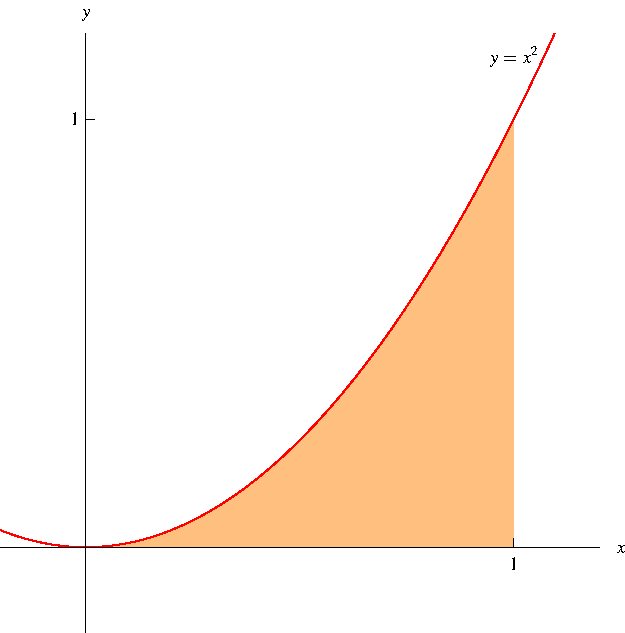
\includegraphics[height=4cm]{integration/pictures/05-01-xsquaredarea.pdf}%
}}%
\only<handout:6| 13>{%
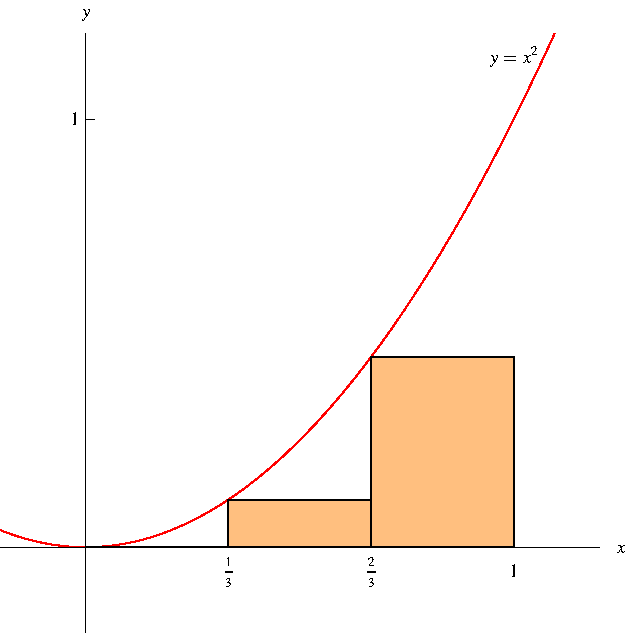
\includegraphics[height=4cm]{integration/pictures/05-01-lefta.pdf}%
}%
\only<handout:0| 14>{%
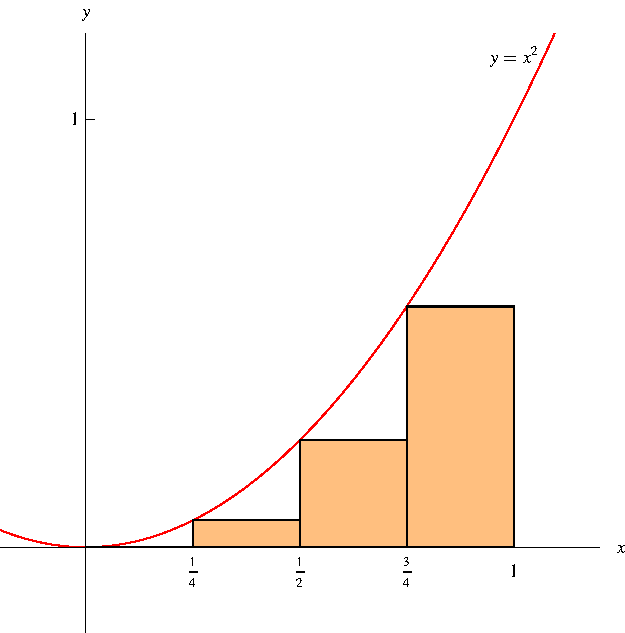
\includegraphics[height=4cm]{integration/pictures/05-01-leftb.pdf}%
}%
\only<handout:0| 15>{%
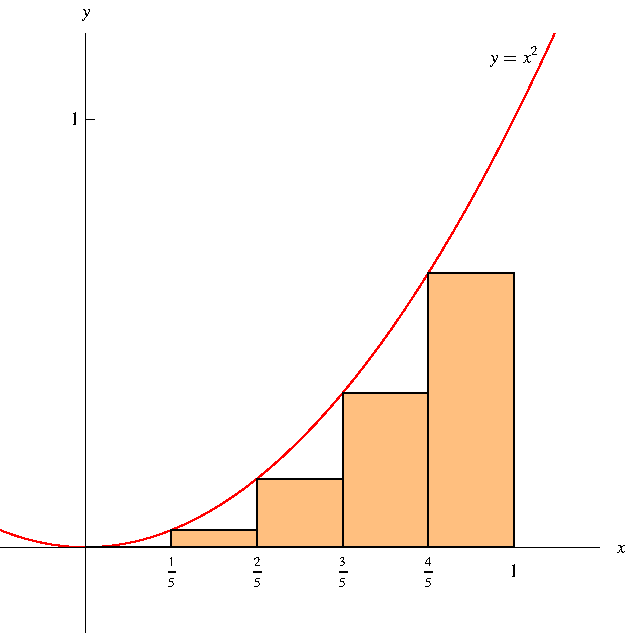
\includegraphics[height=4cm]{integration/pictures/05-01-leftc.pdf}%
}%
\only<handout:0| 16>{%
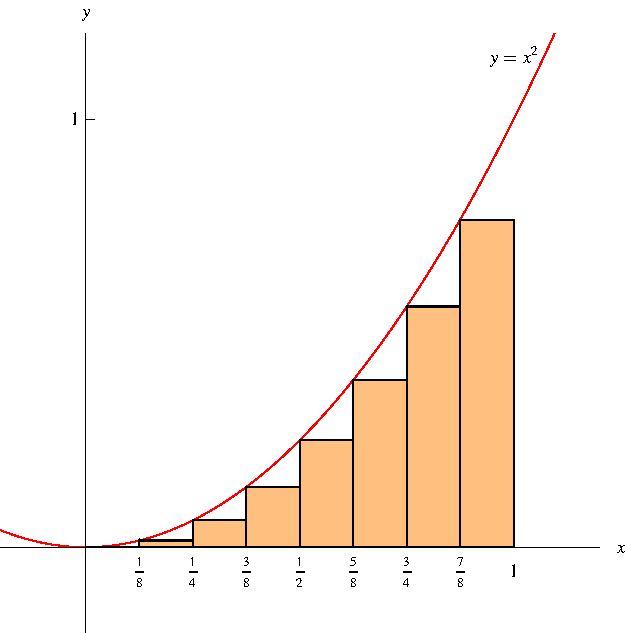
\includegraphics[height=4cm]{integration/pictures/05-01-leftd.pdf}%
}%
\only<handout:0| 17>{%
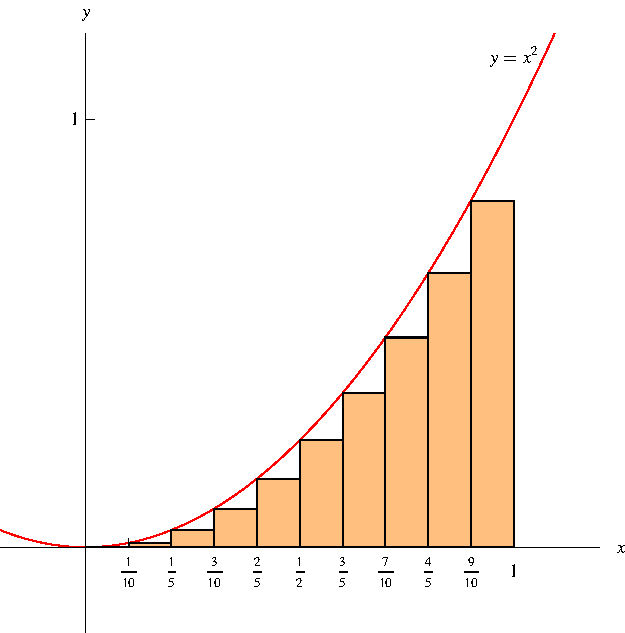
\includegraphics[height=4cm]{integration/pictures/05-01-lefte.pdf}%
}%
\only<handout:0| 18>{%
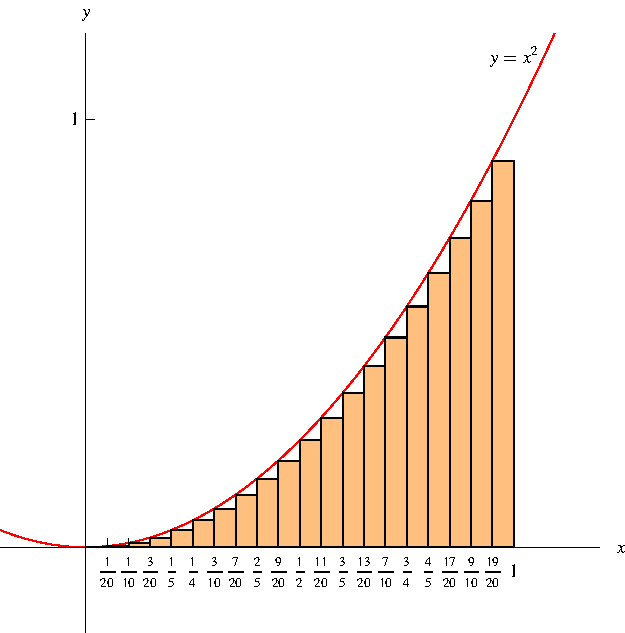
\includegraphics[height=4cm]{integration/pictures/05-01-leftf.pdf}%
}%
\only<handout:0| 19>{%
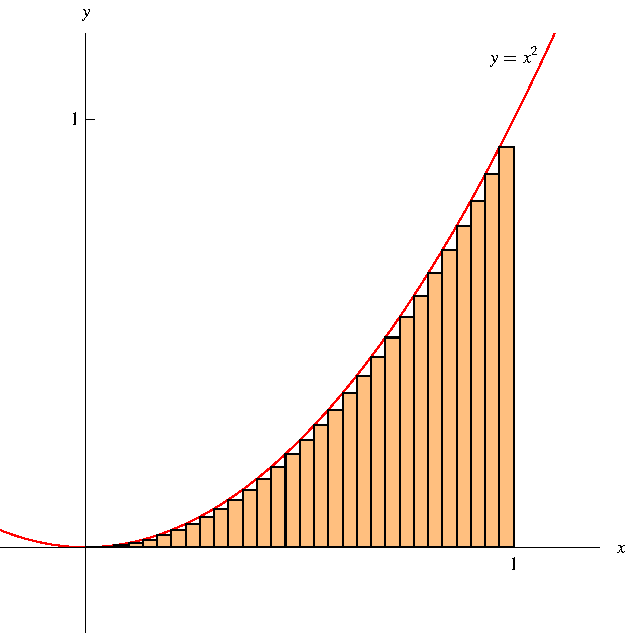
\includegraphics[height=4cm]{integration/pictures/05-01-leftg.pdf}%
}%
\only<handout:7| 20->{%
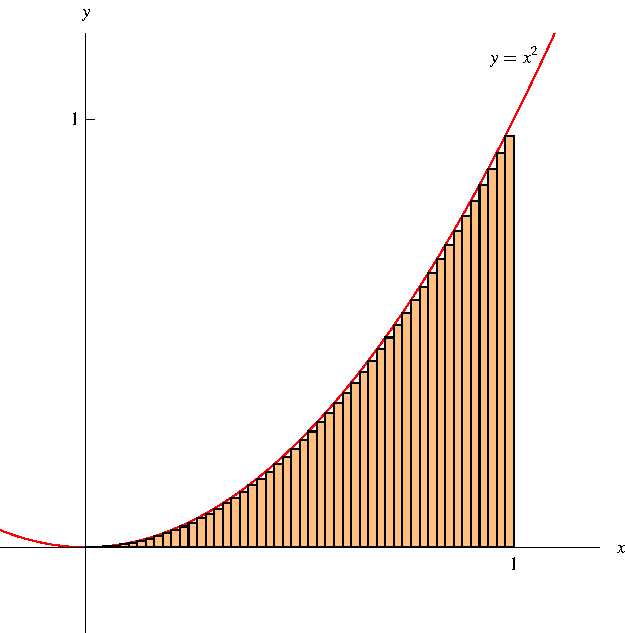
\includegraphics[height=4cm]{integration/pictures/05-01-lefth.pdf}%
}%
\ \only<handout:1| -2>{%
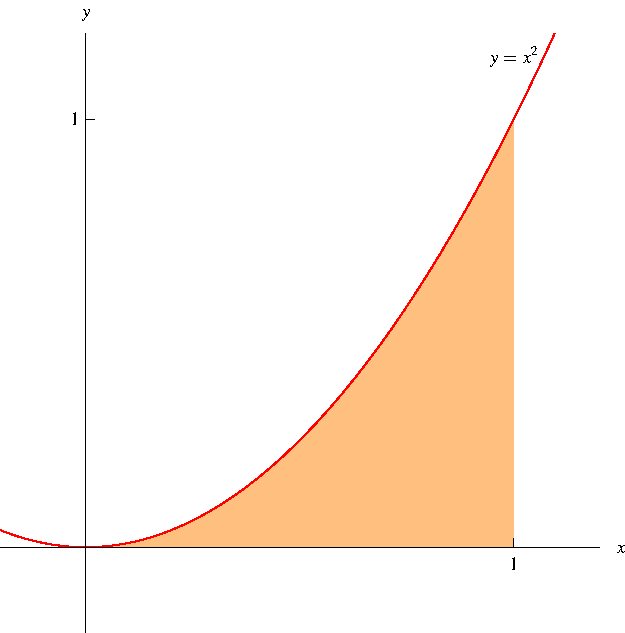
\includegraphics[height=4cm]{integration/pictures/05-01-xsquaredarea.pdf}%
}%
\only<handout:2| 3>{%
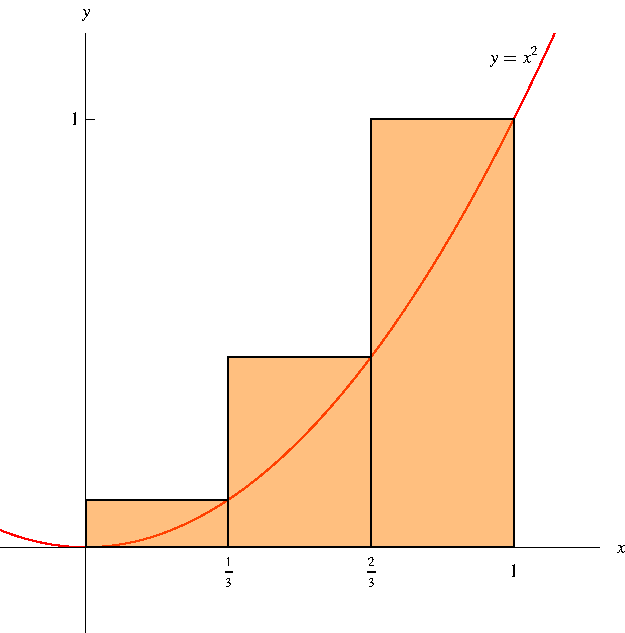
\includegraphics[height=4cm]{integration/pictures/05-01-righta.pdf}%
}%
\only<handout:3| 4>{%
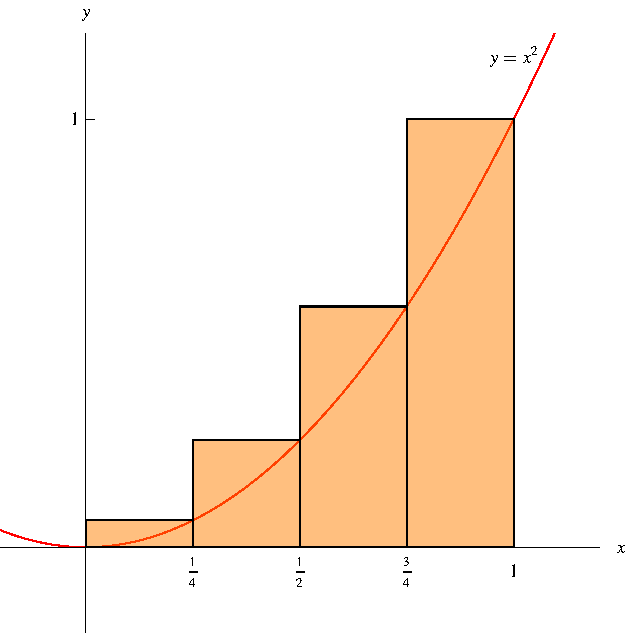
\includegraphics[height=4cm]{integration/pictures/05-01-rightb.pdf}%
}%
\only<handout:0| 5>{%
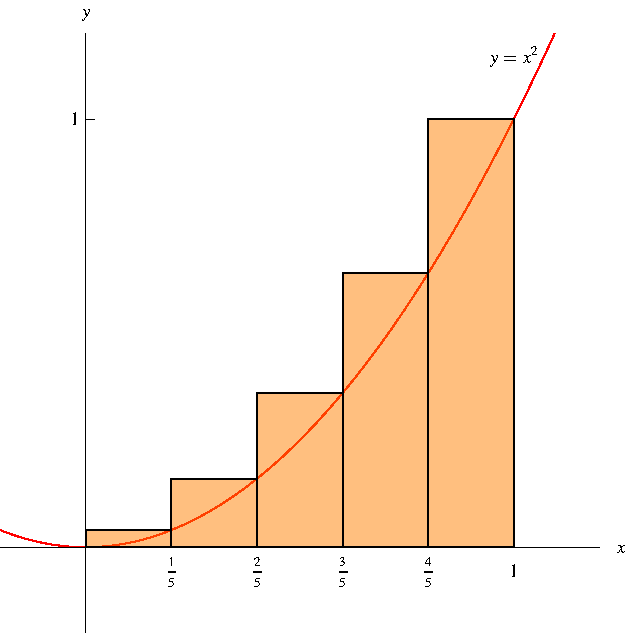
\includegraphics[height=4cm]{integration/pictures/05-01-rightc.pdf}%
}%
\only<handout:4| 6>{%
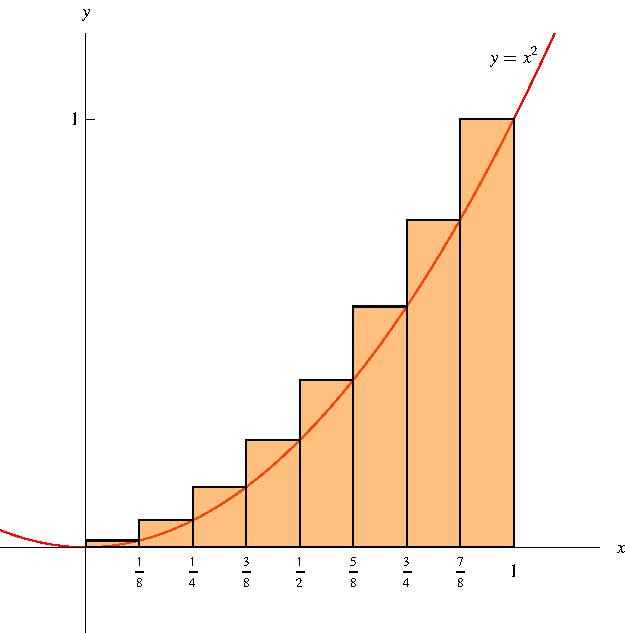
\includegraphics[height=4cm]{integration/pictures/05-01-rightd.pdf}%
}%
\only<handout:0| 7>{%
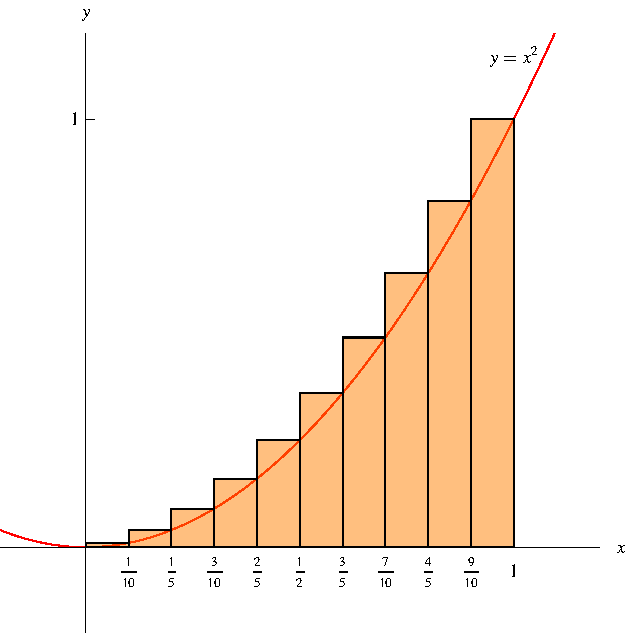
\includegraphics[height=4cm]{integration/pictures/05-01-righte.pdf}%
}%
\only<handout:0| 8>{%
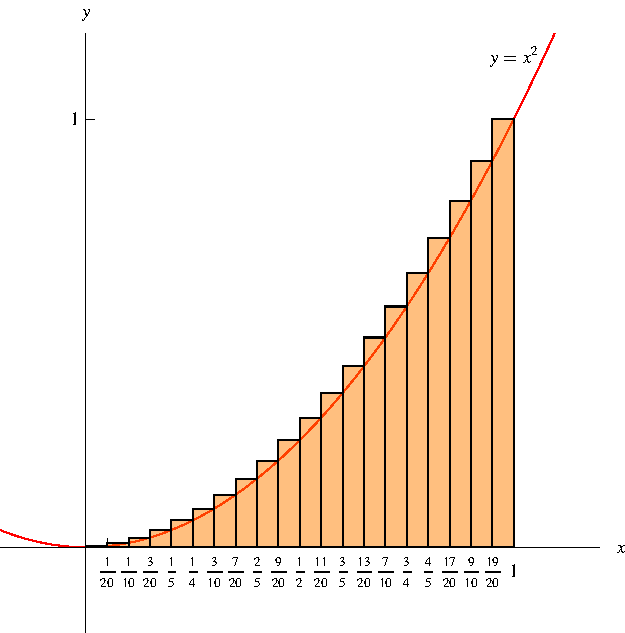
\includegraphics[height=4cm]{integration/pictures/05-01-rightf.pdf}%
}%
\only<handout:0| 9>{%
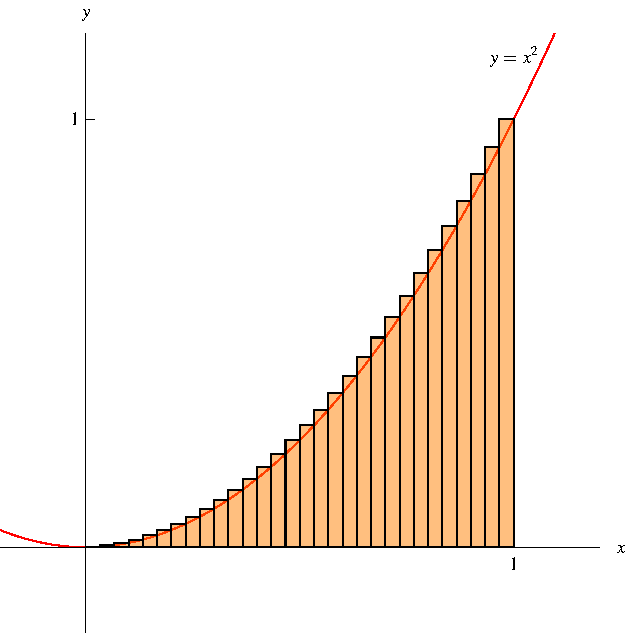
\includegraphics[height=4cm]{integration/pictures/05-01-rightg.pdf}%
}%
\only<handout:5-| 10->{%
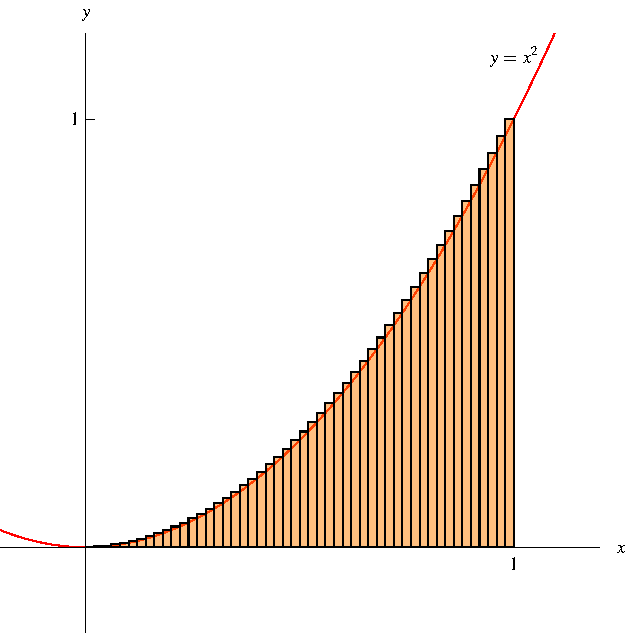
\includegraphics[height=4cm]{integration/pictures/05-01-righth.pdf}%
}%
\end{frame}
% end module areas-intro

% begin module areas-ex1
\begin{frame}
\begin{example}
Find the sum of the areas of the four approximating rectangles obtained using right endpoints.
\begin{columns}[c]
\column{.5\textwidth}
\begin{itemize}
\item<2->  Let $R_4$ denote the sum of the areas of the rectangles.
\item<3-| alert@3-4>  Each rectangle has width $\fcAnswer{4}{\frac{1}{4}}$.
\item<5-| alert@5-6>  The heights are $\fcAnswer{6}{\left( \frac{1}{4}\right)^2}, \fcAnswer{6}{\left( \frac{1}{2}\right)^2}, \fcAnswer{6}{\left(\frac{3}{4}\right)^2}$, and $\fcAnswer{6}{1^2}$.
\item<handout:2-| 9->  A similar calculation works for $L_4$, the sum of the areas of the left endpoint rectangles.
\end{itemize}
\column{.5\textwidth}
\psset{xunit=3cm, yunit=3cm}
\begin{pspicture}(-0.3, -0.3)(1.2,1.2)
\psframe*[linecolor=white](-0.3, -0.3)(1.2,1.2)
\psaxes[ticks=none, labels=none]{<->}(0,0)(-0.3,-0.3)(1.2,1.2)
\tiny
\only<handout:1|-8>{
\psline*[linecolor=\fcColorAreaUnderGraph, linewidth=0.1pt](0.25, 0)(0.25, 0.0625)(0, 0.0625)(0, 0)(0.5, 0)(0.5, 0.25)(0.25, 0.25)(0.25, 0)(0.75, 0)(0.75, 0.5625)(0.5, 0.5625)(0.5, 0)(1, 0)(1, 1)(0.75, 1)(0.75, 0)
\psline[linecolor=blue, linewidth=0.1pt](0.25, 0)(0.25, 0.0625)(0, 0.0625)(0, 0)(0.5, 0)(0.5, 0.25)(0.25, 0.25)(0.25, 0)(0.75, 0)(0.75, 0.5625)(0.5, 0.5625)(0.5, 0)(1, 0)(1, 1)(0.75, 1)(0.75, 0)
}
\only<handout:0|10>{
\psline*[linecolor=gray!35, linewidth=0.1pt](0.25, 0)(0.25, 0.0625)(0, 0.0625)(0, 0)(0.5, 0)(0.5, 0.25)(0.25, 0.25)(0.25, 0)(0.75, 0)(0.75, 0.5625)(0.5, 0.5625)(0.5, 0)
%\psline*[linecolor=gray!10](1, 0)(1, 1)(0.75, 1)(0.75, 0)
\psline[linecolor=blue, linewidth=0.1pt](0.25, 0)(0.25, 0.0625)(0, 0.0625)(0, 0)(0.5, 0)(0.5, 0.25)(0.25, 0.25)(0.25, 0)(0.75, 0)(0.75, 0.5625)(0.5, 0.5625)(0.5, 0)(1, 0)(1, 1)(0.75, 1)(0.75, 0)
}
\only<handout:2|9->{
\psline*[linecolor=\fcColorAreaUnderGraph, linewidth=0.1pt](0, 0)(0, 0)(0.25, 0)(0.25, 0)(0.25, 0)(0.25, 0.0625)(0.5, 0.0625)(0.5, 0)(0.5, 0)(0.5, 0.25)(0.75, 0.25)(0.75, 0)(0.75, 0)(0.75, 0.5625)(1, 0.5625)(1, 0)
\psline[linecolor=blue, linewidth=0.1pt](0, 0)(0, 0)(0.25, 0)(0.25, 0)(0.25, 0)(0.25, 0.0625)(0.5, 0.0625)(0.5, 0)(0.5, 0)(0.5, 0.25)(0.75, 0.25)(0.75, 0)(0.75, 0)(0.75, 0.5625)(1, 0.5625)(1, 0)
}
\rput[t](0.25,-0.03){$\frac{1}{4}$}\rput[t](0.5,-0.03){$\frac{1}{2}$}\rput[t](0.75,-0.03){$\frac{3}{4}$}\rput[t](1,-0.03){$1$}
%Function formula: (x)^{2}
\rput[t](0.5,1){$y=x^{2}$}
\psplot[linecolor=red, plotpoints=1000]{0}{1}{x 2 exp }
\end{pspicture}
%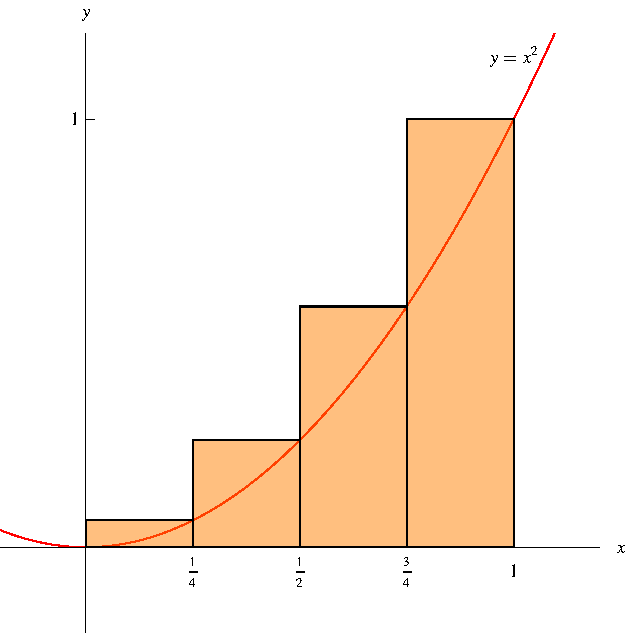
\includegraphics[height=4.5cm]{integration/pictures/05-01-rightb.pdf}%
\end{columns}
\uncover<7->{%
\abovedisplayskip=0pt
\belowdisplayskip=0pt
\[
R_4 = \alertNoH{10}{\frac{1}{4}\cdot \left(\frac{1}{4}\right)^2}%
+ \alertNoH{10}{\frac{1}{4}\cdot \left(\frac{1}{2}\right)^2}%
+ \alertNoH{10}{\frac{1}{4}\cdot \left(\frac{3}{4}\right)^2}%
+ \frac{1}{4}\cdot \left( 1\right)^2%
\uncover<8->{ = \frac{15}{32} = 0.46875}%
\]
}%
\uncover<handout:2-| 9,10,11->{%
\abovedisplayskip=0pt
\belowdisplayskip=0pt
\[
L_4 = \frac{1}{4}\cdot \left( 0\right)^2%
+\alertNoH{10}{ \frac{1}{4}\cdot \left(\frac{1}{4}\right)^2}%
+ \alertNoH{10}{\frac{1}{4}\cdot \left(\frac{1}{2}\right)^2}%
+\alertNoH{10}{ \frac{1}{4}\cdot \left( \frac{3}{4}\right)^2}%
\uncover<11->{ = \frac{7}{32} = 0.21875}%
\]
}%
\vspace{-.1in}
\end{example}
\end{frame}
% end module areas-ex1

% begin module areas-ex2
\begin{frame}
\begin{example}
For the region $S$ underneath the parabola $y = x^2$ from $0$ to $1$, show that the area under the approximating rectangles approaches $\frac{1}{3}$, that is,
\begin{columns}[c]
\column{.6\textwidth}
\abovedisplayskip=0pt
\belowdisplayskip=0pt
\[
\lim_{n\to\infty}R_n = \frac{1}{3}.
\]
\begin{itemize}
\item<9-| alert@9-10>  Each rectangle has width $\fcAnswer{10}{\frac{1}{n}}$.
\item<9-| alert@11-12>  The heights are $ \fcAnswerUncover{9}{12}{\left( \frac{1}{n}\right)^2}, \fcAnswerUncover{9}{12}{\left( \frac{2}{n}\right)^2},$ $\ldots ,$ $\fcAnswerUncover{9}{12}{\left( \frac{n}{n}\right)^2}$.
\item<15->  New formula:
\item<15-| alert@15-17>  $1^2 + 2^2 + 3^2 + \cdots + n^2 $ $ =\fcAnswer{16}{ \frac{n(n+1)(2n+1)}{6}}$.
\end{itemize}
\column{.4\textwidth}
\psset{xunit=2cm, yunit=2cm}
\begin{pspicture}(-5, -5)(5,5)
\psline{linecolor=red!1}(0, -0.3)(0, -0.31)
\psframe*[linecolor=white](-5,-5)(5,5)
\tiny
%Function formula: x^{2}
\rput(0.9,1.3){$y=x^{2}$}
\uncover<handout:0|2>{
%approximation 1/3
\psline*[linecolor=\fcColorAreaUnderGraph, linewidth=0.1pt](0.333333, 0)(0.333333, 0.111111)(0, 0.111111)(0, 0)(0.666667, 0)(0.666667, 0.444444)(0.333333, 0.444444)(0.333333, 0)(1, 0)(1, 1)(0.666667, 1)(0.666667, 0)
\psline[linecolor=blue, linewidth=0.1pt](0.333333, 0)(0.333333, 0.111111)(0, 0.111111)(0, 0)(0.666667, 0)(0.666667, 0.444444)(0.333333, 0.444444)(0.333333, 0)(1, 0)(1, 1)(0.666667, 1)(0.666667, 0)
\rput[t](0.333333,-0.03){$\frac{1}{3}$}\rput[t](0.666667,-0.03){$\frac{2}{3}$}\rput[t](1,-0.03){$1$}
}
\uncover<handout:0|3>{
%approximation 1/4
\psline*[linecolor=\fcColorAreaUnderGraph, linewidth=0.1pt](0.25, 0)(0.25, 0.0625)(0, 0.0625)(0, 0)(0.5, 0)(0.5, 0.25)(0.25, 0.25)(0.25, 0)(0.75, 0)(0.75, 0.5625)(0.5, 0.5625)(0.5, 0)(1, 0)(1, 1)(0.75, 1)(0.75, 0)
\psline[linecolor=blue, linewidth=0.1pt](0.25, 0)(0.25, 0.0625)(0, 0.0625)(0, 0)(0.5, 0)(0.5, 0.25)(0.25, 0.25)(0.25, 0)(0.75, 0)(0.75, 0.5625)(0.5, 0.5625)(0.5, 0)(1, 0)(1, 1)(0.75, 1)(0.75, 0)
\rput[t](0.25,-0.03){$\frac{1}{4}$}\rput[t](0.5,-0.03){$\frac{1}{2}$}\rput[t](0.75,-0.03){$\frac{3}{4}$}\rput[t](1,-0.03){$1$}
}
\uncover<handout:0|4>{
%approximation 1/5
\psline*[linecolor=\fcColorAreaUnderGraph, linewidth=0.1pt](0.2, 0)(0.2, 0.04)(0, 0.04)(0, 0)(0.4, 0)(0.4, 0.16)(0.2, 0.16)(0.2, 0)(0.6, 0)(0.6, 0.36)(0.4, 0.36)(0.4, 0)(0.8, 0)(0.8, 0.64)(0.6, 0.64)(0.6, 0)(1, 0)(1, 1)(0.8, 1)(0.8, 0)
\psline[linecolor=blue, linewidth=0.1pt](0.2, 0)(0.2, 0.04)(0, 0.04)(0, 0)(0.4, 0)(0.4, 0.16)(0.2, 0.16)(0.2, 0)(0.6, 0)(0.6, 0.36)(0.4, 0.36)(0.4, 0)(0.8, 0)(0.8, 0.64)(0.6, 0.64)(0.6, 0)(1, 0)(1, 1)(0.8, 1)(0.8, 0)
\rput[t](0.2,-0.03){$\frac{1}{5}$}\rput[t](0.4,-0.03){$\frac{2}{5}$}\rput[t](0.6,-0.03){$\frac{3}{5}$}\rput[t](0.8,-0.03){$\frac{4}{5}$}\rput[t](1,-0.03){$1$}
}
\uncover<handout:0|5>{
%approximation 1/8
\psline*[linecolor=\fcColorAreaUnderGraph, linewidth=0.1pt](0.125, 0)(0.125, 0.015625)(0, 0.015625)(0, 0)(0.25, 0)(0.25, 0.0625)(0.125, 0.0625)(0.125, 0)(0.375, 0)(0.375, 0.140625)(0.25, 0.140625)(0.25, 0)(0.5, 0)(0.5, 0.25)(0.375, 0.25)(0.375, 0)(0.625, 0)(0.625, 0.390625)(0.5, 0.390625)(0.5, 0)(0.75, 0)(0.75, 0.5625)(0.625, 0.5625)(0.625, 0)(0.875, 0)(0.875, 0.765625)(0.75, 0.765625)(0.75, 0)(1, 0)(1, 1)(0.875, 1)(0.875, 0)
\psline[linecolor=blue, linewidth=0.1pt](0.125, 0)(0.125, 0.015625)(0, 0.015625)(0, 0)(0.25, 0)(0.25, 0.0625)(0.125, 0.0625)(0.125, 0)(0.375, 0)(0.375, 0.140625)(0.25, 0.140625)(0.25, 0)(0.5, 0)(0.5, 0.25)(0.375, 0.25)(0.375, 0)(0.625, 0)(0.625, 0.390625)(0.5, 0.390625)(0.5, 0)(0.75, 0)(0.75, 0.5625)(0.625, 0.5625)(0.625, 0)(0.875, 0)(0.875, 0.765625)(0.75, 0.765625)(0.75, 0)(1, 0)(1, 1)(0.875, 1)(0.875, 0)
\rput[t](0.125,-0.03){$\frac{1}{8}$}\rput[t](0.25,-0.03){$\frac{1}{4}$}\rput[t](0.375,-0.03){$\frac{3}{8}$}\rput[t](0.5,-0.03){$\frac{1}{2}$}\rput[t](0.625,-0.03){$\frac{5}{8}$}\rput[t](0.75,-0.03){$\frac{3}{4}$}\rput[t](0.875,-0.03){$\frac{7}{8}$}\rput[t](1,-0.03){$1$}
}
\uncover<handout:1|6>{
%approximation 1/10
\psline*[linecolor=\fcColorAreaUnderGraph, linewidth=0.1pt](0.1, 0)(0.1, 0.01)(0, 0.01)(0, 0)(0.2, 0)(0.2, 0.04)(0.1, 0.04)(0.1, 0)(0.3, 0)(0.3, 0.09)(0.2, 0.09)(0.2, 0)(0.4, 0)(0.4, 0.16)(0.3, 0.16)(0.3, 0)(0.5, 0)(0.5, 0.25)(0.4, 0.25)(0.4, 0)(0.6, 0)(0.6, 0.36)(0.5, 0.36)(0.5, 0)(0.7, 0)(0.7, 0.49)(0.6, 0.49)(0.6, 0)(0.8, 0)(0.8, 0.64)(0.7, 0.64)(0.7, 0)(0.9, 0)(0.9, 0.81)(0.8, 0.81)(0.8, 0)(1, 0)(1, 1)(0.9, 1)(0.9, 0)
\psline[linecolor=blue, linewidth=0.1pt](0.1, 0)(0.1, 0.01)(0, 0.01)(0, 0)(0.2, 0)(0.2, 0.04)(0.1, 0.04)(0.1, 0)(0.3, 0)(0.3, 0.09)(0.2, 0.09)(0.2, 0)(0.4, 0)(0.4, 0.16)(0.3, 0.16)(0.3, 0)(0.5, 0)(0.5, 0.25)(0.4, 0.25)(0.4, 0)(0.6, 0)(0.6, 0.36)(0.5, 0.36)(0.5, 0)(0.7, 0)(0.7, 0.49)(0.6, 0.49)(0.6, 0)(0.8, 0)(0.8, 0.64)(0.7, 0.64)(0.7, 0)(0.9, 0)(0.9, 0.81)(0.8, 0.81)(0.8, 0)(1, 0)(1, 1)(0.9, 1)(0.9, 0)
\rput[t](0.1,-0.03){$\frac{1}{10}$}\rput[t](0.2,-0.03){$\frac{1}{5}$}\rput[t](0.3,-0.03){$\frac{3}{10}$}\rput[t](0.4,-0.03){$\frac{2}{5}$}\rput[t](0.5,-0.03){$\frac{1}{2}$}\rput[t](0.6,-0.03){$\frac{3}{5}$}\rput[t](0.7,-0.03){$\frac{7}{10}$}\rput[t](0.8,-0.03){$\frac{4}{5}$}\rput[t](0.9,-0.03){$\frac{9}{10}$}\rput[t](1,-0.03){$1$}
}
\uncover<handout:0|7>{
%approximation 1/20
\psline*[linecolor=\fcColorAreaUnderGraph, linewidth=0.1pt](0.05, 0)(0.05, 0.0025)(0, 0.0025)(0, 0)(0.1, 0)(0.1, 0.01)(0.05, 0.01)(0.05, 0)(0.15, 0)(0.15, 0.0225)(0.1, 0.0225)(0.1, 0)(0.2, 0)(0.2, 0.04)(0.15, 0.04)(0.15, 0)(0.25, 0)(0.25, 0.0625)(0.2, 0.0625)(0.2, 0)(0.3, 0)(0.3, 0.09)(0.25, 0.09)(0.25, 0)(0.35, 0)(0.35, 0.1225)(0.3, 0.1225)(0.3, 0)(0.4, 0)(0.4, 0.16)(0.35, 0.16)(0.35, 0)(0.45, 0)(0.45, 0.2025)(0.4, 0.2025)(0.4, 0)(0.5, 0)(0.5, 0.25)(0.45, 0.25)(0.45, 0)(0.55, 0)(0.55, 0.3025)(0.5, 0.3025)(0.5, 0)(0.6, 0)(0.6, 0.36)(0.55, 0.36)(0.55, 0)(0.65, 0)(0.65, 0.4225)(0.6, 0.4225)(0.6, 0)(0.7, 0)(0.7, 0.49)(0.65, 0.49)(0.65, 0)(0.75, 0)(0.75, 0.5625)(0.7, 0.5625)(0.7, 0)(0.8, 0)(0.8, 0.64)(0.75, 0.64)(0.75, 0)(0.85, 0)(0.85, 0.7225)(0.8, 0.7225)(0.8, 0)(0.9, 0)(0.9, 0.81)(0.85, 0.81)(0.85, 0)(0.95, 0)(0.95, 0.9025)(0.9, 0.9025)(0.9, 0)(1, 0)(1, 1)(0.95, 1)(0.95, 0)
\psline[linecolor=blue, linewidth=0.1pt](0.05, 0)(0.05, 0.0025)(0, 0.0025)(0, 0)(0.1, 0)(0.1, 0.01)(0.05, 0.01)(0.05, 0)(0.15, 0)(0.15, 0.0225)(0.1, 0.0225)(0.1, 0)(0.2, 0)(0.2, 0.04)(0.15, 0.04)(0.15, 0)(0.25, 0)(0.25, 0.0625)(0.2, 0.0625)(0.2, 0)(0.3, 0)(0.3, 0.09)(0.25, 0.09)(0.25, 0)(0.35, 0)(0.35, 0.1225)(0.3, 0.1225)(0.3, 0)(0.4, 0)(0.4, 0.16)(0.35, 0.16)(0.35, 0)(0.45, 0)(0.45, 0.2025)(0.4, 0.2025)(0.4, 0)(0.5, 0)(0.5, 0.25)(0.45, 0.25)(0.45, 0)(0.55, 0)(0.55, 0.3025)(0.5, 0.3025)(0.5, 0)(0.6, 0)(0.6, 0.36)(0.55, 0.36)(0.55, 0)(0.65, 0)(0.65, 0.4225)(0.6, 0.4225)(0.6, 0)(0.7, 0)(0.7, 0.49)(0.65, 0.49)(0.65, 0)(0.75, 0)(0.75, 0.5625)(0.7, 0.5625)(0.7, 0)(0.8, 0)(0.8, 0.64)(0.75, 0.64)(0.75, 0)(0.85, 0)(0.85, 0.7225)(0.8, 0.7225)(0.8, 0)(0.9, 0)(0.9, 0.81)(0.85, 0.81)(0.85, 0)(0.95, 0)(0.95, 0.9025)(0.9, 0.9025)(0.9, 0)(1, 0)(1, 1)(0.95, 1)(0.95, 0)
}
\uncover<handout:0|8>{
%approximation 1/30
\psline*[linecolor=\fcColorAreaUnderGraph, linewidth=0.1pt](0.0333333, 0)(0.0333333, 0.00111111)(0, 0.00111111)(0, 0)(0.0666667, 0)(0.0666667, 0.00444444)(0.0333333, 0.00444444)(0.0333333, 0)(0.1, 0)(0.1, 0.01)(0.0666667, 0.01)(0.0666667, 0)(0.133333, 0)(0.133333, 0.0177778)(0.1, 0.0177778)(0.1, 0)(0.166667, 0)(0.166667, 0.0277778)(0.133333, 0.0277778)(0.133333, 0)(0.2, 0)(0.2, 0.04)(0.166667, 0.04)(0.166667, 0)(0.233333, 0)(0.233333, 0.0544444)(0.2, 0.0544444)(0.2, 0)(0.266667, 0)(0.266667, 0.0711111)(0.233333, 0.0711111)(0.233333, 0)(0.3, 0)(0.3, 0.09)(0.266667, 0.09)(0.266667, 0)(0.333333, 0)(0.333333, 0.111111)(0.3, 0.111111)(0.3, 0)(0.366667, 0)(0.366667, 0.134444)(0.333333, 0.134444)(0.333333, 0)(0.4, 0)(0.4, 0.16)(0.366667, 0.16)(0.366667, 0)(0.433333, 0)(0.433333, 0.187778)(0.4, 0.187778)(0.4, 0)(0.466667, 0)(0.466667, 0.217778)(0.433333, 0.217778)(0.433333, 0)(0.5, 0)(0.5, 0.25)(0.466667, 0.25)(0.466667, 0)(0.533333, 0)(0.533333, 0.284444)(0.5, 0.284444)(0.5, 0)(0.566667, 0)(0.566667, 0.321111)(0.533333, 0.321111)(0.533333, 0)(0.6, 0)(0.6, 0.36)(0.566667, 0.36)(0.566667, 0)(0.633333, 0)(0.633333, 0.401111)(0.6, 0.401111)(0.6, 0)(0.666667, 0)(0.666667, 0.444444)(0.633333, 0.444444)(0.633333, 0)(0.7, 0)(0.7, 0.49)(0.666667, 0.49)(0.666667, 0)(0.733333, 0)(0.733333, 0.537778)(0.7, 0.537778)(0.7, 0)(0.766667, 0)(0.766667, 0.587778)(0.733333, 0.587778)(0.733333, 0)(0.8, 0)(0.8, 0.64)(0.766667, 0.64)(0.766667, 0)(0.833333, 0)(0.833333, 0.694444)(0.8, 0.694444)(0.8, 0)(0.866667, 0)(0.866667, 0.751111)(0.833333, 0.751111)(0.833333, 0)(0.9, 0)(0.9, 0.81)(0.866667, 0.81)(0.866667, 0)(0.933333, 0)(0.933333, 0.871111)(0.9, 0.871111)(0.9, 0)(0.966667, 0)(0.966667, 0.934444)(0.933333, 0.934444)(0.933333, 0)(1, 0)(1, 1)(0.966667, 1)(0.966667, 0)
\psline[linecolor=blue, linewidth=0.1pt](0.0333333, 0)(0.0333333, 0.00111111)(0, 0.00111111)(0, 0)(0.0666667, 0)(0.0666667, 0.00444444)(0.0333333, 0.00444444)(0.0333333, 0)(0.1, 0)(0.1, 0.01)(0.0666667, 0.01)(0.0666667, 0)(0.133333, 0)(0.133333, 0.0177778)(0.1, 0.0177778)(0.1, 0)(0.166667, 0)(0.166667, 0.0277778)(0.133333, 0.0277778)(0.133333, 0)(0.2, 0)(0.2, 0.04)(0.166667, 0.04)(0.166667, 0)(0.233333, 0)(0.233333, 0.0544444)(0.2, 0.0544444)(0.2, 0)(0.266667, 0)(0.266667, 0.0711111)(0.233333, 0.0711111)(0.233333, 0)(0.3, 0)(0.3, 0.09)(0.266667, 0.09)(0.266667, 0)(0.333333, 0)(0.333333, 0.111111)(0.3, 0.111111)(0.3, 0)(0.366667, 0)(0.366667, 0.134444)(0.333333, 0.134444)(0.333333, 0)(0.4, 0)(0.4, 0.16)(0.366667, 0.16)(0.366667, 0)(0.433333, 0)(0.433333, 0.187778)(0.4, 0.187778)(0.4, 0)(0.466667, 0)(0.466667, 0.217778)(0.433333, 0.217778)(0.433333, 0)(0.5, 0)(0.5, 0.25)(0.466667, 0.25)(0.466667, 0)(0.533333, 0)(0.533333, 0.284444)(0.5, 0.284444)(0.5, 0)(0.566667, 0)(0.566667, 0.321111)(0.533333, 0.321111)(0.533333, 0)(0.6, 0)(0.6, 0.36)(0.566667, 0.36)(0.566667, 0)(0.633333, 0)(0.633333, 0.401111)(0.6, 0.401111)(0.6, 0)(0.666667, 0)(0.666667, 0.444444)(0.633333, 0.444444)(0.633333, 0)(0.7, 0)(0.7, 0.49)(0.666667, 0.49)(0.666667, 0)(0.733333, 0)(0.733333, 0.537778)(0.7, 0.537778)(0.7, 0)(0.766667, 0)(0.766667, 0.587778)(0.733333, 0.587778)(0.733333, 0)(0.8, 0)(0.8, 0.64)(0.766667, 0.64)(0.766667, 0)(0.833333, 0)(0.833333, 0.694444)(0.8, 0.694444)(0.8, 0)(0.866667, 0)(0.866667, 0.751111)(0.833333, 0.751111)(0.833333, 0)(0.9, 0)(0.9, 0.81)(0.866667, 0.81)(0.866667, 0)(0.933333, 0)(0.933333, 0.871111)(0.9, 0.871111)(0.9, 0)(0.966667, 0)(0.966667, 0.934444)(0.933333, 0.934444)(0.933333, 0)(1, 0)(1, 1)(0.966667, 1)(0.966667, 0)
}
\uncover<handout:0|9->{
%approximation 1/40
\psline*[linecolor=\fcColorAreaUnderGraph, linewidth=0.1pt](0.025, 0)(0.025, 0.000625)(0, 0.000625)(0, 0)(0.05, 0)(0.05, 0.0025)(0.025, 0.0025)(0.025, 0)(0.075, 0)(0.075, 0.005625)(0.05, 0.005625)(0.05, 0)(0.1, 0)(0.1, 0.01)(0.075, 0.01)(0.075, 0)(0.125, 0)(0.125, 0.015625)(0.1, 0.015625)(0.1, 0)(0.15, 0)(0.15, 0.0225)(0.125, 0.0225)(0.125, 0)(0.175, 0)(0.175, 0.030625)(0.15, 0.030625)(0.15, 0)(0.2, 0)(0.2, 0.04)(0.175, 0.04)(0.175, 0)(0.225, 0)(0.225, 0.050625)(0.2, 0.050625)(0.2, 0)(0.25, 0)(0.25, 0.0625)(0.225, 0.0625)(0.225, 0)(0.275, 0)(0.275, 0.075625)(0.25, 0.075625)(0.25, 0)(0.3, 0)(0.3, 0.09)(0.275, 0.09)(0.275, 0)(0.325, 0)(0.325, 0.105625)(0.3, 0.105625)(0.3, 0)(0.35, 0)(0.35, 0.1225)(0.325, 0.1225)(0.325, 0)(0.375, 0)(0.375, 0.140625)(0.35, 0.140625)(0.35, 0)(0.4, 0)(0.4, 0.16)(0.375, 0.16)(0.375, 0)(0.425, 0)(0.425, 0.180625)(0.4, 0.180625)(0.4, 0)(0.45, 0)(0.45, 0.2025)(0.425, 0.2025)(0.425, 0)(0.475, 0)(0.475, 0.225625)(0.45, 0.225625)(0.45, 0)(0.5, 0)(0.5, 0.25)(0.475, 0.25)(0.475, 0)(0.525, 0)(0.525, 0.275625)(0.5, 0.275625)(0.5, 0)(0.55, 0)(0.55, 0.3025)(0.525, 0.3025)(0.525, 0)(0.575, 0)(0.575, 0.330625)(0.55, 0.330625)(0.55, 0)(0.6, 0)(0.6, 0.36)(0.575, 0.36)(0.575, 0)(0.625, 0)(0.625, 0.390625)(0.6, 0.390625)(0.6, 0)(0.65, 0)(0.65, 0.4225)(0.625, 0.4225)(0.625, 0)(0.675, 0)(0.675, 0.455625)(0.65, 0.455625)(0.65, 0)(0.7, 0)(0.7, 0.49)(0.675, 0.49)(0.675, 0)(0.725, 0)(0.725, 0.525625)(0.7, 0.525625)(0.7, 0)(0.75, 0)(0.75, 0.5625)(0.725, 0.5625)(0.725, 0)(0.775, 0)(0.775, 0.600625)(0.75, 0.600625)(0.75, 0)(0.8, 0)(0.8, 0.64)(0.775, 0.64)(0.775, 0)(0.825, 0)(0.825, 0.680625)(0.8, 0.680625)(0.8, 0)(0.85, 0)(0.85, 0.7225)(0.825, 0.7225)(0.825, 0)(0.875, 0)(0.875, 0.765625)(0.85, 0.765625)(0.85, 0)(0.9, 0)(0.9, 0.81)(0.875, 0.81)(0.875, 0)(0.925, 0)(0.925, 0.855625)(0.9, 0.855625)(0.9, 0)(0.95, 0)(0.95, 0.9025)(0.925, 0.9025)(0.925, 0)(0.975, 0)(0.975, 0.950625)(0.95, 0.950625)(0.95, 0)(1, 0)(1, 1)(0.975, 1)(0.975, 0)
\psline[linecolor=blue, linewidth=0.1pt](0.025, 0)(0.025, 0.000625)(0, 0.000625)(0, 0)(0.05, 0)(0.05, 0.0025)(0.025, 0.0025)(0.025, 0)(0.075, 0)(0.075, 0.005625)(0.05, 0.005625)(0.05, 0)(0.1, 0)(0.1, 0.01)(0.075, 0.01)(0.075, 0)(0.125, 0)(0.125, 0.015625)(0.1, 0.015625)(0.1, 0)(0.15, 0)(0.15, 0.0225)(0.125, 0.0225)(0.125, 0)(0.175, 0)(0.175, 0.030625)(0.15, 0.030625)(0.15, 0)(0.2, 0)(0.2, 0.04)(0.175, 0.04)(0.175, 0)(0.225, 0)(0.225, 0.050625)(0.2, 0.050625)(0.2, 0)(0.25, 0)(0.25, 0.0625)(0.225, 0.0625)(0.225, 0)(0.275, 0)(0.275, 0.075625)(0.25, 0.075625)(0.25, 0)(0.3, 0)(0.3, 0.09)(0.275, 0.09)(0.275, 0)(0.325, 0)(0.325, 0.105625)(0.3, 0.105625)(0.3, 0)(0.35, 0)(0.35, 0.1225)(0.325, 0.1225)(0.325, 0)(0.375, 0)(0.375, 0.140625)(0.35, 0.140625)(0.35, 0)(0.4, 0)(0.4, 0.16)(0.375, 0.16)(0.375, 0)(0.425, 0)(0.425, 0.180625)(0.4, 0.180625)(0.4, 0)(0.45, 0)(0.45, 0.2025)(0.425, 0.2025)(0.425, 0)(0.475, 0)(0.475, 0.225625)(0.45, 0.225625)(0.45, 0)(0.5, 0)(0.5, 0.25)(0.475, 0.25)(0.475, 0)(0.525, 0)(0.525, 0.275625)(0.5, 0.275625)(0.5, 0)(0.55, 0)(0.55, 0.3025)(0.525, 0.3025)(0.525, 0)(0.575, 0)(0.575, 0.330625)(0.55, 0.330625)(0.55, 0)(0.6, 0)(0.6, 0.36)(0.575, 0.36)(0.575, 0)(0.625, 0)(0.625, 0.390625)(0.6, 0.390625)(0.6, 0)(0.65, 0)(0.65, 0.4225)(0.625, 0.4225)(0.625, 0)(0.675, 0)(0.675, 0.455625)(0.65, 0.455625)(0.65, 0)(0.7, 0)(0.7, 0.49)(0.675, 0.49)(0.675, 0)(0.725, 0)(0.725, 0.525625)(0.7, 0.525625)(0.7, 0)(0.75, 0)(0.75, 0.5625)(0.725, 0.5625)(0.725, 0)(0.775, 0)(0.775, 0.600625)(0.75, 0.600625)(0.75, 0)(0.8, 0)(0.8, 0.64)(0.775, 0.64)(0.775, 0)(0.825, 0)(0.825, 0.680625)(0.8, 0.680625)(0.8, 0)(0.85, 0)(0.85, 0.7225)(0.825, 0.7225)(0.825, 0)(0.875, 0)(0.875, 0.765625)(0.85, 0.765625)(0.85, 0)(0.9, 0)(0.9, 0.81)(0.875, 0.81)(0.875, 0)(0.925, 0)(0.925, 0.855625)(0.9, 0.855625)(0.9, 0)(0.95, 0)(0.95, 0.9025)(0.925, 0.9025)(0.925, 0)(0.975, 0)(0.975, 0.950625)(0.95, 0.950625)(0.95, 0)(1, 0)(1, 1)(0.975, 1)(0.975, 0)
}
\psaxes[ticks=none, labels=none]{<->}(0,0)(-0.1,-0.1)(1.4,1.4)
\psplot[linecolor=red, plotpoints=1000]{0}{1.15}{x 2 exp }
\end{pspicture}
%\only<handout:0| -1>{%
%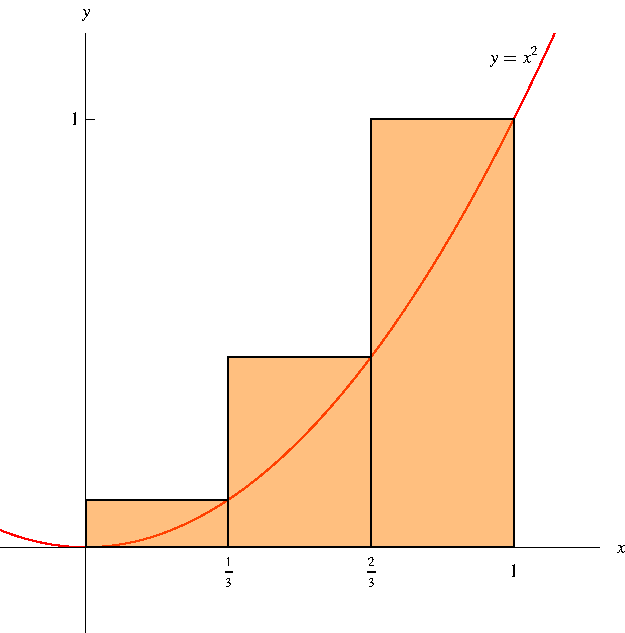
\includegraphics[height=4.5cm]{integration/pictures/05-01-righta.pdf}%
%}%
%\only<handout:0| 2>{%
%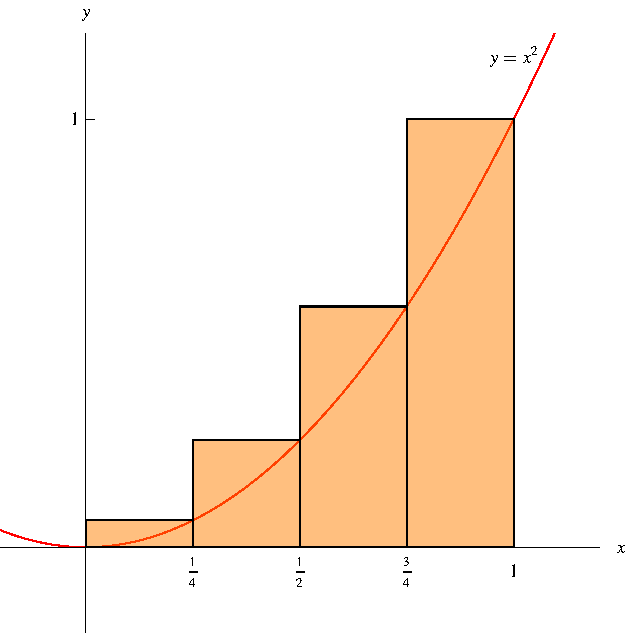
\includegraphics[height=4.5cm]{integration/pictures/05-01-rightb.pdf}%
%}%
%\only<handout:0| 3>{%
%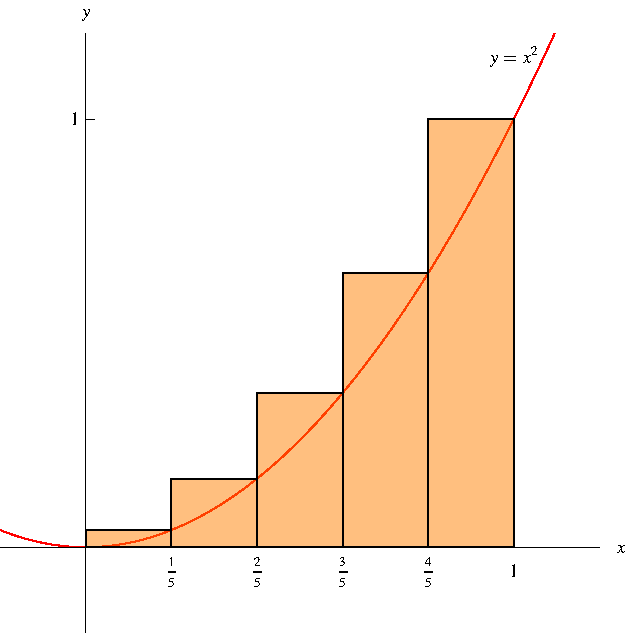
\includegraphics[height=4.5cm]{integration/pictures/05-01-rightc.pdf}%
%}%
%\only<handout:0| 4>{%
%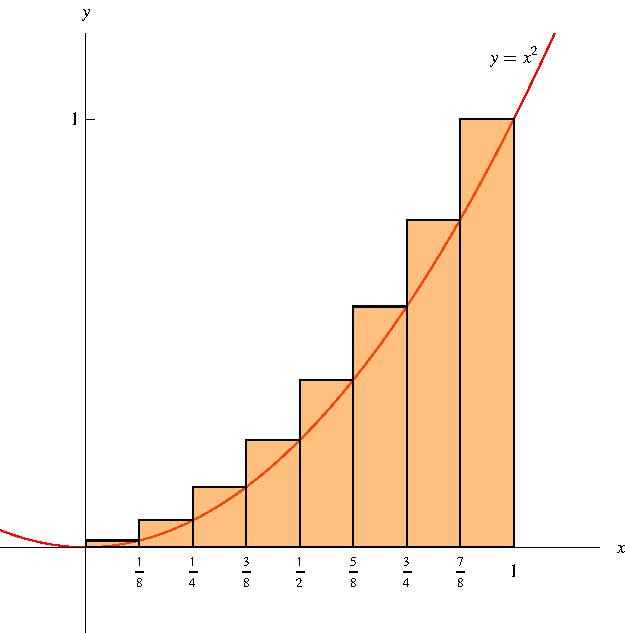
\includegraphics[height=4.5cm]{integration/pictures/05-01-rightd.pdf}%
%}%
%\only<handout:0| 5>{%
%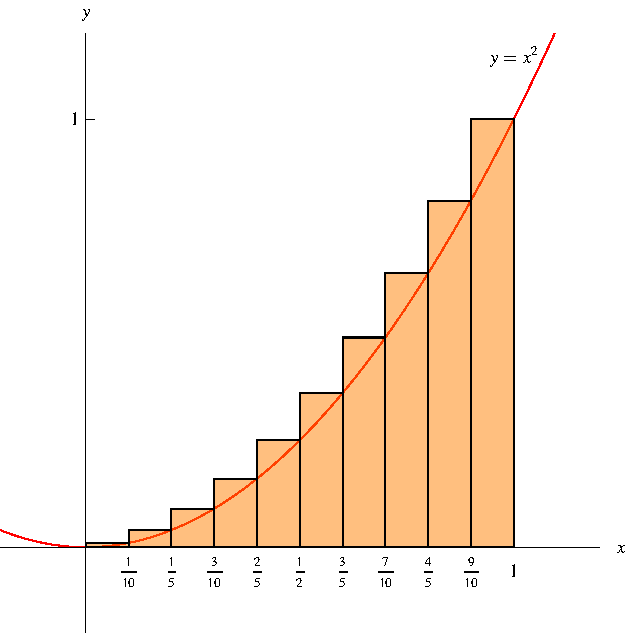
\includegraphics[height=4.5cm]{integration/pictures/05-01-righte.pdf}%
%}%
%\only<handout:0| 6>{%
%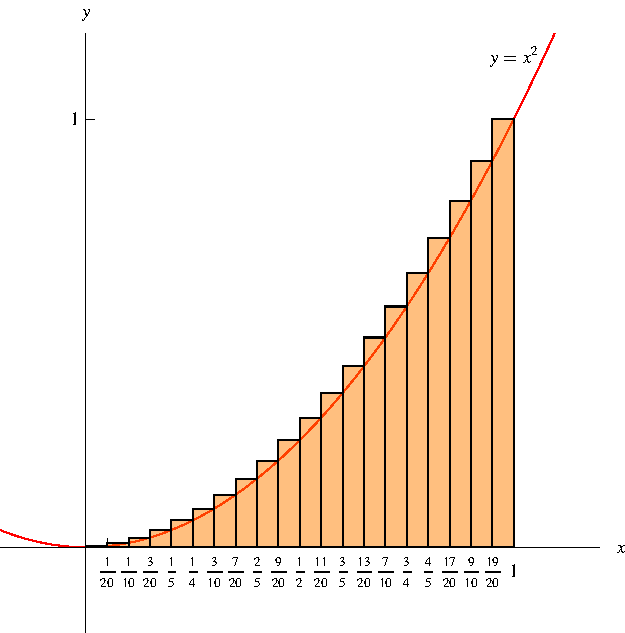
\includegraphics[height=4.5cm]{integration/pictures/05-01-rightf.pdf}%
%}%
%\only<handout:1-| 7>{%
%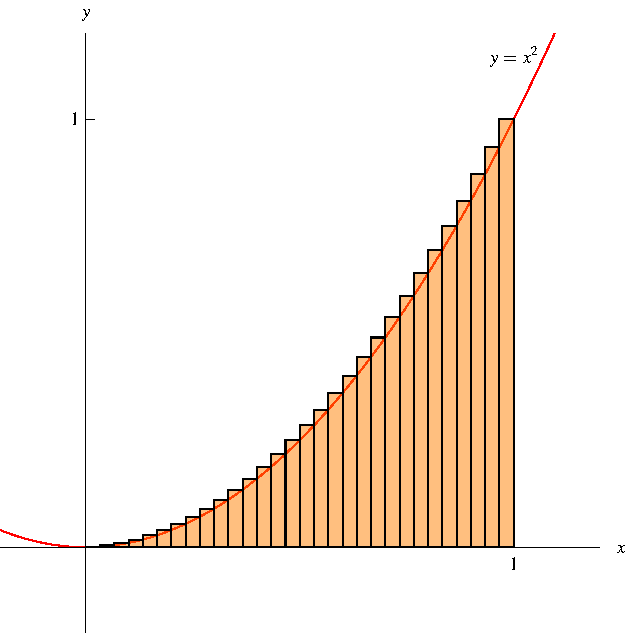
\includegraphics[height=4.5cm]{integration/pictures/05-01-rightg.pdf}%
%}%
%\only<handout:0| 8->{%
%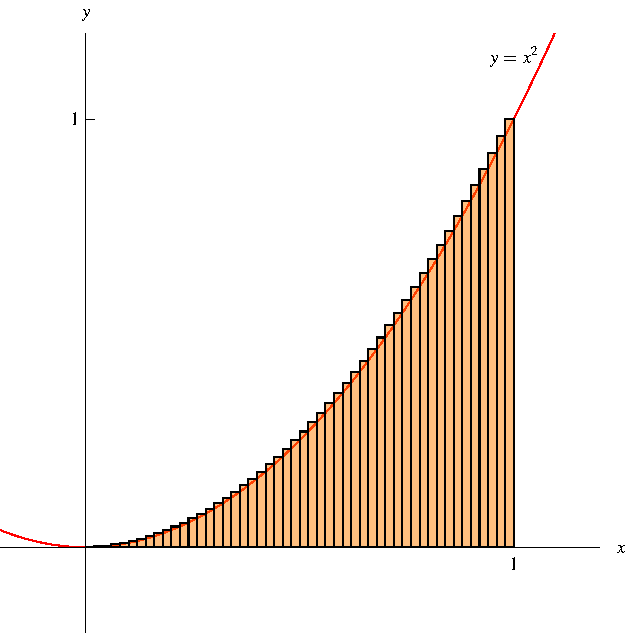
\includegraphics[height=4.5cm]{integration/pictures/05-01-righth.pdf}%
%}%
\end{columns}
\abovedisplayskip=0pt
\belowdisplayskip=0pt
\[
\begin{array}{l}
\uncover<13->{%
\displaystyle R_n  =  \frac{1}{n} \left(\frac{1}{n}\right)^2%
 + \frac{1}{n} \left(\frac{2}{n}\right)^2%
 + \cdots%
 + \frac{1}{n} \left( \frac{n}{n}\right)^2%
}%
\uncover<14->{%
 = \frac{1}{n^3} \alert<handout:0| 15-17>{\left( 1^2 + 2^2 + \cdots + n^2\right)}%
}%
\\%
\uncover<17->{%
\displaystyle \lim_{n\to\infty}R_n  =  \lim_{n\to\infty}\frac{1}{n^3}%
 \alert<handout:0| 17>{\frac{n(n+1)(2n+1)}{6}}%
}%
\uncover<18->{%
 = \lim_{n\to\infty} \frac{1}{\alert<handout:0| 19>{6}} \left( 1 + \frac{1}{n}\right)\left( \alert<handout:0| 19>{2} + \frac{1}{n}\right)%
}%
\uncover<19->{%
 = \alert<handout:0| 19>{\frac{1}{3}}%
}%
\end{array}
\]
\end{example}
\end{frame}
% end module areas-ex2

% begin module area-def
\begin{frame}
Estimate the area under the curve $y = f(x)$ between $a$ and $b$.
\begin{columns}
\column{.55\textwidth}
\psset{xunit=3cm, yunit=3cm}
\begin{pspicture}(-5, -5)(5,5)
\psframe*[linecolor=white](-5,-5)(5,5)
\psaxes[ticks=none, labels=none]{<->}(0,0)(-0.1,-0.1)(1.7,0.9)
\tiny

\uncover<1>{
\psline*[linecolor=\fcColorAreaUnderGraph, linewidth=0.1pt](0.425, 0)(0.425, 0.339931)(0.3, 0.339931)(0.3, 0)(0.55, 0)(0.55, 0.316508)(0.425, 0.316508)(0.425, 0)(0.675, 0)(0.675, 0.348456)(0.55, 0.348456)(0.55, 0)(0.8, 0)(0.8, 0.416)(0.675, 0.416)(0.675, 0)(0.925, 0)(0.925, 0.499364)(0.8, 0.499364)(0.8, 0)(1.05, 0)(1.05, 0.578773)(0.925, 0.578773)(0.925, 0)(1.175, 0)(1.175, 0.634452)(1.05, 0.634452)(1.05, 0)(1.3, 0)(1.3, 0.646625)(1.175, 0.646625)(1.175, 0)(1.425, 0)(1.425, 0.595517)(1.3, 0.595517)(1.3, 0)(1.55, 0)(1.55, 0.461352)(1.425, 0.461352)(1.425, 0)
\psline[linecolor=blue, linewidth=0.1pt](0.425, 0)(0.425, 0.339931)(0.3, 0.339931)(0.3, 0)(0.55, 0)(0.55, 0.316508)(0.425, 0.316508)(0.425, 0)(0.675, 0)(0.675, 0.348456)(0.55, 0.348456)(0.55, 0)(0.8, 0)(0.8, 0.416)(0.675, 0.416)(0.675, 0)(0.925, 0)(0.925, 0.499364)(0.8, 0.499364)(0.8, 0)(1.05, 0)(1.05, 0.578773)(0.925, 0.578773)(0.925, 0)(1.175, 0)(1.175, 0.634452)(1.05, 0.634452)(1.05, 0)(1.3, 0)(1.3, 0.646625)(1.175, 0.646625)(1.175, 0)(1.425, 0)(1.425, 0.595517)(1.3, 0.595517)(1.3, 0)(1.55, 0)(1.55, 0.461352)(1.425, 0.461352)(1.425, 0)
}
\uncover<2->{
\psline*[linecolor=\fcColorAreaUnderGraph, linewidth=0.1pt](0.3, 0)(0.3, 0.4385)(0.425, 0.4385)(0.425, 0)(0.425, 0)(0.425, 0.339931)(0.55, 0.339931)(0.55, 0)(0.55, 0)(0.55, 0.316508)(0.675, 0.316508)(0.675, 0)(0.675, 0)(0.675, 0.348456)(0.8, 0.348456)(0.8, 0)(0.8, 0)(0.8, 0.416)(0.925, 0.416)(0.925, 0)(0.925, 0)(0.925, 0.499364)(1.05, 0.499364)(1.05, 0)(1.05, 0)(1.05, 0.578773)(1.175, 0.578773)(1.175, 0)(1.175, 0)(1.175, 0.634452)(1.3, 0.634452)(1.3, 0)(1.3, 0)(1.3, 0.646625)(1.425, 0.646625)(1.425, 0)(1.425, 0)(1.425, 0.595517)(1.55, 0.595517)(1.55, 0)
\psline[linecolor=blue, linewidth=0.1pt](0.3, 0)(0.3, 0.4385)(0.425, 0.4385)(0.425, 0)(0.425, 0)(0.425, 0.339931)(0.55, 0.339931)(0.55, 0)(0.55, 0)(0.55, 0.316508)(0.675, 0.316508)(0.675, 0)(0.675, 0)(0.675, 0.348456)(0.8, 0.348456)(0.8, 0)(0.8, 0)(0.8, 0.416)(0.925, 0.416)(0.925, 0)(0.925, 0)(0.925, 0.499364)(1.05, 0.499364)(1.05, 0)(1.05, 0)(1.05, 0.578773)(1.175, 0.578773)(1.175, 0)(1.175, 0)(1.175, 0.634452)(1.3, 0.634452)(1.3, 0)(1.3, 0)(1.3, 0.646625)(1.425, 0.646625)(1.425, 0)(1.425, 0)(1.425, 0.595517)(1.55, 0.595517)(1.55, 0)
}
\rput[t](0.3,-0.03){$a$}
\rput[t](0.425,-0.03){$x_1$}
\rput[t](0.55,-0.03){$x_2$}
%\rput[t](0.675,-0.03){}
%\rput[t](0.8,-0.03){$\frac{4}{5}$}
\rput[t](0.7375,-0.06){$\dots$}
\rput[t](0.925,-0.03){$x_{i-1}$}
\rput[t](1.05,-0.03){$x_{i}$}
%\rput[t](1.175,-0.03){$x_i$}
%\rput[t](1.3,-0.03){$\frac{13}{10}$}
\rput[t](1.3,-0.06){$\dots$}
%\rput[t](1.425,-0.03){$\frac{57}{40}$}
\rput[t](1.55,-0.03){$b$}
%Function formula: -171/50 (x)-27/16 ((x)^{3})+11/10+729/160 ((x)^{2})
\psplot[linecolor=red, plotpoints=1000]{0.3}{1.55}{x 2 exp 4.55625 mul 1.1 add x 3 exp -1.6875 mul add x -3.42 mul add }
\psline{<->}(1.6,0)(1.6, 0.578773)
\psline[linestyle=dotted](1.6, 0.578773)(1.05, 0.578773)
\rput[l](1.6, 0.3343865){$f(x_i)$}
\rput[b](0.9875,0.70773){$\Delta x$}
\psline(0.925,0.668773)(1.05, 0.668773)
\psline(0.925,0.648773)(0.925,0.688773)
\psline(1.05, 0.648773)(1.05, 0.688773)

%\psbrace[linecolor=red,ref=lC](2)(3){Text I}
%\uput{:U}{$\overbrace{}^\text{\normalsize A line}$}
\end{pspicture}
%\only<handout:1| -1>{%
%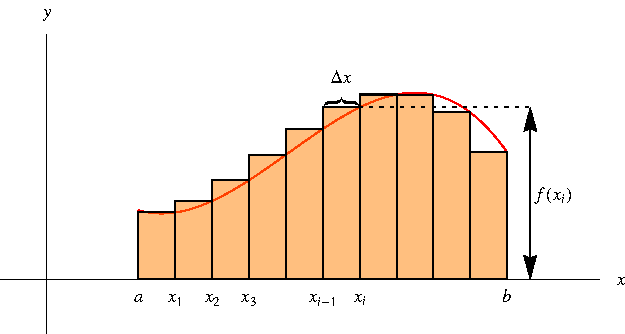
\includegraphics[height=3.5cm]{integration/pictures/05-01-rectangles-right.pdf}%
%}%
%\only<handout:2| 2->{%
%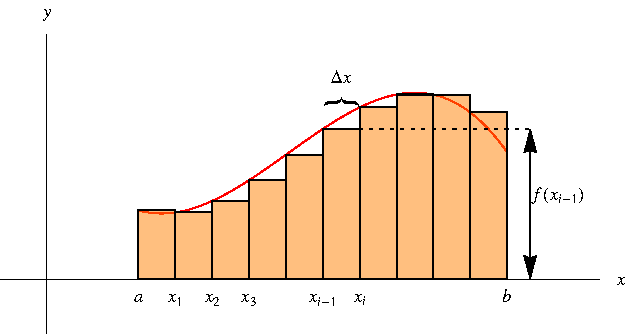
\includegraphics[height=3.5cm]{integration/pictures/05-01-rectangles-left.pdf}%
%}%



\begin{itemize}
\item<1->  Width of whole interval is $b-a$.
\item<1->  $n$ strips, each with width $\Delta x = \frac{b-a}{n}$.
\item<1->  Strips divide $[a,b]$ into $n$ subintervals:\\ $[x_0, x_1]$, $[x_1,x_2]$, $\ldots ,$ $[x_{n-1},x_n]$,\\ where $x_0 = a$ and $x_n = b$.
\end{itemize}
\column{.45\textwidth}
\begin{itemize}
\item<1->  The \only<handout:1| -1>{right}\only<handout:2| 2->{\alert<handout:2| 2>{left}} endpoints of the subintervals are
\end{itemize}
\abovedisplayskip=0pt
\belowdisplayskip=0pt
\begin{eqnarray*}
x_{\only<handout:1| -1>{1}\only<handout:2| 2->{\alert<handout:2| 2>{0}}} & = & a \only<handout:1| -1>{+ \Delta x}\\
x_{\only<handout:1| -1>{2}\only<handout:2| 2->{\alert<handout:2| 2>{1}}} & = & a + \only<handout:1| -1>{2}\Delta x\\
x_{\only<handout:1| -1>{3}\only<handout:2| 2->{\alert<handout:2| 2>{2}}} & = & a + \only<handout:1| -1>{3}\only<handout:2| 2->{2}\Delta x\\
& \vdots &
\end{eqnarray*}
\begin{itemize}
\item<1->  The height of the $i$th rectangle is $f(x_{i\only<handout:2| 2->{\alert<handout:2| 2>{-1}}})$.
\item<1->  The area of the $i$th rectangle is $f(x_{i\only<handout:2| 2->{\alert<handout:2| 2>{-1}}})\Delta x$.
\end{itemize}
\end{columns}
\abovedisplayskip=0pt
\belowdisplayskip=0pt
\[
\only<handout:1| -1>{R_n}\only<handout:2| 2->{\alert<handout:2| 2>{L_n}} = f(x_{\only<handout:1| -1>{1}\only<handout:2| 2->{\alert<handout:2| 2>{0}}})\Delta x + f(x_{\only<handout:1| -1>{2}\only<handout:2| 2->{\alert<handout:2| 2>{1}}})\Delta x + f(x_{\only<handout:1| -1>{3}\only<handout:2| 2->{\alert<handout:2| 2>{2}}})\Delta x + \cdots + f(x_{n\only<handout:2| 2->{\alert<handout:2| 2>{-1}}})\Delta x
\]
\end{frame}

\begin{frame}
\begin{definition}[Area Under a Non-negative Curve]
If $ f\ge 0 $ on $[a,b]$, then the area  under the curve $y = f(x)$ between $ x=a $ and $ x=b  $ is defined to be the limit of the sum of the areas of the approximating rectangles, if that limit exists:
\abovedisplayskip=0pt
\belowdisplayskip=0pt
\[
A = \lim_{n\to\infty} R_n = \lim_{n\to\infty}\sum_{i=1}^n f(x_i)\Delta x
\]
where $ \Delta x =\frac{b-a}{n} $, and $ x_i=a+i\Delta x $.
\end{definition}
\begin{itemize}
\item<2->  This limit always exists if $f$ is continuous.
\item<3->  If $f$ is continuous, we get the same limit if we use left endpoints:
\abovedisplayskip=0pt
\belowdisplayskip=0pt
\[
A = \lim_{n\to\infty} L_n = \lim_{n\to\infty}\sum_{i=1}^n f(x_{i-1})\Delta x = \lim_{n\to\infty}\sum_{i=0}^{n-1} f(x_i)\Delta x
\]
\item<4->  If $f$ is continuous, we get the same limit if we use any number $x_i^*$ in the interval $[x_{i-1},x_i]$.  $x_i^*$ is called a sample point.
\abovedisplayskip=0pt
\belowdisplayskip=0pt
\[
A = \lim_{n\to\infty}\sum_{i=1}^n f(x_i^*)\Delta x
\]

\url{http://www.calculusapplets.com/riemann.html}

\end{itemize}

\end{frame}
% end module area-def

%% begin module sigma-notation
\begin{frame}
\[
\mathop{\alert<handout:0| 2>{\sum}}_{\alert<handout:0| 3>{i=1}}^{\alert<handout:0| 4>{n}} f(x_i)\Delta x = f(x_1)\Delta x + f(x_2)\Delta x + \cdots + f(x_n)\Delta x
\]
\begin{itemize}
\item  We use sigma notation to write sums more compactly.
\item<2-| alert@2>  $\sum$ is the Greek letter sigma.  It tells us to add.
\item<3-| alert@3>  The subscript tells us to start at 1.
\item<4-| alert@4>  The superscript tells us to finish at $n$.
\end{itemize}
\uncover<5->{%
\begin{example}
\begin{eqnarray*}
\sum_{i=1}^4 2i\Delta x & = & 2\Delta x + 4 \Delta x + 6 \Delta x + 8\Delta x\\
\uncover<6->{\alert<handout:0| 6-7>{\sum_{i=3}^7 i^2\Delta x}} & \uncover<6->{\alert<handout:0| 6-7>{=}} & \uncover<7->{\alert<handout:0| 7>{9\Delta x + 16 \Delta x + 25 \Delta x + 36\Delta x + 49\Delta x}}
\end{eqnarray*}
\end{example}
}%
\end{frame}
% end module sigma-notation

\section{The Definite Integral}
% begin module definite-integral-def
\begin{frame}\frametitle{ %(5.2) 
The Definite Integral}
\begin{definition}[Definite Integral]
\begin{itemize}
\item  Let $f:[a,b]\to {\mathbb{R}}$.
\item  Divide $[a,b]$ into $n$ subintervals of equal width $\Delta x = (b-a)/n$.
\item  Let $a=x_0$, $x_1,\ldots ,$ $x_n=b $ be the endpoints of the subintervals, so $ x_i=a+i\Delta x $ .
\item  Let $x_1^*, x_2^*, \ldots , x_n^*$ be any sample points, $x_i^*\in [x_{i-1},x_i]$.  
\end{itemize}
\pause 
\abovedisplayskip=0pt
\belowdisplayskip=0pt
If the limit \[\lim\limits_{n\to \infty} \sum\limits_{i=1}^n f(x_i^*)\Delta x\] 
exists and is independent of the choice of sample points $x_i^*$, then we say $ f $ is \textbf{integrable} on [a,b], and we call this limit \textbf{the integral} of $f$ over $[a,b]$ and write
\[
\int_a^b f(x) \diff x = \lim_{n\to \infty} \sum_{i=1}^n f(x_i^*)\Delta x \quad .
\]
\end{definition}
\end{frame}

\begin{frame}
\begin{definition}[Definite Integral Cont'd: Sample points may be chosen in many ways]
%\[
%\int_a^b f(x) \diff x = \lim_{n\to \infty} \sum_{i=1}^n f(x_i^*)\Delta x \quad .
%\] \pause
Using the right hand approximation, $ x_i^*=x_i $, so we would have 
\[
\int_a^b{f(x)}  \diff x = \lim_{n\to \infty} R_n  = \lim_{n\to \infty} \sum_{i=1}^n f(x_i)\Delta x,
\]\pause
using the left hand approximation, $ x_i^*=x_{i-1} $, so we would have 
\[
\int_a^b{f(x)}  \diff x = \lim_{n\to \infty} L_n  = \lim_{n\to \infty} \sum_{i=1}^n f(x_{i-1})\Delta x,
\]
\pause
choosing $ x_i^*$ to be the midpoint of the interval $ =\overline{x}_i=\frac{1}{2}(x_{i-1}+x_i)$  we have
\[
\int_a^b f(x)\diff x =\lim_{n\to \infty}M_n=\lim_{n\to \infty} \sum_{i=1}^n f(\overline{x}_i)\Delta x
\]

\end{definition}
\end{frame}

\begin{frame}{Notation/Terminology of the definite integral}
\[
\mathop{\alert<handout:0| 2>{\int}}_{\alert<handout:0| 4>{a}}^{\alert<handout:0| 4>{b}} \alert<handout:0| 3>{f(x)} \alert<handout:0| 0>{\diff x} = \lim_{n\to \infty} \sum_{i=1}^n f(x_i^*)\Delta x,
\]
\begin{itemize}
\item<1-| alert@2>  $\int$ is called the integration sign.
\item<1-| alert@3>  $f(x)$ is called the integrand.
\item<1-| alert@4>  $a$ and $b$ are called the limits of integration.
\item<5->  The definite integral is a number.  It does not depend on $x$.  We could use any variable instead of $x$.
\end{itemize}
\uncover<5->{%
\[
\int_a^b f(x) \diff x = \int_a^b f(t)\diff t = \int_a^b f(r)\diff r = \int_a^b f(\theta )\diff \theta
\]
}%

\uncover<6->{\begin{definition}[Riemann Sum]
A Riemann sum is any sum of the form
\abovedisplayskip=0pt
\belowdisplayskip=0pt
\[
\sum_{i=1}^nf(x_i^*) \Delta x = f(x_1^*)\Delta x + f(x_2^*) \Delta x + \cdots + f(x_{n}^*) \Delta x.
\]
\end{definition}
}
\end{frame}
% end module definite-integral-def

%% begin module midpoint-rule
\begin{frame}
\frametitle{The Midpoint Rule}
\begin{itemize}
\item  We've learned that any sample point $x_i^*$ in $[x_{i-1},x_i]$ will work.
\item  However, choosing $x_i^*$ to be the midpoint of the interval often gives the best approximation.
\item  This midpoint is denoted by $\overline{x}_i$.
\end{itemize}
The Midpoint Rule says
\[
\int_a^b f(x)\diff x \approx \sum_{i=1}^n f(\overline{x}_i)\Delta x
\]
where
\[
\Delta x = \frac{b-a}{n}
\]
and
\[
\overline{x}_i=\frac{1}{2}(x_{i-1}+x_i).
\]
\end{frame}
% end module midpoint-rule

% begin module continuous-functions-integrable
\begin{frame}
\begin{theorem}
Let $f$ be a continuous function on $[a,b]$. Then $f$ is integrable over $[a,b]$.
\end{theorem}
\begin{itemize}
\item In particular the integral does not depend the choice of sampling points so long as the intervals containing them shrink.
\item The proof of this theorem is not difficult, but is outside of the scope of Calculus I and II.
\item The only ``difficulty'' in the proof stems from the fact that we have not rigorously constructed the real numbers. 
\item We already (silently) assumed a construction of the real numbers when we defined limits. 
\item Such a construction is also (silently) assumed in most regular high school mathematics courses.
%\item  The proof of the Theorem uses the fact that every set bounded above has a least upper bound. The latter fact is either taken as an axiom of the real numbers, or is proven from equivalent set of axioms. This is the main fact a calculus student is missing to understand/prove on one's own the above theorem.
\item A student interested in a proof of the theorem should google ``Darboux integral''.
\end{itemize}

\end{frame}
% end module continuous-functions-integrable

% begin module definite-integral-negative
\begin{frame}
\begin{columns}
\column{.55\textwidth}
\begin{itemize}
\item  We know already that if $f(x)$ is always positive, then $\int_a^bf(x)\diff x$ is the area under the curve.
\end{itemize}
\column{.45\textwidth}
\psset{xunit=2cm, yunit=2cm}
\begin{pspicture}(-0.15,-0.15)(1.5,1.5)
\psline{linecolor=red!1}(0, -0.3)(0, -0.31)
\psframe*[linecolor=white](-0.15,-0.15)(1.5,1.5)
\tiny
\psline(-0.05, 1)(0.05,1)
\rput[r] (-0.07,1){$1$}
%Function formula: x^{2}
\rput(0.9,1.3){$y=x^{2}$}
\uncover<handout:0|1>{
%approximation 1/3
\psline*[linecolor=\fcColorAreaUnderGraph, linewidth=0.1pt](0.333333, 0)(0.333333, 0.111111)(0, 0.111111)(0, 0)(0.666667, 0)(0.666667, 0.444444)(0.333333, 0.444444)(0.333333, 0)(1, 0)(1, 1)(0.666667, 1)(0.666667, 0)
\psline[linecolor=blue, linewidth=0.1pt](0.333333, 0)(0.333333, 0.111111)(0, 0.111111)(0, 0)(0.666667, 0)(0.666667, 0.444444)(0.333333, 0.444444)(0.333333, 0)(1, 0)(1, 1)(0.666667, 1)(0.666667, 0)
\rput[t](0.333333,-0.03){$\frac{1}{3}$}\rput[t](0.666667,-0.03){$\frac{2}{3}$}\rput[t](1,-0.03){$1$}
}
\uncover<handout:0|2>{
%approximation 1/4
\psline*[linecolor=\fcColorAreaUnderGraph, linewidth=0.1pt](0.25, 0)(0.25, 0.0625)(0, 0.0625)(0, 0)(0.5, 0)(0.5, 0.25)(0.25, 0.25)(0.25, 0)(0.75, 0)(0.75, 0.5625)(0.5, 0.5625)(0.5, 0)(1, 0)(1, 1)(0.75, 1)(0.75, 0)
\psline[linecolor=blue, linewidth=0.1pt](0.25, 0)(0.25, 0.0625)(0, 0.0625)(0, 0)(0.5, 0)(0.5, 0.25)(0.25, 0.25)(0.25, 0)(0.75, 0)(0.75, 0.5625)(0.5, 0.5625)(0.5, 0)(1, 0)(1, 1)(0.75, 1)(0.75, 0)
\rput[t](0.25,-0.03){$\frac{1}{4}$}\rput[t](0.5,-0.03){$\frac{1}{2}$}\rput[t](0.75,-0.03){$\frac{3}{4}$}\rput[t](1,-0.03){$1$}
}
\uncover<handout:0|3>{
%approximation 1/5
\psline*[linecolor=\fcColorAreaUnderGraph, linewidth=0.1pt](0.2, 0)(0.2, 0.04)(0, 0.04)(0, 0)(0.4, 0)(0.4, 0.16)(0.2, 0.16)(0.2, 0)(0.6, 0)(0.6, 0.36)(0.4, 0.36)(0.4, 0)(0.8, 0)(0.8, 0.64)(0.6, 0.64)(0.6, 0)(1, 0)(1, 1)(0.8, 1)(0.8, 0)
\psline[linecolor=blue, linewidth=0.1pt](0.2, 0)(0.2, 0.04)(0, 0.04)(0, 0)(0.4, 0)(0.4, 0.16)(0.2, 0.16)(0.2, 0)(0.6, 0)(0.6, 0.36)(0.4, 0.36)(0.4, 0)(0.8, 0)(0.8, 0.64)(0.6, 0.64)(0.6, 0)(1, 0)(1, 1)(0.8, 1)(0.8, 0)
\rput[t](0.2,-0.03){$\frac{1}{5}$}\rput[t](0.4,-0.03){$\frac{2}{5}$}\rput[t](0.6,-0.03){$\frac{3}{5}$}\rput[t](0.8,-0.03){$\frac{4}{5}$}\rput[t](1,-0.03){$1$}
}
\uncover<handout:0|4>{
%approximation 1/8
\psline*[linecolor=\fcColorAreaUnderGraph, linewidth=0.1pt](0.125, 0)(0.125, 0.015625)(0, 0.015625)(0, 0)(0.25, 0)(0.25, 0.0625)(0.125, 0.0625)(0.125, 0)(0.375, 0)(0.375, 0.140625)(0.25, 0.140625)(0.25, 0)(0.5, 0)(0.5, 0.25)(0.375, 0.25)(0.375, 0)(0.625, 0)(0.625, 0.390625)(0.5, 0.390625)(0.5, 0)(0.75, 0)(0.75, 0.5625)(0.625, 0.5625)(0.625, 0)(0.875, 0)(0.875, 0.765625)(0.75, 0.765625)(0.75, 0)(1, 0)(1, 1)(0.875, 1)(0.875, 0)
\psline[linecolor=blue, linewidth=0.1pt](0.125, 0)(0.125, 0.015625)(0, 0.015625)(0, 0)(0.25, 0)(0.25, 0.0625)(0.125, 0.0625)(0.125, 0)(0.375, 0)(0.375, 0.140625)(0.25, 0.140625)(0.25, 0)(0.5, 0)(0.5, 0.25)(0.375, 0.25)(0.375, 0)(0.625, 0)(0.625, 0.390625)(0.5, 0.390625)(0.5, 0)(0.75, 0)(0.75, 0.5625)(0.625, 0.5625)(0.625, 0)(0.875, 0)(0.875, 0.765625)(0.75, 0.765625)(0.75, 0)(1, 0)(1, 1)(0.875, 1)(0.875, 0)
\rput[t](0.125,-0.03){$\frac{1}{8}$}\rput[t](0.25,-0.03){$\frac{1}{4}$}\rput[t](0.375,-0.03){$\frac{3}{8}$}\rput[t](0.5,-0.03){$\frac{1}{2}$}\rput[t](0.625,-0.03){$\frac{5}{8}$}\rput[t](0.75,-0.03){$\frac{3}{4}$}\rput[t](0.875,-0.03){$\frac{7}{8}$}\rput[t](1,-0.03){$1$}
}
\uncover<handout:0|5>{
%approximation 1/10
\psline*[linecolor=\fcColorAreaUnderGraph, linewidth=0.1pt](0.1, 0)(0.1, 0.01)(0, 0.01)(0, 0)(0.2, 0)(0.2, 0.04)(0.1, 0.04)(0.1, 0)(0.3, 0)(0.3, 0.09)(0.2, 0.09)(0.2, 0)(0.4, 0)(0.4, 0.16)(0.3, 0.16)(0.3, 0)(0.5, 0)(0.5, 0.25)(0.4, 0.25)(0.4, 0)(0.6, 0)(0.6, 0.36)(0.5, 0.36)(0.5, 0)(0.7, 0)(0.7, 0.49)(0.6, 0.49)(0.6, 0)(0.8, 0)(0.8, 0.64)(0.7, 0.64)(0.7, 0)(0.9, 0)(0.9, 0.81)(0.8, 0.81)(0.8, 0)(1, 0)(1, 1)(0.9, 1)(0.9, 0)
\psline[linecolor=blue, linewidth=0.1pt](0.1, 0)(0.1, 0.01)(0, 0.01)(0, 0)(0.2, 0)(0.2, 0.04)(0.1, 0.04)(0.1, 0)(0.3, 0)(0.3, 0.09)(0.2, 0.09)(0.2, 0)(0.4, 0)(0.4, 0.16)(0.3, 0.16)(0.3, 0)(0.5, 0)(0.5, 0.25)(0.4, 0.25)(0.4, 0)(0.6, 0)(0.6, 0.36)(0.5, 0.36)(0.5, 0)(0.7, 0)(0.7, 0.49)(0.6, 0.49)(0.6, 0)(0.8, 0)(0.8, 0.64)(0.7, 0.64)(0.7, 0)(0.9, 0)(0.9, 0.81)(0.8, 0.81)(0.8, 0)(1, 0)(1, 1)(0.9, 1)(0.9, 0)
\rput[t](0.1,-0.03){$\frac{1}{10}$}\rput[t](0.2,-0.03){$\frac{1}{5}$}\rput[t](0.3,-0.03){$\frac{3}{10}$}\rput[t](0.4,-0.03){$\frac{2}{5}$}\rput[t](0.5,-0.03){$\frac{1}{2}$}\rput[t](0.6,-0.03){$\frac{3}{5}$}\rput[t](0.7,-0.03){$\frac{7}{10}$}\rput[t](0.8,-0.03){$\frac{4}{5}$}\rput[t](0.9,-0.03){$\frac{9}{10}$}\rput[t](1,-0.03){$1$}
}
\uncover<handout:1|6>{
%approximation 1/20
\psline*[linecolor=\fcColorAreaUnderGraph, linewidth=0.1pt](0.05, 0)(0.05, 0.0025)(0, 0.0025)(0, 0)(0.1, 0)(0.1, 0.01)(0.05, 0.01)(0.05, 0)(0.15, 0)(0.15, 0.0225)(0.1, 0.0225)(0.1, 0)(0.2, 0)(0.2, 0.04)(0.15, 0.04)(0.15, 0)(0.25, 0)(0.25, 0.0625)(0.2, 0.0625)(0.2, 0)(0.3, 0)(0.3, 0.09)(0.25, 0.09)(0.25, 0)(0.35, 0)(0.35, 0.1225)(0.3, 0.1225)(0.3, 0)(0.4, 0)(0.4, 0.16)(0.35, 0.16)(0.35, 0)(0.45, 0)(0.45, 0.2025)(0.4, 0.2025)(0.4, 0)(0.5, 0)(0.5, 0.25)(0.45, 0.25)(0.45, 0)(0.55, 0)(0.55, 0.3025)(0.5, 0.3025)(0.5, 0)(0.6, 0)(0.6, 0.36)(0.55, 0.36)(0.55, 0)(0.65, 0)(0.65, 0.4225)(0.6, 0.4225)(0.6, 0)(0.7, 0)(0.7, 0.49)(0.65, 0.49)(0.65, 0)(0.75, 0)(0.75, 0.5625)(0.7, 0.5625)(0.7, 0)(0.8, 0)(0.8, 0.64)(0.75, 0.64)(0.75, 0)(0.85, 0)(0.85, 0.7225)(0.8, 0.7225)(0.8, 0)(0.9, 0)(0.9, 0.81)(0.85, 0.81)(0.85, 0)(0.95, 0)(0.95, 0.9025)(0.9, 0.9025)(0.9, 0)(1, 0)(1, 1)(0.95, 1)(0.95, 0)
\psline[linecolor=blue, linewidth=0.1pt](0.05, 0)(0.05, 0.0025)(0, 0.0025)(0, 0)(0.1, 0)(0.1, 0.01)(0.05, 0.01)(0.05, 0)(0.15, 0)(0.15, 0.0225)(0.1, 0.0225)(0.1, 0)(0.2, 0)(0.2, 0.04)(0.15, 0.04)(0.15, 0)(0.25, 0)(0.25, 0.0625)(0.2, 0.0625)(0.2, 0)(0.3, 0)(0.3, 0.09)(0.25, 0.09)(0.25, 0)(0.35, 0)(0.35, 0.1225)(0.3, 0.1225)(0.3, 0)(0.4, 0)(0.4, 0.16)(0.35, 0.16)(0.35, 0)(0.45, 0)(0.45, 0.2025)(0.4, 0.2025)(0.4, 0)(0.5, 0)(0.5, 0.25)(0.45, 0.25)(0.45, 0)(0.55, 0)(0.55, 0.3025)(0.5, 0.3025)(0.5, 0)(0.6, 0)(0.6, 0.36)(0.55, 0.36)(0.55, 0)(0.65, 0)(0.65, 0.4225)(0.6, 0.4225)(0.6, 0)(0.7, 0)(0.7, 0.49)(0.65, 0.49)(0.65, 0)(0.75, 0)(0.75, 0.5625)(0.7, 0.5625)(0.7, 0)(0.8, 0)(0.8, 0.64)(0.75, 0.64)(0.75, 0)(0.85, 0)(0.85, 0.7225)(0.8, 0.7225)(0.8, 0)(0.9, 0)(0.9, 0.81)(0.85, 0.81)(0.85, 0)(0.95, 0)(0.95, 0.9025)(0.9, 0.9025)(0.9, 0)(1, 0)(1, 1)(0.95, 1)(0.95, 0)
}
\uncover<handout:0|7>{
%approximation 1/30
\psline*[linecolor=\fcColorAreaUnderGraph, linewidth=0.1pt](0.0333333, 0)(0.0333333, 0.00111111)(0, 0.00111111)(0, 0)(0.0666667, 0)(0.0666667, 0.00444444)(0.0333333, 0.00444444)(0.0333333, 0)(0.1, 0)(0.1, 0.01)(0.0666667, 0.01)(0.0666667, 0)(0.133333, 0)(0.133333, 0.0177778)(0.1, 0.0177778)(0.1, 0)(0.166667, 0)(0.166667, 0.0277778)(0.133333, 0.0277778)(0.133333, 0)(0.2, 0)(0.2, 0.04)(0.166667, 0.04)(0.166667, 0)(0.233333, 0)(0.233333, 0.0544444)(0.2, 0.0544444)(0.2, 0)(0.266667, 0)(0.266667, 0.0711111)(0.233333, 0.0711111)(0.233333, 0)(0.3, 0)(0.3, 0.09)(0.266667, 0.09)(0.266667, 0)(0.333333, 0)(0.333333, 0.111111)(0.3, 0.111111)(0.3, 0)(0.366667, 0)(0.366667, 0.134444)(0.333333, 0.134444)(0.333333, 0)(0.4, 0)(0.4, 0.16)(0.366667, 0.16)(0.366667, 0)(0.433333, 0)(0.433333, 0.187778)(0.4, 0.187778)(0.4, 0)(0.466667, 0)(0.466667, 0.217778)(0.433333, 0.217778)(0.433333, 0)(0.5, 0)(0.5, 0.25)(0.466667, 0.25)(0.466667, 0)(0.533333, 0)(0.533333, 0.284444)(0.5, 0.284444)(0.5, 0)(0.566667, 0)(0.566667, 0.321111)(0.533333, 0.321111)(0.533333, 0)(0.6, 0)(0.6, 0.36)(0.566667, 0.36)(0.566667, 0)(0.633333, 0)(0.633333, 0.401111)(0.6, 0.401111)(0.6, 0)(0.666667, 0)(0.666667, 0.444444)(0.633333, 0.444444)(0.633333, 0)(0.7, 0)(0.7, 0.49)(0.666667, 0.49)(0.666667, 0)(0.733333, 0)(0.733333, 0.537778)(0.7, 0.537778)(0.7, 0)(0.766667, 0)(0.766667, 0.587778)(0.733333, 0.587778)(0.733333, 0)(0.8, 0)(0.8, 0.64)(0.766667, 0.64)(0.766667, 0)(0.833333, 0)(0.833333, 0.694444)(0.8, 0.694444)(0.8, 0)(0.866667, 0)(0.866667, 0.751111)(0.833333, 0.751111)(0.833333, 0)(0.9, 0)(0.9, 0.81)(0.866667, 0.81)(0.866667, 0)(0.933333, 0)(0.933333, 0.871111)(0.9, 0.871111)(0.9, 0)(0.966667, 0)(0.966667, 0.934444)(0.933333, 0.934444)(0.933333, 0)(1, 0)(1, 1)(0.966667, 1)(0.966667, 0)
\psline[linecolor=blue, linewidth=0.1pt](0.0333333, 0)(0.0333333, 0.00111111)(0, 0.00111111)(0, 0)(0.0666667, 0)(0.0666667, 0.00444444)(0.0333333, 0.00444444)(0.0333333, 0)(0.1, 0)(0.1, 0.01)(0.0666667, 0.01)(0.0666667, 0)(0.133333, 0)(0.133333, 0.0177778)(0.1, 0.0177778)(0.1, 0)(0.166667, 0)(0.166667, 0.0277778)(0.133333, 0.0277778)(0.133333, 0)(0.2, 0)(0.2, 0.04)(0.166667, 0.04)(0.166667, 0)(0.233333, 0)(0.233333, 0.0544444)(0.2, 0.0544444)(0.2, 0)(0.266667, 0)(0.266667, 0.0711111)(0.233333, 0.0711111)(0.233333, 0)(0.3, 0)(0.3, 0.09)(0.266667, 0.09)(0.266667, 0)(0.333333, 0)(0.333333, 0.111111)(0.3, 0.111111)(0.3, 0)(0.366667, 0)(0.366667, 0.134444)(0.333333, 0.134444)(0.333333, 0)(0.4, 0)(0.4, 0.16)(0.366667, 0.16)(0.366667, 0)(0.433333, 0)(0.433333, 0.187778)(0.4, 0.187778)(0.4, 0)(0.466667, 0)(0.466667, 0.217778)(0.433333, 0.217778)(0.433333, 0)(0.5, 0)(0.5, 0.25)(0.466667, 0.25)(0.466667, 0)(0.533333, 0)(0.533333, 0.284444)(0.5, 0.284444)(0.5, 0)(0.566667, 0)(0.566667, 0.321111)(0.533333, 0.321111)(0.533333, 0)(0.6, 0)(0.6, 0.36)(0.566667, 0.36)(0.566667, 0)(0.633333, 0)(0.633333, 0.401111)(0.6, 0.401111)(0.6, 0)(0.666667, 0)(0.666667, 0.444444)(0.633333, 0.444444)(0.633333, 0)(0.7, 0)(0.7, 0.49)(0.666667, 0.49)(0.666667, 0)(0.733333, 0)(0.733333, 0.537778)(0.7, 0.537778)(0.7, 0)(0.766667, 0)(0.766667, 0.587778)(0.733333, 0.587778)(0.733333, 0)(0.8, 0)(0.8, 0.64)(0.766667, 0.64)(0.766667, 0)(0.833333, 0)(0.833333, 0.694444)(0.8, 0.694444)(0.8, 0)(0.866667, 0)(0.866667, 0.751111)(0.833333, 0.751111)(0.833333, 0)(0.9, 0)(0.9, 0.81)(0.866667, 0.81)(0.866667, 0)(0.933333, 0)(0.933333, 0.871111)(0.9, 0.871111)(0.9, 0)(0.966667, 0)(0.966667, 0.934444)(0.933333, 0.934444)(0.933333, 0)(1, 0)(1, 1)(0.966667, 1)(0.966667, 0)
}
\uncover<handout:0|8>{
%approximation 1/40
\psline*[linecolor=\fcColorAreaUnderGraph, linewidth=0.1pt](0.025, 0)(0.025, 0.000625)(0, 0.000625)(0, 0)(0.05, 0)(0.05, 0.0025)(0.025, 0.0025)(0.025, 0)(0.075, 0)(0.075, 0.005625)(0.05, 0.005625)(0.05, 0)(0.1, 0)(0.1, 0.01)(0.075, 0.01)(0.075, 0)(0.125, 0)(0.125, 0.015625)(0.1, 0.015625)(0.1, 0)(0.15, 0)(0.15, 0.0225)(0.125, 0.0225)(0.125, 0)(0.175, 0)(0.175, 0.030625)(0.15, 0.030625)(0.15, 0)(0.2, 0)(0.2, 0.04)(0.175, 0.04)(0.175, 0)(0.225, 0)(0.225, 0.050625)(0.2, 0.050625)(0.2, 0)(0.25, 0)(0.25, 0.0625)(0.225, 0.0625)(0.225, 0)(0.275, 0)(0.275, 0.075625)(0.25, 0.075625)(0.25, 0)(0.3, 0)(0.3, 0.09)(0.275, 0.09)(0.275, 0)(0.325, 0)(0.325, 0.105625)(0.3, 0.105625)(0.3, 0)(0.35, 0)(0.35, 0.1225)(0.325, 0.1225)(0.325, 0)(0.375, 0)(0.375, 0.140625)(0.35, 0.140625)(0.35, 0)(0.4, 0)(0.4, 0.16)(0.375, 0.16)(0.375, 0)(0.425, 0)(0.425, 0.180625)(0.4, 0.180625)(0.4, 0)(0.45, 0)(0.45, 0.2025)(0.425, 0.2025)(0.425, 0)(0.475, 0)(0.475, 0.225625)(0.45, 0.225625)(0.45, 0)(0.5, 0)(0.5, 0.25)(0.475, 0.25)(0.475, 0)(0.525, 0)(0.525, 0.275625)(0.5, 0.275625)(0.5, 0)(0.55, 0)(0.55, 0.3025)(0.525, 0.3025)(0.525, 0)(0.575, 0)(0.575, 0.330625)(0.55, 0.330625)(0.55, 0)(0.6, 0)(0.6, 0.36)(0.575, 0.36)(0.575, 0)(0.625, 0)(0.625, 0.390625)(0.6, 0.390625)(0.6, 0)(0.65, 0)(0.65, 0.4225)(0.625, 0.4225)(0.625, 0)(0.675, 0)(0.675, 0.455625)(0.65, 0.455625)(0.65, 0)(0.7, 0)(0.7, 0.49)(0.675, 0.49)(0.675, 0)(0.725, 0)(0.725, 0.525625)(0.7, 0.525625)(0.7, 0)(0.75, 0)(0.75, 0.5625)(0.725, 0.5625)(0.725, 0)(0.775, 0)(0.775, 0.600625)(0.75, 0.600625)(0.75, 0)(0.8, 0)(0.8, 0.64)(0.775, 0.64)(0.775, 0)(0.825, 0)(0.825, 0.680625)(0.8, 0.680625)(0.8, 0)(0.85, 0)(0.85, 0.7225)(0.825, 0.7225)(0.825, 0)(0.875, 0)(0.875, 0.765625)(0.85, 0.765625)(0.85, 0)(0.9, 0)(0.9, 0.81)(0.875, 0.81)(0.875, 0)(0.925, 0)(0.925, 0.855625)(0.9, 0.855625)(0.9, 0)(0.95, 0)(0.95, 0.9025)(0.925, 0.9025)(0.925, 0)(0.975, 0)(0.975, 0.950625)(0.95, 0.950625)(0.95, 0)(1, 0)(1, 1)(0.975, 1)(0.975, 0)
\psline[linecolor=blue, linewidth=0.1pt](0.025, 0)(0.025, 0.000625)(0, 0.000625)(0, 0)(0.05, 0)(0.05, 0.0025)(0.025, 0.0025)(0.025, 0)(0.075, 0)(0.075, 0.005625)(0.05, 0.005625)(0.05, 0)(0.1, 0)(0.1, 0.01)(0.075, 0.01)(0.075, 0)(0.125, 0)(0.125, 0.015625)(0.1, 0.015625)(0.1, 0)(0.15, 0)(0.15, 0.0225)(0.125, 0.0225)(0.125, 0)(0.175, 0)(0.175, 0.030625)(0.15, 0.030625)(0.15, 0)(0.2, 0)(0.2, 0.04)(0.175, 0.04)(0.175, 0)(0.225, 0)(0.225, 0.050625)(0.2, 0.050625)(0.2, 0)(0.25, 0)(0.25, 0.0625)(0.225, 0.0625)(0.225, 0)(0.275, 0)(0.275, 0.075625)(0.25, 0.075625)(0.25, 0)(0.3, 0)(0.3, 0.09)(0.275, 0.09)(0.275, 0)(0.325, 0)(0.325, 0.105625)(0.3, 0.105625)(0.3, 0)(0.35, 0)(0.35, 0.1225)(0.325, 0.1225)(0.325, 0)(0.375, 0)(0.375, 0.140625)(0.35, 0.140625)(0.35, 0)(0.4, 0)(0.4, 0.16)(0.375, 0.16)(0.375, 0)(0.425, 0)(0.425, 0.180625)(0.4, 0.180625)(0.4, 0)(0.45, 0)(0.45, 0.2025)(0.425, 0.2025)(0.425, 0)(0.475, 0)(0.475, 0.225625)(0.45, 0.225625)(0.45, 0)(0.5, 0)(0.5, 0.25)(0.475, 0.25)(0.475, 0)(0.525, 0)(0.525, 0.275625)(0.5, 0.275625)(0.5, 0)(0.55, 0)(0.55, 0.3025)(0.525, 0.3025)(0.525, 0)(0.575, 0)(0.575, 0.330625)(0.55, 0.330625)(0.55, 0)(0.6, 0)(0.6, 0.36)(0.575, 0.36)(0.575, 0)(0.625, 0)(0.625, 0.390625)(0.6, 0.390625)(0.6, 0)(0.65, 0)(0.65, 0.4225)(0.625, 0.4225)(0.625, 0)(0.675, 0)(0.675, 0.455625)(0.65, 0.455625)(0.65, 0)(0.7, 0)(0.7, 0.49)(0.675, 0.49)(0.675, 0)(0.725, 0)(0.725, 0.525625)(0.7, 0.525625)(0.7, 0)(0.75, 0)(0.75, 0.5625)(0.725, 0.5625)(0.725, 0)(0.775, 0)(0.775, 0.600625)(0.75, 0.600625)(0.75, 0)(0.8, 0)(0.8, 0.64)(0.775, 0.64)(0.775, 0)(0.825, 0)(0.825, 0.680625)(0.8, 0.680625)(0.8, 0)(0.85, 0)(0.85, 0.7225)(0.825, 0.7225)(0.825, 0)(0.875, 0)(0.875, 0.765625)(0.85, 0.765625)(0.85, 0)(0.9, 0)(0.9, 0.81)(0.875, 0.81)(0.875, 0)(0.925, 0)(0.925, 0.855625)(0.9, 0.855625)(0.9, 0)(0.95, 0)(0.95, 0.9025)(0.925, 0.9025)(0.925, 0)(0.975, 0)(0.975, 0.950625)(0.95, 0.950625)(0.95, 0)(1, 0)(1, 1)(0.975, 1)(0.975, 0)
}
\uncover<handout:2|9->{
\pscustom*[linecolor=\fcColorAreaUnderGraph, linewidth=0.1pt]{\psplot[linecolor=red, plotpoints=1000]{0}{1}{x 2 exp }\psline(1,1)(1,0)}
}
\psline(1,-0.03)(1,0.03)
\uncover<6->{
\rput[t] (1,-0.07){$1$}
}
\psaxes[ticks=none, labels=none]{<->}(0,0)(-0.1,-0.1)(1.4,1.4)
\psplot[linecolor=red, plotpoints=1000]{0}{1.15}{x 2 exp }
\end{pspicture}
%\only<handout:0| -1>{%
%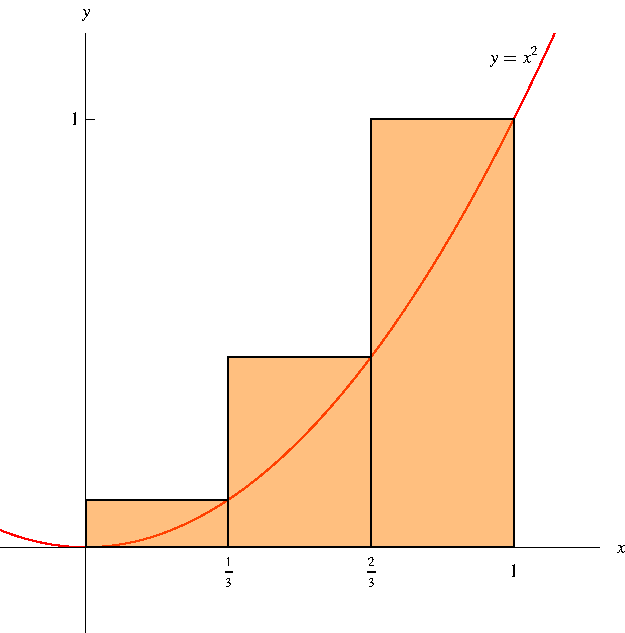
\includegraphics[height=4.2cm]{integration/pictures/05-01-righta.pdf}%
%}%
%\only<handout:0| 2>{%
%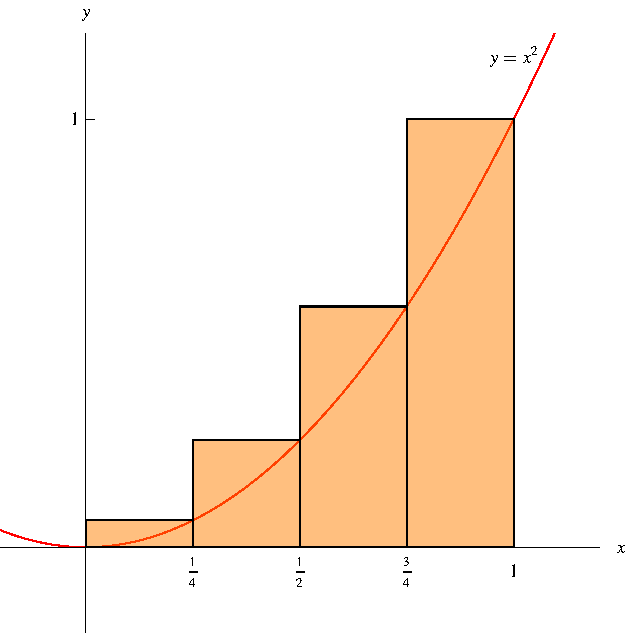
\includegraphics[height=4.2cm]{integration/pictures/05-01-rightb.pdf}%
%}%
%\only<handout:0| 3>{%
%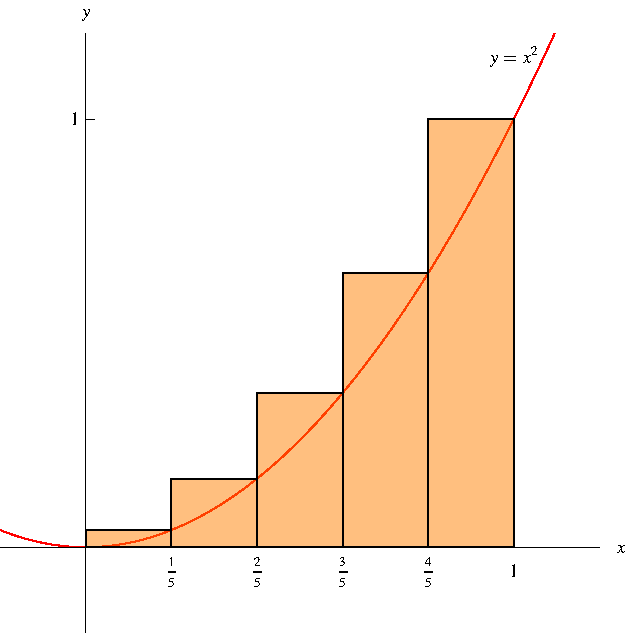
\includegraphics[height=4.2cm]{integration/pictures/05-01-rightc.pdf}%
%}%
%\only<handout:0| 4>{%
%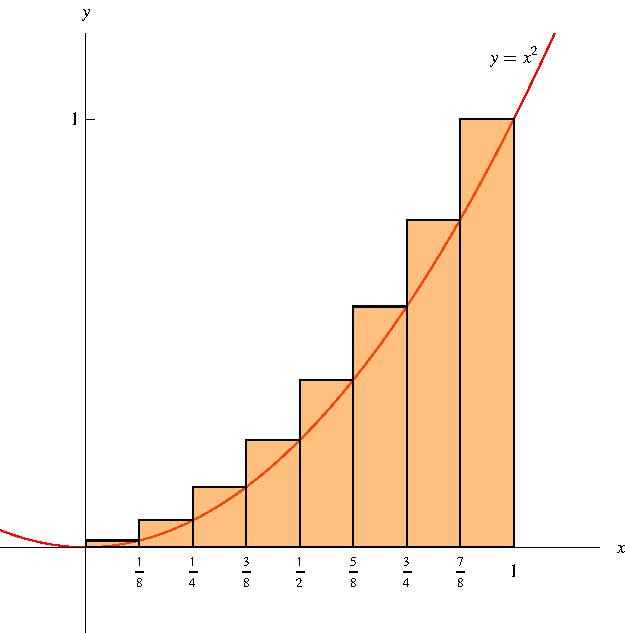
\includegraphics[height=4.2cm]{integration/pictures/05-01-rightd.pdf}%
%}%
%\only<handout:0| 5>{%
%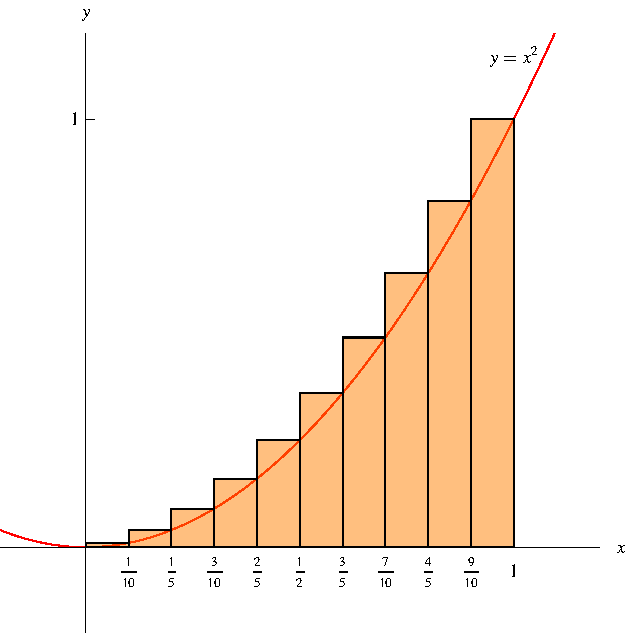
\includegraphics[height=4.2cm]{integration/pictures/05-01-righte.pdf}%
%}%
%\only<handout:0| 6>{%
%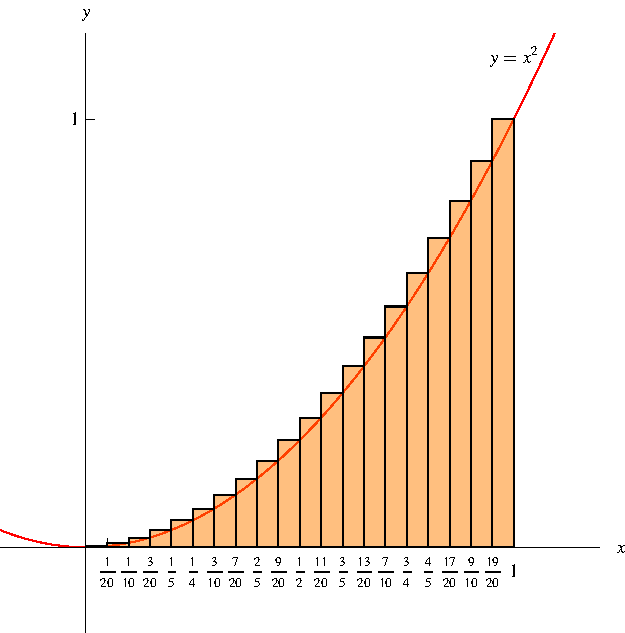
\includegraphics[height=4.2cm]{integration/pictures/05-01-rightf.pdf}%
%}%
%\only<handout:0| 7>{%
%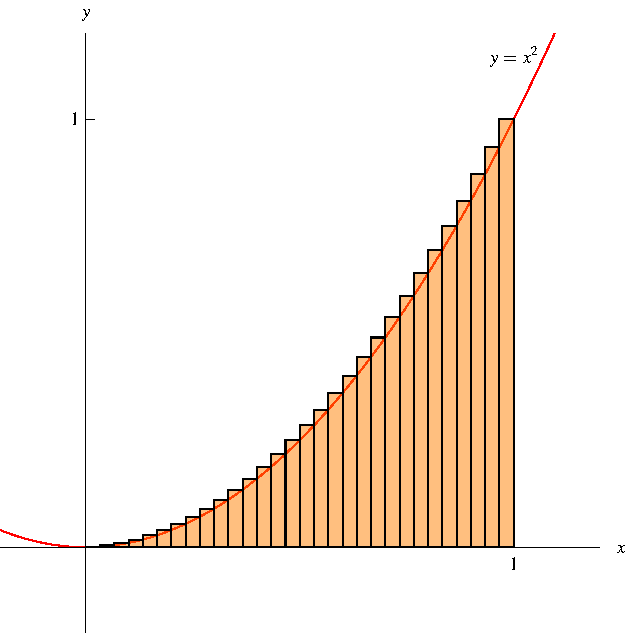
\includegraphics[height=4.2cm]{integration/pictures/05-01-rightg.pdf}%
%}%
%\only<handout:0| 8>{%
%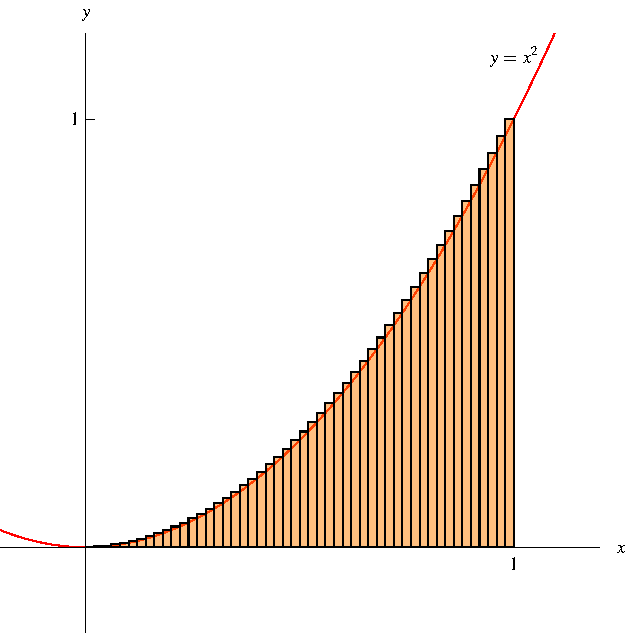
\includegraphics[height=4.2cm]{integration/pictures/05-01-righth.pdf}%
%}%
%\only<handout:1| 9->{%
%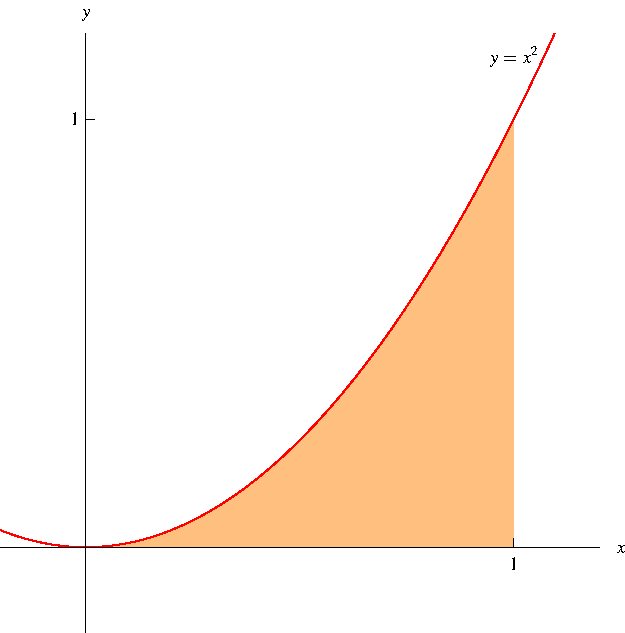
\includegraphics[height=4.2cm]{integration/pictures/05-01-xsquaredarea.pdf}%
%}%
\end{columns}
\begin{columns}
\column{.4\textwidth}


\uncover<10->{%
\psset{xunit=2cm, yunit=2cm}
\begin{pspicture}(-0.15,-1.6)(1.5,1.4)
\psframe*[linecolor=white](-0.15,-1.6)(1.5,1.4)
\tiny
\rput (1, 0.8){$y=f(x)$}
\uncover<handout:0|11>{
\psline*[linecolor=\fcColorNegativeAreaUnderGraph, linewidth=0.1pt](0.45, 0)(0.45, -0.582187)(0.1, -0.582187)(0.1, 0)
\psline*[linecolor=\fcColorAreaUnderGraph, linewidth=0.1pt](0.8, 0)(0.8, 0.512)(0.45, 0.512)(0.45, 0)(1.15, 0)(1.15, 0.142313)(0.8, 0.142313)(0.8, 0)
\psline*[linecolor=\fcColorNegativeAreaUnderGraph, linewidth=0.1pt](1.5, 0)(1.5, -0.405)(1.15, -0.405)(1.15, 0)
\psline[linecolor=brown, linewidth=0.1pt](0.45, 0)(0.45, -0.582187)(0.1, -0.582187)(0.1, 0)
\psline[linecolor=blue, linewidth=0.1pt](0.8, 0)(0.8, 0.512)(0.45, 0.512)(0.45, 0)(1.15, 0)(1.15, 0.142313)(0.8, 0.142313)(0.8, 0)
\psline[linecolor=brown, linewidth=0.1pt](1.5, 0)(1.5, -0.405)(1.15, -0.405)(1.15, 0)
}
\uncover<handout:0|12>{
\psline*[linecolor=\fcColorNegativeAreaUnderGraph, linewidth=0.1pt](0.333333, 0)(0.333333, -0.975802)(0.1, -0.975802)(0.1, 0)(0.566667, 0)(0.566667, -0.123617)(0.333333, -0.123617)(0.333333, 0)
\psline*[linecolor=\fcColorAreaUnderGraph, linewidth=0.1pt](0.8, 0)(0.8, 0.512)(0.566667, 0.512)(0.566667, 0)(1.03333, 0)(1.03333, 0.422901)(0.8, 0.422901)(0.8, 0)
\psline*[linecolor=\fcColorNegativeAreaUnderGraph, linewidth=0.1pt](1.26667, 0)(1.26667, -0.187654)(1.03333, -0.187654)(1.03333, 0)(1.5, 0)(1.5, -0.405)(1.26667, -0.405)(1.26667, 0)
\psline[linecolor=brown, linewidth=0.1pt](0.333333, 0)(0.333333, -0.975802)(0.1, -0.975802)(0.1, 0)(0.566667, 0)(0.566667, -0.123617)(0.333333, -0.123617)(0.333333, 0)
\psline[linecolor=blue, linewidth=0.1pt](0.8, 0)(0.8, 0.512)(0.566667, 0.512)(0.566667, 0)(1.03333, 0)(1.03333, 0.422901)(0.8, 0.422901)(0.8, 0)
\psline[linecolor=brown, linewidth=0.1pt](1.26667, 0)(1.26667, -0.187654)(1.03333, -0.187654)(1.03333, 0)(1.5, 0)(1.5, -0.405)(1.26667, -0.405)(1.26667, 0)
}
\uncover<handout:0|13>{
\psline*[linecolor=\fcColorNegativeAreaUnderGraph, linewidth=0.1pt](0.275, 0)(0.275, -1.0954)(0.1, -1.0954)(0.1, 0)(0.45, 0)(0.45, -0.582187)(0.275, -0.582187)(0.275, 0)
\psline*[linecolor=\fcColorAreaUnderGraph, linewidth=0.1pt](0.625, 0)(0.625, 0.0875977)(0.45, 0.0875977)(0.45, 0)(0.8, 0)(0.8, 0.512)(0.625, 0.512)(0.625, 0)(0.975, 0)(0.975, 0.51416)(0.8, 0.51416)(0.8, 0)(1.15, 0)(1.15, 0.142313)(0.975, 0.142313)(0.975, 0)
\psline*[linecolor=\fcColorNegativeAreaUnderGraph, linewidth=0.1pt](1.325, 0)(1.325, -0.330215)(1.15, -0.330215)(1.15, 0)(1.5, 0)(1.5, -0.405)(1.325, -0.405)(1.325, 0)
\psline[linecolor=brown, linewidth=0.1pt](0.275, 0)(0.275, -1.0954)(0.1, -1.0954)(0.1, 0)(0.45, 0)(0.45, -0.582187)(0.275, -0.582187)(0.275, 0)
\psline[linecolor=blue, linewidth=0.1pt](0.625, 0)(0.625, 0.0875977)(0.45, 0.0875977)(0.45, 0)(0.8, 0)(0.8, 0.512)(0.625, 0.512)(0.625, 0)(0.975, 0)(0.975, 0.51416)(0.8, 0.51416)(0.8, 0)(1.15, 0)(1.15, 0.142313)(0.975, 0.142313)(0.975, 0)
\psline[linecolor=brown, linewidth=0.1pt](1.325, 0)(1.325, -0.330215)(1.15, -0.330215)(1.15, 0)(1.5, 0)(1.5, -0.405)(1.325, -0.405)(1.325, 0)
}
\uncover<handout:0|14>{
\psline*[linecolor=\fcColorNegativeAreaUnderGraph, linewidth=0.1pt](0.24, 0)(0.24, -1.12804)(0.1, -1.12804)(0.1, 0)(0.38, 0)(0.38, -0.836334)(0.24, -0.836334)(0.24, 0)(0.52, 0)(0.52, -0.30551)(0.38, -0.30551)(0.38, 0)
\psline*[linecolor=\fcColorAreaUnderGraph, linewidth=0.1pt](0.66, 0)(0.66, 0.20101)(0.52, 0.20101)(0.52, 0)(0.8, 0)(0.8, 0.512)(0.66, 0.512)(0.66, 0)(0.94, 0)(0.94, 0.548434)(0.8, 0.548434)(0.8, 0)(1.08, 0)(1.08, 0.323482)(0.94, 0.323482)(0.94, 0)
\psline*[linecolor=\fcColorNegativeAreaUnderGraph, linewidth=0.1pt](1.22, 0)(1.22, -0.0574864)(1.08, -0.0574864)(1.08, 0)(1.36, 0)(1.36, -0.396902)(1.22, -0.396902)(1.22, 0)(1.5, 0)(1.5, -0.405)(1.36, -0.405)(1.36, 0)
\psline[linecolor=brown, linewidth=0.1pt](0.24, 0)(0.24, -1.12804)(0.1, -1.12804)(0.1, 0)(0.38, 0)(0.38, -0.836334)(0.24, -0.836334)(0.24, 0)(0.52, 0)(0.52, -0.30551)(0.38, -0.30551)(0.38, 0)
\psline[linecolor=blue, linewidth=0.1pt](0.66, 0)(0.66, 0.20101)(0.52, 0.20101)(0.52, 0)(0.8, 0)(0.8, 0.512)(0.66, 0.512)(0.66, 0)(0.94, 0)(0.94, 0.548434)(0.8, 0.548434)(0.8, 0)(1.08, 0)(1.08, 0.323482)(0.94, 0.323482)(0.94, 0)
\psline[linecolor=brown, linewidth=0.1pt](1.22, 0)(1.22, -0.0574864)(1.08, -0.0574864)(1.08, 0)(1.36, 0)(1.36, -0.396902)(1.22, -0.396902)(1.22, 0)(1.5, 0)(1.5, -0.405)(1.36, -0.405)(1.36, 0)
}
\uncover<handout:1|15>{
\psline*[linecolor=\fcColorNegativeAreaUnderGraph, linewidth=0.1pt](0.193333, 0)(0.193333, -1.11333)(0.1, -1.11333)(0.1, 0)(0.286667, 0)(0.286667, -1.07743)(0.193333, -1.07743)(0.193333, 0)(0.38, 0)(0.38, -0.836334)(0.286667, -0.836334)(0.286667, 0)(0.473333, 0)(0.473333, -0.490863)(0.38, -0.490863)(0.38, 0)(0.566667, 0)(0.566667, -0.123617)(0.473333, -0.123617)(0.473333, 0)
\psline*[linecolor=\fcColorAreaUnderGraph, linewidth=0.1pt](0.66, 0)(0.66, 0.20101)(0.566667, 0.20101)(0.566667, 0)(0.753333, 0)(0.753333, 0.436837)(0.66, 0.436837)(0.66, 0)(0.846667, 0)(0.846667, 0.555898)(0.753333, 0.555898)(0.753333, 0)(0.94, 0)(0.94, 0.548434)(0.846667, 0.548434)(0.846667, 0)(1.03333, 0)(1.03333, 0.422901)(0.94, 0.422901)(0.94, 0)(1.12667, 0)(1.12667, 0.205968)(1.03333, 0.205968)(1.03333, 0)
\psline*[linecolor=\fcColorNegativeAreaUnderGraph, linewidth=0.1pt](1.22, 0)(1.22, -0.0574864)(1.12667, -0.0574864)(1.12667, 0)(1.31333, 0)(1.31333, -0.30437)(1.22, -0.30437)(1.22, 0)(1.40667, 0)(1.40667, -0.45338)(1.31333, -0.45338)(1.31333, 0)(1.5, 0)(1.5, -0.405)(1.40667, -0.405)(1.40667, 0)
\psline[linecolor=brown, linewidth=0.1pt](0.193333, 0)(0.193333, -1.11333)(0.1, -1.11333)(0.1, 0)(0.286667, 0)(0.286667, -1.07743)(0.193333, -1.07743)(0.193333, 0)(0.38, 0)(0.38, -0.836334)(0.286667, -0.836334)(0.286667, 0)(0.473333, 0)(0.473333, -0.490863)(0.38, -0.490863)(0.38, 0)(0.566667, 0)(0.566667, -0.123617)(0.473333, -0.123617)(0.473333, 0)
\psline[linecolor=blue, linewidth=0.1pt](0.66, 0)(0.66, 0.20101)(0.566667, 0.20101)(0.566667, 0)(0.753333, 0)(0.753333, 0.436837)(0.66, 0.436837)(0.66, 0)(0.846667, 0)(0.846667, 0.555898)(0.753333, 0.555898)(0.753333, 0)(0.94, 0)(0.94, 0.548434)(0.846667, 0.548434)(0.846667, 0)(1.03333, 0)(1.03333, 0.422901)(0.94, 0.422901)(0.94, 0)(1.12667, 0)(1.12667, 0.205968)(1.03333, 0.205968)(1.03333, 0)
\psline[linecolor=brown, linewidth=0.1pt](1.22, 0)(1.22, -0.0574864)(1.12667, -0.0574864)(1.12667, 0)(1.31333, 0)(1.31333, -0.30437)(1.22, -0.30437)(1.22, 0)(1.40667, 0)(1.40667, -0.45338)(1.31333, -0.45338)(1.31333, 0)(1.5, 0)(1.5, -0.405)(1.40667, -0.405)(1.40667, 0)
}
\uncover<handout:0|16>{
\psline*[linecolor=\fcColorNegativeAreaUnderGraph, linewidth=0.1pt](0.17, 0)(0.17, -1.07669)(0.1, -1.07669)(0.1, 0)(0.24, 0)(0.24, -1.12804)(0.17, -1.12804)(0.17, 0)(0.31, 0)(0.31, -1.03214)(0.24, -1.03214)(0.24, 0)(0.38, 0)(0.38, -0.836334)(0.31, -0.836334)(0.31, 0)(0.45, 0)(0.45, -0.582187)(0.38, -0.582187)(0.38, 0)(0.52, 0)(0.52, -0.30551)(0.45, -0.30551)(0.45, 0)(0.59, 0)(0.59, -0.0363499)(0.52, -0.0363499)(0.52, 0)
\psline*[linecolor=\fcColorAreaUnderGraph, linewidth=0.1pt](0.66, 0)(0.66, 0.20101)(0.59, 0.20101)(0.59, 0)(0.73, 0)(0.73, 0.388046)(0.66, 0.388046)(0.66, 0)(0.8, 0)(0.8, 0.512)(0.73, 0.512)(0.73, 0)(0.87, 0)(0.87, 0.565874)(0.8, 0.565874)(0.8, 0)(0.94, 0)(0.94, 0.548434)(0.87, 0.548434)(0.87, 0)(1.01, 0)(1.01, 0.464206)(0.94, 0.464206)(0.94, 0)(1.08, 0)(1.08, 0.323482)(1.01, 0.323482)(1.01, 0)(1.15, 0)(1.15, 0.142313)(1.08, 0.142313)(1.08, 0)
\psline*[linecolor=\fcColorNegativeAreaUnderGraph, linewidth=0.1pt](1.22, 0)(1.22, -0.0574864)(1.15, -0.0574864)(1.15, 0)(1.29, 0)(1.29, -0.248338)(1.22, -0.248338)(1.22, 0)(1.36, 0)(1.36, -0.396902)(1.29, -0.396902)(1.29, 0)(1.43, 0)(1.43, -0.464078)(1.36, -0.464078)(1.36, 0)(1.5, 0)(1.5, -0.405)(1.43, -0.405)(1.43, 0)
\psline[linecolor=brown, linewidth=0.1pt](0.17, 0)(0.17, -1.07669)(0.1, -1.07669)(0.1, 0)(0.24, 0)(0.24, -1.12804)(0.17, -1.12804)(0.17, 0)(0.31, 0)(0.31, -1.03214)(0.24, -1.03214)(0.24, 0)(0.38, 0)(0.38, -0.836334)(0.31, -0.836334)(0.31, 0)(0.45, 0)(0.45, -0.582187)(0.38, -0.582187)(0.38, 0)(0.52, 0)(0.52, -0.30551)(0.45, -0.30551)(0.45, 0)(0.59, 0)(0.59, -0.0363499)(0.52, -0.0363499)(0.52, 0)
\psline[linecolor=blue, linewidth=0.1pt](0.66, 0)(0.66, 0.20101)(0.59, 0.20101)(0.59, 0)(0.73, 0)(0.73, 0.388046)(0.66, 0.388046)(0.66, 0)(0.8, 0)(0.8, 0.512)(0.73, 0.512)(0.73, 0)(0.87, 0)(0.87, 0.565874)(0.8, 0.565874)(0.8, 0)(0.94, 0)(0.94, 0.548434)(0.87, 0.548434)(0.87, 0)(1.01, 0)(1.01, 0.464206)(0.94, 0.464206)(0.94, 0)(1.08, 0)(1.08, 0.323482)(1.01, 0.323482)(1.01, 0)(1.15, 0)(1.15, 0.142313)(1.08, 0.142313)(1.08, 0)
\psline[linecolor=brown, linewidth=0.1pt](1.22, 0)(1.22, -0.0574864)(1.15, -0.0574864)(1.15, 0)(1.29, 0)(1.29, -0.248338)(1.22, -0.248338)(1.22, 0)(1.36, 0)(1.36, -0.396902)(1.29, -0.396902)(1.29, 0)(1.43, 0)(1.43, -0.464078)(1.36, -0.464078)(1.36, 0)(1.5, 0)(1.5, -0.405)(1.43, -0.405)(1.43, 0)
}
\uncover<handout:0|17>{
\psline*[linecolor=\fcColorNegativeAreaUnderGraph, linewidth=0.1pt](0.146667, 0)(0.146667, -1.01784)(0.1, -1.01784)(0.1, 0)(0.193333, 0)(0.193333, -1.11333)(0.146667, -1.11333)(0.146667, 0)(0.24, 0)(0.24, -1.12804)(0.193333, -1.12804)(0.193333, 0)(0.286667, 0)(0.286667, -1.07743)(0.24, -1.07743)(0.24, 0)(0.333333, 0)(0.333333, -0.975802)(0.286667, -0.975802)(0.286667, 0)(0.38, 0)(0.38, -0.836334)(0.333333, -0.836334)(0.333333, 0)(0.426667, 0)(0.426667, -0.671056)(0.38, -0.671056)(0.38, 0)(0.473333, 0)(0.473333, -0.490863)(0.426667, -0.490863)(0.426667, 0)(0.52, 0)(0.52, -0.30551)(0.473333, -0.30551)(0.473333, 0)(0.566667, 0)(0.566667, -0.123617)(0.52, -0.123617)(0.52, 0)
\psline*[linecolor=\fcColorAreaUnderGraph, linewidth=0.1pt](0.613333, 0)(0.613333, 0.0473366)(0.566667, 0.0473366)(0.566667, 0)(0.66, 0)(0.66, 0.20101)(0.613333, 0.20101)(0.613333, 0)(0.706667, 0)(0.706667, 0.332198)(0.66, 0.332198)(0.66, 0)(0.753333, 0)(0.753333, 0.436837)(0.706667, 0.436837)(0.706667, 0)(0.8, 0)(0.8, 0.512)(0.753333, 0.512)(0.753333, 0)(0.846667, 0)(0.846667, 0.555898)(0.8, 0.555898)(0.8, 0)(0.893333, 0)(0.893333, 0.567879)(0.846667, 0.567879)(0.846667, 0)(0.94, 0)(0.94, 0.548434)(0.893333, 0.548434)(0.893333, 0)(0.986667, 0)(0.986667, 0.499186)(0.94, 0.499186)(0.94, 0)(1.03333, 0)(1.03333, 0.422901)(0.986667, 0.422901)(0.986667, 0)(1.08, 0)(1.08, 0.323482)(1.03333, 0.323482)(1.03333, 0)(1.12667, 0)(1.12667, 0.205968)(1.08, 0.205968)(1.08, 0)(1.17333, 0)(1.17333, 0.0765396)(1.12667, 0.0765396)(1.12667, 0)
\psline*[linecolor=\fcColorNegativeAreaUnderGraph, linewidth=0.1pt](1.22, 0)(1.22, -0.0574864)(1.17333, -0.0574864)(1.17333, 0)(1.26667, 0)(1.26667, -0.187654)(1.22, -0.187654)(1.22, 0)(1.31333, 0)(1.31333, -0.30437)(1.26667, -0.30437)(1.26667, 0)(1.36, 0)(1.36, -0.396902)(1.31333, -0.396902)(1.31333, 0)(1.40667, 0)(1.40667, -0.45338)(1.36, -0.45338)(1.36, 0)(1.45333, 0)(1.45333, -0.460795)(1.40667, -0.460795)(1.40667, 0)(1.5, 0)(1.5, -0.405)(1.45333, -0.405)(1.45333, 0)
\psline[linecolor=brown, linewidth=0.1pt](0.146667, 0)(0.146667, -1.01784)(0.1, -1.01784)(0.1, 0)(0.193333, 0)(0.193333, -1.11333)(0.146667, -1.11333)(0.146667, 0)(0.24, 0)(0.24, -1.12804)(0.193333, -1.12804)(0.193333, 0)(0.286667, 0)(0.286667, -1.07743)(0.24, -1.07743)(0.24, 0)(0.333333, 0)(0.333333, -0.975802)(0.286667, -0.975802)(0.286667, 0)(0.38, 0)(0.38, -0.836334)(0.333333, -0.836334)(0.333333, 0)(0.426667, 0)(0.426667, -0.671056)(0.38, -0.671056)(0.38, 0)(0.473333, 0)(0.473333, -0.490863)(0.426667, -0.490863)(0.426667, 0)(0.52, 0)(0.52, -0.30551)(0.473333, -0.30551)(0.473333, 0)(0.566667, 0)(0.566667, -0.123617)(0.52, -0.123617)(0.52, 0)
\psline[linecolor=blue, linewidth=0.1pt](0.613333, 0)(0.613333, 0.0473366)(0.566667, 0.0473366)(0.566667, 0)(0.66, 0)(0.66, 0.20101)(0.613333, 0.20101)(0.613333, 0)(0.706667, 0)(0.706667, 0.332198)(0.66, 0.332198)(0.66, 0)(0.753333, 0)(0.753333, 0.436837)(0.706667, 0.436837)(0.706667, 0)(0.8, 0)(0.8, 0.512)(0.753333, 0.512)(0.753333, 0)(0.846667, 0)(0.846667, 0.555898)(0.8, 0.555898)(0.8, 0)(0.893333, 0)(0.893333, 0.567879)(0.846667, 0.567879)(0.846667, 0)(0.94, 0)(0.94, 0.548434)(0.893333, 0.548434)(0.893333, 0)(0.986667, 0)(0.986667, 0.499186)(0.94, 0.499186)(0.94, 0)(1.03333, 0)(1.03333, 0.422901)(0.986667, 0.422901)(0.986667, 0)(1.08, 0)(1.08, 0.323482)(1.03333, 0.323482)(1.03333, 0)(1.12667, 0)(1.12667, 0.205968)(1.08, 0.205968)(1.08, 0)(1.17333, 0)(1.17333, 0.0765396)(1.12667, 0.0765396)(1.12667, 0)
\psline[linecolor=brown, linewidth=0.1pt](1.22, 0)(1.22, -0.0574864)(1.17333, -0.0574864)(1.17333, 0)(1.26667, 0)(1.26667, -0.187654)(1.22, -0.187654)(1.22, 0)(1.31333, 0)(1.31333, -0.30437)(1.26667, -0.30437)(1.26667, 0)(1.36, 0)(1.36, -0.396902)(1.31333, -0.396902)(1.31333, 0)(1.40667, 0)(1.40667, -0.45338)(1.36, -0.45338)(1.36, 0)(1.45333, 0)(1.45333, -0.460795)(1.40667, -0.460795)(1.40667, 0)(1.5, 0)(1.5, -0.405)(1.45333, -0.405)(1.45333, 0)
}
\uncover<handout:0|18>{
\psline*[linecolor=\fcColorNegativeAreaUnderGraph, linewidth=0.1pt](0.135, 0)(0.135, -0.979431)(0.1, -0.979431)(0.1, 0)(0.17, 0)(0.17, -1.07669)(0.135, -1.07669)(0.135, 0)(0.205, 0)(0.205, -1.12395)(0.17, -1.12395)(0.17, 0)(0.24, 0)(0.24, -1.12804)(0.205, -1.12804)(0.205, 0)(0.275, 0)(0.275, -1.0954)(0.24, -1.0954)(0.24, 0)(0.31, 0)(0.31, -1.03214)(0.275, -1.03214)(0.275, 0)(0.345, 0)(0.345, -0.943994)(0.31, -0.943994)(0.31, 0)(0.38, 0)(0.38, -0.836334)(0.345, -0.836334)(0.345, 0)(0.415, 0)(0.415, -0.71418)(0.38, -0.71418)(0.38, 0)(0.45, 0)(0.45, -0.582187)(0.415, -0.582187)(0.415, 0)(0.485, 0)(0.485, -0.444652)(0.45, -0.444652)(0.45, 0)(0.52, 0)(0.52, -0.30551)(0.485, -0.30551)(0.485, 0)(0.555, 0)(0.555, -0.168338)(0.52, -0.168338)(0.52, 0)(0.59, 0)(0.59, -0.0363499)(0.555, -0.0363499)(0.555, 0)
\psline*[linecolor=\fcColorAreaUnderGraph, linewidth=0.1pt](0.625, 0)(0.625, 0.0875977)(0.59, 0.0875977)(0.59, 0)(0.66, 0)(0.66, 0.20101)(0.625, 0.20101)(0.625, 0)(0.695, 0)(0.695, 0.301751)(0.66, 0.301751)(0.66, 0)(0.73, 0)(0.73, 0.388046)(0.695, 0.388046)(0.695, 0)(0.765, 0)(0.765, 0.458481)(0.73, 0.458481)(0.73, 0)(0.8, 0)(0.8, 0.512)(0.765, 0.512)(0.765, 0)(0.835, 0)(0.835, 0.547909)(0.8, 0.547909)(0.8, 0)(0.87, 0)(0.87, 0.565874)(0.835, 0.565874)(0.835, 0)(0.905, 0)(0.905, 0.56592)(0.87, 0.56592)(0.87, 0)(0.94, 0)(0.94, 0.548434)(0.905, 0.548434)(0.905, 0)(0.975, 0)(0.975, 0.51416)(0.94, 0.51416)(0.94, 0)(1.01, 0)(1.01, 0.464206)(0.975, 0.464206)(0.975, 0)(1.045, 0)(1.045, 0.400038)(1.01, 0.400038)(1.01, 0)(1.08, 0)(1.08, 0.323482)(1.045, 0.323482)(1.045, 0)(1.115, 0)(1.115, 0.236724)(1.08, 0.236724)(1.08, 0)(1.15, 0)(1.15, 0.142313)(1.115, 0.142313)(1.115, 0)(1.185, 0)(1.185, 0.0431533)(1.15, 0.0431533)(1.15, 0)
\psline*[linecolor=\fcColorNegativeAreaUnderGraph, linewidth=0.1pt](1.22, 0)(1.22, -0.0574864)(1.185, -0.0574864)(1.185, 0)(1.255, 0)(1.255, -0.155979)(1.22, -0.155979)(1.22, 0)(1.29, 0)(1.29, -0.248338)(1.255, -0.248338)(1.255, 0)(1.325, 0)(1.325, -0.330215)(1.29, -0.330215)(1.29, 0)(1.36, 0)(1.36, -0.396902)(1.325, -0.396902)(1.325, 0)(1.395, 0)(1.395, -0.443333)(1.36, -0.443333)(1.36, 0)(1.43, 0)(1.43, -0.464078)(1.395, -0.464078)(1.395, 0)(1.465, 0)(1.465, -0.45335)(1.43, -0.45335)(1.43, 0)(1.5, 0)(1.5, -0.405)(1.465, -0.405)(1.465, 0)
\psline[linecolor=brown, linewidth=0.1pt](0.135, 0)(0.135, -0.979431)(0.1, -0.979431)(0.1, 0)(0.17, 0)(0.17, -1.07669)(0.135, -1.07669)(0.135, 0)(0.205, 0)(0.205, -1.12395)(0.17, -1.12395)(0.17, 0)(0.24, 0)(0.24, -1.12804)(0.205, -1.12804)(0.205, 0)(0.275, 0)(0.275, -1.0954)(0.24, -1.0954)(0.24, 0)(0.31, 0)(0.31, -1.03214)(0.275, -1.03214)(0.275, 0)(0.345, 0)(0.345, -0.943994)(0.31, -0.943994)(0.31, 0)(0.38, 0)(0.38, -0.836334)(0.345, -0.836334)(0.345, 0)(0.415, 0)(0.415, -0.71418)(0.38, -0.71418)(0.38, 0)(0.45, 0)(0.45, -0.582187)(0.415, -0.582187)(0.415, 0)(0.485, 0)(0.485, -0.444652)(0.45, -0.444652)(0.45, 0)(0.52, 0)(0.52, -0.30551)(0.485, -0.30551)(0.485, 0)(0.555, 0)(0.555, -0.168338)(0.52, -0.168338)(0.52, 0)(0.59, 0)(0.59, -0.0363499)(0.555, -0.0363499)(0.555, 0)
\psline[linecolor=blue, linewidth=0.1pt](0.625, 0)(0.625, 0.0875977)(0.59, 0.0875977)(0.59, 0)(0.66, 0)(0.66, 0.20101)(0.625, 0.20101)(0.625, 0)(0.695, 0)(0.695, 0.301751)(0.66, 0.301751)(0.66, 0)(0.73, 0)(0.73, 0.388046)(0.695, 0.388046)(0.695, 0)(0.765, 0)(0.765, 0.458481)(0.73, 0.458481)(0.73, 0)(0.8, 0)(0.8, 0.512)(0.765, 0.512)(0.765, 0)(0.835, 0)(0.835, 0.547909)(0.8, 0.547909)(0.8, 0)(0.87, 0)(0.87, 0.565874)(0.835, 0.565874)(0.835, 0)(0.905, 0)(0.905, 0.56592)(0.87, 0.56592)(0.87, 0)(0.94, 0)(0.94, 0.548434)(0.905, 0.548434)(0.905, 0)(0.975, 0)(0.975, 0.51416)(0.94, 0.51416)(0.94, 0)(1.01, 0)(1.01, 0.464206)(0.975, 0.464206)(0.975, 0)(1.045, 0)(1.045, 0.400038)(1.01, 0.400038)(1.01, 0)(1.08, 0)(1.08, 0.323482)(1.045, 0.323482)(1.045, 0)(1.115, 0)(1.115, 0.236724)(1.08, 0.236724)(1.08, 0)(1.15, 0)(1.15, 0.142313)(1.115, 0.142313)(1.115, 0)(1.185, 0)(1.185, 0.0431533)(1.15, 0.0431533)(1.15, 0)
\psline[linecolor=brown, linewidth=0.1pt](1.22, 0)(1.22, -0.0574864)(1.185, -0.0574864)(1.185, 0)(1.255, 0)(1.255, -0.155979)(1.22, -0.155979)(1.22, 0)(1.29, 0)(1.29, -0.248338)(1.255, -0.248338)(1.255, 0)(1.325, 0)(1.325, -0.330215)(1.29, -0.330215)(1.29, 0)(1.36, 0)(1.36, -0.396902)(1.325, -0.396902)(1.325, 0)(1.395, 0)(1.395, -0.443333)(1.36, -0.443333)(1.36, 0)(1.43, 0)(1.43, -0.464078)(1.395, -0.464078)(1.395, 0)(1.465, 0)(1.465, -0.45335)(1.43, -0.45335)(1.43, 0)(1.5, 0)(1.5, -0.405)(1.465, -0.405)(1.465, 0)
}

\uncover<handout:2|19->{
\pscustom*[linecolor=\fcColorNegativeAreaUnderGraph]{
\psplot{0.1}{0.6}{x 3 exp -34 mul x -11.52 mul x 4 exp 10 mul x 2 exp 36 mul add add add }
\psline(0.6,0)(0.1,0)
}
\pscustom*[linecolor=\fcColorAreaUnderGraph]{
\psplot{0.6}{1.2}{x 3 exp -34 mul x -11.52 mul x 4 exp 10 mul x 2 exp 36 mul add add add }
\psline(1.2,0)(0.6,0)
}
\pscustom*[linecolor=\fcColorNegativeAreaUnderGraph]{
\psplot{1.2}{1.5}{x 3 exp -34 mul x -11.52 mul x 4 exp 10 mul x 2 exp 36 mul add add add }
\psline(1.5,0)(1.2,0)
}
}
\psaxes[ticks=none, labels=none]{<->}(0,0)(-0.1,-1.2)(2,1)
\psplot[linecolor=red, plotpoints=1000]{0.1}{1.5}{x 3 exp -34 mul x -11.52 mul x 4 exp 10 mul x 2 exp 36 mul add add add }
\uncover<handout:2|19->{
\rput (0.9, 0.3){$A_1$}
\rput[t](0.9, -0.5){$A_2$}
\psline{->}(0.85, -0.45)(0.35, -0.3)
\psline{->}(0.95, -0.45)(1.4, -0.2)
}
\end{pspicture}
%\only<handout:0| -10>{%
%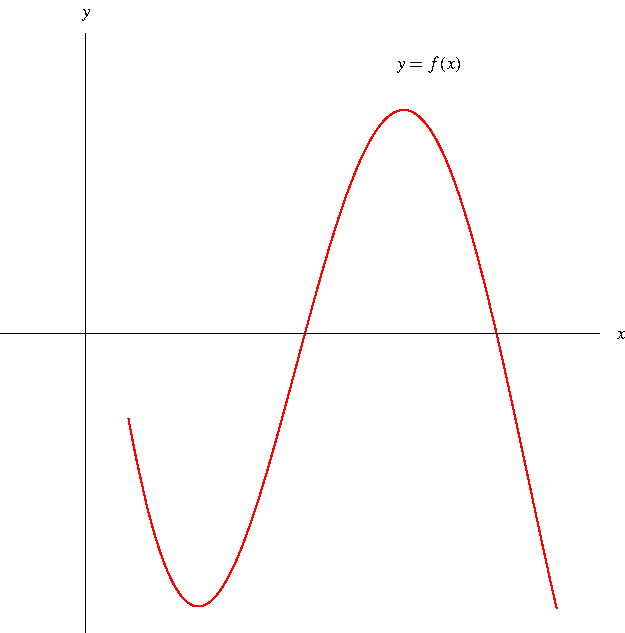
\includegraphics[height=4.2cm]{integration/pictures/05-02-net-area-function.pdf}%
%}%
%\only<handout:0| 11>{%
%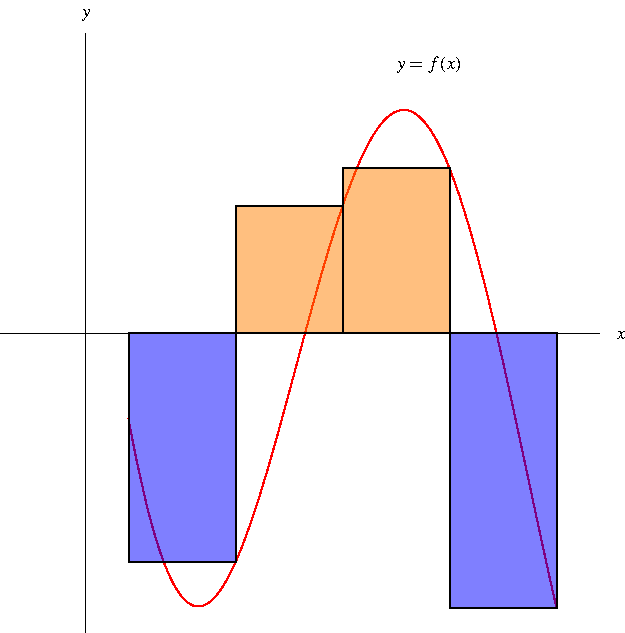
\includegraphics[height=4.2cm]{integration/pictures/05-02-net-areaa.pdf}%
%}%
%\only<handout:0| 12>{%
%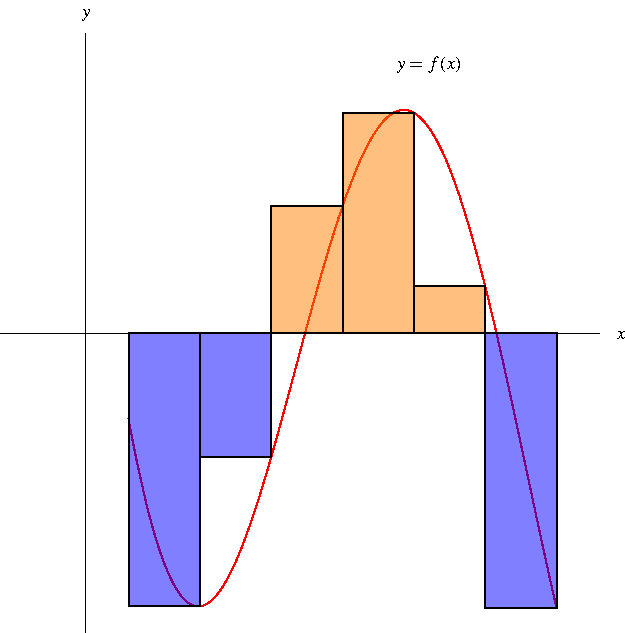
\includegraphics[height=4.2cm]{integration/pictures/05-02-net-areab.pdf}%
%}%
%\only<handout:0| 13>{%
%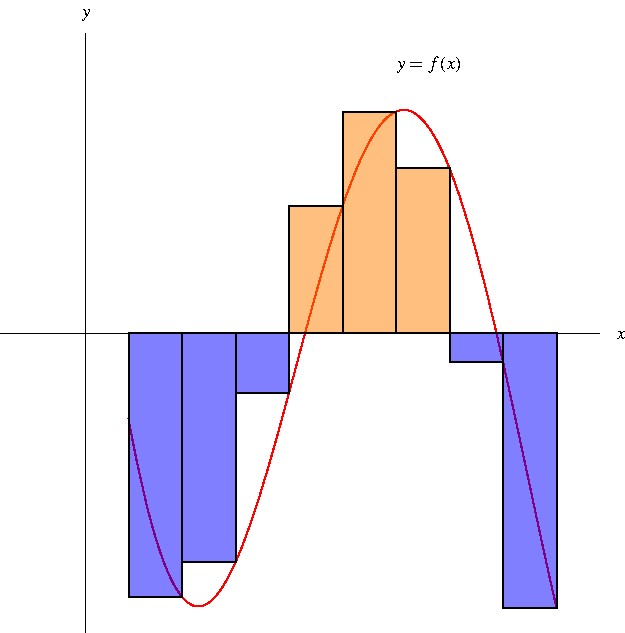
\includegraphics[height=4.2cm]{integration/pictures/05-02-net-areac.pdf}%
%}%
%\only<handout:0| 14>{%
%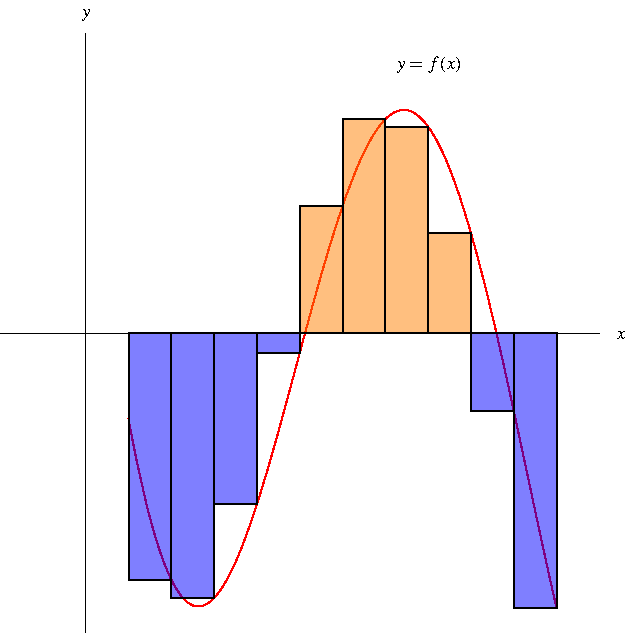
\includegraphics[height=4.2cm]{integration/pictures/05-02-net-aread.pdf}%
%}%
%\only<handout:0| 15>{%
%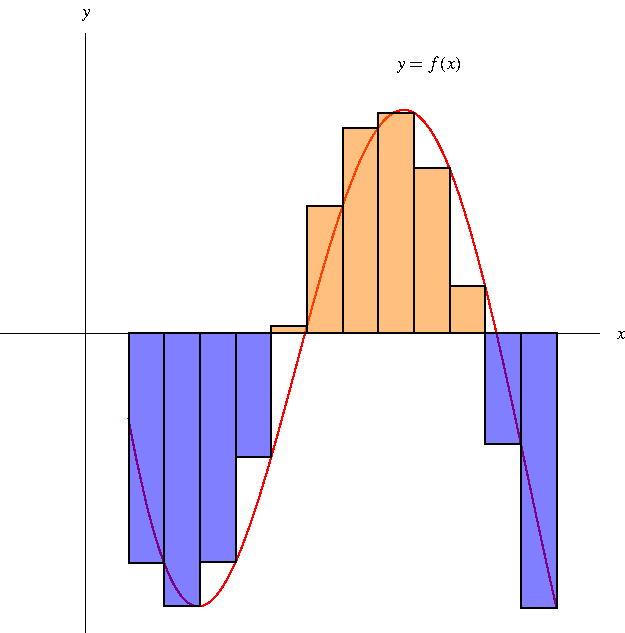
\includegraphics[height=4.2cm]{integration/pictures/05-02-net-areae.pdf}%
%}%
%\only<handout:0| 16>{%
%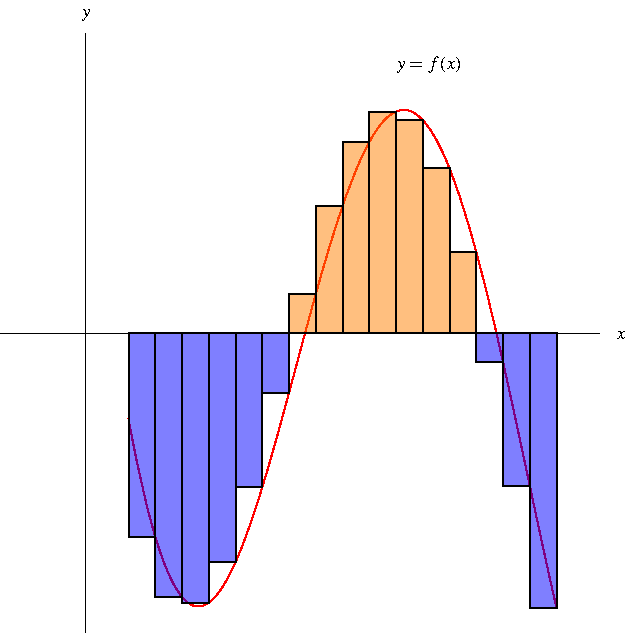
\includegraphics[height=4.2cm]{integration/pictures/05-02-net-areaf.pdf}%
%}%
%\only<handout:0| 17>{%
%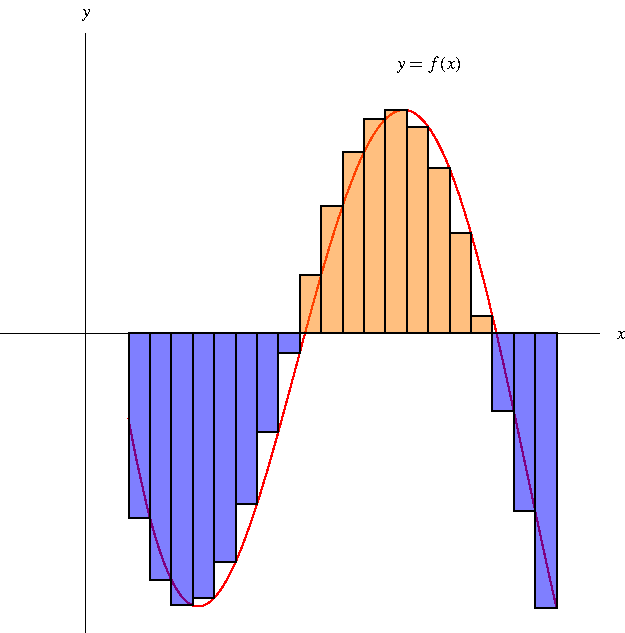
\includegraphics[height=4.2cm]{integration/pictures/05-02-net-areag.pdf}%
%}%
%\only<handout:0| 18>{%
%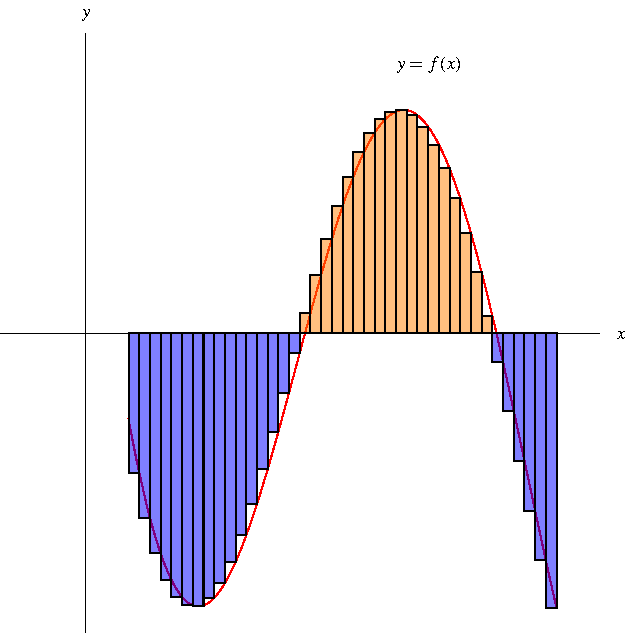
\includegraphics[height=4.2cm]{integration/pictures/05-02-net-areah.pdf}%
%}%
%\only<handout:1| 19->{%
%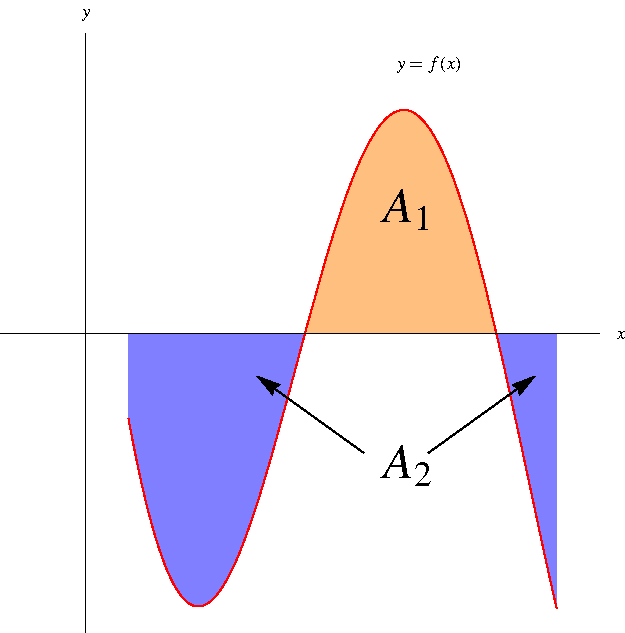
\includegraphics[height=4.2cm]{integration/pictures/05-02-net-area-limit.pdf}%
%}%
}%
\column{.6\textwidth}
\begin{itemize}
\item<10->  What if $f(x)$ is sometimes negative?
\uncover<handout:2|19->{
\item<19->  Then $\int_a^bf(x)\diff x = A_1 - A_2$.
\item<19->  $A_1$ is the area of the region above the $x$-axis and below the graph of $f$.
\item<19->  $A_2$ is the area of the region below the $x$-axis and above the graph of $f$.
}
\end{itemize}
\end{columns}
\end{frame}
% end module definite-integral-negative

\subsection{Evaluating Integrals}
% begin module definite-integral-ex2
\begin{frame}
\begin{example}
\begin{columns}
\column{0.15\textwidth}
\psset{xunit=0.2cm, yunit=0.2cm}
\begin{pspicture}(-0.5,-0.5)(3.1,9.1)
\fcBoundingBox{-1}{-7}{4}{9}
\pscustom*[linecolor=\fcColorNegativeAreaUnderGraph]{
%Function formula: x^{3}-6 x 
\psplot{0}{6 sqrt}{x -6 mul x 3 exp add }\psline(! 6 sqrt 2 1.5 exp 6 sqrt 6 mul sub)(! 6 sqrt  0)}
\pscustom*[linecolor=\fcColorAreaUnderGraph]{
%Function formula: x^{3}-6 x 
\psplot{6 sqrt}{3}{x -6 mul x 3 exp add }\psline(3, 9)(3,  0)}
\fcAxesStandardNoFrame{-1}{-7}{4}{9}
%Function formula: x^{3}-6 x 
\psplot[linecolor=\fcColorGraph, plotpoints=1000]{0}{3}{x -6 mul x 3 exp add }
\end{pspicture}
\column{0.85\textwidth}
Evaluate $\int_0^3 (x^3 - 6x)\diff x$. \uncover<2->{\alert<handout:0| 2-3,6>{ $\Delta x = \frac{b-a}{n} = \uncover<3->{\frac{3}{n}.}$}}

\abovedisplayskip=0pt
\belowdisplayskip=0pt
\abovedisplayshortskip=0pt
\belowdisplayshortskip=0pt
\begin{align*}
&\invisible{=}  \uncover<4->{%
\int_0^3 (x^3-6x)\diff x%
}%
\uncover<4->{%
 =  \lim_{n\to\infty} \sum_{i=1}^n f(\alert<handout:0| 7-8>{x_i})\alert<handout:0| 5-6>{\Delta x}%
}%
\uncover<5->{%
 = \lim_{n\to\infty} \sum_{i=1}^n f\left(\uncover<8->{\alert<handout:0| 8>{\frac{3i}{n}}}\right)\uncover<6->{\alert<handout:0| 6>{\frac{3}{n}}}%
}\\%
 & \uncover<9->{ = }  \uncover<9->{%
\lim_{n\to\infty} \frac{3}{n}\sum_{i=1}^n \left[ \left(\frac{3i}{n}\right)^3 - 6\left(\frac{3i}{n}\right)\right]%
}%
\uncover<10->{%
  =  \lim_{n\to\infty} \frac{3}{n}\sum_{i=1}^n \left[ \frac{27}{n^3}i^3 - \frac{18}{n}i\right]%
}\\%
 & \uncover<11->{ = }  \uncover<11->{%
\lim_{n\to\infty} \left[ \frac{81}{n^4}\alert<handout:0| 12-13>{\sum_{i=1}^n i^3} - \frac{54}{n^2} \alert<handout:0| 14-15>{\sum_{i=1}^n i}\right]%
}\\%
 & \uncover<12->{ = }  \uncover<12->{%
\lim_{n\to\infty} \left( \frac{81}{n^4}\uncover<13->{\alert<handout:0| 13>{\left[ \frac{n(n+1)}{2}\right]^2}} - \frac{54}{n^2} \uncover<15->{\alert<handout:0| 15>{\frac{n(n+1)}{2}}}\right)%
}\\%
 & \uncover<16->{ = }  \uncover<16->{%
\lim_{n\to\infty} \left[ \frac{81}{4}\left( 1 + \frac{1}{n}\right)^2 - 27 \left( 1 + \frac{1}{n}\right) \right]%
}%
\uncover<17->{%
 = \frac{81}{4} - 27 = -\frac{27}{4}
}%
\end{align*}
\end{columns}

\end{example}
\end{frame}
% end module definite-integral-ex2

\subsection{Properties of the Definite Integral}
% WARNING: This next module could use some pictures.

% begin module definite-integral-properties
\begin{frame}
\frametitle{Properties of the Definite Integral}
\begin{itemize}
\item  So far when we have calculated $\int_a^b f(x)\diff x$, we have assumed that $a < b$.
\item  The definition as a limit of Riemann sums will still work even if we don't assume this.
\item<2->  If we reverse $a$ and $b$, then $\Delta x$ changes from $\frac{b-a}{n}$ to $\frac{a-b}{n}$.
\end{itemize}
\[
\uncover<3->{%
\alert<handout:0| 3-4>{%
\int_b^a f(x)\diff x = %
}%
}%
\uncover<4->{%
\alert<handout:0| 3-4>{%
- \int_a^b f(x)\diff x %
}%
}%
\]
\begin{itemize}
\item<5-| alert@5-6>  If $a = b$, then $\Delta x = $ \uncover<6->{$0$.}
\end{itemize}
\[
\uncover<7->{%
\alert<handout:0| 7-8>{%
\int_a^a f(x) \diff x = %
}%
}%
\uncover<8->{%
\alert<handout:0| 7-8>{%
0 %
}%
}%
\]
\end{frame}

\begin{frame}
Properties of the Integral
\begin{enumerate}
\item<1-| alert@2>  $\int_a^b c\diff x = c(b-a)$, where $c$ is any constant.
\item<1-| alert@3>  $\int_a^b [f(x)+g(x)] \diff x = \int_a^b f(x)\diff x + \int_a^b g(x) \diff x$.
\item<1-| alert@4>  $\int_a^b cf(x) \diff x = c\int_a^b f(x)\diff x$, where $c$ is any constant.
\item<1-| alert@5>  $\int_a^b [f(x)-g(x)] \diff x = \int_a^b f(x)\diff x - \int_a^b g(x) \diff x$.
\end{enumerate}
\end{frame}
% end module definite-integral-properties

% begin module definite-integral-properties-ex6
\begin{frame}
\begin{example}[Example 6, p. 308]
Use the properties of integrals to evaluate
\begin{eqnarray*}
\alert<handout:0| 2-3>{\int_0^1 (4+3x^2)\diff x }%
& \uncover<2->{ = } &%
\uncover<2->{%
\alert<handout:0| 2-3>{\int_0^1 4\diff x + \int_0^1 \alert<handout:0| 4-5>{3}x^2\diff x \qquad \textrm{Property} \ \uncover<3->{2}}%
}\\%
& \uncover<4->{ = } &%
\uncover<4->{%
\alert<handout:0| 6-8>{\int_0^1 4\diff x} + \alert<handout:0| 4-5>{3}\int_0^1 x^2\diff x \qquad \alert<handout:0| 4-5>{\textrm{Property} \ \uncover<5->{3}}%
}\\%
& \uncover<6->{ = } &%
\uncover<6->{%
\alert<handout:0| 6-8>{\uncover<7->{4(1-0)}} + 3\alert<handout:0| 9-10>{\int_0^1 x^2\diff x} \qquad \alert<handout:0| 6-8>{\textrm{Property} \ \uncover<8->{1}}%
}\\%
& \uncover<9->{ = } &%
\uncover<9->{%
4 + 3\cdot \alert<handout:0| 9-10>{\uncover<10->{\frac{1}{3}}} \qquad \alert<handout:0| 10>{\uncover<10->{\textrm{Example 1, p. 289}}}%
}\\%
& \uncover<11->{ = } &%
\uncover<11->{%
5%
}%
\end{eqnarray*}
\end{example}
\end{frame}
% end module definite-integral-properties-ex6

% WARNING: This next module could use some pictures.
% begin module definite-integral-properties-split
\begin{frame}[t]
Properties of the Integral
\begin{enumerate}
\setcounter{enumi}{4}
\item  $\displaystyle %
\alertNoH{ 1}{\int_a^b f(x) \diff x} %
= %
\alertNoH{ 2}{\int_a^c f(x) \diff x} %
+ %
\alertNoH{ 3}{\int_c^b f(x) \diff x} %
$%
\end{enumerate}
\begin{center}
\psset{xunit=1.5cm, yunit=1.5cm}
\begin{pspicture}(-0.5,-0.5)(4.5,3.6)
\psframe*[linecolor=white](-0.5,-0.5)(4.5,3.6)
%Function formula: 1727/6250+4911/100 ((x)^{3})+110043/5000 (x)+3 ((x)^{5})-201/10 ((x)^{4})-52431/1000 ((x)^{2})
\uncover<1>{
\pscustom*[linecolor=\fcColorAreaUnderGraph]{
\psplot[linecolor=red, plotpoints=1000]{0.1}{2.5}{x 2 exp -52.431 mul x 4 exp -20.1 mul x 5 exp 3 mul x 22.0086 mul x 3 exp 49.11 mul 0.27632 add add add add add }
\psline(2.5, 0)(0.1,0)
}
}
\uncover<2>{
\pscustom*[linecolor=\fcColorAreaUnderGraph]{
\psplot[linecolor=red, plotpoints=1000]{0.1}{1.7}{x 2 exp -52.431 mul x 4 exp -20.1 mul x 5 exp 3 mul x 22.0086 mul x 3 exp 49.11 mul 0.27632 add add add add add }
\psline(1.7, 0)(0.1,0)
}
}
\uncover<3>{
\pscustom*[linecolor=\fcColorAreaUnderGraph]{
\psplot[linecolor=red, plotpoints=1000]{1.7}{2.5}{x 2 exp -52.431 mul x 4 exp -20.1 mul x 5 exp 3 mul x 22.0086 mul x 3 exp 49.11 mul 0.27632 add add add add add }
\psline(2.5, 0)(1.7,0)
}
}

\psline(0.1, 0.05)(0.1, -0.05)
\rput[t](0.1, -0.07){$a$}
\psline(1.7, 0.05)(1.7, -0.05)
\rput[t](1.7, -0.07){$c$}
\psline(2.5, 0.05)(2.5, -0.05)
\rput[t](2.5, -0.07){$b$}
\rput(1.5, 2.4 ){$y=f(x)$}
\psaxes[ticks=none, labels=none]{<->}(0,0)(-0.5,-0.5)(4,2.7)\tiny
\psplot[linecolor=red, plotpoints=1000]{0.1}{2.5}{x 2 exp -52.431 mul x 4 exp -20.1 mul x 5 exp 3 mul x 22.0086 mul x 3 exp 49.11 mul 0.27632 add add add add add }
\end{pspicture}
%\only<handout:0| -1>{%
%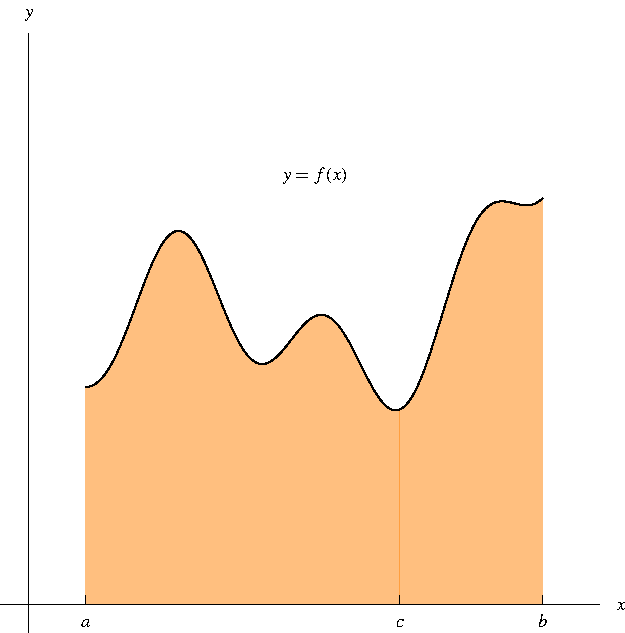
\includegraphics[height=5.6cm]{integration/pictures/05-02-splita.pdf}%
%}%
%\only<handout:0| 2>{%
%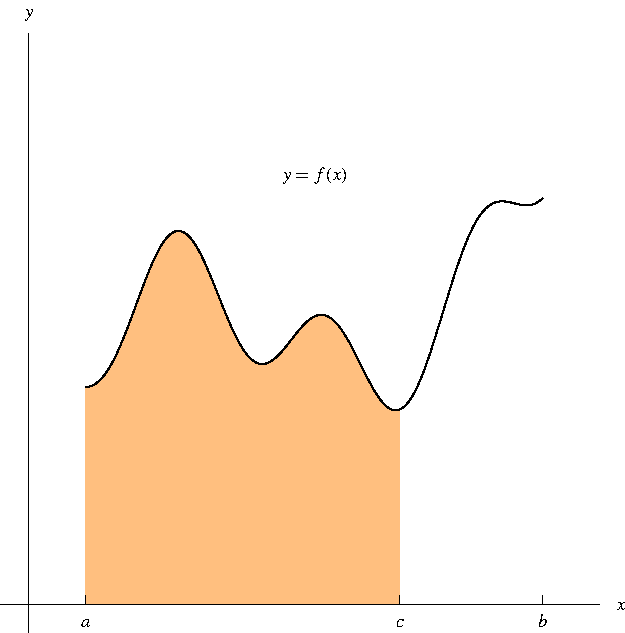
\includegraphics[height=5.6cm]{integration/pictures/05-02-splitb.pdf}%
%}%
%\only<handout:0| 3>{%
%\includegraphics[height=5.6cm]{integration/pictures/05-02-splitc.pdf}%
%}%
\end{center}
\end{frame}
% end module definite-integral-properties-split

% begin module definite-integral-properties-ex7
\begin{frame}
\begin{example} %[Example 7, p. 352]
If it is known that \alert<handout:0| 5-6>{$\int_0^{10}f(x)\diff x = 17$} and \alert<handout:0| 7-8>{$\int_0^8 f(x) \diff x = 12$}, then find $\int_8^{10}f(x) \diff x$.
\abovedisplayskip=0pt
\belowdisplayskip=0pt
\abovedisplayshortskip=0pt
\belowdisplayshortskip=0pt
\begin{align*}
\uncover<2->{%
\int_{\alert<handout:0| 2-3>{0}}^{\alert<handout:0| 2-3>{8}} f(x)\diff x + \int_{\alert<handout:0| 2-3>{8}}^{\alert<handout:0| 2-3>{10}}f(x)\diff x%
}%
& \uncover<3->{ = } %
\uncover<3->{%
\int_{\alert<handout:0| 3>{0}}^{\alert<handout:0| 3>{10}}f(x)\diff x%
}\\%
\uncover<4->{%
\int_{\alert<handout:0| 2-3>{8}}^{\alert<handout:0| 2-3>{10}}f(x)\diff x%
}%
& \uncover<4->{ = } %
\uncover<4->{%
\alert<handout:0| 5-6>{\int_{\alert<handout:0| 3>{0}}^{\alert<handout:0| 3>{10}}f(x)\diff x} - \alert<handout:0| 7-8>{\int_{\alert<handout:0| 2-3>{0}}^{\alert<handout:0| 2-3>{8}} f(x)\diff x}%
}\\%
& \uncover<5->{ = } %
\uncover<5->{%
\alert<handout:0| 5-6>{\uncover<6->{17}} - \alert<handout:0| 7-8>{\uncover<8->{12}}%
}\\%
& \uncover<9->{ = } %
\uncover<9->{%
5%
}%
\end{align*}
\end{example}
\end{frame}
% end module definite-integral-properties-ex7

% WARNING: This next module could use some pictures.
% begin module definite-integral-properties-comparison
\begin{frame}[t]
Comparison Properties of the Integral
\begin{enumerate}
\setcounter{enumi}{5}
\item  If $f(x)\geq 0$ for all $a\leq x \leq b$, then $\displaystyle \int_{a}^{b} f(x)\diff x \geq 0$.
\end{enumerate}
\end{frame}

\begin{frame}[t]
Comparison Properties of the Integral
\begin{enumerate}
\setcounter{enumi}{6}
\item  If $f(x)\leq g(x)$ for all $a\leq x \leq b$, then $\displaystyle \int_{a}^{b} f(x)\diff x \leq \int_{a}^{b} g(x)\diff x$.
\end{enumerate}
\begin{center}
\psset{xunit=0.9cm, yunit=0.9cm}
\begin{pspicture}(-0.5,-0.5)(6,4.5)
\psframe*[linecolor=white](-0.5,-0.5)(6,4.5)
\tiny
\rput[l](5.1, 2.6){$y=g(x)$}
\rput[l](5.1, 1.3){$y=f(x)$}
\uncover<2>{
\pscustom*[linecolor=cyan]{
\psplot[linecolor=red, plotpoints=1000]{0.2}{5}{x 2 exp -0.18 mul x 3 exp 0.025 mul x 0.368 mul 0.808 add add add }
\psline(5,0)(0.2,0)
}
}
\uncover<3->{
\pscustom*[linecolor=cyan]{
\psplot[linecolor=red, plotpoints=1000]{0.2}{5}{x -9.9495 mul x 3 exp -2.0625 mul x 4 exp 0.1875 mul x 2 exp 7.4925 mul 5.6936 add add add add }
\psline(5,0)(0.2,0)
}
}
%Function formula: 101/125+46/125 (x)+1/40 ((x)^{3})-9/50 ((x)^{2})
\psplot[linecolor=red, plotpoints=1000]{0.2}{5}{x 2 exp -0.18 mul x 3 exp 0.025 mul x 0.368 mul 0.808 add add add }
%Function formula: 7117/1250+2997/400 ((x)^{2})+3/16 ((x)^{4})-33/16 ((x)^{3})-19899/2000 (x)
\psaxes[ticks=none, labels=none]{<->}(0,0)(-0.5,-0.5)(6,4.5)
\psplot[linecolor=red, plotpoints=1000]{0.2}{5}{x -9.9495 mul x 3 exp -2.0625 mul x 4 exp 0.1875 mul x 2 exp 7.4925 mul 5.6936 add add add add }
\psline(0.2, -0.1)(0.2, 0.1)
\rput[t](0.2, -0.15){$a$}
\psline(5, -0.1)(5, 0.1)
\rput[t](5, -0.15){$b$}
\end{pspicture}
%\only<handout:0| -1>{%
%\includegraphics[height=4.2cm]{integration/pictures/05-02-comparisona.pdf}%
%}%
%\only<handout:0| 2>{%
%\includegraphics[height=4.2cm]{integration/pictures/05-02-comparisonb.pdf}%
%}%
%\only<handout:0| 3>{%
%\includegraphics[height=4.2cm]{integration/pictures/05-02-comparisonc.pdf}%
%}%
\[
\alertNoH{ 2}{\int_a^b f(x) \diff x}%
 \leq  %
\alertNoH{ 3}{\int_a^b g(x) \diff x}%
\]
\end{center}
\end{frame}

\begin{frame}[t]
Comparison Properties of the Integral
\begin{enumerate}
\setcounter{enumi}{7}
\item  If $m\leq f(x)\leq M$ for all $a\leq x \leq b$, then
\[
\alertNoH{ 2}{m(b-a)}%
 \leq  %
\alertNoH{ 3}{\int_a^b f(x) \diff x}%
 \leq  %
\alertNoH{ 4}{M(b-a)}%
\]
\end{enumerate}
\begin{center}
\psset{xunit=0.9cm, yunit=0.9cm}
\begin{pspicture}(-0.5,-0.5)(6,4.5)
\psframe*[linecolor=white](-0.5,-0.5)(6,4.5)
\tiny
\uncover<2>{
\pscustom*[linecolor=orange]{
\psplot[linecolor=\fcColorGraph, plotpoints=1000]{0.2}{5}{0.7}
\psline(5,0)(0.2,0)
}
}

\uncover<3>{
\pscustom*[linecolor=cyan!50]{
\psplot[linecolor=\fcColorGraph, plotpoints=1000]{0.2}{5}{x -9.9495 mul x 3 exp -2.0625 mul x 4 exp 0.1875 mul x 2 exp 7.4925 mul 5.6936 add add add add }
\psline(5,0)(0.2,0)
}
}
\uncover<4>{
\pscustom*[linecolor=cyan]{
\psplot[linecolor=red, plotpoints=1000]{0.2}{5}{4.3}
\psline(5,0)(0.2,0)
}
}
%Function formula: 7117/1250+2997/400 ((x)^{2})+3/16 ((x)^{4})-33/16 ((x)^{3})-19899/2000 (x)
\psaxes[ticks=none, labels=none]{<->}(0,0)(-0.5,-0.5)(6,4.5)
\psplot[linecolor=\fcColorGraph, plotpoints=1000]{0.2}{5}{x -9.9495 mul x 3 exp -2.0625 mul x 4 exp 0.1875 mul x 2 exp 7.4925 mul 5.6936 add add add add }
\psline[linecolor=\fcColorGraph](0.2, 0.7)(5,0.7)
\psline[linecolor=\fcColorGraph](0.2, 4.3)(5, 4.3)


\rput[r](4.9, 2.6){\alertNoH{3}{$y=f(x)$}}
\psline[linestyle=dotted, arrows=<->](5.05, 0)(5.05, 0.7)
\rput[l](5.15,0.35){\alertNoH{2}{$m$}}
\psline[linestyle=dotted, arrows=<->](5.5, 0)(5.5, 4.3)
\rput[l](5.6,2.15){\alertNoH{4}{$M$}}

\psline(0.2, -0.1)(0.2, 0.1)
\rput[t](0.2, -0.15){\alertNoH{2,4}{$a$}}
\psline(5, -0.1)(5, 0.1)
\rput[t](5, -0.15){\alertNoH{2,4}{$b$}}
\end{pspicture}
%\only<handout:0| -1>{%
%\includegraphics[height=5.6cm]{integration/pictures/05-02-boundinga.pdf}%
%}%
%\only<handout:0| 2>{%
%\includegraphics[height=5.6cm]{integration/pictures/05-02-boundingb.pdf}%
%}%
%\only<handout:0| 3>{%
%\includegraphics[height=5.6cm]{integration/pictures/05-02-boundingc.pdf}%
%}%
%\only<handout:0| 4>{%
%\includegraphics[height=5.6cm]{integration/pictures/05-02-boundingd.pdf}%
%}%
\end{center}
\end{frame}
% end module definite-integral-properties-comparison

}% end lecture


\lect{Week 2}{Definite Integrals and FTC2}{2}{% begin lecture
\section{Evaluating Definite Integrals}
\subsection{The Evaluation Theorem (FTC part 2)}
% begin module FTC-part2
\begin{frame}
\uncover<3->{
\begin{theorem}
Let $f$ be a continuous function on $[a,b]$. Then $f$ is integrable over $[a,b]$.
\end{theorem}
}
\uncover<2->{
\uncover<3->{In other words,} \alert<2>{$\displaystyle\int_a^{b}f(x)dx $ is defined for any continuous (over $[a,b]$) function $f$}.
}

\begin{theorem}[The Evaluation Theorem (FTC part 2)]
If \alert<2>{$f$ is continuous on $[a, b]$}, then
\[
\alert<2>{\int_a^b f(x) \diff x} = F(b) - F(a),
\]
where $F$ is any antiderivative of $f$.
\end{theorem}

\end{frame}
% end module FTC-part2

% begin module FTC-part2-ex5
\begin{frame}
\begin{example}%[Example 5, p. 318]
\begin{columns}
\column{.1\textwidth}
\psset{xunit=0.4cm, yunit=0.4cm}
\begin{pspicture}(-2.500000, -5)(1.500000,5)
\psframe*[linecolor=white](-2.500000,-9)(1.500000,5)
\tiny
\pscustom*[linecolor=cyan]{ %Function formula: x^{3}
\psplot[linecolor=\fcColorGraph, plotpoints=1000]{0}{1}{x 3 exp }\psline(1.000000, 0)(0.000000, 0)}
%Function formula: x^{3}
\psplot[linecolor=\fcColorGraph, plotpoints=1000]{0}{1}{x 3 exp }
\pscustom*[linecolor=orange]{ %Function formula: x^{3}
\psplot[linecolor=\fcColorGraph, plotpoints=1000]{-2}{0}{x 3 exp }\psline(0.000000, 0)(-2.000000, 0)}
\psplot[linecolor=\fcColorGraph, plotpoints=1000]{-2}{0}{x 3 exp }
\psaxes[ticks=none, labels=none]{<->}(0,0)(-2.2,-8)(1.2,1)
\fcLabels{1.2}{1}
\end{pspicture}
\column{.9\textwidth}
Evaluate the integral $\displaystyle\int_{-2}^1 x^3 \ \diff x$.
\begin{itemize}
\item<2->  $x^3$ is continuous on $[-2, 1]$ (in fact, it's continuous everywhere).
\item<3->  An antiderivative is \alertNoH{ 3-4}{$F(x) = $ $\fcAnswer{4}{\frac{1}{4}x^4.}$}
\end{itemize}
\[
\uncover<5->{%
\int_{\alertNoH{ 5}{-2}}^{\alertNoH{ 5}{1}} x^3 \ \diff x = F(\alertNoH{ 5}{1}) - F(\alertNoH{ 5}{-2}) %
}%
\uncover<6->{%
 = \frac{1}{4}(1)^4 - \frac{1}{4}(-2)^4 %
}%
\uncover<7->{%
 = \frac{1}{4} - \frac{16}{4} = -\frac{15}{4} %
}%
\]
\end{columns}
\end{example}
\end{frame}
% end module FTC-part2-ex5

% begin module indefinite-integral
\begin{frame}
We often use the notation
\[
\left. F(x)\right]_a^b = F(b)-F(a)
\]
or 
\[
\left[ F(x)\right]_a^b = F(b)-F(a)
\]
Therefore we can write
\[
\int_a^b f(x) \diff x = \left. F(x)\right]_a^b
\]
or
\[
\int_a^b f(x) \diff x = \left[ F(x)\right]_a^b
\]
\end{frame}
% end module indefinite-integral

% begin module FTC-part2-ex6
\begin{frame}
\begin{example}%[Example 6, p. 319]
\begin{columns}
\column{0.1\textwidth}
\psset{xunit=1cm, yunit=1cm}
\begin{pspicture}(-1.000000, -5)(1.500000,5) 
\psframe*[linecolor=white](-1.000000,-5)(1.500000,5) 
\tiny 
\pscustom*[linecolor=cyan]{ %Function formula: x^{2} 
\psplot[linecolor=\psColorGraph, plotpoints=1000]{0}{1}{x 2 exp }\psline(1.000000, 0)(0.000000, 0)}
\psplot[linecolor=\psColorGraph, plotpoints=1000]{0}{1}{x 2 exp }
\psaxes[ticks=none, labels=none]{<->}(0,0)(-0.500000,-0.5)(1.1,1.1)
\psLabels{1.1}{1.1}
\end{pspicture} 
\column{0.9\textwidth}
Find the area under the parabola $y = x^2$ from $0$ to $1$.
\begin{itemize}
\item<2->  $x^2$ is continuous on $[0, 1]$ (in fact, it's continuous everywhere).
\item<3-| alert@3-4>  An antiderivative is \uncover<4->{$\frac{1}{3}x^3$.}
\end{itemize}
\[
\uncover<5->{%
\int_{\alert<handout:0| 5>{0}}^{\alert<handout:0| 5>{1}} x^2 \ \diff x = \left[ \frac{1}{3}x^3\right]_{\alert<handout:0| 5>{0}}^{\alert<handout:0| 5>{1}} %
}%
\uncover<6->{%
 = \frac{1}{3}(1)^3 - \frac{1}{3}(0)^3 %
}%
\uncover<7->{%
 = \frac{1}{3}%
}%
\]
\end{columns}
\end{example}
\end{frame}
% end module FTC-part2-ex6

% begin module FTC-part2-ex7
\begin{frame}
\begin{example} %[Example 2, p. 357]
\begin{columns}
\column{0.2\textwidth}
\psset{xunit=0.4cm, yunit=0.4cm}
\begin{pspicture}(-1.000000, -5)(1.500000,5) 
\psframe*[linecolor=white](-1.000000,-5)(7,5) 
\tiny 
\pscustom*[linecolor=cyan]{ %Function formula: \cos{}x 
\psplot[linecolor=\psColorGraph, plotpoints=1000]{0}{1}{x 57.29578 mul cos }\psline(1.000000, 0)(0.000000, 0)}
%Function formula: \cos{}x 
\psplot[linecolor=\psColorGraph, plotpoints=1000]{0}{6}{x 57.29578 mul cos }
\psaxesStandard{-0.6}{-0.6}{6}{1.1}
\end{pspicture} 
\column{0.8\textwidth}
Find the area under the cosine curve from $0$ to $b$, where $0 \leq b \leq \pi /2$.
\begin{itemize}
\item<2->  $\cos x$ is continuous on $[0, \pi /2]$ (in fact, it's continuous everywhere).
\item<3-| alert@3-4>  An antiderivative is \uncover<4->{$\sin x$.}
\end{itemize}
\[
\uncover<5->{%
\int_{\alert<handout:0| 5>{0}}^{\alert<handout:0| 5>{b}} \cos x \ \diff x = \left[ \sin x \right]_{\alert<handout:0| 5>{0}}^{\alert<handout:0| 5>{b}} %
}%
\uncover<6->{%
 = \sin (b) - \sin (0)%
}%
\uncover<7->{%
 = \sin b%
}%
\]
\end{columns}
\end{example}
\end{frame}
% end module FTC-part2-ex7

\subsection{Indefinite Integrals}
% begin module indefinite-integral-intro
\begin{frame}\frametitle{Indefinite Integrals}
\begin{itemize}
\item  The Evaluation Theorem establishes a connection between antiderivatives and definite integrals.
\item  It says that $\int_a^b f(x)\diff x$ equals $F(b) - F(a)$, where $F$ is an antiderivative of $f$.
\item  We need convenient notation for writing antiderivatives: The indefinite integral
\end{itemize}
\begin{definition}[Indefinite Integral]
The indefinite integral of $f$ is another way of writing the general antiderivative of $f$, and is written $\int f(x) \diff x$.  In other words,
\abovedisplayskip=0pt
\belowdisplayskip=0pt
\[
\int f(x) \diff x = F(x)+C, \quad \text{means} \quad F'(x) = f(x). 
\]
($ C $ an arbitrary constant)

\end{definition}
\end{frame}

\begin{frame}
\begin{example}
\abovedisplayskip=0pt
\belowdisplayskip=0pt
\[
\int x^4 \diff x = \uncover<2->{\frac{x^5}{5}} \uncover<3->{\alert<handout:0| 3>{+ C}}
\]
\uncover<4->{because}
\abovedisplayskip=0pt
\belowdisplayskip=0pt
\[
\uncover<4->{\frac{\diff}{\diff x}\left( \frac{x^5}{5} + C\right) = x^4.}
\]
\end{example}
\begin{itemize}
\item<5->  The indefinite integral represents a whole family of functions.
\item<6->  Example: %1b, p. 318:  
the general antiderivative of $\frac{1}{x}$ is
\abovedisplayskip=0pt
\belowdisplayskip=0pt
\[
\uncover<6->{%
F(x) = \left\{ \begin{array}{ccc}
\ln |x| + C_1 & \text{ if } & x > 0\\
\ln |x| + C_2 & \text{ if } & x < 0
\end{array}\right.
}%
\]
\item<7->  We adopt the convention that the constant participating in an indefinite integral is only valid on one interval.
\item<8->  $\int \frac{1}{x} \diff x = \ln |x| + C$, and this is valid either on $(-\infty , 0)$ or $(0, \infty)$.
\end{itemize}
\end{frame}
% end module indefinite-integral-intro

% integral table
\begin{frame}\frametitle{Indefinite Integrals}

\tiny
\begin{columns}[t,onlytextwidth]
\column{.5\textwidth}
\begin{equation}
\int af(x)\dx = a\int f(x)\dx +C
\end{equation}

\begin{equation}
\int f(x)\pm g(x) \dx = \int f(x)\dx \pm \int g(x)\dx
\end{equation}

\begin{equation}
\int k\dx = kx+C
\end{equation}

\begin{equation}
\int x^n \dx = \frac{x^{n+1}}{n+1}+C, \hspace{1ex} n\neq-1
\end{equation}

\begin{equation}
\int \frac{1}{x}\dx = \ln |x|+C
\end{equation}

%\begin{equation}
%\int u \hspace{2pt} \dd{v} = uv - \int v du
%\end{equation}



\begin{equation}
\int e^x \dx = e^x +C
\end{equation}

\begin{equation}
\int a^x \dx = \frac{1}{\ln a} a^x+C
\end{equation}

%\begin{equation}
%\int \ln x \dx = x \ln x - x
%\end{equation}


\begin{equation}
\int \sin x \dx = -\cos x +C
\end{equation}

\column{.5\textwidth}
\begin{equation}
\int \cos x \dx = \sin x +C
\end{equation}


%\begin{equation}
%\int \tan x \dx = \ln |\sec x| +C 
%\end{equation}

%\begin{equation}
%\int \sec x \dx = \ln |\sec x + \tan x| +C
%\end{equation}


\begin{equation}
\int \sec^2 x \dx = \tan x +C
\end{equation}

\begin{equation}
\int \sec x \tan x \dx = \sec x +C
\end{equation}

\begin{equation}
\int \csc^2 x \dx = -\cot x +C
\end{equation}

\begin{equation}
\int \csc x \cot x \dx = -\csc x +C
\end{equation}


\begin{equation}
\int \frac{1}{1+x^2}\dx = \tan^{-1}x +C
\end{equation}

\begin{equation}
\int \frac{1}{\sqrt{1-x^2}} \dx = \sin^{-1}x +C
\end{equation}

\begin{equation}
\int \sinh(x) \dx = \cosh(x) +C
\end{equation}

\begin{equation}
\int \cosh(x) \dx = \sinh(x) +C
\end{equation}

%\begin{equation}
%\int \frac{a}{a^2+x^2}\dx = \tan^{-1}\frac{x}{a} +C
%\end{equation}


%\begin{equation}
%\int \frac{a}{a^2-x^2}\dx = %\frac{1}{2}\ln\left|\frac{x+a}{x-a}\right|+C
%\end{equation}

%\begin{equation}
%\int \frac{1}{\sqrt{a^2-x^2}} \dx = \sin^{-1} \frac{x}{a}+C
%\end{equation}

%\begin{equation}
%\int \frac{a}{x \sqrt{x^2-a^2}} \dx = \sec^{-1} \frac{x}{a}
%\end{equation}

%\begin{align}
%\int \frac{1}{\sqrt{x^2-a^2}} \dx &= \cosh^{-1} \frac{x}{a} \\&= %\nonumber \ln (x+\sqrt{x^2-a^2})
%\end{align}

%\begin{align}
%\int \frac{1}{\sqrt{x^2+a^2}} \dx &= \sinh^{-1} \frac{x}{a} %\\&=\nonumber \ln (x+\sqrt{x^2+a^2})
%\end{align}

\end{columns}
\end{frame}
% end module integral table

% begin module indefinite-integral-ex1
\begin{frame}
\begin{example} %[Example 3, p. 359]
Find the general indefinite integral.
\abovedisplayskip=0pt
\belowdisplayskip=0pt
\abovedisplayshortskip=0pt
\belowdisplayshortskip=0pt
\begin{align*}
\int (10x^4 - 2\sec^2 x )\diff x %
& \uncover<2->{=}  \uncover<2->{10\alert<handout:0| 3-4>{\int x^4 \diff x} - 2 \alert<handout:0| 5-6>{\int \sec^2 x \diff x}}\\
& \uncover<3->{=}  \uncover<3->{10 \uncover<4->{\alert<handout:0| 4>{\frac{x^5}{5}}} - 2 \uncover<6->{\alert<handout:0| 6>{\tan x}}} \uncover<7->{\alert<handout:0| 7>{+C}}\\
& \uncover<8->{=}  \uncover<8->{2x^5 - 2 \tan x + C}
\end{align*}
\end{example}
\end{frame}
% end module indefinite-integral-ex1

% begin module indefinite-integral-ex2
\begin{frame}
\begin{example}%[Example 2, p. 325]
Find the general indefinite integral.
\abovedisplayskip=0pt
\belowdisplayskip=0pt
\abovedisplayshortskip=0pt
\belowdisplayshortskip=0pt
\begin{align*}
\int \frac{\cos \theta}{\sin^2 \theta} \diff \theta %
& \uncover<2->{=}  \uncover<2->{\int \left( \alert<handout:0| 3-4>{\frac{1}{\sin \theta}}\right)\left(\alert<handout:0| 5-6>{\frac{\cos \theta}{\sin \theta}}\right)\diff \theta}\\
& \uncover<3->{=}  \uncover<3->{\alert<handout:0| 7-8>{\int \uncover<4->{\alert<handout:0| 4>{\csc \theta}} \uncover<6->{\alert<handout:0| 6>{\cot \theta}}\diff \theta}}\\
& \uncover<7->{=}  \uncover<8->{\alert<handout:0| 8>{-\csc \theta}} \uncover<9->{\alert<handout:0| 9>{+ C}}
\end{align*}
\end{example}
\end{frame}
% end module indefinite-integral-ex2

% begin module indefinite-integral-ex3
\begin{frame}
\begin{example}[Example 3, p. 326]
Evaluate.
\belowdisplayskip=0pt
\begin{eqnarray*}
\int_0^3 (x^3 - 6x)\diff x %
& \uncover<2->{=} & \uncover<2->{\left[ \int (x^3 - 6x)\diff x  \right]_0^3}\\%
& \uncover<3->{=} & \uncover<3->{\left[ \alert<handout:0| 4-5>{\int x^3 \diff x} - 6\alert<handout:0| 6-7>{\int x \diff x}  \right]_0^3}\\%
& \uncover<4->{=} & \uncover<4->{\left[ \alert<handout:0| 4-5>{\uncover<5->{\frac{x^4}{4}}} - 6\alert<handout:0| 6-7>{\uncover<7->{\frac{x^2}{2}}}  \right]_0^3}\\%
& \uncover<8->{=} & \uncover<8->{ \left( \frac{1}{4} \cdot 3^4 - 3\cdot 3^2 \right) - \left( \frac{1}{4}\cdot 0^4 - 3\cdot 0^2  \right) }\\%
& \uncover<9->{=} & \uncover<9->{ \frac{81}{4} - 27 - 0 + 0 = -\frac{27}{4}}
\end{eqnarray*}
\uncover<10->{Compare this with Example 2, p. 303.}
\end{example}
\end{frame}
% end module indefinite-integral-ex3

% begin module indefinite-integral-ex5
\begin{frame}
\begin{example} %[Example 6, p. 360]
\abovedisplayskip=0pt
\belowdisplayskip=0pt
\abovedisplayshortskip=0pt
\belowdisplayshortskip=0pt
\begin{align*}
\text{Evaluate: }& \invisible{ = } \int_1^9 \frac{2t^2 + t^2 \sqrt{t} - 1}{t^2} \diff t \\%
& \uncover<2->{=}  \uncover<2->{ \int_1^9 (2 + t^{1/2} - t^{-2})\diff t  }%
 \uncover<3->{=}  \uncover<3->{ \left[ \int (2 + t^{1/2} - t^{-2})\diff t \right]_1^9 }\\%
& \uncover<4->{=}  \uncover<4->{ \left[ \alert<handout:0| 5-6>{\int 2 \diff t} + \alert<handout:0| 7-8>{\int t^{1/2} \diff t} - \alert<handout:0| 9-10>{\int t^{-2} \diff t} \right]_1^9 }\\%
& \uncover<5->{=}  \uncover<5->{ \left[ \alert<handout:0| 5-6>{\uncover<6->{2t}} + \alert<handout:0| 7-8>{\uncover<8->{\frac{t^{3/2}}{3/2}}} - \alert<handout:0| 9-10>{\uncover<10->{\frac{t^{-1}}{-1}}} \right]_1^9 }%
 \uncover<11->{=}  \uncover<11->{ \left[ 2t + \frac{2}{3}t^{3/2} + \frac{1}{t}\right]_1^9}\\%
& \uncover<12->{=}  \uncover<12->{ \left( 2\cdot 9 + \frac{2}{3}\cdot 9^{3/2} + \frac{1}{9}  \right) - \left( 2\cdot 1 + \frac{2}{3}\cdot 1^{3/2} + \frac{1}{1}   \right)}\\%
& \uncover<13->{=}  \uncover<13->{ 18 + 18 + \frac{1}{9} - 2 - \frac{2}{3} - 1 }%
 \uncover<14->{=}  \uncover<14->{ \frac{292}{9}.}
\end{align*}
\end{example}
\end{frame}
% end module indefinite-integral-ex5

\section{The Fundamental Theorem of Calculus}
% begin module FTC-intro
\begin{frame}
\frametitle{(5.3) The Fundamental Theorem of Calculus}
\begin{itemize}
\item  The Fundamental Theorem of Calculus establishes a connection between differential calculus and integral calculus.
\item  It allows us to compute integrals very easily, without finding limits of Riemann sums.
\item  It has two different parts.
\item  Part 1 says, roughly, that ``differentiation undoes integration.''
\item  Part 2 says, roughly, that ``integration undoes differentiation.''
\item<2->  Part 1 deals with functions of the form
\[
\uncover<2->{%
g(x) = \int_a^x  f(t) \diff t%
}%
\]
\uncover<2->{where $f$ is a continuous function on $[a,b]$ and $x$ varies between $a$ and $b$.}
\end{itemize}
\end{frame}
% end module FTC-intro

% WARNING: This section could use more pictures.
% It would be nice to have animated pictures of the area-so-far function. Todor: Greg, what do you mean?
% begin module functions-defined-as-integrals
\begin{frame}
\[
g(x) = \int_a^{\alert<handout:0| 2>{x}}  f(t) \diff t%
\]
\begin{itemize}
\item<2->  $g$ depends only on \alert<handout:0| 2>{$x$}.
\item<3->  If $x$ is a fixed number, then $\int_a^x f(t)\diff t$ is a fixed number.
\item<4->  If we let $x$ vary, then $\int_a^x f(t)\diff t$ varies.
\item<5->  If $f$ is positive, then $g$ can be interpreted as the area under $f$ from $a$ to $x$.
\end{itemize}
\end{frame}
% end module functions-defined-as-integrals

% begin module FTC-part1-demo
\begin{frame}
\begin{example}[FTC Part 1]
\abovedisplayskip=0pt
\belowdisplayskip=0pt
\abovedisplayshortskip=0pt
\belowdisplayshortskip=0pt
\begin{align*}
\text{If } g(x) & = \int_1^x (\alert<handout:0| 2-3>{e^t} + \alert<handout:0| 4-5>{2t} )\diff t, \text{ find } g'(x).\\
\uncover<2->{g(x)} & \uncover<2->{= \left[ \alert<handout:0| 2-3>{\uncover<3->{e^t}} + \alert<handout:0| 4-5>{\uncover<5->{t^2}} \right]_1^x}\\
 & \uncover<6->{ = ( e^x + x^2) - (e^1 + 1^2)}\\
 & \uncover<7->{ = e^x + x^2 - e - 1.}\\
& \\
\uncover<8->{g'(x)} & \uncover<8->{ = \frac{\diff}{\diff x} ( \alert<handout:0| 9-10>{e^x} + \alert<handout:0| 11-12>{x^2} - \alert<handout:0| 13-14>{e} - \alert<handout:0| 15-16>{1} )}\\
 & \uncover<9->{ =  \alert<handout:0| 9-10>{\uncover<10->{e^x}} + \alert<handout:0| 11-12>{\uncover<12->{2x}} - \alert<handout:0| 13-14>{\uncover<14->{0}} - \alert<handout:0| 15-16>{\uncover<16->{0}} }\\
 & \uncover<17->{ = e^x + 2x.}
\end{align*}
\end{example}
\end{frame}
% end module FTC-part1-demo

% begin module FTC-part1
\begin{frame}
\begin{theorem}[The Fundamental Theorem of Calculus, Part 1]
If $f$ is continuous on $[a,b]$, then the function $g$ defined by
\[
g(x) = \int_a^x f(t)\diff t
\]
is continuous on $[a,b]$ and differentiable on $(a, b)$, and $g'(x) = f(x)$.
\end{theorem}
\end{frame}
% end module FTC-part1

% begin module FTC-part1-ex2
\begin{frame}
\begin{example}[Example 3, p. 370]
Find the derivative of $g(x) = \int_0^x \alert<handout:0| 4>{\sqrt{1+t^2}}\diff t$.
\begin{itemize}
\item<2->  $f(t) = \sqrt{1+t^2}$ is continuous.
\item<3->  By the FTC, Part 1,
\end{itemize}
\[
\uncover<3->{%
\alert<handout:0| 3-4>{g'(x) = \uncover<4->{\sqrt{1+x^2}}}%
}%
\]
\end{example}
\end{frame}
% end module FTC-part1-ex2

% begin module FTC-part1-exs
\begin{frame}
\begin{example}[FTC, Part 1]
For each formula $g(x)$, find the derivative $g'(x)$.
\[
\begin{array}{c|c}
g(x) & g'(x) \\
\hline
\alertNoH{ 2-3}{\displaystyle \int_0^x \sin(t^2+1)\cos(t^3+2)\diff t} & %
\alertNoH{ 2-3}{\uncover<3->{\displaystyle \sin(x^2+1)\cos(x^3+2)}} \\%
 & \\
\alertNoH{ 4-5}{\displaystyle \int_{35}^x \frac{1+r^2+4r^3}{1-r^4}\diff r} & %
\alertNoH{ 4-5}{\uncover<5->{\displaystyle \frac{1+x^2+4x^3}{1-x^4}}} \\%
 & \\
\alertNoH{ 6-7}{\displaystyle \int_{-1}^x \frac{\cos 2\theta + 1}{1+\sin^2 \theta}\diff \theta} & %
\alertNoH{ 6-7}{\uncover<7->{\displaystyle \frac{\cos 2x + 1}{1+\sin^2 x}}}%
\end{array}
\]
\end{example}
\end{frame}
% end module FTC-part1-exs

% begin module FTC-part1-ex4
\begin{frame}
\chainruley{\int_0^{x^4}\sec t \diff t}{x^4}{\int_0^u \sec t \diff t}{\sec UU}{4x^3}{4x^3\sec(UU)}{FTC Part 1, Example 5, p. 370}
\end{frame}
% end module FTC-part1-ex4

% begin module FTC-both
\begin{frame}
\begin{theorem}[The Fundamental Theorem of Calculus]
Suppose $f$ is continuous on $[a, b]$.  Then 
\begin{enumerate}
\item  If $g(x) = \displaystyle \int_a^x f(t) \diff t$, then $g'(x) = f(x)$.  
\item  $\displaystyle \int_a^b f(x) \diff x = F(b) - F(a),$ where $F$ is any antiderivative of $f$.
\end{enumerate}
\end{theorem}
We already studied part 2 of the FTC as the Evaluation Theorem.
\end{frame}
% end module FTC-both

%module FTC part1 solving problems.
\begin{frame}
\begin{theorem}
Let $A,B$-numbers, $a(x), b(x)$ -differentiable functions with $A<a(x)<B$, $A<b(x)<B$. Let $f$ - continuous on $[A,B]$  and $\displaystyle G(x)=\int_{a(x)}^{b(x)} f(t)dt$. Then  $ \alertNoH{11}{G'(x)=f(b(x))b'(x)-f(a(x))a'(x)}$.
\end{theorem}
\begin{proof}
\uncover<2->{\alertNoH{6}{Let $c\in (A, B)$}.} \uncover<3->{Set $\alertNoH{7}{\displaystyle h(u)=\int_{c}^{u}f(t)dt}$.} \uncover<4->{FTC part 1 states that $h'(u)=f(u)$.}

$\begin{array}{rcl}
\uncover<5->{\displaystyle G(x)&=&\displaystyle\int_{a(x)}^{b(x)} f(t)dt}\uncover<6->{= \int_{\alertNoH{6}{c}}^{b(x)} f(t)dt+ \int_{\alertNoH{7}{a(x)}}^{\alertNoH{6}{\alertNoH{7}{c}}} f(t)dt} \\
\uncover<7->{&=&\displaystyle \int_c^{b(x)} f(t)dt\alertNoH{7}{-}\int_{\alertNoH{7}{c}}^{\alertNoH{7}{a(x)}}f(t)dt}\uncover<8->{=\alertNoH{8}{h(b(x))-h(a(x)) } \quad.}
\end{array}$

\uncover<9->{Then} \uncover<10->{using the chain rule we get}

$ \uncover<9->{\displaystyle\alertNoH{11}{  G'(x)}= \left(h(b(x))-h(a(x)) \right)'} \uncover<10->{= h'(b(x)) b'(x)-h'(a(x))a'(x)}\uncover<11->{=\alertNoH{11}{f(b(x))b'(x)-f(a(x))a'(x)},}
$\uncover<11->{ as desired.}
\end{proof}
\end{frame}

\begin{frame}
Problems similar to the following often appear on Calculus I exams.
\begin{example}
Let $\displaystyle G(x)=\int_{\sqrt{x}}^{x^2}\ln t dt$, $x> 0$. Find $G'(x)$.

\[
\uncover<2->{G'(x)=(\ln x^2) (x^2)'-(\ln \sqrt{x}) (\sqrt{x})'}\uncover<3->{= \left(4x- \frac14 x^{-\frac12}\right)\ln x.}
\]

\end{example}
\end{frame}

%end module FTC part1 solving problems.

\subsection{Proof of FTC, part 1}
% begin module FTC1-proof
\begin{frame}
\begin{theorem}[The Fundamental Theorem of Calculus part 1]
Let \alertNoH{2}{$f$ be a function continuous on $[a, b]$} and let $G(x) = \displaystyle \int_a^x f(t) \diff t$ for all $x\in [a,b]$. Then $G$ is differentiable and $G'(x) = f(x)$.
\end{theorem}
\begin{proof}[Proof]
\begin{columns}
\column{0.27\textwidth}
\psset{xunit=0.9cm, yunit=0.9cm}

\begin{pspicture}(-0.6,-0.6)(3.3,3.3)
\psframe*[linecolor=white](-0.6,-0.6)(3.3,3.3)
\tiny
%\fcLabels{3}{2.5}

\pscustom*[linecolor=cyan]{
\psplot[linecolor=\fcColorGraph, plotpoints=1000]{0.5}{2}{1 -0.5 x add 3 exp 0.333333 mul add -0.5 x add 2 exp -0.5 mul add }
\psline(2,0)(0.5,0)
}
\uncover<20,21>{
\pscustom*[linecolor=red]{
\psplot[linecolor=\fcColorGraph, plotpoints=1000]{0.5}{2}{1 -0.5 x add 3 exp 0.333333 mul add -0.5 x add 2 exp -0.5 mul add }
\psline(2,0)(0.5,0)
}
}

\uncover<11->{
\pscustom*[linecolor=blue]{
\psplot[linecolor=\fcColorGraph, plotpoints=1000]{2}{2.15}{1 -0.5 x add 3 exp 0.333333 mul add -0.5 x add 2 exp -0.5 mul add }
\psline(2.15,1.136125)(2.15,0)(2,0)
}
}

\uncover<10,20,22>{
\pscustom*[linecolor=red]{
\psplot[linecolor=\fcColorGraph, plotpoints=1000]{2}{2.15}{1 -0.5 x add 3 exp 0.333333 mul add -0.5 x add 2 exp -0.5 mul add }
\psline(2.15,1.136125)(2.15,0)(2,0)
}
}

\uncover<12>{
\pscustom*[linecolor=red]{
\psplot[linecolor=\fcColorGraph, plotpoints=1000]{2}{2.15}{1 -0.5 x add 3 exp 0.333333 mul add -0.5 x add 2 exp -0.5 mul add }
\psline(2.15,1.136125)(2.15,1)(2,1)
}
}

\psaxes[ticks=none, labels=none]{<->}(0,0)(-0.5,-0.5)(3.2,3.083333)

%Function formula: -1/2 (x-1/2)^{2}+1/3 (x-1/2)^{3}+1
\psplot[linecolor=\fcColorGraph, plotpoints=1000]{0.5}{3}{1 -0.5 x add 3 exp 0.333333 mul add -0.5 x add 2 exp -0.5 mul add }
\rput[b](2.3, 2.4){$y=f(x)$}
\uncover<11,14>{
\psline*[linecolor=red](2,0)(2.15,0)(2.15,1)(2,1)(2,0)
}
\uncover<13->{
\psline(2,0)(2.15,0)(2.15,1.136125)(2,1.136125)(2,0)
}

\fcXTick{2}

\uncover<3>{ %
\psline[linecolor=red, linewidth=2pt](1.5,0)( 2.5,0 )
}
\uncover<4-7>{ %
\psline[linewidth=2pt](1.5,0)( 2.5,0 )
}

\uncover<4>{ %
\psline[linecolor=red, linewidth=2pt](2,0)(2,1)
}

\uncover<6>{ %
\psline(2.4,1.481333)(2.4,0)
}
\uncover<5>{ %
\psline[linecolor=red, linewidth=2pt](2.4,0)(2.4,1.481333)
}

\uncover<5-7>{ %
\psline(2,0)(2,1)
}
\uncover<5>{ %
\psline[linecolor=red](2.4,0)(2.4,1.481333)
}
\uncover<6>{ %
\psline[linecolor=red, linewidth=2pt](2,1)(2, 1.481333)
}
\fcXTickWithLabel{0.5}{$a$}

\fcXTick{3}
\rput[tl](3,-0.2){$b$}
\uncover<7->{
\fcXTick{2.15}
\rput[tl](2.15, -0.2){$x+h$}
}
\uncover<7,13>{
\psline[linecolor=red, linewidth=2pt](2,0)(2.15,0)
}
\rput[tr](2, -0.235){$x$}
\end{pspicture}

\vspace{1.68cm}
\column{0.73\textwidth}

\only<1-15>{
\uncover<2->{\alertNoH{2}{Let $\varepsilon >0$. There \alertNoH{3}{exists $\delta$} such that $\alertNoH{8}{\alertNoH{6}{|\alertNoH{5}{f(t)}-\alertNoH{4}{f(x)}|} < \varepsilon}$ for all $t$ for which $|x-t|<\delta$}.} \uncover<3->{\alertNoH{7}{Then for all $0<h<\delta$:} }
\[
\begin{array}{rlll|l}
\uncover<8->{\alertNoH{8}{\varepsilon} &\alertNoH{8}{ > \hphantom{ \int_{ x}^{ x+h}(} f(t)-f(x) } & \alertNoH{8}{ > - \varepsilon }  &\uncover<9->{&\text{integrate}} }\\
\uncover<9->{h\varepsilon  & >\alertNoH{12}{ \alertNoH{10,11}{\int_{x }^{x+h}} ( \alertNoH{10}{ f(t)}-\alertNoH{11}{f(x)})\alertNoH{10,11}{ dt} }&>-h\varepsilon &\uncover<13->{& \text{divide~by~}\alertNoH{13}{h }} } \\
\uncover<13->{\varepsilon& >\frac{\alertNoH{14}{\int_{x }^{x+h}}(f(t) -\alertNoH{14}{f(x)}) \alertNoH{14}{dt}}{ \alertNoH{13,14}{ h} }& >-\varepsilon}\\
\uncover<14->{\alertNoH{15}{\varepsilon}&\alertNoH{15}{>} \frac{\int_{x }^{x+h}f(t)dt }{h}- \alertNoH{14}{\frac{h f(x)}{h}} &\alertNoH{15}{ > - \varepsilon}}\\
\uncover<15->{\varepsilon&\color{red} >  \left| \color{black} \frac{\int_{x }^{x+h}f(t)dt }{h} - f(x)\color{red} \right|}\\
\end{array}
\]
}

\only<16->{
\uncover<17->{In analogous fashion  \alertNoH{17}{we can handle the case $h<0$}, to prove:} \alertNoH{23}{ for any $\varepsilon >0$ there exists $\delta>0$ so that for \\ all $\only<16>{0<h\phantom{|}} \alertNoH{17}{\only<17->{\phantom{0<}|h|}} \alertNoH{17}{<\delta}$ we have $\left| \frac{\int_{x }^{x+h}f(t)dt }{h}-f(x)\right|<\varepsilon$.}

\[
\begin{array}{l}
\uncover<18->{\displaystyle G'(x)=\lim\limits_{h\to 0}\frac{ \alertNoH{20}{ G(x+h)} -\alertNoH{21}{G(x)}}{h} }\\
\uncover<19->{\displaystyle \phantom{ G'(x) }= \lim\limits_{h\to 0}  \frac{ \alertNoH{20}{ \alertNoH{22}{\int_{a}^{x+h}} f(t)dt} - \alertNoH{21}{ \alertNoH{22}{\int_{a}^{x}} f(t)dt}}{h} }\\
\uncover<22->{\displaystyle \phantom{ G'(x) }= \alertNoH{23}{\lim\limits_{h\to 0}\frac{\alertNoH{22}{\int_{x}^{x+h}}f(t)dt }{h} \uncover<23->{=f(x)}}}
\end{array}
\]

}
\end{columns}
\end{proof}
\end{frame}
% end module FTC1-proof

\section{The Net Change Theorem}
% begin module net-change-intro
\begin{frame}
\begin{itemize}
\item  Part 2 of the Fundamental Theorem says that, if $f$ is continuous on $[a,b]$, then
\abovedisplayskip=0pt
\belowdisplayskip=0pt
\[
\int_a^b f(x)\diff x = F(b) - F(a),
\]
where $F(x)$ is an antiderivative of $f(x)$.
\item  This means $F' = f$, so
\abovedisplayskip=0pt
\belowdisplayskip=0pt
\[
\int_a^b F'(x)\diff x = F(b) - F(a),
\]
\item<2->  $F'(x)$ is the rate of change of $y = F(x)$ with respect to $x$.
\item<3->  $F(b) - F(a)$ is the net change in $y$ as $x$ changes from $a$ to $b$.
\end{itemize}
\uncover<4->{%
\begin{theorem}[The Net Change Theorem]
The integral of the rate of change is the net change:
\[
\int_a^b F'(x) \diff x = F(b) - F(a).
\]
\end{theorem}
}%
\end{frame}
% end module net-change-intro

% begin module net-change-physics
\begin{frame}
\begin{itemize}
\item  If an object moves along a straight line with position function $s(t)$, then its velocity is $v(t) = s'(t)$.
\item  In this case, the Net Change Theorem says
\[
\int_{t_1}^{t_2} v(t) \diff t = s(t_2) - s(t_1).
\]
\item<2->  This is the displacement, or net change of position.
\item<3->  If we want to calculate the distance the object travels, we have to consider separately the intervals where $v(t) \geq 0$ (object moves to the right) and $v(t) \leq 0$ (object moves to the left).
\end{itemize}
\vspace{-.5cm}
\begin{columns}
\column{.55\textwidth}
\uncover<4->{%

\psset{xunit=0.8cm, yunit=0.8cm}
\begin{pspicture}(-5, -5)(5,5) 
\psframe*[linecolor=white](-5,-5)(5,5) 
\psaxes[ticks=none, labels=none]{<->}(0,0)(-1.5,-2)(4.7,2.5)\tiny
%Function formula: 4 (x)+1/2 ((x)^{3})-3 ((x)^{2}) 
\pscustom*[linecolor=cyan]{ 
\psplot[linecolor=red, plotpoints=1000]{4}{4.4}{x 2 exp -3 mul x 3 exp 0.5 mul x 4 mul add add } 
\psline(4.4,0)(4,0)
}
%Function formula: 4 (x)+1/2 ((x)^{3})-3 ((x)^{2}) 
\pscustom*[linecolor=orange]{ 
\psplot[linecolor=red, plotpoints=1000]{2}{4}{x 2 exp -3 mul x 3 exp 0.5 mul x 4 mul add add } 
\psline(4,0)(2,0)
}
%Function formula: 4 (x)+1/2 ((x)^{3})-3 ((x)^{2}) 
\pscustom*[linecolor=cyan]{ 
\psplot[linecolor=red, plotpoints=1000]{0.1}{2}{x 2 exp -3 mul x 3 exp 0.5 mul x 4 mul add add }
\psline(2,0)(0.1,0)
}
\psplot[linecolor=red, plotpoints=1000]{0.1}{4.4}{x 2 exp -3 mul x 3 exp 0.5 mul x 4 mul add add }
\psline(0.1, -0.1)(0.1, 0.1)
\psline(4.4, -0.1)(4.4, 0.1)
\rput[t](0.1, -0.15){$t_1$}
\rput[t](4.4, -0.15){$t_2$}
\rput(2, 1){$v(t)$}
\rput (1, 0.5){$A_1$}
\rput (3, -0.5){$A_2$}
\rput[l] (4.2, 0.5){$A_3$}
\end{pspicture} 
%\includegraphics[width=6cm]{integration/pictures/05-04-distance.pdf}
}%
\column{.45\textwidth}
\abovedisplayskip=0pt
\belowdisplayskip=0pt
\abovedisplayshortskip=0pt
\belowdisplayshortskip=0pt
\uncover<4->{%
\begin{align*}
\text{displacement} & =  \int_{t_1}^{t_2} v(t) \diff t\\
& =  A_1 - A_2 + A_3\\
\text{distance} & =  \int_{t_1}^{t_2} |v(t)| \diff t\\
& =  A_1 + A_2 + A_3\\
\end{align*}
}%
\end{columns}
\end{frame}
% end module net-change-physics

% begin module net-change-ex6
\begin{frame}[t]
\begin{example}[Example 6, p. 328]
A particle moves along a line so that its velocity at time $t$ is $v(t) = t^2 - t - 6$ (measured in meters per second).
\begin{enumerate}
\item  Find the displacement of the particle during the time period $1\leq t \leq 4$.
\item  Find the distance traveled during this time period.
\end{enumerate}
\end{example}
\end{frame}

\begin{frame}[t]
\begin{example}[Example 6, p. 328]
A particle moves along a line so that its velocity at time $t$ is \alert<handout:0| 2>{$v(t) = t^2 - t - 6$} (measured in meters per second).
\begin{enumerate}
\item  Find the displacement of the particle during the time period $1\leq t \leq 4$.
\end{enumerate}
The displacement is
\abovedisplayskip=0pt
\belowdisplayskip=0pt
\begin{eqnarray*}
s(4) - s(1) & = & \int_1^4 \alert<handout:0| 2>{v(t)} \diff t %
 \uncover<2->{=}  \uncover<2->{\int_1^4 \alert<handout:0| 2>{(\alert<handout:0| 3-4>{t^2} - \alert<handout:0| 5-6>{t} - \alert<handout:0| 7-8>{6})}\diff t}\\%
& \uncover<3->{=} & \uncover<3->{\left[ \uncover<4->{\alert<handout:0| 4>{\frac{t^3}{3}}} - \uncover<6->{\alert<handout:0| 6>{\frac{t^2}{2}}} - \uncover<8->{\alert<handout:0| 8>{6t}}  \right]_1^4 }\\%
& \uncover<9->{=} & \uncover<9->{ \left( \frac{4^3}{3} - \frac{4^2}{2} - 6\cdot 4 \right) - \left( \frac{1^3}{3} - \frac{1^2}{2} - 6\cdot 1\right)}\\%
& \uncover<10->{=} & \uncover<10->{-\frac{9}{2}}
\end{eqnarray*}
\uncover<11->{Therefore the particle moves $4.5$m to the left.}
\end{example}
\end{frame}

\begin{frame}[t]
\begin{example}[Example 6, p. 328]
A particle moves along a line so that its velocity at time $t$ is \alert<handout:0| 2>{$v(t) = t^2 - t - 6$} (measured in meters per second).
\begin{enumerate}
\setcounter{enumi}{1}
\item  Find the distance traveled during this time period.
\end{enumerate}
$v(t) = \alert<handout:0| 1-2>{t^2 - t - 6 = \uncover<2->{(t-3)(t+2)}}$ %
\uncover<3->{%
and so \alert<handout:0| 3-4>{$v(t) \leq 0$ on the interval \uncover<4->{$[1,3]$}} and \alert<handout:0| 5-6>{$v(t) \geq 0$ on the interval \uncover<6->{$[3,4]$.}}
}%

\uncover<7->{%
The distance is%
}%
\abovedisplayskip=0pt
\belowdisplayskip=0pt
\begin{eqnarray*}
\uncover<7->{ \int_1^4 \alert<handout:0| 2>{|v(t)|} \diff t }%
& \uncover<8->{=} & \uncover<8->{ \int_1^3 [-v(t)]\diff t + \int_3^4 v(t) \diff t}\\%
& \uncover<9->{=} & \uncover<9->{ \int_1^3 (-t^2 + t + 6 )\diff t + \int_3^4 (t^2 - t - 6) \diff t}\\%
& \uncover<10->{=} & \uncover<10->{ \left[ -\frac{t^3}{3} + \frac{t^2}{2} + 6t\right]_1^3 + \left[ \frac{t^3}{3} - \frac{t^2}{2} - 6t\right]_3^4}\\%
& \uncover<11->{=} & \uncover<11->{ \frac{61}{6} \approx 10.17\textrm{m}} 
\end{eqnarray*}
\end{example}
\end{frame}
% end module net-change-ex6

% begin module rectilinear-motion-intro
\begin{frame}
\frametitle{Rectilinear Motion}
\begin{itemize}
\item  Suppose a particle is moving in a straight line, with position function $s(t)$.
\item<2->  Its velocity is \alert<handout:0| 2-3,7>{$v(t) =$ \uncover<3->{$s'(t)$.}}
\item<4->  Its acceleration is \alert<handout:0| 4-5,9>{$a(t) =$ \uncover<5->{$v'(t)$.}}
\item<6-| alert@6-7>  Position is the antiderivative of \uncover<7->{velocity.}
\item<6-| alert@8-9>  Velocity is the antiderivative of \uncover<9->{acceleration.}
\item<10->  If we know the acceleration and the initial values $s(0)$ and $v(0)$ for position and velocity, then we can find $s(t)$ by antidifferentiating twice.
\end{itemize}
\end{frame}
% end module rectilinear-motion-intro

% begin module rectilinear-motion-ex7
\begin{frame}
\alert<handout:0| 3>{An object near the Earth is subject to a gravitational force that produces a downward acceleration of $32$ ft/s$^2$ (or $9.8$ m/s$^2$).}
\begin{example}[Example 7, p. 278]
\alert<handout:0| 7>{A ball is thrown upward with a speed of $48$ ft/s} \alert<handout:0| 14>{from the edge of a cliff 432 ft above the ground}.  Find its height above the ground $t$ seconds later.
\begin{columns}[c]
\column{.4\textwidth}
\begin{eqnarray*}
\uncover<2->{%
v'(t)%
}%
& \uncover<2->{ = } &%
\uncover<2->{%
\alert<handout:0| 3>{a(t) \uncover<3->{ = -32}}%
}\\%
\uncover<4->{%
\alert<handout:0| 4-5>{v(t)}%
}%
& \uncover<4->{\alert<handout:0| 4-5>{ = }} &%
\uncover<2->{%
\alert<handout:0| 4-5>{\uncover<5->{-32t}} \uncover<6->{\alert<handout:0| 6,9>{+C}}%
}\\%
& \uncover<9->{\alert<handout:0| 4-5>{ = }} &%
\uncover<9->{%
-32t \alert<handout:0| 9>{+ 48}%
}\\%
& & \\%
\uncover<10->{%
s'(t)%
}%
& \uncover<10->{ = } &%
\uncover<10->{%
-32t + 48%
}\\%
\uncover<11->{%
\alert<handout:0| 11-12>{s(t)}%
}%
& \uncover<11->{\alert<handout:0| 11-12>{ = }} &%
\uncover<12->{%
\alert<handout:0| 12>{\uncover<12->{-16t^2+48t}} \uncover<13->{\alert<handout:0| 13,16>{+D}}%
}\\%
& \uncover<16->{\alert<handout:0| 11-12>{ = }} &%
\uncover<16->{%
-16t^2 + 48t \alert<handout:0| 16>{+ 432}%
}\\%
\end{eqnarray*}
\column{.6\textwidth}
\uncover<7->{To find $C$, use the fact that \alert<handout:0| 7>{$v(0) = 48$}.}%
\begin{eqnarray*}
\uncover<7->{%
v(0)%
}%
& \uncover<7->{ = } &%
\uncover<7->{%
48%
}\\%
\uncover<8->{%
-32\cdot 0 + C
}%
& \uncover<8->{ = } &%
\uncover<8->{%
48%
}\\%
\uncover<9->{%
\alert<handout:0| 9>{C}%
}%
& \uncover<9->{\alert<handout:0| 9>{ = }} &%
\uncover<9->{%
\alert<handout:0| 9>{48}%
}%
\end{eqnarray*}

\uncover<14->{To find $D$, use the fact that \alert<handout:0| 14>{$s(0) = 432$}.}%
\begin{eqnarray*}
\uncover<14->{%
s(0)%
}%
& \uncover<14->{ = } &%
\uncover<14->{%
432%
}\\%
\uncover<15->{%
-16\cdot 0^2 + 48\cdot 0 + D%
}%
& \uncover<15->{ = } &%
\uncover<15->{%
432%
}\\%
\uncover<16->{%
\alert<handout:0| 16>{D}%
}%
& \uncover<16->{\alert<handout:0| 16>{ = }} &%
\uncover<16->{%
\alert<handout:0| 16>{432}%
}%
\end{eqnarray*}
\end{columns}
\end{example}
\end{frame}
% end module rectilinear-motion-ex7

% begin module marginal cost ex1
\begin{frame}{Total vs. Marginal Cost}

Consider the cost function $C(x)$ of a manufacturer (the dollar cost of producing $ x $ units of a particular product or commodity).\\
The derivative $ C'(x) $ is called the \textbf{marginal cost}. The cost of increasing production from $ a $ to $ b $ is the \textbf{net change} $C(b) - C(a)$, which is equal to the integral of the marginal cost:\\

\begin{center}
Cost of increasing production levels from $a$ to $b$ $ = \ds \int_a^b C'(x)\,dx$.
\end{center}
\end{frame}

\begin{frame}
\begin{example}
The marginal cost of producing $x$ computer chips 
(in units of $1000$) is $C'(x) = 300x^2 - 4000x + 40000$ (dollars per thousand chips).\\
{\bf{(a)}} Find the cost of increasing production from 10,000 to 15,000 chips.\\

{\bf{(b)}} Determine the total cost of producing 15,000 chips, assuming that it costs \$30,000 to set up the manufacturing run 
[that is, $C(0) = 30,000$].\\
\textbf{Solution:}\\
\pause 
{\bf{(a)}} The cost of increasing production from 10,000 ($x$ = 10) to  15,000 ($x$ = 15) is
\[
C(15)-C(10) \pause =\int_{10}^{15} C'(x) dx \pause =\int_{10}^{15} (300x^2-4000x+40000)\;dx
\]
\[
= \left(100x^3-2000x^2+40000x\right|_{10}^{15}
\]
\[
=487500-300000=187,500
\]
So the cost of increase is \$187,500.
                 
\end{example}
\end{frame}
% end module rectilinear-motion-ex7

\begin{frame}
\begin{example}
The marginal cost of producing $x$ computer chips 
(in units of $1000$) is $C'(x) = 300x^2 - 4000x + 40000$ (dollars per thousand chips).\\
{\bf{(a)}} Find the cost of increasing production from 10,000 to 15,000 chips.\\

{\bf{(b)}} Determine the total cost of producing 15,000 chips, assuming that it costs \$30,000 to set up the manufacturing run 
[that is, $C(0) = 30,000$].\\
\textbf{Solution:}\\
\pause 
{\bf{(a)}} The cost of increasing from 0 to 15,000 chips is
\[
C(15)-C(0) \pause =\int_{0}^{15} C'(x) dx \pause =\int_{0}^{15} (300x^2-4000x+40000)\;dx
\]
\[
= \left(100x^3-2000x^2+40000x\right|_{0}^{15}
\]
\[
=\$487,500
\]
The total cost of producing 15,000 chips includes the set-up costs of \$30,000:
\[
C (15) = C (0) + 487,500   =    30,000 + 487,500   =   \$517,500
\]
                 
\end{example}
\end{frame}
% end module marginal cost ex1
}% end lecture


\lect{Week 3}{Substitution and Area Between Curves}{3}{% begin lecture
%\input{../../modules/substitution-rule/substitution-page1}
\section{Substitution}
% begin module substitution-rule-intro
\begin{frame}
\frametitle{The Substitution Rule}
\begin{itemize}
\item  How do we integrate $\displaystyle \int 2x \sqrt{\alertNoH{2}{1+x^2}} \ \diff x$?
\item<2->  Introduce a new variable \alertNoH{2, 3, 8, 14, 17}{$u = 1 + x^2$}.
\item<3->  Then $ \alertNoH{10,24}{\diff \alertNoH{3}{ u}} = \alertNoH{4}{\diff \left(\alertNoH{3}{ 1+x^2} \right)} \uncover<4->{\alertNoH{4}{=\alertNoH{5,6}{ \left(1+x^2 \right)'} \diff x}} \uncover<5->{ \alertNoH{10,24}{=\fcAnswer{6}{ 2x}  \diff x}. }$
\item<7->  Substitute into the integral:
\end{itemize}
\abovedisplayskip=0pt
\belowdisplayskip=0pt
\[
\uncover<7->{%
\int \alertNoH{9,10,24}{2x} \alertNoH{7,8,23}{\sqrt{1 +x^2}} \ \alertNoH{9,10,24}{\diff x}%
 = \int \fcAnswerUncover{7}{8}{ \alertNoH{22,23}{ \sqrt{u}}} \ \fcAnswerUncover{7}{10}{\alertNoH{24}{ \diff u}}}%
\uncover<11->{=\alertNoH{12,13}{\int \alertNoH{22,23}{ u^{\frac{1 }{2}}} \alertNoH{24}{\diff u}}}
\uncover<12->{\alertNoH{12,13}{ =} \fcAnswer{13}{ \alertNoH{21}{\frac{2 }{3 }{\alertNoH{14, 18}{u}}^{\frac{3}{2}}}+C} }%
\uncover<14->{= \alertNoH{16}{ \frac{2}{3 }{\alertNoH{14, 18}{\left(1+ x^2 \right)}}^{{ \frac{3}{2}}}+C} }%
\]
\begin{itemize}
\item<15->  Is this procedure justified?
\item<16->  Take the derivative \uncover<19->{\alertNoH{19}{using the Chain Rule:}}
\end{itemize}
\abovedisplayskip=0pt
\belowdisplayskip=0pt
\[
\uncover<16->{%
\alertNoH{17}{\frac{\diff}{\diff x}} \left(\alertNoH{16}{ \frac{2}{3} \left(\alertNoH{18}{ 1+x^2} \right)^{ \frac{3}{2}}+\alertNoH{17}{C}} \right)
}%
\uncover<17->{%
=\frac{\diff}{\diff x} \left(\alertNoH{21}{ \frac{2}{3}{\alertNoH{18} {u}}^{ \frac{3}{2}}} \right)
}%
\uncover<19->{%
=  \frac{\fcCancel{20}{2}}{ \fcCancel{20}{3}}\cdot \frac{\fcCancel{20}{3} }{\fcCancel{20}{2}} \alertNoH{22,23}{ u^{\frac{1}{2}}} \alertNoH{24}{\frac{\diff u}{\diff x}}%
}%
\uncover<23->{%
 = \alertNoH{23}{\sqrt{1+x^2}} (\alertNoH{24}{2x})%
}%
\]
\end{frame}
% end module substitution-rule-intro

% begin module substitution-rule-statement
\begin{frame}
%This approach works more generally, and is called the Substitution Rule.
\begin{theorem}[The Substitution Rule]
Let $\alertNoH{2,3}{u = g(x)}$ be a differentiable function whose range is an interval $I$ and let $f$ be a function continuous on $I$. Then
\[
\int f(\alertNoH{2}{ g(x)} ) \alertNoH{3}{g'(x) \ \diff x} = \int f(\alertNoH{2}{u} )\ \alertNoH{3}{\diff u}
\]
\end{theorem}
\uncover<4->{This is the integration counterpart of the Chain Rule.}
\end{frame}
% end module substitution-rule-statement

% begin module substitution-rule-ex1
\begin{frame}{(Suggested) Guidelines for Substitution Method}
\begin{itemize}
\item[1.] Make a choice for the substitution $u=g(x)$.\\
It is usually best to choose the inner most part of a composite function, such as a quantity raised to a power, or more generally, the expression "wrapped in the most brackets".\\
 \pause
\item[2.] Compute $\ds \frac{du}{dx}$ and solve for $dx$.\\ \pause 
\item[3.] Substitute $u$ for $g(x)$ and replace $dx$ with the quantity found in step 2. \pause \\
\item[4.] Simplify the integrand, then if the integrand no longer has any $x$'s, integrate with respect to $u$.  (If $x$'s remain  after simplifying or if integrating is not possible, then try another substitution).\pause \\
\item[5.] Replace $u$ with $g(x)$ to obtain the integral in terms of $x$.\pause \\
\item[6.] (optional) Check your answer  by differentiating.
\end{itemize}

\end{frame}
% end module substitution-rule-ex1

% begin module substitution-rule-ex1
\begin{frame}
\begin{example}

Find $\ds \int x^3 \cos (x^4+2)\;dx$\\

Solution: \pause 

Let  \alert<handout:0| 4>{ $u = x^4+2$}, \pause then $\ds  \frac{du}{dx}=4x^3 $, so \alert<handout:0| 4>{ $\ds  dx=\frac{du}{4x^3} $}. \pause \\ 
 
Substituting gives 
\begin{align*}
\onslide<4->{  \int x^3 \cos (\alert<handout:0| 4>{x^4+2})\;\alert<handout:0| 4>{dx} & = \int x^3 \cos(u) \frac{du}{4x^3}} \onslide<5->{ = \int \cancel{x^3} \cos(u) \frac{du}{4\cancel{x^3}}\\}
\onslide<6->{ 
& = \int \frac14\cos(u)\; du\\
}
\onslide<7->{
& = \frac14 \sin(u)+C\\
}
\onslide<8->{ 
&= \frac14\sin(x^4+2)+C 
} 
\end{align*}
\end{example}

\end{frame}
% end module substitution-rule-ex1

% begin module substitution-rule-ex2
\begin{frame}
\begin{example}
Find $\ds \int \sqrt{2x+1}\; dx$\\ \vspace*{3mm}

\pause


let $ u= $ \pause $ 2x+1. $ \pause  then $\ds  \frac{du}{dx} = 2 $, so $\ds dx = \frac12du. $\\
Substituting gives:

\pause

\[
\int \sqrt{\alert{2x+1}}\; \alert{dx} = \int \sqrt{\alert{u}}\cdot \alert{\frac12\;du} = \frac12 \int \sqrt{u}\; du 
\]

\begin{center}
$\ds  =\frac12 \frac{u^{3/2}}{3/2}$ \pause  $ +C $ \pause $\ds  =\frac{u^{3/2}}{3}+C $

\end{center}\pause
\[
=\frac{(2x+1)^{\frac32}}{3}+C
\]
\end{example}

%{Example 2, p. 377}
\end{frame}
% end module substitution-rule-ex2

% begin module substitution-rule-ex3
\begin{frame}
%{Example 3, p. 377}
\begin{example}
Find $ \ds \int \frac{x}{\sqrt{1-4x^2}}\; dx =\star $\\
Solution:  
Let $ u= $ \pause $ 1-4x^2 $. \pause Then  $ \ds \frac{du}{dx}=-8x $, so \pause
$ \ds  dx=\frac{du}{-8x} $.  Now substitute\pause
\[  \star = \int \frac {x}{\sqrt{u}}\cdot \frac{du}{-8x} \] \pause
Cancelling the $ x $'s, gives 
\[\star  = -\frac18\int\frac{1}{\sqrt{u}}\;du = -\frac18 \int u^{-1/2}\; du   
 \uncover<7->{
  = -\frac18\cdot \frac{ u^{1/2}}{1/2}+C}\uncover<8->{ = -\frac14\sqrt{u}+C} 
\] \uncover<9->{
(\textrm{Don't forget to reverse the substitution})}  
\uncover<10->{
\[
=-\frac14\sqrt{1-4x^2}+C   
\]
}
\end{example}
\end{frame}
% end module substitution-rule-ex3

% begin module substitution-rule-ex4
\begin{frame}
\subrule%
{e^{\alertNoH{ UU}{3x}} \alertNoH{ VV}{\diff x}}%
{3x}%
{\alertNoH{7}{3}\diff x}%
{\diff x}%
{\frac{1}{3}\diff u}%
{\alertNoH{ VV}{\uncover<VV->{\frac{1}{3}}}e^{\alertNoH{ UU}{\uncover<UU->{u}}} \fcAnswerUncover{UU}{ VV}{\diff u}}%
{\frac{1}{3}e^{UU}}%
{\frac{1}{3}e^{UU}}%
{0}
\end{frame}
% end module substitution-rule-ex4

% begin module substitution-rule-difficult-ex
\begin{frame}
\begin{example}[Substitution Rule, more factors]
\abovedisplayskip=0pt
\belowdisplayskip=0pt
\abovedisplayshortskip=0pt
\belowdisplayshortskip=0pt
\begin{align*}
\text{Evaluate } \int 3x^5 \sqrt{\alert<handout:0| 3>{1+x^3}}\;  \diff x\uncover<handout:0| -5>{.} & \uncover<6->{ = \int  3x^2\alert<handout:0| 6-7>{x^3} \sqrt{1+x^3} \diff x. } \\
\uncover<2->{\text{Let } \alert<handout:0| 2-3,6-8,17>{u}} & \uncover<2->{\alert<handout:0| 2-3,6-8,17>{ = \uncover<3->{1+x^3.}}} \\
\uncover<4->{
\text{Then } \frac{\diff u}{\diff x}=3x^3, \text{ so } \alert<handout:0| 4-5,8>{\diff x} & {\alert<handout:0| 4-5,8>{ = \uncover<5->{\frac{\diff u}{3x^2}}}} \\
}
\uncover<6->{\text{ Note that }{\alert<handout:0| 6-7,9>{x^3}} & \uncover<6->{\alert<handout:0| 6-7,9>{ = \uncover<7->{u-1.}}} \\
} %
\uncover<8->{%
\int 3x^5 \sqrt{ 1+x^3 }\;  \diff x  = \int 3x^5 \sqrt{\alert<handout:0| 4-5,8>{u}}\cdot \alert<handout:0| 4-5,8>{\frac{du}{3x^2}} & = \int \alert<handout:0| 9>{x^3} \sqrt{u} \; du\\
}%
 & \uncover<9->{ = \int  \uncover<9->{\alert<handout:0| 9>{(u-1)}} \sqrt{u} \; \diff u} \\
 & \uncover<11->{ =  \int (\alert<handout:0| 12-13>{u^{3/2}} - \alert<handout:0| 14-15>{u^{1/2}})\diff u }\\
 & \uncover<12->{ =  \left( \alert<handout:0| 12-13>{\uncover<13->{\frac{\alert<handout:0| 17>{u}^{5/2}}{5/2}}} - \alert<handout:0| 14-15>{\uncover<15->{\frac{\alert<handout:0| 17>{u}^{3/2}}{3/2}}} \right) \uncover<16->{\alert<handout:0| 16>{ + C}} }\\
 & \uncover<17->{ = \frac{2}{5} (\alert<handout:0| 17>{1+x^3})^{5/2} - \frac{2}{3} (\alert<handout:0| 17>{1+x^3})^{3/2} + C. }
\end{align*}
\end{example}
\end{frame}
% end module substitution-rule-difficult-ex

% begin module substitution-rule-trig-functions
\begin{frame}
%
\begin{example}
The integrals of the six basic trigonometric functions are as follows:
\[
\begin{array}{ll}
\int \sin(x) \; dx = -\cos(x)+C & \int \cos(x) \; dx = \sin(x)+C  \\ 
&\\
 \int \tan(x) \; dx = \ln|\sec(x)|+C & \int \cot(x) \; dx = -\ln|\csc(x)|+C = \ln|sin(x)+C   \\ 
 &\\
 \int \sec(x) \; dx = \ln|\sec(x)+\tan(x)|+C & \int \csc(x) \; dx = -\ln|\csc(x)+\cot(x)|+C  
\end{array} 
\]
\end{example}
\end{frame}
% end module substitution-rule-ex3
\begin{frame}
Explanations:\\
\begin{align*}
\int \tan(x)\; dx = \int \frac{\sin(x)}{\cos(x)}\; dx \uncover<4->{ =\int\frac{-1}{u}\; du} \uncover<5->{= -\ln|u|+C}& \uncover<6->{= -\ln|\cos(x)|+C}\\  
&\uncover<7->{= \ln|\sec(x)|+C}\\
\end{align*}

\vspace*{-9mm} {\color{blue}{
\uncover<2->{$ u=\cos(x) $}, \uncover<3->{$ \frac{du}{dx}=-\sin(x) $, so $ dx=\frac{-du}{\sin(x)} $\\}
}} %

\vspace*{3mm}

\rule{\textwidth}{2pt}
\[
\uncover<8->{\int \sec(x)\; dx} %
\uncover<9->{= \int \sec{x}\cdot \frac{\sec(x)+\tan(x)}{\sec(x)+\tan(x)}\; dx} % 
\uncover<10->{= \int \frac{\sec^2(x) +\sec(x)\tan(x)}{sec(x)+\tan(x)}\; dx =\star }%
\]
\vspace*{-3mm} 

{\color{blue}{
\uncover<11->{$ u=\sec(x)+\tan(x) $},\\
 \uncover<12->{$\ds  \frac{du}{dx}=\sec(x)\tan(x)+\sec^2(x)$, so $ \ds  dx=\frac{du}{\sec^2(x) +\sec(x)\tan(x)} $}
}}

\vspace*{2mm} 
\[
\uncover<13->{\star =\int \frac{du}{u} =\int \frac{1}{u} \; du} %
\uncover<14->{=\ln|u|+C }
\uncover<15->{=\ln|sec(x)+\tan(x)|+C}    
\]

\end{frame}
% end module substitution-rule-trig-functions
\subsection{Substitution rule and definite Integrals}
% begin module substitution-rule-definite-integrals
\begin{frame}
\frametitle{Definite Integrals}
\vskip -0.1cm
There are two ways to find a definite integral with the Substitution Rule:

\vskip -0.1cm
\begin{enumerate}
\item  First evaluate the indefinite integral, then use the FTC.
\end{enumerate}
\abovedisplayskip=0pt
\belowdisplayskip=0pt
\abovedisplayshortskip=0pt
\belowdisplayshortskip=0pt
\begin{align*}
\uncover<2->{%
\int_{\alert<handout:0| 2>{0}}^{\alert<handout:0| 2>{4}} \sqrt{2x+1} \ \diff x%
}%
 & \uncover<2->{ = } %
\uncover<2->{%
\left[ \int \sqrt{2x+1} \ \diff x \right]_{\alert<handout:0| 2>{0}}^{\alert<handout:0| 2>{4}}%
}%
  \uncover<3->{ = } %
\uncover<3->{%
\left[ \frac{1}{3}(2x+1)^{3/2} \right]_{\alert<handout:0| 2>{0}}^{\alert<handout:0| 2>{4}}%
}\\%
 & \uncover<4->{ = } %
\uncover<4->{%
\frac{1}{3}(2\cdot 4 + 1)^{3/2} - \frac{1}{3}(2\cdot 0 + 1)^{3/2}%
}\\%
 & \uncover<5->{ = } %
\uncover<5->{%
\frac{1}{3}(9)^{3/2} - \frac{1}{3}(1)^{3/2}%
}%
  \uncover<5->{ = } %
\uncover<5->{%
\frac{1}{3}(27 - 1) = \frac{26}{3}%
}%
\end{align*}
\begin{enumerate}
\setcounter{enumi}{1}
\item<6->  Change the limits of integration when the variable is changed.
\end{enumerate}
\uncover<7->{%
\begin{theorem}[The Substitution Rule for Definite Integrals]
If $g'$ is continuous on $[a,b]$ and $f$ is continuous on the range of $g$, then letting $ u=g(x) $ we get
%If $u = g(x)$ and $f$ and $g'$ are continuous, then
%\abovedisplayskip=0pt
%\belowdisplayskip=0pt
\[
\int_{\alert<handout:0| 7>{a}}^{\alert<handout:0| 7>{b}} f(g(x))g'(x) \ \diff x = \int_{\alert<handout:0| 7>{g(a)}}^{\alert<handout:0| 7>{g(b)}} f(u) \ \diff u%
\]
\end{theorem}
}%
\end{frame}
% end module substitution-rule-definite-integrals

% begin module substitution-rule-definite-integrals-ex6
\begin{frame}
\begin{example} %[Example 6, p. 379]
Find $\int_{0}^{4} \sqrt{\alert<handout:0| 4>{2x+1}} \ \diff x$.
\begin{itemize}
\item<2->  Let \alert<handout:0| 3-4,14>{$u = $ \uncover<4->{$2x+1$.}}
\item<2->  Then \alert<handout:0| 5-6>{$\diff u = $ \uncover<6->{$2 \diff x$.}}
\item<7->  Therefore \alert<handout:0| 7-8,15>{$\diff x = $ \uncover<8->{$\frac{1}{2}\diff u$.}}
\item<9->  When $x = 0$, \alert<handout:0| 9-10,16>{$u = $ \uncover<10->{$1$.}}
\item<9->  When $x = 4$, \alert<handout:0| 11-12,17>{$u = $ \uncover<12->{$9$.}}
\end{itemize}
\abovedisplayskip=0pt
\belowdisplayskip=0pt
\abovedisplayshortskip=0pt
\belowdisplayshortskip=0pt
\begin{align*}
\uncover<13->{%
\int_{\alert<handout:0| 16>{0}}^{\alert<handout:0| 17>{4}} \sqrt{\alert<handout:0| 14>{2x+1}} \ \alert<handout:0| 15>{\diff x}%
}%
& \uncover<13->{ = } %
\uncover<13->{%
{\int_{\uncover<16->{\alert<handout:0| 16>{1}}}}^{\uncover<17->{\alert<handout:0| 17>{9}}} \uncover<15->{\alert<handout:0| 15>{\frac{1}{2}}} \sqrt{\uncover<14->{\alert<handout:0| 14>{u}}} \ \uncover<15->{\alert<handout:0| 15>{\diff u}}%
}\\%
& \uncover<18->{ = } %
\uncover<18->{%
\left[ \frac{1}{2}\cdot \frac{2}{3}(u)^{3/2}\right]_1^9%
}\\%
& \uncover<19->{ = } %
\uncover<19->{%
\frac{1}{3}(9)^{3/2} - \frac{1}{3}(1)^{3/2}%
}%
  \uncover<20->{ = } %
\uncover<20->{%
\frac{1}{3}(27 - 1) = \frac{26}{3}%
}%
\end{align*}
\end{example}
\end{frame}
% end module substitution-rule-definite-integrals-ex6

% begin module substitution-rule-definite-integrals-ex7
\begin{frame}
\begin{example}[Example 7, p. 379]
Find $\int_{1}^{2} \frac{\diff x}{(\alert<handout:0| 4>{3-5x})^2}$.
\begin{itemize}
\item<2->  Let \alert<handout:0| 3-4,14>{$u = $ \uncover<4->{$3-5x$.}}
\item<2->  Then \alert<handout:0| 5-6>{$\diff u = $ \uncover<6->{$-5 \ \diff x$.}}
\item<7->  Therefore \alert<handout:0| 7-8,15>{$\diff x = $ \uncover<8->{$-\frac{1}{5}\diff u$.}}
\item<9->  When $x = 1$, \alert<handout:0| 9-10,16>{$u = $ \uncover<10->{$-2$.}}
\item<9->  When $x = 2$, \alert<handout:0| 11-12,17>{$u = $ \uncover<12->{$-7$.}}
\end{itemize}
\abovedisplayskip=0pt
\belowdisplayskip=0pt
\abovedisplayshortskip=0pt
\belowdisplayshortskip=0pt
\begin{align*}
\uncover<13->{%
\int_{\alert<handout:0| 16>{1}}^{\alert<handout:0| 17>{2}} \frac{\alert<handout:0| 15>{\diff x}}{\alert<handout:0| 14>{(3-5x)^2}}%
}%
& \uncover<13->{ = } %
\uncover<13->{%
 \uncover<15->{\alert<handout:0| 15>{-\frac{1}{5}}}  {\int_{\uncover<16->{\alert<handout:0| 16>{-2}}}}^{\uncover<17->{\alert<handout:0| 17>{-7}}} \frac{\uncover<15->{\alert<handout:0| 15>{\diff u}}}{\uncover<14->{\alert<handout:0| 14>{u^2}}}%
}\\%
& \uncover<18->{ = } %
\uncover<18->{%
 -\frac{1}{5}\cdot  \left[ - \frac{1}{u} \right]_{-2}^{-7}%
}\\%
& \uncover<19->{ = } %
\uncover<19->{%
\left[ \frac{1}{5u} \right]_{-2}^{-7}%
}%
  \uncover<20->{ = } %4yy
\uncover<20->{%
\frac{1}{5}\left( -\frac{1}{7} + \frac{1}{2}\right)%
}%
  \uncover<21->{ = } %4yy
\uncover<21->{%
\frac{1}{14}%
}%
\end{align*}
\end{example}
\end{frame}
% end module substitution-rule-definite-integrals-ex7

\section{Integration and symmetry}
% WARNING: This next module could use some pictures... pictures are being added...
% begin module integrals-of-symmetric-functions
\begin{frame}
\frametitle{Symmetry}
\begin{theorem}[Integrals of Symmetric Functions]
Suppose $f$ is continuous on $[-a, a]$.
\begin{enumerate}
\item  If $f$ is \alertNoH{2}{even} (that is, \alertNoH{2}{$f(-x) = f(x)$}), then $\displaystyle \alertNoH{3}{ \int\limits_{-a}^a f(x) \ \diff x} = 2 \alertNoH{4}{\int\limits_0^a f(x) \ \diff x}$.
\item  If $f$ is \alertNoH{5}{odd} (that is, \alertNoH{5}{$f(-x) = -f(x)$}), then $\displaystyle  \alertNoH{6}{\int\limits_{-a}^a f(x) \ \diff x }= \alertNoH{7}{\int\limits_{0}^a f(x) \ \diff x}+ \alertNoH{8}{\int\limits_{-a}^0 f(x) \ \diff x}= 0$.
\end{enumerate}
\end{theorem}
%\begin{columns}%
%\column{.5\textwidth}%
\hfil\hfil
\psset{xunit=0.75cm, yunit=0.75cm}
\begin{pspicture}(-2,-0.7)(2,2.7)%
\tiny%
\uncover<3->{%
\pscustom*[linecolor=\fcColorAreaUnderGraph]{%
\psplot[linecolor=\fcColorGraph, plotpoints=1000]{0}{1}{ 1 x 2 exp -2 mul add x 4 exp add }%
\psplot[linecolor=\fcColorGraph, plotpoints=1000]{1}{1.6}{ 1 x 2 exp -2 mul add x 4 exp add }%
\psline(1.6, 0)(0,0)%
}%
}%
\uncover<3,5->{%
\pscustom*[linecolor=\fcColorAreaUnderGraph]{%
\psline(0,0)(-1.6, 0)%
\psplot[linecolor=\fcColorGraph, plotpoints=1000]{-1.6}{-1}{ 1 x 2 exp -2 mul add x 4 exp add }%
\psplot[linecolor=\fcColorGraph, plotpoints=1000]{-1}{0}{ 1 x 2 exp -2 mul add x 4 exp add }%
}%
}%
\psaxes[arrows=<->, labels=none, ticks=none]( 0,0)( -1.8, -0.65 )(1.8,2.5836)%
\fcLabels{1.8}{2.5836}%
%Function formula: -2 x^{2}+x^{4} +1
\psplot[linecolor=\fcColorGraph, plotpoints=1000]{-1.6}{1.6}{ 1 x 2 exp -2 mul add x 4 exp add }%
\uncover<2>{%
\psline{<->}(-1.5, 1.5625)(1.5,1.5625)%
}%
\end{pspicture}
%\column{.5\textwidth}%
\psset{xunit=0.65cm, yunit=0.65cm}
\begin{pspicture}(-3.5,-1.8)(3.5,1.8)%
\tiny%
\fcLabels{3.4}{1.7}%
\uncover<6,7>{%
\pscustom*[linecolor=\fcColorAreaUnderGraph]{%
\psplot[plotpoints=1000]{0}{3.141593}{x 57.29578 mul sin }%
\psline(3.141593, 0)(0,0)%
}%
}%
\uncover<6,8>{%
\pscustom*[linecolor=orange]{%
\psplot[plotpoints=1000]{0}{-3.141593}{x 57.29578 mul sin }%
\psline(-3.141593, 0)(0,0)%
}%
}%
\psaxes[ticks=none, labels=none]{<->}(0, 0)(-3.4, -1.7)(3.4, 1.7)%
%Function formula: \sin{}x
\psplot[linecolor=\fcColorGraph, plotpoints=1000]{-3.141593}{3.141593}{x 57.29578 mul sin }%
\uncover<5>{%
%Calculator input: plotCurve{}(1.306933 \cos{}t, 1.306933 \sin{}t, 0.699522, \pi+0.699522)
\parametricplot[arrows=<->, plotpoints=1000]{0.699522}{3.84111}{t 57.29578 mul cos 1.306933 mul t 57.29578 mul sin 1.306933 mul }%
}%
\end{pspicture}
%\end{columns}
\uncover<8>{}
% % %
\end{frame}
% end module integrals-of-symmetric-functions

% begin module integrals-of-symmetric-functions-ex8
\begin{frame}
\begin{example} %[Example 9, p. 381]
Since $f(x) = x^6 + 1$ satisfies $f(-x) = f(x)$, it is even, and so
\abovedisplayskip=0pt
\belowdisplayskip=0pt
\abovedisplayshortskip=0pt
\belowdisplayshortskip=0pt
\begin{align*}
\int_{-2}^2 (x^6+1) \ \diff x %
& = %
\uncover<2->{%
2\int_0^2 (x^6+1) \ \diff x%
}\\%
& \uncover<3->{ = } %
\uncover<3->{%
2\left[ \frac{1}{7}x^7 + x\right]_0^2%
}\\%
& \uncover<4->{ = } %
\uncover<4->{%
2\left( \frac{128}{7} + 2\right)%
}\\%
& \uncover<5->{ = } %
\uncover<5->{%
\frac{284}{7}.%
}%
\end{align*}
\end{example}
\end{frame}
% end module integrals-of-symmetric-functions-ex8

% begin module integrals-of-symmetric-functions-ex9
\begin{frame}
\begin{example} %[Example 10, p. 381]
Since $f(x) = \frac{\tan x}{1 + x^2 + x^4} $ satisfies $f(-x) = -f(x)$, it is odd, and so
\abovedisplayskip=0pt
\belowdisplayskip=0pt
\begin{align*}
\int_{-1}^1 \frac{\tan x}{1+x^2+x^4} \diff x%
& = %
\uncover<2->{%
0.%
}%
\end{align*}
\end{example}
\end{frame}
% end module integrals-of-symmetric-functions-ex9

\section{More About Areas}
% WARNING: The slides for section 6.1 have ugly pictures.
% They need to be brought up-to-date. In particular, 
% the rectangles need black outlines and half-opaque orange shading.
% begin module area-between-curves-intro
\begin{frame}
\frametitle{More About Areas}
Suppose two curves, $y = f(x)$ and $y = g(x)$, are given.

How do we find the area bounded by those curves between the endpoints $x = a$ and $x = b$?

\begin{center}
\psset{xunit=1cm, yunit=1cm}
\begin{pspicture}(-0.5, -0.5)(4.2,3.7)
\psframe*[linecolor=white](-0.5, -0.5)(4.2,3.7)
\tiny
\psaxes[ticks=none, labels=none]{<->}(0,0)(-0.5,-0.5)(4,3.5)
\fcLabels{4}{3.5}
\fcXTickWithLabel{0.5}{$a$}
\fcXTickWithLabel{3}{$b$}
\rput[bl](3.1, 3){$y=f(x)$}
\rput[l](3.1, 1.3){$y=g(x)$}
\pscustom*[linecolor=\fcColorAreaUnderGraph]{
%Function formula: (1/4 (x))^{2}+2
\psplot[plotpoints=1000]{0.5}{3}{2 x 0.25 mul 2 exp add }
%Function formula: 3/2- ((-3/4+1/4 (x))^{2})
\psplot[plotpoints=1000]{3}{0.5}{x 0.25 mul -0.75 add 2 exp -1 mul 1.5 add }
}
%Function formula: (1/4 (x))^{2}+2
\psplot[linecolor=\fcColorGraph, plotpoints=1000]{0}{4}{2 x 0.25 mul 2 exp add }
%Function formula: 3/2- ((-3/4+1/4 (x))^{2})
\psplot[linecolor=\fcColorGraph, plotpoints=1000]{0}{4}{x 0.25 mul -0.75 add 2 exp -1 mul 1.5 add }
\end{pspicture}
\end{center}
%\includegraphics[height=3cm]{area-between-curves/pictures/06-01-doubleint.pdf}
\end{frame}
% end module area-between-curves-intro

% begin module area-between-curves-def
\begin{frame}[t]
\begin{tabular}{|c|c|}
\hline
 \ \ \ \ \ The Area Under a Curve \ \ \ \ \ &
 \ \ \ \ The Area Between Two Curves \ \ \ \ \\
\psset{xunit=1.4cm, yunit=1.4cm}
\begin{pspicture}(-0.5, -0.5)(1.5,1.5)
\psframe*[linecolor=white](-0.5,-0.5)(1.5,1.5)
\tiny
\fcLabels{1.5}{1.5}
\fcXTickWithLabel{0.2}{$a$}
\fcXTickWithLabel{1.1}{$b$}
\only<1>{ %
\pscustom*[linecolor=\fcColorAreaUnderGraph]{%
\psplot[plotpoints=1000]{0.2}{1.1}{x -1 add 2 exp -1 mul 1.2 add }
\psline(1.1, 0)(0.2,0)
} %
} %
\rput[l](1,1.3){$y=f(x)$}
\only<handout:0| 2->{ %
\pscustom*[linecolor=\fcColorAreaUnderGraph]{ %
\psline(0.35,0)(0.35,0.95)(0.65,0.95)(0.65,0)
} %
\psline{<->}(0.35,0.5)(0.65,0.5)
\rput[t](0.5,0.45){$\Delta x$}
\rput[b](0.5,1.1){$(x, f(x))$}
\fcFullDot{0.5}{0.95}
} %
%Function formula: 6/5- ((-1+x)^{2})
\psplot[linecolor=\fcColorGraph, plotpoints=1000]{0}{1.5}{x -1 add 2 exp -1 mul 1.2 add }
\psaxes[ticks=none, labels=none]{<->}(0,0)(-0.2,-0.3)(1.5,1.5)
\end{pspicture}
%\ \only<1>{%
%\includegraphics[height=3cm]{area-between-curves/pictures/06-01-singleint.pdf}%
%}%
%\only<handout:0| 2->{%
%\includegraphics[height=3cm]{area-between-curves/pictures/06-01-1rectangle.pdf}%
%}
&%
\psset{xunit=0.65cm, yunit=0.65cm}
\begin{pspicture}(-0.5, -0.5)(4,3.7)
\psframe*[linecolor=white](-0.5,-0.5)(4,3.7)
\tiny
\psaxes[ticks=none, labels=none]{<->}(0,0)(-0.5,-0.5)(4,3.5)
\fcLabels{4}{3.5}
\fcXTickWithLabel{0.5}{$a$}
\fcXTickWithLabel{3}{$b$}
\rput[bl](3.1, 3){$y=f(x)$}
\rput[l](3.1, 1.3){$y=g(x)$}
\only<-12>{ %
\pscustom*[linecolor=\fcColorAreaUnderGraph]{ %
%Function formula: (1/4 (x))^{2}+2
\psplot[plotpoints=1000]{0.5}{3}{2 x 0.25 mul 2 exp add }
%Function formula: 3/2- ((-3/4+1/4 (x))^{2})
\psplot[plotpoints=1000]{3}{0.5}{x 0.25 mul -0.75 add 2 exp -1 mul 1.5 add }
} %
} %
\only<handout:0| 13->{ %
\pscustom*[linecolor=\fcColorAreaUnderGraph]{ %
\psline(1.6, 1.4375)(1.6,2.25)(2.4, 2.25)(2.4,1.4375)
} %
\fcFullDot{2}{2.25}
\fcFullDot{2}{1.4375}
\psline{<->}(1.6,1.85)(2.4,1.85)
\rput[t](2,1.8){$\Delta x$}
\rput[t](2,1.2){$(x, g(x))$}
\rput[b](2,2.5){$(x, f(x))$}
} %
%Function formula: (1/4 (x))^{2}+2
\psplot[linecolor=\fcColorGraph, plotpoints=1000]{0}{4}{2 x 0.25 mul 2 exp add }
%Function formula: 3/2- ((-3/4+1/4 (x))^{2})
\psplot[linecolor=\fcColorGraph, plotpoints=1000]{0}{4}{x 0.25 mul -0.75 add 2 exp -1 mul 1.5 add }
\end{pspicture}
%\ \only<-12>{%
%\includegraphics[height=3cm]{area-between-curves/pictures/06-01-doubleint.pdf}%
%}%
%\only<handout:0| 13->{%
%\includegraphics[height=3cm]{area-between-curves/pictures/06-01-1rectanglediff.pdf}%
%}
\\%
\uncover<2->{
rectangle area $ = $ \only<handout:0| -5>{\alert<handout:0| 5>{height}}\only<6->{\alert<handout:0| 6>{$f(x)$}}$\cdot$\only<handout:0| -3>{\alert<handout:0| 3>{width}}\only<4->{\alert<handout:0| 4>{$\Delta x$}}
} &
\uncover<13->{
rectangle area $ = $ \only<handout:0| -16>{\alert<handout:0| 16>{height}}\only<17->{\alert<handout:0| 17>{$(f(x)-g(x))$}}$\cdot$\only<handout:0| -14>{\alert<handout:0| 14>{width}}\only<15->{\alert<handout:0| 15>{$\Delta x$}}
} \\
\uncover<7->{%
\psset{xunit=1.4cm, yunit=1.4cm}
\begin{pspicture}(-0.5, -0.5)(1.5,1.5)
\psframe*[linecolor=white](-0.5,-0.5)(1.5,1.5)
\tiny
\fcLabels{1.5}{1.5}
\only<7>{
\psline*[linecolor=\fcColorAreaUnderGraph, linewidth=0.1pt](0.2, 0)(0.2, 0.56)(0.425, 0.56)(0.425, 0)(0.425, 0)(0.425, 0.869375)(0.65, 0.869375)(0.65, 0)(0.65, 0)(0.65, 1.0775)(0.875, 1.0775)(0.875, 0)(0.875, 0)(0.875, 1.18437)(1.1, 1.18437)(1.1, 0)
\psline[linecolor=blue, linewidth=0.1pt](0.2, 0)(0.2, 0.56)(0.425, 0.56)(0.425, 0)(0.425, 0)(0.425, 0.869375)(0.65, 0.869375)(0.65, 0)(0.65, 0)(0.65, 1.0775)(0.875, 1.0775)(0.875, 0)(0.875, 0)(0.875, 1.18437)(1.1, 1.18437)(1.1, 0)
}
\only<8>{
\psline*[linecolor=\fcColorAreaUnderGraph, linewidth=0.1pt](0.2, 0)(0.2, 0.56)(0.3125, 0.56)(0.3125, 0)(0.3125, 0)(0.3125, 0.727344)(0.425, 0.727344)(0.425, 0)(0.425, 0)(0.425, 0.869375)(0.5375, 0.869375)(0.5375, 0)(0.5375, 0)(0.5375, 0.986094)(0.65, 0.986094)(0.65, 0)(0.65, 0)(0.65, 1.0775)(0.7625, 1.0775)(0.7625, 0)(0.7625, 0)(0.7625, 1.14359)(0.875, 1.14359)(0.875, 0)(0.875, 0)(0.875, 1.18437)(0.9875, 1.18437)(0.9875, 0)(0.9875, 0)(0.9875, 1.19984)(1.1, 1.19984)(1.1, 0)
\psline[linecolor=blue, linewidth=0.1pt](0.2, 0)(0.2, 0.56)(0.3125, 0.56)(0.3125, 0)(0.3125, 0)(0.3125, 0.727344)(0.425, 0.727344)(0.425, 0)(0.425, 0)(0.425, 0.869375)(0.5375, 0.869375)(0.5375, 0)(0.5375, 0)(0.5375, 0.986094)(0.65, 0.986094)(0.65, 0)(0.65, 0)(0.65, 1.0775)(0.7625, 1.0775)(0.7625, 0)(0.7625, 0)(0.7625, 1.14359)(0.875, 1.14359)(0.875, 0)(0.875, 0)(0.875, 1.18437)(0.9875, 1.18437)(0.9875, 0)(0.9875, 0)(0.9875, 1.19984)(1.1, 1.19984)(1.1, 0)
}
\only<9>{
\psline*[linecolor=\fcColorAreaUnderGraph, linewidth=0.1pt](0.2, 0)(0.2, 0.56)(0.25625, 0.56)(0.25625, 0)(0.25625, 0)(0.25625, 0.646836)(0.3125, 0.646836)(0.3125, 0)(0.3125, 0)(0.3125, 0.727344)(0.36875, 0.727344)(0.36875, 0)(0.36875, 0)(0.36875, 0.801523)(0.425, 0.801523)(0.425, 0)(0.425, 0)(0.425, 0.869375)(0.48125, 0.869375)(0.48125, 0)(0.48125, 0)(0.48125, 0.930898)(0.5375, 0.930898)(0.5375, 0)(0.5375, 0)(0.5375, 0.986094)(0.59375, 0.986094)(0.59375, 0)(0.59375, 0)(0.59375, 1.03496)(0.65, 1.03496)(0.65, 0)(0.65, 0)(0.65, 1.0775)(0.70625, 1.0775)(0.70625, 0)(0.70625, 0)(0.70625, 1.11371)(0.7625, 1.11371)(0.7625, 0)(0.7625, 0)(0.7625, 1.14359)(0.81875, 1.14359)(0.81875, 0)(0.81875, 0)(0.81875, 1.16715)(0.875, 1.16715)(0.875, 0)(0.875, 0)(0.875, 1.18437)(0.93125, 1.18437)(0.93125, 0)(0.93125, 0)(0.93125, 1.19527)(0.9875, 1.19527)(0.9875, 0)(0.9875, 0)(0.9875, 1.19984)(1.04375, 1.19984)(1.04375, 0)(1.04375, 0)(1.04375, 1.19809)(1.1, 1.19809)(1.1, 0)
\psline[linecolor=blue, linewidth=0.1pt](0.2, 0)(0.2, 0.56)(0.25625, 0.56)(0.25625, 0)(0.25625, 0)(0.25625, 0.646836)(0.3125, 0.646836)(0.3125, 0)(0.3125, 0)(0.3125, 0.727344)(0.36875, 0.727344)(0.36875, 0)(0.36875, 0)(0.36875, 0.801523)(0.425, 0.801523)(0.425, 0)(0.425, 0)(0.425, 0.869375)(0.48125, 0.869375)(0.48125, 0)(0.48125, 0)(0.48125, 0.930898)(0.5375, 0.930898)(0.5375, 0)(0.5375, 0)(0.5375, 0.986094)(0.59375, 0.986094)(0.59375, 0)(0.59375, 0)(0.59375, 1.03496)(0.65, 1.03496)(0.65, 0)(0.65, 0)(0.65, 1.0775)(0.70625, 1.0775)(0.70625, 0)(0.70625, 0)(0.70625, 1.11371)(0.7625, 1.11371)(0.7625, 0)(0.7625, 0)(0.7625, 1.14359)(0.81875, 1.14359)(0.81875, 0)(0.81875, 0)(0.81875, 1.16715)(0.875, 1.16715)(0.875, 0)(0.875, 0)(0.875, 1.18437)(0.93125, 1.18437)(0.93125, 0)(0.93125, 0)(0.93125, 1.19527)(0.9875, 1.19527)(0.9875, 0)(0.9875, 0)(0.9875, 1.19984)(1.04375, 1.19984)(1.04375, 0)(1.04375, 0)(1.04375, 1.19809)(1.1, 1.19809)(1.1, 0)
}
\only<10->{ %
\pscustom*[linecolor=\fcColorAreaUnderGraph]{ %
%Function formula: 6/5- ((-1+x)^{2})
\psplot[linecolor=\fcColorGraph, plotpoints=1000]{0.2}{1.1}{x -1 add 2 exp -1 mul 1.2 add }
\psline(1.1,0)(0.2,0)
} %
} %
%Function formula: 6/5- ((-1+x)^{2})
\psplot[linecolor=\fcColorGraph, plotpoints=1000]{0}{1.5}{x -1 add 2 exp -1 mul 1.2 add }
\psaxes[ticks=none, labels=none]{<->}(0,0)(-0.2,-0.3)(1.5,1.5)
\fcXTickWithLabel{0.2}{$a$}
\fcXTickWithLabel{1.1}{$b$}
\end{pspicture}
%\uncover<7>{%
%\includegraphics[height=3cm]{area-between-curves/pictures/06-01-4rectangle.pdf}%
%}%
}%
%\only<handout:0| 8>{%
%\includegraphics[height=3cm]{area-between-curves/pictures/06-01-8rectangle.pdf}%
%}%
%\only<handout:0| 9>{%
%\includegraphics[height=3cm]{area-between-curves/pictures/06-01-16rectangle.pdf}%
%}%
%\only<handout:0| 10->{%
%\includegraphics[height=3cm]{area-between-curves/pictures/06-01-singleint.pdf}%
%}
&%
\uncover<18->{ %
\psset{xunit=0.65cm, yunit=0.65cm}
\begin{pspicture}(-0.5, -0.5)(4,3.5)
\psframe*[linecolor=white](-0.5,-0.5)(4,3.5)
\tiny
\fcLabels{4}{3.5}
\fcXTickWithLabel{0.5}{$a$}
\fcXTickWithLabel{3}{$b$}
\rput[bl](3.1, 3){$y=f(x)$}
\rput[l](3.1, 1.3){$y=g(x)$}

\only<18>{ %
\psline*[linecolor=\fcColorAreaUnderGraph, linewidth=0.1pt](0.5, 1.10938)(0.5, 2.01562)(1.125, 2.01562)(1.125, 1.10938)(0.5, 1.10938)
\psline*[linecolor=\fcColorAreaUnderGraph, linewidth=0.1pt](1.125, 1.28027)(1.125, 2.0791)(1.75, 2.0791)(1.75, 1.28027)(1.125, 1.28027)
\psline*[linecolor=\fcColorAreaUnderGraph, linewidth=0.1pt](1.75, 1.40234)(1.75, 2.19141)(2.375, 2.19141)(2.375, 1.40234)(1.75, 1.40234)
\psline*[linecolor=\fcColorAreaUnderGraph, linewidth=0.1pt](2.375, 1.47559)(2.375, 2.35254)(3, 2.35254)(3, 1.47559)(2.375, 1.47559)
\psline[linecolor=blue, linewidth=0.1pt](0.5, 1.10938)(0.5, 2.01562)(1.125, 2.01562)(1.125, 1.10938)(0.5, 1.10938)
\psline[linecolor=blue, linewidth=0.1pt](1.125, 1.28027)(1.125, 2.0791)(1.75, 2.0791)(1.75, 1.28027)(1.125, 1.28027)
\psline[linecolor=blue, linewidth=0.1pt](1.75, 1.40234)(1.75, 2.19141)(2.375, 2.19141)(2.375, 1.40234)(1.75, 1.40234)
\psline[linecolor=blue, linewidth=0.1pt](2.375, 1.47559)(2.375, 2.35254)(3, 2.35254)(3, 1.47559)(2.375, 1.47559)
} %
\only<19>{ %
\psline*[linecolor=\fcColorAreaUnderGraph, linewidth=0.1pt](0.5, 1.10938)(0.5, 2.01562)(0.8125, 2.01562)(0.8125, 1.10938)(0.5, 1.10938)
\psline*[linecolor=\fcColorAreaUnderGraph, linewidth=0.1pt](0.8125, 1.20093)(0.8125, 2.04126)(1.125, 2.04126)(1.125, 1.20093)(0.8125, 1.20093)
\psline*[linecolor=\fcColorAreaUnderGraph, linewidth=0.1pt](1.125, 1.28027)(1.125, 2.0791)(1.4375, 2.0791)(1.4375, 1.28027)(1.125, 1.28027)
\psline*[linecolor=\fcColorAreaUnderGraph, linewidth=0.1pt](1.4375, 1.34741)(1.4375, 2.12915)(1.75, 2.12915)(1.75, 1.34741)(1.4375, 1.34741)
\psline*[linecolor=\fcColorAreaUnderGraph, linewidth=0.1pt](1.75, 1.40234)(1.75, 2.19141)(2.0625, 2.19141)(2.0625, 1.40234)(1.75, 1.40234)
\psline*[linecolor=\fcColorAreaUnderGraph, linewidth=0.1pt](2.0625, 1.44507)(2.0625, 2.26587)(2.375, 2.26587)(2.375, 1.44507)(2.0625, 1.44507)
\psline*[linecolor=\fcColorAreaUnderGraph, linewidth=0.1pt](2.375, 1.47559)(2.375, 2.35254)(2.6875, 2.35254)(2.6875, 1.47559)(2.375, 1.47559)
\psline*[linecolor=\fcColorAreaUnderGraph, linewidth=0.1pt](2.6875, 1.4939)(2.6875, 2.45142)(3, 2.45142)(3, 1.4939)(2.6875, 1.4939)
\psline[linecolor=blue, linewidth=0.1pt](0.5, 1.10938)(0.5, 2.01562)(0.8125, 2.01562)(0.8125, 1.10938)(0.5, 1.10938)
\psline[linecolor=blue, linewidth=0.1pt](0.8125, 1.20093)(0.8125, 2.04126)(1.125, 2.04126)(1.125, 1.20093)(0.8125, 1.20093)
\psline[linecolor=blue, linewidth=0.1pt](1.125, 1.28027)(1.125, 2.0791)(1.4375, 2.0791)(1.4375, 1.28027)(1.125, 1.28027)
\psline[linecolor=blue, linewidth=0.1pt](1.4375, 1.34741)(1.4375, 2.12915)(1.75, 2.12915)(1.75, 1.34741)(1.4375, 1.34741)
\psline[linecolor=blue, linewidth=0.1pt](1.75, 1.40234)(1.75, 2.19141)(2.0625, 2.19141)(2.0625, 1.40234)(1.75, 1.40234)
\psline[linecolor=blue, linewidth=0.1pt](2.0625, 1.44507)(2.0625, 2.26587)(2.375, 2.26587)(2.375, 1.44507)(2.0625, 1.44507)
\psline[linecolor=blue, linewidth=0.1pt](2.375, 1.47559)(2.375, 2.35254)(2.6875, 2.35254)(2.6875, 1.47559)(2.375, 1.47559)
\psline[linecolor=blue, linewidth=0.1pt](2.6875, 1.4939)(2.6875, 2.45142)(3, 2.45142)(3, 1.4939)(2.6875, 1.4939)
} %
\only<20>{ %
\psline*[linecolor=\fcColorAreaUnderGraph, linewidth=0.1pt](0.5, 1.10938)(0.5, 2.01562)(0.65625, 2.01562)(0.65625, 1.10938)(0.5, 1.10938)
\psline*[linecolor=\fcColorAreaUnderGraph, linewidth=0.1pt](0.65625, 1.15668)(0.65625, 2.02692)(0.8125, 2.02692)(0.8125, 1.15668)(0.65625, 1.15668)
\psline*[linecolor=\fcColorAreaUnderGraph, linewidth=0.1pt](0.8125, 1.20093)(0.8125, 2.04126)(0.96875, 2.04126)(0.96875, 1.20093)(0.8125, 1.20093)
\psline*[linecolor=\fcColorAreaUnderGraph, linewidth=0.1pt](0.96875, 1.24213)(0.96875, 2.05865)(1.125, 2.05865)(1.125, 1.24213)(0.96875, 1.24213)
\psline*[linecolor=\fcColorAreaUnderGraph, linewidth=0.1pt](1.125, 1.28027)(1.125, 2.0791)(1.28125, 2.0791)(1.28125, 1.28027)(1.125, 1.28027)
\psline*[linecolor=\fcColorAreaUnderGraph, linewidth=0.1pt](1.28125, 1.31537)(1.28125, 2.1026)(1.4375, 2.1026)(1.4375, 1.31537)(1.28125, 1.31537)
\psline*[linecolor=\fcColorAreaUnderGraph, linewidth=0.1pt](1.4375, 1.34741)(1.4375, 2.12915)(1.59375, 2.12915)(1.59375, 1.34741)(1.4375, 1.34741)
\psline*[linecolor=\fcColorAreaUnderGraph, linewidth=0.1pt](1.59375, 1.3764)(1.59375, 2.15875)(1.75, 2.15875)(1.75, 1.3764)(1.59375, 1.3764)
\psline*[linecolor=\fcColorAreaUnderGraph, linewidth=0.1pt](1.75, 1.40234)(1.75, 2.19141)(1.90625, 2.19141)(1.90625, 1.40234)(1.75, 1.40234)
\psline*[linecolor=\fcColorAreaUnderGraph, linewidth=0.1pt](1.90625, 1.42523)(1.90625, 2.22711)(2.0625, 2.22711)(2.0625, 1.42523)(1.90625, 1.42523)
\psline*[linecolor=\fcColorAreaUnderGraph, linewidth=0.1pt](2.0625, 1.44507)(2.0625, 2.26587)(2.21875, 2.26587)(2.21875, 1.44507)(2.0625, 1.44507)
\psline*[linecolor=\fcColorAreaUnderGraph, linewidth=0.1pt](2.21875, 1.46185)(2.21875, 2.30768)(2.375, 2.30768)(2.375, 1.46185)(2.21875, 1.46185)
\psline*[linecolor=\fcColorAreaUnderGraph, linewidth=0.1pt](2.375, 1.47559)(2.375, 2.35254)(2.53125, 2.35254)(2.53125, 1.47559)(2.375, 1.47559)
\psline*[linecolor=\fcColorAreaUnderGraph, linewidth=0.1pt](2.53125, 1.48627)(2.53125, 2.40045)(2.6875, 2.40045)(2.6875, 1.48627)(2.53125, 1.48627)
\psline*[linecolor=\fcColorAreaUnderGraph, linewidth=0.1pt](2.6875, 1.4939)(2.6875, 2.45142)(2.84375, 2.45142)(2.84375, 1.4939)(2.6875, 1.4939)
\psline*[linecolor=\fcColorAreaUnderGraph, linewidth=0.1pt](2.84375, 1.49847)(2.84375, 2.50543)(3, 2.50543)(3, 1.49847)(2.84375, 1.49847)
\psline[linecolor=blue, linewidth=0.1pt](0.5, 1.10938)(0.5, 2.01562)(0.65625, 2.01562)(0.65625, 1.10938)(0.5, 1.10938)
\psline[linecolor=blue, linewidth=0.1pt](0.65625, 1.15668)(0.65625, 2.02692)(0.8125, 2.02692)(0.8125, 1.15668)(0.65625, 1.15668)
\psline[linecolor=blue, linewidth=0.1pt](0.8125, 1.20093)(0.8125, 2.04126)(0.96875, 2.04126)(0.96875, 1.20093)(0.8125, 1.20093)
\psline[linecolor=blue, linewidth=0.1pt](0.96875, 1.24213)(0.96875, 2.05865)(1.125, 2.05865)(1.125, 1.24213)(0.96875, 1.24213)
\psline[linecolor=blue, linewidth=0.1pt](1.125, 1.28027)(1.125, 2.0791)(1.28125, 2.0791)(1.28125, 1.28027)(1.125, 1.28027)
\psline[linecolor=blue, linewidth=0.1pt](1.28125, 1.31537)(1.28125, 2.1026)(1.4375, 2.1026)(1.4375, 1.31537)(1.28125, 1.31537)
\psline[linecolor=blue, linewidth=0.1pt](1.4375, 1.34741)(1.4375, 2.12915)(1.59375, 2.12915)(1.59375, 1.34741)(1.4375, 1.34741)
\psline[linecolor=blue, linewidth=0.1pt](1.59375, 1.3764)(1.59375, 2.15875)(1.75, 2.15875)(1.75, 1.3764)(1.59375, 1.3764)
\psline[linecolor=blue, linewidth=0.1pt](1.75, 1.40234)(1.75, 2.19141)(1.90625, 2.19141)(1.90625, 1.40234)(1.75, 1.40234)
\psline[linecolor=blue, linewidth=0.1pt](1.90625, 1.42523)(1.90625, 2.22711)(2.0625, 2.22711)(2.0625, 1.42523)(1.90625, 1.42523)
\psline[linecolor=blue, linewidth=0.1pt](2.0625, 1.44507)(2.0625, 2.26587)(2.21875, 2.26587)(2.21875, 1.44507)(2.0625, 1.44507)
\psline[linecolor=blue, linewidth=0.1pt](2.21875, 1.46185)(2.21875, 2.30768)(2.375, 2.30768)(2.375, 1.46185)(2.21875, 1.46185)
\psline[linecolor=blue, linewidth=0.1pt](2.375, 1.47559)(2.375, 2.35254)(2.53125, 2.35254)(2.53125, 1.47559)(2.375, 1.47559)
\psline[linecolor=blue, linewidth=0.1pt](2.53125, 1.48627)(2.53125, 2.40045)(2.6875, 2.40045)(2.6875, 1.48627)(2.53125, 1.48627)
\psline[linecolor=blue, linewidth=0.1pt](2.6875, 1.4939)(2.6875, 2.45142)(2.84375, 2.45142)(2.84375, 1.4939)(2.6875, 1.4939)
\psline[linecolor=blue, linewidth=0.1pt](2.84375, 1.49847)(2.84375, 2.50543)(3, 2.50543)(3, 1.49847)(2.84375, 1.49847)
} %
\only<21->{ %
\pscustom*[linecolor=\fcColorAreaUnderGraph]{
%Function formula: 3/2- ((-3/4+1/4 (x))^{2})
\psplot[plotpoints=1000]{0.5}{3}{x 0.25 mul -0.75 add 2 exp -1 mul 1.5 add }
%Function formula: (1/4 (x))^{2}+2
\psplot[plotpoints=1000]{3}{0.5}{2 x 0.25 mul 2 exp add }
} %
} %
%Function formula: 3/2- ((-3/4+1/4 (x))^{2})
\psplot[linecolor=\fcColorGraph, plotpoints=1000]{0}{4}{x 0.25 mul -0.75 add 2 exp -1 mul 1.5 add }
%Function formula: (1/4 (x))^{2}+2
\psplot[linecolor=\fcColorGraph, plotpoints=1000]{0}{4}{2 x 0.25 mul 2 exp add }
\psaxes[ticks=none, labels=none]{<->}(0,0)(-0.5,-0.5)(4,3.5)
\end{pspicture}
} %
%\ \only<-18>{%
%\uncover<18->{%
%\includegraphics[height=3cm]{area-between-curves/pictures/06-01-4rectanglediff.pdf}%
%}%
%}%
%\only<handout:0| 19>{%
%\includegraphics[height=3cm]{area-between-curves/pictures/06-01-8rectanglediff.pdf}%
%}%
%\only<handout:0| 20>{%
%\includegraphics[height=3cm]{area-between-curves/pictures/06-01-16rectanglediff.pdf}%
%}%
%\only<handout:0| 21>{%
%\includegraphics[height=3cm]{area-between-curves/pictures/06-01-doubleint.pdf}%
%}
\\
\uncover<7->{
\# rectangles $ = \alert<handout:0| 10>{n} \only<handout:0| -9>{=}\only<10->{\alert<handout:0| 10>{\rightarrow}} $ \only<handout:0| -7>{4}\only<handout:0| 8>{\alert<handout:0| 8>{8}}\only<handout:0| 9>{\alert<handout:0| 9>{16}}\only<10->{\alert<handout:0| 10>{$\infty$}}
} &
\uncover<18->{
\# rectangles $ = n \only<handout:0| -20>{=}\only<21->{\rightarrow} $ \only<handout:0| -18>{4}\only<handout:0| 19>{8}\only<handout:0| 20>{16}\only<21->{$\infty$}
} \\
\only<handout:0| -9,12->{\invisible<1->{$\underset{n\rightarrow \infty}{\lim}$}}%
\uncover<7->{
A  =  \only<handout:0| 10-11>{\alert<handout:0| 10-11>{$\underset{n\rightarrow \infty}{\lim}$}}\only<handout:0| -11>{\alert<handout:0| 11>{$ \sum_{i = 1}^{\only<handout:0| -7>{4}\only<handout:0| 8>{\alert<handout:0| 8>{8}}\only<handout:0| 9>{\alert<handout:0| 9>{16}}\only<handout:0| 10->{\alert<handout:0| 10>{n}}} f(x_i)\Delta x$}}
\only<12->{\alert<handout:0| 12>{$ \int_a^b f(x)\diff x$}}
}%
\only<-11>{\invisible<1->{$\int_a^b$}}%
&
\uncover<18->{
A  =  \only<handout:0| -20>{$ \sum_{i = 1}^{\only<handout:0| -18>{4}\only<handout:0| 19>{8}\only<handout:0| 20>{16}} (f(x_i)- g(x_i))\Delta x$}
\only<21->{$ \int_a^b [f(x) - g(x)]\diff x$}
} \\
\hline
\end{tabular}
\end{frame}


\begin{frame}
\begin{definition}[The Area Between Two Curves]
The area $ A $ between two curves $y = f(x)$ and $y = g(x)$ bounded by the endpoints $x = a$ and $x = b$ is
\[ A=\int_a^b |f(x) - g(x)|\diff x . \]

Note that we use the absolute value, because in general we don't know which curve is above the other.\\
In the particular case that $ f(x)\ge g(x) $ for all $ x $ with $ a\le x \le b $ then we have 
\[A= \int_a^b  f(x) - g(x) \; \diff x . \]

\end{definition}
\end{frame}
% end module area-between-curves-def

% begin module area-between-curves-ex1
\begin{frame}
\begin{example}%[Example 1, p. 348]
Find the area of the region bounded above by $\alert<handout:0| 3>{y = x^2 + 1}$, bounded below by $\alert<handout:0| 4>{y = x}$, and bounded on its sides by $\alert<handout:0| 6>{x = 0}$ and $\alert<handout:0| 6>{x = 1}$.
\begin{columns}
\column{.4\textwidth}
\psset{xunit=1.5cm, yunit=1.5cm}
\begin{pspicture}(-0.5, -0.5)(1.7,3.7) 
\psframe*[linecolor=white](-0.5,-0.5)(1.7,3.7) 
\tiny 
\psLabels{1.5}{3.5}
\psXTickWithLabel{1}{$1$}
\psYTickWithLabel{1}{$1$}
\psYTickWithLabel{2}{$2$}
\uncover<6->{ %
\pscustom*[linecolor=\psColorAreaUnderGraph]{ %
%Function formula: (x)^{2}+1 
\psplot[linecolor=\psColorGraph, plotpoints=1000]{0}{1}{1 x 2 exp add }
%Function formula: x 
\psplot[linecolor=\psColorGraph, plotpoints=1000]{1}{0}{x}
} %
\rput[r](-0.05,0.5){$x=0$}
\rput[l](1.05,1.5){$x=1$}
} %
\only<3->{
\rput(1,3){$y=x^{2}+1$} 
%Function formula: (x)^{2}+1 
\psplot[linecolor=\psColorGraph, plotpoints=1000]{-0.5}{1.5}{1 x 2 exp add }
}
\only<4->{
\rput[rt](1.5,1){$y=x$} 
%Function formula: x 
\psplot[linecolor=\psColorGraph, plotpoints=1000]{-0.47}{1.5}{x}
}
\psaxes[ticks=none, labels=none]{<->}(0,0)(-0.5,-0.5)(1.5,3.5)
\end{pspicture} 
%\ \only<handout:0| -2>{%
%\includegraphics[height=6.5cm]{area-between-curves/pictures/06-01-ex1a.pdf}%
%}%  
%\only<handout:0| 3>{%
%\includegraphics[height=6.5cm]{area-between-curves/pictures/06-01-ex1b.pdf}%
%}%  
%\only<handout:0| 4-5>{%
%\includegraphics[height=6.5cm]{area-between-curves/pictures/06-01-ex1c.pdf}%
%}%  
%\only<6->{%
%\includegraphics[height=6.5cm]{area-between-curves/pictures/06-01-ex1d.pdf}%
%}%  

\column{.6\textwidth}
\begin{enumerate}
\item<2->  Graph the functions.
\item<5->  Identify the region.
\item<7->  Integrate.
\end{enumerate}
\abovedisplayskip=0pt
\belowdisplayskip=0pt
\abovedisplayshortskip=0pt
\belowdisplayshortskip=0pt
\begin{align*}
\uncover<8->{A} & \uncover<8->{=}  \uncover<8->{\int_0^1 |(x^2 + 1) - x|\diff x} \\
 &  \uncover<8->{=}  \uncover<8->{\int_0^1 ( x^2 - x + 1 ) \diff x} \\
 & \uncover<9->{=}  \uncover<9->{\left[  \frac{x^3}{3} - \frac{x^2}{2} + x \right]_0^1} \\
 & \uncover<10->{=}  \uncover<10->{ \frac{1}{3} - \frac{1}{2} + 1 } \uncover<11->{  = \frac{5}{6}. } 
\end{align*}
\end{columns}
\end{example}
\end{frame}
% end module area-between-curves-ex1

% begin module area-between-curves-ex2
\begin{frame}
\begin{example} %[Example 2, p. 433]
\begin{columns}
\column{.35\textwidth}
\psset{xunit=1.5cm, yunit=1.5cm}
\begin{pspicture}(-0.5, -0.5)(1.5,2.7) 
\psframe*[linecolor=white](-0.5,-0.5)(1.7,2.7) 
\tiny 
\psaxes[ticks=none, labels=none]{<->}(0,0)(-0.5,-0.5)(1.5,2.5)
\psLabels{1.5}{2.5}
\psXTickWithLabel{1}{$1$}
\psYTickWithLabel{1}{$1$}
\psYTickWithLabel{2}{$2$}

\uncover<6->{
\psFullDot{1}{1}
\rput[bl](1.1,1){$(1,1)$}
\psFullDot{0}{0}
\rput[tl](0.05,-0.05){$(0,0)$}
}

\uncover<11->{ %
\pscustom*[linecolor=\psColorAreaUnderGraph]{ %
%Function formula: 2 (x)- ((x)^{2}) 
\psplot[linecolor=\psColorGraph, plotpoints=1000]{0}{1}{x 2 exp -1 mul x 2 mul add }
%Function formula: (x)^{2} 
\psplot[linecolor=\psColorGraph, plotpoints=1000]{1}{0}{x 2 exp }
} %
} %
\uncover<9->{ %
%Function formula: 2 (x)- ((x)^{2}) 
\rput[l](-0.4,0.7){$y=2 x- x^{2}$} 
\psplot[linecolor=\psColorGraph, plotpoints=1000]{-0.2}{1.5}{x 2 exp -1 mul x 2 mul add }
} %
\uncover<8->{ %
%Function formula: (x)^{2} 
\rput[r](1.3,2){$y=x^{2}$} 
\psplot[linecolor=\psColorGraph, plotpoints=1000]{-0.2}{1.5}{x 2 exp }
} %
\end{pspicture} 
%\ \only<handout:0| -5>{%
%\includegraphics[height=4cm]{area-between-curves/pictures/06-01-ex2a.pdf}%
%}%  
%\only<handout:0| 6-7>{%
%\includegraphics[height=4cm]{area-between-curves/pictures/06-01-ex2b.pdf}%
%}%  
%\only<handout:0| 8>{%
%\includegraphics[height=4cm]{area-between-curves/pictures/06-01-ex2c.pdf}%
%}%  
%\only<handout:0| 9-10>{%
%\includegraphics[height=4cm]{area-between-curves/pictures/06-01-ex2d.pdf}%
%}%  
%\only<11->{%
%\includegraphics[height=4cm]{area-between-curves/pictures/06-01-ex2e.pdf}%
%}%  
\begin{enumerate}
\item<2->  Find the point of intersection.
\item<7->  Graph the functions.
\item<10->  Identify the region.
\item<12->  Integrate.
\end{enumerate}

\column{.65\textwidth}
Find the area of the region enclosed by the parabolas $\alert<handout:0| 8>{y =} \alert<handout:0| 3,8>{x^2}$ and $\alert<handout:0| 9>{y =} \alert<handout:0| 3,9>{2x - x^2}$.
\abovedisplayskip=0pt
\belowdisplayskip=0pt
\abovedisplayshortskip=0pt
\belowdisplayshortskip=0pt
\begin{align*}
\uncover<3->{\alert<handout:0| 3>{x^2}} & \uncover<3->{\alert<handout:0| 3>{=}}  \uncover<3->{\alert<handout:0| 3>{2x - x^2}} \\
\uncover<4->{0} & \uncover<4->{=}  \uncover<4->{2x - 2x^2} \uncover<5->{ = 2x(1 - x)} \\
\uncover<6->{x} & \uncover<6->{=}  \uncover<6->{0 \text{ or } 1.}
\end{align*}
\begin{align*}
\uncover<13->{A} & \uncover<13->{=}  \uncover<13->{\int_0^1 (2x - 2x^2) \diff x} \uncover<14->{ = 2\int_0^1 (x - x^2) \diff x} \\
 & \uncover<15->{=}  \uncover<15->{2\left[ \frac{x^2}{2} - \frac{x^3}{3}\right]_0^1} \uncover<16->{ = 2\left( \frac{1}{2} - \frac{1}{3}\right)} \uncover<17->{ = \frac{1}{3}.}
\end{align*}
\end{columns}
\end{example}
\end{frame}
% end module area-between-curves-ex2

% begin module area-between-curves-ex5
\begin{frame}
\begin{example}%[Example 5, p. 350]
\begin{columns}
\column{.35\textwidth}
\ \ \only<handout:0| -2>{%
\includegraphics[height=3cm]{area-between-curves/pictures/06-01-ex5a.pdf}%
}%  
\only<handout:0| 3-4>{%
\includegraphics[height=3cm]{area-between-curves/pictures/06-01-ex5b.pdf}%
}%  
\only<handout:0| 5>{%
\includegraphics[height=3cm]{area-between-curves/pictures/06-01-ex5c.pdf}%
}%  
\only<handout:0| 6-7>{%
\includegraphics[height=3cm]{area-between-curves/pictures/06-01-ex5d.pdf}%
}%  
\only<8->{%
\includegraphics[height=3cm]{area-between-curves/pictures/06-01-ex5e.pdf}%
}%  
\begin{enumerate}
\item<2->  Find the point of intersection.
\item<4->  Graph the functions.
\item<7->  Identify the region.
\item<9->  Integrate.
\end{enumerate}

\column{.7\textwidth}
Find the area of the region enclosed by the curves $\alert<handout:0| 5>{y =} \alert<handout:0| 5>{\sin x}$, $\alert<handout:0| 6>{y =} \alert<handout:0| 6>{\cos x}$, $\alert<handout:0| 8>{x = 0}$ and $\alert<handout:0| 8>{x = \pi/2}$.

\uncover<3->{The only point of intersection in the interval $[0,\pi /2]$ is $(\pi /4, 1/\sqrt{2} )$.}
\abovedisplayskip=0pt
\belowdisplayskip=0pt
\abovedisplayshortskip=0pt
\belowdisplayshortskip=0pt
\begin{align*}
\uncover<8->{A} & \uncover<8->{ = A_1 + A_2} \\%
 & \uncover<9->{=}  \uncover<9->{\int_0^{\pi /4} (\cos x - \sin x )\diff x} \\
&  \qquad \uncover<9->{+ \int_{\pi /4}^{\pi /2} (\sin x - \cos x)\diff x} \\
 & \uncover<10->{=}  \uncover<10->{\left[ \sin x + \cos x \right]_0^{\pi / 4} + \left[ -\cos x - \sin x\right]_{\pi /4}^{\pi /2}}  \\
% & \uncover<11->{=}  \uncover<11->{\left[ \left( \frac{\sqrt{2}}{2} + \frac{\sqrt{2}}{2}\right) - \left( 0 + 1\right)\right] + \left[ \left( -0 - 1\right) - \left( -\frac{\sqrt{2}}{2} - \frac{\sqrt{2}}{2}\right) \right]}\\
% & \uncover<11->{=}  \uncover<11->{\left(  \frac{1}{\sqrt{2}} + \frac{1}{\sqrt{2}} - 0 - 1\right) + \left( -0 - 1 + \frac{1}{\sqrt{2}} + \frac{1}{\sqrt{2}}\right)}  \\
 & \uncover<11->{=}  \uncover<11->{2\sqrt{2} - 2.}%
\end{align*}
\end{columns}
\end{example}
\end{frame}
% end module area-between-curves-ex5

% begin module area-between-curves-Horizontal
\begin{frame}
Some regions are best treated by regarding $x$ as a function of $y$. If a region is bounded by curves with equations $ x=f(y) $, and $ x=g(y) $ between $ y=c $ and $ y=d $, where $ f $ and $ g $ are continuous then as before the area $ A $ of the region is  
\[
A=\int_c^d |f(y)-g(y)| dy
\]
If we write $ x_R $ for the right boundary and $ x_L $ for the left boundary, then \[ A=\int_c^d(x_R-x_L)dy \]

In particular, if $ f(y)\ge g(y) $ on the region, then 
\[
A=\int_c^d f(y)-g(y)dy
\]

%\column{.65\textwidth}

\vspace*{-1cm}
\includegraphics[width=0.3\linewidth]{../../modules/area-between-curves/pictures/H1.PNG}\hfill
\includegraphics[width=0.3\linewidth]{../../modules/area-between-curves/pictures/H2.PNG}\\




\end{frame}


\begin{frame}
\begin{example}%[Example 6, p. 426]
Find the area enclosed by the line $ y=x-1 $ and the parabola $ y^2=2x+6$\\
Solution: \pause 
\begin{columns}
\column{.4\textwidth}
\includegraphics[width=0.8\linewidth]{../../modules/area-between-curves/pictures/H3.PNG}\\
\column{.65\textwidth}
By solving the two equations for $ x $ we find that the points of intersection, $(-1,-2)$ and $(5,4)$ and we get 
\[  x_L= \frac{y^2}{2}-3, \textrm{ and }  x_R=y+1. \]
\uncover<2->{
So we get $\ds  A=\int_{-2}^4(x_R-x_L)\;dy$ } 
 \end{columns}
 \vspace*{-3mm}
 \begin{align*}
 \uncover<3->{A= \int_{-2}^4 (y+1) -(\frac{y^2}{2}-3)\;dy}&\uncover<4->{= \int_{-2}^4 -\frac{y^2}{2}+y+4\;dy}\\  
 \uncover<5->{&=\left.-\frac{y^3}{6}+\frac{y^2}{2}+4y\right|_{-2}^4}\\ 
 \uncover<6->{&=(-\frac{64}{6}+8+16)-(-\frac{4}{3}+2-8)=18}
 \end{align*}
\end{example}
\end{frame}
% end module area-between-curves-ex5


\begin{frame}
\textbf{NOTE:} We could have found the area in the last example by integrating with respect to $ x $ instead of $ y $, but the calculation is much more involved. It would have meant splitting the region in two and computing the areas labeled $ A_1 $ and $ A_2 $ and in diagram below. The method we used is \textit{much} easier.\\
\begin{center}
\includegraphics[width=0.5\linewidth]{../../modules/area-between-curves/pictures/H4.PNG}
\end{center}

\end{frame}
}% end lecture

\lect{Week 4}{Volumes and Average Value}{4}{% begin lecture
%\input{../../modules/volumes/volumes-page1}
\section{Volumes}
% begin module volumes-intro
\begin{frame}
\frametitle{Volumes}
\begin{center}
\includegraphics[height=6.5cm]{volumes/pictures/06-03-setup3d.pdf} %

We can use integration to find the volumes of certain solids.%
\end{center}
\end{frame}

\begin{frame}
\begin{columns}[c]
\column{.35\textwidth}
\only<handout:1| -1>{%
\includegraphics[height=4cm]{volumes/pictures/06-02-pyramida.pdf} %
}%
\only<handout:0| 2>{%
\includegraphics[height=4cm]{volumes/pictures/06-02-pyramidb.pdf}%
}%
\only<handout:0| 3>{%
\includegraphics[height=4cm]{volumes/pictures/06-02-pyramidc.pdf}%
}%
\only<handout:0| 4>{%
\includegraphics[height=4cm]{volumes/pictures/06-02-pyramidd.pdf}%
}%
\only<handout:2| 5>{%
\includegraphics[height=4cm]{volumes/pictures/06-02-pyramide.pdf}%
}%
\only<handout:0| 6-7>{%
\includegraphics[height=4cm]{volumes/pictures/06-02-pyramidf.pdf}%
}%
\only<handout:3| 8->{%
\includegraphics[height=4cm]{volumes/pictures/06-02-pyramidg.pdf}%
}%

\uncover<handout:3| 9->{Approx. volume of slab:}
\abovedisplayskip=1pt
\belowdisplayskip=1pt
\[
\uncover<handout:3| 9->{A(x^*)\Delta x}%
\]
\uncover<handout:3| 10->{Approx. volume of $S$:}
\abovedisplayskip=1pt
\belowdisplayskip=1pt
\[
\uncover<handout:3| 10->{V \approx \sum_{i=1}^n A(x_i^*)\Delta x}%
\]
\uncover<handout:3| 11->{Exact volume of $S$:}
\abovedisplayskip=1pt
\belowdisplayskip=1pt
\[
\uncover<handout:3| 11->{V = \lim_{n\to\infty}\sum_{i=1}^n A(x_i^*)\Delta x}%
\]
\column{.65\textwidth}
\begin{itemize}
\item  How do we find the volume of a solid $S$?
\item<handout:2-| 2->  Let $P_x$ be the plane perpendicular to the $x$-axis and passing through the point $x$.
\item<handout:2-| 2->  The intersection of $P_x$ with $S$ is called a cross-section.
\item<handout:2-| 2->  Let $A(x)$ be the area of this cross-section.
\item<handout:3| 6->  Consider the part of $S$ between two planes $P_{x_1}$ and $P_{x_2}$.
\item<handout:3| 7->  Approximate this part of $S$:
\item<handout:3| 7->  Pick a sample point $x^*$ between $x_1$ and $x_2$.  Use a solid that has the same constant cross-sectional area $A(x^*)$ between $x_1$ and $x_2$.
\item<handout:3| 8->  Let $\Delta x$ be the distance from $x_1$ to $x_2$.
\end{itemize}
\end{columns}
\end{frame}
% end module volumes-intro

% begin module volumes-def
\begin{frame}
\begin{definition}[Volume]
Let $S$ be a solid that lies between $x = a$ and $x = b$.  If the cross-sectional area of $S$ in the plane $P_x$ is a continuous function $A(x)$, then the volume of $S$ is
\[
V = \lim_{n\to\infty} \sum_{i=1}^n A(x_i^*)\Delta x = \int_a^b A(x)\diff x%
\]
\end{definition}
\end{frame}
% end module volumes-def

% begin module volumes-Cavelieri
\begin{frame}
\frametitle{Cavalieri's principle}
 {\it{Solids with equal cross-sectional areas have equal volume.}} \\
It is often illustrated convincingly with two stacks of coins. 

\begin{center}
{\includegraphics[width=.3\textheight]{volumes/pictures/v1}}
\end{center}

 Our formula 
\[
V=\int_a^bA(x)dx
\]
implies the truth of Cavalieri's principle, since the volumes $V$ are certainly 
equal if the cross-sectional areas $A(x)$ are equal.

\end{frame}



% begin module volumes-sphere

\begin{frame}
\begin{example}[Volume of a Sphere]
By taking vertical cross sections, compute the volume of a sphere of radius $R$.
\begin{columns}[c]
\column{.5\textwidth}
\uncover<2->{
Solution:\\
The vertical
 cross section of the sphere at $x$ is a 
circle whose radius $r$ satisfies \\ $x^2 + r^2 = R^2$ or $r=\sqrt{R^2-x^2}$.\\
} %
\uncover<3->{
 The area of the cross section is then  
\[A(x) = \pi r^2 = \pi(R^2 - x^2).\]
} %

\column{.5\textwidth}
{\includegraphics[width=.9\textwidth]{volumes/pictures/v2}}
\end{columns}

\uncover<4->{ Therefore, the sphere has volume}     
\[
\uncover<4->{\int_{-R}^R  \pi(R^2 - x^2)}\uncover<5->{= \pi\cdot \left.\left(R^2x-\frac{x^3}{3}\right)\right|_{-R}^R=2(\pi R^3-\pi\frac{R^3}{3})} \uncover<6->{= \frac43\pi R^3.}
\]
 %{\includegraphics[width=\textwidth]{volumes/pictures/v3}}
\end{example}
\end{frame}


\begin{frame}\frametitle{Solid of revolution }
The Cross-section of a solid of revolution (about the x-axis) is a circle of radius $ f(x) $, and area $ \pi \left(f(x)\right)^2. $
{\includegraphics[width=.9\textwidth]{volumes/pictures/solid1}}
\end{frame}
% begin module volumes-ex2
\begin{frame}
\begin{example}
Find the volume of the solid obtained by rotating about the $x$-axis the region under the curve $y = \sqrt{x}$ \alertNoH{23}{from $0$ to $1$}.
\begin{itemize}
\item<handout:2-|13->  The cross-sections of this solid are all circles.
\item<handout:2-|15->  The circular cross-section through the \alertNoH{15}{point $(x, 0)$} has \alertNoH{16}{radius $\sqrt{x}$}.
\item<handout:2-|17->  The area of the cross-section is \alertNoH{17,18}{$ \alertNoH{24}{A(x)} =  \fcAnswerNoH{18}{\pi \left(\sqrt{x}\right)^2 \alertNoH{24}{ = \pi x}.}$}
%\item<handout:3|19->  The volume of a single approximating section is $\alertNoH{20}{ A(x)  \Delta x }$.
\item<handout:3|23->  The \alertNoH{23}{$x$ coords.} of the solid \alertNoH{23}{are between $0$ and $1$}, so its volume is
\end{itemize}
\vskip -0.15cm
\begin{columns}[c]
\column{.4\textwidth}
\begin{center}
\psset{xunit=1cm, yunit=1cm}
\begin{pspicture}(-1,-1)(1,1)
\tiny%
\renewcommand{\fcScreenStyle}{x}%
\renewcommand{\fcScreen}{[0 0 -1] 0}%
\renewcommand{\fcIterationsU}{4}%
\fcBoundingBox{-1.8}{-1.8}{1.8}{1.8}%
\only<3->{\renewcommand{\fcScreen}{[-0.05 -0.05 -1] 0}}%
\only<4->{\renewcommand{\fcScreen}{[-0.1 -0.1 -1] 0}}%
\only<5->{\renewcommand{\fcScreen}{[-0.15 -0.15 -1] 0}}%
\only<6->{\renewcommand{\fcScreen}{[-0.2 -0.2 -1] 0}}%
\only<7->{\renewcommand{\fcScreen}{[-0.25 -0.25 -1] 0}}%
\fcStartIIIdScene%
\only<3->{\fcPutIIId{[-0.1 -0.1 1.6]}{$z$}}%
\fcPutIIId{[0 1.6 ]}{$y$}%
\fcPutIIId{[1.6 0 0]}{$x$}%
\only<handout:2|14-18>{\fcSurfaceInScene[arrows=(none), linecolor=cyan, colorUV=cyan, iterationsV=5, iterationsU=1] {0.04 }{0}{2 3 div sqrt}{40 9 mul}{[2 3 div v cos u mul v sin u mul]}{}}%
\fcAxesIIIdSymmetricInScene{1.5}{1.5}{1.5}%
\only<handout:0|9>{\fcSurfaceInScene[iterationsV=3, iterationsU=3, arrows=(none), linecolor=black, linewidth=0.3]{0.01 }{0}{1}{40 3 mul}{[u u sqrt v cos mul u sqrt v sin mul]}{}%
\fcSurfaceInScene[iterationsV=3, iterationsU=1]{0.04}{ 0}{ 1}{ 40 3 mul}{[1 v cos u mul v sin u mul]}{}%
}%
\only<handout:0|10>{\fcSurfaceInScene[iterationsV=5, iterationsU=3, arrows=(none), linecolor=black, linewidth=0.3]{0.01 }{0}{1}{40 5 mul}{[u u sqrt v cos mul u sqrt v sin mul]}{}%
\fcSurfaceInScene[iterationsV=5, iterationsU=1]{0.04}{0}{1}{40 5 mul}{[1 v cos u mul v sin u mul]}{}%
}%
\only<handout:0|11>{\fcSurfaceInScene[iterationsV=7, iterationsU=3, arrows=(none), linecolor=black, linewidth=0.3]{0.04 }{0}{1}{40 7 mul}{[u u sqrt v cos mul u sqrt v sin mul]}{}%
\fcSurfaceInScene[iterationsV=7, iterationsU=1]{0.04}{0}{1}{40 7 mul}{[1 v cos u mul v sin u mul]}{}%
}%
\only<handout:1|12,13,21->{\fcSurfaceInScene[iterationsV=9, iterationsU=3, arrows=(none), linecolor=black, linewidth=0.3]{0.01 }{0}{1}{40 9 mul}{[u u sqrt v cos mul u sqrt v sin mul]}{}%
\fcSurfaceInScene[iterationsV=9, iterationsU=1]{0.04}{0}{1}{40 9 mul}{[1 v cos u mul v sin u mul]}{}%
}%
\only<handout:0|13>{\fcCurveIIIdInScene[arrows=(none), linewidth=2, linecolor=blue]{0 }{360 }{[2 3 div t cos 2 3 div sqrt 0.01 add mul t sin 0.6 sqrt 0.01 add mul]}}%
\only<2->{\fcCurveIIIdInScene[linewidth=1.5, arrows=(none), linecolor=\fcColorGraph]{0}{1}{[t t sqrt 0]}}%
\only<handout:3|19-20>{\fcSurfaceInScene[arrows=(none), linecolor=cyan, colorUV=cyan, linewidth=0.3, iterationsV=5, iterationsU=1] {0.04 }{0}{2 3 div sqrt}{40 9 mul}{[2 3 div 0.05 add v cos u mul v sin u mul]}{}%
\fcSurfaceInScene[iterationsV=9, iterationsU=1, arrows=(none), linecolor=blue, linewidth=1, colorUV=cyan, colorVU=blue]{2 3 div 0.05 sub }{0}{2 3 div 0.05 add}{360}{[u v cos 2 3 div sqrt mul v sin 2 3 div sqrt mul]}{}%
}%
\fcFinishIIIdScene[true]%
\only<handout:2|14-20>{\fcDotIIId{[2 3 div 0 0]}}%
\only<handout:2|15-20>{\fcPutIIId{[2 3 div 0.1 add -0.2 0]}{$(x,0)$}}%
\fcPutIIId{[0.5 1.2  0 ]}{$y=\sqrt{x}$}%
\only<handout:2|16-20>{\fcLineIIId[linewidth=1pt, linecolor= red]{ [2 3 div 0 0]}{[2 3 div dup sqrt 0]}}%
\uncover<handout:2|14-18>{\fcCurveIIId[linecolor=blue]{0}{360}{[2 3 div t cos 2 3 div sqrt mul t sin 2 3 div sqrt mul]}}
\uncover<handout:3|19>{\fcCurveIIId[linecolor=blue]{0}{360}{[2 3 div 0.05 add t cos 2 3 div sqrt mul t sin 2 3 div sqrt mul]}}
\only<8->{\fcCurveIIId[arrows=->, linewidth=2pt, linecolor=cyan]{-90 }{120 }{[-1.3 t cos 0.4 mul t sin 0.4 mul]}%
\fcCurveIIId[arrows=(none), linewidth=2pt, linecolor=cyan]{110 }{245 }{[-1.3 t cos 0.4 mul t sin 0.4 mul]}%
}%
\only<handout:0|23->{\fcLineIIId[linewidth=1.5pt, linecolor=red]{[0 0 0]}{[1 0 0]}%
\fcDotIIId[linecolor=red]{[0 0 0]}%
\fcDotIIId[linecolor=red]{[1 0 0]}%
}%
\end{pspicture}
%\only<handout:0| 1>{%
%\includegraphics[height=3.5cm]{volumes/pictures/06-02-ex2a.pdf} %
%}%
%\only<handout:0| 2>{%
%\includegraphics[height=3.5cm]{volumes/pictures/06-02-ex2b.pdf} %
%}%
%\only<handout:0| 3>{%
%\includegraphics[height=3.5cm]{volumes/pictures/06-02-ex2c.pdf} %
%}%
%\only<handout:0| 4>{%
%\includegraphics[height=3.5cm]{volumes/pictures/06-02-ex2d.pdf} %
%}%
%\only<handout:0| 5>{%
%\includegraphics[height=3.5cm]{volumes/pictures/06-02-ex2e.pdf} %
%}%
%\only<handout:0| 6>{%
%\includegraphics[height=3.5cm]{volumes/pictures/06-02-ex2f.pdf} %
%}%
%\only<7->{%
%\includegraphics[height=3.5cm]{volumes/pictures/06-02-ex2g.pdf} %
%}%
\end{center}
\column{.6\textwidth}
\abovedisplayskip=0pt
\belowdisplayskip=0pt
\abovedisplayshortskip=0pt
\belowdisplayshortskip=0pt
\uncover<handout:3|1->{
\[
\begin{array}{rcl}
\uncover<20->{V & = &\displaystyle  \int_{{\fcAnswerUncover{20}{23}{0}}}^{{ \fcAnswerUncover{20}{23}{1} }} \alertNoH{20}{ \alertNoH{24}{ A(x)}  \diff x}%
\uncover<24->{ = {\alertNoH{25}{\int}}_{\!\!\!0}^1 \alertNoH{25}{\alertNoH{24}{ \pi x} \ \diff x}}%
}\\%
\uncover<25->{&  =  &\displaystyle %
\left[\alertNoH{25}{ \pi \frac{x^2}{2}} \right]_0^1%
}
\uncover<26->{ = \frac{\pi}{2}\quad .}%
\end{array}
\]
}
\end{columns}
\end{example}
\end{frame}
% end module volumes-ex2

% begin module volumes-otherline
\begin{frame}
\begin{example}[Rotated About a Line Other Than the $x$-axis]
Find the volume of the solid obtained by rotating about the line $y = 1$ \alert<handout:0| 4>{the region bounded by \alert<handout:0| 2>{$y = -x^2+2x+1$} and \alert<handout:0| 3>{$y = 1$}.}

\uncover<5->{%
The typical cross-section is a circle centered at $(x, 1)$.
}%

\uncover<6->{%
\alert<handout:0| 6-7>{Area of cross-section: \uncover<7->{$\pi ((-x^2+2x+1)-1)^2$}}
}%
\begin{columns}[c]
\column{.4\textwidth}
\begin{center}
\only<handout:0| 1>{%
\includegraphics[height=5cm]{volumes/pictures/06-02-otherlinea.pdf} %
}%
\only<handout:0| 2>{%
\includegraphics[height=5cm]{volumes/pictures/06-02-otherlineb.pdf} %
}%
\only<handout:0| 3>{%
\includegraphics[height=5cm]{volumes/pictures/06-02-otherlinec.pdf} %
}%
\only<handout:0| 4>{%
\includegraphics[height=5cm]{volumes/pictures/06-02-otherlined.pdf} %
}%
\only<5->{%
\includegraphics[height=5cm]{volumes/pictures/06-02-otherlinee.pdf} %
}%
\end{center}
\column{.6\textwidth}

\abovedisplayskip=0pt
\belowdisplayskip=0pt
\begin{eqnarray*}
\uncover<8->{%
V%
}%
& \uncover<8->{ = } &%
\uncover<8->{%
\int_0^2  \pi \left( (-x^2+2x+1) -  1\right)^2  \ \diff x%
}\\%
& \uncover<9->{ = } &%
\uncover<9->{%
\pi \int_0^2 \left( \alert<handout:0| 10-11>{x^4} - \alert<handout:0| 12-13>{4x^3} + \alert<handout:0| 14-15>{4x^2} \right) \  \diff x%
}\\%
& \uncover<10->{ = } &%
\uncover<10->{%
\pi \left[ \alert<handout:0| 11>{\uncover<11->{\frac{x^5}{5}}} - \alert<handout:0| 13>{\uncover<13->{x^4}} + \alert<handout:0| 15>{\uncover<15->{\frac{4x^3}{3}}} \right]_0^2%
}\\%
& \uncover<16->{ = } &%
\uncover<16->{%
\pi \left( \frac{32}{5} - 16 + \frac{32}{3} \right) \uncover<17->{= \frac{16}{15}\pi}
}%
\end{eqnarray*}
\end{columns}
\end{example}
\end{frame}
% end module volumes-otherline

% begin module 
\begin{frame}
\frametitle{The Disk Method}
 {\it{To find the volume of a solid of revolution using the disk method, use one of the following:}} \\

\begin{center}
{\includegraphics[width=.7\textwidth]{volumes/pictures/Disk1}}
\end{center}


\begin{center}
{\includegraphics[width=.8\textwidth]{volumes/pictures/Disk2}}
\end{center}


\end{frame}


\begin{frame}
\begin{example}[Vertical axis of rotation]
The region between the curves $ \ds x=\frac{1}{\sqrt{y}} $, $ y=1$, $y=4  $, and the $y$-axis is revolved about the $y$-axis. Find the volume.
\begin{columns}[c]
\column{.5\textwidth}
\uncover<2->{
Solution:\\ 
We use a horizontal disk (perpendicular to the axis of rotation).
 The thickness is $dy$} %
\uncover<3->{
The radius is the $x$ value of the function, $ x=\frac{1}{\sqrt{y}} $ } %
\column{.5\textwidth}
\uncover<1>{
{\includegraphics<1>[width=.4\textwidth]{volumes/pictures/vol1}}
} %
\uncover<2->{
{\includegraphics<2->[width=.5\textwidth]{volumes/pictures/vol1b}}
}
\end{columns}

\uncover<4->{ Therefore, we have}     
\[
\uncover<4->{V=\int_{1}^4  \pi\left( \frac{1}{\sqrt{y}} \right)^2\;dy}\uncover<5->{=\int_{1}^4  \pi \frac{1}{y} \;dy} \uncover<6->{= \pi\cdot \left.\ln|y|\right|_{1}^4} 
\]
\[
\uncover<7->{= \pi\ln(4)-\pi\ln(1)} \uncover<8->{ = \pi \ln(4).}
\]
 %{\includegraphics[width=\textwidth]{volumes/pictures/v3}}
\end{example}
\end{frame}




% begin module 



\begin{frame}\frametitle{The volume of a washer of thickness $dy$}

\begin{columns}[c]
\column{.5\textwidth}
\[
V=\alert<handout:0| 2>{\pi R^2 dy} - \alert<handout:0| 3>{\pi r^2 dy}= \pi\left(R^2-r^2\right)dy 
\]
\column{.5\textwidth}
{\includegraphics[height=.6\textheight]{volumes/pictures/W1}}
\end{columns}
\begin{center}

 \alert<handout:0| 2>{Volume of the Disk} minus the \alert<handout:0| 3>{volume of the hole in the middle}.

\end{center}
\end{frame}


\begin{frame}

\begin{example}
The region bounded by $ y=x^2 $ and $ y=2x$ is revolved about the y-axis. Find the volume.\\

\begin{columns}[c]
\column{.5\textwidth}
\uncover<2->{ We use a horizontal slice. Revolving it  makes it a ``washer".\\
The volume of the washer is
\[
V=\left(\pi R^2-\pi r^2\right)\cdot dy 
\]

$ R= $ outer radius $ = \sqrt{y}$.\\ 
$ r= $ inner radius $ = \frac{y}{2}$.\\
} %
\begin{align*}
\uncover<3->{ 
V& =\int_0^4\pi\left(\sqrt{y}^2-\left(\frac{y}{2}\right)^2 \right) \; dy\\ } %
\uncover<4->{ &=\pi \int_0^4 y-\frac14y^2\;dy\\}
\uncover<5->{ & = \pi\left[\frac{y^2}{2}-\frac{y^3}{12}\right]_0^4=\pi\cdot(8-\frac{16}{3})=\frac{8\pi}{3}
}
\end{align*}
\column{.5\textwidth} 
{\includegraphics<1>[width=.4\textwidth]{volumes/pictures/Washer1}}
{\includegraphics<2->[width=.4\textwidth]{volumes/pictures/Washer2}}
{\includegraphics<2->[width=.4\textwidth]{volumes/pictures/Washer3}}
\end{columns}
\end{example}

\end{frame}

\begin{frame}
\frametitle{Washer: Always perpendicular to the axis of rotation}
Horizontal axis of rotation:
$\ds 
V=\pi \int_a^b \left( \left[R(x)\right]^2-\left[r(x)\right]^2\right)dx
$

\includegraphics[height=.3\textheight]{volumes/pictures/horizontal}
%\includegraphics[height=.3\textheight]{volumes/pictures/horizontal2}

\pause 
Vertical axis of rotation:
$\ds 
V=\pi \int_c^d \left( \left[R(y)\right]^2-\left[r(y)\right]^2\right)dy
$
\includegraphics[height=.3\textheight]{volumes/pictures/vertical2}


\end{frame}





\begin{frame}

\begin{example}
The (same) region bounded by $ y=x^2 $ and $ y=2x$ is revolved about the line $ x=2 $. Find the volume.\\
\begin{columns}[c]
\column{.5\textwidth}
\uncover<2->{\textbf{Solution:\\} Vertical axis: horizontal slice.
}
 %
\begin{align*}
\uncover<2->{
V&=\int_0^4\pi \left(R^2-r^2\right)\cdot dy\\ } 
\uncover<8->{ 
& =\int_0^4\pi\left((2-\frac{y}{2})^2-\left(2-\sqrt{y}\right)^2 \right)  dy\\ } %
\uncover<9->{ &=\pi\int_0^4 (-3y+\frac14y^2+4y^{\frac12})dy
\\}
\uncover<10->{ & = \pi\left[\frac{-3y^2}{2}+\frac{y^3}{12}+\frac83 y^{3/2}\right]_0^4\\
&=\pi\cdot(-24+\frac{16}{3}+\frac{64}{3})=\frac{8\pi}{3}
}
\end{align*}
\column{.5\textwidth} 

{\includegraphics<1>[height=.4\textheight]{volumes/pictures/same1}}
{\includegraphics<2>[height=.4\textheight]{volumes/pictures/same2}}
{\includegraphics<3>[height=.4\textheight]{volumes/pictures/same3}}
{\includegraphics<4->[height=.4\textheight]{volumes/pictures/same4}}
{\includegraphics<4->[height=.3\textheight]{volumes/pictures/same5}}
\uncover<4->{
 $ y=2x\Rightarrow x=\frac{y}{2} $.\\
$ y=x^2\Rightarrow x=\sqrt{y} $\\
}
\uncover<5->{
outer radius:} 
\uncover<6->{$ R = 2-\frac{y}{2}$.\\} 
\uncover<5->{ inner radius:}
\uncover<7->{ $ r = 2-\sqrt{y}$.\\
}
\end{columns}
\end{example}

\end{frame}


% begin module volumes-washer-version-2
\begin{frame}
\begin{example}[Washer Method]
\begin{columns}[c]
\column{.35\textwidth}
\psset{xunit=1cm, yunit=1cm}
\begin{pspicture}(-1,-1)(1,1)
\tiny%
\fcBoundingBox{-1.6}{-2.5}{2}{2.5}
\newcommand{\theFunOuter}{u u mul 1 add\space}%
\newcommand{\theFunInner}{u \space}%
\newcommand{\theSurface}{%
\fcSurfaceInScene[iterationsU=3, arrows=none ]{0}{0}{1}{30 \fcIterationsV\space mul}{[u v cos \theFunOuter mul v sin \theFunOuter mul]}{}%
\fcSurfaceInScene[iterationsU=3, arrows=none, colorUV={0.7 0.2 0.2}, colorVU={1 0.5 0.5} ]{0.01 }{0 }{1 }{30 \fcIterationsV  \space mul}{[u v cos \theFunInner mul v sin \theFunInner mul]}{}%
\fcSurfaceInScene[iterationsU=1, arrows=none, colorUV={1 0.5 0.5}, colorVU={0.7 0.2 0.2} ]{1 }{0 }{2 }{30 \fcIterationsV\space mul}{[1 v cos u mul v sin u mul]}{}%
}%
\renewcommand{\fcScreenStyle}{x}%
\renewcommand{\fcScreen}{[0 0 -1] 0}%
\renewcommand{\fcIterationsU}{4}%
\only<handout:2|7->{\renewcommand{\fcScreen}{[-0.05 -0.05 -1] 0}}%
\only<handout:2|8->{\renewcommand{\fcScreen}{[-0.1 -0.1 -1] 0}}%
\only<handout:2|9->{\renewcommand{\fcScreen}{[-0.15 -0.15 -1] 0}}%
\only<handout:2|10->{\renewcommand{\fcScreen}{[-0.2 -0.2 -1] 0}}%
\only<handout:2-|11->{\renewcommand{\fcScreen}{[-0.25 -0.25 -1] 0}}%
\only<handout:1|6-11>{%
\pscustom*[linecolor=\fcColorAreaUnderGraph]{%
\fcCurveIIId{0}{1}{[t t t mul 1 add 0 ]}%
\fcLineIIId[linecolor=\fcColorGraph]{[1 2 0]}{[1 1 0]}%
\fcLineIIId[linecolor=\fcColorGraph]{[1 1 0]}{[0 0 0]}%
\fcLineIIId[linecolor=\fcColorGraph]{[0 0 0]}{[0 1 0]}%
}%
}%
\fcStartIIIdScene%
\only<handout:3|16-26>{%
\fcSurfaceInScene[iterationsU=1, arrows=none, colorUV=cyan, colorVU=cyan, linecolor=cyan]{1 dict begin /u 2 3 div def \theFunInner end}{0 }{1 dict begin /u 2 3 div def \theFunOuter end}{360}{[2 3 div v cos u mul v sin u mul]}{}%
}%
\only<handout:3|15-26>{%
\fcCurveIIIdInScene[linewidth=1.5, linecolor=blue]{0}{360 }{[1 dict begin /u 2 3 div def u t cos \theFunInner 0.04 sub mul t sin \theFunInner 0.04 sub mul end]}%
\fcCurveIIIdInScene[linewidth=1.5, linecolor=blue]{0}{360 }{[1 dict begin /u 2 3 div def u t cos \theFunOuter mul t sin \theFunOuter mul end]}%
}%
\only<handout:2-|7->{\fcPutIIId{[-0.1 -0.1 1.6]}{$z$}}%
\only<7->{\fcPutIIId[lb]{[0.5 2.2 0]}{$y=x^2+1$}}%
\fcAxesIIIdFullInScene[linewidth=1, linecolor=black, arrows=->, xLabel={$x$}, yLabel={$y$},zLabel={} ]{-0.5}{-2.5}{-2.5}{1.8}{2.5}{2.5}%
\only<handout:0|12>{%
\renewcommand{\fcIterationsV}{4}%
\theSurface%
}%
\only<handout:0|13>{%
\renewcommand{\fcIterationsV}{8}%
\theSurface%
}%
\only<handout:2|14,15,27->{%
\renewcommand{\fcIterationsV}{12}%
\theSurface%
}%
\only<handout:1,2|6->{%
\fcCurveIIIdInScene[linewidth=1.5, arrows=(none), linecolor=\fcColorGraph, linewidth=1]{0}{1}{[t t t mul 1 add 0 ]}%
\fcLineIIIdInScene[linewidth=1.5, arrows=(none), linecolor=\fcColorGraph, linewidth=1]{[0 0 0]}{[1 1 0]}%
\fcLineIIIdInScene[linewidth=1.5, arrows=(none), linecolor=\fcColorGraph, linewidth=1]{[0 0 0]}{[0 1 0]}%
\fcLineIIIdInScene[linewidth=1.5, arrows=(none), linecolor=\fcColorGraph, linewidth=1]{[1 1 0]}{[1 2 0]}%
}%
\fcFinishIIIdScene%
\only<handout:0|2-5>{\fcCurveIIId[linecolor=\fcColorGraph]{-0.4}{1.2}{[t t t mul 1 add 0 ]}}%
\only<handout:0|3-5>{\fcLineIIId[linecolor=\fcColorGraph]{[-1 -1 0]}{[1 1 0]}}%
\only<handout:0|4-5>{\fcLineIIId[linecolor=\fcColorGraph]{[0 -1.6 0]}{[0 1.6 0]}}%
\only<handout:0|5>{\fcLineIIId[linecolor=\fcColorGraph]{[1 -1.6 0]}{[1 2.2 0]}}%
\only<handout:3-|28->{%
\fcLineIIId[linecolor=blue, linewidth=2pt]{[0 0 0]}{[1 0 0]}%
\fcDotIIId[linecolor=blue]{[0 0 0]}%
\fcDotIIId[linecolor=blue]{[1 0 0]}%
}%
\end{pspicture}

%\only<handout:0| 1>{%
%\includegraphics[height=3.3cm]{volumes/pictures/06-02-washera.pdf} %
%}%
%\only<handout:0| 2>{%
%\includegraphics[height=3.3cm]{volumes/pictures/06-02-washerb.pdf} %
%}%
%\only<handout:0| 3>{%
%\includegraphics[height=3.3cm]{volumes/pictures/06-02-washerc.pdf} %
%}%
%\only<handout:0| 4>{%
%\includegraphics[height=3.3cm]{volumes/pictures/06-02-washerd.pdf} %
%}%
%\only<handout:0| 5>{%
%\includegraphics[height=3.3cm]{volumes/pictures/06-02-washere.pdf} %
%}%
%\only<handout:0| 6>{%
%\includegraphics[height=3.3cm]{volumes/pictures/06-02-washerf.pdf} %
%}%
%\only<7->{%
%\includegraphics[height=3.3cm]{volumes/pictures/06-02-washerg.pdf} %
%}%

\column{.65\textwidth}
Find the volume of the solid obtained by rotating about the $x$-axis \alertNoH{ 6}{the region bounded by \alertNoH{ 2}{$y = x^2+1$}, \alertNoH{ 3}{$y = x$}, \alertNoH{ 4}{$x = 0$}, and \alertNoH{ 5}{$x = 1$}}.

\uncover<handout:2-|15->{%
\uncover<15->{Cross-section: }\uncover<16->{washer, center: $x-$axis.} 

\noindent\uncover<18->{%
\alertNoH{18}{\alertNoH{31}{Inner} radius, $ r $:} $\fcAnswer{19}{x,}$ 

\alertNoH{22,23}{\alertNoH{30}{Outer} radius, $ R $:} $\fcAnswer{23}{x^2+1},$ 
}%
}%uncover

\uncover<handout:3|1->{
$
\begin{array}{@{}r@{}c@{}l}
\uncover<26->{V & = & \displaystyle \int_{{\fcAnswer{28}{0} }}^{{\fcAnswer{28}{1}}} \alertNoH{29}{ \pi(R^2-r^2)} \diff x \\
&=& \uncover<29->{ \ds  \int_0^1 \left(\alertNoH{29}{ \alertNoH{30} {\alertNoH{32}{\pi} \alertNoH{33}{(x^2+1)^2}} - \alertNoH{31}{\alertNoH{32}{\pi} \alertNoH{33}{x^2} } } \right) \diff x}}\\%
\uncover<32->{ & = &\displaystyle %
\alertNoH{32}{\pi} {\alertNoH{34-38} {\int}}_{\!\!\!0}^1 \left( \alertNoH{33}{ \alertNoH{34-35}{x^4} + \alertNoH{36-37}{x^2} + \alertNoH{38,39}{1} } \right) \alertNoH{34-39}{  \diff x}%
}\\%
\uncover<34->{&  = &\displaystyle %
\pi {\left[ \fcAnswerUncover{34}{35}{\frac{x^5}{5}} + \fcAnswerUncover{34}{37}{\frac{x^3}{3}} + \fcAnswerUncover{34}{39}{x} \right]}_0^1%
}\\%
\uncover<40->{&  = &\displaystyle \pi \left( \frac{1}{5} + \frac{1}{3} + 1\right) \uncover<41->{= \frac{23}{15}\pi}}%
\end{array}
$
}
\end{columns}
\end{example}
\end{frame}
% end module volumes-washer-version-2

\section{Average Value}




\begin{frame}
\frametitle{Average values}

\begin{definition}
For a continuous function $f$, the \textbf{average value } of $f$ on $[a,b]$ is \[\bar{f}= f_{ave}=\dfrac{1}{b-a}\int_a^b f(x)\;dx\]
\end{definition}

%\pause
%Example:  What is the average value of $f(x)=x^2+\sin(x)$ over $[-2,2]$?

%\pause
%Example:  A hiking trail has elevation $h(x)=\frac{1}{400}x^3+4500$ (where everything is measured in feet)  What is the average height of the trail over the first 400 feet?
\end{frame}

\begin{frame}
\frametitle{What does the average value mean?}

\begin{definition}
On $[a,b]$  $\bar{f}=\dfrac{1}{b-a}\int_a^b f(x)dx$
\end{definition}

\pause

Some manipulation gives
\[
\bar{f}\cdot ({b-a}) = \int_a^b f(x)dx
\]

\pause
Geometrically, this means that the rectangle with base $b-a$ and height $\overline{f}$ has the same area as the region under the curve.


\begin{tabular}{cc}
{\includegraphics[width=.3\textheight]{average-value/pictures/average}}
&
\begin{tabular}[h]{l}
Pictorially, the function curve has as much\\ `area' over $\overline{f}$ as it does under.
\\
\\
%\pause
%Example:  What is the average value of $f(x)=x$ 
%\\over $[0,3]$?
\\
\\
\\
\\
\end{tabular}
\end{tabular}
\end{frame}


\begin{frame}

\frametitle{Average Value of $f(x)=\frac{1}{2}x^2$ on [0,3]}

\begin{columns}[c]
\column{.5\textwidth}
\[
f_{ave}:=\dfrac{1}{b-a} \int_a^b f(x) dx
\]
Here, $ b= $\pause $ 3 $, $ a= 0$. \pause 
 \[
 f_{\textrm{ave}}=\frac{1}{3-0}\int_0^3\frac{1}{2}x^2 dx
\]
\pause 
 \[
 =\frac{1}{3}\left(\frac{x^3}{6}\right|_0^3
\]
\pause
\[
   =\frac{1}{3}\cdot\frac{27}{6}=\frac32
 \]
 \pause 
 \column{.5\textwidth}
{\includegraphics[width=.8\textwidth]{average-value/pictures/ex1}}
\end{columns}
\end{frame}

\begin{frame}

\frametitle{Average value of $\sin(x)$ on $[0,\pi]$.}
\[
f_{ave}:=\dfrac{1}{b-a} \int_a^b f(x) dx
\] \pause 
\begin{columns}[c]
\column{.5\textwidth}
\[
f_{av}=\frac{1}{\pi-0}\int_0^\pi\sin(x)\,dx
\]    
\pause 
\[
=\left.\frac{-\cos(x)}{\pi}\right|_0^\pi=-\frac{-1}{\pi}+\frac{1}{\pi}=\frac2\pi
\]       
\pause
 \column{.5\textwidth}
{\includegraphics[width=\textwidth]{average-value/pictures/ex2}}
\end{columns}
\pause
Notice that the function takes on it's average value at the two points where the rectangle intersects the graph.

\end{frame}


\begin{frame}
\frametitle{Mean Value Theorem for integrals}

If $ f $ is not a constant function on $ [a,b] $ then  it is sometimes less than $\overline{f}$ and sometimes  greater than $\overline{f}$. (What if $ f $ IS a constant?)   Say at $x_0$ and $x_1$ we have

\[
f(x_0)<\overline{f}<f(x_1)
\]

Since $ f $ is continuous on [a,b], what does the Intermediate Value Theorem say?

\pause

\begin{theorem}[The mean value theorem for integration.]
If $f$ is continuous on $[a,b]$, then for some $c$ in $[a,b]$, $f(c)=\overline{f}:=\dfrac{1}{b-a} \int_a^b f(x) dx$
\end{theorem}

\pause

This is VERY different in the discrete (not continuous) setting. For example, the average household size in Canada according to the 2011 census survey is 2.5 people.  \pause There is no household of exactly 2.5 people.


\end{frame}


\begin{frame}

\begin{example}
{Find the value of $c$ guaranteed by the Mean Value Theorem 
for the integral of $f(x)=\frac{9}{x^3}$  over the interval [1,3].}\\

\pause 

{\bf{Solution:}}Because $f(x)$ is continuous on the interval $[1,3]$ we may apply the MVT for integrals.  
So there exists some number $c$ so that 
\[
f(c)=f_{ave}=\frac{1}{b-a}\int_a^bf(x)dx
\] 
\pause 
$\ds f_{ave}=\frac{1}{3-1}\int_1^3\frac{9}{x^3}dx$
\pause
$\ds =\frac{1}{2}\left[ -\frac{9}{2x^2}\right]_1^3$
\pause
$=\ds \frac{1}{2}\left[ -\frac12-\left(-\frac92\right)\right]$
\pause
$=2$.\\

\pause
Therefore we wish to solve $f(c)=\frac{9}{c^3}=2$  \pause which gives $c^3=\frac92$, so
\[
c=\sqrt[3]{\frac{9}{2}}
\] 




\end{example}
\end{frame}


\end{document} 
%\section{Volumes by Cylindrical Shells}
%% begin module cylindrical-shells-intro
\begin{frame}[t]
Find the volume obtained by rotating the region bounded by \alertNoH{2}{$ y = 2x^2 - x^3$} and the \alertNoH{3}{$x$-axis} around $\ldots$
\begin{columns}
\column{0.5\textwidth}
\begin{pspicture}(-2.2,-1.2)(2.5,2.3)%
\tiny%
\renewcommand{\fcScreenStyle}{x}%
\fcBoundingBox{-2.2}{-1.2}{2.5}{2.3}%
\renewcommand{\fcScreen}{[0 0 -1] 0}%
\renewcommand{\fcIterationsU}{4}%
\only<handout:2|5->{\renewcommand{\fcScreen}{[-0.07 dup -1] 0}}%
\only<handout:2|6->{\renewcommand{\fcScreen}{[-0.14 dup -1] 0}}%
\only<handout:2|7->{\renewcommand{\fcScreen}{[-0.21 dup -1] 0}}%
\only<handout:2,3|8->{\renewcommand{\fcScreen}{[-0.28 dup -1] 0}}%
\newcommand{\theFun}{u u mul 2 mul u u u mul mul sub\space}%
\newcommand{\theYAxis}{0\space}%
\newcommand{\theSurfaceFla}{u v cos \theFun mul v sin \theFun mul\space}%
\newcommand{\theSurface}{%
\fcSurfaceInScene[colorVU= {1 0.5 0.5}, iterationsU=6, arrows=none, linewidth=0.3, linecolor=black, forceForeground=true]{0.03}{0}{1.99}{30 \fcIterationsV\space mul}{[\theSurfaceFla]}{}%
}%
\uncover<handout:1|4-8>{\pscustom*[linecolor=\fcColorAreaUnderGraph]{%
\fcLineIIId{ [0 0 0]}{[2 0  0]}%
\fcCurveIIId{2}{0}{[1 dict begin /u t def t \theFun 0 end]}%
}}%
\fcStartIIIdScene%
\fcAxesIIIdFullInScene[linewidth=1, linecolor=black, arrows=->, xLabel={$x$}, yLabel={$y$},zLabel={} ]{-0.5}{-1.2}{-3}{2.2}{2.2}{3}%
\uncover<handout:2,3|8->{\fcPutIIId[t]{[0 0 3.1]}{$z$}}%
\only<handout:0|9>{%
\renewcommand{\fcIterationsV}{4}%
\theSurface%
}%
\only<handout:0|10>{%
\renewcommand{\fcIterationsV}{8}%
\theSurface%
}%
\only<handout:2|11,12>{%
\renewcommand{\fcIterationsV}{12}%
\theSurface%
}%
\only<handout:2,3|12->{%
\fcSurfaceInScene[linewidth=1, arrows=(none), colorUV=cyan, colorVU=cyan, linecolor=blue, iterationsU=12, iterationsV=1, forceForeground=false]{0}{0.9}{360}{1}{1 dict begin /theRadius 1 dict begin /u 0.9 def \theFun end def [ v u cos  theRadius mul u sin theRadius mul] end}{}%
\fcSurfaceInScene[linewidth=1, arrows=(none), colorUV=cyan, colorVU=cyan, linecolor=blue, iterationsU=12, iterationsV=1, forceForeground=false]{0}{0.01}{360}{1 dict begin /u 0.9 def \theFun  end}{[1 u cos v mul  u sin v mul ]}{}%
\fcSurfaceInScene[linewidth=1, arrows=(none), colorUV=cyan, colorVU=cyan, linecolor=blue, iterationsU=12, iterationsV=1, forceForeground=false]{0}{0.8}{360}{1 dict begin /u 0.9 def \theFun  end}{[0.9 u cos v mul u sin v mul ]}{}%
}%
\only<4->{\fcCurveIIIdInScene[linewidth=1, arrows=(none), linecolor= \fcColorGraph]{0}{2}{1 dict begin /u {t} def  [t \theFun 0] end}}%
\only<4->{\fcLineIIIdInScene[linewidth=1, arrows=(none), linecolor= \fcColorGraph]{[0 0 0]}{[2 0 0]}}%
\fcFinishIIIdScene%
\only<handout:1|2-3>{\fcCurveIIId{-0.8}{2.2}{1 dict begin /u {t} def  [t \theFun 0] end}}%
\only<handout:1|3>{\fcLineIIId[linecolor=\fcColorGraph]{[-0.8 0 0]}{[2.1 0 0]}}%
\uncover<handout:3|13->{ \fcLineIIId[linecolor=black, linewidth=0.4pt]{[0.9 -0.05 0]}{[0.9 0.05 0]}}%
\fcLineIIId[linecolor=black, linewidth=0.4pt]{[2 -0.05 0]}{[2 0.05 0]}%
\fcLineIIId[linecolor=black, linewidth=0.4pt]{[-0.05 1 0]}{[0.05 1 0]}%
\uncover<handout:3|13->{ \fcPutIIId[t]{[1 -0.1 0]}{$x$}}%
\fcPutIIId[t]{[2 -0.1 0]}{$2$}%
\fcPutIIId[r]{[-0.1 1 0]}{$1$}%
\only<2->{\fcPutIIId[b]{[4 3 div 1.5 0]}{$\alertNoH{2}{y=2x^2-x^3}$}}%
%\only<handout:0|25->{%
%\fcLineIIId[linecolor=blue, linewidth=2pt]{[0 0 0]}{[2 0 0]}%
%\fcDotIIId[linecolor=blue]{[0 0 0]}
%\fcDotIIId[linecolor=blue]{[2 0 0]}
%}%
\end{pspicture}

\vskip -0.3cm
\begin{itemize}
\item<1->  \alertNoH{9-12}{ $\ldots$ the $x$-axis.}
\item<13->  Approximate the volume using circular cylinders with radius $2x^2 - x^3$ and height $\Delta x$.
\item<14->  $V = \int_0^2 \pi (2x^2 - x^3)^2 \diff x$.
\item<15->  We understand the problem.
\end{itemize}
\vskip 5cm


\column{0.5\textwidth}
\begin{pspicture}(-2.3,-1.15)(2.5,2.4)%
\tiny%
\renewcommand{\fcScreenStyle}{x}%
\fcBoundingBox{-2.3}{-1.15}{2.5}{2.4}%
\renewcommand{\fcScreen}{[0 0 -1] 0}%
\renewcommand{\fcIterationsU}{4}%
\only<handout:2|5->{\renewcommand{\fcScreen}{[-0.07 dup -1] 0}}%
\only<handout:2|6->{\renewcommand{\fcScreen}{[-0.14 dup -1] 0}}%
\only<handout:2|7->{\renewcommand{\fcScreen}{[-0.21 dup -1] 0}}%
\only<handout:2,3|8->{\renewcommand{\fcScreen}{[-0.28 dup -1] 0}}%
\newcommand{\theFun}{u u mul 2 mul u u u mul mul sub\space}%
\newcommand{\theYAxis}{0\space}%
\newcommand{\theSurfaceFla}{v cos u mul \theFun v sin u mul\space}%
\newcommand{\theSurface}{%
\fcSurfaceInScene[colorVU= {1 0.5 0.5}, iterationsU=6, arrows=none, linewidth=0.3, linecolor=black, forceForeground=true ]{0.03}{0}{1.99}{30 \fcIterationsV\space mul}{[\theSurfaceFla]}{}%
}%
\uncover<handout:1|4-16,24->{\pscustom*[linecolor=\fcColorAreaUnderGraph]{%
\fcLineIIId{ [0 0 0]}{[2 0  0]}%
\fcCurveIIId{2}{0}{[1 dict begin /u t def t \theFun 0 end]}%
}}%
\fcStartIIIdScene%
\fcAxesIIIdFullInScene[linewidth=1, linecolor=black, arrows=->, xLabel={$x$}, yLabel={$y$},zLabel={} ]{-2.3}{-0.5}{-3.2}{2.3}{2.3}{3.2}%
%\fcAxesIIIdInScene[zLabel={}, arrows=->]{2.2}{2.2}{3}%
\uncover<handout:2,3|8->{\fcPutIIId[t]{[0 0 3.1]}{$z$}}%
\only<handout:0|17>{%
\renewcommand{\fcIterationsV}{4}%
\theSurface%
}%
\only<handout:0|18>{%
\renewcommand{\fcIterationsV}{8}%
\theSurface%
}%
\only<handout:2|19,20>{%
\renewcommand{\fcIterationsV}{12}%
\theSurface%
}%
\only<handout:2,3|20-23>{%
\fcSurfaceInScene[linewidth=1, arrows=(none), colorUV=cyan, colorVU=cyan, linecolor=blue, iterationsU=12, iterationsV=1, forceForeground=false]{0}{0.9}{360}{1}{[u cos 5 sqrt 1 add 2 div mul v u sin 5 sqrt 1 add 2 div mul]}{}%
\fcSurfaceInScene[linewidth=1, arrows=(none), colorUV=cyan, colorVU=cyan, linecolor=blue, iterationsU=12, iterationsV=1, forceForeground=false]{0}{0.9}{360}{1}{[u cos v u sin ]}{}%
\fcSurfaceInScene[linewidth=1, arrows=(none), colorUV=cyan, colorVU=cyan, linecolor=blue, iterationsU=12, iterationsV=1, forceForeground=false]{0}{1}{360}{5 sqrt 1 add 2 div}{[u cos v mul 1 u sin v mul ]}{}%
}%
\only<4->{\fcCurveIIIdInScene[linewidth=1, arrows=(none), linecolor= \fcColorGraph]{0}{2}{1 dict begin /u {t} def  [t \theFun 0] end\space}}%
\only<4->{\fcLineIIIdInScene[linewidth=1, arrows=(none), linecolor= \fcColorGraph]{[0 0 0]}{[2 0 0]}}%
\fcFinishIIIdScene%
\only<handout:1|2-3>{\fcCurveIIId{-0.8}{2.2}{1 dict begin /u {t} def  [t \theFun 0] end}}%
\only<handout:1|3>{\fcLineIIId[linecolor=\fcColorGraph]{[-0.8 0 0]}{[2.1 0 0]}}%
\fcLineIIId[linecolor=black, linewidth=0.4pt]{[-0.05 1 0]}{[0.05 1 0]}%
\fcLineIIId[linecolor=black, linewidth=0.4pt]{[2 -0.05 0]}{[2 0.05 0]}%
\uncover<handout:4|24->{\fcLineIIId[linecolor=black, linewidth=0.4pt]{[1 -0.05 0]}{[1 0.05 0]}%
\fcLineIIId[linecolor=black, linewidth=0.4pt]{[5 sqrt 1 add 2 div -0.05 0]}{[5 sqrt 1 add 2 div 0.05 0]}%
\fcLineIIId[linecolor=black, linestyle=dotted, linewidth=0.4pt]{[5 sqrt 1 add 2 div 0 0]}{[5 sqrt 1 add 2 div 1 0]}%
\fcLineIIId[linecolor=black, linestyle=dotted, linewidth=0.4pt]{[1 0 0]}{[1 1 0]}%
\uncover<handout:3|21->{ \fcPutIIId[t]{[1 -0.1 0]}{$x_i$}}%
\uncover<handout:3|21->{ \fcPutIIId[t]{[5 sqrt 1 add 2 div -0.1 0]}{$x_o$}}%
}%
\uncover<handout:3|21->{ \fcPutIIId[r]{[-0.1 1 0]}{$y$}}%
\fcPutIIId[t]{[2 -0.1 0]}{$2$}%
\only<2->{\fcPutIIId[b]{[4 3 div 1.5 0]}{$\alertNoH{2,24}{y=2x^2-x^3}$}}%
\uncover<handout:0|23>{\fcLineIIId[linecolor=purple, linewidth=2.2pt]{[0 1 0]}{[5 sqrt 1 add 2 div 1 0]}}%
\uncover<handout:0|22,23>{\fcLineIIId[linecolor=red, linewidth=1.8pt]{[0 1 0]}{[1 1 0]}}%
\uncover<handout:4|24->{\fcLineIIId[linecolor=purple, linewidth=1.2pt]{[0 1 0]}{[5 sqrt 1 add 2 div 1 0]}%
\fcLineIIId[linecolor=red, linewidth=1pt]{[0 1 0]}{[1 1 0]}%
}%
\end{pspicture}

\begin{itemize}
\item<1-> \alertNoH{16-19}{ $\ldots$ the $y$-axis.}
\item<21-> Approx. with washers: \uncover<22->{need \alertNoH{22}{inner rad. $x_i$}} \uncover<23->{\& \alertNoH{23}{outer rad. $x_o$}}.
\item<handout:4|24-> $x_i$ and $x_o$: solutions to cubic: $\alertNoH{24}{-x^3+2x^2-y=0} $. \uncover<25->{Solving for $x$ requires lots of algebra.} 
\item<handout:4|26->  We show a simpler technique.
\end{itemize}

\end{columns}
\vskip 5cm
\end{frame}
% end module cylindrical-shells-intro

%% begin module cylindrical-shells-def
\begin{frame}
\begin{tabular}{cc}
\includegraphics[height=4cm]{volumes/pictures/06-03-setup3d.pdf}%
&%
\uncover<2->{%
\includegraphics[height=4cm]{volumes/pictures/06-03-setupcylinders.pdf}%
}%
\end{tabular}
\begin{itemize}
\item<1->  Consider the solid obtained by rotating around the $y$-axis the region bounded above by $y = 2x^2 - x^3$ and below by the $x$-axis.
\item<2->  Approximate this solid by nested cylindrical shells.
\item<3->  Cylindrical shells are solids obtained by taking a cylinder and removing from its center another cylinder of equal height but smaller radius.
\end{itemize}
\end{frame}

\begin{frame}
\begin{tabular}{p{3cm}p{7cm}}
\ \includegraphics[height=4cm]{volumes/pictures/06-03-cylinder.pdf}%
&%
\begin{itemize}
\item<1->  Consider a cylindrical shell with:
\item<2->  outer radius $r_2$.
\item<2->  inner radius $r_1$.
\item<2->  height $h$.
\item<3->  $V = \pi r_2^2 h - \pi r_1^2 h \uncover<4->{ = \pi (r_2 - r_1)(r_2 + r_1)h}$.
\item<5->  Let $\Delta r = r_2 - r_1$.
\item<5->  Let $r = \frac{r_2+r_1}{2}$.
\item<6->  Then $V = 2\pi rh\Delta r$.
\end{itemize}
\end{tabular}
\end{frame}


\begin{frame}
\[
V = 2\pi rh\Delta r.
\]
\uncover<2->{
If we are approximating the solid obtained by rotating the region under $f(x)$, let the height $h = f(r)$.  Then
\[
V = 2\pi rf(r)\Delta r .
\]
}
\uncover<3->{
If there are $n$ cyclindrical shells $C_1, \ldots , C_n$, let $x_1, \ldots , x_n$ be their radii.  Then
\[
\sum_{i=1}^n 2\pi x_i f(x_i)\Delta x
\]
is the volume of the approximating cylinders.
}

\uncover<4->{
Taking the limit as the number of shells goes to $\infty$, we get
\[
V = \lim_{n\rightarrow\infty} \sum_{i=1}^n 2\pi x_i f(x_i)\Delta x = \int_{\uncover<5->{\alertNoH{ 5}{a}}}^{\uncover<5->{\alertNoH{ 5}{b}}}2\pi xf(x) \diff x .
\]
\uncover<5->{
If we are considering the region bounded by $f(x)$ between $a$ and $b$, this gives us the endpoints.
}
}
\end{frame}

\begin{frame}
\begin{definition}[Volume by Cylindrical Shells]
The volume of the solid obtained by rotating around the $y$-axis the region under the curve $y = f(x)$ from $a$ to $b$ is
\[
V = \int_a^b 2\pi xf(x)\diff x .
\]
\end{definition}
\end{frame}
% end module cylindrical-shells-def

%% begin module cylindrical-shells-ex
\begin{frame}
\begin{example}[$f(x) = 2x^2 - x^3$ Rotated About the $y$-axis]
\begin{columns}
\column{0.6\textwidth}
\only<handout:0| -1>{%
\includegraphics[width=7cm]{volumes/pictures/06-03-exa.pdf} %
}%
\only<handout:0| 2>{%
\includegraphics[width=7cm]{volumes/pictures/06-03-exb.pdf} %
}%
\only<handout:0| 3>{%
\includegraphics[width=7cm]{volumes/pictures/06-03-exc.pdf} %
}%
\only<handout:0| 4>{%
\includegraphics[width=7cm]{volumes/pictures/06-03-exd.pdf} %
}%
\only<5->{%
\includegraphics[width=7cm]{volumes/pictures/06-03-exe.pdf} %
}%
\column{0.4\textwidth}
Find the volume of the solid obtained by rotating about the $y$-axis \alert<handout:0| handout:0| 4>{the region bounded by \alert<handout:0| handout:0| 2>{$y = 2x^2 - x^3$} and \alert<handout:0| handout:0| 3>{the $x$-axis}}.
\end{columns}
\begin{eqnarray*}
\uncover<6->{V} & \uncover<6->{ = } & \uncover<6->{\int_0^2(2\pi x)(2x^2 - x^3)\diff x} %\\
  \uncover<7->{ = }  \uncover<7->{2\pi \int_0^2 (\alert<handout:0| 8-9>{2x^3} - \alert<handout:0| 10-11>{x^4})\diff x} \\
 & \uncover<8->{ = } & \uncover<8->{2\pi \left[ \alert<handout:0| 9>{\uncover<9->{\frac{x^4}{2}}} - \alert<handout:0| 11>{\uncover<11->{\frac{x^5}{5}}}\right]_0^2 } %\\
  \uncover<12->{ = }  \uncover<12->{2\pi \left( \frac{16}{2} - \frac{32}{5}\right) } %\\
  \uncover<13->{ = }  \uncover<13->{\frac{16}{5}\pi } \\
\end{eqnarray*}
\end{example}
\end{frame}
% end module cylindrical-shells-ex

%% begin module cylindrical-shells-otherline
\begin{frame}
\begin{example}[Rotated About a Line Other Than the $y$-axis]
Find the volume of the solid obtained by rotating about \alert<handout:0| handout:0| 5>{the line $x = 1$} \alert<handout:0| handout:0| 4>{the region to the right of $x = 1$ bounded by \alert<handout:0| handout:0| 2>{$y = x^3 - 4x^2 + 3x$} and \alert<handout:0| handout:0| 3>{the $x$-axis}}.

\uncover<6->{%
The radius of the typical cylindrical shell is $x - 1$.%
}%
\begin{columns}
\column{0.4\textwidth}
\only<handout:0| -1>{%
\includegraphics[width=5cm]{volumes/pictures/06-03-otherlinea.pdf} %
}%
\only<handout:0| 2>{%
\includegraphics[width=5cm]{volumes/pictures/06-03-otherlineb.pdf} %
}%
\only<handout:0| 3>{%
\includegraphics[width=5cm]{volumes/pictures/06-03-otherlinec.pdf} %
}%
\only<handout:0| 4>{%
\includegraphics[width=5cm]{volumes/pictures/06-03-otherlined.pdf} %
}%
\only<handout:0| 5>{%
\includegraphics[width=5cm]{volumes/pictures/06-03-otherlinee.pdf} %
}%
\only<6->{%
\includegraphics[width=5cm]{volumes/pictures/06-03-otherlinef.pdf} %
}%
\column{0.6\textwidth}
\abovedisplayskip=0pt
\belowdisplayskip=0pt
\abovedisplayshortskip=0pt
\belowdisplayshortskip=0pt
\begin{align*}
%\uncover<7->{V}%
& \uncover<7->{  }  \uncover<7->{\int_1^3 2\pi (x-1)(-x^3 + 4x^2- 3x)\diff x} \\
& \uncover<8->{ = }   \uncover<8->{2\pi \int_1^3 (-\alert<handout:0| 9-10>{x^4} + \alert<handout:0| 11-12>{5x^3} - \alert<handout:0| 13-14>{7x^2} + \alert<handout:0| 15-16>{3x})\diff x} \\
 & \uncover<9->{ = }  \uncover<9->{2\pi \left[ -\alert<handout:0| 10>{\uncover<10->{\frac{x^5}{5}}} + \alert<handout:0| 12>{\uncover<12->{\frac{5x^4}{4}}} - \alert<handout:0| 14>{\uncover<14->{\frac{7x^3}{3}}} + \alert<handout:0| 16>{\uncover<16->{\frac{3x^2}{2}}} \right]_1^3 } \\
& \uncover<17->{ = }  \uncover<17->{2\pi \left( \left( -\frac{243}{5} + \frac{405}{4} - 63 + \frac{27}{2} \right) \right.} \\
&  \uncover<17->{\left. - \left( -\frac{1}{5} + \frac{5}{4} - \frac{7}{3} + \frac{3}{2} \right) \right)} %\\
 \uncover<18->{ = }  \uncover<18->{\frac{88}{15}\pi }
\end{align*}
\end{columns}
\end{example}
\end{frame}
% end module cylindrical-shells-otherline

%% begin module volumes-guidelines
\begin{frame}
\begin{center}
\begin{tabular}{|l||c|c|}
\hline
&  \multicolumn{2}{|c|}{Rotate about $\ldots$}\\
\cline{2-3}
& $\ldots$ a horizontal line & $\ldots$ a vertical line \\
\hline
\hline
$y$ is a & Cross-sections & Cylindrical shells \\
function of $x$ & $\displaystyle \int \ \cdot \ \diff x$ & $\displaystyle \int \ \cdot \ \diff x$ \\
\hline
$x$ is a & Cylindrical shells & Cross-sections \\
function of $y$ & $\displaystyle \int \ \cdot \ \diff y$ & $\displaystyle \int \ \cdot \ \diff y$ \\
\hline
\end{tabular}
\end{center}

\begin{itemize}
\item  $\displaystyle \int \ \cdot \ \diff x$ means integrate with respect to $x$.
\item  $\displaystyle \int \ \cdot \ \diff y$ means integrate with respect to $y$.
\item  Some equations express $y$ as a function of $x$ and $x$ as a function of $y$.  In such cases, you may use either method.
%\item  If you are rotating the region bounded by two functions, first find the volume of the region obtained by rotating the inner function (the one closer to the axis of rotation), then subtract it from the volume obtained by rotating the outer function (the one further from the axis of rotation).
\end{itemize}
\end{frame}
% end module volumes-guidelines

}% end lecture

\lect{Week 5}{Integration by Parts, and Trigonometric Integrals}{5}{% begin lecture
%\input{../../modules/covers/W5page1}
\section{Integration by Parts}
% begin module integration-by-parts-intro
\begin{frame}
\frametitle{Integration by Parts}
\begin{itemize}
\item  Every differentiation rule has a corresponding integration rule.
\item<2->  The rule that corresponds to the Product Rule for differentiation is called the rule of Integration by Parts.
\item<3->  Product Rule: $\frac{\diff}{\diff x} [f(x)g(x)] = f(x)g'(x) + f'(x)g(x)$.
\item<4->  In the notation for indefinite integrals:
\end{itemize}
\belowdisplayskip=0pt
\abovedisplayskip=0pt
\begin{eqnarray*}
\uncover<5->{\int [f(x)g'(x) + g(x)f'(x)]\diff x} & \uncover<5->{ = } & \uncover<5->{f(x)g(x)}\\
\uncover<6->{\int f(x)g'(x)\diff x + \int g(x)f'(x)\diff x} & \uncover<6->{ = } & \uncover<6->{f(x)g(x)}\\
\uncover<7->{\int \alert<handout:0| 10>{f(x)}\alert<handout:0| 11>{g'(x)\diff x}} & \uncover<7->{ = } & \uncover<7->{\alert<handout:0| 12>{f(x)}\alert<handout:0| 13>{g(x)} - \int \alert<handout:0| 14>{g(x)}\alert<handout:0| 15>{f'(x)\diff x}}\\
\end{eqnarray*}
\uncover<8->{Let $\alert<handout:0| 10,12>{f(x) = u}$ and $\alert<handout:0| 13-14>{g(x) = v}$, so that $\alert<handout:0| 15>{\diff u = f'(x)\diff x}$ and $\alert<handout:0| 11>{\diff v = g'(x) \diff x}$. }
\uncover<9->{%
\[
\int \alert<handout:0| 10>{u}\alert<handout:0| 11>{\diff v} = \alert<handout:0| 12>{u}\alert<handout:0| 13>{v} - \int \alert<handout:0| 14>{v} \alert<handout:0| 15>{\diff u}.
\]
}%
\end{frame}
% end module integration-by-parts-intro

\begin{frame}
\frametitle{Integration by parts: strategy for applying}
Integration by parts:
\belowdisplayskip=0pt
\abovedisplayskip=0pt
\[
\int u\diff v = uv - \int v\diff u.
\]

\begin{center}
Generally: Choose $u$ in this order: {\Large \textbf{  LIPET}}
\end{center}
\pause

\begin{center}
{\Large \textbf{  Logs, Inverse trig, Polynomial, Exponential, Trig
}}
\end{center}
\end{frame}
% begin module integration-by-parts-ex1



\begin{frame}
Integration by parts:
\belowdisplayskip=0pt
\abovedisplayskip=0pt
\[
\int u\diff v = uv - \int v\diff u.
\]

\begin{center}
Generally: Choose u in this order: {\Large \textbf{  LIPET}}
\end{center}
\pause

\begin{center}
{\Large \textbf{  Logs, Inverse trig, Polynomial, Exponential, Trig
}}
\end{center}
\end{frame}

\begin{frame}
Integration by parts:
\belowdisplayskip=0pt
\abovedisplayskip=0pt
\[
\int u\diff v = uv - \int v\diff u.\;\;\;\;\;\;\;\;\;\textrm{LIPET}
\]
\begin{example} %[Example 1, p. 489]
Evaluate: $\ds \int x\sin x\; \diff x$. \\


\uncover<2->{%
$ x $ is a \textbf{P}olynomial...So by the LIPET rule, we let $u = x$, so  $\diff v = \sin x\;\diff x$.\vspace*{3mm}  \\
}%

 \uncover<3->{Then $ \frac{du}{dx}=1 $, so $\alert<handout:0| 3-4>{\diff u = \uncover<4->{\diff x}}$ and $ \frac{dv}{dx}=\sin(x) $, so $\alert<handout:0| 5-6>{v = \uncover<6->{-\cos x}}$.  
}%
\begin{eqnarray*}
\uncover<7->{\int x\sin x\diff x} & \uncover<7->{ = } & \uncover<7->{uv - \int v\diff u}\\
 & \uncover<8->{ = } & %
\uncover<8->{x(-\cos x) - \int (-\cos x)\diff x}\\
 & \uncover<9->{ = } & %
\uncover<9->{-x\cos x + \int \cos x\diff x}\\
 & \uncover<10->{ = } & %
\uncover<10->{-x\cos x + \sin x + C}\\
\end{eqnarray*}

\end{example}
\end{frame}
% end module integration-by-parts-ex1

% begin module integration-by-parts-LIPET-ex2
\begin{frame}
\begin{example} %[Example 2, p. 490]
Find $\int \ln x \; \; \diff x$. \qquad (LIPET)
\begin{columns}

\begin{column}{.5\textwidth}
\uncover<2->{%
$ \ln(x) $ is a \textbf{L}ogarithmic factor...
\[
\begin{array}[rl]{l@{\qquad}l}
\alert<handout:0| 3-4>{u = \uncover<4->{\ln(x)}} & \alert<handout:0| 5-6>{\diff v = \uncover<6->{\diff x}}\\
\alert<handout:0| 7-8>{\diff u = \uncover<8->{\frac{1}{x}\; \diff x}} & \alert<handout:0| 9-10>{v = \uncover<10->{x}}
\end{array}\qquad
\]
}%
\end{column}
\begin{column}{.4\textwidth}
\uncover<7->{%
\[
u =\ln x \Rightarrow \frac{\diff u}{\diff x}= \frac1x \Rightarrow \diff u = \frac1x \diff x
\]
} %
\uncover<9->{%
\[
\diff v =\diff x \Rightarrow \frac{\diff v}{\diff x}= 1 \Rightarrow v = x
\]
}
\end{column}
\end{columns}
\begin{eqnarray*}
\uncover<2->{\int \ln x\; \diff x} & \uncover<2->{ = } & \uncover<2->{uv - \int v\; \diff u}\\
 & \uncover<11->{ = } & %
\uncover<11->{(\ln x)x - \int x\cdot \frac{1}{x}\; \diff x}\\
 & \uncover<12->{ = } & %
\uncover<12->{x\ln x - \int \; \diff x}\\
 & \uncover<13->{ = } & %
\uncover<13->{x\ln x - x + C}\\
\end{eqnarray*}
\end{example}
\end{frame}
% end module integration-by-parts-LIPET-ex2

% begin module integration-by-parts-LIPET-ex3
\begin{frame}
\begin{example} %[Example 3, p. 491]
Find $\int t^2e^t \diff t$. \qquad (LIPET)

\uncover<2->{%
\[
\begin{array}{l@{\qquad}l}
\alert<handout:0| 3-4>{u = \uncover<4->{t^2}} & \alert<handout:0| 5-6>{\diff v = \uncover<6->{e^t\diff t}}\\
\alert<handout:0| 7-8>{\diff u = \uncover<8->{2t\diff t}} & \alert<handout:0| 9-10>{v = \uncover<10->{e^t}}
\end{array}\qquad
\alert<handout:0| 11-12,24>{%
\uncover<2->{\int t^2e^t \diff t}  \uncover<2->{ = }  \uncover<12->{t^2e^t - 2 \int te^t\diff t}
}%
\]
}%
\uncover<13->{
Do it again:
\[
\begin{array}{l@{\qquad}l}
\alert<handout:0| 14-15>{u = \uncover<15->{t}} & \alert<handout:0| 16-17>{\diff v = \uncover<17->{e^t\diff t}}\\
\alert<handout:0| 18-19>{\diff u = \uncover<19->{\diff t}} & \alert<handout:0| 20-21>{v = \uncover<21->{e^t}}
\end{array}\qquad
\alert<handout:0| 22-23,25>{%
\uncover<13->{\int te^t \diff t}  \uncover<13->{ = }  \uncover<23->{te^t - \int e^t\diff t}
}%
\]
}
\begin{eqnarray*}
\uncover<24->{%
\alert<handout:0| 24>{
\int t^2e^t\diff t
}}%
& \uncover<24->{\alert<handout:0| 24>{ = }} &%
\uncover<24->{\alert<handout:0| 24>{t^2e^t - 2\alert<handout:0| 25>{\int te^t\diff t}}}\\
& \uncover<25->{ = } &%
\uncover<25->{t^2e^t - 2\alert<handout:0| 25>{\left( te^t - \int e^t\diff t \right)}}\\
& \uncover<26->{ = } &%
\uncover<26->{%
t^2e^t - 2te^t + 2e^t + C.
}%
\end{eqnarray*}
\end{example}
\end{frame}
% end module integration-by-parts-LIPET-ex3

% begin module integration-by-parts-LIPET-ex4
\begin{frame}
\begin{example}[Solving for the unknown integral] %[Example 4, p. 491]
Find $\int e^x \sin x \diff x$. \qquad (LIP\alert<handout:0| 2,13>{E}T)
\abovedisplayskip=0pt
\belowdisplayskip=0pt
\uncover<2->{%
\[
\begin{array}{l@{\ \ }l}
\alert<handout:0| 3-4>{u = \uncover<4->{e^x}} & \alert<handout:0| 5-6>{\diff v = \uncover<6->{\sin x\diff x}}\\
\alert<handout:0| 7-8>{\diff u = \uncover<8->{e^x\diff x}} & \alert<handout:0| 9-10>{v = \uncover<10->{-\cos x}}
\end{array}\ \ 
\alert<handout:0| 11-12,24>{%
\uncover<2->{\int e^x\sin x \diff x}  \uncover<2->{ = }  \uncover<12->{-e^x\cos x + \int e^x\cos x\diff x}
}%
\]
}%
\uncover<13->{
Do it again:
\[
\begin{array}{l@{\ \ }l}
\alert<handout:0| 14-15>{u = \uncover<15->{e^x}} & \alert<handout:0| 16-17>{\diff v = \uncover<17->{\cos x\diff x}}\\
\alert<handout:0| 18-19>{\diff u = \uncover<19->{e^x \diff x}} & \alert<handout:0| 20-21>{v = \uncover<21->{\sin x}}
\end{array}\ \ 
\alert<handout:0| 22-23,25>{%
\uncover<13->{\int e^x\cos x \diff x}  \uncover<13->{ = }  \uncover<23->{e^x\sin x - \int e^x\sin x\diff x}
}%
\]
}
\abovedisplayskip=0pt
\belowdisplayskip=0pt
\begin{eqnarray*}
\uncover<24->{%
\alert<handout:0| 24>{
\int e^x\sin x\diff x
}}%
& \uncover<24->{\alert<handout:0| 24>{ = }} &%
\uncover<24->{\alert<handout:0| 24>{-e^x\cos x + \alert<handout:0| 25>{\int e^x\cos x\diff x}}}\\
& \uncover<25->{ = } &%
\uncover<25->{-e^x\cos x + \alert<handout:0| 25>{e^x\sin x - \int e^x\sin x\diff x }}\\
\uncover<26->{%
2\int e^x\sin x\diff x
}%
& \uncover<26->{ = } &%
\uncover<26->{%
-e^x\cos x + e^x\sin x +C_1
}\\%
\uncover<27->{%
\int e^x\sin x\diff x
}%
& \uncover<27->{ = } &%
\uncover<27->{%
\frac{1}{2}e^x(\sin x - \cos x) + \frac{C_1}{2}.\\
}%
& \uncover<28->{ = } &%
\uncover<28->{%
\frac{1}{2}e^x(\sin x - \cos x) + C.
}%
\end{eqnarray*}
\end{example}
\end{frame}
% end module integration-by-parts-LIPET-ex4

% begin module integration-by-parts-ex5
\begin{frame}
\begin{example}[] %[Example 5, p. 492]
Find $\int_0^1  \Arctan x \diff x$.
\abovedisplayskip=0pt
\belowdisplayskip=0pt
\uncover<2->{%
\[
\begin{array}{l@{\qquad}l}
\alert<handout:0| 3-4>{u = \uncover<4->{\Arctan x}} & \alert<handout:0| 5-6>{\diff v = \uncover<6->{\diff x}}\\
\alert<handout:0| 7-8>{\diff u = \uncover<8->{\frac{\diff x}{1+x^2}}} & \alert<handout:0| 9-10>{v = \uncover<10->{x}}
\end{array}  
\alert<handout:0| 11-12,23>{%
\uncover<2->{\int_0^1 \Arctan x \diff x}  \uncover<2->{ = }  \uncover<12->{\left[x\Arctan x\right]_0^1 -  \int_0^1 \frac{x}{1+x^2} \diff x}
}%
\]
}%
\begin{itemize}
\item<13->  Substitute $\alert<handout:0| 13-14>{t = \uncover<14->{1+x^2}}$.  Then $\alert<handout:0| 15-16>{\diff t = \uncover<16->{2x\diff x}}$\uncover<16->{, so $x\diff x = \frac{1}{2}\diff t$.}
\item<17->  When $x = 0$, $\alert<handout:0| 17-18>{t = \uncover<18->{1.}}$  When $x = 1$, $\alert<handout:0| 19-20>{t = \uncover<20->{2.}}$
\end{itemize}
\abovedisplayskip=0pt
\belowdisplayskip=0pt
\[
\alert<handout:0| 24>{%
\uncover<13->{%
\int_0^1\frac{x}{1+x^2}\diff x = 
}%
\uncover<21->{%
\frac{1}{2}\int_1^2\frac{\diff t}{t} = 
}%
\uncover<22->{%
\frac{1}{2}\left[ \ln |t|\right]_1^2
}%
}%
\]
\[
\begin{array}{rcl}
\displaystyle \uncover<23->{%
\alert<handout:0| 23>{
\int_0^1 \Arctan x\diff x
}}%
& \uncover<23->{\alert<handout:0| 23>{ = }} &% 
\displaystyle
\uncover<23->{\alert<handout:0| 23>{\left[ x\Arctan x\right]_0^1 -  \alert<handout:0| 24>{\int_0^1 \frac{x}{1+x^2}\diff x}}}\\ ~\\
& \uncover<24->{ = } &%
\uncover<24->{\left[ x\Arctan x\right]_0^1 -  \alert<handout:0| 24>{\frac{1}{2}\left[ \ln |t|\right]_1^2}}\\~\\
& \uncover<25->{ = } &%
\uncover<25->{%
1\cdot \Arctan1 - 0\cdot \Arctan 0 - \frac{1}{2}(\ln 2 - \ln 1)
}\\
\uncover<26->{ &=& \frac{\pi}{4} - \frac{\ln 2}{2}}\\%
\end{array}
\]
\end{example}
\end{frame}
% end module integration-by-parts-ex5

% begin module integration-by-parts-tabular
\begin{frame}
\frametitle{A Shortcut (sometimes):  Tabular Integration
}
\begin{example} Tabular integration ONLY works for integrals of the form:
$ \ds \int f(x)g(x)\;dx $, where $ f(x) $ differentiates to zero in several steps, and $ g(x) $ integrates repeatedly, easily. 



\[\renewcommand{\arraystretch}{1.5}
\begin{array}{c @{\hspace*{1.0cm}} c}\toprule
   D & I \\\cmidrule{1-2}
  f(x)\tikzmark{Left 1} & \tikzmark{Right 1}g(x) \\
  f'(x) \tikzmark{Left 2} & \tikzmark{Right 2} \int g(x)\;dx \\
  f''(x)  \tikzmark{Left 3} & \tikzmark{Right 3}  \int \int g(x)\;dx \\
  0  \tikzmark{Left 4} & \tikzmark{Right 4}\int \int \int g(x)\;dx \\\bottomrule
\end{array}
\]

\DrawArrow[draw=red  ]{Left 1}{Right 2}{$+$}
\DrawArrow[draw=brown]{Left 2}{Right 3}{$-$}
\DrawArrow[draw=blue ]{Left 3}{Right 4}{$+$}
\small{
\[
\int f(x)g(x)\;dx = f(x)\cdot \int g(x)\;dx - f'(x)\cdot \int \int g(x)\; dx+f''(x)\cdot \int \int \int g(x)\; dx \cdots
\]
}
\end{example}
\end{frame}
% end module integration-by-parts-ex5

% begin module integration-by-parts-tabular-ex
\begin{frame}
\frametitle{Tabular: Example}
\begin{example} 	
$ \ds \int x^3\sin(x)\;dx=\star . $\\
\begin{columns}
\begin{column}{.6\textwidth}
This is an integration by parts problem (one where we have to do it 3 times 
	to get it done.) Tabular integration shortens the process.\\
	In 	the left column, we take derivative until we get 0. Then on the 
	right side we take antiderivative to fill out the table as follows: 
\end{column}
\begin{column}{.4\textwidth}
{\small{
\[\renewcommand{\arraystretch}{1.5}
\begin{array}{c @{\hspace*{1.0cm}} c}\toprule
   D & I \\\cmidrule{1-2}
  x^3\tikzmark{Left 1} & \tikzmark{Right 1} \sin(x) \\
  3x^2 \tikzmark{Left 2} & \tikzmark{Right 2} -\cos(x) \\
  6x  \tikzmark{Left 3} & \tikzmark{Right 3}  -\sin(x) \\
  6  \tikzmark{Left 4} & \tikzmark{Right 4} \cos(x) \\ 
  0  \tikzmark{Left 5} & \tikzmark{Right 5}\sin(x) \\  \bottomrule
\end{array}
\]
}}
\end{column}
\end{columns}
\uncover<2->{
\DrawArrow[draw=red  ]{Left 1}{Right 2}{$+$}
} %
\uncover<3->{  
\DrawArrow[draw=red]{Left 2}{Right 3}{$-$}
} %
\uncover<4->{
\DrawArrow[draw=red ]{Left 3}{Right 4}{$+$}
} %
\uncover<5->{ 
\DrawArrow[draw=red ]{Left 4}{Right 5}{$-$}
} %

	We then put the whole thing together, remembering to alternate the 
	signs:
\small	\[\star = \uncover<2->{-x^{3}\cos(x)} \uncover<3->{+ 3x^2\sin(x)} \uncover<4->{+ 
	6x\cos(x)} \uncover<5->{- 6\sin(x)} \uncover<6->{ + C.}\]

\end{example}
\end{frame}

% end module integration-by-parts-tabular-ex
% begin module integration-by-parts-tabular-ex1
\begin{frame}
\frametitle{Tabular: Example}
\begin{example} 	
$ \ds \int 5x^4e^{2x}\;dx=\star . $\\
\begin{columns}
\begin{column}{.6\textwidth}
This is an integration by parts problem (one we have to do 4 times 
	to get it done!) Tabular integration shortens the process.\\
	In 	the left column, we take derivative until we get 0. Then on the 
	right side we take antiderivative to fill out the table as follows: 
\end{column}
\begin{column}{.4\textwidth}
{\small{
\[\renewcommand{\arraystretch}{1.5}
\begin{array}{c @{\hspace*{1.0cm}} c}\toprule
   D & I \\\cmidrule{1-2}
  5x^4\tikzmark{Left 1} & \tikzmark{Right 1}e^{2x} \\
  20x^3 \tikzmark{Left 2} & \tikzmark{Right 2} \frac12 e^{2x} \\
  60x^2  \tikzmark{Left 3} & \tikzmark{Right 3}  \frac14 e^{2x} \\
  120x  \tikzmark{Left 4} & \tikzmark{Right 4} \frac18 e^{2x} \\ 
  120  \tikzmark{Left 5} & \tikzmark{Right 5}\frac{1}{16} e^{2x} \\ 
    0  \tikzmark{Left 6} & \tikzmark{Right 6}\frac{1}{32} e^{2x} \\ \bottomrule
\end{array}
\]
}}
\end{column}
\end{columns}
\uncover<2->{
\DrawArrow[draw=red  ]{Left 1}{Right 2}{$+$}
} %
\uncover<3->{  
\DrawArrow[draw=red]{Left 2}{Right 3}{$-$}
} %
\uncover<4->{
\DrawArrow[draw=red ]{Left 3}{Right 4}{$+$}
} %
\uncover<5->{ 
\DrawArrow[draw=red ]{Left 4}{Right 5}{$-$}
} %
\uncover<6->{
\DrawArrow[draw=red ]{Left 5}{Right 6}{$+$}
} % 

	We then put the whole thing together, remembering to alternate the 
	signs:
\small	\[\star = \uncover<2->{5x^{4}(\frac{1}{2}e^{2x})} \uncover<3->{- 20x^{3}(\frac{1}{4}e^{2x})} \uncover<4->{+ 
	60x^{2}  (\frac{1}{8}e^{2x})} \uncover<5->{- 120x  (\frac{1}{16}e^{2x})} \uncover<6->{ +  	120   (\frac{1}{32}e^{2x})} \uncover<7->{ + C.}\]

\end{example}
\end{frame}
% end module integration-by-parts-ex5

\section{Trigonometric Integrals}
% begin module trig-integrals-sin-cos
\begin{frame}
\frametitle{Strategy for Evaluating $\int \sin^m x \cos^n x \diff x$}
\only<handout:1| -1>{%
\begin{enumerate}
\item  If the power of cosine is odd ($n = 2k+1$), save one cosine factor and use $\cos^2 x = 1 - \sin^2 x$ to express the remaining factors in terms of sine:
\begin{eqnarray*}
\int \sin^m x \cos^{2k+1} x \diff x & = & \int \sin^m x (\cos^2 x)^k \cos x \diff x\\
& = & \int \sin^m x (1 - \sin^2 x)^k\cos x \diff x
\end{eqnarray*}
Then substitute $u = \sin x$.
\end{enumerate}
}%
\only<handout:2| 2>{%
\begin{enumerate}
\setcounter{enumi}{1}
\item  If the power of sine is odd ($m = 2k+1$), save one sine factor and use $\sin^2 x = 1 - \cos^2 x$ to express the remaining factors in terms of cosine:
\begin{eqnarray*}
\int \sin^{2k+1} x \cos^{n} x \diff x & = & \int (\sin^2 x)^k \cos^n x \sin x \diff x\\
& = & \int (1 - \cos^2 x)^k\cos^n x\sin x \diff x
\end{eqnarray*}
Then substitute $u = \cos x$.
\end{enumerate}
}%
\only<handout:3| 3->{%
\begin{enumerate}
\setcounter{enumi}{2}
\item  If the powers of both sine and cosine are even, use the half-angle identities
\[
\sin^2 x = \frac{1}{2}(1 - \cos 2x) \qquad \cos^2 x = \frac{1}{2}(1 + \cos 2x)
\]
\end{enumerate}
}%
\end{frame}
% end module trig-integrals-sin-cos

% begin module trig-integrals-ex1
\begin{frame}
\frametitle{Trigonometric Integrals - particular techniques}
\begin{example} %[Example 1, p. 496]
Evaluate $\int \cos^3 x \diff x$.
\begin{itemize}
\item<2->  Substituting $u =\cos x$ isn't helpful, since then $\diff u = -\sin x \diff x$.
\item<3->  Use the identity $\cos^2 x + \sin^2 x = 1$ to convert $\cos^2 x$ into an expression involving $\sin x$:
\item<4-| alert@6>  $\cos^3 x = \cos^2 x \cdot \cos x = (1 - \sin^2 x)\cos x$.
\item<5-| alert@7>  Now let $u = \sin x$, so $\diff u = \cos x \diff x$.
\end{itemize}
\abovedisplayskip=0pt
\belowdisplayskip=0pt
\begin{eqnarray*}
\uncover<6->{%
\int \cos^3 x \diff x 
}%
& \uncover<6->{ = } &%
\uncover<6->{%
\int (1-\sin^2 x)\cos x\diff x
}\\%
& \uncover<7->{ = } &%
\uncover<7->{%
\int (1-u^2)\diff u
}\\%
& \uncover<8->{ = } &%
\uncover<8->{%
u - \frac{1}{3}u^3 + C
}%
\uncover<9->{%
 = \sin x - \frac{1}{3}\sin^3 x + C
}%
\end{eqnarray*}
\end{example}
\end{frame}
% end module trig-integrals-ex1

% begin module trig-integrals-ex2
\begin{frame}
\begin{example} %[Example 2, p. 496]
Evaluate $\int \sin^5 x \cos^2 x \diff x$.
\begin{itemize}
\item<2->  We could convert $\cos^2 x$ to $1 - \sin^2 x$, but then we'd have an expression involving $\sin x$ without any $\cos x$.
\item<3->  Instead split off one $\sin x$ and express the remaining $\sin^4 x$ in terms of $\cos x$:
\item<4-| alert@10>  $\sin^5 x = (\sin^2 x)^2\sin x = (1 - \cos^2 x)^2\sin x$.
\item<5->  Now let \alert<handout:0| 6-7,11>{$u = \uncover<7->{\cos x}$}, so \alert<handout:0| 8-9,12>{$\diff u = \uncover<9->{-\sin x \diff x}$}.
\end{itemize}
\abovedisplayskip=0pt
\belowdisplayskip=0pt
\begin{eqnarray*}
\uncover<10->{%
\int \alert<handout:0| 10>{\sin^5 x}\cos^2 x \diff x 
}%
& \uncover<10->{ = } &%
\uncover<10->{%
\int \alert<handout:0| 10>{(1-\alert<handout:0| 11>{\cos^2 x})^2}\alert<handout:0| 11>{\cos^2 x}\alert<handout:0| 10,12>{\sin x}\alert<handout:0| 12>{\diff x}
}\\%
& \uncover<11->{ = } &%
\uncover<11->{%
\int (1-\alert<handout:0| 11>{u^2})^2\alert<handout:0| 11>{u^2}\alert<handout:0| 12>{(-\diff u)}
}  \uncover<13->{ = } \uncover<13->{%
-\int (u^2 - 2u^4 + u^6)\diff u
}\\%
& \uncover<14->{ = } &%
\uncover<14->{%
-\left( \frac{u^3}{3} - 2\frac{u^5}{5} +\frac{u^7}{7}\right) + C
}\\%
& \uncover<15->{ = } &%
\uncover<15->{%
-\frac{1}{3}\cos^3 x + \frac{2}{5}\cos^5 x - \frac{1}{7}\cos^7 x + C
}%
\end{eqnarray*}
\end{example}
\end{frame}
% end module trig-integrals-ex2

% begin module trig-integrals-ex3
\begin{frame}
\begin{example} %[Example 3, p. 497]
Evaluate $\int_0^{\pi} \sin^2 x \diff x$.
\begin{itemize}
\item<2->  Writing $\sin^2 x = 1 - \cos^2 x$ doesn't make it any easier.
\item<3->  Instead use the half-angle identity $\sin^2 x = \frac{1}{2}(1-\cos 2x)$.
\end{itemize}
\abovedisplayskip=0pt
\belowdisplayskip=0pt
\begin{eqnarray*}
\uncover<4->{%
\int_0^{\pi} \sin^2 x \diff x 
}%
& \uncover<4->{ = } &%
\uncover<4->{%
\frac{1}{2}\int_0^{\pi} (1-\cos 2x)\diff x
}\\%
& \uncover<5->{ = } &%
\uncover<5->{%
\frac{1}{2}\left[ x - \frac{1}{2}\sin 2x\right]_0^{\pi}
}\\%
& \uncover<6->{ = } &%
\uncover<6->{%
\frac{1}{2}\left( \pi - \frac{1}{2}\sin 2\pi\right) %
 - \frac{1}{2}\left( 0 - \frac{1}{2}\sin 0\right)
}\\%
& \uncover<7->{ = } &%
\uncover<7->{%
\frac{\pi}{2}
}\\%
\end{eqnarray*}
\end{example}
\end{frame}
% end module trig-integrals-ex3

% begin module trig-integrals-ex2
\begin{frame}
\frametitle{Summary-Integrating powers of Sine and Cosine}
\small 
\begin{enumerate}
\item If the power of cosine is odd ($ n=2k+1 $), save one cosine factor and use $ \cos^2x=1-\sin^2x $ to express the remaining factors in terms of sine:
\[
\int \sin^m x \cos^{2k+1}x\;dx = \int \sin^mx(\cos^2 x)^k\cos x\; dx = \int \sin^m (1-\sin^2x)^k\cos(x)\; dx
\] 
then substitute $ u=\sin(x) $.

\item If the power of sine is odd, save one  sine factor and use $ \sin^2x=1-\cos^2x $ to express the remaining factors in terms of cosine:
\[
\int \cos^m x \sin^{2k+1}x\;dx = \int \cos^mx(\sin^2 x)^k\sin x\; dx
= \int \cos^m (1-\cos^2x)^k\sin(x)\; dx
\]
then substitute $ u=\cos(x) $.

\item If both exponents are even then use half-angle identities:
\[
\sin^2x=\frac12(1-\cos(2x)) \;\;\;\cos^2(2x)=\frac12(1+\cos(2x))
\]
Sometimes it is helpful to use $ \sin(x)\cos(x)=\frac12\sin(2x) $
\end{enumerate}

\end{frame}
% end module trig-integrals-ex2

% begin module trig-integrals-tan-sec
\begin{frame}
\frametitle{Strategy for Evaluating $\int \tan^m x \sec^n x \diff x$}
\only<handout:1| -1>{%
\begin{enumerate}
\item  If the power of secant is even ($n = 2k$), save a factor of $\sec^2 x$ and use $\sec^2 x = 1 + \tan^2 x$ to express the remaining factors in terms of tangent:
\begin{eqnarray*}
\int \tan^m x \sec^{2k} x \diff x & = & \int \tan^m x (\sec^2 x)^{k-1} \sec^2 x \diff x\\
& = & \int \tan^m x (1 + \tan^2 x)^{k-1}\sec^2 x \diff x
\end{eqnarray*}
Then substitute $u = \tan x$.
\end{enumerate}
}%
\only<handout:2| 2>{%
\begin{enumerate}
\setcounter{enumi}{1}
\item  If the power of tangent is odd ($m = 2k+1$), save one factor of $\sec x \tan x$ and use $\tan^2 x =  \sec^2 x - 1$ to express the remaining factors in terms of secant:
\begin{eqnarray*}
\int \tan^{2k+1} x \sec^{n} x \diff x & = & \int (\tan^2 x)^k \sec^{n-1} x \sec x\tan x \diff x\\
& = & \int (\sec^2 x - 1)^k\sec^{n-1} x\sec x\tan x \diff x
\end{eqnarray*}
Then substitute $u = \sec x$.
\end{enumerate}
}%
\only<handout:3| 3->{%
Finally we need the indefinite integrals of tangent and secant. Those can be/were systematically computed with the rationalizing substitution $x=2\arctan t$. Alternatively, we may compute directly:

\begin{columns}[t]
\column{.5\textwidth}
\abovedisplayskip=0pt
\belowdisplayskip=0pt
\begin{eqnarray*}
& & \int \tan x \diff x\\
& \uncover<4->{ = } & %
\uncover<4->{\int \frac{\sin x}{\cos x}\diff x}\\
& & \uncover<5->{\textrm{Let $u = \cos x$, so }}\\
& & \uncover<5->{\diff u = -\sin x \diff x}\\
& \uncover<6->{ = } & %
\uncover<6->{-\int \frac{\diff u}{u}}\\
& \uncover<7->{ = } & %
\uncover<7->{-\ln |u| + C}\\
& \uncover<8->{ = } & %
\uncover<8->{-\ln |\cos x| + C}\\
& \uncover<9->{ = } & %
\uncover<9->{\ln |\sec x| + C}\\
\end{eqnarray*}
\column{.5\textwidth}
\abovedisplayskip=0pt
\belowdisplayskip=0pt
\begin{eqnarray*}
& & \int \sec x \diff x\\
& \uncover<10->{ = } & %
\uncover<10->{\int \sec x\frac{\sec x + \tan x}{\sec x + \tan x}\diff x}\\
& \uncover<11->{ = } & %
\uncover<11->{\int \frac{\sec^2 x + \sec x \tan x}{\sec x + \tan x}\diff x}\\
& & \uncover<12->{\textrm{Let $u = \sec x + \tan x$:}}\\
& \uncover<13->{ = } & %
\uncover<13->{\int \frac{\diff u}{u}}\\
& \uncover<14->{ = } & %
\uncover<14->{\ln |u| + C}\\
& \uncover<15->{ = } & %
\uncover<15->{\ln |\sec x + \tan x| + C}\\
\end{eqnarray*}
\end{columns}
}%
\end{frame}
% end module trig-integrals-tan-sec

% begin module trig-integrals-ex5
\begin{frame}
\begin{example} %[Example 5, p. 498]
Evaluate $\int \tan^6 x\sec^4 x \diff x$.
\begin{itemize}
\item<2->  Save one $\sec^2 x$ factor.
\item<3->  Use the identity \alert<handout:0| 6>{$\sec^2 x = 1 + \tan^2 x $} to convert the remaining $\sec^2 x$ into an expression involving $\tan x$.
\item<4->  Now let \alert<handout:0| 7,11>{$u = \tan x$}, so \alert<handout:0| 8>{$\diff u = \sec^2 x \diff x$}.
\end{itemize}
\abovedisplayskip=0pt
\belowdisplayskip=0pt
\begin{eqnarray*}
\uncover<5->{%
\int \tan^6 x\sec^4 x \diff x 
}%
& \uncover<5->{ = } &%
\uncover<5->{%
\int \tan^6 x \alert<handout:0| 6>{\sec^2 x} \sec^2 x\diff x
}\\%
& \uncover<6->{ = } &%
\uncover<6->{%
\int \alert<handout:0| 7>{\tan^6 x} \alert<handout:0| 6>{(1 + \alert<handout:0| 7>{\tan^2 x})} \alert<handout:0| 8>{\sec^2 x\diff x}
}\\%
& \uncover<7->{ = } &%
\uncover<7->{%
\int \alert<handout:0| 7>{u^6} (1 + \alert<handout:0| 7>{u^2} ) \alert<handout:0| 8>{\diff u}
}\\%
& \uncover<9->{ = } &%
\uncover<9->{%
\int (u^6 + u^8)\diff u
}\\%
& \uncover<10->{ = } &%
\uncover<10->{%
\frac{1}{7}\alert<handout:0| 11>{u^7} + \frac{1}{9}\alert<handout:0| 11>{u^9} + C
}%
\uncover<11->{%
 = \frac{\alert<handout:0| 11>{\tan^7 x}}{7} + \frac{\alert<handout:0| 11>{\tan^9 x}}{9} + C
}%
\end{eqnarray*}
\end{example}
\end{frame}
% end module trig-integrals-ex5

% begin module trig-integrals-ex6
\begin{frame}
\begin{example} %[Example 6, p. 499]
Evaluate $\int \tan^5 x \sec^7 x \diff x$.
\begin{itemize}
\item<2->  We could separate $\sec^2 x$, but that leaves $\sec^5 x$ left over, which doesn't convert easily to $\tan x$. 
\item<3->  Instead split off $\tan x\sec x$ and express the remaining $\tan^4 x$ in terms of $\sec x$:
\item<4->  \alert<handout:0| 10>{$\tan^4 x = (\alert<handout:0| 4-5>{\tan^2 x})^2 = (\uncover<5->{\alert<handout:0| 5>{\sec^2 x - 1}})^2$}.
\item<6->  Now let \alert<handout:0| 6-7,11,15>{$u = \uncover<7->{\sec x}$}, so \alert<handout:0| 8-9,12>{$\diff u = \uncover<9->{\tan x \sec x\diff x}$}.
\end{itemize}
\abovedisplayskip=0pt
\belowdisplayskip=0pt
\begin{eqnarray*}
\uncover<10->{%
\int \alert<handout:0| 10>{\tan^5 x}\sec^7 x \diff x 
}%
& \uncover<10->{ = } &%
\uncover<10->{%
\int \alert<handout:0| 10>{(\alert<handout:0| 11>{\sec^2 x} - 1)^2}\alert<handout:0| 11>{\sec^6 x}\alert<handout:0| 12>{\sec x\alert<handout:0| 10>{\tan x}\diff x}
}\\%
& \uncover<11->{ = } &%
\uncover<11->{%
\int (\alert<handout:0| 11>{u^2} - 1)^2\alert<handout:0| 11>{u^6}\alert<handout:0| 12>{\diff u}
}  \uncover<13->{ = } \uncover<13->{%
\int (u^{10} - 2u^8 + u^6)\diff u
}\\%
& \uncover<14->{ = } &%
\uncover<14->{%
\left( \frac{\alert<handout:0| 15>{u^{11}}}{11} - 2\frac{\alert<handout:0| 15>{u^9}}{9} +\frac{\alert<handout:0| 15>{u^7}}{7}\right) + C
}\\%
& \uncover<15->{ = } &%
\uncover<15->{%
\frac{1}{11}\alert<handout:0| 15>{\sec^{11} x} - \frac{2}{9}\alert<handout:0| 15>{\sec^9 x} + \frac{1}{7}\alert<handout:0| 15>{\sec^7 x} + C
}%
\end{eqnarray*}
\end{example}
\end{frame}
% end module trig-integrals-ex6

% begin module trig-integrals-ex7
\begin{frame}
\begin{example}[Example 7, p. 500]
\begin{eqnarray*}
\int \tan^3 x \diff x%
 & \uncover<2->{ = } & %
\uncover<2->{\int \tan x \tan^2 x \diff x}\\%
 & \uncover<3->{ = } & %
\uncover<3->{\int \tan x (\sec^2 x - 1)\diff x}\\%
 & \uncover<4->{ = } & %
\uncover<4->{\int \tan x \sec^2 x \diff x - \int \tan x \diff x}\\%
 & \uncover<5->{ = } & %
\uncover<5->{\frac{\tan^2 x}{2}  -  \ln|\sec x|  + C}\\%
\end{eqnarray*}
\end{example}
\end{frame}
% end module trig-integrals-ex7

% begin module trig-integrals-ex8
\begin{frame}
\begin{example}[Example 8, p. 500]
Find $\int \sec^3 x \diff x$.

\uncover<2->{%
Integrate by parts:
\[
\begin{array}{l@{\qquad}l}
u = \sec x & \diff v = \sec^2 x \diff x\\
\alert<handout:0| 3-4>{\diff u = \uncover<4->{\sec x \tan x\diff x}} & \alert<handout:0| 5-6>{v = \uncover<6->{\tan x}}
\end{array}
\]
}%
\abovedisplayskip=0pt
\belowdisplayskip=0pt
\begin{eqnarray*}
\uncover<7->{%
\alert<handout:0| 10>{\int \sec^3 x \diff x}
}%
& \uncover<7->{ = } & %
\uncover<7->{\sec x \tan x - \int \sec x \tan^2 x\diff x}\\%
& \uncover<8->{ = } & %
\uncover<8->{\sec x \tan x - \int \sec x (\sec^2 x - 1)\diff x}\\%
& \uncover<9->{ = } & %
\uncover<9->{\sec x \tan x \alert<handout:0| 10>{- \int \sec^3 x\diff x} + \int \sec x \diff x}\\%
\uncover<10->{%
\alert<handout:0| 10>{2 \int \sec^3 x \diff x}
}%
& \uncover<10->{ = } & %
\uncover<10->{\sec x \tan x + \int \sec x \diff x}\\%
\uncover<11->{%
\int \sec^3 x \diff x
}%
& \uncover<11->{ = } & %
\uncover<11->{\frac{1}{2}(\sec x \tan x +\ln| \sec x +\tan x|)+ C}%
\end{eqnarray*}
\end{example}
\end{frame}
% end module trig-integrals-ex8

%\input{../../modules/trig-integrals/sine-summary}
%%begin module trig-integrals-rationalizing-substitution
\begin{frame}
\frametitle{Integrals of the form $\int R(\cos \theta,\sin \theta) \diff \theta$, $R$}

Let $R$ be an arbitrary rational function in two variables (quotient of polynomials in two variables).
\begin{question}
Can we integrate $\int R(\cos \theta, \sin \theta)\diff \theta$?
\end{question}
\begin{itemize}
\item<2-> Yes. We will learn how in what follows.
\item<3-> The algorithm for integration is roughly:
\begin{itemize}
\item<4-> Apply the substitution $\theta=2\Arctan t$ to transform to integral of rational function.
\item<5-> Solve as previously studied.
\end{itemize}
\end{itemize}
\end{frame}

\begin{frame}
\frametitle{The rationalizing substitution $\theta= 2\Arctan t$}
\uncover<13->{
\noindent 
Let $R$- rational function in two variables. 
$\int R(\alert<14,21>{\cos \theta,\sin \theta} ) \alert<22>{\diff \theta} $
can be integrated via the  substitution $\alert<14,15,18,23, 26>{ \theta=2\arctan t} $.
\uncover<14->{ How does this transform \alert<14,21>{$\sin \theta$, $\cos\theta$}? }\uncover<22->{How does this transform $\alert<22>{\diff \theta} $?} \uncover<26->{\alert<26>{How is $t$ expressed via $\theta$?}}
\[
\begin{array}{rcl}
\uncover<14->{ \alert<14,21>{\sin\alert<15>{\theta}}} &\uncover<14->{=} &\displaystyle \uncover<15->{ \alert<16>{\sin (\alert<15>{ 2\Arctan t} )}} \uncover<16->{ \alert<16>{= \frac{2 \alert<17>{\tan\left( \Arctan t\right)} }{1 + {\alert<17>{\tan}}^2 \alert<17>{ \left(\Arctan t \right)}} }} \uncover<17->{\alert<21>{ = \frac{2\alert<17>{ t}}{1+ {\alert<17>{t }}^2}}}\\
\uncover<14->{\alert<14,21>{\cos \alert<18>{\theta}}  } &\uncover<14->{=} &\displaystyle \alert<19>{ \uncover<18-> {\alert<19>{ \cos (\alert<18>{2\Arctan t}) }} } \uncover<19->{ \alert<19>{= \frac{1-{\alert<20>{\tan} }^2 \alert<20>{ (\Arctan t)}}{1+ {\alert<20>{\tan}}^2 \alert<20>{ (\Arctan t) }}}} \uncover<20->{  \alert<21>{= \frac{1- {\alert<20>{ t}}^2 }{1 +{\alert<20>{t} }^2}}} \\
\only<22->{
\uncover<22->{
\alert<22,23>{\diff \theta}}&\uncover<23->{\alert<23>{=}}& \displaystyle \uncover<23->{ \alert<23,24,25>{2 \diff \left(\Arctan t\right)}}\uncover<24->{ \alert<24,25>{=  \uncover<25->{ \alert<25>{\frac{1}{ 1+t^2}}} \uncover<24->{ \uncover<24>{ \textbf{?}}} \diff t}}\\
\uncover<26->{\alert<26,27>{t}&\alert<26,27>{=}&}\displaystyle \uncover<27->{\alert<27>{\tan \left(\frac{\theta}{2}\right)} }
}
\end{array}
\]
}

\only<1-20>{
Recall the expression of $\sin (2z), \cos (2z)$ via $\tan z$:
\[
\begin{array}{rcl}
\uncover<1->{\alert<1,2,16>{\sin \left(2z\right)}} &\uncover<1->{\alert<1>{=}}&\displaystyle  \uncover<2->{ \alert<2>{2\sin z\cos z}} \uncover<3->{=\frac{2 \alert<5>{\sin z\cos z} \uncover<4->{\alert<4>{ \frac{1}{\alert<5>{ \cos^2z}}}}}{\alert<3,6>{( \cos^2z +\sin^2z) }\uncover<4->{\alert<4,6>{\frac{1}{\cos^2z}}}}} \uncover<5->{\alert<16>{= \frac{2\alert<5>{\tan z} }{ \alert<6>{ 1+ \tan^2z}} } \quad .}\\
\uncover<1->{\alert<7,8,19>{\cos (2z)} }& \uncover<7->{ \alert<7,8>{= }}&\displaystyle\uncover<8->{\alert<8>{ \cos^2z-\sin^2z}} \uncover<9->{= \frac{ \alert<11>{ \left(\cos^2 z-\sin^2 z\right) \uncover<10->{\alert<10>{ \frac{1}{ \cos^2z} }}}}{\alert<12>{ \alert<9>{\left(\cos^2z +\sin^2 z\right)} \uncover<10->{\alert<10>{ \frac{1}{ \cos^2z }}} }}} \uncover<11->{\alert<19>{ =\frac{\alert<11>{ 1-\tan^2 z} }{\alert<12>{1+\tan^2z}}} ~ .}
\end{array}
\]
}



\uncover<28->{ 
\begin{theorem}
The substitution given above  transforms $ \int R(\cos \theta, \sin\theta)\diff \theta$ to an integral of a rational function of $t$.
\end{theorem}
}
\vspace{10cm}
\end{frame}
%end module trig-integrals-rationalizing-substitution
%%begin module trig-integrals-rationalizing-substitution-ex1
\begin{frame}
\begin{example}
\uncover<2->{Let $\alert<2,25>{\theta=2\arctan t}$, \alert<4>{$\cos \theta=\frac{1-t^2}{1+t^2}$}, \alert<3>{$\sin \theta=\frac{2t}{1+t^2}$}}\uncover<22->{, $\alert<22,24>{z= \frac{3}{\sqrt{5}} \left(t + \frac{1}{3} \right)}$.} 
\[
\begin{array}{rcl}
\displaystyle \int \frac{\alert<2>{ \diff \theta} }{ 2\alert<3>{\sin \theta} -\alert<4>{ \cos \theta} +5}
\only<1-16>{
\uncover<2->{&=& \displaystyle \int \frac{\alert<2>{ 2\diff t} }{\alert<2>{\alert<6,7,9>{(\alert<8>{1}+\alert<5>{t^2})}} \left(\alert<7>{ 2 \alert<3>{\frac{2 t}{ t^2+1}} } \alert<6,9>{-} \alert<4>{ \frac{(\alert<9>{ 1} \alert<6>{- t^2}) }{\alert<6,9>{1+t^2}}}+\alert<5,8>{5}\right)}} \\
\uncover<5->{ &=&\displaystyle \int \frac{\alert<10>{2} \diff t}{ \alert<5,6>{ \alert<10>{6}t^2} +\alert<7>{ \alert<10>{4} t} +\alert<8,9,10> {4}}}\\
\uncover<10->{&=&\displaystyle  \int \frac{\diff t}{\alert<10,11>{3}t^2+\alert<10>{2}t+\alert<10>{2}}}\\
\uncover<11->{ \uncover<12>{\alert<12>{\text{(complete square)}}} &=&\displaystyle \int \frac{\diff t}{ \alert<11>{3}\left(\alert<13>{ t^2+ 2t\frac{ 1}{\alert<11>{3}}} \uncover<12->{\alert<12>{\alert<13>{+ \frac{1}{9}} \alert<14>{-\frac{1}{9}}}} \alert<14>{+ \frac{ 2}{ \alert<11>{3}}} \right)}} \\
\uncover<13->{ &=& \displaystyle \frac{1}{3}\int\frac{\diff t}{\alert<13>{ \left(t+\frac{1}{3}\right)^2} + \alert<14,15>{ \frac{ 5}{9}}}} \\
}
\uncover<15->{&\alert<16,17>{=}&\alert<16,17>{\displaystyle \alert<18>{\frac{1}{3}} \int \frac{\diff t }{ \alert<15,18>{\frac{5}{9}} \left( \alert<15,19>{\frac{9}{5}} \left(t+ \frac{1}{3} \right)^2 +\alert<15>{1} \right)}}} {~~~~~~~~~~~~~~~~~~~~~~~~~~~~~~~} {~~~~~~~~~~~~~~~}\\
\only<17->{
\uncover<18->{&=&\displaystyle \alert<18>{\frac{3}{5}}\int \frac{\uncover<20->{\alert<20>{ \frac{\sqrt{5}}{3}}} \diff \left( \alert<22>{ \uncover<20->{\alert<20>{\frac{3}{ \sqrt{5}}}}\left( t \uncover<21->{\alert<21>{+\frac{1}{3}}}\right)} \right) }{\left(\left(\alert<22>{ \alert<19>{ \frac{3}{ \sqrt{5}}} \left( t+\frac{1}{3}\right)}\right)^{\alert<19>{2} }+1 \right)} }\\
\uncover<22->{ &=&\displaystyle \frac{\sqrt{5}}{5} \alert<23>{\int \frac{\diff \alert<22>{ z}}{{\alert<22>{ z}}^2+1}}}\\
\uncover<23->{&=& \displaystyle  \frac{\sqrt{5}}{5} \alert<23>{\Arctan \alert<24>{z}} +C} \\
\uncover<24->{ &=&\displaystyle \frac{ \sqrt{5}}{5}\Arctan \left(\alert<24>{ \frac{3}{ \sqrt{5}} \left(\alert<25>{ t}+\frac{1}{3} \right)} \right)+C}\\
\uncover<25->{&=&\displaystyle \frac{ \sqrt{5}}{5}\Arctan \left( \frac{3}{ \sqrt{5}} \left(\alert<25>{ \tan \left(\frac{\theta}{2} \right)}+\frac{1}{3} \right) \right)+C
}
}
\end{array}
\]

\end{example}
\vspace{5cm}

\end{frame}
%end module trig-integrals-rationalizing-substitution-ex1
%\begin{frame}[t]
The integral $\int \sec \theta \diff \theta$ appears often in practice. A quicker solution will be shown later, but first we show the standard method.
\begin{example}
Set $\displaystyle \alertNoH{9}{\theta=2\Arctan t}$, $\displaystyle \alertNoH{3}{ \cos \theta =} \frac{1- \tan^2 (\frac{\theta}{2}) }{ 1 + \tan^2\left(\frac{ \theta}{ 2}\right)}= \alertNoH{3}{\frac{1-t^2}{1+t^2}}$, $\displaystyle  \alertNoH{4}{\diff \theta = 2 \frac{1 }{ 1+t^2}\diff t}$.
$
\begin{array}{rclll}
\displaystyle \int \sec \theta\diff\theta &=& \displaystyle
\vphantom{ %phantom to align formulas
\ln \left|\frac{1+\tan \left(\frac{\theta}{2}\right)}{1-\tan \left(\frac{\theta}{2}\right)}\right|
}
\displaystyle
\only<handout:1|1-10>{
\uncover<2->{ \int \frac{1}{\alertNoH{3}{ \cos \theta}} \alertNoH{4}{\diff \theta}}\uncover<3->{ = \int \frac{1}{ \left( \alertNoH{3}{ \frac{1- t^2 }{ \alertNoH{5}{1+t^2}}} \right)} \alertNoH{4}{\frac{2}{(\alertNoH{5}{ 1+t^2})} \diff t} } \\
\uncover<5->{ &=&\displaystyle \int \alertNoH{6}{\frac{2}{1-t^2}}\diff t}\uncover<6->{ =\int \left(\alertNoH{6}{ \frac{1}{1 -t}+ \frac{1}{ 1 +t}} \right)\diff t} \uncover<6->{&&\alertNoH{6}{ \text{part. fractions}}}\\
\uncover<7->{&=&\displaystyle - \ln |1-t|+\ln |1+t| +C}\\
\uncover<8->{&=&\displaystyle \ln \left|\frac{1+\alertNoH{9}{t}}{1-\alertNoH{9}{t}}\right|+C}\\

\uncover<9->{&=&}
}
\only<handout:1,2|1-21>{
\displaystyle \uncover<9->{ \alertNoH{10,11}{\alertNoH{21}{ \ln \left|\frac{1+\tan \left(\alertNoH{9}{ \frac{\theta}{2}} \right)}{1-\tan \left(\alertNoH{9}{\frac{\theta}{2}}\right)}\right|}+C} }
}
\only<handout:3|22->{
\uncover<22->{\displaystyle  \alertNoH{22}{\ln \left|\tan \theta +\sec \theta\right|} +C}
}
\end{array}
$

\only<handout:2,3|11->{
\uncover<12->{
\noindent This is a perfectly good answer, however there's a simplification:}

$
\begin{array}{rcl}
\uncover<12->{\alertNoH{21,22}{\tan \theta+\sec \theta}&=&}\displaystyle\uncover<13->{ \frac{\alertNoH{14}{ \sin \theta} +\alertNoH{15}{1} }{\alertNoH{16}{\cos \theta}}}\uncover<14->{ =\frac{\alertNoH{17}{ \alertNoH{14}{2\sin \frac{\theta}{2}\cos \frac{\theta}{2}} +\alertNoH{15}{ \sin^2\frac{\theta}{2} + \cos^2\frac{\theta}{2}} }}{ \alertNoH{16,18}{ \cos^2\frac{\theta}{2} -\sin^2\frac{\theta}{2}}} } \\
\uncover<17->{ &=&\displaystyle \frac{\alertNoH{17}{ \left(\alertNoH{19}{ \sin \frac{\theta}{2}+ \cos\frac{\theta}{2}} \right)^2 } }{ \alertNoH{18}{ \left(\cos\frac{\theta}{2}-\sin \frac{\theta}{2}\right) \alertNoH{19}{\left(\cos \frac{\theta}{2}+\sin \frac{\theta}{2}\right)} }}} \uncover<19->{ = \displaystyle \frac{\sin \frac{\theta}{2} +\cos\frac{\theta}{2}}{\cos\frac{\theta}{2} - \sin \frac{\theta}{2}}}\\
\uncover<20->{&\alertNoH{21,22}{=}& \displaystyle\alertNoH{21,22}{ \frac{1+\tan\frac{\theta}{2}}{1-\tan\frac{\theta}{2}}}\quad .}
\end{array}
$
}

\end{example}

\vspace{5cm}
\end{frame}

%% begin module trig-integrals-sin-cos
\begin{frame}
\frametitle{Strategy for Evaluating $\int \sin^m x \cos^n x \diff x$}
\only<handout:1| -1>{%
\begin{enumerate}
\item  If the power of cosine is odd ($n = 2k+1$), save one cosine factor and use $\cos^2 x = 1 - \sin^2 x$ to express the remaining factors in terms of sine:
\begin{eqnarray*}
\int \sin^m x \cos^{2k+1} x \diff x & = & \int \sin^m x (\cos^2 x)^k \cos x \diff x\\
& = & \int \sin^m x (1 - \sin^2 x)^k\cos x \diff x
\end{eqnarray*}
Then substitute $u = \sin x$.
\end{enumerate}
}%
\only<handout:2| 2>{%
\begin{enumerate}
\setcounter{enumi}{1}
\item  If the power of sine is odd ($m = 2k+1$), save one sine factor and use $\sin^2 x = 1 - \cos^2 x$ to express the remaining factors in terms of cosine:
\begin{eqnarray*}
\int \sin^{2k+1} x \cos^{n} x \diff x & = & \int (\sin^2 x)^k \cos^n x \sin x \diff x\\
& = & \int (1 - \cos^2 x)^k\cos^n x\sin x \diff x
\end{eqnarray*}
Then substitute $u = \cos x$.
\end{enumerate}
}%
\only<handout:3| 3->{%
\begin{enumerate}
\setcounter{enumi}{2}
\item  If the powers of both sine and cosine are even, use the half-angle identities
\[
\sin^2 x = \frac{1}{2}(1 - \cos 2x) \qquad \cos^2 x = \frac{1}{2}(1 + \cos 2x)
\]
\end{enumerate}
}%
\end{frame}
% end module trig-integrals-sin-cos

% begin module trig-integrals-sinm-cosn
\begin{frame}
To evaluate integrals of the form
\begin{enumerate}
\item  $\int \sin mx \cos nx \diff x$
\item  $\int \sin mx \sin nx \diff x$
\item  $\int \cos mx \cos nx \diff x$
\end{enumerate}
use the corresponding identity:
\begin{enumerate}
\item  $\sin A \cos B = \frac{1}{2}[\sin (A-B) + \sin (A+B)]$
\item  $\sin A \sin B = \frac{1}{2}[\cos (A-B) - \cos (A+B)]$
\item  $\cos A \cos B = \frac{1}{2}[\cos (A-B) + \cos (A+B)]$
\end{enumerate}
\end{frame}
% end module trig-integrals-sinm-cosn

% begin module trig-integrals-sinm-cosn-ex9
\begin{frame}
\begin{example}[Example 9, p. 501]
\begin{eqnarray*}
\int \sin 4x \cos 5x \diff x & \uncover<2->{ = } & %
\uncover<2->{\int \frac{1}{2} [ \sin (4x - 5x) + \sin (4x + 5x)]\diff x}\\%
 & \uncover<3->{ = } & %
\uncover<3->{\frac{1}{2} \int  ( \sin (-x) + \sin (9x))\diff x}\\%
 & \uncover<4->{ = } & %
\uncover<4->{\frac{1}{2} \int  (-\sin x + \sin (9x))\diff x}\\%
 & \uncover<5->{ = } & %
\uncover<5->{\frac{1}{2}   (\cos x - \frac{1}{9}\cos (9x)) + C}\\%
\end{eqnarray*}
\end{example}
\end{frame}
% end module trig-integrals-sinm-cosn-ex9

%%begin module trig-integrals-without-rationalizing-substitution
\begin{frame}
\begin{itemize}
\item As we saw, every rational trigonometric expression can be integrated with the substitution $\theta=2\Arctan t$.
\item<2-> This integration technique results in rather long computations. 
\item<3-> Particular integral types may be doable with quicker, ad hoc, techniques.
\item<4-> We illustrate such techniques on examples. 
\item<5-> Such examples often arise from integrals needed outside of the subject of Calculus II.
\end{itemize}
\end{frame}

%end module trig-integrals-without-rationalizing-substitution

}% end lecture

\lect{Week 6}{Trigonometric Substitution}{6}{% begin lecture
%\input{../../modules/covers/W6_trigsub}
\section{Trigonometric Substitution}
% begin module trig-substitutions-intro
\begin{frame}
\frametitle{Trigonometric Substitution}
\begin{itemize}
\item  To find the area of a circle or ellipse, one needs to compute $\int \sqrt{a^2 - x^2} \diff x$.
\item<2->  For $\int x\sqrt{a^2 - x^2}\diff x$, the substitution $u = a^2 - x^2$ would work.
\item<3->  For $\int \sqrt{a^2 - x^2}\diff x$, we need a more elaborate substitution.
\item<4-| alert@6>  Instead, substitute $x = a\sin \theta$.
\end{itemize}
\[
\uncover<5->{%
\sqrt{a^2-\alert<handout:0| 6>{x^2}} = %
}%
\uncover<6->{%
\sqrt{a^2-\alert<handout:0| 6>{a^2\sin^2 \theta}} = %
}%
\uncover<7->{%
\sqrt{a^2(1 - \sin^2 \theta )} = %
}%
\uncover<8->{%
\sqrt{a^2\cos^2 \theta} = a|\cos \theta |.%
}%
\]
\begin{itemize}
\item<9->  With $u = a^2 - x^2$, the new variable is a function of the old one.
\item<10->  With $x = a\sin \theta$, the old variable is a function of the new one.
%Greg: the below remarks seem redundant to me. Students know how to compute \diff x, I'd think they'd be more confused than englightened by ``substitutions in reverse'', which is made-up terminology anyways.
%\item<11->  To make a substitution of the form $x = g(t)$, use the substitution rule in reverse.
%\item<12->  We call this inverse substitution.
\end{itemize}
\end{frame}
% end module trig-substitutions-intro

%begin module trig-substitution-case-1a-tan
\begin{frame}
\frametitle{Trigonometric substitution $x=\tan \theta$  for $\sqrt{ x^2+1}$ }
The trigonometric substitution $ \alertNoH{2,9}{x=\tan \theta}$, $\theta\in \left(-\frac{\pi}{2} , \frac{\pi}{2}\right) $ for $\sqrt{x^2+1}$:
\[
\begin{array}{rcll}
\displaystyle   \sqrt{ x^2+1} &=& \sqrt{ \alertNoH{2}{\tan^2  \theta} +1}&\\
\uncover<3->{ %
&=&\displaystyle \sqrt{\sec^2 \theta} & \\
} %
\uncover<4->{ %
&=&\displaystyle   |\sec\theta|  &\\
} %
\uncover<5->{ %
&=& \displaystyle  \sec \theta& 
     \vspace*{-1cm} \begin{array}{|l}
      \text{When }\theta\in \left(-\frac{\pi}{2} , \frac{\pi}{2}\right) \text{ we have } ~ \sec \theta \geq 0\\
      \text{ so }  |\sec\theta|=\sec\theta 
      \end{array} \\
} 
\end{array}
\]


\uncover<6->{
To summarize:
\begin{definition}The trigonometric substitution $\alertNoH{9}{ x=\tan \theta }$, $\theta\in (-\frac{\pi}{2} , \frac{\pi}{2})$ for $\sqrt{x^2+1} $ is given by:
\[
\begin{array}{rcl}
x &=&\displaystyle \tan \theta \\
\alertNoH{7}{\sqrt{x^2+1}}&\alertNoH{7}{=}&\displaystyle \alertNoH{7}{\sec \theta}\\
\alertNoH{9,10}{\diff x} &\alertNoH{9,10}{=}&\displaystyle \fcAnswerUncover{1}{10}{\sec^2 \theta} \alertNoH{9,10}{\diff \theta}\\
\alertNoH{8}{\theta}& \alertNoH{8}{=}& \alertNoH{8}{\Arctan x}\quad .
\end{array}
\]
\end{definition}
}
\end{frame}
%end module trig-substitution-case-1-cot
%begin module trig-substitution-case-1-cot
\begin{frame}
\frametitle{Trigonometric substitution $x=\cot \theta$  for $\sqrt{ x^2+1}$}
The trigonometric substitution $ \alert<2,13>{x=\cot \theta}$, $\theta\in \left(0 , \pi\right) $ for $\sqrt{x^2+1}$:
\[
\begin{array}{rclll}
\displaystyle  \alert<8,9,12>{\sqrt{\alert<2>{x}^2+1}}
\vphantom{\frac{1}{\sin \theta}}
\only<1-8>{
&=&\displaystyle \uncover<2->{ \sqrt{\alert<3>{\alert<2>{\cot}^2 \alert<2>{ \theta} } +1} }\\
\uncover<3->{&=&\displaystyle \sqrt{\alert<4>{\alert<3>{\frac{\cos^2 \theta }{ \sin^2 \theta}} + 1} }} \\
\uncover<4->{&=&\displaystyle \sqrt{ \alert<4>{\frac{\alert<5>{ \cos^2 \theta+ \sin^2\theta}}{ \sin^2 \theta}}}} \\
\uncover<5->{&=& \displaystyle  \sqrt{\frac{\alert<5>{ 1} }{ \sin^2 \theta}}=\frac{1}{\alert<6>{\sqrt{\sin^2\theta}}} } \uncover<6->{ && 
\begin{array}{|l}\displaystyle \text{when }\theta\in \left(0 , \pi\right) \text{ we have }\\ ~ \sin \theta \geq 0\text{ and so } \\ \alert<6>{ \sqrt{\sin^2 \theta}=\sin\theta}  \end{array} }
\\
} %only<1-8>
\uncover<6->{&\alert<8,9,12>{ =}& \displaystyle  \alert<8,9,12>{\frac{1}{\alert<6>{ \sin \theta} }}} \uncover<7->{\alert<8,9,12>{= \csc \theta \quad . }} && {~~~~~~~~~~~~~~~~~~} {~~~~~~~~~~~~~~~~~~~~} {~~~~~~~~~~~~~~~~~~~} %white space flushes formulas to the left
\end{array}
\]
\uncover<10->{
The differential $\diff x$ can be expressed via $\diff \theta$ from $x=\cot \theta$. \uncover<11->{
To summarize:
\begin{definition}The trigonometric substitution $\alert<13>{ x=\cot \theta }$, $\theta\in (0,\pi)$ for $\sqrt{x^2+1} $ is given by:
\[
\begin{array}{rcl}
x &=&\displaystyle \cot \theta \\
\alert<12>{\sqrt{x^2+1}}&\alert<12>{=}&\displaystyle \alert<12>{\frac{1}{\sin \theta}=\csc \theta}\\
\alert<14,15>{\diff x} &\alert<14,15>{=}&\displaystyle \uncover<15->{\alert<15>{ -\frac{\diff \theta}{\sin^2\theta} = - \csc^2 \theta} } \uncover<1-14>{\alert<14>{\textbf{?}}} \alert<14,15>{\diff \theta}\\
\alert<13>{\theta}& \alert<13>{=}& \alert<13>{\Arccot x}\quad .
\end{array}
\]
\end{definition}
}
}

\vspace{10cm}
\end{frame}
%end module trig-substitution-case-1-cot
\begin{frame}

\frametitle{Trigonometric substitution $x=\sin \theta$ for $\sqrt{1-x^2}$}
The trigonometric substitution $\alert<2>{x=\sin \theta}$, $\theta\in \left[-\frac{\pi}{2}, \frac{\pi}{2}\right] $ for $\sqrt{1-x^2} $:
\[
\begin{array}{rclll}
\displaystyle { \sqrt{1-x^2}}&{=}&\displaystyle \uncover<2->{ \sqrt{\alert<3>{1-{\alert<2>{\sin}}^2\alert<2>{\theta}}}}\\
\uncover<3->{&=&\displaystyle  \sqrt{\alert<3>{ \cos^2\theta} } } \uncover<4->{&&\begin{array}{|l} \text{when }\theta\in\left[-\frac{\pi}{2}, \frac{\pi}{2} \right] \text{we have}\\
\cos \theta\geq 0 \text{ and so } \sqrt{\cos^2\theta}=\cos \theta
\end{array}} \\
\uncover<3->{&=&}
\uncover<3->{\displaystyle \cos \theta\quad .}
\end{array}
\]
\uncover<4->{
To summarize:
\begin{definition}
The trigonometric substitution $ x=\cos \theta$, $\theta\in [0,\pi]$ for $\sqrt{-x^2+1} $ is given by:
\[\begin{array}{rcl}
x&=&\cos \theta\\
\sqrt{1-x^2}&=&\sin \theta\\
\diff x&=& -\sin \theta \diff \theta\\
\theta&=&\arccos x \quad .
\end{array}
\]
\end{definition}
}
\end{frame}
\subsubsection{Trigonometric substitution $x=\cos \theta$, $\theta\in\left[0, \pi\right] $}
The trigonometric substitution $x=\cos \theta$ is given by 
\[
\begin{array}{rcll|l}
\displaystyle \sqrt{-x^2+1}&=&\displaystyle \sqrt{1-\cos^2\theta}\\
&=&\displaystyle \sqrt{\sin^2\theta} &&\begin{array}{l} \text{when }\theta\in\left[-\frac{\pi}{2}, \frac{\pi}{2} \right] \text{we have}\\
\sin \theta\geq 0 \text{ and so } \sqrt{\sin^2\theta}=\sin \theta
\end{array} \\
&=&\displaystyle \sin \theta\quad .
\end{array}
\]
The differential $\diff x$ can be expressed via $\diff \theta$ from $x=\cos \theta$. The substitution $x=\cos \theta $ can be now summarized as:
\begin{equation*}
\begin{array}{rcl}
x&=&\cos \theta\\
\sqrt{-x^2+1}&=&\cos \theta\\
\diff x&=& -\sin \theta \diff \theta\\
\theta&=&\arccos x \quad .
\end{array}
\end{equation*}
\begin{frame}
\frametitle{Trigonometric substitution $x=\sec \theta$ for $\sqrt{ x^2-1}$ }
The trigonometric substitution $ \alertNoH{10,12}{x=\sec \theta}$, $\theta \in \left[0, \frac{\pi}{2}\right)\cup \left[\pi, \frac{3\pi}{ 2} \right) $:
\[
\begin{array}{rclll}
\displaystyle \alertNoH{11}{\sqrt{x^2-1}}&\alertNoH{11}{=} & \displaystyle
\only<handout:1|1-8>
{\uncover<2->{ \sqrt{\sec^2\theta-1}}\\
\uncover<3->{&=& \displaystyle \sqrt{\frac{1}{\cos^2\theta}-1}}\\
\uncover<4->{&=&\displaystyle \sqrt{\frac{\sin^2\theta}{\cos^2\theta}}} \\
\uncover<5->{&=&\displaystyle \sqrt{ \tan^2 \theta}} &&\uncover<6->{ \begin{array}{|l} \text{when }\theta\in \theta \in \left[0, \frac{ \pi}{2 }\right)\cup \left[\pi, \frac{3\pi}{2}\right) \text{we have}\\
\tan \theta\geq 0 \text{ and so } \sqrt{\tan^2\theta}=\tan \theta
\end{array}} \\
\uncover<7->{&=&}
}
\uncover<7->{\displaystyle \alertNoH{8,9,11}{\tan \theta} \vphantom{\sqrt{\sec^2\theta-1}}\quad .&&{~~~~~~~~~~~~~~~~~~~~~~~~~~~~~~~~~~~~~~~~~~~~~~~~~~~~~~~~~~~~~~~~~~~~~~~~~~~~~~~~~~~~~~~~~~~~~~~~~~~~~~} }
\end{array}
\]
\uncover<handout:2|10->{
\begin{definition}The trigonometric substitution $\alertNoH{10,12}{ x=\sec \theta }$, $\theta\in (0,\pi)$ for $\sqrt{x^2+1} $ is given by:
\[
\begin{array}{rcl}
\displaystyle \alertNoH{10,13}{ x}&\alertNoH{10,13}{=}& \displaystyle \alertNoH{10,13}{\sec\theta= \frac{1}{\cos \theta} } \quad \quad \theta \in \left[0, \frac{\vphantom{3} \pi}{2}\right)\cup \left[\pi, \frac{ 3 \pi}{ 2} \right)\\
\displaystyle \alertNoH{11}{ \sqrt{x^2-1}}&\alertNoH{11}{ =}& \displaystyle \alertNoH{11}{ \tan \theta}\\
\displaystyle \alertNoH{13,14}{\diff x}& \alertNoH{13,14}{=} & \displaystyle \fcAnswerUncover{10}{14}{ \frac{\sin\theta}{ \cos^2\theta} \diff \theta= \sec\theta\tan\theta }  \alertNoH{14}{ \diff \theta} \\
\displaystyle \alertNoH{12}{\theta}&\alertNoH{12}{=} &\alertNoH{12}{ \Arcsec x} \quad .
\end{array}
\]
\end{definition}
}

\vspace{20cm}
\end{frame}

% begin module trig-substitutions-table
\begin{frame}
Table of Trigonometric Substitutions
\[
\begin{array}{|c|l|c|}
\hline
\alert<handout:0| 2>{\text{Expression}} & \multicolumn{1}{|c|}{\alert<handout:0| 3>{\text{Substitution}}} & \alert<handout:0| 4>{\text{Identity}}\\
\hline
\sqrt{a^2-x^2} & x = a\sin \theta , \ -\frac{\pi}{2} \leq \theta \leq \frac{\pi}{2} & 1 - \sin^2 \theta = \cos^2 \theta\\&&\\
\sqrt{a^2+x^2} & x = a\tan \theta , \ -\frac{\pi}{2} \leq \theta \leq \frac{\pi}{2} & 1 + \tan^2 \theta = \sec^2 \theta\\&&\\
\sqrt{x^2-a^2} & x = a\sec \theta , \  \begin{array}{l}0 \leq \theta < \frac{\pi}{2} \\ \text{  or} \\ \pi \leq \theta < \frac{3\pi}{2}\end{array} & \sec^2 - 1 = \tan^2  \theta\\
\hline
\end{array}
\]
\uncover<2->{%
For the given radical \alert<handout:0| 2>{expressions}, use the given \alert<handout:0| 3>{substitutions}.  The \alert<handout:0| 4>{identity} is what will make it work.
}%
\end{frame}
% end module trig-substitutions-table

% begin module trig-substitutions-ex1
\begin{frame}
\begin{example}[ $\ds \int \frac{\sqrt{9-x^2}}{x^2}\diff x$] %[Example 1, p. 504]
\begin{columns}[c]
\column{.6\textwidth}
\begin{itemize}
\item<2-> $ \sqrt{a^2-x^2} $ : $ x=a\sin(\theta) $
\item<2->  Let \alert<handout:0| 12->{$x =$ \uncover<4->{$3\sin \theta$}}\uncover<4->{, where $-\pi /2 \leq \theta \leq \pi / 2$.}
\item<2->  Then  $ \sin\theta = \uncover<6->{\frac{x}{3}} $, and   $\alert<handout:0| 12->{\diff x = \uncover<6->{3\cos \theta\diff \theta}}$ \uncover<6->{.}
\end{itemize}
\column{.4\textwidth}
\begin{center}
\uncover<6->{
\psset{xunit=1.1cm, yunit=1.2cm}
\begin{pspicture}(-0.15,-0.4)(3.3,1.2)
\psframe*[linecolor=white](-0.1,-0.4)(3.3,1.2)
\psline(0,0)(3, 0)(3,1)(0,0)
\psline(2.9,0)(2.9, 0.1)(3,0.1)
\fcAngle{0}{0.339837}{0.6}{$\theta$}
\uncover<handout:0|7->{
\rput[l](3.1, 0.5){$x$}
\rput[br](1.5, 0.55){$3$}
}
\uncover<handout:0|8->{
\rput[t](1.5, -0.1){$\sqrt{9-x^2} $}
}
%bounding box for pdflatex compilation:
\psline[linecolor=red!1](-0.11, -0.4 )(-0.105, -0.4)
\psline[linecolor=red!1](3.3, 1.21)(3.3, 1.205)
\end{pspicture}
} %
\end{center}
\end{columns}
\abovedisplayskip=0pt
\belowdisplayskip=0pt
\uncover<5->{Build a triangle:\\
}
\uncover<9->{
From the triangle we get $ \ds \frac{\sqrt{9-x^2}}{3}=$
}
\uncover<10->{$ \cos\theta $.}
\uncover<11->{so \alert<handout:0| 12->{$ \sqrt{9-x^2} = 3\cos\theta. $}\\}
\uncover<12->{Substituting into our original integral now gives:}
\abovedisplayskip=0pt
\belowdisplayskip=0pt
\begin{eqnarray*}
\uncover<13->{%
\int \frac{\sqrt{9-x^2}}{x^2} \diff x
}%
& \uncover<14->{ = } & %
\uncover<14->{%
\int\frac{3\cos \theta}{9\sin^2 \theta} 3\cos \theta \diff \theta
}%
\uncover<15->{%
 = \int \cot^2 \theta \diff \theta
}\\%
& \uncover<16->{ = } & %
\uncover<16->{%
 \int (\csc^2 \theta  - 1)\diff \theta
}  \uncover<17->{ = }  \uncover<17->{%
 -\cot \theta - \theta + C
}\\%
& \uncover<18->{ = } & %
\uncover<18->{%
 -\frac{\sqrt{9-x^2}}{x} - \sin^{-1}\left( \frac{x}{3}\right) + C\\
 &&\textrm{(from the triangle)}
}%
\end{eqnarray*}
\end{example}
\end{frame}
% end module trig-substitutions-ex1

















% begin module trig-substitutions-ex1
\begin{frame}
Note: In the previous example, rather than initially reading from the triangle, we could have used algebra and the fact that $-\pi /2 \leq \theta \leq \pi / 2$ to obtain
\[
\sqrt{9 - x^2} =
\sqrt{9 - 9\sin^2 \theta} =
\sqrt{9 \cos^2 \theta} =
3 |\cos  \theta | =
3 \cos  \theta
\]




\end{frame}
% end module trig-substitutions-ex1





% begin module trig-substitutions-Process
\begin{frame}frametitle{General Process for Trigonometric Substitution}

\begin{enumerate}
\item Decide on which formulas you will work with
\item Draw your triangle
\item Solve the triangle
 \item Establish your trig functions for the integrand.
\item Make your trig substitutions-simplify
\item Integrate
\item Convert back to the original variables.
\end{enumerate}
\end{frame}
% end module trig-substitutions-Process

%% begin module trig-substitutions-ex1
\begin{frame}
\begin{example} %[Example 1, p. 504]
\begin{columns}[c]
\column{.4\textwidth}
Evaluate $\int \frac{\sqrt{9-x^2}}{x^2}\diff x$.
\begin{itemize}
\item<2->  Let \alert<handout:0| 3-4,7,14,18>{$x = \uncover<4->{3\sin \theta}$}\uncover<4->{, where \alert<handout:0| 10>{$-\pi /2 \leq \theta \leq \pi / 2$}.}
\item<2->  Then \alert<handout:0| 5-6,13>{$\diff x = \uncover<6->{3\cos \theta\diff \theta}$}\uncover<6->{.}
\end{itemize}
\column{.6\textwidth}
\begin{center}
\psset{xunit=1.5cm, yunit=1.5cm}
\begin{pspicture}(-0.15,-0.4)(3.3,1.2)
\psframe*[linecolor=white](-0.1,-0.4)(3.3,1.2)
\psline(0,0)(3, 0)(3,1)(0,0)
\psline(2.9,0)(2.9, 0.1)(3,0.1)
\fcAngle{0}{0.339837}{0.6}{$\theta$}
\uncover<handout:0|18->{
\rput[l](3.1, 0.5){$x$}
\rput[br](1.5, 0.55){$3$}
}
\uncover<handout:0|19->{
\rput[t](1.5, -0.1){$\sqrt{9-x^2} $}
}
%bounding box for pdflatex compilation:
\psline[linecolor=red!1](-0.11, -0.4 )(-0.105, -0.4)
\psline[linecolor=red!1](3.3, 1.21)(3.3, 1.205)
\end{pspicture}
%\ \only<handout:0| -17>{%
%\includegraphics[height=3cm]{trig-substitution/pictures/08-03-ex1a.pdf}%
%}%
%\only<handout:0| 18>{%
%\includegraphics[height=3cm]{trig-substitution/pictures/08-03-ex1b.pdf}%
%}%
%\only<19->{%
%\includegraphics[height=3cm]{trig-substitution/pictures/08-03-ex1c.pdf}%
%}%
\end{center}
\end{columns}
\abovedisplayskip=0pt
\belowdisplayskip=0pt
\[
\uncover<2->{%
\alert<handout:0| 12>{%
\sqrt{9 - \alert<handout:0| 7>{x^2}} =
}%
}%
\uncover<7->{%
\sqrt{9 - \alert<handout:0| 7>{9\sin^2 \theta}} =
}%
\uncover<8->{%
\sqrt{9 \cos^2 \theta} =
}%
\uncover<9->{%
3 |\cos  \theta | =
}%
\uncover<10->{%
\alert<handout:0| 12>{%
3 \cos  \theta
}%
}%
\]
\abovedisplayskip=0pt
\belowdisplayskip=0pt
\begin{eqnarray*}
\uncover<11->{%
\int \frac{\alert<handout:0| 12>{\sqrt{9-x^2}}}{\alert<handout:0| 14>{x^2}}\alert<handout:0| 13>{\diff x}%
}%
& \uncover<11->{ = } & %
\uncover<11->{%
\int\frac{\alert<handout:0| 12>{3\cos \theta}}{\alert<handout:0| 14>{9\sin^2 \theta}}\alert<handout:0| 13>{3\cos \theta \diff \theta}
}%
\uncover<15->{%
 = \int \cot^2 \theta \diff \theta
}\\%
& \uncover<16->{ = } & %
\uncover<16->{%
 \int (\csc^2 \theta  - 1)\diff \theta
}  \uncover<17->{ = }  \uncover<17->{%
 -\alert<handout:0| 20-21>{\cot \theta} - \theta + C
}\\%
& \uncover<21->{ = } & %
\uncover<21->{%
 -\alert<handout:0| 21>{\frac{\sqrt{9-x^2}}{x}} - \Arcsin \left( \frac{x}{3}\right) + C
}%
\end{eqnarray*}
\end{example}
\end{frame}
% end module trig-substitutions-ex1

%% begin module trig-substitutions-ex2
\begin{frame}
\begin{example}[Example 2, p. 504]
\begin{columns}[c]
\column{.4\textwidth}
Find the area enclosed by the ellipse $\frac{x^2}{a^2} + \frac{y^2}{b^2} = 1$.
\begin{itemize}
\item<2->  Let \alert<3-4,7,14,18>{$x = \uncover<4->{3\sin \theta}$}\uncover<4->{, where \alert<10>{$-\pi /2 \leq \theta \leq \pi / 2$}.}
\item<2->  Then \alert<5-6,13>{$\diff x = \uncover<6->{3\cos \theta\diff \theta}$}\uncover<6->{.}
\end{itemize}
\column{.6\textwidth}
\begin{center}
\ \only<-17>{%
\includegraphics[height=3cm]{trig-substitution/pictures/08-03-ex2a.pdf}%
}%
\only<18->{%
\includegraphics[height=3cm]{trig-substitution/pictures/08-03-ex2b.pdf}%
}%
\end{center}
\end{columns}
\abovedisplayskip=0pt
\belowdisplayskip=0pt
\[
\uncover<2->{%
\alert<12>{%
\sqrt{9 - \alert<7>{x^2}} = 
}%
}%
\uncover<7->{%
\sqrt{9 - \alert<7>{9\sin^2 \theta}} = 
}%
\uncover<8->{%
\sqrt{9 \cos^2 \theta} = 
}%
\uncover<9->{%
3 |\cos  \theta | = 
}%
\uncover<10->{%
\alert<12>{%
3 \cos  \theta  
}%
}%
\]
\abovedisplayskip=0pt
\belowdisplayskip=0pt
\begin{eqnarray*}
\uncover<11->{%
\int \frac{\alert<12>{\sqrt{9-x^2}}}{\alert<14>{x^2}}\alert<13>{\diff x}%
}%
& \uncover<11->{ = } & %
\uncover<11->{%
\int\frac{\alert<12>{3\cos \theta}}{\alert<14>{9\sin^2 \theta}}\alert<13>{3\cos \theta \diff \theta}
}%
\uncover<15->{%
 = \int \cot^2 \theta \diff \theta
}\\%
& \uncover<16->{ = } & %
\uncover<16->{%
 \int (\csc^2 \theta  - 1)\diff \theta
}  \uncover<17->{ = }  \uncover<17->{%
 -\alert<20-21>{\cot \theta} - \theta + C
}\\%
& \uncover<21->{ = } & %
\uncover<21->{%
 -\alert<21>{\frac{\sqrt{9-x^2}}{x}} - \sin^{-1}\left( \frac{x}{3}\right) + C
}%
\end{eqnarray*}
\end{example}
\end{frame}
% end module trig-substitutions-ex2

% begin module trig-substitutions-ex3-version-2
\begin{frame}
\begin{example}[$\ds \int \frac{1}{x^2 \sqrt{x^2+4}}\diff x$] %[Example 3, p. 505]
\begin{columns}[c]
\column{.6\textwidth}
\begin{itemize}
\item<2-> $ \sqrt{x^2+a^2} $: $ x=a\tan\theta $
\item<3->  Let $x = \uncover<4->{2\tan \theta}$ \uncover<4->{,   $-\pi /2 \leq \theta \leq \pi / 2$.}
\item<5->  Then $ \tan\theta=\frac{x}{2},  $ and $\diff x = \uncover<6->{2\sec^2 \theta\diff \theta}$ \uncover<7->{. \\ Build a triangle.}
\end{itemize}
\column{.4\textwidth}
\begin{center}
\uncover<8->{
\psset{xunit=1.5cm, yunit=1.5cm}
\begin{pspicture}(-0.15,-0.3)(2.3,1.2)
\psframe*[linecolor=white](-0.1,-0.3)(2.3,1.2)
\psline(0,0)(2, 0)(2,1)(0,0)
\psline(1.9,0)(1.9, 0.1)(2,0.1)
\fcAngle{0}{0.463648}{0.4}{$\theta$}
\uncover<handout:0|9->{
\rput[l](2.1, 0.5){$x$}
\rput[t](1, -0.1){$2$}
}
\uncover<handout:0|10->{
\rput[br](1, 0.55){$\sqrt{x^2+4}$}
}
%bounding box for pdflatex compilation:
\psline[linecolor=red!1](-0.11, -0.3 )(-0.105, -0.3)
\psline[linecolor=red!1](2.3, 1.21)(2.3, 1.205)
\end{pspicture}
} %
%\ \only<handout:0| -19>{%
%\includegraphics[height=3cm]{trig-substitution/pictures/08-03-ex3a.pdf}%
%}%
%\only<handout:0| 20>{%
%\includegraphics[height=3cm]{trig-substitution/pictures/08-03-ex3b.pdf}%
%}%
%\only<21->{%
%\includegraphics[height=3cm]{trig-substitution/pictures/08-03-ex3c.pdf}%
%}%
\end{center}
\end{columns}
\abovedisplayskip=0pt
\belowdisplayskip=0pt
\uncover<11->{
From the triangle we have 
\[
\frac{\sqrt{x^2+4}}{2} = \uncover<12->{\sec\theta}\uncover<13->{\textrm{ so } \sqrt{x^2+4}=2\sec\theta} 
\]
\abovedisplayskip=0pt
\belowdisplayskip=0pt
\begin{eqnarray*}
\uncover<14->{%
\int \frac{\diff x}{x^2\sqrt{x^2+4}}%
}%
& \uncover<15->{ = } & %
\uncover<15->{%
\int\frac{2\sec^2 \theta \diff \theta}{4\tan^2 \theta \cdot  2\sec \theta}
}%
\uncover<16->{%
 = \frac{1}{4}\int \frac{\cos \theta}{\sin^2\theta} \diff \theta
}\\%
\uncover<17->{%
}%
& \uncover<18->{ = } & %
\uncover<18->{%
\frac{1}{4} \int \csc\theta \cot \theta \diff \theta
}\\%
& \uncover<19->{ = } & %
\uncover<19->{%
 -\frac{\csc \theta}{4} + C
}%
\uncover<20->{%
=  -\frac{\sqrt{x^2+4}}{4x} + C
}%
\end{eqnarray*}
} %
\end{example}
\end{frame}
% end module trig-substitutions-ex3-version-2

%% begin module trig-substitutions-ex3
\begin{frame}
\begin{example} %[Example 3, p. 505]
\begin{columns}[c]
\column{.4\textwidth}
Find $\int \frac{1}{x^2 \sqrt{x^2+4}}\diff x$.
\begin{itemize}
\item<2->  Let \alert<handout:0| 3-4,7,14,20>{$x = \uncover<4->{2\tan \theta}$}\uncover<4->{, where \alert<handout:0| 10>{$-\pi /2 \leq \theta \leq \pi / 2$}.}
\item<2->  Then \alert<handout:0| 5-6,13>{$\diff x = \uncover<6->{2\sec^2 \theta\diff \theta}$}\uncover<6->{.}
\end{itemize}
\column{.6\textwidth}
\begin{center}
\psset{xunit=2cm, yunit=2cm}
\begin{pspicture}(-0.15,-0.3)(2.3,1.2)
\psframe*[linecolor=white](-0.1,-0.3)(2.3,1.2)
\psline(0,0)(2, 0)(2,1)(0,0)
\psline(1.9,0)(1.9, 0.1)(2,0.1)
\fcAngle{0}{0.463648}{0.4}{$\theta$}
\uncover<handout:0|20->{
\rput[l](2.1, 0.5){$x$}
\rput[t](1, -0.1){$2$}
}
\uncover<handout:0|21->{
\rput[br](1, 0.55){$\sqrt{x^2+4}$}
}
%bounding box for pdflatex compilation:
\psline[linecolor=red!1](-0.11, -0.3 )(-0.105, -0.3)
\psline[linecolor=red!1](2.3, 1.21)(2.3, 1.205)
\end{pspicture}
%\ \only<handout:0| -19>{%
%\includegraphics[height=3cm]{trig-substitution/pictures/08-03-ex3a.pdf}%
%}%
%\only<handout:0| 20>{%
%\includegraphics[height=3cm]{trig-substitution/pictures/08-03-ex3b.pdf}%
%}%
%\only<21->{%
%\includegraphics[height=3cm]{trig-substitution/pictures/08-03-ex3c.pdf}%
%}%
\end{center}
\end{columns}
\abovedisplayskip=0pt
\belowdisplayskip=0pt
\[
\uncover<2->{%
\alert<handout:0| 12>{%
\sqrt{\alert<handout:0| 7>{x^2} + 4} =
}%
}%
\uncover<7->{%
\sqrt{\alert<handout:0| 7>{4\tan^2 \theta} + 4} =
}%
\uncover<8->{%
\sqrt{4 \sec^2 \theta} =
}%
\uncover<9->{%
2 |\sec  \theta | =
}%
\uncover<10->{%
\alert<handout:0| 12>{%
2 \sec  \theta
}%
}%
\]
\abovedisplayskip=0pt
\belowdisplayskip=0pt
\begin{eqnarray*}
\uncover<11->{%
\int \frac{\alert<handout:0| 13>{\diff x}}{\alert<handout:0| 14>{x^2}\alert<handout:0| 12>{\sqrt{x^2+4}}}%
}%
& \uncover<11->{ = } & %
\uncover<11->{%
\int\frac{\alert<handout:0| 13>{2\sec^2 \theta \diff \theta}}{\alert<handout:0| 14>{4\tan^2 \theta}\cdot \alert<handout:0| 12>{2\sec \theta}}
}%
\uncover<15->{%
 = \frac{1}{4}\int \frac{\cos \theta}{\sin^2\theta} \diff \theta
}\\%
\uncover<16->{%
\textrm{Let } \alert<handout:0| 19>{u = \sin \theta} :%
}%
& \uncover<17->{ = } & %
\uncover<17->{%
\frac{1}{4} \int \frac{\diff u}{u^2}
}  \uncover<18->{ = }  \uncover<18->{%
\frac{1}{4} \left( -\alert<handout:0| 19>{\frac{1}{u}}\right)  + C
}\\%
& \uncover<19->{ = } & %
\uncover<19->{%
 -\frac{\alert<handout:0| 19,22-23>{\csc \theta}}{4} + C
}%
\uncover<23->{%
=  -\frac{\alert<handout:0| 23>{\sqrt{x^2+4}}}{4\alert<handout:0| 23>{x}} + C
}%
\end{eqnarray*}
\end{example}
\end{frame}
% end module trig-substitutions-ex3

% begin module trig-substitutions-ex4
\begin{frame}
\begin{example}[Example 4, p. 506]
Find $\int \frac{x}{\sqrt{x^2+4}}\diff x$.
\begin{itemize}
\item<2->  We could use the trig substitution $x = 2\tan \theta$.
\item<3->  But there is an easier way:
\item<3-| alert@4-5,10,13>  $u = $ \uncover<5->{$x^2+4$.}
\item<3-| alert@6-7,11>  $\diff u = $ \uncover<7->{$2x\diff x$.}
\end{itemize}
\[
\uncover<8->{%
\int \frac{\alert<handout:0| 11>{x}}{\sqrt{\alert<handout:0| 10>{x^2+4}}}\alert<handout:0| 11>{\diff x} = %
}%
\uncover<9->{%
\alert<handout:0| 11>{\frac{1}{2}}\int \frac{\alert<handout:0| 11>{\diff u}}{\sqrt{\alert<handout:0| 10>{u}}} = %
}%
\uncover<12->{%
\sqrt{\alert<handout:0| 13>{u}} + C = %
}%
\uncover<13->{%
\sqrt{\alert<handout:0| 13>{x^2 + 4}} + C %
}%
\]
\end{example}
\end{frame}
% end module trig-substitutions-ex4

% begin module trig-substitutions-ex5-version-2
\begin{frame}
\begin{example}[Find $\int \frac{\diff x}{\sqrt{x^2-a^2}}$, \alert<handout:0| 9>{$a > 0$}.] %[Example 5, p. 506]
\begin{columns}[c]
\column{.4\textwidth}
\uncover<2->{
$ \sqrt{x^2-a^2} $:  \alert<handout:0| 2>{$x = a\sec \theta$},\\
\vspace*{2mm}

\alert<handout:0| 9>{$0 < \theta < \frac{\pi}{2}$ or $\pi < \theta < \frac{3\pi}{2}$}.\\ \vspace*{2mm}


 \alert<handout:0| 10,11>{$\diff x = a\sec \theta\tan \theta \diff \theta$}\\
 
\alert<handout:0| 2,3,4>{$ \sec\theta=\frac{x}{a} $}. Build a triangle:
} %
\column{.6\textwidth}
\begin{center}
\psset{xunit=1.5cm, yunit=1.5cm}
\uncover<3->{
\begin{pspicture}(-0.15,-0.4)(4.4,1.2)
\psframe*[linecolor=white](-0.1,-0.4)(4.4,1.2)
\psline(0,0)(3, 0)(3,1)(0,0)
\psline(2.9,0)(2.9, 0.1)(3,0.1)
\fcAngle{0}{0.339837}{0.6}{$\theta$}
\uncover<handout:0|4->{
\rput[br](1.5, 0.55){$x$}
\rput[t](1.5, -0.1){$a$}
}
\uncover<handout:0|5->{
\rput[l](3.1, 0.5){$\sqrt{x^2-a^2}$}
}
%bounding box for pdflatex compilation:
\psline[linecolor=red!1](-0.11, -0.4 )(-0.105, -0.4)
\psline[linecolor=red!1](4.4, 1.21)(4.4, 1.205)
\end{pspicture}
} %
\end{center}
\end{columns}
\abovedisplayskip=0pt
\belowdisplayskip=0pt
\uncover<6->{%
\[ 
\textrm{From the triangle: } \frac{\sqrt{x^2 -a^2}}{a} = \uncover<7->{
\tan \theta  
}%
\uncover<8->{%
{\textrm{ So }} {\only<10,11>{\color{blue}}{\sqrt{x^2-a^2}= a \tan  \theta}} 
}%
\]
}%

\uncover<9->{%
(Or: $\ds \sqrt{x^2-a^2} = \sqrt{a^2\sec^2 \theta-a^2} = \sqrt{a^2 \tan^2 \theta} =a \alert<handout:0| 9>{|\tan  \theta |} =   \alert<handout:0| 9>{a\tan  \theta}$.)
}%

\abovedisplayskip=0pt
\belowdisplayskip=0pt
\begin{eqnarray*}
\uncover<10->{%
\int \frac{\alert<handout:0| 10,11>{\diff x}}{\only<10,11>{\color{blue}}{\sqrt{x^2-a^2}}}%
}%
& \uncover<11->{ = } & %
\uncover<11->{%
\int\frac{\alert<handout:0| 10,11>{a\sec \theta \tan \theta \diff \theta}}{\only<10,11>{\color{blue}}{a\tan \theta}}%
}%
\uncover<12->{%
 = \int \sec \theta \diff \theta
}\\%
& \uncover<13->{ = } & %
\uncover<13->{%
\ln | \sec \theta + \tan \theta | + C%
}  \uncover<14->{ = 
\ln \left| \frac{x}{\alert<handout:0| 15>{a}} + \frac{\sqrt{x^2-a^2}}{\alert<handout:0| 15>{a}}\right| + C
}\\%
& \uncover<15->{ = } & %
\uncover<15->{%
\ln \left| x + \sqrt{x^2 - a^2}\right| \only<handout:0| -16>{\alert<handout:0| 15-16>{- \ln a} \alert<handout:0| 16>{+ C}}\only<17->{\alert<handout:0| 17>{ + C_1}}%
}%
\end{eqnarray*}
\end{example}
\end{frame}
% end module trig-substitutions-ex5-version-2

\input{../../modules/trig-substitution/trig-substitutions-ex2a}
% begin module trig-substitutions-ex7-version-2
\begin{frame}
\begin{example}[$\ds \int \frac{x}{\sqrt{3-2x-x^2}}\diff x$] %[Example 7, p. 507]
\begin{columns}[c]
\column{.55\textwidth}
\uncover<4->{%
\[
\int \frac{x}{\sqrt{3 - 2x - x^2}}\diff x = \int \frac{x}{\sqrt{4 - (x+1)^2}}\diff x\]
} %
\uncover<5->{% 
Substitute $u = x+1$,
  so $\diff u = \diff x$  and $x =u - 1$. 
  }
\uncover<6->{%
\[
\int \frac{x}{\sqrt{4 - (x+1)^2}}\diff x =\int \frac{u-1}{\sqrt{4 - u^2}}\diff u\]
} %
\uncover<7->{%
$ \ds \sqrt{a^2-u^2}\to u = a \sin\theta$, $-\pi /2 \leq \theta \leq \pi / 2$\\

So let $ u=2\sin\theta$ (and therefore $ \sin\theta = \frac{u}{2} $),\\  and draw a triangle. \vspace*{3mm}  
} %
\column{.45\textwidth}
\uncover<2->{
Complete the square:
} %
\begin{align*} 
\uncover<3->{%
3 - 2x - x^2&  = 
3+1-1-2x-x^2 \\ 
& = 4 - (x^2 + 2x   + 1)\\
&= 4 - (x + 1)^2%
}
\end{align*}
%\vfill
\begin{center}
\psset{xunit=1.5cm, yunit=1.5cm}
\uncover<8->{
\begin{pspicture}(.85,-0.4)(4.4,1.2)
\psframe*[linecolor=white](0.9,-0.4)(3.4,1.2)
\psline(1,0)(3, 0)(3,1)(1,0)
\psline(2.9,0)(2.9, 0.1)(3,0.1)
\fcAngle{0}{0.155}{1.4}{$\theta$}
\uncover<8->{
\rput[br](3.2, 0.45){$u$}
\rput[t](2, .75){$2$}
}
\uncover<9->{
\rput[l](1.7, -0.2){$\sqrt{4-u^2}$}
}
%bounding box for pdflatex compilation:
\psline[linecolor=red!1](0.9, -0.4 )(0.9, -0.4)
\psline[linecolor=red!1](4.3, 1.21)(4.3, 1.205)
\end{pspicture}
} %
\end{center}
\end{columns}
\abovedisplayskip=0pt
\belowdisplayskip=0pt
\uncover<11->{ %  
$u=2\sin\theta \to \diff u =  2\cos \theta\diff \theta $\\[2mm] 
}%
\uncover<12->{ %
From the triangle: $ \frac{\sqrt{4 -u^2}}{2} =\cos\theta,$ so $\sqrt{4 -u^2}=2\cos\theta $
}%
\end{example}
\end{frame}

\begin{frame}

\begin{columns}[c]
\column{.55\textwidth}
In summary, letting $ u=x+1 $ and $ \sin\theta = \frac{u}{2} $ we get
$ \diff u = 2\cos\theta \diff \theta $, and $ \cos\theta=\frac{\sqrt{4-u^2}}{2}$, so
\column{.45\textwidth}
\begin{center}
\psset{xunit=1.2cm, yunit=1.2cm}
\begin{pspicture}(.85,-0.4)(4.4,1.2)
\psframe*[linecolor=white](0.9,-0.4)(3.4,1.2)
\psline(1,0)(3, 0)(3,1)(1,0)
\psline(2.9,0)(2.9, 0.1)(3,0.1)
\fcAngle{0}{0.155}{1.4}{$\theta$}
\rput[br](3.2, 0.45){$u$}
\rput[t](2, .75){$2$}
\rput[l](1.7, -0.2){$\sqrt{4-u^2}$}
%bounding box for pdflatex compilation:
%\psline[linecolor=red!1](0.9, -0.4 )(0.9, -0.4)
%\psline[linecolor=red!1](4.3, 1.21)(4.3, 1.205)
\end{pspicture}
\end{center}
\end{columns}
\vspace*{-1cm}
\begin{align*}
\int \frac{x}{\sqrt{3-2x-x^2}}\diff x & = 
\int\frac{u - 1}{ \sqrt{4-u^2}}  \diff u \\ 
\uncover<2->{
&= \int\frac{ 2\sin \theta  - 1}{ 2\cos \theta} \cdot 2\cos \theta\diff \theta\\
} %
\uncover<3->{
&  = \int 2\sin \theta  - 1 \;\diff \theta\\
} %
\uncover<4->{
& =  -2\cos \theta  - \theta + C\\
} %
\uncover<5->{
& =  -2\cdot\frac{ \sqrt{4-u^2}}{2} - \sin^{-1}\left( \frac{u}{2}\right) + C\\
} %
\uncover<7->{
& =  - \sqrt{4-u^2} - \sin^{-1}\left( \frac{u}{2}\right) + C\\
} %
\uncover<8->{
& =  -\sqrt{3-2x-x^2} - \sin^{-1}\left( \frac{ x+1 }{2}\right) + C
} %
\end{align*}


\end{frame}
% end module trig-substitutions-ex7-version-2

}% end lecture



\lect{Week 7}{Partial Fractions}{7}{% begin lecture
%\input{../../modules/covers/W7_PartialFractions}
\section{Partial Fractions}
% begin module partial-fractions-intro
\begin{frame}
\frametitle{Integration of Rational Functions by Partial Fractions}

A rational function is a function which can be written as ratio of polynomials, $\frac{P(x)}{Q(x)}$. To integrate any rational function, we will express $\frac{P(x)}{Q(x)}$ as a sum of simpler expressions called partial fractions. We start with an example. 

Put $2/(x-1)$ and $1/(x+2)$ over a common denominator:
\[
\alert<5>{\frac{2}{x-1} - \frac{1}{x+2} } = %
\uncover<2->{%
\frac{2(x+2) - (x-1)}{(x-1)(x+2)} = %
}%
\uncover<3->{%
\alert<5>{ \frac{x + 5}{x^2+x-2} }%
}%
\]

\uncover<4->{%
We can now solve the following integral:
\[
\int \alert<5>{ \frac{x+5}{x^2+x-2}}\diff x = %
\uncover<5->{%
\int \left(\alert<5>{\frac{2}{x-1} - \frac{1}{x+2}} \right) \diff x = %
}%
\uncover<6->{%
2\ln | x - 1| - \ln | x + 2| + C
}%
\]
}%

\end{frame}
% end module partial-fractions-intro

% begin module partial-fractions-definition-version-2

\begin{frame}
\frametitle{Partial fractions definition}
\begin{definition} 
A partial fraction is rational function of one of the 2 forms:  
\[
\frac{A}{(ax+b)^n},\;  n\geq 1, \;\;\textrm{ or }\;\;
 \frac{Ax+B}{(ax^{2}+bx+c)^n}, \text{ where }  b^2-4ac<0  \text{ and }  n\geq 1.
\]  
\end{definition}
\uncover<2->{
\begin{theorem}
Every rational function can be written as a sum of a polynomial and partial fractions.
\end{theorem}
}
%\begin{itemize}
%\item<3-> We already learned know how to integrate all partial fractions (using %linear substitutions and building blocks I, II and III). 
%\item<4-> Thus, if we can produce the partial fractions whose existence is %promised by the theorem, we can integrate all rational functions.
%\end{itemize}
\end{frame}

% end module partial-fractions-definition-version-2


% begin module partial-fractions-long-division
\begin{frame}
\frametitle{Review of polynomial notation}
Consider a rational function
\[
f(x) = \frac{P(x)}{Q(x)}
\]
where $P$ and $Q$ are polynomials.  Recall that the degree of $P$ is the highest power of $x$ in $P$ that has a non-zero coefficient.  That is, if
\[
P(x) = a_nx^n + a_{n-1}x^{n-1} + \cdots + a_1x + a_0
\]
where $a_n \neq 0$, then the degree of $P$ is $n$, and we write deg$(P) = n$.

\end{frame}
\begin{frame}\frametitle{Step 1: Ensure proper fraction}
\begin{itemize}
\item To compute a partial fraction decomposition we need  the degree of the numerator to be less than the degree of the denominator (i.e. a \textit{proper fraction}).
\item<2-> Therefore our first step is to transform $\ds \frac{P(x)}{Q(x)}$ to

\[ \frac{\alert<6>{P(x)}}{\alert<7>{Q(x)} }= \alert<8>{S(x)}+\frac{\alert<9>{R(x)}}{\alert<7>{Q(x)}} 
\]

where $S(x), R(x), Q(x)$ are polynomials and $\deg R<\deg Q$.
\item<3-> This is done using polynomial long division.
\item<4-> We recall that to divide the \alert<6>{dividend $P(x)$} by the \alert<7>{divisor $Q(x)$} to get \alert<8>{quotient $S(x)$} with \alert<9>{remainder $R(x)$} means \uncover<5->{ to find polynomials  $S(x), R(x)$ such that \alert<9>{$\deg R<\deg Q$} and
\[
\alert<6> {P(x)}=\alert<8>{S(x)}\alert<7>{Q(x)}+\alert<9>{ R(x)}
\]
}
\item<10-> We review polynomial long division with an example:
\end{itemize}



\end{frame}
% end module partial-fractions-long-division

% begin module partial-fractions-long-division-ex1
\begin{frame}
\begin{example} %[Example 1, p. 510]
Find $\int \frac{x^3 + x}{x - 1}\diff x$.
\begin{columns}[t]
\column{.45\textwidth}
\uncover<2->{%
\[
\begin{array}{r@{}r@{}c@{}r@{}c@{}c@{}c@{}r@{}r@{}}
& & & %
\uncover<4->{\alert<handout:0| 4-6,23>{x^2}} & %
\uncover<11->{\alert<handout:0| 11-13,23>{+}} & %
\uncover<11->{\alert<handout:0| 11-13,23>{ x}} & %
\uncover<17->{\alert<handout:0| 17-19,23>{+}} & %
\uncover<17->{\alert<handout:0| 17-19,23>{ 2}} & \\%
\cline{3-8}
\alert<handout:0| 3-6,10-13,16-19>{x} & %
\alert<handout:0| 5-6,12-13,18-19>{-1} & %
\Big) & %
\alert<handout:0| 3-4,7-8>{x^3} & %
 & %
 & %
\alert<handout:0| 9>{+} & %
\alert<handout:0| 9>{ x} & \\%
& & & %
\uncover<6->{\alert<handout:0| 6-8>{x^3}} & %
\uncover<6->{\alert<handout:0| 6-8>{-}} & %
\uncover<6->{\alert<handout:0| 6-8>{ x^2}} & %
&  & \\%
\cline{4-6}%
& & & %
&  & %
\uncover<8->{\alert<handout:0| 8,10-11,14-15>{x^2}} & %
\uncover<9->{\alert<handout:0| 9,14-15>{+}} & %
\uncover<9->{\alert<handout:0| 9,14-15>{ x}} & \\%
& & & %
&  & %
\uncover<13->{\alert<handout:0| 13-15>{x^2}} & %
\uncover<13->{\alert<handout:0| 13-15>{-}} & %
\uncover<13->{\alert<handout:0| 13-15>{ x}} & \\%
\cline{6-8}
& & & %
 & %
 & %
 & %
 & %
\uncover<15->{\alert<handout:0| 15-17,20-21>{2x}} & \\%
& & & %
 & %
 & %
 & %
 & %
\uncover<19->{\alert<handout:0| 19-21>{2x}} & %
\uncover<19->{\alert<handout:0| 19-21>{- 2}} \\%
\cline{8-9}%
& & & %
 & %
 & %
 & %
 & %
 & %
\uncover<21->{\alert<handout:0| 21,24>{2}} \\%
\end{array}
\]
}%

\only<handout:0| -4,10-11,16-17>{\uncover<3->{%
Divide %
}}%
\only<handout:0| 5-6,12-13,18-19>{%
Multiply %
}%
\only<handout:0| 7-8,14-15,20-21>{%
Subtract %
}%
\only<handout:0| 3-4>{%
$x^3$ %
}%
\only<handout:0| 10-11>{%
$x^2$ %
}%
\only<handout:0| 16-17>{%
$2x$ %
}%
\only<handout:0| 5-6>{%
$x^2$ %
}%
\only<handout:0| 12-13>{%
$x$ %
}%
\only<handout:0| 18-19>{%
$2$ %
}%
\only<handout:0| 7-8>{%
$x^3-x^2$ %
}%
\only<handout:0| 14-15>{%
$x^2-x$ %
}%
\only<handout:0| 20-21>{%
$2x-2$ %
}%
\only<handout:0| -4,10-11,16-17>{\uncover<3->{%
by %
}}%
\only<handout:0| 5-6,12-13,18-19>{%
by %
}%
\only<handout:0| 7-8,14-15,20-21>{%
from %
}%
\only<handout:0| 3-4,10-11,16-17>{%
$x$ %
}%
\only<handout:0| 5-6,12-13,18-19>{%
$x-1$ %
}%
\only<handout:0| 7-8>{%
$x^3$ %
}%
\only<handout:0| 14-15>{%
$x^2+x$ %
}%
\only<handout:0| 20-21>{%
$2x$ %
}%
\only<handout:0| 9>{%
Bring down the $x$%
}%
\invisible<1->{%
y%
}%
\column{.55\textwidth}
\begin{eqnarray*}
& & %
\uncover<22->{%
\int \frac{x^3 + x}{x - 1}\diff x %
}\\%
& \uncover<22->{ = } & %
\uncover<22->{%
\int \left( \alert<handout:0| 23>{x^2 + x + 2} + \frac{\alert<handout:0| 24>{2}}{x - 1}\right) \diff x
}\\%
& \uncover<25->{ = } & %
\uncover<25->{%
\frac{x^3}{3} + \frac{x^2}{2} + 2x %
}\\%
& & \uncover<25->{%
\qquad + 2\ln | x - 1 | + C %
}%
\end{eqnarray*}
\end{columns}
\end{example}
\end{frame}
% end module partial-fractions-long-division-ex1

% begin module partial-fractions-cases-ver2
\begin{frame}\frametitle{Step 2: Factor the denominator}
The second step is to factor the denominator $Q(x)$ as much as possible.  \\
We state the Fundamental Theorem of algebra without proving it.
\begin{theorem}[The Fundamental Theorem of Algebra]
Every polynomial has at least one complex root.
\end{theorem}
\begin{corollary} [Corollary to the Fundamental Theorem of Algebra]
Let $Q(x)$ be a polynomial (with real coefficients). Then $Q(x)$ can be factored as a product of terms of the form $(ax+b)^n$ (powers of linear terms) and product of terms of the form $(ax^2+bx+c)^n$ with $b^2-4ac<0$ (powers of irreducible quadratic terms).
\end{corollary}  

\end{frame}



\begin{frame}\frametitle{Step 3: Express in partial fraction form}
The third step is to express the rational function $R(x)/Q(x)$ as a sum of partial fractions of the form
\[
\frac{A}{(ax+b)^i} \qquad \textrm{or}\qquad \frac{Ax+B}{(ax^2+bx+c)^j}
\]

\uncover<2->{%
There are four cases that occur:
\begin{enumerate}
\item  $Q(x)$ is a product of distinct linear factors.
\item  $Q(x)$ is a product of linear factors, some of which are repeated.
\item  $Q(x)$ contains irreducible quadratic factors, none of which is repeated.
\item  $Q(x)$ contains irreducible quadratic factors, some of which are repeated.
\end{enumerate}
}%


\end{frame}
% end module partial-fractions-cases-ver2

%\begin{frame}
\begin{itemize}
\item The next step in producing a partial fraction decomposition is to factor the denominator $Q(x)$.
\item<2-> Factoring of $Q(x)$ can always be done in quadratic and linear terms as asserted in the following.
\begin{corollary} [Corollary to the Fundamental Theorem of Algebra]
Let $Q(x)$ be a polynomial (with real coefficients). Then $Q(x)$ can be factored as a product of terms of the form $(ax+b)^n$ (powers of linear terms) and product of terms of the form $(ax^2+bx+c)^n$ with $b^2-4ac<0$ (powers of quadratic terms).
\end{corollary}  
\item<3-> The above result is a corollary to the Fundamental Theorem of Algebra. \uncover<4->{We state the Fundamental Theorem of algebra without proving it.}
\uncover<4->{
\begin{theorem}[The Fundamental Theorem of Algebra]
Every polynomial has at least one complex root.
\end{theorem}
}
\end{itemize}
\end{frame}

\begin{frame}
\begin{itemize}
\item Let $\frac{R(x)}{Q(x)}$ be a rational function with $\deg Q>\deg R$. 
\item<2-> Suppose $Q(x)$ factors into factors of the form 
\[
(ax+b)^N\qquad \text{ and }\qquad (ax^2+bx+c)^M.
\]
\item<3-> Then we can split $\frac{R(x)}{Q(x)}$ into sum of partial fractions of the form 
\[
\frac{\alertNoH{4}{A_i}}{(ax+b)^{\alertNoH{5}{i}}},\text{ with } \alertNoH{5}{i\leq N} \qquad \text{or}\qquad \frac{\alertNoH{6}{B_j}x+\alertNoH{6}{C_j}}{(ax^2+bx+c)^{\alertNoH{7}{j}}}, \text{ with } \alertNoH{7}{j\leq M},
\]
\uncover<4->{where \alertNoH{4}{the $A_i$'s are constants} - \alertNoH{5}{one for each power $1\leq i\leq N$}} \uncover<6->{and \alertNoH{6}{the $B_j$ and $C_j$'s are constants} - \alertNoH{7}{one pair for each power $1\leq j\leq M$}.}
\item<8-> We use $N$ different constants for each new linear factor of the form $(ax+b)^N $ and $2\times M$ different constants for each factor of the form $(ax^2+bx+c)^N$. 
\item<9-> Thus the total number of constants used equals the degree of $Q$.

\item<10-> The difficulty of finding the constants $A_i, B_j, C_j$ increases as the number of distinct factors increases, as well as when the exponents of those factors increase.

\end{itemize}



\end{frame}

% begin module partial-fractions-case1-ver2
\begin{frame}\frametitle{Case 1: Distinct Linear Factors}
Suppose $Q(x)$ is a product of distinct linear factors.

This means we can write
\[
Q(x) = (a_1x+b_1)(a_2x+b_2) \cdots (a_kx+b_k)
\]
where no factor is repeated (and no factor is a constant multiple of another).

Then there exist constants $A_1, A_2, \ldots , A_k$ such that
\[
\frac{R(x)}{Q(x)} = \frac{A_1}{a_1x+b_1} + \frac{A_2}{a_2x+b_2} + \cdots + \frac{A_k}{a_kx+b_k}
\]

The next example shows how to find $A_1, A_2, \cdots , A_k$.
\end{frame}
% end module partial-fractions-case1-ver2

% begin module partial-fractions-case1-ex2
\begin{frame}
\begin{example} %[Example 2, p. 511]
Find $\int \frac{x^2+2x-1}{2x^3+3x^2-2x}\diff x$.
\begin{itemize}
\item<2->  deg$(x^2+2x-1) < $ deg$(2x^3+3x^2-2x)$: don't divide.
\item<3->  Factor denominator: $2x^3 + 3x^2-2x = x(2x-1)(x+2)$.
\end{itemize}
\abovedisplayskip=0pt
\belowdisplayskip=0pt
\begin{eqnarray*}
\uncover<4->{%
\frac{x^2+2x-1}{x(2x-1)(x+2)}%
}%
& \uncover<4->{ = } & %
\uncover<4->{%
\frac{\alert<handout:0| 12>{A}}{x} + \frac{\alert<handout:0| 13>{B}}{2x-1} + \frac{\alert<handout:0| 14>{C}}{x+2}%
}\\%
\uncover<5->{%
x^2+2x-1%
}%
& \uncover<5->{ = } & %
\uncover<5->{%
A(2x-1)(x+2) + Bx(x+2) + Cx(2x-1)%
}\\%
\uncover<6->{%
\alert<handout:0| 7>{x^2}+\alert<handout:0| 8>{2}x\alert<handout:0| 9>{-1}%
}%
& \uncover<6->{ = } & %
\uncover<6->{%
\alert<handout:0| 7>{(2A + B + 2C)x^2} + \alert<handout:0| 8>{(3A + 2B - C)x} \alert<handout:0| 9>{- 2A}%
}%
\end{eqnarray*}
\begin{columns}[t]
\column{.4\textwidth}
\abovedisplayskip=0pt
\belowdisplayskip=0pt
\[
\begin{array}{r@{}r@{}r@{}r@{}r@{}c@{}r}
\uncover<7->{\alert<handout:0| 7>{2A}} & %
\uncover<7->{\alert<handout:0| 7>{+}} & %
\uncover<7->{\alert<handout:0| 7>{ B}} & %
\uncover<7->{\alert<handout:0| 7>{+}} & %
\uncover<7->{\alert<handout:0| 7>{2C}} & %
\uncover<7->{\alert<handout:0| 7>{=}} & %
\uncover<7->{\alert<handout:0| 7>{1}} \\ %
\uncover<8->{\alert<handout:0| 8>{3A}} & %
\uncover<8->{\alert<handout:0| 8>{+}} & %
\uncover<8->{\alert<handout:0| 8>{2B}} & %
\uncover<8->{\alert<handout:0| 8>{-}} & %
\uncover<8->{\alert<handout:0| 8>{ C}} & %
\uncover<8->{\alert<handout:0| 8>{=}} & %
\uncover<8->{\alert<handout:0| 8>{2}} \\ %
\uncover<9->{\alert<handout:0| 9>{-2A}} & %
 & %
 & %
 & %
 & %
\uncover<9->{\alert<handout:0| 9>{=}} & %
\uncover<9->{\alert<handout:0| 9>{-1}} \\ %
\end{array}
\]
\uncover<10->{Solution:\\ $\alert<handout:0| 12>{A = \frac{1}{2}}, \alert<handout:0| 13>{B = \frac{1}{5}}, \alert<handout:0| 14>{C = -\frac{1}{10}}$.}
\column{.5\textwidth}
\abovedisplayskip=0pt
\belowdisplayskip=0pt
\[
\begin{array}{c@{}l}
&  \uncover<11->{\int \frac{x^2+2x-1}{2x^3+3x^2-2x}\diff x}\\%
\uncover<11->{ = } & %
\uncover<11->{%
\int \left( \alert<handout:0| 12>{\frac{1}{2}} \ \frac{1}{x} + \alert<handout:0| 13>{\frac{1}{5}} \ \frac{1}{2x-1} \alert<handout:0| 14>{- \frac{1}{10}} \ \frac{1}{x+2}\right) \diff x%
}\\%
\uncover<15->{ = } & %
\uncover<15->{%
\frac{1}{2}\ln |x| + \frac{1}{10}\ln |2x-1|%
}\\%
 & %
\uncover<15->{%
\qquad -\frac{1}{10}\ln |x+2| + K%
}%
\end{array}
\]
\end{columns}
\end{example}
\end{frame}
% end module partial-fractions-case1-ex2

% begin module partial-fractions-case1-quick-trick
\begin{frame}
NOTE:  There is a quick trick to find $A, B$, and $C$.
\abovedisplayskip=2pt
\belowdisplayskip=0pt
\[
x^2 + 2x - 1 = A(\alert<handout:0| 3>{2x-1})(\alert<handout:0| 4>{x+2}) + B\alert<handout:0| 2>{x}(\alert<handout:0| 4>{x+2}) + C\alert<handout:0| 2>{x}(\alert<handout:0| 3>{2x-1})
\]
\begin{columns}[t]
\column{.4\textwidth}
\begin{itemize}
\item<2-| alert@5-7>  To find $A$, plug in \alert<handout:0| 2>{$0$}.
\item<3-| alert@8-10>  To find $B$, plug in \alert<handout:0| 3>{$\frac{1}{2}$}.
\item<4-| alert@11-13>  To find $C$, plug in \alert<handout:0| 4>{$-2$}.
\end{itemize}
\column{.6\textwidth}
\abovedisplayskip=0pt
\belowdisplayskip=0pt
\begin{eqnarray*}
\uncover<8->{%
\left( \frac{1}{2}\right)^2 + 2\cdot \frac{1}{2} - 1%
}%
& \uncover<8->{ = } & %
\uncover<8->{%
B\left( \frac{1}{2}\right)\left(\frac{1}{2} + 2\right)%
}\\%
\uncover<9->{%
 \frac{1}{4}%
}%
& \uncover<9->{ = } & %
\uncover<9->{%
\frac{5}{4} B%
}\\%
\uncover<10->{%
 B%
}%
& \uncover<10->{ = } & %
\uncover<10->{%
\frac{1}{5}%
}\\%
\end{eqnarray*}

\end{columns}
\begin{columns}[t]
\column{.3\textwidth}
\begin{eqnarray*}
\uncover<5->{%
0^2 + 2\cdot 0 - 1%
}%
& \uncover<5->{ = } & %
\uncover<5->{%
A(2\cdot 0 - 1)(0 + 2)%
}\\%
\uncover<6->{%
 - 1%
}%
& \uncover<6->{ = } & %
\uncover<6->{%
-2 A%
}\\%
\uncover<7->{%
 A%
}%
& \uncover<7->{ = } & %
\uncover<7->{%
\frac{1}{2}%
}\\%
\end{eqnarray*}

\column{.7\textwidth}
\vspace{.5in}
\begin{eqnarray*}
\uncover<11->{%
(-2)^2 + 2(-2) - 1%
}%
& \uncover<11->{ = } & %
\uncover<11->{%
C(-2)(2(-2) - 1)%
}\\%
\uncover<12->{%
 - 1%
}%
& \uncover<12->{ = } & %
\uncover<12->{%
10C%
}\\%
\uncover<13->{%
 C%
}%
& \uncover<13->{ = } & %
\uncover<13->{%
-\frac{1}{10}%
}\\%
\end{eqnarray*}
\end{columns}
\end{frame}
% end module partial-fractions-case1-quick-trick

% begin module partial-fractions-case2
\begin{frame}\frametitle{Case 2: Repeated Linear Factors}
%\begin{enumerate}
%\setcounter{enumi}{1}
%\item  
Suppose $Q(x)$ is a product of linear factors, some of which appear with power greater than 1.
%\end{enumerate}

Suppose the first linear factor $(a_1x+b_1)$ is repeated $r$ times; that is, $(a_1x+b_1)^r$ occurs in the factorization of $Q(x)$.  Then instead of a single term $A/(a_1x+b_1)$ we would use
\[
\frac{A_1}{a_1x+b_1}%
 + \frac{A_2}{(a_1x+b_1)^2}%
 + \cdots %
 + \frac{A_r}{(a_1x+b_1)^r}%
\]
We make similar adjustments for all other repeating terms $(a_sx+b_s)$.
\end{frame}
% end module partial-fractions-case2

% begin module partial-fractions-case2-ex4
\begin{frame}
\begin{example}
$
\begin{array}{@{\!\!}r@{\!}c@{}l}
\displaystyle \int \alertNoH{25}{ \frac{x^{4}+x^{3}-4x^{2}+4x }{x^3-x^2-x+1} }\diff x%
& \uncover<25->{ = } & %
\displaystyle \uncover<25->{%
\alertNoH{29,30}{ \alertNoH{31,32,33,34}{\int} \left(\alertNoH{25}{ \alertNoH{26,31}{x + 2} + \alertNoH{27} {  \alertNoH{32}{\frac{\alertNoH{28}{ 1}}{x-1}} + \alertNoH{33}{\frac{\alertNoH{28}{1}}{(x-1)^2}} \alertNoH{28}{-} \alertNoH{34}{\frac{\alertNoH{28}{2}}{x+1}}}} \right) \alertNoH{31,32,33,34}{\diff x}}
}\\%
& \uncover<29->{\alertNoH{29}{ =} } & %
\fcAnswer{30}{ \alertNoH{31}{\frac{x^2}{2} + 2x} + \alertNoH{32}{\ln |x-1|}  \alertNoH{33}{-\frac{1}{x-1}} -\alertNoH{34}{2\ln |x+1|} + K}%
\end{array}
$
\begin{itemize}
\item<2->  Divide: $\frac{x^{4}+x^{3}-4x^{2}+4x}{x^3-x^2-x+1} = x + 2 +  \frac{-x^{2}+5x -2}{\alertNoH{5}{x^3-x^2-x+1}} \uncover<5->{ = \alertNoH{26}{x + 2} + \alertNoH{6, 27}{\frac{- x^{ 2} +5x -2}{ \alertNoH{5}{(x-1)^2( x+1)}}}.}$
\item<3->  Factor denominator: $\alertNoH{5}{\fcQuestion{3}{x^3-x^2-x+1 =}\fcAnswer{4}{ (x-1)^2 (x+ 1).}}$
\item<6-> Set up the partial fraction decomposition:
$\renewcommand{\arraystretch}{1.4}
\begin{array}{rcl}
\displaystyle \uncover<6->{\alertNoH{6,7,27}{ \frac{-x^{2}+5x -2}{ \alertNoH{8,9,10}{ (x-1)^2(x+1)}}}}& % 
\uncover<6->{ \alertNoH{6,7}{=} } & %
\displaystyle  \fcAnswer{7}{\frac{ \alertNoH{28}{A}}{ \alertNoH{8}{x-1}} + \frac{\alertNoH{28}{ B}}{ \alertNoH{9}{( x-1)^2}} + \frac{\alertNoH{28}{C}}{\alertNoH{10}{x+1}}}\\%
\uncover<8->{-\alertNoH{12,16,20}{x}^{2}+5\alertNoH{12,16,20}{x} -2}& 
\uncover<8->{ = } & %
\uncover<8->{A \alertNoH{8}{ (\alertNoH{15,16}{\alertNoH{20}{x} -1})(\alertNoH{11,12}{\alertNoH{20}{x}+1})} + B\alertNoH{9}{ ( \alertNoH{11,12}{\alertNoH{16,20}{x}+1})} + C\alertNoH{10}{ ( \alertNoH{15,16}{\alertNoH{12,20}{x}-1})^2}}\\%
\end{array}
$

\item<11->  Plug-in $\alertNoH{11,12}{ x=-1}$: \uncover<12->{$-(\alertNoH{12}{-1})^2+5(\alertNoH{12}{-1})-2 = C(\alertNoH{12}{-1}-1)^2 $ \uncover<13->{$\Rightarrow \alertNoH{21,22,28}{ \alertNoH{13,14}{C=}\fcAnswer{14}{ -2} }$.}}
\item<15->  Plug-in $\alertNoH{15,16}{x=1}$: \uncover<16->{$-( \alertNoH{16}{1})^2+\alertNoH{16}{1}\cdot 5-2 = B(\alertNoH{16}{1}+1) $ \uncover<17->{$\Rightarrow \alertNoH{21,22,28}{ \alertNoH{17,18}{B =} \fcAnswer{18}{1} } $.}}
\item<19->  Plug-in $\alertNoH{19,20}{x=0}$: \uncover<20->{$-2 = A(\alertNoH{20}{0}-1)(\alertNoH{20}{0}+1) +  \uncover<22->{\alertNoH{22}{1\cdot}} \uncover<handout:0 | 20,21>{\alertNoH{21}{B}}(\alertNoH{20}{0}+1) + \uncover<22->{\alertNoH{22}{(-2)}} \uncover<handout:0 | 20,21>{\alertNoH{21}{C}} (\alertNoH{20}{0}-1)^2}$  \uncover<23->{$\Rightarrow \alertNoH{28}{\alertNoH{23,24}{A =} \fcAnswer{24}{1} }$.}
\end{itemize}

\end{example}
\end{frame}
% end module partial-fractions-case2-ex4

% begin module partial-fractions-case3
\begin{frame}\frametitle{Case 3: Distince Irreducible Quadratics}
%\begin{enumerate}
%\setcounter{enumi}{2}
%\item  
Suppose $Q(x)$ contains irreducible quadratic factors, none of which is repeated.
%\end{enumerate}

If $Q(x)$ has the factor $ax^2 + bx + c$, where $b^2-4ac < 0$, then, in addition to the partial fractions arising from linear factors, the expression for $R(x)/Q(x)$ will have a term of the form
\[
\frac{Ax+B}{ax^2+bx+c}
\]

This term can be integrated by completing the square and using the formula
\[
\int \frac{\diff x}{x^2+a^2} = \frac{1}{a} \Arctan \left( \frac{x}{a}\right) + C
\]
\end{frame}
% end module partial-fractions-case3

% begin module partial-fractions-case3-ex5
\begin{frame}
\begin{example} %[Example 5, p. 514]
Find $\int \frac{2x^2-x+4}{x^3+4x}\diff x$.
\begin{itemize}
\item<2->  deg$(2x^2-x+4) < $ deg$(x^3+4x)$: don't divide.
\item<3->  Factor denominator: $x^3+4x = x(x^2+4)$.
\end{itemize}
\abovedisplayskip=0pt
\belowdisplayskip=0pt
\begin{eqnarray*}
\uncover<4->{%
\alertNoH{11}{\frac{2x^2-x+4}{x(x^2+4)}}%
}%
& \uncover<4->{ = } & %
\uncover<4->{%
\alertNoH{11}{\alertNoH{12}{ \frac{A}{x}} + \frac{\alertNoH{13 }{ B x}+ \alertNoH{14}{ C}}{( \alertNoH{13, 14}{x^2+4})}}%
}\\%
\uncover<5->{%
2x^2-x+4%
}%
& \uncover<5->{ = } & %
\uncover<5->{%
A(x^2+4) + (Bx+C)x%
}\\%
\uncover<6->{%
\alertNoH{9}{2x^2}\alertNoH{8}{-x}+\alertNoH{7}{4}%
}%
& \uncover<6->{ = } & %
\uncover<6->{%
\alertNoH{9}{(A+B)x^2} + \alertNoH{8}{Cx} + \alertNoH{7}{4A}
}\\%
\end{eqnarray*}
\abovedisplayskip=0pt
\belowdisplayskip=0pt
\vspace{-.4in}
\[
\uncover<7->{\alertNoH{7,10,12}{A = 1}}\qquad%
\uncover<8->{\alertNoH{8,14}{C = -1}}\qquad%
\uncover<9->{\alertNoH{9-10}{A+B = 2}}%
\uncover<10->{\alertNoH{10}{,\text{ therefore }\alertNoH{13}{ B = 1}}}%
\]
\abovedisplayskip=0pt
\belowdisplayskip=0pt
\vspace{-.2in}
\[
\begin{array}{r@{ \ }c@{ \ }l}
\uncover<11->{%
\displaystyle \int \alertNoH{11}{ \frac{2x^2-x+4}{x(x^2+4)}} \diff x%
&  =  &\displaystyle  \int \left( \alertNoH{11}{ \alertNoH{12}{\frac{1}{x}} + \frac{\alertNoH{13,15}{ x}\alertNoH{14,16}{-1}}{\alertNoH{13,14}{x^2+4}}} \right) \diff x%
}\\%
\uncover<15->{&  =  &\displaystyle  \alertNoH{17,18}{ \alertNoH{19}{ \int  \frac{1}{x}\diff x} + \alertNoH{20}{ \int \frac{\alertNoH{15}{x}}{x^2+4}\diff x} \alertNoH{16}{ -} \alertNoH{21}{\int \frac{\alertNoH{16}{1}}{x^2+4}\diff x}}%
}\\%
\uncover<17->{ & =  &\displaystyle \fcAnswer{18}{\alertNoH{19}{\ln |x|} + \alertNoH{20}{\frac{1}{2}\ln (x^2 + 4)} - \alertNoH{21}{ \frac{1 }{2} \Arctan \left( \frac{x}{2}\right)} + K}%
}\\%
\end{array}
\]
\end{example}
\end{frame}
% end module partial-fractions-case3-ex5

% begin module partial-fractions-case4
\begin{frame}\frametitle{Case 4: Repeated Irreducible Quadratics }
%\begin{enumerate}
%\setcounter{enumi}{3}
%\item  
Suppose $Q(x)$ contains irreducible quadratic factors, some of which are repeated.
%\end{enumerate}

If $Q(x)$ has the factor $(ax^2 + bx+c)^r$, where $b^2-4ac < 0$, then instead of the single term $(Ax+B)/(ax^2+bx+c)$ we use  
\[
\frac{A_1x+B_1}{ax^2+bx+c} + %
\frac{A_2x+B_2}{(ax^2+bx+c)^2} + %
 \cdots + %
\frac{A_rx+B_r}{(ax^2+bx+c)^r} %
\]
in the partial fraction decomposition of $R(x)/Q(x)$.

These terms can be integrated by completing the square.
\end{frame}
% end module partial-fractions-case4

% begin module partial-fractions-case4-ex7
\begin{frame}
\begin{example} %[Example 7, p. 516]
Write out the form of the partial fraction decomposition of
\[
\frac{x^3+x^2+1}{\alert<handout:0| 2-3>{x}\alert<handout:0| 4-5>{(x-1)}\alert<handout:0| 6-7>{(x^2+x+1)}\alert<handout:0| 8-9>{(x^2+1)^3}}
\]
\[
\uncover<3->{\alert<handout:0| 3>{%
 = \frac{A}{x} + %
}}%
\uncover<5->{\alert<handout:0| 5>{%
 \frac{B}{x-1} + %
}}%
\uncover<7->{\alert<handout:0| 7>{%
 \frac{Cx+D}{x^2+x+1} + %
}}%
\uncover<9->{\alert<handout:0| 9>{%
 \frac{Ex+F}{x^2+1} + %
 \frac{Gx+H}{(x^2+1)^2} + %
 \frac{Ix+J}{(x^2+1)^3} %
}}%
\]
\end{example}
\end{frame}
% end module partial-fractions-case4-ex7

% begin module partial-fractions-rationalize-intro
\begin{frame}
\frametitle{Rationalizing Substitutions}
Some nonrational fractions can be changed into rational fractions by means of appropriate substitutions.  In particular, when an integrand contains an expression of the form $\sqrt[n]{g(x)}$, the substitution $u = \sqrt[n]{g(x)}$ may be effective.
\end{frame}
% end module partial-fractions-rationalize-intro

% begin module partial-fractions-rationalize-ex9
\begin{frame}
\begin{example}[Example 9, p. 517]
Find $\int \frac{\sqrt{x+4}}{x}\diff x$.

\uncover<2->{%
Let $\alert<handout:0| 3,13>{u = \sqrt{x+4}}$.  Then $u^2 = x + 4$, so \alert<handout:0| 4-5>{$x = \uncover<5->{u^2-4}$} and \alert<handout:0| 6-7>{$\diff x = \uncover<7->{2u\diff u}$}.
}%
\begin{eqnarray*}
\uncover<2->{%
\int \frac{\alert<handout:0| 3>{\sqrt{x+4}}}{\alert<handout:0| 4-5>{x}}\alert<handout:0| 6-7>{\diff x} %
}%
 & \uncover<2->{ = } & %
\uncover<2->{%
\int \frac{\uncover<3->{\alert<handout:0| 3>{u}}}{\uncover<5->{\alert<handout:0| 5>{u^2-4}}}\uncover<7->{\alert<handout:0| 7>{2u\diff u}} %
}%
\uncover<8->{%
\ = \ 2 \int \frac{u^2}{u^2-4}\diff u %
}\\%
 & \uncover<9->{ = } & %
\uncover<9->{%
 2 \int \left( 1 + \frac{4}{u^2-4}\right) \diff u %
} \ \uncover<10->{ = } \ \uncover<10->{%
 2 \int \diff u + 8 \int \frac{\diff u}{u^2-4} %
}\\%
& & \uncover<9->{%
\textrm{(long division)}%
}\\%
 & \uncover<11->{ = } & %
\uncover<11->{%
 2 \int \diff u + 8 \int \left( \frac{1}{4}\cdot \frac{1}{u-2} - \frac{1}{4}\cdot \frac{1}{u+2}\right) \diff u %
}\\%
& & \uncover<11->{%
\textrm{(partial fractions)}%
}\\%
 & \uncover<12->{ = } & %
\uncover<12->{%
 2u + 2(\ln |u - 2| - \ln |u+2|) + C %
}\\%
 & \uncover<13->{ = } & %
\uncover<13->{%
 2\sqrt{x+4} + 2\ln \left|\frac{\sqrt{x+4} - 2}{\sqrt{x+4}+2}\right| + C %
}\\%
\end{eqnarray*}
\end{example}
\end{frame}
% end module partial-fractions-rationalize-ex9

% begin module partial-fractions-rationalize-ex9
\begin{frame}\frametitle{Summary of Process}
\begin{itemize}
\item If the degree in the numerator is greater than or equal to the degree in the denominator, you have an improper fraction.  Use long division to convert it to the sum of a polynomial and a ``proper" rational expression.

\item Factor the denominator.
\item Determine the partial fraction form (involving the unknowns A, B, C, ...) and set it  equal to the original expression (as on the previous two slides).
\item Multiply both sides of the equation by the original denominator to obtain the ``Basic Equation".
\item Solve the Basic Equation for the unknowns (see guidelines)
\end{itemize}
\end{frame}

\begin{frame}\frametitle{Guidelines for Finding Coefficients}
\begin{itemize}
\item[1] For distinct linear factors, substitute the roots of the distinct linear factors to determine the constants.
\item[2] For repeated linear factors, first substitute the roots found in (1) to determine some of the constants.  Then rewrite the Basic Equation and use other ``convenient" choices for $ x $ to solve for the remaining coefficients (or use the method of equating coefficients).
\item[3] For quadratic factors, expand the Basic Equation, collect terms according to powers of $ x $ and equate coefficients of like powers of $ x $.  This will give a system of linear equations to be solved. 
\end{itemize}

\end{frame}
% end module partial-fractions-rationalize-ex9

%%begin module partial-fractions-building-blocks-intro
\begin{frame}
\frametitle{Integrating arbitrary rational functions}
Let $\frac{P(x)}{Q(x)}$ be an arbitrary rational function, i.e., a quotient of polynomials.
\begin{question}
Can we integrate $\displaystyle\int \frac{P(x)}{Q(x)}dx$?
\end{question}
\begin{itemize}
\item The answer is Yes. We will now proceed to learn how.
\item The algorithm for integration is roughly:
\begin{itemize}
\item We use algebra to split $\frac{P(x)}{Q(x)}$ into partial fractions. 
\item We use linear substitutions to bring each partial fraction integral to one of 4 basic building block integrals.
\item We solve each building block integral and collect the terms.
\end{itemize}
\item We study the algorithm ``from the ground up'': we start with the building blocks.
\end{itemize}
\end{frame}

%end module partial-fractions-building-blocks-intro
%% begin module from-building-blocks-to-complete-algorithm-intro
\begin{frame}
\frametitle{From building blocks to all rational functions: example}
\begin{itemize}
\item We know how to solve $\displaystyle \int \frac{2}{x-1}\diff x$ and $\displaystyle \int \frac{1}{x+2}\diff x$.
\item Consider the difference
\[
\alertNoH{5}{\frac{2}{x-1} - \frac{1}{x+2} } = %
\uncover<2->{%
\frac{2(x+2) - (x-1)}{(x-1)(x+2)} = %
}%
\uncover<3->{%
\alertNoH{5}{ \frac{x + 5}{x^2+x-2} }\quad .
}%
\]
\item<4->

We can now solve the following integral:
\[
\int \alertNoH{5}{ \frac{x+5}{x^2+x-2}}\diff x = %
\uncover<5->{%
\int \left(\alertNoH{5}{\frac{2}{x-1} - \frac{1}{x+2}} \right) \diff x = %
}%
\uncover<6->{%
2\ln | x - 1| - \ln | x + 2| + C
}%
\]
\item<7-> From  (linear substitutions of) basic building blocks we constructed a larger example, which we can therefore solve.
\item<8-> We will now learn how to do the reverse procedure: given a rational function, split it into ``partial fractions'' which are transformed by linear substitutions to basic building block integrals.
\end{itemize}
\end{frame}
% end module from-building-blocks-to-complete-algorithm-intro

%%begin module partial-fractions-building-blocks-3-and-4-intro
\begin{frame}
\frametitle{The building blocks}
Let $n$ be a positive integer.
\begin{itemize}
\item (Building block I) The first building block integral is:  

$\displaystyle \int \frac{1}{x^n }\diff x\quad .$
\item<2-> (Building block II) The second building block integral is: 

$\displaystyle \int \frac{\alert<4>{x}}{(1+\alert<3>{x^2})^n }\alert<4>{\diff x}\quad .$ \quad \uncover<3->{ (Note: $\alert<3>{u=x^2}, \alert<4>{xdx=\frac{1}{2}\diff u}$ transforms II to I).}
\item<5-> (Building block III) The third building block integral is: 

$\displaystyle \int \frac{1}{(1+x^2)^n }\diff x\quad .$
\item<6-> The case $n=1$ is special for each of the building blocks: 

$\displaystyle \int \frac{1}{x}\diff x$, $\displaystyle \int \frac{x}{1+x^2 }\diff x$ and $\displaystyle \int \frac{1}{1+x^2 }\diff x$.
\item<7-> The case $n=1$ we call respectively building block Ia, IIa and IIIa. 
\uncover<8-> {The case $n>1$ we call respectively building block Ib, IIb and IIIb.} \uncover<9->{ This ``building block'' terminology serves our convenience, and is not a part of standard mathematical terminology. }
\end{itemize}

\end{frame}
%end module partial-fractions-building-blocks-3-and-4-intro
%%begin module partial-fractions-building-block-1a
\begin{frame}
\frametitle{Building block Ia}
Building block Ia: $\displaystyle \int \frac{1}{x }\diff x$.
\begin{example} Integrate building block Ia
\[
\int \frac{1}{x }\diff x \uncover<2->{\alertNoH{2,3}{ =}}\fcAnswer{3}{\ln | x | +C} 
\]
\end{example}
\end{frame}
\begin{frame}
\frametitle{Linear substitutions leading to building block Ia}
Building block Ia: $\displaystyle \int \frac{1}{x }\diff x=\ln |x|+ C$.
\begin{example} Integrate
\[
\begin{array}{r@{~}c@{~}ll|l}
\displaystyle \alertNoH{9}{\int \frac{1}{-4x+5 }\diff x} \uncover<2->{&=&\displaystyle \int \frac{1}{(-4x+5) }\frac{\alertNoH{3}{ \diff (\alertNoH{2}{-4} x)}}{ (\alertNoH{2}{-4})}} \\
\uncover<3->{&=&\displaystyle \int \frac{1}{\alertNoH{4}{(-4x+5)} } \frac{\alertNoH{3}{\diff (\alertNoH{4}{-4x+5})}}{ (-4)} \uncover<4->{&&\text{Set } \alertNoH{4,8}{u=-4x+5}}}\\
\uncover<4->{&=&\displaystyle \int \alertNoH{6}{\frac{1}{\alertNoH{4}{u}}}\frac{\diff \alertNoH{4}{u}}{(\alertNoH{5}{-4})}}\\
\uncover<5->{&=&\displaystyle \alertNoH{5}{-\frac{1}{4}} \alertNoH{7}{\int \alertNoH{6}{u^{-1}} \diff u} }\uncover<7->{=-\frac{1}{4}\alertNoH{7}{\ln |\alertNoH{8}{u}|}+C}\\
\uncover<8->{&=&\displaystyle \alertNoH{9}{-\frac{1}{4}\ln |\alertNoH{8}{-4x+5}|  +C}\quad .}
\end{array}
\]

\end{example}
\end{frame}
\begin{frame}
\frametitle{Lin. subst. leading to building block Ia: general case}
Building block Ia: $\displaystyle \int \frac{1}{x }\diff x=\ln |x|+ C$.
\begin{example} Integrate
\[
\begin{array}{r@{~}c@{~}ll|l}
\displaystyle \alertNoH{1}{ \int \frac{1}{\phantom{-}ax+b }\diff x}&=&\displaystyle \int \frac{1}{(\phantom{-}ax + b) }\frac{\diff (\phantom{-}a x)}{a} \\
&=&\displaystyle \int \frac{1}{(\phantom{-}ax+b) }\frac{\diff (\phantom{-}ax+b)}{a} &&\text{Set }u=ax+b{~~~~~~~~~~~~~~~~~}\\
&=&\displaystyle \int\frac{1}{u}\frac{\diff u}{\phantom{(-}a\phantom{)}}\\
&=&\displaystyle \phantom{-}\frac{1}{a}\int u^{-1} \diff u =\phantom{-}\frac{1}{a}\ln |u|+C\\
&=&\displaystyle\alertNoH{1}{ \phantom{-}\frac{1}{a}\ln |ax+b|  +C}\quad .
\end{array}
\]

\end{example}
\end{frame}

%end module partial-fractions-building-block-1a



%%begin module partial-fractions-building-block-1b
\begin{frame}
\frametitle{Building block Ib}
Building block Ib: $\displaystyle \int \frac{1}{x^n }\diff x=\int x^{-n}\diff x$, $n\neq 1$. 
\begin{example} Integrate the building block integral Ib
\[
\int \frac{1}{x^n }\diff x\quad , n\neq 1.
\]

\[
\int \frac{1}{x^n}\diff x \uncover<2->{\alert<2,3>{= \int x^{-n}\diff x}}\uncover<3->{\alert<3>{=}} \uncover<4->{\alert<4>{\frac{x^{-n+1}}{-n+1} +C}}
\]
\end{example}
\end{frame}
\begin{frame}
\frametitle{Linear substitutions leading to building block Ib}
Building block Ib: $\displaystyle \int \frac{1}{x^n }\diff x=\int x^{-n}\diff x= \frac{x^{-n+1}}{-n+1} +C$, $n\neq 1$. 
\begin{example} Integrate 
\[
\begin{array}{rcll|l}
\alert<8>{\displaystyle \int \frac{1}{(3x+5)^3 }\diff x} \uncover<2->{&=&\displaystyle \int \frac{1}{(3x+5)^3 }\frac{\alert<3>{ \diff (\alert<2>{3} x)}}{\alert<2>{3}}} \\
\uncover<3->{&=&\displaystyle \int \frac{1}{(\alert<4>{3x+5})^3 }\frac{\alert<3>{\diff ( \alert<4>{3 x+5})}}{3}} \uncover<4->{&&\text{Set }\alert<4,7>{ u=3x+5}}\\
\uncover<4->{&=&\displaystyle \int\alert<5>{ \frac{1}{{\alert<4>{u}}^3} } \frac{\diff \alert<4>{u}}{3}}\\
\uncover<5->{ &=&\displaystyle \frac{1}{3} \alert<6>{\int \alert<5>{ u^{-3}} \diff u}} \uncover<6->{ =\frac{1}{3} \alert<6>{ \frac{{\alert<7>{u}}^{-2}}{(-2)}}+C}\\
\uncover<7->{&=&\displaystyle \alert<8>{-\frac{1}{6(\alert<7>{3x+5})^2}+C}\quad .}
\end{array}
\]

\end{example}
\end{frame}
\begin{frame}
\frametitle{Lin. subst. leading to building block Ib: general case}
Building block Ib: $\displaystyle \int \frac{1}{x^n }\diff x=\int x^{-n}\diff x= \frac{x^{-n+1}}{-n+1} +C$, $n\neq 1$. 
\begin{example} Let $n\neq 1$. Integrate 
\[
\begin{array}{rcll|l}
\displaystyle \alert<1>{\int \frac{1}{(ax+b)^n }\diff x} &=&\displaystyle \int \frac{1}{(ax+b)^n }\frac{\diff (a x)}{a} \\
&=&\displaystyle \int \frac{1}{(ax+b)^n }\frac{\diff (a x+b)}{a} &&\text{Set }u=ax+b\\
&=&\displaystyle \int\frac{1}{u^3}\frac{\diff u}{a}\\
&=&\displaystyle \frac{1}{a}\int u^{-n} \diff u =-\frac{1}{a} \frac{u^{-n+1}}{(n-1)}+C\\
&=&\displaystyle \alert<1>{-\frac{1}{ a(n-1)(ax+b)^{n-1}}+C}\quad .
\end{array}
\]

\end{example}
\end{frame}

%end module partial-fractions-building-block-1b
%\begin{frame}
\frametitle{Building block integral summary}
\begin{tabular}{|c|c|c|c|c|}\hline
Type & a & b & Type a, lin. sub. & Type b, lin. sub \\\hline
I &   $\only<2>{\color{red}} \int \frac{1}{x}\diff x $  &$\only<2>{\color{red}}\int \frac{1}{x^n}\diff x$ & $\only<5>{ \color{red}}\int \frac{A}{ax+b}\diff x $ &  $\only<5>{ \color{red}}\int \frac{A}{(a x+ b)^n}\diff x $\\\hline
II & $\only<2>{\color{red}}\int \frac{x}{x^2+1}\diff x\only<3->{\color{black}}$ &$\only<2>{\color{red}}\int \frac{x}{\left(x^2+1\right)^n}\diff x\only<3->{ \color{black}} $ & $\only<6>{ \color{red}}\int \frac{A\left(x+ \frac{b}{2a} \right)}{\alertNoH{7}{ax^2+bx+c}}\diff x $ &  $\only<9->{\color{gray}} \int \frac{A\left(x+ \frac{b}{2a} \right)}{\left(\alertNoH{8}{ ax^2 +bx+c}\right)^n}\diff x  $\\\hline
III & $\only<2>{\color{red}}\int \frac{1}{x^2+1}\diff x\only<3->{\color{black}}$ &$\only<2,3>{\color{red}}\int \frac{1}{\left(x^2+1\right)^n}\diff x$ & $\only<6>{ \color{red}}\int \frac{B}{\alertNoH{7}{ax^2+bx+c}}\diff x $ &  $\only<9->{\color{gray}}\int \frac{B}{\left( \alertNoH{8}{a x^2+bx+ c}\right)^n}\diff x $\\\hline
\end{tabular}
where $A,B$ are arbitrary constants and $a,b,c$ are constants with \alertNoH{6,7}{$b^2-4ac<0$}. The quadratics in the denominators have no real roots.


\begin{itemize}
\item<2-> We solved building blocks I, II and III \uncover<3->{\alertNoH{3}{in almost complete detail.}}
\item<4-> The types in the remaining columns can be transformed to building block ones:
\begin{itemize}
\item<5-> Block I, linear substitutions: done in full detail.
\item<6-> Block IIa, IIIa, linear substitutions: done in full detail. \uncover<7->{\alertNoH{7}{To derive substitution: complete the square.}}
\item<8-> Block IIb, IIIb, linear substitutions: \alertNoH{8}{to derive substitution: again, complete the square;} \uncover<9->{\alertNoH{9}{computations are analogous and we leave them for exercise.}}
\end{itemize}
\end{itemize}


\end{frame}

%%begin module Building block IIb

\begin{frame}
\frametitle{Building block IIb}
\begin{example}
\[
\begin{array}{rcl}
\displaystyle \int \frac{\alert<2>{ x} }{(x^2+1)^n} \alert<2>{\diff x} \uncover<2->{&=&\displaystyle  \int \frac{1}{(\alert<3>{x^2+1})^n} \alert<2>{\frac{\diff \left(\alert<3>{x^2+1} \right )}{2}}} \\
\uncover<3->{&=& \displaystyle \frac{1}{2}\int {\alert<3>{u}}^{-n}\diff \alert<3>{ u}} \\
\uncover<4->{&=&\left\{\begin{array}{ll}\displaystyle
\uncover<5->{\alert<5>{ \frac{1}{2}\ln (x^2+1) +C}} & \alert<4,5>{\text{if }n=1} \\
\uncover<7->{\alert<7>{\displaystyle \frac{1}{2} \frac{(x^2+1)^{-n+1}}{(-n+1)}+C}} &\alert<6>{ \text{if }n\neq -1}
\end{array} 
\right. ,}
\end{array}
\]
\uncover<3->{where we used the substitution $\alert<3>{u=x^2+1}$.}

\end{example}

\end{frame}

%end module Building block IIb
%%begin module Building block IIIb

\begin{frame}
\frametitle{Building block IIIb: example illustrating main idea}
\begin{example}
Integrate $\int \frac{\diff x}{(x^2+1)^2}$. We start with an already known integral:
\[
\begin{array}{rcl}
\uncover<2->{\alert<12,13>{\alert<15>{\Arctan x}+C}} 
\only<1-12>{
\uncover<2->{
&=&\displaystyle \int \alert<3>{\frac{1}{x^2+1}}\diff \alert<4>{ x}}\\
\uncover<3->{&=&\displaystyle \alert<3>{\frac{1}{x^2+1}} \alert<4>{ x}-\int \alert<4>{x} \alert<5,6>{ \diff \left(\alert<3>{\frac{1}{x^2+1}}\right)} }\\
\uncover<5->{&=&\displaystyle \frac{x}{x^2+1} \alert<7>{-} \int \alert<7>{ x} \only<5>{\alert<5>{\textbf{?}}} \uncover<6->{\alert<6>{ \left( \alert<7>{-} \frac{\alert<7>{ 2x} }{ (x^2+1)^2}\right)\diff x}}}\\
\uncover<7->{&=&\displaystyle \frac{x}{x^2+1}\alert<7>{ +2} \int \frac{ \uncover<8->{\alert<8>{-\alert<10>{1}}+}\alert<9>{ \alert<7>{ x^2} \uncover<8->{\alert<8>{+1}}}}{\alert<9,10>{(x^2+1)^2}}\diff x }\\
\uncover<9->{&=&\displaystyle  \frac{x}{x^2+1}+2\alert<11>{\int \alert<9>{\frac{1}{x^2+1}} \diff x}-2\int \alert<10>{\frac{1}{(x^2+1)^2}}\diff x}\\
} %only<1-12>
\uncover<11->{ &\alert<12,13>{=}&\displaystyle \alert<12,13>{ \frac{x}{x^2+1}+ \alert<15>{2\alert<11>{\Arctan x} }\alert<14>{ -2 \int \frac{\diff x}{(x^2+1)^2}}} {~~~~~~~~~~~~~~~}} 
\end{array}
\]
\only<13->{
\uncover<14->{Rearrange terms \uncover<16->{and divide by $2$ to get the desired integral:}
\[
\alert<14>{\uncover<14,15>{2} \int \frac{\diff x}{(1+x^2)^2}}=\uncover<16->{\frac{1}{2}} \left(\frac{x}{x^2+1}+ \alert<15>{\Arctan x}  \right)+\uncover<14->{C'}\uncover<16->{'}\quad .
\]
}%uncover14
}%uncover13
\end{example}
\vspace{8cm}
\end{frame}

\begin{frame}
\frametitle{Building block IIIb}
\begin{itemize}
\item<1-> Building block IIIa: 
\[
\uncover<6->{\alert<6>{J(1)=}} \int \frac{1}{(x^2+1)}\diff x=\alert<6>{\arctan x+C}\quad .
\] 
\item<2-> Block IIIb:
\[
\uncover<4->{\alert<4>{J(n)=}} \alert<4>{\int \frac{1}{(x^2+1)^n}\diff x}
\] 
\item<3-> Unlike other cases, IIIb is much harder than IIIa.
\item<4-> Set $\alert<4>{J(n)=\int \frac{1}{(x^2+1)^n}\diff x}$. \uncover<5->{We are looking for a formula for $J(n)$.} \uncover<6->{We know $\alert<6>{J(1)=\arctan x+C}$ (this is block IIIa).}
\item<7-> We start by $J(n-1) =\int \frac{1}{(x^2+1)^{n-1}} \diff x$ and integrate by parts.
\item<8-> In this way we end up expressing $J(n)$ via $J(n-1)$.
\item<9-> We work our way from $J(n)$ to $J(n-1)$, from $J(n-1)$ to $J(n-2)$, and so on, until we get to $J(1)$.
\end{itemize} 
\end{frame}

\begin{frame}
\begin{example}
Recall that $\alert<11,12>{J(n)=\int \frac{1}{(x^2+1)^{n}}\diff x}$. %\uncover<3->{Set $\alert<3>{u=\frac{1}{(1+x^2)^{n-1}}}$.} 
\uncover<2->{We have that:}
\[
\begin{array}{rcl}
\uncover<2->{\alert<13,14,16>{J(n-1)}}
\only<1-13>{\uncover<2->{&\alert<13>{=} & 
\displaystyle \int \alert<3>{\frac{1}{(x^2+1)^{n-1 }}} \diff \alert<4>{x} } \\
\uncover<3->{&=&\displaystyle  \alert<3>{\frac{1}{(x^2+1)^{n-1}} } \alert<4>{x}-\int  \alert<4>{x} \alert<5,5>{ \diff \left(\alert<3>{ \frac{1}{ (1+x^2)^{ n-1}}}\right)}}\\
\uncover<5->{&=&\displaystyle  \frac{x}{(x^2+1)^{n-1}} \alert<7>{-} \int \alert<7>{ x}  \only<5>{\alert<5>{\textbf{?}}} \uncover<6->{\alert<6>{\frac{ \alert<7>{(-n+1) 2 x}}{ (1+x^2 )^{n}} \diff x}}} \\
\uncover<7->{ &=&\displaystyle  \frac{x}{(x^2+1)^{n-1}} \alert<7>{+ 2(n-1)} \int \frac{\uncover<8->{ \alert<8,9>{1+}} \alert<7,9>{x^2} \uncover<8->{\alert<8,10>{-1}}}{ \alert<9,10>{ (1+x^2)^n} }\diff x}\\
\uncover<9->{ &=&\displaystyle  \frac{x}{(x^2+1)^{n-1}}+ 2(n-1)\alert<11>{ \int \alert<9>{\frac{1}{(1+x^2)^{n-1}}} \diff x}} \\
\uncover<9->{&&\displaystyle \alert<10>{-} 2(n-1)\alert<12>{ \int \alert<10>{\frac{1}{(1+x^2)^n}}\diff x} }\\
} %only<1-13>
\uncover<11->{&\alert<13,14>{=}&\displaystyle \alert<13,14>{ \frac{x}{(x^2+1)^{n-1}}+\alert<16>{ 2(n-1)\alert<11>{ J(n-1)}}  \alert<15>{ -2(n-1)\alert<12>{J(n)}}}\quad .}
\end{array}
\]

\only<14->{
\uncover<15->{
Rearrange to get:
\[
\begin{array}{rcl}
\alert<15>{ \alert<17>{2(n-1)}J(n) } &=& \displaystyle \frac{x}{(x^2+1)^{n-1}}+\alert<16>{(2n-3) J(n-1)} \\
\uncover<17->{ \alert<19,20,21>{J(n)}&\alert<19,20,21>{=}&\displaystyle \alert<19,20,21>{ \frac{x}{ \alert<17>{(2n-2)} (x^2+ 1)^{ n-1}}+ \frac{2n-3}{\alert<17>{ 2n-2}}J(n-1)} \quad .}
\end{array}
\]

\uncover<18->{In this way we expressed $J(n)$ using $J(n-1)$.} \uncover<19->{We apply the above formula consecutively:

$
\alert<19>{ J(n)=  \frac{x}{ (2n-2) (x^2+ 1)^{ n-1}}+   \frac{2n-3}{ 2n-2}\only<19,20>{\alert<20>{J(n-1)}  \phantom{\left(\frac{x}{(2n-4)(x^2+1)^{n-2}}\right)} 
}} \only<21->{\alert<21>{\left(\frac{x}{(2n-4)(x^2+1)^{n-2}}+\frac{2n-5 }{2n-4} \alert<22,23>{ J(n-2)} \right)}}  \uncover<22->{\alert<22>{=\dots}}
$
}

\noindent \uncover<22->{\alert<22>{and so on.}} \uncover<23->{A formula for the final result can be written using the above (found in Calculus for beginners, Chapter ``Techniques of integration'').}

} %uncover15
} %uncover14
\end{example}


\vspace{8cm}
\end{frame}
%end module Building block IIIb
%%begin module partial-fractions-building-blocks-2a-and-3a
%This module may be too long, perhaps a split is needed.


%\begin{comment}






%\end{comment}
%end module partial-fractions-building-blocks-2a-and-3a 
}% end lecture

\lect{Week 8}{Approximate Integration and Integration Strategies}{8}{% begin lecture
%\input{../../modules/covers/W8_ApproximateIntegration}
\section{Integration Strategies}
% begin module strategies


\begin{frame}
\frametitle{Table of Integral Formulas}
\small
\begin{columns}
\begin{column}{0.5\textwidth}
\begin{enumerate}
\item[1.] $ \ds \int x^n \dx = \frac{1}{n+1}x^{n+1}, \hspace{1ex} n\neq-1 $

\item[3.]$ \ds \int e^x \diff x = e^x  $

\item[5.]$ \ds \int \sin x \diff x = -\cos x $

\item[7.]$ \ds \int \sec^2 x \diff x = \tan x $

\item[9.]$ \ds \int \sec x \tan x \diff x = \sec x $

\item[11.]$ \ds \int \sec x \diff x = \ln |\sec x + \tan x| $

\item[13.]$ \ds \int \tan x \diff x = \ln |\sec x|  $

\item[15.]$ \ds \int \sinh x \diff x = \cosh x $

\item[17.]$ \ds \int \frac{a}{a^2+x^2}\diff x = \tan^{-1}\frac{x}{a} $

%\item[19.]$ \ds \int u \hspace{2pt} \diff{v} = uv - \int v \diff u $
\end{enumerate}
\end{column}
\begin{column}{0.5\textwidth}
\begin{enumerate}
\item[2.]$ \ds \int \frac{1}{x}\diff x = \ln |x| $
\item[4.]$ \ds \int a^x \diff x = \frac{1}{\ln a} a^x $
\item[6.]$ \ds \int \cos x \diff x = \sin x $
\item[8.]$ \ds \int \csc^2 x \diff x = -\cot x $
\item[10.]$ \ds \int \csc x \cot x \diff x = -\csc x $
\item[12.]$ \ds \int \csc x \diff x = -\ln |\csc x + \cot x|  $

\item[14.]$ \ds \int \cot x \diff x = -\ln |\csc x|  $

\item[16.]$ \ds \int \cosh x \diff x = \sinh x $

\item[18.]$ \ds \int \frac{1}{\sqrt{a^2-x^2}} \diff x = \sin^{-1} \frac{x}{a} $

\end{enumerate}
\end{column}

\end{columns}



\end{frame}


\begin{frame}
\frametitle{Integration}
Once you are armed with the  basic integration formulas (``Friendly Forms") in the table, if you don't immediately see
how to attack a given integral, you might try the following four-step strategy. \pause 
\begin{enumerate}
\item[1.] \textbf{Simplify the Integrand  if Possible}.\\
 Algebraic manipulation or trig identities sometimes simplify the integrand, making method of
integration more obvious. \\ \pause 
\[
\int \sqrt{x}(1-\sqrt{x})\; dx = \int \sqrt{x}-x\; dx
\]
\pause 

\begin{align*}
\int (\sin(x)+\cos(x))^2\; dx & = \int \sin^2(x)+2\sin(x)\cos(x)+\cos^2(x)\; dx\\
& = \int 1+2\sin(x)\cos(x)\; dx
\end{align*} 


\end{enumerate}

\end{frame}

% % % % % % % % % % % % % % % % % % % % % % % % % % % % % % % %
\begin{frame}
\frametitle{}

\begin{enumerate}
\item[2.] \textbf{Look for an Obvious Substitution}.\\
 Try to find some function in the integrand whose differential also occurs, up to multiplication by a constant. \pause 
For instance if for the integral, 
\[
\int \frac{x}{x^2-4} dx
\]
 we lat $ u=x^2-4, $ then $ du= 2x\; dx $. So we use substitution (instead of partial fractions).
 \end{enumerate} 
 \end{frame}
 
 \begin{frame}
 \begin{enumerate}
\item[3.] \textbf{Classify the Integrand According to Its Form.}\\
 If Steps 1 and 2 have not led to the
solution, then we take a look at the form of the integrand.\\
\begin{enumerate} \pause 
\item[(a)]  \textit{Trigonometric functions}. If is a product of powers of trig functions, then use the methods described in the Trigonometric Integrals lecture(s). \pause 
\item[(b)] \textit{Rational functions}. If is a rational function, try partial fractions.
\pause 
\item[(c)] \textit{Integration by parts}. If is a product of a power of $ x $ (or a polynomial) and a transcendental function (such as a trigonometric, exponential, or logarithmic function), then try IBP,using the LIPET rule.  
\pause 
\item[(d)] \textit{Radicals}. \\
For $ \sqrt{\pm a^2 \pm x^2} $ use trig substitution.\\
For $ \sqrt[n]{g(x)} $ try the rationalizing substitution $ u= \sqrt[n]{g(x)}. $
\pause 
\end{enumerate} 
 \item[4.] lather, rinse, and repeat....Try Again...\\
 
 If the first three steps have not produced the answer, remember that
 there are basically only two methods of integration: substitution and parts.
\end{enumerate}

\end{frame}

% end module integration strategies
% % % % % % % % % % % % % % % % % % % % % % % % % % % % % % % %
% % % % % % % % % % % % % % % % % % % % % % % % % % % % % % % %

% % % % % % % % % % % % % % % % % % % % % % % % % % % % % % % %


\section{Approximate Integration}
% begin module approximate integration
\begin{frame}
\frametitle{Approximate Integration}

Here, we present some methods
for finding approximate values of definite integrals.  Such methods are
needed when an antiderivative for the integrand is hard or impossible 
to compute:
\[
\int_a^b e^{t^2}\; dt \;\;\;\;\int_a^b \sin(x^2)\;dx
\]
(This does not mean that, for example, there is 
no function whose derivative is $e^{x^2}$;  there certainly is.
 We just can't write it down nicely--in terms of `elementary functions'. 
)\\
Another need may arise when the integrand is not known by a formula but only by a
table of values obtained, say, from a scientific experiment.\\

What we need is an efficient method to estimate area when we 
can not find the antiderivative.

\end{frame}

% % % % % % % % % % % % % % % % % % % % % % % % % % % % % % % %
\begin{frame}
\frametitle{Left and Right approximations}
Let $f$ be a continuous function on $[a,b]$.  Recall that the definite integral is defined as
\[
\int_a^b f(x)dx = \lim_{n\to \infty} \sum\limits_{i=1}^n
f(x_i^*)\Delta x
\]   
where $[a,b]$ has been divided into $n$ subintervals
$[x_{i-1},x_i]$ of equal length $\Delta x=(b-a)/n$, and $x_i^*$ is any
point in $[x_{i-1},x_i]$.\\ \pause 

Recall: If each $ x_i^* $ is chosen to be the right endpoint of the interval, $ x_i^* = x_{i}$   then we get the Right endpoint approximation 
\[
\int_a^b  f(x)\; dx \approx R_N  = \sum\limits_{i=1}^n f(x_{i})\Delta x
\]

\pause 
If each $ x_i^* $ is chosen to be the left endpoint of the interval, $ x_i^* = x_{i-1}$   then we get the Left endpoint approximation 
\[
\int_a^b f(x)\; dx \approx L_N = \sum\limits_{i=1}^n f(x_{i-1})\Delta x
\]

\end{frame}
% % % % % % % % % % % % % % % % % % % % % % % % % % % % % % % %
% % % % % % % % % % % % % % % % % % % % % % % % % % % % % % % %
\begin{frame}
\frametitle{Left endpoint approximation}

\begin{tikzpicture}[scale=.8]
\coordinate (p1) at (0.7,3);
\coordinate (p2) at (1,3.3);
\coordinate (p3) at (2,2.5);
\coordinate (p4) at (3,2.5);
\coordinate (p5) at (4,3.5);
\coordinate (p6) at (5,4.1);
\coordinate (p7) at (6,3.4);
\coordinate (p8) at (7,4.1);
\coordinate (p9) at (8,4.6);
\coordinate (p10) at (9,4);
\coordinate (p11) at (9.5,4.7);

% The cyan background
%\fill[cyan!10] 
%  (p2|-0,0) -- (p2) -- (p3) -- (p4) -- (p5) -- (p6) -- (p7) -- (p8) -- (p9) -- (p10) -- (p10|-0,0) -- cycle;
% the broken line connecting points on the curve
  \draw[fill=cyan!10] (1,0) -- (p2) -- ($(p2)+(1,0)$) -- (p3)-- ($(p3)+(1,0)$) -- (p4)-- ($(p4)+(1,0)$) -- (p5) -- ($(p5)+(1,0)$) -- (p6) -- ($(p6)+(1,0)$) -- (p7) -- ($(p7)+(1,0)$) -- (p8)-- ($(p8)+(1,0)$) -- (p9)-- ($(p9)+(1,0)$) -- (p10)--(9,0) -- cycle;
% the dark cyan stripe
\fill[cyan!30] (p6|-0,0) -- (p6) -- ($(p6)+(1,0)$) -- (p7|-0,0) -- cycle;  
% vertical lines and labels
\foreach \n/\texto in {2/{a=x_0},3/{x_1},4/{},5/{},6/{x_{j-1}},7/{x_j},8/{},9/{x_{n-1}},10/{b=x_n}}
{
  \draw (p\n|-0,0) -- (p\n);
  \node[below,text height=1.5ex,text depth=1ex,font=\small] at (p\n|-0,0) {$\texto$};
}
% the curve
\draw[thick,cyan] 
  %(p1) to[out=70,in=180] 
  (p2) to[out=0,in=150] 
  (p3) to[out=-50,in=230] (p4) to[out=30,in=220] 
  (p5) to[out=50,in=150] (p6) to[out=-30,in=180] 
  (p7) to[out=0,in=230] (p8) to[out=40,in=180] 
  (p9) to[out=-30,in=180] (p10); 
  % to[out=0,in=260] (p11);
% The axes
\draw[->] (-0.5,0) -- (10,0) coordinate (x axis);
\draw[->] (0,-0.5) -- (0,6) coordinate (y axis);
% labels for the axes
\node[below] at (x axis) {$x$};
\node[left] at (y axis) {$y$};
% label for the function
\node[above,text=cyan] at (p11) {$y=f(x)$};
\end{tikzpicture}
\[
\int_a^b f(x)\; dx \approx L_N = \sum\limits_{i=1}^n f(x_{i-1})\Delta x
\]
\end{frame}

\begin{frame}
\frametitle{Right endpoint approximation}
\begin{tikzpicture}[scale=.8]
\coordinate (p1) at (0.7,3);
\coordinate (p2) at (1,3.3);
\coordinate (p3) at (2,2.5);
\coordinate (p4) at (3,2.5);
\coordinate (p5) at (4,3.5);
\coordinate (p6) at (5,4.1);
\coordinate (p7) at (6,3.4);
\coordinate (p8) at (7,4.1);
\coordinate (p9) at (8,4.6);
\coordinate (p10) at (9,4);
\coordinate (p11) at (9.5,4.7);

% The cyan background
%\fill[cyan!10] 
%  (p2|-0,0) -- (p2) -- (p3) -- (p4) -- (p5) -- (p6) -- (p7) -- (p8) -- (p9) -- (p10) -- (p10|-0,0) -- cycle;

% the broken line connecting points on the curve
  \draw[fill=cyan!10] (1,0) -- ($(p3)+(-1,0)$)-- (p3) -- ($(p4)+(-1,0)$) -- (p4)-- ($(p5)+(-1,0)$) -- (p5)-- ($(p6)+(-1,0)$) -- (p6) -- ($(p7)+(-1,0)$) -- (p7) -- ($(p8)+(-1,0)$) -- (p8)-- ($(p9)+(-1,0)$) -- (p9)-- ($(p10)+(-1,0)$) -- (p10)--(9,0) -- cycle;
% the dark cyan stripe
  \fill[cyan!30] (p6|-0,0) -- ($(p7)+(-1,0)$) -- (p7) -- (p7|-0,0) -- cycle;  
% vertical lines and labels
\foreach \n/\texto in {2/{a=x_0},3/{x_1},4/{},5/{},6/{x_{j-1}},7/{x_j},8/{},9/{x_{n-1}},10/{b=x_n}}
{
  \draw (p\n|-0,0) -- (p\n);
  \node[below,text height=1.5ex,text depth=1ex,font=\small] at (p\n|-0,0) {$\texto$};
}
% the curve
\draw[thick,cyan] 
    %(p1) to[out=70,in=180] 
    (p2) to[out=0,in=150] 
    (p3) to[out=-50,in=230] (p4) to[out=30,in=220] 
    (p5) to[out=50,in=150] (p6) to[out=-30,in=180] 
    (p7) to[out=0,in=230] (p8) to[out=40,in=180] 
    (p9) to[out=-30,in=180] (p10); 
    % to[out=0,in=260] (p11);
% The axes
\draw[->] (-0.5,0) -- (10,0) coordinate (x axis);
\draw[->] (0,-0.5) -- (0,6) coordinate (y axis);
% labels for the axes
\node[below] at (x axis) {$x$};
\node[left] at (y axis) {$y$};
% label for the function
\node[above,text=cyan] at (p11) {$y=f(x)$};
\end{tikzpicture}
\[
\int_a^b  f(x)\; dx \approx R_N  = \sum\limits_{i=1}^n f(x_{i})\Delta x
\]
\end{frame}

%\begin{frame}
%
%\begin{tikzpicture}[scale=.8]
%\coordinate (p1) at (0.7,3);
%\coordinate (p2) at (1,3.3);
%\coordinate (p3) at (2,2.5);
%\coordinate (p4) at (3,2.5);
%\coordinate (p5) at (4,3.5);
%\coordinate (p6) at (5,4.1);
%\coordinate (p7) at (6,3.4);
%\coordinate (p8) at (7,4.1);
%\coordinate (p9) at (8,4.6);
%\coordinate (p10) at (9,4);
%\coordinate (p11) at (9.5,4.7);
%
%% The cyan background
%\fill[cyan!10] 
%  (p2|-0,0) -- (p2) -- (p3) -- (p4) -- (p5) -- (p6) -- (p7) -- (p8) -- (p9) -- (p10) -- (p10|-0,0) -- cycle;
%% the dark cyan stripe
%\fill[cyan!30] (p6|-0,0) -- (p6) -- (p7) -- (p7|-0,0) -- cycle;
%% the curve
%\draw[thick,cyan] 
%    %(p1) to[out=70,in=180] 
%    (p2) to[out=0,in=150] 
%    (p3) to[out=-50,in=230] (p4) to[out=30,in=220] 
%    (p5) to[out=50,in=150] (p6) to[out=-30,in=180] 
%    (p7) to[out=0,in=230] (p8) to[out=40,in=180] 
%    (p9) to[out=-30,in=180] (p10); 
%    % to[out=0,in=260] (p11);
%% the broken line connecting points on the curve
%\draw (p2) -- (p3) -- (p4) -- (p5) -- (p6) -- (p7) -- (p8) -- (p9) -- (p10);
%% vertical lines and labels
%\foreach \n/\texto in {2/{a=x_0},3/{x_1},4/{},5/{},6/{x_{j-1}},7/{x_j},8/{},9/{x_{n-1}},10/{b=x_n}}
%{
%  \draw (p\n|-0,0) -- (p\n);
%  \node[below,text height=1.5ex,text depth=1ex,font=\small] at (p\n|-0,0) {$\texto$};
%}
%% The axes
%\draw[->] (-0.5,0) -- (10,0) coordinate (x axis);
%\draw[->] (0,-0.5) -- (0,6) coordinate (y axis);
%% labels for the axes
%\node[below] at (x axis) {$x$};
%\node[left] at (y axis) {$y$};
%% label for the function
%\node[above,text=cyan] at (p11) {$y=f(x)$};
%\end{tikzpicture}
%
%\end{frame}
% % % % % % % % % % % % % % % % % % % % % % % % % % % % % % % %
%\begin{frame}
%
%\begin{tikzpicture}[scale=.6, every node/.style={scale=0.6}]
%
%
%\coordinate (p1) at (0.7,3);
%\coordinate (p2) at (1,3.3);
%\coordinate (p3) at (2,2.5);
%\coordinate (p4) at (3,2.5);
%\coordinate (p5) at (4,3.5);
%\coordinate (p6) at (5,4.1);
%\coordinate (p7) at (6,3.4);
%\coordinate (p8) at (7,4.1);
%\coordinate (p9) at (8,4.6);
%\coordinate (p10) at (9,4);
%\coordinate (p11) at (9.5,4.7);
%
%% The cyan background
%%\fill[cyan!10] 
%%  (p2|-0,0) -- (p2) -- (p3) -- (p4) -- (p5) -- (p6) -- (p7) -- (p8) -- (p9) -- (p10) -- (p10|-0,0) -- cycle;
%
%
%% the broken line connecting points on the curve
% \draw[fill=cyan!10] (1,0) --(1,3)--(2,3)--(2,0)--(2,2.25)--(3,2.25)--(3,0)--(3,3)--(4,3)--(4,0)--(4,4)--(5,4)--(5,0)--(5,3.6)--(6,3.6)--(6,0)--(6,3.5)--(7,3.5)--(7,0)--(7,4.5)--(8,4.5)--(8,0)--(8,4.2)--(9,4.2) --(9,0) -- cycle;
% % the dark cyan stripe
% \fill[cyan!30,draw=black] (p6|-0,0) -- (5,3.6) -- (6,3.6) -- (p7|-0,0) -- cycle;
%% vertical lines and labels
%\draw[dashed] (1.5,0) -- (1.5,3);
%\node[below,text height=1.5ex,text depth=1ex,font=\small] at (1.5,0) {$\bar{x_1}$};
%\draw[dashed] (2.5,0) -- (2.5,2.25);
%\node[below,text height=1.5ex,text depth=1ex,font=\small] at (2.5,0) {$\bar{x_2}$};
%\draw[dashed] (3.5,0) -- (3.5,3);
%\node[below,text height=1.5ex,text depth=1ex,font=\small] at (3.5,0) { };
%\draw[dashed] (4.5,0) -- (4.5,4);
%\node[below,text height=1.5ex,text depth=1ex,font=\small] at (4.5,0) { };
%\draw[dashed] (5.5,0) -- (5.5,3.6);
%\node[below,text height=1.5ex,text depth=1ex,font=\small] at (5.5,0) {$\bar{x_j}$};
%\draw[dashed] (6.5,0) -- (6.5,3.5);
%\node[below,text height=1.5ex,text depth=1ex,font=\small] at (6.5,0) { };
%\draw[dashed] (7.5,0) -- (7.5,4.5);
%\node[below,text height=1.5ex,text depth=1ex,font=\small] at (7.5,0) { };
%\draw[dashed] (8.5,0) -- (8.5,4.2);
%\node[below,text height=1.5ex,text depth=1ex,font=\small] at (8.5,0) {$\bar{x_n}$};
%
%% the curve
%\draw[thick,cyan] 
%   %(p1) to[out=70,in=180] 
%   (p2) to[out=0,in=150] 
%   (p3) to[out=-50,in=230] (p4) to[out=30,in=220] 
%   (p5) to[out=50,in=150] (p6) to[out=-30,in=180] 
%   (p7) to[out=0,in=230] (p8) to[out=40,in=180] 
%   (p9) to[out=-30,in=180] (p10); 
%   % to[out=0,in=260] (p11);
%% The axes
%\draw[->] (-0.5,0) -- (10,0) coordinate (x axis);
%\draw[->] (0,-0.5) -- (0,6) coordinate (y axis);
%% labels for the axes
%\node[below] at (x axis) {$x$};
%\node[left] at (y axis) {$y$};
%% label for the function
%\node[above,text=cyan] at (p11) {$y=f(x)$};
%
%%\draw[help lines,step=.2] (-2,-2) grid (12,12);
%\end{tikzpicture}
%
%\end{frame}
% % % % % % % % % % % % % % % % % % % % % % % % % % % % % % % %


% % % % % % % % % % % % % % % % % % % % % % % % % % % % % % % %
\begin{frame}
\frametitle{Midpoint Approximation}
Taking $x_i^*$ to be the midpoint $\bar x_i=(x_{i-1}+x_i)/2$, we get the
{\bf Midpoint Approximation}.  $ M_n $ is typically a better approximation than either $ L_n $ or $ R_n$.
\[
\int_a^b f(x)dx \approx M_n = \Delta x\big[f(\bar x_1)+\dots + f(\bar
x_n)\big].
\]
\[
\Delta x=\frac{b-a}{n}
\]

\begin{tikzpicture}[scale=.7]


\coordinate (p1) at (0.7,3);
\coordinate (p2) at (1,3.3);
\coordinate (p3) at (2,2.5);
\coordinate (p4) at (3,2.5);
\coordinate (p5) at (4,3.5);
\coordinate (p6) at (5,4.1);
\coordinate (p7) at (6,3.4);
\coordinate (p8) at (7,4.1);
\coordinate (p9) at (8,4.6);
\coordinate (p10) at (9,4);
\coordinate (p11) at (9.5,4.7);

% The cyan background
%\fill[cyan!10] 
%  (p2|-0,0) -- (p2) -- (p3) -- (p4) -- (p5) -- (p6) -- (p7) -- (p8) -- (p9) -- (p10) -- (p10|-0,0) -- cycle;

 
% the broken line connecting points on the curve
 \draw[fill=cyan!10] (1,0) --(1,3)--(2,3)--(2,0)--(2,2.25)--(3,2.25)--(3,0)--(3,3)--(4,3)--(4,0)--(4,4)--(5,4)--(5,0)--(5,3.6)--(6,3.6)--(6,0)--(6,3.5)--(7,3.5)--(7,0)--(7,4.5)--(8,4.5)--(8,0)--(8,4.2)--(9,4.2) --(9,0) -- cycle;
% the dark cyan stripe
 \fill[cyan!30, draw= black] (p6|-0,0) -- (5,3.6) -- (6,3.6) -- (p7|-0,0) -- cycle;
% vertical lines and labels
\draw[dashed] (1.5,0) -- (1.5,3);
\node[below,text height=1.5ex,text depth=1ex,font=\small] at (1.5,0) {$\bar{x_1}$};
\draw[dashed] (2.5,0) -- (2.5,2.25);
\node[below,text height=1.5ex,text depth=1ex,font=\small] at (2.5,0) {$\bar{x_2}$};
\draw[dashed] (3.5,0) -- (3.5,3);
\node[below,text height=1.5ex,text depth=1ex,font=\small] at (3.5,0) { };
\draw[dashed] (4.5,0) -- (4.5,4);
\node[below,text height=1.5ex,text depth=1ex,font=\small] at (4.5,0) { };
\draw[dashed] (5.5,0) -- (5.5,3.6);
\node[below,text height=1.5ex,text depth=1ex,font=\small] at (5.5,0) {$\bar{x_j}$};
\draw[dashed] (6.5,0) -- (6.5,3.5);
\node[below,text height=1.5ex,text depth=1ex,font=\small] at (6.5,0) { };
\draw[dashed] (7.5,0) -- (7.5,4.5);
\node[below,text height=1.5ex,text depth=1ex,font=\small] at (7.5,0) { };
\draw[dashed] (8.5,0) -- (8.5,4.2);
\node[below,text height=1.5ex,text depth=1ex,font=\small] at (8.5,0) {$\bar{x_n}$};

% the curve
\draw[thick,cyan] 
   %(p1) to[out=70,in=180] 
   (p2) to[out=0,in=150] 
   (p3) to[out=-50,in=230] (p4) to[out=30,in=220] 
   (p5) to[out=50,in=150] (p6) to[out=-30,in=180] 
   (p7) to[out=0,in=230] (p8) to[out=40,in=180] 
   (p9) to[out=-30,in=180] (p10); 
   % to[out=0,in=260] (p11);
% The axes
\draw[->] (-0.5,0) -- (10,0) coordinate (x axis);
\draw[->] (0,-0.5) -- (0,6) coordinate (y axis);
% labels for the axes
\node[below] at (x axis) {$x$};
\node[left] at (y axis) {$y$};
% label for the function
\node[above,text=cyan] at (p11) {$y=f(x)$};

%\draw[help lines,step=.2] (-2,-2) grid (12,12);
\end{tikzpicture}
%\includegraphics[width=0.5\linewidth]{../../modules/approximate-integration/pictures/Left1}
%\includegraphics[width=0.5\linewidth]{../../modules/approximate-integration/pictures/Right1}


%\includegraphics[width=0.25\linewidth]{../../modules/approximate-integration/pictures/Left1}
%\includegraphics[width=0.5\linewidth]{../../modules/approximate-integration/pictures/MP1}
%\includegraphics[width=0.25\linewidth]{../../modules/approximate-integration/pictures/Right1}

\end{frame}
% % % % % % % % % % % % % % % % % % % % % % % % % % % % % % % %

% begin module approximate integration trapezoid
% % % % % % % % % % % % % % % % % % % % % % % % % % % % % % % %
\begin{frame}
\frametitle{Trapezoidal Approximation}
(usually, but not always, better) Obtained by approximating the graph of $f$ by a series of broken lines
through the successive points $(x_i,f(x_i))$. That is, using trapezoids instead of rectangles, giving better accuracy.

\begin{tikzpicture}[scale=.6]
\coordinate (p1) at (0.7,3);
\coordinate (p2) at (1,3.3);
\coordinate (p3) at (2,2.5);
\coordinate (p4) at (3,2.5);
\coordinate (p5) at (4,3.5);
\coordinate (p6) at (5,4.1);
\coordinate (p7) at (6,3.4);
\coordinate (p8) at (7,4.1);
\coordinate (p9) at (8,4.6);
\coordinate (p10) at (9,4);
\coordinate (p11) at (9.5,4.7);

% The cyan background
\fill[cyan!10] 
  (p2|-0,0) -- (p2) -- (p3) -- (p4) -- (p5) -- (p6) -- (p7) -- (p8) -- (p9) -- (p10) -- (p10|-0,0) -- cycle;
% the dark cyan stripe
\fill[cyan!30] (p6|-0,0) -- (p6) -- (p7) -- (p7|-0,0) -- cycle;
% the curve
\draw[thick,cyan] 
    %(p1) to[out=70,in=180] 
    (p2) to[out=0,in=150] 
    (p3) to[out=-50,in=230] (p4) to[out=30,in=220] 
    (p5) to[out=50,in=150] (p6) to[out=-30,in=180] 
    (p7) to[out=0,in=230] (p8) to[out=40,in=180] 
    (p9) to[out=-30,in=180] (p10); 
    % to[out=0,in=260] (p11);
% the broken line connecting points on the curve
\draw (p2) -- (p3) -- (p4) -- (p5) -- (p6) -- (p7) -- (p8) -- (p9) -- (p10);
% vertical lines and labels
\foreach \n/\texto in {2/{a},3/{x_1},4/{},5/{},6/{x_{j-1}},7/{x_j},8/{},9/{x_{n-1}},10/{b}}
{
  \draw (p\n|-0,0) -- (p\n);
  \node[below,text height=1.5ex,text depth=1ex,font=\small] at (p\n|-0,0) {$\texto$};
}
% The axes
\draw[->] (-0.5,0) -- (10,0) coordinate (x axis);
\draw[->] (0,-0.5) -- (0,6) coordinate (y axis);
% labels for the axes
\node[below] at (x axis) {$x$};
\node[left] at (y axis) {$y$};
% label for the function
\node[above,text=cyan] at (p11) {$y=f(x)$};
\end{tikzpicture}
%\hspace*{2cm}
\uncover<2->{% 
\begin{tikzpicture}[scale=1]
\fill[cyan!30] (3,1) -- (3,4) -- (4,3) -- (4,1) -- cycle;
\node[right,text=black] at (4,2) {$h_2$};
\node[left,text=black] at (3,2) {$h_1$};
\node[below,text=black] at (3.5,1) {$\Delta x$};
\node[below=1cm, align=flush center,text width=4cm] at (5,1.5) {  $\ds A=\frac{\Delta x}{2}\left(h_1+ h_2\right) $};
\end{tikzpicture}
}

\uncover<3->{%
$$\begin{aligned}
\int_a^b f(x)dx &\approx T_n = \sum_{i=1}^n  \frac{\Delta x}{2}(f(x_{i-1})+f(x_i))
\end{aligned}$$
}

\end{frame}
% % % % % % % % % % % % % % % % % % % % % % % % % % % % % % % %
% % % % % % % % % % % % % % % % % % % % % % % % % % % % % % % %
\begin{frame}
\frametitle{Trapezoidal Approximation}
$$\begin{aligned}
\int_a^b f(x)dx &\approx T_n = \sum_{i=1}^n  \frac{\Delta x}{2}(f(x_{i-1})+f(x_i))\\
\uncover<2->{&= \frac{\Delta x}{2}\left[(f(x_0)+f(x_1)) +(f(x_1)+f(x_2))+ \dots +(f(x_{n-1})+f(x_n))\right]\\}
\uncover<3->{&= \frac{\Delta x}2\big[f(x_0)+2f(x_1)+2f(x_2)+\dots +2f(x_{n-1})
+f(x_n)\big].
}
\end{aligned}$$
\uncover<4->{%
\scriptsize 
One may also think of this method as using the average $\frac 1 2(f(x_{i-1})+f(x_i))$ instead of 
$f(x_i^*)$.
}
\end{frame}
% % % % % % % % % % % % % % % % % % % % % % % % % % % % % % % %

% % % % % % % % % % % % % % % % % % % % % % % % % % % % % % % %
\begin{frame}
\frametitle{}
\begin{theorem}[Trapezoid Rule]
 The $ n $'th trapezoidal approximation to $ \ds \int_a^b f(x)\; dx $ is 
 \[
 T_n=\frac{\Delta x}2\left[f(x_0)+2f(x_1)+2f(x_2)+\dots +2f(x_{n-1}+f(x_{n})\right]
 \]
 where $ \Delta x =\frac{b-a}{n}$ and $ x_i=a+i\Delta x. $ \vspace*{4mm}\\
 
 
 Moreover,
 \[
 \lim_{n\to \infty} T_n=\int_a^b f(x)\; dx
 \]
\end{theorem}

% \includegraphics[width=0.9\linewidth]{../../modules/approximate-integration/pictures/T5}
\end{frame}
% % % % % % % % % % % % % % % % % % % % % % % % % % % % % % % %
% end module approximate integration trapezoid

% % % % % % % % % % % % % % % % % % % % % % % % % % % % % % % %
% % % % % % % % % % % % % % % % % % % % % % % % % % % % % % % %
\begin{frame}
\frametitle{}
\begin{example}
Approximate $\ds  \int_0^2 \sqrt{1+x^3}dx $ using the trapezoidal rule and $ n = 4 $.\\
Solution:\\ 
\uncover<2->{
$\ds \Delta x={b-a\over n}={2-0\over 4}=\frac12$,and  $\ds  x_i=a+i\Delta x=0+i\Delta x=\frac{i}{2}$ .
%\includegraphics[width=0.5\linewidth]{../../modules/approximate-integration/pictures/T7}

\begin{tikzpicture}[scale=3]
\draw[thick] (0,0) -- (2,0) ; %edit here for the axis
\foreach \x in  {0,0.5,1,1.5,2} % edit here for the vertical lines
\draw[thick, shift={(\x,0)},color=black] (0pt,2pt) -- (0pt,-2pt);
\foreach \n/\texto in {0/{0},.5/{\frac{1}{2}},1/{1},1.5/{\frac{3}{2}},2/{2}}
\node[below] at (\n,-.1) {$\texto$};
\end{tikzpicture}


\uncover<3->{
\[
\int_0^2 \sqrt{1+x^3}dx\approx T_4=\frac{1/2}{2}\left(f(0)+2f(\frac12)+2f(1)+2f(\frac32)+f(2)\right)
\]
}
\uncover<4->{
\[
=\frac14\left(1+2\sqrt{\frac{9}{8}}+2\sqrt{2}+2\sqrt{\frac{35}{8}}+3\right) \approx 3.283
\]
}
\hfill  
%\includegraphics[width=0.3\linewidth]{../../modules/approximate-integration/pictures/Tex1}
} %

\begin{tikzpicture}[scale=.3]
  \begin{axis}[
    grid=both,
    ymin=0,
    xmin=-1,xmax=2.5,
    axis on top
    ]
    \addplot[draw=none,domain=0:2,fill=green!40] {sqrt(1+x^3)}\closedcycle;
    \addplot[solid,thick,red,domain=-1:2.5] {sqrt(1+x^3)};
  \end{axis}
\end{tikzpicture}


\end{example}
\end{frame}
% % % % % % % % % % % % % % % % % % % % % % % % % % % % % % % %


% % % % % % % % % % % % % % % % % % % % % % % % % % % % % % % %
% begin module approximate integration trapezoid-ex2
\begin{frame}
%\frametitle{Use the Trapezoidal Rule to approximate
%$\ds\int_0^\pi\sin(x)\; dx $.}




\begin{example}[Use the Trapezoidal Rule to approximate
$\ds\int_0^\pi\sin(x)\; dx$.  Compare your answers for $ n=4 $ and $ n=8$]
\[
 T_n=\frac{\Delta x}2\left[f(x_0)+2f(x_1)+2f(x_2)+\dots +2f(x_{n-1})\right]
\]
\begin{columns}[c]
  \begin{column}[t]{.6\textwidth}
\uncover<2->{
For $ n=4 $ we have $ \Delta x = \frac{b-a}{n}= \frac{\pi-0}{4}= \frac{\pi}{4}.$
} 
\uncover<3->{So
{\small
\begin{align*}
 T_4 & = \frac{\pi}{8}\left(f(0)+ 2f(\frac{\pi}{4}) + 2f(\frac{\pi}{2})+ 2f(\frac{3\pi}{4})+  f(\pi) \right)\\
 & = \frac{\pi}{8}\left(\sin(0)+ 2\sin\frac{\pi}{4} + 2\sin\frac{\pi}{2}+ 2\sin\frac{3\pi}{4}+  \sin\pi \right)\\
 \uncover<4->{&= \frac{\pi}{8}(0+\sqrt{2}+2+\sqrt{2}+0)=\frac{\pi(1+\sqrt{2})}{4}\\ & \approx 1.896
 }
\end{align*}
} %
} %

  \end{column}
  \begin{column}[t]{.4\textwidth}
\uncover<2->{
\begin{tikzpicture}[scale=.7]
\draw[thick] (0,0) -- (4,0) ; %edit here for the axis
\foreach \x in  {0,1,2,3,4} % edit here for the vertical lines
\draw[thick, shift={(\x,0)},color=black] (0pt,2pt) -- (0pt,-2pt);
\foreach \n/\texto in {0/{0},1/{\frac{\pi}{4}},2/{\frac{\pi}{2}},3/{\frac{3\pi}{4}},4/{\pi}}
\node[below] at (\n,-.1) {$\texto$};
\end{tikzpicture}
}

\begin{tikzpicture}[scale=.6]
  \begin{axis}[
    %grid=both,
    ymin=0,
    xmin=0,xmax=185,
    xtick={0,45,90,135,180},
        xticklabels={$0$, $\frac{\pi}{4}$,$ \frac{\pi}{2} $,$\frac{3\pi}{4}$, $ \pi $},
    ]
    \addplot[draw=none, domain=0:180,fill=yellow!40] {sin(x)}\closedcycle;
    \addplot[solid,thick,red,domain=0:180] {sin(x)};
\only<2->{     \addplot[fill=green!30,mark=none] coordinates {
           (0,0)
           (45,0.7)
           (90,1)
           (135,0.7)
           (180 ,0)
           (0,0)
           }; 
           \foreach \x in {45,90, 135}
           \addplot[mark=black] coordinates {
           (\x,0)
           (\x, {sin(\x)})
           (\x,0)
           };
}             
  \end{axis}
 

\end{tikzpicture}

%\includegraphics[width=\linewidth]{../../modules/approximate-integration/pictures/Tex2}\\
%\vspace*{1cm} 

%\uncover<5->{
%\includegraphics[width=\linewidth]{../../modules/approximate-integration/pictures/Tex3}\\
%}   
  \end{column}
\end{columns}


\end{example}

\end{frame}
% % % % % % % % % % % % % % % % % % % % % % % % % % % % % % % %
% % % % % % % % % % % % % % % % % % % % % % % % % % % % % % % %
\begin{frame}
%\frametitle{Use the Trapezoidal Rule to approximate
%$\ds\int_0^\pi\sin(x)\; dx $.}




\begin{example}[Use the Trapezoidal Rule to approximate
$\ds\int_0^\pi\sin(x)\; dx$.  Compare your answers for $ n=4 $ and $ n=8$]
\[
 T_n=\frac{\Delta x}2\left[f(x_0)+2f(x_1)+2f(x_2)+\dots +2f(x_{n-1})\right]
\]
\begin{columns}[c]
  \begin{column}{.6\textwidth}
\uncover<2->{
For $ n=8 $ we have $ \Delta x = \frac{\pi-0}{8}= \frac{\pi}{8}.   $
} 
\uncover<3->{So
{\small
\begin{align*}
T_8  = & \frac{\pi}{16}\left(\sin(0)+ 2\sin\frac{\pi}{8} + 2\sin\frac{\pi}{4}+ 2\sin\frac{3\pi}{8}+ 2\sin\frac{\pi}{2}\right.\\
& \left.+ 2\sin\frac{5\pi}{8}+ 2\sin\frac{3\pi}{4}+ 2\sin\frac{7\pi}{8}+ 2\sin\pi \right)\\
\uncover<4->{ &= \frac{\pi}{16}\left(2+2\sqrt{2}+4\sin\frac{\pi}{8}+4 \sin\frac{3\pi}{8}\right)\\ & \approx 1.974
 }
\end{align*}
} %
} %
  \end{column}
  \begin{column}{.4\textwidth}
\uncover<2->{
\begin{tikzpicture}[scale=.5]
\draw[thick] (0,0) -- (8,0) ; %edit here for the axis
\foreach \x in  {0,1,2,3,4,5,6,7,8} % edit here for the vertical lines
\draw[thick, shift={(\x,0)},color=black] (0pt,2pt) -- (0pt,-2pt);
\foreach \n/\texto in {0/{0},1/{\frac{\pi}{8}},2/{\frac{\pi}{4}},3/{\frac{3\pi}{8}},4/{\frac{\pi}{2}},5/{\frac{5\pi}{8}},6/{\frac{3\pi}{4}},7/{\frac{7\pi}{8}} ,8/{\pi}}
\node[below] at (\n,-.1) {$\texto$};
\end{tikzpicture}
}

\begin{tikzpicture}[scale=.6]
  \begin{axis}[
    %grid=both,
    ymin=0,
    xmin=0,xmax=185,
    xtick={0,22.5,45,67.5, 90,112.5, 135,157.5, 180},
        xticklabels={$0$,$\frac{\pi}{8}$,$ \frac{\pi}{4} $,$\frac{3\pi}{8}$, $\frac{\pi}{2}$,$ \frac{5\pi}{8} $,$\frac{3\pi}{4}$,$\frac{7\pi}{8}$, $ \pi $},
    ]
    \addplot[draw=none, domain=0:180,fill=yellow!40] {sin(x)}\closedcycle;
    \addplot[solid,thick,red,domain=0:180] {sin(x)};
\only<2->{     \addplot[fill=green!30,mark=none] coordinates {
           (0,0)
           (22.5, 0.38)
           (45,0.7)
           (67.5,0.92)
           (90,1)
           (112.5,0.92)
           (135,0.7)
           (157.5,0.38)
           (180 ,0)
           (0,0)
           };
\foreach \x in {22.5,45,67.5, 90,112.5, 135,157.5}
\addplot[mark=black] coordinates {
(\x,0)
(\x, {sin(\x)})
(\x,0)
}; 
}
  \end{axis}


\end{tikzpicture}

%\includegraphics[width=\linewidth]{../../modules/approximate-integration/pictures/Tex2}\\
%\vspace*{1cm} 
%}
%\uncover<5->{
%\includegraphics[width=\linewidth]{../../modules/approximate-integration/pictures/Tex3}\\
%}   
  \end{column}
\end{columns}


\end{example}

\end{frame}
% % % % % % % % % % % % % % % % % % % % % % % % % % % % % % % %
% end module approximate integration trapezoid-ex2
% begin module approximate integration simpson
\begin{frame}
\frametitle{}
Thomas Simpson (1710 - 1761), an English mathematician developed a method for approximating the area under the curve by second-degree polynomials. \\
\begin{center}
\includegraphics[width=.7\linewidth]{../../modules/approximate-integration/pictures/Simpson}
\end{center}
%Thomas Simpson was born in Leicestershire on August 20, 1710, and died on May 14, 1761. His father was a weaver and he owed his education to his own efforts. His mathematical interests were first aroused by the solar eclipse which took place in 1724, and with the aid of a fortune-telling pedlar he mastered Cocker's Arithmetic and the elements of algebra. He then gave up his weaving and became an usher at a school, and by constant and laborious efforts improved his mathematical education, so that by 1735 he was able to solve several questions which had been recently proposed and which involved the infinitesimal calculus. He next moved to London, and in 1743 was appointed professor of mathematics at Woolwich, a post which he continued to occupy till his death. 
%The works published by Simpson prove him to have been a man of extraordinary natural genius and extreme industry. The most important of them are his Fluxions, 1737 and 1750, with numerous applications to physics and astronomy; his Laws of Chance and his Essays, 1740; his theory of Annuities and Reversions (a branch of mathematics that is due to James Dodson, died in 1757, who was a master at Christ's Hospital, London), with tables of the value of lives, 1742; his Dissertations, 1743, in which the figure of the earth, the force of attraction at the surface of a nearly spherical body, the theory of the tides, and the law of astronomical refraction are discussed; his Algebra, 1745; his Geometry, 1747; his Trigonometry, 1748, in which he introduced the current abbreviations for the trigonometrical functions; his Select Exercises, 1752, containing the solutions of numerous problems and a theory of gunnery; and lastly, his Miscellaneous Tracts, 1754. 
%The work last mentioned consists of eight memoirs, and these contain his best known investigations. The first three papers are on various problems in astronomy; the fourth is on the theory of mean observations; the fifth and sixth on problems in fluxions and algebra; the seventh contains a general solution of the isoperimetrical problem; the eighth contains a discussion of the third and ninth sections of the Principia, and their application to the lunar orbit. In this last memoir Simpson obtained a differential equation for the motion of the apse of the lunar orbit similar to that arrived at by Clairaut, but instead of solving it by successive approximations, he deduced a general solution by indeterminate coefficients. The result agrees with that given by Clairaut. Simpson solved this problem in 1747, two years later than the publication of Clairaut's memoir, but the solution was discovered independently of Clairaut's researches, of which Simpson first heard in 1748. 

%Facts about Cocker's Arithmetic, as discussed in Edward Cocker (English mathematician):
%reputed English author of Cocker’s Arithmetic, a famous textbook, the popularity of which gave rise to the phrase “according to Cocker,” meaning “quite correct.”



\end{frame}
% % % % % % % % % % % % % % % % % % % % % % % % % % % % % % % %
% % % % % % % % % % % % % % % % % % % % % % % % % % % % % % % %
%\begin{frame}
%\frametitle{}
%\tiny Thomas Simpson was born in Leicestershire on August 20, 1710, and died on May 14, 1761. His father was a weaver and he owed his education to his own efforts. His mathematical interests were first aroused by the solar eclipse which took place in 1724, and with the aid of a fortune-telling pedlar he mastered Cocker's Arithmetic and the elements of algebra. He then gave up his weaving and became an usher at a school, and by constant and laborious efforts improved his mathematical education, so that by 1735 he was able to solve several questions which had been recently proposed and which involved the infinitesimal calculus. He next moved to London, and in 1743 was appointed professor of mathematics at Woolwich, a post which he continued to occupy till his death. 
%The works published by Simpson prove him to have been a man of extraordinary natural genius and extreme industry. The most important of them are his Fluxions, 1737 and 1750, with numerous applications to physics and astronomy; his Laws of Chance and his Essays, 1740; his theory of Annuities and Reversions (a branch of mathematics that is due to James Dodson, died in 1757, who was a master at Christ's Hospital, London), with tables of the value of lives, 1742; his Dissertations, 1743, in which the figure of the earth, the force of attraction at the surface of a nearly spherical body, the theory of the tides, and the law of astronomical refraction are discussed; his Algebra, 1745; his Geometry, 1747; his Trigonometry, 1748, in which he introduced the current abbreviations for the trigonometrical functions; his Select Exercises, 1752, containing the solutions of numerous problems and a theory of gunnery; and lastly, his Miscellaneous Tracts, 1754. 
%The work last mentioned consists of eight memoirs, and these contain his best known investigations. The first three papers are on various problems in astronomy; the fourth is on the theory of mean observations; the fifth and sixth on problems in fluxions and algebra; the seventh contains a general solution of the isoperimetrical problem; the eighth contains a discussion of the third and ninth sections of the Principia, and their application to the lunar orbit. In this last memoir Simpson obtained a differential equation for the motion of the apse of the lunar orbit similar to that arrived at by Clairaut, but instead of solving it by successive approximations, he deduced a general solution by indeterminate coefficients. The result agrees with that given by Clairaut. Simpson solved this problem in 1747, two years later than the publication of Clairaut's memoir, but the solution was discovered independently of Clairaut's researches, of which Simpson first heard in 1748. 

%Facts about Cocker's Arithmetic, as discussed in Edward Cocker (English mathematician):
%reputed English author of Cocker's Arithmetic, a famous textbook, the popularity of which gave rise to the phrase ``according to Cocker", meaning ``quite correct".



%\end{frame}
% % % % % % % % % % % % % % % % % % % % % % % % % % % % % % % %
% % % % % % % % % % % % % % % % % % % % % % % % % % % % % % % %
\begin{frame}
\begin{theorem}
If $P(x)=Ax^2 + Bx + C$, then
\[
\int P(x)\; dx = \frac{b-a}{6}\left(P(a)+4P\left(\frac{a+b}{2}\right)+P(b) \right)
\]
\end{theorem}

\only<2>{
\movie[autostart]{}{../../modules/approximate-integration/doh.au}
\begin{center}
\includegraphics[width=.7\linewidth]{../../modules/approximate-integration/pictures/Simpson2}
\end{center}
}
\end{frame}
% % % % % % % % % % % % % % % % % % % % % % % % % % % % % % % %
% % % % % % % % % % % % % % % % % % % % % % % % % % % % % % % %
\begin{frame}
\frametitle{Simpson's Rule}


We divide the interval into $ n $ subintervals, $ n $ MUST be even.
Instead of straight lines we draw parabolas through  each group of three consecutive points. This approximates the original curve for finding definite integral.\\

\begin{columns}

  \begin{column}{.5\textwidth}
\begin{tikzpicture}[scale=.5]
\coordinate (p1) at (0.7,3);
\coordinate (p2) at (1,3.3);
\coordinate (p3) at (2,2.5);
\coordinate (p4) at (3,2.5);
\coordinate (p5) at (4,3.5);
\coordinate (p6) at (5,4.1);
\coordinate (p7) at (6,3.4);
\coordinate (p8) at (7,4.1);
\coordinate (p9) at (8,4.6);
\coordinate (p10) at (9,4);
\coordinate (p11) at (9.5,4.7);

% The cyan background
%\fill[cyan!10] 
%  (p2|-0,0) -- (p2) -- (p3) -- (p4) -- (p5) -- (p6) -- (p7) -- (p8) -- (p9) -- (p10) -- (p10|-0,0) -- cycle;
% the dark cyan stripe
\only<2-3>{ \fill[yellow,draw=black]  
(p2|-0,0) to (p2) [out=0,in=150] to (p3) [out=-50,in=230] to  (p4) [out=-90,in=90] to (p4|-0,0);
} %
\only<4->{ \fill[yellow,draw=black]  
(p4|-0,0) to (p4) [out=30,in=220] to (p5) [out=50,in=150] to  (p6) [out=-90,in=90] to (p6|-0,0);
} %
% the curve
\draw[thick,cyan] 
    %(p1) to[out=70,in=180] 
    (p2) to[out=0,in=150] 
    (p3) to[out=-50,in=230] (p4) to[out=30,in=220] 
    (p5) to[out=50,in=150] (p6) to[out=-30,in=180] 
    (p7) to[out=0,in=230] (p8) to[out=40,in=180] 
    (p9) to[out=-30,in=180] (p10); 
    % to[out=0,in=260] (p11);
% Simpson parabola
\only<2-3>{\draw[thick,red] 
    %(p1) to[out=70,in=180] 
    (p2) to[out=0,in=150] 
    (p3) to[out=-50,in=230] 
    (p4) ; 
    } %
\only<4->{\draw[thick,red] 
    (p4) to[out=30,in=220] 
    (p5) to[out=50,in=150] 
    (p6) ; 
    } %
\only<2-3>{    
\node[above,font=\footnotesize] at (1.5,0) {$\Delta x$};
\node[above,font=\footnotesize] at (2.5,0) {$\Delta x$};
\node[above] at (2,1) {$A_1$};
} %
\only<4->{
\node[above,font=\footnotesize] at (3.5,0) {$\Delta x$};
\node[above,font=\footnotesize] at (4.5,0) {$\Delta x$};
\node[above] at (4,1) {$A_2$};
} %        
% vertical lines and labels
\foreach \n/\texto in {2/{a},3/{x_1},4/{x_2},5/{x_3},6/{x_4},7/{},8/{},9/{x_{n-1}},10/{b}}
{
  \draw (p\n|-0,0) -- (p\n);
  \node[below,text height=1.5ex,text depth=1ex,font=\small] at (p\n|-0,0) {$\texto$};
}
% The axes
\draw[->] (-0.5,0) -- (10,0) coordinate (x axis);
\draw[->] (0,-0.5) -- (0,6) coordinate (y axis);
% labels for the axes
\node[below] at (x axis) {$x$};
\node[left] at (y axis) {$y$};
% label for the function
\node[above,text=cyan] at (p11) {$y=f(x)$};
\end{tikzpicture}
\end{column}

\begin{column}{.5\textwidth}
\uncover<3->{%
%$\ds  \Delta x=\frac{b-a}{n} $
\begin{align*}
A_1 & =\frac{2\Delta x}{6}\left(f(x_0)+4f(x_1)+f(x_2)\right)\\
& =\frac{\Delta x}{3}\left(f(x_0)+4f(x_1)+f(x_2)\right)  
\end{align*}
}
\uncover<4->{%
$ \ds A_2= \frac{\Delta x}{3}\left(f(x_2)+4f(x_3)+f(x_4)\right) $
} %
\end{column}


\end{columns}


%\hspace*{2cm}



%\only<1>{
%\includegraphics[width=.5\linewidth]{../../modules/approximate-integration/pictures/S1}
%}
%\uncover<2->{%
%\includegraphics[width=.5\linewidth]{../../modules/approximate-integration/pictures/S2}
%}

\uncover<5->{%
The sum of the areas $ A_1+A_2+\cdots+A_{\frac{n}{2}} $ is denoted $ S_n $:
\scriptsize{
\begin{align*}
S_n & =\frac{\Delta x}{3}\left[ \left( f(x_0)+4f(x_1)+f(x_2)\right)+ \left(f(x_2)+4f(x_3)+f(x_4)\right)+ \cdots + \left(f(x_{n-2})+4f(x_{n-1})+f(x_n)\right) \right]\\
& =\frac{\Delta x}{3}\left[  f(x_0)+4f(x_1)+2 f(x_2)  + 4f(x_3)+ 2f(x_4) + \cdots + 2f(x_{n-2})+4f(x_{n-1})+f(x_n) \right]  
\end{align*}
}
}

\end{frame}
% % % % % % % % % % % % % % % % % % % % % % % % % % % % % % % %
% % % % % % % % % % % % % % % % % % % % % % % % % % % % % % % %
\begin{frame}
\frametitle{}
\begin{theorem}[Simpson's Rule]
For $ n $ even, Simpson's Rule states that $ \ds \int_a^b f(x)\; dx \approx S_n $, where
\[ S_n= \frac{\Delta x}3\left[f(x_0)
+4f(x_1)+2f(x_2)+4f(x_3)+\dots +4f(x_{n-1})+f(x_n)\right].
\]
Here, $n$ must be even.  The pattern of coefficients is $1, 4, 2, 4, 2, 
\dots, 4, 2, 4, 1$.  As it happens,
\[S_{2n}=\frac 1 3 T_n + \frac 2 3 M_n.\]
\end{theorem}
\end{frame}
% % % % % % % % % % % % % % % % % % % % % % % % % % % % % % % %

% end module approximate integration simpson
% begin module approximate integration
\begin{frame}
\frametitle{Use Simpsons Rule to approximate
$\ds\int_0^\pi\sin(x)\; dx$.  Compare your answers for $ n=4 $ and $ n=8$} 
Solution:\\ \pause $  \ds\int_a^b f(x)\; dx\approx  S_n= \frac{\Delta x}3\left[f(x_0)
+4f(x_1)+2f(x_2)+4f(x_3)+\dots +f(x_n)\right].
$\\
\pause 
For $ n=4 $ we have $ \Delta x=\frac{b-a}{n}=\frac{\pi}{4}$.\hspace*{3mm}  
\begin{tikzpicture}[scale=1]
\draw[thick] (0,0) -- (4,0) ; %edit here for the axis
\foreach \x in  {0,1,2,3,4} % edit here for the vertical lines
\draw[thick, shift={(\x,0)},color=black] (0pt,2pt) -- (0pt,-2pt);
\foreach \n/\texto in {0/{0},1/{\frac{\pi}{4}},2/{\frac{\pi}{2}},3/{\frac{3\pi}{4}},4/{\pi}}
\node[below] at (\n,-.1) {$\texto$};
\end{tikzpicture}

%\includegraphics[width=.4\linewidth]{../../modules/approximate-integration/pictures/S3}
\pause 
\begin{align*}
\int_0^\pi \sin(x) dx   \approx S_4 
&=\frac{\pi}{12}\left(\sin(0)+4\sin(\frac{\pi}{4})+2\sin(\frac{\pi}{2})+4\sin(\frac{3\pi}{4})+\sin(\pi)\right)\\
\uncover<5->{& = \frac{\pi}{12}\left(0+4\cdot\frac{\sqrt{2}}{2}+2\cdot 1 +4\cdot\frac{\sqrt{2}}{2}+0\right)\\
}
\uncover<6->{
&=\frac{\pi}{12}\left(  4 \sqrt{2}+2\right)\approx 2.005
}
\end{align*}


\end{frame}
% % % % % % % % % % % % % % % % % % % % % % % % % % % % % % % %
% % % % % % % % % % % % % % % % % % % % % % % % % % % % % % % %
\begin{frame}
\frametitle{}
For $ n=8 $ we have $ \Delta x=\frac{b-a}{n}=\frac{\pi}{8} $, so $ \frac{\Delta x}{3}=\frac{\pi}{24} $\\

\begin{tikzpicture}[scale=1]
\draw[thick] (0,0) -- (8,0) ; %edit here for the axis
\foreach \x in  {0,1,2,3,4,5,6,7,8} % edit here for the vertical lines
\draw[thick, shift={(\x,0)},color=black] (0pt,2pt) -- (0pt,-2pt);
\foreach \n/\texto in {0/{0},1/{\frac{\pi}{8}},2/{\frac{\pi}{4}},3/{\frac{3\pi}{8}},4/{\frac{\pi}{2}},5/{\frac{5\pi}{8}},6/{\frac{3\pi}{4}},7/{\frac{7\pi}{8}} ,8/{\pi}}
\node[below] at (\n,-.1) {$\texto$};
\end{tikzpicture}
%\includegraphics[width=.6\linewidth]{../../modules/approximate-integration/pictures/S4}
\uncover<2->{
\begin{align*}
\int_0^\pi \sin(x) dx & \approx S_8\\
 &=\frac{\pi}{24}\left(\sin(0)+4\sin(\frac{\pi}{8})+2\sin(\frac{\pi}{4})+4\sin(\frac{3\pi}{8}) +2\sin(\frac{\pi}{2}) \right.\\
& \left. \;\;\;\;\;\;\;\; +4\sin(\frac{5\pi}{8})+2\sin(\frac{3\pi}{4})+4\sin(\frac{7\pi}{8}) +\sin(\pi)\right)\\
\uncover<3->{&=\frac{\pi}{24}\left( 2+2\sqrt{2} +8\sin(\frac{\pi}{8}) + 8\sin(\frac{3\pi}{8}) \right)\\ &  \approx 2.003
}
\end{align*}
}

\end{frame}
% % % % % % % % % % % % % % % % % % % % % % % % % % % % % % % %
% % % % % % % % % % % % % % % % % % % % % % % % % % % % % % % %
\begin{frame}
\frametitle{Approximations of $\ds\int_0^\pi\sin(x)\; dx$}
Some simple calculations can verify the  left,right, and midpoint approximations are as indicated in the table below.\\

\begin{center}
\begin{tabular}{|c|c|c|}
\hline Method & $ n=4 $ & $ n=8 $ \\ 
\hline Right Endpoint $ R_n $  & 1.896 & 1.974  \\ 
\hline Left Endpoint $ L_n $ &1.896  & 1.974 \\ 
\hline Midpoint $ M_n $ & 2.052  & 2.013 \\ 
\hline Trapezoidal $ T_n $ &1.896  & 1.974 \\ 
\hline Simpsons $ S_n $ & 2.005 & 2.003 \\ 
\hline 
\end{tabular} 
\end{center}
\pause 
Note that 
\[
\int_0^\pi \sin(x) dx=\left[-\cos(x)\right]_0^\pi =[-(-1)]-[(-1)]=2
\]       


\end{frame}
% % % % % % % % % % % % % % % % % % % % % % % % % % % % % % % %

% begin module approximate integration simpson-ex2
\begin{frame}
\frametitle{}
\begin{example}
Use Simpson's Rule with $n=4$ to approximate $\ds \int_0^4 (\frac18x^2+1)dx$.\\
{\bf{Solution:}}\\
\uncover<2->{%
\[
S_n= \frac{\Delta x}3\left[f(x_0)+4f(x_1)+2f(x_2)+4f(x_3)+\dots +f(x_n)\right]
\]
} %
\uncover<3->{%
Here, $ \Delta x = \frac{4}{n} = 1$
} %
\begin{columns}
\begin{column}{.7\textwidth}
\uncover<4->{%
\begin{align*}
S_4& =\frac{1}{3}[f(0)+4f(1)+2f(2)+4f(3)+f(4)]\\
   & =\frac13\left(1+4\cdot \frac94+2\cdot \frac32 +4\cdot \frac{17}{8} +3 \right) =\frac{20}{3} 
\end{align*}
}
\uncover<5->{%  
What is the exact value?
}
\uncover<6->{%
\[\int_0^4 (\frac{x^2}{8}+1) dx=\left[\frac{x^3}{24}+x\right]_0^4=\left(\frac83+4\right)-(0)=\frac{20}{3}
\]
}
\end{column}
\only<7>{\movie[autostart]{}{../../modules/approximate-integration/sweet.au}
}
\begin{column}{.25\textwidth}

\begin{tikzpicture}[scale=.3]
  \begin{axis}[
    %grid=both,
    ymin=0,
    xmin=-1,xmax=5,
    %axis on top
    ]
    \addplot[draw=none,domain=1:4,fill=green!40] {x^2/8+1}\closedcycle;
    \addplot[solid,thick,red,domain=-1:5] {x^2/8+1};
  \only<7>{  \node[above,text=red, font=\Huge] at (axis cs:2,2) {SWEET !!!};
  } %
  \end{axis}
\end{tikzpicture}

%\begin{tikzpicture}
%  \node (img1) {\includegraphics[width=\linewidth]{../../modules/approximate-integration/pictures/S5}};
%  \node (img2) at (img1.south west) [yshift=1cm, xshift=1.7cm] {\includegraphics<7>[width=.7\linewidth]{../../modules/approximate-integration/pictures/sweet}};
%\end{tikzpicture}

% \includegraphics[width=\linewidth]{../../modules/approximate-integration/pictures/S5}
 %\includegraphics<7>[width=\linewidth]{../../modules/approximate-integration/pictures/S6}
\end{column}

\end{columns}

\end{example}

\end{frame}
% % % % % % % % % % % % % % % % % % % % % % % % % % % % % % % %

% end module approximate integration simpson-ex2
}% end lecture

\lect{Week 9}{Improper Integrals and Arc Length}{9}{% begin lecture
%\input{../../modules/covers/W9_ImproperAndArc}
\section{Improper Integrals}
% begin module improper-integral-def
\begin{frame}
\frametitle{Improper Integrals}
\begin{itemize}
\item  The definition of $\int_a^b f(x) \diff x$, where $f$ is defined on $[a,b]$,  has two requirements:
\begin{enumerate}
\item  $[a,b]$ is a finite interval.
%\item  $f$ is defined on $[a,b]$.
\item  $f$ has no infinite discontinuities in $[a,b]$.
\end{enumerate}
\item<2->  We are now going to relax these requirements.
\begin{enumerate}
\item<2->  We allow infinite intervals, such as $(a,\infty), (-\infty , b)$, and $(-\infty , \infty )$.
\item<2->  $f$ might have infinite discontinuities in $[a,b]$.
\end{enumerate}
\item<3->  Such integrals are called improper integrals.
\end{itemize}
\uncover<4->{%
\begin{definition}[Improper Integral]
The integral
\[
\int_a^b f(x)\diff x
\]
is called improper if one or more of the endpoints $a$ and $b$ is infinite, or if $f$ has an infinite discontinuity on $[a,b]$.
\end{definition}
}%
\end{frame}
% end module improper-integral-def

% begin module improper-integral-geometry

\begin{frame}
\frametitle{Type I: Infinite Intervals}
\begin{itemize}
\item  Consider the region that lies under $y = 1/x^2$, above the $x$-axis, and to the right of $x = 1$.
\item<2->  To find its area, approximate with $A(t)$, the area of the region under $1/x^2$, above the $x$-axis, right of $x = 1$, and left of $x = t$.
\end{itemize}
\begin{columns}[c]
\column{.5\textwidth}
\[
\uncover<2->{%
A(t) = \int_1^t \frac{\diff x}{x^2} = %
}%
\uncover<3->{%
\left[ -\frac{1}{x}\right]_1^t = %
}%
\uncover<4->{%
1 - \frac{1}{t}
}%
\]
\column{.5\textwidth}
\ \only<-1>{%
\includegraphics[height=3cm]{improper-integrals/pictures/08-08-xsquaredy.pdf}%
}%
\only<handout:0| 2-3>{%
\includegraphics[height=3cm]{improper-integrals/pictures/08-08-xsquaredz.pdf}%
}%
\only<handout:0| 4-8>{%
\includegraphics[height=3cm]{improper-integrals/pictures/08-08-xsquareda.pdf}%
}%
\only<handout:0| 9>{%
\includegraphics[height=3cm]{improper-integrals/pictures/08-08-xsquaredb.pdf}%
}%
\only<handout:0| 10>{%
\includegraphics[height=3cm]{improper-integrals/pictures/08-08-xsquaredc.pdf}%
}%
\only<handout:0| 11>{%
\includegraphics[height=3cm]{improper-integrals/pictures/08-08-xsquaredd.pdf}%
}%
\only<handout:0| 12>{%
\includegraphics[height=3cm]{improper-integrals/pictures/08-08-xsquarede.pdf}%
}%
\only<handout:0| 13->{%
\includegraphics[height=3cm]{improper-integrals/pictures/08-08-xsquaredf.pdf}%
}%
\end{columns}
\begin{itemize}
\item<5->  Notice $A(t) < 1$ no matter how big $t$ is.
\item<6->  Also notice $\lim_{t\rightarrow \infty}A(t) = \alert<handout:0| 7-8>{\lim_{t\rightarrow \infty}\left( 1 - \frac{1}{t}\right) = \uncover<8->{1}}$\uncover<8->{.}
\item<14->  We say that the area $A$ is equal to $1$ and write $\int_1^\infty \frac{1}{x^2}\diff x = \lim_{t\rightarrow \infty}\int_1^t \frac{1}{x^2}\diff x = 1$.
\end{itemize}
\end{frame}
% end module improper-integral-geometry

% begin module improper-integral-type1
\begin{frame}
\begin{definition}[Improper Integral of Type I]
\begin{enumerate}
\item  If $\int_a^t f(x) \diff x$ exists for every $t \geq a$, then
\abovedisplayskip=0pt
\belowdisplayskip=0pt
\[
\int_a^\infty f(x) \diff x = \lim_{t\rightarrow \infty} \int_a^t f(x) \diff x
\]
if the limit exists. \pause
\item  If $\int_t^b f(x) \diff x$ exists for every $t \leq b$, then
\abovedisplayskip=0pt
\belowdisplayskip=0pt
\[
\int_{-\infty}^b f(x) \diff x = \lim_{t\rightarrow -\infty} \int_t^b f(x) \diff x
\]
if the limit exists. \pause
\end{enumerate}
$\int_a^\infty f(x) \diff x$ and $\int_{-\infty}^b f(x) \diff x$ are called \textbf{convergent} if the corresponding limit exists and \textbf{divergent} if it doesn't exist. \pause
\begin{enumerate}
\setcounter{enumi}{2}
\item  If both $\int_a^\infty f(x) \diff x$ and $\int_{-\infty}^a f(x) \diff x$ are convergent, then we define
\abovedisplayskip=0pt
\belowdisplayskip=0pt
\[
\int_{-\infty}^\infty f(x) \diff x = \int_{-\infty}^a f(x) \diff x + \int_a^\infty f(x) \diff x .
\]
\end{enumerate}
\end{definition}
\end{frame}
% end module improper-integral-type1

%%begin module improper-integral-type1-arctan-geometric-interpretation
%\begin{comment}
\begin{frame}[t]

\psset{xunit=2cm, yunit=2cm}
\begin{pspicture}(-3.1, -0.1)(3.1,1.2)
\psframe*[linecolor=white](-3.1,-0.1)(3.1,1.2)
\tiny
\psline[linecolor=red!1](0,1.2)(0.001,1.2) %bounding boxes don't always work right
\psaxes[arrows=<->, ticks=none, labels=none] (0,0) (-3.05,-0.1) (3.05,1.1)
\rput[t](3, -0.1){$x$}

%Function formula: - (- x^{2}+1)^{1/2}
%\psplot[linecolor=\fcColorGraph, plotpoints=1000]{-1}{1}{1 x 2 exp -1 mul add 0.5 exp -1 mul }
%Function formula: (- x^{2}+1)^{1/2}
\psplot[linecolor=blue, plotpoints=1000] {-1} {1} {1 x 2 exp -1 mul add 0.5 exp }
\psline(-3,1)(3,1)

\uncover<3->{
\psline{<-}(-0.05, 0)(-0.05,0.4)
\psline{->}(-0.05, 0.6)(-0.05,1)
\rput(-0.05, 0.5){\alertNoH{3}{$1$}}
}
\uncover<2>{
\psline[linecolor=red](0.5,1)(1,1)
\fcFullDot{1}{1}
}
\uncover<2>{
\fcFullDot{0.5}{1}
}

\rput[br](-0.05, 1.05){ $\phantom{Q_0=P_0}A$}
\uncover<2->{
\rput[lb](0.5, 1.05){$P_1\phantom{(x_1 ,1)}$}
\rput[lb](1, 1.05){$P_2(\alertNoH{2}{x_2}, 1)$}
}
\uncover<2->{
\rput[t](0.75,0.95){\alertNoH{2}{$\Delta$}}
}
\uncover<5->{
\rput[lt](0.520000, 0.4500000){$\alertNoH{5}{Q_2}$}
\rput[l](0.42000, 0.8){$\alertNoH{5}{Q_1}$}
}
\rput[tl](0.05, -0.05){$O$}
%calculator commands:
%\Delta:=0.5;
%xInv{}{{x}}:=DoubleValue{}x/(1+x^2);
%yInv{}{{x}}:=DoubleValue{} 1/(1+x^2);
%xDir{}{{x}}:=-xInv{}x;
%yDir{}{{x}}:=1-yInv{}x;
%lengthN{}{{x}}:=((xDir{}x)^2+(yDir{}x)^2)^{1/2};
%xDirN{}{{x}}:=0.05 xDir{}x /lengthN{}x ;
%yDirN{}{{x}}:=0.05 yDir{}x/lengthN{}x;
%xT{}{{x}}:=-yDirN{}x;
%yT{}{{x}}:=xDirN{}x;

%inversePoint{}{{x}}:=(xInv{}x,yInv{}x );
%f{}{{x}}:= \psline(DoubleValue{}x,1 )(0,0) \psline inversePoint{}x (0,1)  \psline inversePoint{}x inversePoint{}(x+\Delta) \psline (xInv{}x +xDirN{}x, yInv{}x+yDirN{}x ) (xInv{}x +xDirN{}x+xT{}x, yInv{}x+yDirN{}x +yT{}x)(xInv{}x +xT{}x, yInv{}x +yT{}x);
%f{}(\Delta) f{}(2\Delta)f{}(3\Delta)f{}(4\Delta)f{}(5\Delta)f{}(6\Delta)

\uncover<5->{
\psline (0.5, 1) (0, 0)
}
\uncover<5->{
\psline (0.4, 0.8) (0, 1)
}
\uncover<15->{
\psline (0.4, 0.8) (0.5, 0.5)
}
\uncover<5->{\psline (0.355279, 0.822361) (0.332918, 0.777639) (0.377639, 0.755279) }

\uncover<4->{\psline (1, 1) (0, 0) }
\uncover<5->{\psline (0.5, 0.5) (0, 1)}
%\psline (0.5, 0.5) (0.461538, 0.307692)
\uncover<5->{\psline (0.464645, 0.535355) (0.429289, 0.5) (0.464645, 0.464645) }


%\psline (1.500000, 1) (0, 0)
%\psline (0.461538, 0.307692) (0, 1)
%\psline (0.461538, 0.307692) (0.4, 0.2)
%\psline (0.433803, 0.349295) (0.392201, 0.321560) (0.419936, 0.279957)

%\psline (2, 1) (0, 0)
%\psline (0.4, 0.2) (0, 1)
%\psline (0.4, 0.2) (0.344828, 0.137931)
%\psline (0.377639, 0.244721) (0.332918, 0.222361) (0.355279, 0.177639)

%\psline (2.5, 1) (0, 0)
%\psline (0.344828, 0.137931) (0, 1)
%\psline (0.344828, 0.137931) (0.300000, 0.100000)
%\psline (0.326258, 0.184355) (0.279834, 0.165785) (0.298404, 0.119362)

%\psline (3, 1) (0, 0)
%\psline (0.300000, 0.100000) (0, 1)
%\psline (0.300000, 0.100000) (0.264151, 0.075472)
%\psline (0.284189, 0.147434) (0.236754, 0.131623) (0.252566, 0.084189)

%\psline (-0.5, 1) (0, 0)
%\psline (-0.4, 0.8) (0, 1)
%\psline (-0.4, 0.8) (-0.5, 0.5) \psline (-0.355279, 0.822361) (-0.377639, 0.867082) (-0.422361, 0.844721)

%\psline (-1, 1) (0, 0)
%\psline (-0.5, 0.5) (0, 1)
%\psline (-0.5, 0.5) (-0.461538, 0.307692)
%\psline (-0.464645, 0.535355) (-0.5, 0.570711) (-0.535355, 0.535355)

%\psline (-1.500000, 1) (0, 0)
%\psline (-0.461538, 0.307692) (0, 1)
%\psline (-0.461538, 0.307692) (-0.4, 0.2)
%\psline (-0.433803, 0.349295) (-0.475406, 0.377030) (-0.503141, 0.335427)

%\psline (-2, 1) (0, 0)
%\psline (-0.4, 0.2) (0, 1)
%\psline (-0.4, 0.2) (-0.344828, 0.137931)
%\psline (-0.377639, 0.244721) (-0.422361, 0.267082) (-0.444721, 0.222361)

%\psline (-2.5, 1) (0, 0)
%\psline (-0.344828, 0.137931) (0, 1)
%\psline (-0.344828, 0.137931) (-0.300000, 0.100000)
%\psline (-0.326258, 0.184355) (-0.372682, 0.202924) (-0.391251, 0.156501)

%\psline (-3, 1) (0, 0)
%\psline (-0.300000, 0.100000) (0, 1)
%\psline (-0.300000, 0.100000) (-0.264151, 0.075472)
%\psline (-0.284189, 0.147434) (-0.331623, 0.163246) (-0.347434, 0.115811)


%Function formula: - (- x^{2}+1/4)^{1/2}+1/2
%\psplot[linecolor=blue, plotpoints=1000]{-0.5}{0.5}{0.5 0.2500000 x 2 exp -1 mul add 0.5 exp -1 mul add }

%Function formula: (- x^{2}+1/4)^{1/2}+1/2
%\psplot[linecolor=blue, plotpoints=1000]{-0.5}{0.5}{0.5 0.2500000 x 2 exp -1 mul add 0.5 exp add }

\uncover<3,6>{
\psline[linecolor=red](1, 1) (0, 0)(0,1)(1,1)
}
\uncover<4>{
\psline[linecolor=red](0.5, 1) (0, 0)(0,1)(0.5,1)
}

\uncover<7>{
\psline[linecolor=red](0.5, 0.5) (0, 0)(0,1)(0.5,0.5)
}
\uncover<8>{
\psline[linecolor=green](0,0)(0,1)
\psline[linecolor=red](0,0)(1,1)
}
\uncover<9>{
\psline[linecolor=green](0,0)(0.5,0.5)
\psline[linecolor=red](0,0)(0,1)
}
\uncover<15>{
\psline[linecolor=red](0,0)(0.5, 0.5)(0.4,0.8)(0,0)
}
\uncover<16>{
\psline[linecolor=red](0,0)(1, 1)(0.5,1)(0,0)
}
\uncover<17,18>{
\psline[linecolor=green](0.5, 0.5)(0.4, 0.8)
\psline[linecolor=red](0.5, 1)(1, 1)
}
\uncover<18>{
\psline[linecolor=green](0.5, 0.5)(0.0, 0.0)
\psline[linecolor=red](0, 0)(0.5, 1)
}
\end{pspicture}
\only<handout:1|1-26>{
Draw a unit circle as above, let $O, A$ be as indicated. \uncover<2->{Let $P_2$ be the point $(\alertNoH{2}{x_2},1)$, $P_1$ be the point $(x_2-\alertNoH{2}{\Delta},1)$.} \uncover<3->{By the Pythagorean theorem, $\alertNoH{25}{|OP_2|^2= 1 + x_2^2}$} \uncover<4->{and similarly $ |OP_1 |^2=1+(x_2-\Delta )^2$.} \uncover<5->{Let \alertNoH{5}{$Q_1$}, \alertNoH{5}{$Q_2$} be as indicated.} \uncover<6->{Then $\alertNoH{6}{ \triangle OP_2A} $ is similar to $\alertNoH{7}{\triangle OAQ_2} $.} \uncover<8->{By Euclidean geometry, $\alertNoH{8}{ \frac{ \only<1-8>{{\color{green} |OA|}} \only<handout:0|9->{|OA|} }{ |OP_2| }} =\alertNoH{9}{ \frac{\only<9>{{\color{green}|OQ_2|}} \only<handout:0|8,10->{| OQ_2|} }{|OA|}}$} \uncover<10->{ and so $\alertNoH{12,24}{|OQ_2| |OP_2| }= |OA|^2 \alertNoH{12,24}{ =1}$ \uncover<23->{ and therefore $\alertNoH{23}{ \frac{|OQ_2|}{|OP_2|}} = \frac{ \alertNoH{24}{|OQ_2| \alertNoH{23}{| OP_2 |}} }{|OP_2|^{\alertNoH{23}{2} }} \uncover<24->{= \frac{ \alertNoH{24}{ 1} }{ \alertNoH{25}{|OP_2|^2}} } \uncover<25->{ = \frac{1}{\alertNoH{25}{ 1+x_2^2}}.}$}
}
%The points $Q_2$, $P_2$ are often called ``inverse points w.r.t. the unit circle''.
\uncover<11->{Similarly conclude $\alertNoH{13}{ |OQ_1|} \alertNoH{14}{|OP_1|} =|OA|^2= \alertNoH{12}{1} \uncover<12->{ \alertNoH{12}{\alertNoH{13,14}{=} \alertNoH{14}{ |OQ_2|}\alertNoH{13}{ |OP_2| }}.}$}
\uncover<13->{Therefore $\alertNoH{13}{ \frac{|OQ_1|}{  |OP_2|} } \alertNoH{13,14}{=} \alertNoH{14}{\frac{|OQ_2| }{ |OP_1|}} $} \uncover<15->{and so $ \alertNoH{15}{\triangle OQ_2Q_1} $ is similar to $\alertNoH{16}{\triangle OP_1P_2} $.} \uncover<17->{Therefore $\frac{ \only<17>{{ \color{green}|Q_1Q_2|}} \only<handout:0|18->{\alertNoH{19}{ |Q_1Q_2|}} } { \alertNoH{17,20}{|P_1P_2|} }= \alertNoH{20}{ \frac{ \only<18>{\color{green}|OQ_2|} \only<handout:0| 1-17,19->{ |OQ_2|} }{ \alertNoH{18}{|OP_1|} }}$} \uncover<19->{and so }
}
\uncover<19->{\alertNoH{26,27}{\noindent $\alertNoH{19}{|Q_1Q_2|} =\alertNoH{20}{\frac{|P_1P_2| |OQ_2|} {|OP_1|}} \uncover<21->{=\left(\frac{\alertNoH{21}{|OP_2|} }{|OP_1|}\right) \alertNoH{23,24,25}{\frac{|OQ_2|} {\alertNoH{21}{ |OP_2|}}} \alertNoH{22}{ |P_1P_2|} } \uncover<22->{= \frac{|OP_2| } {|OP_1|} \frac{\alertNoH{22}{ \Delta} }{\alertNoH{23,24,25}{ 1+x_2^2}}.}$}}
\end{frame}
%\end{comment}
%\begin{comment}
\begin{frame}[t]
\psset{xunit=2cm, yunit=2cm}
\begin{pspicture}(-3.1, -0.1)(3.1,1.2)
\psframe*[linecolor=white](-3.1,-0.1)(3.1,1.2)
\tiny
\psline[linecolor=red!1](0,1.2)(0.001,1.2) %bounding boxes don't always work right
%\uncover<48->{
%\pscustom*[linecolor=\fcColorAreaUnderGraph]{
%Function formula: \frac{1}{x^{2}+1}
%\psplot[linecolor=\fcColorGraph, plotpoints=1000]{-3.000000}{3.000000}{1.0000000 1.0000000 x 2.0000000 exp add div }
%\psline(3.000000, 0)(-3.000000, 0)
%}

%Function formula: \frac{1}{x^{2}+1}
%\psplot[linecolor=\fcColorGraph, plotpoints=1000]{-3.000000} {3.000000} {1.0000000 1.0000000 x 2.0000000 exp add div }
%}

\psaxes[arrows=<->, ticks=none, labels=none](0,0)(-3.05,-0.1)(3.05,1.1)
%Function formula: - (- x^{2}+1)^{1/2}
%\psplot[linecolor=\fcColorGraph, plotpoints=1000]{-1}{1}{1 x 2 exp -1 mul add 0.5 exp -1 mul }
%Function formula: (- x^{2}+1)^{1/2}
\psplot[linecolor=blue, plotpoints=1000]{-1}{1}{1 x 2 exp -1 mul add 0.5 exp }
\psline(-3,1)(3,1)
%calculator commands:
%\Delta:=0.5;
%xInv{}{{x}}:=DoubleValue{}x/(1+x^2);
%yInv{}{{x}}:=DoubleValue{} 1/(1+x^2);
%xDir{}{{x}}:=-xInv{}x;
%yDir{}{{x}}:=1-yInv{}x;
%lengthN{}{{x}}:=((xDir{}x)^2+(yDir{}x)^2)^{1/2};
%xDirN{}{{x}}:=0.05 xDir{}x /lengthN{}x ;
%yDirN{}{{x}}:=0.05 yDir{}x/lengthN{}x;
%xT{}{{x}}:=-yDirN{}x;
%yT{}{{x}}:=xDirN{}x;

%inversePoint{}{{x}}:=(xInv{}x,yInv{}x );
%f{}{{x}}:= \psline(DoubleValue{}x,1 )(0,0) \psline inversePoint{}x (0,1)  \psline inversePoint{}x inversePoint{}(x+\Delta) \psline (xInv{}x +xDirN{}x, yInv{}x+yDirN{}x ) (xInv{}x +xDirN{}x+xT{}x, yInv{}x+yDirN{}x +yT{}x)(xInv{}x +xT{}x, yInv{}x +yT{}x);
%f{}(\Delta) f{}(2\Delta)f{}(3\Delta)f{}(4\Delta)f{}(5\Delta)f{}(6\Delta)

\uncover<1-33>{
\psline(0.5, 1)(0, 0)
}
\uncover<34-41>{
\psline(0.4, 0.8)(0, 0)
}
\psline(0.4, 0.8)(0, 1)
\uncover<28,34>{
\psline[linecolor=red](0.4, 0.8)(0, 1)
}
\uncover<1-41>{
\psline(0.355279, 0.822361)(0.332918, 0.777639)(0.377639, 0.755279)
}
\uncover<22>{
\psline[linecolor=red](0.4, 0.8)(0, 1)
\psline[linecolor=red](0.355279, 0.822361)(0.332918, 0.777639)(0.377639, 0.755279)
}
\uncover<7-12>{
\psline(0.600000, 1)(0, 0)
\psline(0.441176, 0.735294)(0, 1)
\psline(0.441176, 0.735294)(0.4, 0.8)
\psline(0.398302, 0.761019)(0.372577, 0.718144)(0.415452, 0.692419)
}
\rput[lt](0.46, 0.71){\uncover<handout:0|7-12>{$Q_2$}}
\uncover<6>{
\psline(0.700000, 1)(0, 0)
\psline(0.469799, 0.671141)(0, 1)
\psline(0.469799, 0.671141)(0.4, 0.8)
\psline(0.428837, 0.699814)(0.400164, 0.658852)(0.441126, 0.630179)
}
\rput[lt](0.48, 0.65){\uncover<handout:0|6>{$Q_2$}}
\uncover<5>{
\psline(0.8, 1)(0, 0)
\psline(0.487805, 0.609756)(0, 1)
\psline(0.487805, 0.609756)(0.4, 0.8)
\psline(0.448761, 0.640991)(0.417527, 0.601947)(0.456570, 0.570713)
}
\rput[lt](0.5, 0.58){\uncover<handout:0|5>{$Q_2$}}
\uncover<4>{
\psline(0.900000, 1) (0, 0)
\psline(0.497238, 0.552486)(0, 1)
\psline(0.497238, 0.552486)(0.4, 0.8)
\psline(0.460073, 0.585934)(0.426625, 0.548770)(0.463789, 0.515321)
}
\rput[lt](0.5, 0.54){\uncover<handout:0|4>{$Q_2$}}

\uncover<1-3>{ %
\psline(1, 1)(0, 0)
\psline(0.4, 0.8)(0.5, 0.5)
} %
\rput[lt](0.520000, 0.4500000){\uncover<1-3>{$Q_2$}}
\uncover<13->{ %
\psline(0.4, 0.8)(0.5, 0.5)
} %
\rput[lt](0.520000, 0.4500000){\uncover<handout:0|13->{$Q_2$}}
\uncover<13-33>{ %
\psline(1, 1)(0, 0)
}
\uncover<34-41>{
\psline(0.5, 0.5)(0, 0)
}
\uncover<30,34>{
\psline[linecolor=red](0.4, 0.8)(0.5, 0.5)
}
\uncover<32->{
\psline(0.5, 0.5)(0.461538, 0.307692)
}
\uncover<32,34>{
\psline[linecolor=red](0.5, 0.5)(0.461538, 0.307692)
}
\uncover<1-3, 13-41>{
\psline(0.5, 0.5)(0, 1)
\psline(0.464645, 0.535355)(0.429289, 0.5)(0.464645, 0.464645)
}
\uncover<23>{
\psline[linecolor=red](0.5, 0.5)(0, 1)
\psline[linecolor=red](0.464645, 0.535355)(0.429289, 0.5)(0.464645, 0.464645)
}
\uncover<14>{ %
\psline[linecolor=red](0,0)(0,1)
} %
\uncover<15>{
\psline[linecolor=red](0,0)(0.5,1)
}
\uncover<16>{
\psline[linecolor=red](0,0)(1,1)
}
\uncover<17-33>{
\psline(1.5, 1)(0, 0)
}
\uncover<34-41>{
\psline(0.461538, 0.307692)(0, 0)
}
\uncover<17>{
\psline[linecolor=red](1.500000, 1)(0, 0)
}
\uncover<32->{
\psline(0.461538, 0.307692)(0.4, 0.2)
}
\uncover<32,34>{
\psline[linecolor=red](0.461538, 0.307692)(0.4, 0.2)
}
\uncover<24-41>{
\psline(0.461538, 0.307692)(0, 1)
\psline(0.433803, 0.349295)(0.392201, 0.321560)(0.419936, 0.279957)
}
\uncover<24>{
\psline[linecolor=red](0.461538, 0.307692)(0, 1)
\psline[linecolor=red](0.433803, 0.349295)(0.392201, 0.321560)(0.419936, 0.279957)
}
\uncover<18-33>{
\psline(2, 1)(0, 0)
}
\uncover<34-41>{
\psline(0.4, 0.2)(0, 0)
}
\uncover<18>{
\psline[linecolor=red](2, 1)(0, 0)
}
\uncover<32->{
\psline(0.4, 0.2)(0.344828, 0.137931)
}
\uncover<32,34>{
\psline[linecolor=red](0.4, 0.2)(0.344828, 0.137931)
}
\uncover<25-41>{
\psline(0.4, 0.2)(0, 1)
\psline(0.377639, 0.244721)(0.332918, 0.222361)(0.355279, 0.177639)
}
\uncover<25>{
\psline[linecolor=red](0.4, 0.2)(0, 1)
\psline[linecolor=red](0.377639, 0.244721)(0.332918, 0.222361)(0.355279, 0.177639)
}
\uncover<19-33>{
\psline(2.5, 1)(0, 0)
}
\uncover<34-41>{
\psline(0.344828, 0.137931)(0, 0)
}
\uncover<19>{
\psline[linecolor=red](2.5, 1)(0, 0)
}
\uncover<32->{
\psline(0.344828, 0.137931)(0.300000, 0.100000)
}
\uncover<32,33,34>{
\psline[linecolor=red](0.344828, 0.137931)(0.300000, 0.100000)
}
\uncover<26-41>{
\psline(0.344828, 0.137931)(0, 1)
\psline(0.326258, 0.184355)(0.279834, 0.165785)(0.298404, 0.119362)
}
\uncover<26>{
\psline[linecolor=red](0.344828, 0.137931)(0, 1)
\psline[linecolor=red](0.326258, 0.184355)(0.279834, 0.165785)(0.298404, 0.119362)
}
\uncover<20-33>{
\psline(3, 1)(0, 0)
}
\uncover<34-41>{
\psline(0.300000, 0.100000)(0, 0)
}
\uncover<20>{
\psline[linecolor=red](3, 1)(0, 0)
}
%\psline(0.300000, 0.100000)(0.264151, 0.075472)
\uncover<27-41>{
\psline(0.300000, 0.100000)(0, 1)
\psline(0.284189, 0.147434)(0.236754, 0.131623)(0.252566, 0.084189)
}
\uncover<27->{
\rput[lt](0.3,0.095){$Q_n$}
}
\uncover<27>{
\psline[linecolor=red](0.300000, 0.100000)(0, 1)
\psline[linecolor=red](0.284189, 0.147434)(0.236754, 0.131623)(0.252566, 0.084189)
}

\uncover<44>{
\psline(-0.5, 1)(0, 0)
\psline(-0.4, 0.8)(0, 1)
\psline(-0.355279, 0.822361)(-0.377639, 0.867082)(-0.422361, 0.844721)

\psline(-1, 1)(0, 0)
\psline(-0.5, 0.5)(0, 1)
\psline(-0.464645, 0.535355)(-0.5, 0.570711)(-0.535355, 0.535355)

\psline(-1.500000, 1) (0, 0)
\psline(-0.461538, 0.307692)(0, 1)
\psline(-0.433803, 0.349295)(-0.475406, 0.377030)(-0.503141, 0.335427)

\psline(-2, 1) (0, 0)
\psline(-0.4, 0.2)(0, 1)
\psline(-0.377639, 0.244721)(-0.422361, 0.267082)(-0.444721, 0.222361)

\psline(-2.5, 1) (0, 0)
\psline(-0.344828, 0.137931)(0, 1)
\psline(-0.326258, 0.184355)(-0.372682, 0.202924)(-0.391251, 0.156501)

\psline(-3, 1)(0, 0)
\psline(-0.300000, 0.100000)(0, 1)
%\psline (-0.300000, 0.100000) (-0.264151, 0.075472)
\psline(-0.284189, 0.147434)(-0.331623, 0.163246)(-0.347434, 0.115811)
}
\uncover<44->{
\psline(-0.4, 0.8)(-0.5, 0.5)
\psline(-0.5, 0.5)(-0.461538, 0.307692)
\psline(-0.461538, 0.307692)(-0.4, 0.2)
\psline(-0.4, 0.2)(-0.344828, 0.137931)
\psline(-0.344828, 0.137931)(-0.300000, 0.100000)
}

%Function formula: - (- x^{2}+1/4)^{1/2}+1/2
\uncover<42->{\psplot[linecolor=red, plotpoints=1000]{-0.5}{0.5}{0.5 0.2500000 x 2 exp -1 mul add 0.5 exp -1 mul add }

%Function formula: (- x^{2}+1/4)^{1/2}+1/2
\psplot[linecolor=red, plotpoints=1000]{-0.5}{0.5}{0.5 0.2500000 x 2 exp -1 mul add 0.5 exp add }
}
\uncover<8-12>{
\psline[linecolor=red](0,0)(0.6,1)
\psline[linecolor=green](0,0)(0.5,1)
}
\uncover<handout:0|4>{
\rput[lb](0.9, 1.05){$P_2$}
\rput[t](0.7,0.95){$\Delta$}
}
\uncover<handout:0|5>{
\rput[lb](0.8, 1.05){$P_2$}
\rput[t](0.65,0.95){$\Delta$}
}
\uncover<handout:0|6>{
\rput[lb](0.7, 1.05){$P_2$}
\rput[t](0.6,0.95){$\Delta$}
}
\uncover<handout:0|7-12>{
\rput[lb](0.6, 1.05){$P_2$}
\rput[t](0.55,0.95){$\Delta$}
}
\uncover<1-3,13->{
\rput[lb](1, 1.05){\uncover<1-33>{$P_2\alertNoH{16}{(x_2, 1)}$}}
\rput[t](0.75,0.95){$\Delta$}
}
\rput[rb](3, 1.05){$\uncover<20-33>{\alertNoH{20}{P_n}}$}
\rput[lb](2, 1.05){
$\uncover<17-33>{\alertNoH{17}{\dots}}$
}

\rput[lb](0.5, 1.05){\uncover<1-33>{$P_1\uncover<15->{\alertNoH{15}{(x_1 ,1)}}$}}
\rput[t](3, -0.1){$x$}
\rput[br](-0.05, 1.05){$\uncover<21->{\alertNoH{21}{Q_0= }}\uncover<14->{ \alertNoH{14}{ P_0=}}A$}
\rput[l](0.42000, 0.8){$Q_1$}
\rput[tl](0.05, -0.05){$O$}
\end{pspicture}
\alertNoH{1}{ \noindent $\alertNoH{28}{|Q_1Q_2| =} \alertNoH{29}{\frac{|OP_2| } {|OP_1|}} \alertNoH{28}{\frac{ \Delta} {1+x_2^2}}. \vphantom{={\frac{|P_1P_2| |OQ_2|} {|OP_1|}} {=\left(\frac{|OP_2|}{|OP_1|}\right) \frac{|OQ_2|} { |OP_2|} |P_1P_2| } }$} \uncover<13->{For any $\varepsilon >0$, can choose $\Delta$: $\alertNoH{29}{1< \frac{|OP_2| } {|OP_1|} < 1 + \varepsilon}$.}

\only<handout:1|1-12>{ \uncover<2->{If we let $P_2\to P_1$}\uncover<3->{, i.e., $\Delta \to 0$,} \uncover<8->{we get $\alertNoH{8}{ \frac{|OP_2| }{ |OP_1|}\to 1}$.} \uncover<9->{In strict mathematical language: for every $\varepsilon>0$ there exists $\delta >0$ such that when $\Delta  < \delta$ we have that $1>\frac{ |OP_2| }{|OP_1|}>1-\varepsilon $.} \uncover<10->{Furthermore, the choice of $\delta$ can be made independent of the value of $x_2$: } \uncover<11->{to prove that one analyzes the expression $\frac{|OP_2|}{|OP_1|} = \sqrt{ \frac{ 1+x_2^2} { 1 + (x_2-\Delta )^2}}$.} \uncover<12->{We leave the tedious but otherwise easy details to the interested student. }
}

\only<handout:2|13-27>{
\uncover<13->{Fix a large number $N$ and let $\Delta$ be such that $n= \frac{N}{\Delta} $ is integer.} \uncover<14->{ Let  $\alertNoH{14}{P_0=(0,1)} $, $\alertNoH{15}{P_1=(\Delta, 1 )}$, $\alertNoH{16}{P_2=(2\Delta,1)}, \dots, \alertNoH{20}{P_n= (n \Delta,1)}$}\uncover<21->{, and let $\alertNoH{21}{Q_0}, \alertNoH{22}{ Q_1},\alertNoH{23}{Q_2}, \dots, \alertNoH{27}{Q_n}$ be as indicated.}
}

\only<handout:3|28->{
$
\begin{array}{rcrcl}
\only<1-39>{
\alertNoH{28}{ \frac{\Delta}{1+x_1^2 } }&<\phantom{=}&\alertNoH{28}{ |Q_0Q_1|} &< \phantom{=} & \alertNoH{29}{ (1+ \varepsilon )} \alertNoH{28}{\frac{ \Delta}{1+x_1^2}}  \\
\uncover<30->{\alertNoH{30}{ \frac{\Delta}{1+x_2^2 }} &<\phantom{=} &\alertNoH{30}{|Q_1Q_2|} &<\phantom{=} & \alertNoH{31}{ (1 + \varepsilon)} \alertNoH{30}{\frac{ \Delta }{1+ x_2^2}}}  \\
\uncover<32->{ &\alertNoH{32}{\vdots}} \\
\uncover<33->{\frac{\Delta}{1+x_n^2 } &<\phantom{=} &\alertNoH{33}{ |Q_{n-1}Q_n|} &< \phantom{=} &(1+\varepsilon) \frac{\Delta}{1+x_n^2}} \uncover<34->{\\ \hline}
\uncover<34->{ \sum_{i=1}^n\frac{\Delta}{1+x_i^2 } &< \phantom{=}&\alertNoH{34}{ \sum_{i=1}^n |Q_{i-1} Q_i|} & <\phantom{=}& (1 +\varepsilon)\sum_{i=1}^n \frac{\Delta}{1+x_i^2} }\\
\uncover<35->{ \downarrow  &&\downarrow&&\downarrow}\\
}
\uncover<35->{ \alertNoH{39,40}{\int_{0}^{\uncover<37->{\alertNoH{37}{\infty}} \uncover<35,36>{N}} \frac{\diff x}{1+x^2}} & \uncover<handout:0|1-38>{<} \uncover<39->{\alertNoH{39,40}{=}}& \alertNoH{39,40}{  \lim\limits_{\Delta\uncover<37->{, \alertNoH{37}{N} }\uncover<39->{, \alertNoH{39}{\varepsilon}}} \sum| Q_{i-1} Q_i|} \uncover<1-39>{ &\uncover<handout:0|1-38>{<} \uncover<39->{\alertNoH{39}{=}}& \uncover<1-38>{(1 + \varepsilon )} \int_0^{\uncover<37->{\alertNoH{37}{\infty}} \uncover<35,36>{ N}} \frac{ \diff x}{1+x^2}}}
\end{array}
$
}

\only<handout:3|1-39>{
\uncover<35->{Let $\Delta\to 0$.} \uncover<36->{Next take $\alertNoH{36,37}{N\to \infty}$.} \uncover<38->{Finally take \alertNoH{38,39}{$\varepsilon\to 0$}\uncover<39->{, use squeeze thm.}}
}

\only<handout:4|1->{
\uncover<41->{
The points $Q_1, Q_2, \dots$ see the segment $OA$ from an angle of $\frac{\pi}{2}$. }\uncover<42->{Therefore, by Euclidean geometry, the points $Q_1, Q_2,\dots $ lie on the circle $C$ with radius $\frac{1}{2}$ and center $(0,\frac{1}{2}) $. } \uncover<43->{Therefore $ \sum |Q_{i-1}Q_{i}| $ approximates half of the circumference of the circle $C$.}
\uncover<44->{\alertNoH{44,45}{By symmetry,}
\uncover<46->{
\[
\alertNoH{47}{\int_{-\infty}^{\infty} \frac{\diff x}{1+x^2} }= \text{ circumference of }C  \uncover<47->{=2\pi \left(\frac{1}{2}\right) \alertNoH{47}{=\pi},}
\]
\uncover<47,48->{as desired.}
}
}
}
\end{frame}
%\end{comment}
\begin{comment}
\begin{frame}[t]
\psset{xunit=2cm, yunit=2cm}
\begin{pspicture}(-3.1, -0.1)(3.1,1.2)
\psframe*[linecolor=white](-3.1,-0.1)(3.1,1.2)
\tiny
%\psline[linecolor=red!1](0,1.2)(0.001,1.2) %bounding boxes don't always work right
%\pscustom*[linecolor=\fcColorAreaUnderGraph]{
%Function formula: \frac{1}{x^{2}+1}
%\psplot[linecolor=\fcColorGraph, plotpoints=1000]{-3.000000}{3.000000}{1.0000000 1.0000000 x 2.0000000 exp add div }
%\psline(3.000000, 0)(-3.000000, 0)
%}

%Function formula: \frac{1}{x^{2}+1}
%\psplot[linecolor=\fcColorGraph, plotpoints=1000]{-3.000000} {3.000000} {1.0000000 1.0000000 x 2.0000000 exp add div }

\psaxes[arrows=<->, ticks=none, labels=none](0,0)(-3.05,-0.1)(3.05,1.1)
%Function formula: - (- x^{2}+1)^{1/2}
%\psplot[linecolor=\fcColorGraph, plotpoints=1000]{-1}{1}{1 x 2 exp -1 mul add 0.5 exp -1 mul }
%Function formula: (- x^{2}+1)^{1/2}
\psplot[linecolor=blue, plotpoints=1000]{-1}{1}{1 x 2 exp -1 mul add 0.5 exp}
\psline(-3,1)(3,1)

%Function formula: - (- x^{2}+1/4)^{1/2}+1/2
\psplot[linecolor=red, plotpoints=1000] {-0.5}{0.5}{0.5 0.2500000 x 2 exp -1 mul add 0.5 exp -1 mul add }
%Function formula: (- x^{2}+1/4)^{1/2}+1/2
\psplot[linecolor=red, plotpoints=1000]{-0.5}{0.5}{0.5 0.2500000 x 2 exp -1 mul add 0.5 exp add }


%calculator commands:
%\Delta:=0.5;
%xInv{}{{x}}:=DoubleValue{}x/(1+x^2);
%yInv{}{{x}}:=DoubleValue{} 1/(1+x^2);
%xDir{}{{x}}:=-xInv{}x;
%yDir{}{{x}}:=1-yInv{}x;
%lengthN{}{{x}}:=((xDir{}x)^2+(yDir{}x)^2)^{1/2};
%xDirN{}{{x}}:=0.05 xDir{}x /lengthN{}x ;
%yDirN{}{{x}}:=0.05 yDir{}x/lengthN{}x;
%xT{}{{x}}:=-yDirN{}x;
%yT{}{{x}}:=xDirN{}x;

%inversePoint{}{{x}}:=(xInv{}x,yInv{}x );
%f{}{{x}}:= \psline(DoubleValue{}x,1 )(0,0) \psline inversePoint{}x (0,1)  \psline inversePoint{}x inversePoint{}(x+\Delta) \psline (xInv{}x +xDirN{}x, yInv{}x+yDirN{}x ) (xInv{}x +xDirN{}x+xT{}x, yInv{}x+yDirN{}x +yT{}x)(xInv{}x +xT{}x, yInv{}x +yT{}x);
%f{}(\Delta) f{}(2\Delta)f{}(3\Delta)f{}(4\Delta)f{}(5\Delta)f{}(6\Delta)

\psline(0.5, 1)(0, 0)
\psline(0.4, 0.8)(0, 0)

\psline(1, 1)(0, 0)
\psline(0.4, 0.8)(0.5, 0.5)
\psline[linecolor=red](0.4, 0.8)(0.5, 0.5)
\psline(0.5, 0.5)(0, 0)

\psline(0.5,0)(0.5,0.316228)(1, 0.316228)(1,0)
\psline[linecolor=red](0.5,0 )(0.5,0.316228)


\rput[lb](1, 1.05){$P_2(x_2, 1)$}
\rput[t](0.75,0.95){$\Delta$}

\rput[lb](0.5, 1.05) {  $P_1  (x_1 ,1)$}
\rput[t](3, -0.1){$x$}
\rput[lt](0.520000, 0.4500000){$Q_2$}
\rput[l](0.42000, 0.8){$Q_1$}
\rput[tl](0.05, -0.05){$O$}
\end{pspicture}

We finish with illustration of the integral $\int_{-\infty}^{\infty} \frac{1}{1+x^2}\diff x $. Recall $|Q_1Q_2|\approx \frac{\Delta}{1+x_2^2} $.

\end{frame}
\end{comment}
%end module improper-integral-type1-arctan-geometric-interpretation

% begin module improper-integral-type1-ex1
\begin{frame}
\begin{example} %[Example 1, p. 545]
Determine whether $\int_1^\infty \frac{1}{x} \diff x$ is convergent or divergent.
\begin{columns}[c]
\column{.4\textwidth}


\psset{xunit=1cm, yunit=1cm}
\begin{pspicture}(-0.4, -0.4)(3.4,2.2)
\tiny
\fcAxesStandard{-0.40}{-0.4}{3.3}{2}

\pscustom*[linecolor=cyan]{
%Function formula: x^{-1}

\psplot[linecolor=\fcColorGraph, plotpoints=1000]{1.000000}{3.000000}{x -1.0000000 exp }\psline(3.000000, 0)(1.000000, 0)}

%Function formula: x^{-1}

\psplot[linecolor=\fcColorGraph, plotpoints=1000]{0.5}{3.000000}{x -1.0000000 exp }
\rput(1.5, 1.5){$y=\frac{1}{x}$}
\end{pspicture}
%\ \includegraphics[height=3cm]{improper-integrals/pictures/08-08-ex1b.pdf}%

%\begin{center}
\uncover<7->{Infinite area}%
%\end{center}

\ \uncover<8->{%
\psset{xunit=1cm, yunit=1cm}
\begin{pspicture}(-0.4, -0.4)(3.3,2.2)
\tiny
\fcAxesStandard{-0.400000}{-0.4}{3.200000}{2}
\pscustom*[linecolor=cyan]{
%Function formula: x^{-2}

\psplot[linecolor=\fcColorGraph, plotpoints=1000]{1.000000}{3.000000}{x -2.0000000 exp }\psline(3.000000, 0)(1.000000, 0)}

%Function formula: x^{-2}

\psplot[linecolor=\fcColorGraph, plotpoints=1000]{0.75}{3.000000}{x -2.0000000 exp }
\rput(1.5, 1.5){$y=\frac{1}{x^2}$}

\end{pspicture}

%\includegraphics[height=3cm]{improper-integrals/pictures/08-08-ex1a.pdf}%
}%

%\begin{center}
\uncover<8->{Finite area}%
%\end{center}
\column{.6\textwidth}
\begin{eqnarray*}
\uncover<2->{%
\int_1^\infty \frac{1}{x}\diff x%
}%
& \uncover<2->{ = } & %
\uncover<2->{%
\lim_{t\rightarrow \infty} \int_1^t \frac{1}{x}\diff x%
}\\%
& \uncover<3->{ = } & %
\uncover<3->{%
\lim_{t\rightarrow \infty} \left[ \ln x\right]_1^t%
}\\%
& \uncover<4->{ = } & %
\uncover<4->{%
\lim_{t\rightarrow \infty} (\ln t - \ln 1)%
}\\%
& \uncover<5->{ = } & %
\uncover<5->{%
\lim_{t\rightarrow \infty} \ln t%
}%
\uncover<6->{ = \infty }%
\end{eqnarray*}
\uncover<7->{Therefore the improper integral is divergent.}
\end{columns}
\end{example}
\end{frame}
% end module improper-integral-type1-ex1

% begin module improper-integral-type1-ex3
\begin{frame}
\begin{example} %[Example 3, p. 546]
Evaluate $\int_{-\infty}^\infty \frac{1}{1+x^2}\diff x$.
\abovedisplayskip=0pt
\belowdisplayskip=0pt
\uncover<2->{%
\[
\int_{-\infty}^\infty \frac{1}{1+x^2}\diff x = \alert<handout:0| 4-8>{\int_{-\infty}^0 \frac{1}{1+x^2}\diff x} + \alert<handout:0| 9-12>{\int_0^\infty \frac{1}{1+x^2}\diff x}%
\]
}%
\uncover<3->{Evaluate the two integrals separately:}
\begin{eqnarray*}
\uncover<4->{%
\int_{-\infty}^0 \frac{1}{1+x^2}\diff x%
}%
& \uncover<4->{ = } &%
\uncover<4->{%
\lim_{t\rightarrow -\infty} \int_{t}^0 \frac{1}{1+x^2}\diff x%
}%
\uncover<5->{%
 = \lim_{t\rightarrow -\infty} \left[ \Arctan x\right]_t^0%
}\\%
& \uncover<6->{ = } &%
\uncover<6->{%
\lim_{t\rightarrow -\infty} (\Arctan 0 - \Arctan t)%
}%
\uncover<7->{%
 = \lim_{t\rightarrow -\infty}  (0 -\Arctan t) %
}\\%
& \uncover<8->{ = } &%
\uncover<8->{%
0 - \left( -\frac{\pi}{2}\right) = \frac{\pi}{2}%
}\\%
\uncover<4->{%
\int_0^{\infty} \frac{1}{1+x^2}\diff x%
}%
& \uncover<4->{ = } &%
\uncover<4->{%
\lim_{t\rightarrow \infty} \int_{0}^t \frac{1}{1+x^2}\diff x%
}%
\uncover<9->{%
 = \lim_{t\rightarrow \infty} \left[ \Arctan x\right]_0^t%
}\\%
& \uncover<10->{ = } &%
\uncover<10->{%
\lim_{t\rightarrow \infty} (\Arctan t - \Arctan 0)%
}%
\uncover<11->{%
 = \lim_{t\rightarrow \infty} \Arctan t %
}%
\uncover<12->{%
 = \frac{\pi}{2}
}%
\end{eqnarray*}
\uncover<13->{Therefore $\int_{-\infty}^\infty \frac{1}{1+x^2}\diff x = \frac{\pi}{2} + \frac{\pi}{2} = \pi$.}
\end{example}
\end{frame}
% end module improper-integral-type1-ex3

% begin module improper-integral-type1-ex4
\begin{frame}
\begin{example} %[Example 4, p. 547]
For what values of $p$ is the integral $\ds \int_1^\infty \frac{1}{x^p}\diff x$ convergent?
\begin{itemize}
\item<2-> If $p = 1$, the integral is divergent (Example 1), so assume $p\neq 1$.
\end{itemize}
\abovedisplayskip=0pt
\belowdisplayskip=0pt
\[
\uncover<4->{%
\int_1^\infty \frac{1}{x^p} \diff x%
}%
 \uncover<4->{ = }  %
\uncover<4->{%
\lim_{t\rightarrow \infty}\int_1^t \frac{1}{x^p} \diff x%
}%
 \uncover<5->{ = }  %
\uncover<5->{%
\lim_{t\rightarrow \infty}\left[ \frac{x^{-p+1}}{-p+1}\right]_1^t%
}%
 \uncover<6->{ = }  %
\uncover<6->{%
\lim_{t\rightarrow \infty}\frac{ \frac{1}{t^{p-1}} - 1}{1-p}%
}%
\]
\vspace*{-2mm}
\begin{itemize}
\item<7->  If $p > 1$, then $p - 1 > 0$, so as $\ds t\rightarrow \infty$, $\ds t^{p-1}\rightarrow \infty$ and $\ds \frac{1}{t^{p-1}}\rightarrow 0$.
\item<8->  Therefore $\ds \int_1^\infty \frac{1}{x^p}\diff x = \frac{1}{p-1}$ if $p > 1$, so the integral is convergent.
\item<9->  If $p < 1$, then $p - 1 < 0$, so $\ds \frac{1}{t^{p-1}} = t^{1-p} \rightarrow \infty$ as $t\rightarrow \infty$.
\item<10->  Therefore $\ds \int_1^\infty \frac{1}{x^p}\diff x$ is divergent if $p < 1$.
\end{itemize}
\end{example}
\uncover<11->{%
\begin{theorem}
$\ds \int_1^\infty \frac{1}{x^p}\diff x$ converges if $p > 1$ and diverges if $p \leq 1$.
\end{theorem}
}%
\end{frame}
% end module improper-integral-type1-ex4

% begin module improper-integral-type2
\begin{frame}
\frametitle{Type II: Discontinuous Integrands}
We can use the same approach if the function $f$ is discontinuous at one of the endpoints $a$ and $b$ in the integral $\int_a^b f(x) \diff x$.

For example, $\frac{1}{\sqrt{x - 2}}$ is discontinuous at $2$, so we might wonder if the integral
\[
\int_2^5 \frac{1}{\sqrt{x-2}}\diff x
\]
exists.

\begin{center}
\psset{xunit=1cm, yunit=1cm}
\begin{pspicture}(-0.5, -0.5)(5.600000,3.3)
\psframe*[linecolor=white](-0.5,-0.5)(5.600000,3.3)
\tiny
\pscustom*[linecolor=\fcColorAreaUnderGraph]{
%Function formula: \frac{1}{(x-2)^{1/2}}
\psplot[linecolor=\fcColorGraph, plotpoints=1000]{2.100000}{5.000000}{1.0000000 -2.0000000 x add 0.5000000 exp div }
\psline(5.000000, 0)(2.00000, 0)(2,3.16227766)
}
%Function formula: \frac{1}{(x-2)^{1/2}}
\psplot[linecolor=\fcColorGraph, plotpoints=1000]{2.100000}{5.000000}{1.0000000 -2.0000000 x add 0.5000000 exp div }

\psaxes[arrows=<->](0,0)(-0.500000,-0.5)(5.5,3.2)
\fcLabels{5.5}{3.2}
\end{pspicture}
%\ \includegraphics[height=3cm]{improper-integrals/pictures/08-08-ex5.pdf}%
\end{center}
\end{frame}

\begin{frame}
\begin{definition}[Improper Integral of Type II]
\begin{enumerate}
\item  If $f$ is continuous on $[a, b)$ and discontinuous at $b$, then
\abovedisplayskip=0pt
\belowdisplayskip=0pt
\[
\int_a^b f(x) \diff x = \lim_{t\rightarrow b^-} \int_a^t f(x) \diff x
\]
if the limit exists. \pause
\item  If $f$ is continuous on $(a, b]$ and discontinuous at $a$, then
\abovedisplayskip=0pt
\belowdisplayskip=0pt
\[
\int_a^b f(x) \diff x = \lim_{t\rightarrow a^+} \int_t^b f(x) \diff x
\]
if the limit exists. \pause
\end{enumerate}
$\int_a^bf(x) \diff x$ is called \textbf{convergent} if the corresponding limit exists and \textbf{divergent} if it doesn't exist. \pause
\begin{enumerate}
\setcounter{enumi}{2}
\item  If $f$ has a discontinuity at $c$, where $a < c < b$, and both $\int_a^c f(x)\diff x$ and $\int_c^b f(x)\diff x$ are convergent, then we define
\abovedisplayskip=0pt
\belowdisplayskip=0pt
\[
\int_a^b f(x) \diff x = \int_a^c f(x)\diff x + \int_c^b f(x) \diff x
\]
\end{enumerate}
\end{definition}
\end{frame}
% end module improper-integral-type2

% begin module improper-integral-type2-ex5
\begin{frame}
\begin{example} %[Example 5, p. 548]
Find $\displaystyle \alertNoH{4}{ \int_2^5 \alertNoH{3}{\frac{1}{\sqrt{x-2}} } \diff x} $.

\uncover<2->{Observe that $x = 2$ is a vertical asymptote for the integrand.}
\begin{columns}[c]
\column{.33\textwidth}
\psset{xunit=0.7cm, yunit=0.7cm}
\begin{pspicture}(-0.5, -0.5)(5.600000,3.3)
\psframe*[linecolor=white](-0.5,-0.5)(5.600000,3.3)
\tiny
\uncover<4->{\pscustom*[linecolor=\fcColorAreaUnderGraph]{
%Function formula: \frac{1}{(x-2)^{1/2}}
\psplot[linecolor=\fcColorGraph, plotpoints=1000]{2.100000}{5.000000}{1.0000000 -2.0000000 x add 0.5000000 exp div }
\psline(5.000000, 0)(2.00000, 0)(2,3.16227766)
}
}
\uncover<2->{\psline[linestyle=dashed](2, -0.49)(2, 3.19)}%
%Function formula: \frac{1}{(x-2)^{1/2}}
\uncover<3->{\psplot[linecolor=\fcColorGraph, plotpoints=1000]{ 2.1}{ 5}{1 -2 x add 0.5 exp div }}

\psaxes[arrows=<->](0,0)(-0.500000,-0.5)(5.5,3.2)
\fcLabels{5.5}{3.2}
\end{pspicture}


%\ \includegraphics[height=4cm]{improper-integrals/pictures/08-08-ex5.pdf}%

\uncover<11->{Area = $2\sqrt{3}$}
\column{.67\textwidth}
\[
\begin{array}{@{}r@{}c@{}l}
\displaystyle \uncover<5->{%
\int_{\alertNoH{5}{2}}^5 \frac{1}{\sqrt{x-2}}\diff x%
}& \uncover<5->{ = } &\displaystyle %
\uncover<5->{%
\alertNoH{5}{\lim_{ t\rightarrow 2^+}} {\alertNoH{6,7}{\int}}_{\!\!\!\alertNoH{5}{t}}^5 \alertNoH{6,7}{\frac{1}{\sqrt{x-2}}\diff x}%
}\\[5mm]%
& \uncover<6->{ = } &\displaystyle %
\uncover<6->{%
\lim\limits_{t\rightarrow 2^+}{\left[ \fcAnswer{7}{2\sqrt{x-2}}\right]}_{ \alertNoH{9}{ t}}^{\alertNoH{8}{ 5}}%
}\\[5mm]%
& \uncover<8->{ = } &%
\uncover<8->{%
\lim\limits_{t\rightarrow 2^+} 2\left(\sqrt{\alertNoH{8}{5}-2} - \sqrt{\alertNoH{9}{t}- 2}\right)%
}\\[5mm]%
& \uncover<10->{ = } &%
\uncover<10->{%
2\sqrt{3}%
}\\%
\end{array}
\]
\end{columns}
\end{example}
\end{frame}
% end module improper-integral-type2-ex5

% begin module improper-integral-type2-ex7
\begin{frame}
\begin{example} %[Example 7, p. 549]
Evaluate $\ds \int_0^3 \frac{1}{x-1}\diff x$.

\uncover<2->{Observe that $x = 1$ is a vertical asymptote for the integrand.}%

\abovedisplayskip=0pt
\belowdisplayskip=0pt
\[
\uncover<3->{%
\int_0^3 \frac{1}{x-1}\diff x = \alert<handout:0| 4>{\int_0^1\frac{1}{x-1}\diff x} + \int_1^3 \frac{1}{x-1}\diff x
}%
\]
\abovedisplayskip=0pt
\belowdisplayskip=0pt
\begin{eqnarray*}
\uncover<4->{%
\int_0^1 \frac{\diff x}{x - 1}%
}%
& \uncover<4-> { = } &%
\uncover<4->{%
\lim_{t\rightarrow 1^-} \int_0^t \frac{\diff x}{x - 1}%
}  \uncover<5-> { = } \uncover<5->{%
\lim_{t\rightarrow 1^-} \left[ \ln| x - 1| \right]_0^t%
}\\%
& \uncover<6-> { = } &%
\uncover<6->{%
\lim_{t\rightarrow 1^-} \ln|t-1| - \ln 1%
} \uncover<7-> { = } \uncover<7->{%
-\infty
}%
\end{eqnarray*}
\begin{itemize}
\item<8->  Therefore the integral diverges.
\item<9->  If we had not noticed the vertical asymptote, we might have made the following \alert<1->{mistake}:
\end{itemize}
\uncover<9->{\alert<handout:0| 1->{%
\abovedisplayskip=0pt
\belowdisplayskip=0pt
\[
\int_0^3 \frac{\diff x}{x - 1} = \left[ \ln | x - 1|\right]_0^3 = \ln 2 - \ln 1 = \ln 2.
\]}}%
\vspace{-.1in}
\end{example}
\end{frame}
% end module improper-integral-type2-ex7

% begin module improper-integral-comparison
\begin{frame}
\frametitle{A Comparison Test for Improper Integrals}
Sometimes it's impossible to find the exact value of an integral, but we still want to know if it's convergent or divergent.  For such cases, we can sometimes use the following theorem.
\begin{theorem}[Comparison Theorem]
Suppose $f$ and $g$ are continuous and $f(x) \geq g(x) \geq 0$ for $x \geq a$.
\begin{enumerate}
\item  \alert<2>{If $\int_a^\infty f(x) \diff x$ is convergent}, then \alert<3>{$\int_a^\infty g(x)\diff x$ is convergent}.
\item \alert<4>{If $\int_a^\infty g(x) \diff x$ is divergent}, \alert<5>{then $\int_a^\infty f(x)\diff x$ is divergent.}
\end{enumerate}
\end{theorem}
\begin{columns}[c]
\column{.4\textwidth}
%\includegraphics[height=3cm]{improper-integrals/pictures/08-08-comptest.pdf}%
\psset{xunit=0.5cm, yunit=0.5cm}
\begin{pspicture}(-0.5, -0.5)(8.6,5.4)
\psframe*[linecolor=white](-0.5,-0.5)(8.6,5.4)
\tiny

\pscustom*[linecolor=blue]{
%Function formula: \frac{4}{(x-1/2)^{1/2}}
\psplot[linecolor=\fcColorGraph, plotpoints=1000]{1.100000} {8.5} {4.0000000 -0.5000000 x add 0.5000000 exp div }\psline(8.5, 0)(1.100000, 0)}


\pscustom*[linecolor=cyan]{
%Function formula: \frac{8 x-4}{x^{2}+2}
\psplot[linecolor=\fcColorGraph, plotpoints=1000]{1.100000} {8.5} {-4.0000000 x 8.0000000 mul add 2.0000000 x 2.0000000 exp add div } 
\psline(8.5, 0)(1.100000, 0)
}

\uncover<3,4>{
\pscustom*[linecolor=red]{
%Function formula: \frac{8 x-4}{x^{2}+2}
\psplot[linecolor=\fcColorGraph, plotpoints=1000]{1.100000} {8.5} {-4.0000000 x 8.0000000 mul add 2.0000000 x 2.0000000 exp add div } 
\psline(8.5, 0)(1.100000, 0)
}
}

\uncover<2,5>{
\pscustom*[linecolor=red]{
%Function formula: \frac{4}{(x-1/2)^{1/2}}
\psplot[linecolor=\fcColorGraph, plotpoints=1000]{1.100000} {8.5} {4.0000000 -0.5000000 x add 0.5000000 exp div }\psline(8.5, 0)(1.100000, 0)}
}


%Function formula: \frac{4}{(x-1/2)^{1/2}}
\psplot[linecolor=\fcColorGraph, plotpoints=1000]{1.100000} {8.500000} {4.0000000 -0.5000000 x add 0.5000000 exp div }
%Function formula: \frac{8 x-4}{x^{2}+2}
\psplot[linecolor=\fcColorGraph, plotpoints=1000] {1.100000} {8.5000000}{-4.0000000 x 8.0000000 mul add 2.0000000 x 2.0000000 exp add div }


\fcAxesStandardNoFrame{-0.500000}{-0.5}{8.6}{5.3}
\uncover<2,3>{\rput(4.2,1){Area$<\infty$}}
\uncover<4,5>{\rput(4.2,1){Area$=\infty$}}

\rput(2,4){$f$}
\rput(2,1.4){$g$}
\psline(1.1, 0)(1.1, 5.163977795)
\end{pspicture}

\column{.6\textwidth}
\uncover<7->{%
A similar theorem holds for Type II improper integrals.
}%
\end{columns}
\end{frame}
% end module improper-integral-comparison

% begin module improper-integral-comparison-ex9
\begin{frame}
\vskip -0.15cm
\begin{example} 
Show that $\alertNoH{3}{ \int_0^\infty \alertNoH{2}{ e^{-x^2}} \diff x}$ is convergent.
\begin{itemize}
\item<4->  The antiderivative of $e^{-x^2}$ isn't an elementary function.
\item<5-> If integral were $ \alertNoH{7}{\int_{0}^{ \infty } \alertNoH{6}{e^{-x} }\diff x}$, we'd have no problem integrating. 
\item<8-> Notice that $ \alertNoH{27}{ 0\leq \alertNoH{8,18}{ \alertNoH{9}{ \alertNoH{ 12}{ e}^{\alertNoH{11}{-x^2}}} \leq \alertNoH{10 }{ \alertNoH{12}{ e}^{\alertNoH{11}{-x}}} }} $ \alertNoH{27}{for $x\geq 1$} \uncover<11->{(because \alertNoH{11}{$-x^2<-x$} for $x>1$ and \alertNoH{12}{the exponent is an increasing function}).}
\item<13-> Split $\alertNoH{28}{ \int_{\alertNoH{13}{0}}^{ \alertNoH{13}{ \infty}} e^{-x^2}\diff x = \alertNoH{14,16}{ \int_{\alertNoH{13}{0} }^{ \alertNoH{13}{1} } e^{-x^2}\diff x} + \alertNoH{15,17}{\int_{ \alertNoH{ 13}{1} }^{\alertNoH{13}{\infty}} e^{-x^2}\diff x}}$.
\item<16->  On the RHS, \alertNoH{16,28}{first integral is proper} - no affect on convergence.
\end{itemize}
\vskip -0.15cm
\begin{columns}[c]
\column{.43\textwidth}
\psset{xunit=1.5cm, yunit=1.5cm}
\begin{pspicture}(-0.5,-0.5)(3.2,1.3)
\psframe*[linecolor=white](-0.5,-0.5)(3.200000,1.3)
\tiny
\uncover<3->{%
\pscustom*[linecolor=orange]{%
\psplot[linecolor=\fcColorGraph, plotpoints=1000] {1} {3}{2.718281828 x 2.0000000 exp -1.0000000 mul exp }%
\psline( 3,0)(1,0)%
}%
}%
\uncover<3->{%
\pscustom*[linecolor=orange]{%
\psplot[linecolor=\fcColorGraph, plotpoints=1000] {0} {1}{2.718281828 x 2 exp -1 mul exp }%
\psline( 1,0)(0,0)%
}%
}%
\uncover<handout:0|14,16>{%
\pscustom*[linecolor=purple]{%
\psplot[linecolor=\fcColorGraph, plotpoints=1000] {0} {1}{2.718281828 x 2 exp -1 mul exp }%
\psline( 1,0)(0,0)%
}%
}%

%Function formula: e^{- x^{2}}
\uncover<2->{
\psplot[linecolor=\fcColorGraph, plotpoints=1000] {0} {3}{2.718281828 x 2 exp -1 mul exp }%
\rput[lb](0.5, 0.9){$y=e^{-x^2}$}%
}
\uncover<7,19->{
\pscustom*[linecolor=cyan]{
%Function formula: e^{- x}
\psplot {1}{3}{2.718281828 x -1.0000000 mul exp }
\psline(3, 0 )(1,0)
}
}
\uncover<handout:1|15,17->{%
\pscustom*[linecolor=purple]{%
\psplot[linecolor=\fcColorGraph, plotpoints=1000] {1} {3}{2.718281828 x 2.0000000 exp -1.0000000 mul exp }%
\psline( 3,0)(1,0)%
}%
}%
\uncover<handout:0|7>{
\pscustom*[linecolor=cyan]{
%Function formula: e^{- x}
\psplot {0.000000}{1}{2.718281828 x -1.0000000 mul exp }
\psline(1, 0 )(0,0)
}
}
\uncover<6->{
%Function formula: e^{- x}
\psplot[linecolor=blue, plotpoints=1000] {0.000000}{3.000000}{2.718281828 x -1.0000000 mul exp }
\rput[t](0.5, 0.45){$y=e^{-x}$}
}
\uncover<9-12,18>{
\psplot[linecolor=\fcColorGraph, plotpoints=1000, linewidth=2pt] {1} {3}{2.718281828 x 2 exp -1 mul exp }%
%\rput[lb](0.5, 0.9){$y=e^{-x^2}$}%
}
\uncover<10-12,18>{
%Function formula: e^{- x}
\psplot[linecolor=blue, linewidth=2pt, plotpoints=1000] {1}{3}{2.718281828 x -1 mul exp }
}
\fcAxesStandardNoFrame{-0.3}{-0.3}{3}{1.15}
\fcXTickWithLabel{1}{$1$}
\end{pspicture}
\uncover<27->{%
\alertNoH{27}{By the Comparison Theorem, $\int_1^\infty e^{-x^2}\diff x$ converges} \alertNoH{28}{$\Rightarrow$ $\int_0^\infty e^{-x^2}\diff x$ converges.}
}%


\column{.55\textwidth}
$\begin{array}{@{\!\!\!}r@{}c@{}l}
\displaystyle \uncover<17->{\alertNoH{17}{ \int_{1}^{\infty}  \alertNoH{18}{e^{-x^2}}\diff x}} &\uncover<18->{ \alertNoH{18 }{\leq}} &\displaystyle  \uncover<18->{\alertNoH{19,27}{  \int_1^{\alertNoH{20}{\infty}} \alertNoH{18}{ e^{-x}}\diff x}} \\
& \uncover<20->{ = } &\displaystyle  \uncover<20->{\lim\limits_{\alertNoH{20}{t\rightarrow \infty}} {\alertNoH{21,22}{\int}}_{\!\!\!1}^{ \alertNoH{ 20}{t}} \alertNoH{21,22}{e^{-x}\diff x}}\\%
& \uncover<21->{ = } &\displaystyle  \uncover<21->{ \lim_{ t \to \infty} \left[ \fcAnswer{22}{ -e^{- \alertNoH{22, 23} { x}}} \right]_{ \alertNoH{ 24}{1} }^{ \alertNoH{23}{t}}}\\%
& \uncover<23->{ = } &\displaystyle  \uncover<23->{ \alertNoH{25}{\lim_{t \to\infty}} \left( \alertNoH{25}{-e^{-\alertNoH{23}{t}}} \alertNoH{26}{-} \left( \alertNoH{26}{-}e^{ - \alertNoH{24}{1}}\right) \right)}\\%
& \uncover<25->{ \alertNoH{27}{=} } &\displaystyle  \uncover<25->{ \alertNoH{ 27 }{ e^{-1}} }%
\end{array}$
\end{columns}
\end{example}
\end{frame}
% end module improper-integral-comparison-ex9

% begin module improper-integral-comparison-ex10
\begin{frame}
\begin{example}[Example 10, p. 551]
Is $\int_1^\infty \frac{1+e^{-x}}{x}\diff x$ convergent or divergent?

\begin{itemize}
\item<2->  $\frac{1+e^{-x}}{x} > \frac{1}{x}$.
\item<3->  By Example 1, p. 545, $\int_1^\infty \frac{\diff x}{x}$ is divergent.
\item<4->  Therefore $\int_1^\infty \frac{1+e^{-x}}{x}\diff x$ is divergent by the Comparison Theorem.
\end{itemize}
\end{example}
\end{frame}
% end module improper-integral-comparison-ex10

\section{Arc Length}
% begin module arc-length-intro
\begin{frame}
\frametitle{Arc Length}
\begin{center}

\psset{xunit=2cm, yunit=2cm}
\begin{pspicture}(-1, -1)(1,1)
\tiny %
\parametricplot[linecolor=\fcColorGraph, plotpoints=1000, algebraic=true]{0}{6.283185307}{cos(t)|sin(t)}%
\uncover<3>{ %
\fcRegularNgon[linecolor=\fcColorTangent]{3}{1}%
}
\uncover<4>{ %
\fcRegularNgon[linecolor=\fcColorTangent]{4}{1}%
}
\uncover<5>{ %
\fcRegularNgon[linecolor=\fcColorTangent]{6}{1}%
}
\uncover<6>{ %
\fcRegularNgon[linecolor=\fcColorTangent]{8}{1}%
}
\uncover<7>{ %
\fcRegularNgon[linecolor=\fcColorTangent]{12}{1}%
}
\uncover<8>{ %
\fcRegularNgon[linecolor=\fcColorTangent]{16}{1}%
}
\uncover<9>{ %
\fcRegularNgon[linecolor=\fcColorTangent]{32}{1}%
}
\end{pspicture}

\uncover<1-9>{}
%\ \only<-2>{%
%\includegraphics[height=4cm]{arc-length/pictures/09-01-circlea.pdf}%
%}%
%\only<handout:0| 3>{%
%\includegraphics[height=4cm]{arc-length/pictures/09-01-circleb.pdf}%
%}%
%\only<handout:0| 4>{%
%\includegraphics[height=4cm]{arc-length/pictures/09-01-circlec.pdf}%
%}%
%\only<handout:0| 5>{%
%\includegraphics[height=4cm]{arc-length/pictures/09-01-circled.pdf}%
%}%
%\only<handout:0| 6>{%
%\includegraphics[height=4cm]{arc-length/pictures/09-01-circlee.pdf}%
%}%
%\only<handout:0| 7->{%
%\includegraphics[height=4cm]{arc-length/pictures/09-01-circlef.pdf}%
%}%
\end{center}
\begin{itemize}
\item  What do we mean by the length of a curve?
\item<2->  The length of a polygon is easy to compute: add up the length of the line segments that form the polygon.
\item<3->  If the curve is a circle, approximate it by a polygon.
\item<4->  Then take the limit as the number of segments of the polygon goes to $\infty$.
\end{itemize}
\end{frame}
% end module arc-length-intro

% begin module arc-length-derivation
\begin{frame}
\begin{itemize}
\item  What about $y = f(x)$ for a continuous function $f$ on $[a, b]$?
\item<2->  Divide $[a,b]$ into $n$ subintervals with endpoints $x_0, x_1, \ldots , x_n$ and equal width $\Delta x$.
\item<3->  The points $P_i = (x_i, f(x_i))$ lie on $y = f(x)$, and the segments with vertices $P_0, P_1, \ldots , P_n$ are an approximation to $y = f(x)$.
\item<4->  The length $L$ of the curve $y = f(x)$ is the limit of the lengths of these segments as $n\rightarrow \infty$.
\end{itemize}
\begin{columns}[c]
\column{.6\textwidth}
\begin{center}
\ \only<handout:0| -1>{%
\includegraphics[height=4.5cm]{arc-length/pictures/09-01-arclengtha.pdf}%
}%
\only<handout:0| 2-4>{%
\includegraphics[height=4.5cm]{arc-length/pictures/09-01-arclengthb.pdf}%
}%
\only<handout:0| 5>{%
\includegraphics[height=4.5cm]{arc-length/pictures/09-01-arclengthc.pdf}%
}%
\only<handout:0| 6>{%
\includegraphics[height=4.5cm]{arc-length/pictures/09-01-arclengthd.pdf}%
}%
\only<handout:0| 7>{%
\includegraphics[height=4.5cm]{arc-length/pictures/09-01-arclengthe.pdf}%
}%
\only<8>{%
\includegraphics[height=4.5cm]{arc-length/pictures/09-01-arclengthf.pdf}%
}%
\only<handout:0| 9->{%
\includegraphics[height=4.5cm]{arc-length/pictures/09-01-arclengthg.pdf}%
}%
%\only<10->{%
%\includegraphics[height=4.5cm]{arc-length/pictures/09-01-arclengthh.pdf}%
%}%
\end{center}
\column{.4\textwidth}
\uncover<10->{%
\[
L = \lim_{n\rightarrow \infty} \sum_{i=1}^n |P_{i-1}P_i|
\]
}%
\end{columns}
\end{frame}



\begin{frame}
\begin{eqnarray*}
\uncover<1->{%
L = \lim_{n\rightarrow \infty} \sum_{i = 1}^n \alertNoH{ 10}{|P_{i-1}P_i|}%
}%
& \uncover<10->{ = } &%
\uncover<10->{%
\alertNoH{ 12}{\lim_{n\rightarrow\infty} \sum_{i=1}^n} \alertNoH{ 10}{\sqrt{1+\alertNoH{ 13}{(f'(x_i^*))^2}}\ \alertNoH{ 14}{\Delta x}}%
}\\%
& \uncover<11->{ = } &%
\uncover<11->{%
\alertNoH{ 12}{\int_a^b} \sqrt{1+\alertNoH{ 13}{(f'(x))^2}} \ \alertNoH{ 14}{\diff x}%
}%
\end{eqnarray*}
\begin{itemize}
\item  This formula is not useful for computational purposes.
\item  We can find a better formula when $f$ has a continuous derivative.
\item<2->  Let $y_i = f(x_i)$, and $\Delta y = y_i - y_{i-1} = f(x_i) - f(x_{i-1})$.
\item<3-| alert@6>  Then $|P_iP_{i-1}| = \sqrt{(x_i-x_{i-1})^2+(y_i-y_{i-1})^2} = \sqrt{(\Delta x)^2 + (\Delta y)^2}$.
\item<4->  Mean Value Theorem: there exists $x_i^*$ between $x_{i-1}$ and $x_i$ such that $\alertNoH{ 5}{f(x_i) - f(x_{i-1}) = f'(x_i^*)(x_i-x_{i-1})}$.
\item<5-| alert@5,7>  $\Delta y = f'(x_i^*)\Delta x$.
\end{itemize}
\begin{eqnarray*}
\uncover<6->{%
\alertNoH{ 10}{|P_{i-1}P_i|}%
}%
& \uncover<6->{\alertNoH{ 10}{ = }} &%
\uncover<6->{%
\sqrt{(\Delta x)^2 + (\alertNoH{ 7}{\Delta y})^2}%
}  \uncover<7->{ = } \uncover<7->{%
\sqrt{(\Delta x)^2 + (\alertNoH{ 7}{f'(x_i^*)\Delta x})^2}%
}\\%
& \uncover<8->{ = } &%
\uncover<8->{%
\sqrt{1 + (f'(x_i^*))^2}\sqrt{(\Delta x)^2}%
}  \uncover<9->{ = } \uncover<9->{%
\alertNoH{ 10}{\sqrt{1 + (f'(x_i^*))^2}\ \Delta x}%
}\\%
\end{eqnarray*}
\end{frame}
% end module arc-length-derivation

% begin module arc-length-def
\begin{frame}
\frametitle{The Arc Length Formula}

\begin{definition}
Suppose $f'$ exists and is continuous on $[a,b]$. Then the length of the curve $y = f(x)$, $a\leq x \leq b$, is
\[
\begin{array}{rclll}
\displaystyle L& =&\displaystyle  \int\limits_a^b \sqrt{1 +( f' (x))^2} \ \diff x\\
 &=&\displaystyle  \int\limits_a^b \sqrt{1 + \left( \frac{\diff y}{\diff x}\right)^2} \ \diff x&&\text{(in Leibniz notation)\quad .}
\end{array}
\]
\end{definition}

\end{frame}
% end module arc-length-def

%% begin module arc-length-def
\begin{frame}
\frametitle{The Arc Length Formula}
Let $\gamma:\left|\begin{array}{rcl} x&=&x(t)\\ y&=&y(t)\end{array}  \right., t\in [a,b]$.


\begin{definition}
Suppose $x'(t)$ and $y'(t)$ (exist and) are continuous on $[a,b]$. Then the length of the curve $\gamma$ is defined as 
\[
\begin{array}{rclll}
\displaystyle L(\gamma) &=&\displaystyle  \int_a^b \sqrt{(x'(t))^2 +(y'(t))^2} ~ \diff x\\
\uncover<2->{&=& \displaystyle \int_a^b \sqrt{\left(\frac{\diff x}{\diff t}\right)^2 + \left( \frac{\diff y}{\diff t}\right)^2} ~ \diff t &&\text{in Leibniz notation .}}
\end{array}
\]

\end{definition}
\end{frame}
% end module arc-length-def

%%begin module arc-length-derivation-parametric
{% scoping block for the following command:
%Calculator input: plotCurve{}(t, 8 t^{4}-40 t^{3}+70 t^{2}-50 t+13, 2/5, 2)
\newcommand{\theCurve}{t 13 t -50 mul add t 2 exp 70 mul add t 3 exp -40 mul add t 4 exp 8 mul add}
\newcommand{\lowBound}{0.4}
\newcommand{\highBound}{2}
\begin{frame}
Let $\gamma $ be the curve
$ \gamma: \left|
\begin{array}{rcl}
x=x(t)\\
y=y(t)
\end{array}, t\in [a,b]
\right.$

\begin{itemize}
\item<2->  Divide $[a,b]$ into $n$ subintervals with endpoints $t_0, t_1, \ldots , t_n$ and equal width $\Delta t$.
\item<3->  The points $P_i = (x(t_i), y(t_i))$ lie on the curve $\gamma$. The lengths of the segments with endpoints with consecutive indices from $P_0, P_1, \ldots , P_n$ approximate the length of the curve $\gamma$.
\item<4->  The length $L$ of the curve $\gamma$ is the limit of the lengths of these segments as $n\rightarrow \infty$.
\end{itemize}
\begin{columns}[c]
\column{.6\textwidth}
\begin{center}
\psset{xunit=1.4cm, yunit=1.4cm}
\begin{pspicture}(-0.4,-0.3)(2.3,1.994800)
\tiny
\fcAxesStandard{-0.3}{-0.3}{2.146803}{1.994800}
%\theCurve is defined in the beginning of this module, has limited scope
\parametricplot{\lowBound}{\highBound}{\theCurve}
\uncover<2-4>{%
\fcPolylineAlongCurveWithLabels[linecolor=\fcColorGraph]{3}{\lowBound}{\highBound}{\theCurve}{P}%
}
\uncover<5>{%
\fcPolylineAlongCurveWithLabels[linecolor=\fcColorGraph]{4}{\lowBound}{\highBound}{\theCurve}{P}%
}
\uncover<6>{%
\fcPolylineAlongCurveWithLabels[linecolor=\fcColorGraph]{5}{\lowBound}{\highBound}{\theCurve}{P}%
}
\uncover<7>{%
\fcPolylineAlongCurveWithLabels[linecolor=\fcColorGraph]{6}{\lowBound}{\highBound}{\theCurve}{P}%
}
\uncover<8>{%
\fcPolylineAlongCurveWithLabels[linecolor=\fcColorGraph]{10}{\lowBound}{\highBound}{\theCurve}{P}%
}
\uncover<9->{%0
\fcPolylineAlongCurveWithLabels[linecolor=\fcColorGraph]{14}{\lowBound}{\highBound}{\theCurve}{P}%
}
\end{pspicture}
%\ \only<handout:0| -1>{%
%\includegraphics[height=4.5cm]{arc-length/pictures/09-01-arclengtha.pdf}%
%}%
%\only<handout:0| 2-4>{%
%\includegraphics[height=4.5cm]{arc-length/pictures/09-01-arclengthb.pdf}%
%}%
%\only<handout:0| 5>{%
%\includegraphics[height=4.5cm]{arc-length/pictures/09-01-arclengthc.pdf}%
%}%
%\only<handout:0| 6>{%
%\includegraphics[height=4.5cm]{arc-length/pictures/09-01-arclengthd.pdf}%
%}%
%\only<handout:0| 7>{%
%\includegraphics[height=4.5cm]{arc-length/pictures/09-01-arclengthe.pdf}%
%}%
%\only<8>{%
%\includegraphics[height=4.5cm]{arc-length/pictures/09-01-arclengthf.pdf}%
%}%
%\only<handout:0| 9->{%
%\includegraphics[height=4.5cm]{arc-length/pictures/09-01-arclengthg.pdf}%
%}%
%\only<10->{%
%\includegraphics[height=4.5cm]{arc-length/pictures/09-01-arclengthh.pdf}%
%}%
\end{center}
\column{.4\textwidth}
\uncover<10->{%
\[
L = \lim_{n\rightarrow \infty} \sum_{i=1}^n |P_{i-1}P_i|
\]
}%
\end{columns}
\end{frame}



\begin{frame}
Let $\gamma $ be the curve
$ \gamma: \left|
\begin{array}{rcl}
x=x(t)\\
y=y(t)
\end{array}, t\in [a,b]
\right.$

$\begin{array}{rcl}
\uncover<1->{%
L = \lim_{n\rightarrow \infty} \sum_{i = 1}^n \alert<handout:0| 10>{|P_{i-1}P_i|}%
}%
& \uncover<10->{ = } &%
\uncover<10->{%
\alert<handout:0| 12>{\lim_{n\rightarrow\infty} \sum_{i=1}^n} \alert<handout:0| 10>{\sqrt{\alert<handout:0|13>{ (x'(s_i))^2}+\alert<handout:0| 13>{(y'(r_i))^2}}\ \alert<handout:0| 14>{\Delta t}}%
}\\%
& \uncover<11->{ = } &%
\uncover<11->{%
\alert<handout:0| 12>{\int_a^b} \sqrt{ \alert<handout:0| 13>{(x'(t))^2} +\alert<handout:0| 13>{(y'(t))^2}} \ \alert<handout:0| 14>{\diff t}%
}%
\end{array}
$
\begin{itemize}
\item If $f$ has continuous derivative, we can compute the above limit.
\item<2-> Let 
$\left|\begin{array}{r@{~}c@{~}l} 
x_i &=& x(t_i)\\ 
y_i &=& y(t_i)
\end{array}\right.$, 
and 
$\left|\begin{array}{rcl}
\Delta x &=& x_i - x_{i-1} = x(t_i) - x(t_{i-1})\\ 
\Delta y &=& y_i - y_{i-1} = y(t_i) - y(t_{i-1}) 
\end{array}\right. $.
\item<3-| alert@6> Then $|P_iP_{i-1}| = \sqrt{(\Delta x)^2 + (\Delta y)^2}$.
\item<4-> Mean Value Theorem: there exist numbers $s_i$ and $r_i$ between $t_{i-1}$ and $t_i$ such that $\alert<handout:0| 5>{x(t_i) - x(t_{i-1}) = x'(s_i )(t_i- t_{i-1})}$  and $\alert<handout:0| 5>{y(t_i) - y(t_{i-1}) = y'(r_i)( t_i-t_{i-1})}$
\item<5-| alert@5,7> $\Delta x = x'(s_i)\Delta t$, $\Delta y = y'(r_i)\Delta t$.
\end{itemize}
$\begin{array}{rcl}
\uncover<6->{%
\alert<handout:0| 10>{|P_{i-1}P_i|}%
}%
& \uncover<6->{\alert<handout:0| 10>{ = }} &%
\uncover<6->{%
\sqrt{(\alert<handout:0| 7>{\Delta x})^2 + (\alert<handout:0| 7>{\Delta y})^2}%
}  \uncover<7->{ = } \uncover<7->{%
\sqrt{ (\alert<handout:0| 7>{x'(s_i)\Delta t})^2 + (\alert<handout:0| 7>{y'(r_i)\Delta t})^2}%
}\\%
& \uncover<8->{ = } &%
\uncover<8->{%
\sqrt{(x'(s_i))^2 + (y'(r_i))^2}\sqrt{(\Delta t)^2}%
}  \uncover<9->{ = } \uncover<9->{%
\alert<handout:0| 10>{\sqrt{(x'(s_i))^2 + (y'(r_i))^2}\ \Delta t }%
}\\%
\end{array}
$
\end{frame}
}% end of scoping block
%end module arc-length-derivation-parametric

%%begin module arc-length-does-not-depend-on-parametrization-when-one-to-one

%end module arc-length-does-not-depend-on-parametrization-when-one-to-one
% begin module arc-length-ex1
\begin{frame}
\begin{example} %[Example 1, p. 562]
Find the length of the arc of $y^2 = x^3$ between $(1,1)$ and $(4,8)$.
\begin{columns}[c]
\column{.3\textwidth}
%\includegraphics[height=6cm]{arc-length/pictures/09-01-ex1.pdf}%
\psset{xunit=0.4cm, yunit=0.4cm}
\begin{pspicture}(-0.9, -8.955949)(6,9.055949)
\tiny
\fcAxesStandard{-0.65}{-8.705949}{5.5}{8.705949}
%Function formula: - \sqrt{x^{3}}
\psplot[linecolor=gray, plotpoints=1000]{0}{4.2}{x 3 exp sqrt -1 mul }
%Function formula: \sqrt{x^{3}}
\psplot[linecolor=gray, plotpoints=1000]{0}{4.2}{x 3 exp sqrt }
%Function formula: \sqrt{x^{3}}
\psplot[linecolor=\fcColorGraph, plotpoints=1000]{1}{4}{x 3 exp sqrt }
\fcFullDot{1}{1}
\fcFullDot{4}{8}
\rput[tl](4.2, 8){$(4,8)$}
\rput[tl](1.2, 1){$(1,1)$}
\rput[l](2.7, 4){$y^2=x^3$}
\end{pspicture}
\column{.7\textwidth}
\begin{itemize}
\item<2->  For the top half of the curve we have:
\item<2->  \alert<handout:0| 3-4>{$y = \uncover<4->{x^{3/2}}$} and  \alert<handout:0| 5-6,8>{$y' = \uncover<6->{\frac{3}{2}x^{1/2}}$}.
\item<9->  \alert<handout:0| 10-11>{$u = \uncover<11->{1 + \frac{9}{4}x}$} and  \alert<handout:0| 12-13>{$\diff u = \uncover<13->{\frac{9}{4}\diff x}$}.
\item<9-| alert@14-15>  When $x = 1$, $u = \uncover<15->{\frac{13}{4}}$.
\item<9-| alert@16-17>  When $x = 4$, $u = \uncover<17->{10}$.
\end{itemize}
\begin{eqnarray*}
\uncover<7->{%
L %
}%
& \uncover<7->{ = } &%
\uncover<7->{%
\int_1^4 \sqrt{1+\left( \alert<handout:0| 8>{y'} \right)^2}\diff x%
}\\%
& \uncover<8->{ = } &%
\uncover<8->{%
\int_{\alert<handout:0| 14-15>{1}}^{\alert<handout:0| 16-17>{4}} \sqrt{\alert<handout:0| 11>{1+} \alert<handout:0| 8,11>{\frac{9}{4}x} }\ \alert<handout:0| 12-13>{\diff x}%
} \uncover<9->{ = } \uncover<9->{%
\int_{\alert<handout:0| 14-15>{\uncover<15->{13/4}}}^{\alert<handout:0| 16-17>{\uncover<17->{10}}} \alert<handout:0| 12-13>{\uncover<13->{\frac{4}{9}}}\uncover<11->{\sqrt{\alert<handout:0| 10-11>{u}}}\ \alert<handout:0| 12-13>{\uncover<13->{\diff u}}%
}\\%
& \uncover<18->{ = } &%
\uncover<18->{%
\frac{4}{9}\left[ \frac{2}{3} u^{3/2}\right]_{13/4}^{10}%
} \uncover<19->{ = } \uncover<19->{%
\frac{8}{27}\left( 10^{3/2} - \left( \frac{13}{4}\right)^{3/2}\right)%
}\\%
\end{eqnarray*}
\end{columns}
\end{example}
\end{frame}
% end module arc-length-ex1

% begin module arc-length-flip-xy
\begin{frame}
If a curve has equation $x = g(y)$, $c\leq y \leq d$, and $g'(y)$ is continuous, then we can get the length of the curve by interchanging the roles of $x$ and $y$ in the arc length formula:
\[
L = \int_c^d \sqrt{1+(g'(y))^2}\ \diff y = \int_c^d \sqrt{1 + \left( \frac{\diff x}{\diff y}\right)^2}\ \diff y
\]
\end{frame}
% end module arc-length-flip-xy

% begin module arc-length-flip-xy-ex2
\begin{frame}
\begin{example} %[Example 2, p. 563]
Find the length of the arc of $x = y^2$ from $(0,0)$ to $(1,1)$.
\begin{itemize}
\item<2->  $x = y^2$, so \alertNoH{ 3-4}{$\diff x / \diff y = \uncover<4->{2y}$}.
\item<5->  Substitute \alertNoH{ 6-7}{$y = \uncover<7->{\frac{1}{2}\tan \theta}$}, so  \alertNoH{ 8-9}{$\diff y = \uncover<9->{\frac{1}{2}\sec^2 \theta \diff\theta}$}, and  \alertNoH{ 10-11}{$\sqrt{1+4y^2} =  \uncover<11->{\sec \theta}$}.
\item<12->  When $y = 0$, \alertNoH{ 12-13}{$\tan \theta = \uncover<13->{0}$}, so \alertNoH{ 14-15}{$\theta = \uncover<15->{0}$}.
\item<12->  When $y = 1$, \alertNoH{ 16-17}{$\tan \theta = \uncover<17->{2}$}, so \alertNoH{ 18-19,23-26}{$\theta = \uncover<19->{\Arctan (2)}$ \uncover<19->{(call this $\alpha$)}}.
\end{itemize}
\abovedisplayskip=0pt
\belowdisplayskip=0pt
\begin{eqnarray*}
L &  = & \int_0^1 \sqrt{1 + \alertNoH{ 3-4}{\left(\diff x / \diff y\right)^2}} \ \diff y  \uncover<2->{ = } \uncover<2->{%
\int_{\alertNoH{ 12-15}{0}}^{\alertNoH{ 16-19}{1}} \alertNoH{ 10-11}{\sqrt{1 + \alertNoH{ 4}{\uncover<4->{4y^2}}}}\ \alertNoH{ 8-9}{\diff y}%
}\\%
& \uncover<5->{ = } &%
\uncover<5->{%
\int_{\alertNoH{ 15}{\uncover<15->{0}}}^{\alertNoH{ 19}{\uncover<19->{\alpha}}} \alertNoH{ 11}{\uncover<11->{\sec \theta }}\uncover<11->{\cdot} \alertNoH{ 9}{\uncover<9->{\frac{1}{2}\sec^2 \theta \ \diff \theta}}%
} \uncover<20->{ = } \uncover<20->{%
\frac{1}{2}\int_0^{\alpha} \sec^3 \theta \ \diff \theta%
}\\%
& \uncover<21->{ = } &%
\uncover<21->{%
\frac{1}{2}\cdot \frac{1}{2}\left[ \sec \theta \tan \theta +\ln| \sec \theta + \tan \theta | \right]_0^\alpha%
}\\%
& \uncover<22->{ = } &%
\uncover<22->{%
\frac{1}{4}\left( \alertNoH{ 25-26}{\sec \alpha} \alertNoH{ 23-24}{\tan \alpha} +\ln| \alertNoH{ 25-26}{\sec \alpha} + \alertNoH{ 23-24}{\tan \alpha} | \right)%
}\\%
& \uncover<23->{ = } &%
\uncover<23->{%
\frac{1}{4}\left( \alertNoH{ 23-24}{\uncover<24->{2}}\alertNoH{ 25-26}{\uncover<26->{\sqrt{5}}}  +\ln| \alertNoH{ 25-26}{\uncover<26->{\sqrt{5}}} + \alertNoH{ 23-24}{\uncover<24->{2}} | \right)%
}\\%
\end{eqnarray*}
\vspace{-.3in}
\end{example}
\end{frame}
% end module arc-length-flip-xy-ex2

%%begin module arc-length-function-graph-from-parametric-curve-length

\begin{frame}
\frametitle{Arc length of graph of a function}
\begin{question}
What is the length of the graph of the curve given by the graph of $y=f(x)$?
\end{question}
\begin{itemize}
\item<2-> The graph of $y=f(x)$ is written as a curve as 
\[
\gamma:\left|
\begin{array}{rcl}
\alertNoH{7}{x}&\alertNoH{7}{=}&\alertNoH{7}{t}\\
y&\alertNoH{0}{=}&f(t) 
\end{array}\right.,t\in [a,b]\quad .
\]
\item<3-> In other words, the question asks what is the length $L(\gamma)$ of $\gamma$. \uncover<4->{That is a straightforward computation: 
$
\begin{array}{rcl}
\uncover<4->{L(\gamma)}&\uncover<4->{=}&
\displaystyle \int \sqrt{( \alertNoH{6,7}{x'(t)})^2 +(\alertNoH{5}{y'(t)})^2 } \diff t= \uncover<5->{\int \sqrt{ \fcAnswerUncover{5}{7}{1} +(\alertNoH{5}{f'(t)})^2 } \diff t }
\end{array}
$
}
\end{itemize}

\end{frame}
%end module arc-length-function-graph-from-parametric-curve-length
% begin module arc-length-halfb
\begin{frame}
% begin module arc-length-half

Sometimes an arc length problem can be simplified significantly if the function $y = f(x)$ has a certain form.\\
In particular, if $y' = a - b$, where $2ab = \frac{1}{2}$, then  $ 1+(y')^2 $ is a perfect square, simplifying the arc length formula. 
\begin{align*}
1+(y')^2 
&= 1 + (a-b)^2\\
& =  1 + \left( a^2 - \frac{1}{2} + b^2\right)\\
& =  a^2 + \frac{1}{2} + b^2 \\
& =  a^2 + 2ab + b^2 \\
& =  (a+b)^2.
\end{align*}
There are several exercises like this in the textbook (such as numbers 9 and 10) and on WebWork (question 2 from this section) of this type.\\
Consider the following examples:
\end{frame}

\begin{frame}
\frametitle{Example: Find the arc length of $\displaystyle y = \frac{x^7}{14} + \frac{1}{10x^5}$ between $x = 1$ and $x = 2$.}

\textbf{Solution:}
Arc length formula: $L = \int_1^2 \sqrt{1 + (y')^2}\diff x$, so first find $y'$.
\begin{eqnarray*}
y' & = & 7\frac{x^6}{14} + (-5)\frac{1}{10x^6}\\
& = & \frac{1}{2} x^6 - \frac{1}{2}x^{-6}
\end{eqnarray*} \pause

Observe that if $a = \frac{1}{2}x^6$ and $b = \frac{1}{2}x^{-6}$, then $ y'=a-b $, and  $2ab = 2\left( \frac{1}{2}x^6\right) \left(\frac{1}{2}x^{-6}\right) = \frac{1}{2}$, so
\[
1+(y')^2 = \left( \frac{1}{2}x^6 + \frac{1}{2}x^{-6}\right)^2
\]

Now apply this to the arc length formula:
\end{frame}

\begin{frame}
\begin{align*}
L  =  \int_1^2 \sqrt{1 + (y')^2}\diff x
& =  \int_1^2 \sqrt{\left(\frac{1}{2}x^6 + \frac{1}{2}x^{-6}\right)^2}\diff x\\
\uncover<2->{%
& =  \int_1^2 \left( \frac{1}{2}x^6 + \frac{1}{2}x^{-6}\right)\diff x\\
} %
\uncover<3->{%
& =  \left[ \frac{1}{2}\cdot \frac{1}{7}x^7 + \frac{1}{2} \cdot \frac{1}{-5}x^{-5}\right]_1^2\\
} %
\uncover<4->{%
& =  \left[ \frac{1}{14}x^7 - \frac{1}{10}x^{-5}\right]_1^2\\
} %
\uncover<5->{%
& =  \left( \frac{128}{14} - \frac{1}{10}\cdot \frac{1}{32}\right) - \left( \frac{1}{14} - \frac{1}{10}\right) 
\uncover<6->{%
 =  \frac{20537}{2240}.}
 } %
\end{align*}

\end{frame}


% end module arc-length-halfb

% begin module arc-length-half-ex-ver2
\begin{frame}
\begin{example}[Find the length of the arc of $y = \frac{1}{6}e^{3x} + \frac{1}{6} e^{ -3x}$ from $x = 0$ to $x = 1$.]
\begin{columns}
\column{0.15\textwidth}

\begin{tikzpicture}[scale=.3,domain=-1.5:1.5]
  %\draw[very thin,color=gray] (-0.1,-1.1) grid (3.9,3.9);
  \draw[thick, ->] (-2,0) -- (2,0) node[right] {$x$};
  \draw[thick, ->] (0,-.2) -- (0,7) node[above] {$f(x)$};
  \draw[thick, domain=-1.2:1.2] plot (\x, {exp(3*\x)/6+exp(-3*\x)/6});
\draw[thick,color=red, domain=0:1] plot (\x, {exp(3*\x)/6+exp(-3*\x)/6});
\end{tikzpicture}


\column{0.85\textwidth}

%\abovedisplayskip=0pt
%\belowdisplayskip=0pt
%\abovedisplayshortskip=0pt
%\belowdisplayshortskip=0pt
\begin{align*}
\uncover<2->{\alert<handout:0| 2-3>{y'}} %
& \uncover<2->{\alert<handout:0| 2-3>{=}}  %
\uncover<3->{\alert<handout:0| 3>{\frac{1}{2}e^{3x} - \frac{1}{2}e^{-3x}}.} \\%
& \uncover<4->{=}  %
\uncover<4->{a-b \textrm{ where } a = \frac{1}{2}e^{3x}, b = \frac{1}{2}e^{-3x}, \textrm{ and } 2ab=\frac12\\}%
\uncover<5->{L} %
& \uncover<5->{=}  %
\uncover<5->{\int_0^1 \sqrt{1 + (y')^2} \diff x} %
 \uncover<6->{=} 
\uncover<6->{\int_0^1 \sqrt{\left( \frac{1}{2}e^{3x} + \frac{1}{2}e^{-3x}\right)^2} \diff x} \\%
& \uncover<7->{=}  %
\uncover<7->{\int_0^1 \left( \alert<handout:0| 8-9>{\frac{1}{2}e^{3x}} + \alert<handout:0| 10-11>{\frac{1}{2}e^{-3x}}\right) \diff x} %
 \uncover<8->{=}  %
\uncover<8->{{\left[ \uncover<9->{\alert<handout:0| 9>{\frac{1}{6}e^{3x}}} \uncover<11->{\alert<handout:0| 11>{- \frac{1}{6}e^{-3x}}}\right]}^1_0} %
 \uncover<12->{=}  %
\uncover<12->{\frac{ e^3 - e^{-3}}{6}.} %
\end{align*}
\end{columns}
\end{example}
\end{frame}
% end module arc-length-half-ex-ver2







}% end lecture

\lect{Week 10}{Differential Equations}{10}{% begin lecture
%\input{../../modules/covers/W10_DEs}
\section{Models}
% begin module diff-eq-def
\begin{frame}
\frametitle{(10.1) Modeling with Differential Equations}
\begin{itemize}
\item  When modeling real-world problems, we often have a relationship between an unknown function and some of its derivatives.  
\item  Such a relationship is called a differential equation.
\item  It is not always possible to find an explicit solution to a differential equation, but sometimes a graphical or approximate answer can be good enough for applications.
\end{itemize}
\end{frame}
% end module diff-eq-def

% begin module diff-eq-terminology
\begin{frame}
\frametitle{General Differential Equations}
\begin{definition}[Differential Equation]
A differential equation is an equation that contains an unknown function and some of its derivatives.
\end{definition}
\begin{definition}[Order of a Differential Equation]
The order of a differential equation is the highest derivative that appears in it.
\end{definition}
\begin{definition}[Solution]
A function $f$ is called a solution of a differential equation if the equation is satisfied when $f$ and its derivatives are plugged in.
\end{definition}
\begin{definition}[To Solve a Differential Equation]
When we are asked to solve a differential equation we are expected to find all possible solutions.
\end{definition}
\end{frame}
% end module diff-eq-terminology

% begin module diff-eq-ex1
\begin{frame}
\begin{example} %[Example 1, p. 606]
Show that every member of the family of functions 
\abovedisplayskip=0pt
\belowdisplayskip=0pt
\[
y = \frac{1 + ce^t}{1-ce^t}
\]
is a solution of the differential equation $\alert<handout:0| 2-4>{y'} = \alert<handout:0| 5->{\frac{1}{2} (y^2 - 1)}$.
\abovedisplayskip=0pt
\belowdisplayskip=0pt
\begin{eqnarray*}
\uncover<2->{%
\textrm{LHS} %
}%
& \uncover<2->{ = } &%
\uncover<2->{%
\frac{(1-ce^t)(ce^t) - (1+ce^t)(-ce^t)}{(1-ce^t)^2}%
}\\%
& \uncover<3->{ = } &%
\uncover<3->{%
\frac{ce^t - c^2 e^{2t} + ce^t + c^2 e^{2t}}{(1-ce^t)^2}%
}  \uncover<4->{ = } \uncover<4->{%
\alert<handout:0| 9>{\frac{2ce^t}{(1-ce^t)^2}}%
}\\%
\end{eqnarray*}
\abovedisplayskip=0pt
\belowdisplayskip=0pt
\begin{eqnarray*}
\uncover<5->{%
\textrm{RHS} %
} 
& \uncover<5->{ = } & 
\uncover<5->{%
\frac{1}{2}\left[ \left( \frac{1+ce^t}{1-ce^t}\right)^2 - 1\right]
} \uncover<6->{ = } \uncover<6->{%
\frac{1}{2}\left[  \frac{(1+ce^t)^2 - (1-ce^t)^2}{(1-ce^t)^2} \right]
}\\ 
& \uncover<7->{ = } &
\uncover<7->{%
\frac{1}{2}\left[  \frac{1+2ce^t +c^2e^{2t} - 1 + 2ce^t - c^2e^{2t}}{(1-ce^t)^2} \right]
}\\
 & \uncover<8->{ = } & %
\uncover<8->{%
\frac{1}{2}  \frac{4ce^t }{(1-ce^t)^2} 
} \uncover<9->{ = } \uncover<9->{%
  \alert<handout:0| 9>{\frac{2ce^t }{(1-ce^t)^2}} \uncover<10->{= \textrm{LHS}}
}\\%
\end{eqnarray*}
\end{example}
\end{frame}
% end module diff-eq-ex1

% begin module diff-eq-initial-condition
\begin{frame}
\begin{itemize}
\item  Often we don't want to find all solutions (the general solution).
\item  Instead, we only want to find a single solution that satisfies some additional requirement.
\item  Often that requirement has the form $y(t_0) = y_0$.
\item  This is called an initial condition.
\item  This type of problem is called an initial value problem.
\end{itemize}
\end{frame}
% end module diff-eq-initial-condition

% begin module diff-eq-initial-condition-ex2
\begin{frame}
\begin{example}[Example 2, p. 606]
Find a solution of the differential equation $y' = \frac{1}{2}(y^2 - 1)$ that satisfies the initial condition $y(0) = 2$.

\uncover<2->{%
Substitute $t = 0$ and $y = 2$ into the formula 
\abovedisplayskip=0pt
\belowdisplayskip=0pt
\[
y = \frac{1+ce^t}{1-ce^t}
\]
from Example 1.
}%
\abovedisplayskip=0pt
\belowdisplayskip=0pt
\begin{eqnarray*}
\uncover<3->{%
2 %
}%
& \uncover<3->{ = } &%
\uncover<3->{%
\frac{1+ce^0}{1-ce^0}
} \uncover<4->{ = } \uncover<4->{%
\frac{1+c}{1-c}
}\\%
\uncover<5->{%
2(1-c) %
}%
& \uncover<5->{ = } &%
\uncover<5->{%
1+c%
}\\%
\uncover<6->{%
2-2c %
}%
& \uncover<6->{ = } &%
\uncover<6->{%
1+c%
}\\%
\uncover<7->{%
c %
}%
& \uncover<7->{ = } &%
\uncover<7->{%
1 / 3
}\\%
\end{eqnarray*}

\uncover<8->{%
Therefore the solution to the initial-value problem is
\abovedisplayskip=0pt
\belowdisplayskip=0pt
\[
y = \frac{1+\frac{1}{3}e^t}{1 - \frac{1}{3} e^t} = \frac{3 + e^t}{3 - e^t}.
\]
}%
\end{example}
\end{frame}
% end module diff-eq-initial-condition-ex2

%% begin module diff-eq-terminology
\begin{frame}
\frametitle{General Differential Equations}
\begin{definition}[Differential Equation]
A differential equation is an equation that contains an unknown function and some of its derivatives.
\end{definition}
\begin{definition}[Order of a Differential Equation]
The order of a differential equation is the highest derivative that appears in it.
\end{definition}
\begin{definition}[Solution]
A function $f$ is called a solution of a differential equation if the equation is satisfied when $f$ and its derivatives are plugged in.
\end{definition}
\begin{definition}[To Solve a Differential Equation]
When we are asked to solve a differential equation we are expected to find all possible solutions.
\end{definition}
\end{frame}
% end module diff-eq-terminology

%% begin module diff-eq-natural-growth
\begin{frame}
\frametitle{Models of Population Growth}
\begin{itemize}
\item  One model for population growth assumes that the population grows at a rate proportional to its size.
\item  In other words, if a certain number of bacteria produce a certain number of offspring in a certain time, then ten times that many bacteria produce ten times that many offspring in the same time.
\item  This is plausible when the population has unlimited food and environment and no restrictions on its size.
\item<2->  Name the variables:
\uncover<2->{%
\begin{quote}
$t = $ time %(the independent variable)

$P = $ the number of individuals in the population %(the dependent variable)
\end{quote}
}%
\item<3->  The rate of growth is $\diff P/\diff t$.
\item<4->  Then ``rate of growth proportional to population size'' means
\end{itemize}
\uncover<4->{%
\[
\frac{\diff P}{\diff t} = k P
\]
where $k$ is the proportionality constant.
}%
\end{frame}
% end module diff-eq-natural-growth

%% begin module diff-eq-natural-growth-solution
\begin{frame}
\begin{columns}[c]
\column{.4\textwidth}
\[
\frac{\diff P}{\diff t} = k P
\]
\column{.6\textwidth}
\ \only<handout:0| -9>{%
\includegraphics[height=4cm]{diff-eq-models/pictures/10-01-natgrowtha.pdf}%
}%
\only<handout:0| 10>{%
\includegraphics[height=4cm]{diff-eq-models/pictures/10-01-natgrowthb.pdf}%
}%
\only<11->{%
\includegraphics[height=4cm]{diff-eq-models/pictures/10-01-natgrowthc.pdf}%
}%
\end{columns}
\begin{itemize}
\item  This is a differential equation.
\item<2->  Exponential functions satisfy this condition.
\item<3->  Let $\alert<handout:0| 8>{P(t) = Ce^{kt}}$ ($C$ is a constant).  Then
\abovedisplayskip=0pt
\belowdisplayskip=0pt
\[
\uncover<4->{%
\frac{\diff P}{\diff t} = %
}%
\uncover<5->{%
\frac{\diff}{\diff t} (Ce^{kt}) = %
}%
\uncover<6->{%
 Cke^{kt} = %
}%
\uncover<7->{%
 k\alert<handout:0| 8>{Ce^{kt}} = %
}%
\uncover<8->{%
 k\alert<handout:0| 8>{P(t)} %
}%
\]
\item<9->  Therefore any function of the form $P(t) = Ce^{kt}$ satisfies the equation.  We will see later that there is no other solution.
\item<10->  Letting $C$ vary over the real numbers gives a family of solutions.
\item<11->  Populations have positive values, so we only care about $C > 0$.
\end{itemize}
\end{frame}
% end module diff-eq-natural-growth-solution

% begin module natural-growth-reminder
\begin{frame}
\frametitle{The Law of Natural Growth}
\begin{itemize}
\item  Recall that differential equations could be used to model population growth.
\item  The Law of Natural Growth works in ideal cases, where populations are unconstrained by lack of food, or the environment.
\item  Let $P(t)$ be the population at time $t$.
\item  Then the Law of Natural Growth says:
\end{itemize}
\[
\frac{\diff P}{\diff t} = kP
\]
\begin{itemize}
\item  The constant $k$ is sometimes called the relative growth rate.
\end{itemize}
\end{frame}
% end module natural-growth-reminder

% begin module natural-growth-solution
\begin{frame}
\[
\frac{\diff P}{\diff t} = kP
\]

This is a separable equation, so we can solve it.
\abovedisplayskip=0pt
\belowdisplayskip=0pt
\begin{eqnarray*}
\uncover<2->{%
\int \frac{\diff P}{P}%
}%
& \uncover<2->{ = } &%
\uncover<2->{%
\int k\diff t%
}\\%
\uncover<3->{%
\ln |P|%
}%
& \uncover<3->{ = } &%
\uncover<3->{%
kt + C%
}\\%
\uncover<4->{%
 |P|%
}%
& \uncover<4->{ = } &%
\uncover<4->{%
e^Ce^{kt}%
}\\%
\uncover<5->{%
 P%
}%
& \uncover<5->{ = } &%
\uncover<5->{%
\pm e^Ce^{kt}%
}%
\end{eqnarray*}
\begin{itemize}
\item<6->  Let $A = \pm e^C$.  Then the solution is $P = A e^{kt}$.
\item<7->  $A = \pm e^C$ can be any positive or negative number.
\item<8->  The function $P = 0$ is also a solution, so $A$ can be any number.
\item<9->  $P(0) = Ae^{k\cdot 0} = A$.
\end{itemize}
\uncover<10->{%
The solution to the initial value problem
\abovedisplayskip=0pt
\belowdisplayskip=0pt
\[
\frac{\diff P}{\diff t} = kP, \qquad P(0) = P_0
\]
\abovedisplayskip=0pt
\belowdisplayskip=0pt
\[
\textrm{is}\qquad P(t) = P_0e^{kt}.
\]
}%
\end{frame}
% end module natural-growth-solution

% begin module diff-eq-logistic
\begin{frame}
\begin{itemize}
\item  This model works well under ideal conditions.
\item  In real life, most populations are constrained by the environment, the amount of food, etc.
\item  Many populations start by increasing exponentially, but then level off when they approach some upper bound, called the carrying capacity $K$.
\item<2->  To take this into account, make two assumptions:
\begin{itemize}
\item<2->  $\frac{\diff P}{\diff t} \approx kP$ if $P$ is small (Initially, the growth rate is proportional to $P$).
\item<2->  $\frac{\diff P}{\diff t} < 0$ if $P > K$ ($P$ decreases if it ever exceeds $K$).
\end{itemize}
\item<3->  Here is an expression that takes both assumptions into account:
\[
\uncover<3->{%
\frac{\diff P}{\diff t} = kP\left( 1 - \frac{P}{K}\right)
}%
\]
\item<4->  This is called the logistic differential equation.
\end{itemize}
\end{frame}
% end module diff-eq-logistic

% begin module diff-eq-logistic-graph
\begin{frame}
\[
\frac{\diff P}{\diff t} = kP\left( 1 - \frac{P}{K}\right)
\]
\begin{itemize}
\item  What do the solutions look like?
\item<2->  $P = 0$ and $P = K$ are special solutions, called equilibrium solutions.
\item<3->  If $P > K$, then $1 - P/K < 0$ , so $\diff P/ \diff t < 0$, and $P$ decreases.
\item<4->  If $P < K$, then $1 - P/K > 0$, so $\diff P/\diff t > 0$, and $P$ increases.
\item<5->  As $P \rightarrow K$, $1 - P/K \rightarrow 0$, so $\diff P/\diff t \rightarrow 0$ and $P$ levels off.
\end{itemize}
%\begin{center}


\hfil \hfil\psset{xunit=0.8cm, yunit=0.8cm}
\begin{pspicture}(-2.000000, -0.700000)(3.200000,4) 
\tiny 
\psaxes[ticks=none, labels=none, arrows=<->](0, 0)(-2, -0.550000)(5.000000, 3.873671)
\rput[t](5.000000, -0.1){$t$}
\rput[r](-0.1,3.873671){$P$}

\uncover<2->{
\psline(-1.95, 1)( 5,1)
\rput[rt](-0.05, 0.95){$P=K$}
\rput[rt](-0.05, -0.05){$P=0$}
}

\uncover<3->{
%Function formula: \frac{3/2*e^{x}}{3/2*e^{x}-1/2} 
\psplot[linecolor=red, plotpoints=1000]{-0.800000}{5.000000}{2.718281828 x exp 1.5000000 mul -0.5000000 2.718281828 x exp 1.5000000 mul add div }

%Function formula: \frac{7/5*e^{x}}{7/5*e^{x}-2/5} 
\psplot[linecolor=purple, plotpoints=1000]{-0.9}{5.000000}{2.718281828 x exp 1.4000000 mul -0.4000000 2.718281828 x exp 1.4000000 mul add div }

%Function formula: \frac{13/10*e^{x}}{13/10*e^{x}-3/10} 
\psplot[linecolor=green, plotpoints=1000]{-1.100000}{5.000000}{2.718281828 x exp 1.3000000 mul -0.3000000 2.718281828 x exp 1.3000000 mul add div }

%Function formula: \frac{11/10*e^{x}}{11/10*e^{x}-1/10} 
\psplot[linecolor=brown, plotpoints=1000]{-1.95}{5.000000}{2.718281828 x exp 1.1000000 mul -0.1000000 2.718281828 x exp 1.1000000 mul add div }
}

\uncover<4->{
%Function formula: \frac{2/5*e^{x}}{2/5*e^{x}+3/5} 
\psplot[linecolor=orange, plotpoints=1000]{-1.95}{5.000000}{2.718281828 x exp 0.4000000 mul 0.6000000 2.718281828 x exp 0.4000000 mul add div }

%Function formula: \frac{3/10*e^{x}}{3/10*e^{x}+7/10} 
\psplot[linecolor=blue, plotpoints=1000]{-1.95}{5.000000}{2.718281828 x exp 0.3000000 mul 0.7000000 2.718281828 x exp 0.3000000 mul add div }

%Function formula: \frac{1/5*e^{x}}{1/5*e^{x}+4/5} 
\psplot[linecolor=red, plotpoints=1000]{-1.95}{5.000000}{2.718281828 x exp 0.2000000 mul 0.8000000 2.718281828 x exp 0.2000000 mul add div }

%Function formula: \frac{1/10*e^{x}}{1/10*e^{x}+9/10} 
\psplot[linecolor=cyan, plotpoints=1000]{-1.95}{5.000000}{2.718281828 x exp 0.1000000 mul 0.9000000 2.718281828 x exp 0.1000000 mul add div }
}
\end{pspicture} 

\end{frame}
% end module diff-eq-logistic-graph

%% begin module logistic-ex2
\begin{frame}
\begin{example} %[Example 2, p. 631]
Write the solution of the initial value problem
\abovedisplayskip=0pt
\belowdisplayskip=0pt
\[
\frac{\diff P}{\diff t} = 0.08P\left( 1 - \frac{P}{1000}\right),\qquad P(0) = 100
\]
and use it to \alert<handout:0| 8>{find when the population reaches 900}.
\abovedisplayskip=0pt
\belowdisplayskip=0pt
\[
\uncover<2->{%
P(t) = %
\frac{1000}{1+Ae^{-0.08t}},\qquad %
}%
\uncover<2->{%
A = \alert<handout:0| 5-6>{\frac{\uncover<3->{\alert<handout:0| 3>{1000}} - \uncover<4->{\alert<handout:0| 4>{100}}}{\uncover<4->{\alert<handout:0| 4>{100}}} \uncover<5->{ = } \uncover<6->{ 9}}
}%
\]
\uncover<7->{%
\abovedisplayskip=0pt
\belowdisplayskip=0pt
\[
\textrm{Therefore}\qquad  P(t) = \frac{1000}{1+9e^{-0.08t}}.
\]
}%
%\uncover<8->{%
%The population reaches 900 when
%}%
\begin{eqnarray*}
\uncover<8->{%
\textrm{Set } \ P(t) = 900:\qquad \frac{1000}{1+9e^{-0.08t}}%
}%
& \uncover<8->{ = } & %
\uncover<8->{%
900 %
}\\%
\uncover<9->{%
1+9e^{-0.08t}%
}%
& \uncover<9->{ = } & %
\uncover<9->{%
1000/ 900 %
}\\%
\uncover<10->{%
e^{-0.08t}%
}%
& \uncover<10->{ = } & %
\uncover<10->{%
\frac{1000/ 900-1}{9}  = \frac{1}{81}%
}\\%
\uncover<11->{%
-0.08t%
}%
& \uncover<11->{ = } & %
\uncover<11->{%
-\ln 81%
}\\%
\uncover<12->{%
t%
}%
& \uncover<12->{ = } & %
\uncover<12->{%
\frac{\ln 81}{0.08} \approx 54.9%
}%
\end{eqnarray*}
\end{example}
\end{frame}
% end module logistic-ex2

%% begin module logistic-reminder
\begin{frame}
\frametitle{The Logistic Model}
\begin{itemize}
\item  The Logistic Model works in cases when the population is constrained by its environment.
\item  Let $P(t)$ be the population at time $t$.
\item  Then the Logistic Equation is:
\end{itemize}
\[
\frac{\diff P}{\diff t} = kP\left( 1 - \frac{P}{K}\right)
\]
\begin{itemize}
\item  The constant $K$ is called the carrying capacity.  It represents how many individuals the environment can sustain in the long run.
\end{itemize}
\end{frame}
% end module logistic-reminder

%% begin module logistic-solution
\begin{frame}
\begin{columns}[c]
\column{.6\textwidth}
\abovedisplayskip=0pt
\belowdisplayskip=0pt
\begin{eqnarray*}
\frac{\diff P}{\diff t} & = & kP\left( 1 - \frac{P}{K}\right)\\
\uncover<2->{%
\int \frac{1}{P(1-P/K)}\diff P%
}%
& \uncover<2->{ = } &%
\uncover<2->{%
\int k\diff t%
}\\%
\uncover<3->{%
\int \frac{K}{P(K-P)}\diff P%
}%
& \uncover<3->{ = } &%
\uncover<3->{%
\int k\diff t%
}\\%
\uncover<4->{%
\int \left( \frac{1}{P} + \frac{1}{K-P}\right)\diff P%
}%
& \uncover<4->{ = } &%
\uncover<4->{%
\int k\diff t%
}\\%
\uncover<5->{%
\ln |P| - \ln |K-P|%
}%
& \uncover<5->{ = } &%
\uncover<5->{%
kt + C%
}\\%
\uncover<6->{%
\ln  \left| \frac{K-P}{P}\right|%
}%
& \uncover<6->{ = } &%
\uncover<6->{%
-kt - C%
}\\%
\uncover<7->{%
\alert<handout:0| 11>{ \frac{K-P}{P}}%
}%
& \uncover<7->{ = } &%
\uncover<7->{%
\alert<handout:0| 8>{\pm e^{-C}}e^{-kt}%
}\uncover<8->{\alert<handout:0| 11>{ = \alert<handout:0| 8>{A} e^{-kt}}}\\%
\uncover<9->{%
K%
}%
& \uncover<9->{ = } &%
\uncover<9->{%
P(1+Ae^{-kt})%
}\\%
\uncover<10->{%
P%
}%
& \uncover<10->{ = } &%
\uncover<10->{%
\frac{K}{1+Ae^{-kt}}%
}\\%
\end{eqnarray*}
\column{.4\textwidth}
\uncover<11->{%
Plug in $P(0) = P_0$:
\[
\frac{K - P_0}{P_0} = Ae^{-k\cdot 0} = A.
\]
}%
\end{columns}
\end{frame}


\begin{frame}
The solution to the initial value problem
\[
\frac{\diff P}{\diff t} = kP\left( 1 - \frac{P}{K}\right), \qquad P(0) = P_0
\]
is
\[
P = \frac{K}{1+Ae^{-kt}},\qquad A = \frac{K-P_0}{P_0}.
\]
\end{frame}
% end module logistic-solution

% begin module diff-eq-spring
\begin{frame}
\frametitle{A Model for the Motion of a Spring}
\begin{itemize}
\item  Suppose we have an object with mass $m$ attached to a spring.
\item  Hooke's Law: if the spring is stretched or compressed $x$ units from its natural length, then it exerts a force that is proportional to $x$.
\item  Force equals mass times acceleration.
\item  Acceleration is the second derivative of displacement with respect to time.
\[
m\frac{\diff^2 x}{\diff t^2} = -kx
\]
\item<2->  This is called a second-order differential equation because it involves second derivatives.
\item<3->  Sine and cosine functions are solutions.
\end{itemize}
\end{frame}
% end module diff-eq-spring

\section{Separable Equations}
% begin module diff-eq-separable-def
\begin{frame}
\frametitle{(10.3) Separable Equations}
In this section, we will discuss a type of differential equation, called a separable equation, for which it is possible to find an explicit solution.

\begin{definition}[Separable Equation]
A separable equation is a first-order equation in which the expression for $\diff y/\diff x$ can be factored as a function of $x$ times a function of $y$.  In other words,
\[
\frac{\diff y}{\diff x} = g(x)f(y).
\]
\end{definition}

\uncover<2->{%
Let $f(y) = 1/h(y)$.  Then
\[
\frac{\diff y}{\diff x} = \frac{g(x)}{h(y)}.
\]
}%
\end{frame}
% end module diff-eq-separable-def

% begin module diff-eq-separable-solution
\begin{frame}
\[
\frac{\diff y}{\diff x} = \frac{g(x)}{h(y)}.
\]
\begin{itemize}
\item<2->  To solve, write this in differential form:
\uncover<2->{%
\abovedisplayskip=0pt
\belowdisplayshortskip=0pt
\belowdisplayskip=0pt
\[
h(y) \diff y = g(x)\diff x
\]
}%
\item<3->  Now integrate:
\uncover<3->{%
\abovedisplayskip=0pt
\belowdisplayshortskip=0pt
\belowdisplayskip=0pt
\[
\int h(y) \diff y = \int g(x)\diff x
\]
}%
\item<4->  This defines $y$ implicitly as a function of $x$.
\item<5->  Sometimes we might be able to solve explicitly for $y$ in terms of $x$.
\end{itemize}
\end{frame}

\begin{frame}
Why does this process yield a function that satisfies the original differential equation?  Suppose that $\int h(y) \diff y = \int g(x) \diff x$.  Then we will use the Chain Rule to show that $y$ satisfies the original equation.
\begin{eqnarray*}
\int h(y) \diff y & = & \int g(x) \diff x\\
\uncover<2->{%
\frac{\diff}{\diff x}\left( \int h(y)\diff y\right)%
}%
& \uncover<2->{ = } &%
\uncover<2->{%
\frac{\diff}{\diff x}\left( \int g(x)\diff x\right)%
}\\%
\uncover<3->{%
\frac{\diff}{\diff y}\left( \int h(y)\diff y\right)\frac{\diff  y}{\diff x}%
}%
& \uncover<3->{ = } &%
\uncover<3->{%
\frac{\diff}{\diff x}\left( \int g(x)\diff x\right)%
}\\%
\uncover<4->{%
h(y) \frac{\diff y}{\diff x}%
}%
& \uncover<4->{ = } &%
\uncover<4->{%
g(x)%
}\\%
\frac{\diff y}{\diff x} & = & \frac{g(x)}{h(y)}
\end{eqnarray*}
\end{frame}
% end module diff-eq-separable-solution

% begin module diff-eq-separable-ex1
\begin{frame}
\begin{example}[Example 1, p. 617]
Solve the differential equation $\frac{\diff y}{\diff x} = \frac{x^2}{y^2}$, and find the solution that satisfies the intial condition $y(0) = 2$.
\belowdisplayskip=0pt
\begin{eqnarray*}
\uncover<2->{%
y^2 \diff y %
}%
& \uncover<2->{ = } &%
\uncover<2->{%
x^2 \diff x %
}\\%
\uncover<3->{%
\int y^2 \diff y %
}%
& \uncover<3->{ = } &%
\uncover<3->{%
\int x^2 \diff x %
}\\%
\uncover<4->{%
\frac{y^3}{3}%
}%
& \uncover<4->{ = } &%
\uncover<4->{%
\frac{x^3}{3} + C
}\\%
\uncover<5->{%
y%
}%
& \uncover<5->{ = } &%
\uncover<5->{%
\sqrt[3]{x^3 + 3C}%
}\\%
\uncover<6->{%
y%
}%
& \uncover<6->{ = } &%
\uncover<6->{%
\sqrt[3]{x^3 + K}%
}%
\end{eqnarray*}
\uncover<7->{%
To find the solution satisfying the initial condition, set $2 = y(0) = \sqrt[3]{0^3 + K} = \sqrt[3]{K}$.  %
}%
\uncover<8->{%
Then $\sqrt[3]{K} = 2$, so $K = 8$.%
}%
\uncover<9->{%
\belowdisplayskip=0pt
\abovedisplayskip=0pt
\[
y = \sqrt[3]{x^3 + 8}.
\]
}%
\end{example}
\end{frame}
% end module diff-eq-separable-ex1

% begin module diff-eq-separable-ex3
\begin{frame}
\begin{example}[Example 3, p. 617]
Solve the equation $\alert<handout:0| 9>{y' =} \alert<handout:0| 9>{x^2y}$.
\belowdisplayskip=0pt
\abovedisplayskip=0pt
\begin{eqnarray*}
\uncover<2->{%
\frac{\diff y}{\diff x}%
}%
& \uncover<2->{ = } &%
\uncover<2->{%
x^2y%
}\\%
\uncover<3->{%
\frac{1}{y}\diff y%
}%
& \uncover<3->{ = } &%
\uncover<3->{%
x^2\diff x \qquad y\neq 0%
}\\%
\uncover<4->{%
\int \frac{1}{y}\diff y%
}%
& \uncover<4->{ = } &%
\uncover<4->{%
\int x^2\diff x%
}\\%
\uncover<5->{%
\ln |y|%
}%
& \uncover<5->{ = } &%
\uncover<5->{%
\frac{1}{3}x^3 + C%
}\\%
\uncover<6->{%
e^{\ln |y|}%
}%
& \uncover<6->{ = } &%
\uncover<6->{%
e^{x^3/3 + C}%
}\\%
\uncover<7->{%
\alert<handout:0| 8>{|}y\alert<handout:0| 8>{|}%
}%
& \uncover<7->{ = } &%
\uncover<7->{%
e^Ce^{x^3/3}%
}\\%
\uncover<8->{%
y%
}%
& \uncover<8->{ = } &%
\uncover<8->{%
\alert<handout:0| 8,10>{\pm} \alert<handout:0| 10>{e^C}e^{x^3/3}%
}%
\end{eqnarray*}
\uncover<9->{%
The function $y = 0$ satisfies the equation.  }%
\uncover<10->{ General solution:
\belowdisplayskip=0pt
\abovedisplayskip=0pt
\[
y = \alert<handout:0| 10>{A}e^{x^3/3}.
\]
\vspace{-.2in}
}%
\end{example}
\end{frame}
% end module diff-eq-separable-ex3

% begin module mixing-problem-intro
\begin{frame}
\frametitle{Mixing Problems}
\begin{itemize}
\item  Typical mixing problems involve:
\item  A tank of fixed capacity.
\item  A completely mixed solution of some substance in the tank.
\item  A solution of a certain concentration enters the tank at a fixed rate.
\item  In the tank, the solution immediately becomes completely stirred.
\item  The mixture leaves at the other end at a fixed rate (possibly a different rate).
\item<2->  Let $y(t)$ denote the amount of substance in the tank at time $t$.
\item<2->  Then $y'(t)$ denotes the rate at which the substance is being added minus the rate at which it is being removed.
\item<2->  This often gives a differential equation.
\end{itemize}
\end{frame}
% end module mixing-problem-intro

% begin module mixing-problem-ex6
\begin{frame}[t]
\begin{example}[Example 6, p. 621]
\alert<handout:0| 5>{A tank contains 20 kg of salt} dissolved in 5000 L of water.  \alert<handout:0| 11>{Brine that contains 0.03 kg of salt per liter of water enters the tank} \alert<handout:0| 13>{at a rate of 25 L/min}.  \alert<handout:0| 16>{The solution is kept thoroughly mixed} and \alert<handout:0| 18>{drains from the tank at the same rate}.  \alert<handout:0| 7>{How much salt is in the tank after half an hour?}
\begin{itemize}
\item<2->  Let $y(t)$ denote the amount of salt (in kg) after $t$ minutes.
\item<3->  \alert<handout:0| 4-5>{Given: $y(0) = \uncover<5->{20.}$}  \alert<handout:0| 6-7>{We want to know: $\uncover<7->{y(30).}$}
\end{itemize}
\abovedisplayskip=0pt
\belowdisplayskip=0pt
\begin{eqnarray*}
\uncover<8->{%
\frac{\diff y}{\diff t}%
}%
& \uncover<8->{ = } &%
\uncover<8->{%
\textrm{(rate in) $-$ (rate out)}%
} \uncover<20->{ = 0.75 - \frac{y(t)}{200} = \frac{150 - y(t)}{200}}\\%
\uncover<9->{%
\textrm{rate in}%
}%
& \uncover<9->{ = } &%
\uncover<9->{%
\textrm{(\alert<handout:0| 10-11>{concentration in})(\alert<handout:0| 12-13>{rate of volume in})}%
}\\%
& \uncover<10->{ = } &%
\uncover<10->{%
\left(\alert<handout:0| 10-11>{\uncover<11->{0.03 \frac{\textrm{kg}}{\textrm{L}}}}\right)\left(\alert<handout:0| 12-13>{\uncover<13->{25 \frac{\textrm{L}}{\textrm{min}}}}\right)%
} \uncover<14->{ = } \uncover<14->{%
0.75 \frac{\textrm{kg}}{\textrm{min}}%
}\\%
\uncover<9->{%
\textrm{rate out}%
}%
& \uncover<9->{ = } &%
\uncover<9->{%
\textrm{(\alert<handout:0| 15-16>{concentration out})(\alert<handout:0| 17-18>{rate of volume out})}%
}\\%
& \uncover<15->{ = } &%
\uncover<15->{%
\left(\alert<handout:0| 15-16>{\uncover<16->{\frac{y(t)}{5000} \frac{\textrm{kg}}{\textrm{L}}}}\right)\left(\alert<handout:0| 17-18>{\uncover<18->{25 \frac{\textrm{L}}{\textrm{min}}}}\right)%
} \uncover<19->{ = } \uncover<19->{%
\frac{y(t)}{200} \frac{\textrm{kg}}{\textrm{min}}%
}%
\end{eqnarray*}
\end{example}
\end{frame}





\begin{frame}[t]
\begin{example}[Example 6, p. 621]
A tank contains 20 kg of salt dissolved in 5000 L of water.  Brine that contains 0.03 kg of salt per liter of water enters the tank at a rate of 25 L/min.  The solution is kept thoroughly mixed and drains from the tank at the same rate.  \alert<handout:0| 11>{How much salt is in the tank after half an hour?}
\abovedisplayskip=0pt
\belowdisplayskip=0pt
\begin{eqnarray*}
\uncover<1->{%
\frac{\diff y}{\diff t}%
}%
& \uncover<1->{ = } &%
\uncover<1->{%
\frac{150 - y(t)}{200}%
}\\%
\uncover<2->{%
\int \frac{\diff y}{150-y}%
}%
& \uncover<2->{ = } &%
\uncover<2->{%
\int \frac{\diff t}{200}%
}\\%
\uncover<3->{%
-\ln |150 - y|%
}%
& \uncover<3->{ = } &%
\uncover<3->{%
t /200 \alert<handout:0| 6>{+ C}%
}  \qquad \uncover<4->{%
y(0) = 20, \textrm{ so } \alert<handout:0| 4-6>{C = \uncover<5->{-\ln 130}}%
}\\%
\uncover<6->{%
-\ln |150 - y|%
}%
& \uncover<6->{ = } &%
\uncover<6->{%
t /200 \alert<handout:0| 6>{- \ln 130}%
}\\%
\uncover<7->{%
\uncover<-8>{\alert<handout:0| 8>{|}}150 - y\uncover<-8>{\alert<handout:0| 8>{|}}%
}%
& \uncover<7->{ = } &%
\uncover<7->{%
130e^{-t/200}%
}\\%
& & \uncover<8->{%
y < 150 = (0.03)(5000), \textrm{ so } \alert<handout:0| 8-9>{|150 - y| = 150 - y}%
}\\%
\uncover<10->{%
y%
}%
& \uncover<10->{ = } &%
\uncover<10->{%
150 - 130e^{-t/200}%
}\\%
\uncover<11->{%
y(30)%
}%
& \uncover<11->{ = } &%
\uncover<11->{%
150 - 130e^{-30/200} \approx 38.1 \textrm{kg}%
}%
\end{eqnarray*}
\end{example}
\end{frame}
% end module mixing-problem-ex6

% begin module orthogonal-trajectory-def
\begin{frame}
\frametitle{Orthogonal Trajectories}
\begin{definition}[Orthogonal Trajectory]
An orthogonal trajectory to a family of curves is a curve that intersects each curve of the family orthogonally (that is, at right angles).
\end{definition}

\begin{columns}[c]
\column{.5\textwidth}
\ \uncover<2->{%
\includegraphics[height=5.5cm]{diff-eq-separable/pictures/10-03-orthcirc.pdf}%
}%
\column{.5\textwidth}
\uncover<2->{%
Each member of the family $y = mx$ of straight lines passing through the origin is an orthogonal trajectory to the family $x^2 + y^2 = r^2$ of circles centered at the origin.
}%
\end{columns}
\end{frame}
% end module orthogonal-trajectory-def

% begin module orthogonal-trajectory-ex5
\begin{frame}
\begin{example}
Find the orthogonal trajectories of the family $x = ky^2$, where $k$ is an arbitrary constant.  \uncover<3->{\alert<handout:0| 3>{Differentiate implicitly:}}
\begin{columns}[c]
\column{.5\textwidth}
\abovedisplayskip=0pt
\belowdisplayskip=0pt
\begin{eqnarray*}
\uncover<2->{%
\alert<handout:0| 5>{x}%
}%
& \uncover<2->{ \alert<handout:0| 5>{=} } &%
\uncover<2->{%
\alert<handout:0| 5>{ky^2}%
}\\%
\uncover<3->{%
1%
}%
& \uncover<3->{ = } &%
\uncover<3->{%
2\alert<handout:0| 4-5>{k}y\frac{\diff y}{\diff x}%
}\\%
\uncover<4->{%
1%
}%
& \uncover<4->{ = } &%
\uncover<4->{%
2\left(\alert<handout:0| 4-5>{\uncover<5->{\frac{x}{y^2}}}\right) y\frac{\diff y}{\diff x}%
}\\%
\uncover<6->{%
\frac{\diff y}{\diff x}%
}%
& \uncover<6->{ = } &%
\uncover<6->{%
\frac{y}{2x}%
}%
\end{eqnarray*}
%\begin{center}

\hfil\hfil\psset{xunit=0.4cm, yunit=0.4cm}
\begin{pspicture}(-4.4, -3.228427)(4.4,3.317125)
\tiny
\fcAxesStandard{-4.15}{-2.978427}{4.15}{2.967125}
%Calculator input: plotCurve{}(1/2 t^{2}, t, - (8)^{1/2}, (8)^{1/2})
\parametricplot[linecolor=\fcColorGraph, plotpoints=1000]{-2.82843}{2.82843}{t 2 exp 0.5 mul t}
%Calculator input: plotCurve{}(-1/2 t^{2}, t, - (8)^{1/2}, (8)^{1/2})
\parametricplot[linecolor=\fcColorGraph, plotpoints=1000]{-2.82843}{2.82843}{t 2 exp -0.5 mul t}
%Calculator input: plotCurve{}(t^{2}, t, - (4)^{1/2}, (4)^{1/2})
\parametricplot[linecolor=\fcColorGraph, plotpoints=1000]{-2}{2}{t 2 exp t}
%Calculator input: plotCurve{}(- t^{2}, t, - (4)^{1/2}, (4)^{1/2})
\parametricplot[linecolor=\fcColorGraph, plotpoints=1000]{-2}{2}{t 2 exp -1 mul t}
%Calculator input: plotCurve{}(-2 t^{2}, t, - (2)^{1/2}, (2)^{1/2})
\parametricplot[linecolor=\fcColorGraph, plotpoints=1000]{-1.41421}{1.41421}{t 2 exp -2 mul t}
%Calculator input: plotCurve{}(2 t^{2}, t, - (2)^{1/2}, (2)^{1/2})
\parametricplot[linecolor=\fcColorGraph, plotpoints=1000]{-1.41421}{1.41421}{t 2 exp 2 mul t}
\uncover<11->{%
%Calculator input: plotCurve{}(1/2 \cos{}t, 1/2\sqrt{2} \sin{}t, 0, 2 \pi)
\parametricplot[linecolor=blue, plotpoints=1000]{0}{6.28319}{t 57.29578 mul cos 0.5 mul t 57.29578 mul sin 0.707107 mul }%
%Calculator input: plotCurve{}(3/2 \cos{}t, 3/2\sqrt{2} \sin{}t, 0, 2 \pi)
\parametricplot[linecolor=blue, plotpoints=1000]{0}{6.28319}{t 57.29578 mul cos 1.5 mul t 57.29578 mul sin 2.12132 mul }%
%Calculator input: plotCurve{}(\cos{}t, \sqrt{2} \sin{}t, 0, 2 \pi)
\parametricplot[linecolor=blue, plotpoints=1000]{0}{6.28319}{t 57.29578 mul cos t 57.29578 mul sin 1.414214 mul }%
}%
%\fcFullDot{1.081139}{1.470469}
\end{pspicture}

%\end{center}
\column{.5\textwidth}
\uncover<7->{%
An orthogonal trajectory will have a slope that is the negative reciprocal of the slope of the curve.
}%
\abovedisplayskip=0pt
\belowdisplayskip=0pt
\begin{eqnarray*}
\uncover<7->{%
\frac{\diff y}{\diff x}%
}%
& \uncover<7->{ = } &%
\uncover<7->{%
-\frac{2x}{y}%
}\\%
\uncover<8->{%
\int y \diff y%
}%
& \uncover<8->{ = } &%
\uncover<8->{%
-\int 2x\diff x%
}\\%
\uncover<9->{%
\frac{y^2}2%
}%
& \uncover<9->{ = } &%
\uncover<9->{%
-x^2 + C%
}\\%
\uncover<10->{%
x^2 + \frac{y^2}{2} %
}%
& \uncover<10->{ = } &%
\uncover<10->{%
C%
}%
\end{eqnarray*}
\uncover<11->{%
The ellipses $x^2 + \frac{y^2}{2} = C$ are all orthogonal trajectories to $x = ky^2$.
}%
\end{columns}
\end{example}
\end{frame}
% end module orthogonal-trajectory-ex5

}% end lecture


\lect{Week 10.75-11}{Linear Differential Equations}{11}{% begin lecture
%\input{../../modules/covers/W11}
\section{First Order Linear Differential Equations}
% begin module diff-eq-natural-growth-solution
\begin{frame}{First Order Linear ODE}
 The general first order linear ODE (Ordinary Diff'l Equation) has the form
$$a_0(x)y'+a_1(x)y=b(x)$$
where $a_0(x),\ a_(x),\ b(x)$ are continuous functions of $x$ on some interval.
To bring it to normal form $y'=f(x,y)$  we have to divide both sides of the equation by $a_0(x)$. This is possible only for those $x$ where $a_0(x)\ne 0$.
After possibly shrinking the interval we assume that $a_0(x)\ne 0$. So our equation
has the form (\textbf{standard form} or \textbf{normal form})
$$y'+p(x)y=q(x)$$
with $p(x)=a_1(x)/a_0(x)$ and $q(x)=b(x)/a_0(x)$. 
%Solving for
%$y'$ we get the normal form for a linear first order ODE, namely
%$$y'+p(x)y=q(x).$$
\end{frame}


\begin{frame}{Integrating Factor}
We now introduce the function,
$$I(x)=e^{\int p(x)dx}$$
It has the property $I'(x)=p(x)I(x)$ and $I(x)\ne 0$ for all
$x$. Hence our differential equation is equivalent (has the same
solutions) to the equation
$$I(x)y'+I(x)p(x)y=I(x)q(x).$$ \pause 
Since the left hand side of this equation is the derivative of $I(x)y$, it
can be written in the form
$$\frac{d}{dx}(I(x)y)=I(x)q(x).$$ \pause 
Integrating both sides, we get
$$I(x)y=\int I(x)q(x)\; dx + C$$
with $C$ an arbitrary constant.
\end{frame}


\begin{frame}
Thus we have 
$$I(x)y=\int I(x)q(x)\; dx + C=\int I(x)q(x)\; dx$$ \pause 
 Solving for $y$, we get
$$y=\frac{1}{I(x)}\int I(x)q(x)\;dx.$$
The function $I$ is called an {\bf integrating factor} for the
given linear ODE.
\end{frame}



\begin{frame}
In summary:
\begin{theorem}
For the first order linear differential equation
\[
  \frac{dy}{dx}+P(x)y=Q(x)
\]
An integrating factor is $\ds I(x)=e^{\int P(x)\;dx}$, and the solution of the differential equation is  
\[
y=\frac{1}{I(x)}\int I(x)Q(x)\;dx
\]  
\end{theorem}

Note: replacing $I(x)$ with $-I(x)$ gives the same result. So, if $e^{\int P(x)}=|g(x)|$ for some $g(x)$ then $g(x)$ will be a suitable integrating factor.  (i.e. the absolute value signs may be dropped).\\                                      


%Note that for any pair of scalars $a,b$ with $a$
%in $I$, there is a unique scalar $C$ such that $y(a)=b$.
%Geometrically, this means that the solution curves $y=y(x)$ are a
%family of non-intersecting curves which fill the region
%$I\times\R$.
\end{frame}



\begin{frame}
\begin{example}[Solve: $y'+y=x$.]
\textbf{Solution:} \pause 

This is a linear first order ODE in normal/standard
 form $ y'+p(x)y-q(x) $ with $p(x)= \pause 1$, $q(x)= \pause x$. 
 
The integrating factor is $$I(x)=e^{\int 1\,dx}=e^x.$$ \pause
Hence, the solution to the ODE is
$$y=\frac{1}{I(x)}\int I(x)q(x)\;dx = \frac{1}{e^x}\int xe^x\;dx $$
\pause
which yields (IBP or Tabular Integration)
$$y=\frac{1}{e^x}(xe^x-e^x+C)\pause = x-1+Ce^{-x} $$
\end{example}  
\end{frame}

\begin{frame}
\begin{example}[Solve the Initial Value Problem: $y'+y=x$, and\\ (a) $y(0)=1$ (b) $y(0)=k$.]
\textbf{Solution:} 
\pause 

In the previous example we saw that the solution to the ODE is:
$$y= x-1+Ce^{-x} $$
\pause 
\begin{enumerate}
\item[(a)] If $ y(0)=1 $, then substituting $ x=0 $ and $ y=1 $ into the ODE we get
\[
y(0)=1 \Rightarrow 0-1+Ce^0=1  \pause  \Rightarrow C=2
\]
\pause 
Hence, the solution is $y=x-1+2e^x$. \pause 
\item[(b)] If $ y(0)=k $, then substituting $ x=0 $ and $ y=k $ into the ODE we get
\[
y(0)=k \Rightarrow C-1=k \Rightarrow C=k+1
\]
\pause 
Hence, the solution is $y=x-1+(k+1)e^{-x}$
\end{enumerate}
\end{example}  
\end{frame}


\begin{frame}


\begin{example}[ Solve $xy'-2y=x^3\sin(x)$]
\textbf{Solution:} \pause 
We begin by putting the equation into normal form by
dividing by $x$:
$$y'-\frac{2}{x}y=x^2\sin(x)$$
\pause 
This now has the form $ y'+p(x)y-q(x) $ with $p(x)= \pause -\frac{2}{x}$, $q(x)= \pause x^2\sin(x)$. 
 
The integrating factor is $$I(x)=\pause e^{\int -2/x\; dx}=\pause e^{-2\ln|x|}\pause = e^{\ln(1/x^2)} \pause =1/x^2.$$
\pause 
Hence, the solution to the ODE is
$$y=\frac{1}{I(x)}\int I(x)q(x)\;dx = x^2\int \sin(x)\;dx \pause =-x^2\cos(x)+Cx^2. $$
\pause 
{\scriptsize{Note: This is the general solution of the given ODE for $x\ge0$ or for $x\le0$ by continuity.\\
Observe also that if $a\ne0$, there is a unique
solution satisfying $y(a)=b$ for any constant $b$ while all
solutions satisfy the initial condition $y(0)=0$.\\
(To see why, substitute $ x=0 $ into the original ODE.)

%This non-uniqueness is due to the fact the DE in normal form is not well behaved at $x=0$. However, $y=-x^2\cos(x)+Cx^2$ is not the general solution of the given ODE since different $C's$ are
%possible for $x\ge 0$ and $x\le 0$ due to the fact that the
%one-sided derivatives at $x=0$ are zero for all $C$. 

%It is thegeneral solution if $y$ if $y''$ is required to exist at $x=0$.
}}

\end{example}
 
\end{frame}

\begin{frame}


\begin{example}[Mixing Problem--Again]
{\small Note: \textit{If the rates of flow into and out of the system are
different, then the volume is not constant and the resulting
differential equation is linear but not separable.}\\} \vspace*{2mm}

A tank contains $400$ litres of water.
A solution with a chlorine concentration of $.05$ grams per litre is added at a rate of $10$ litres per second.\\ 
The solution is constantly mixed and is drained from the tank at a rate of $5$  litres per second.\\  
Find the amount (in grams) of chlorine in the tank after $20$ seconds. 

\textbf{Solution:} \pause 
Let $y(t)$ be the amount (grams) of chlorine in the tank after $ t $ seconds  \pause 
\begin{align*}
\frac{dy}{dt}& ={\color{green}{(\text{input rate})}}-{\color{red}{(\text{output rate})}}\\
&\textrm{\color{blue}{\small Note: after $t$ seconds, there will be $400+ 5t$ liters of water in the tank.}}\\ \uncover<4->{                                  
&={\color{green}{\left(10\; l/s \right) \cdot   \left(.05 \;g/l \right)}}- {\color{red}{\left( 5 \;l/s \right) \cdot  \left( \frac{y}{400+5t}\; g/l \right)}}\\
} % 
\uncover<5->{
&=\frac12-\frac{1}{80+t}y
} %
\end{align*}

\end{example}
 
\end{frame}

\begin{frame}

\begin{example}[cont'd]
 So we get:  $ \ds \frac{dy}{dt}+\frac{1}{80+t}\;y=\frac12.
  $
\uncover<2->{  \[
 \text{Recall: }\;\frac{dy}{dt}+P(t)y=Q(t)\;\Rightarrow\; y=\frac{1}{I(t)}\int Q(t)I(t) dt
 \]  
 } %
\uncover<3->{ Find an integrating factor:}
 \begin{align*}
 \uncover<4->{e^{\int P(t)dt}& =e^{\int \frac{1}{80+t}dt}=e^{ \ln|80+t|+C}\\}
\uncover<5->{ &=|80+t|=80+t.\;\;\;\uncover<6->{\textrm{ So take } I(t)=80+t.}}
 \end{align*}
\uncover<7->{ 
 Then} 
 \begin{align*}
\uncover<7->{ y& =\frac{1}{80+t}\int(80+t)\frac12 dt} \uncover<8->{=\frac{1}{80+t}\cdot\left(40t+\frac{t^2}{4}+C\right)}
 \end{align*}
\uncover<9->{  
 To solve for $C$, we note that initially there was no chlorine in the tank.  So $y(0)=0$.} 
\end{example}

\end{frame}



\begin{frame}

$\ds 
y=\frac{1}{80+t}\cdot\left(40t+\frac{t^2}{4}+C\right)
$. \\ 
$y(0)=0$, gives:                                     

\[
0=\frac{1}{80}\cdot C\;\Rightarrow\; C=0
\]      
\pause So
\[
 y=\frac{1}{80+t}\cdot\left(40t+\frac{t^2}{4}\right)
\]                                     
\pause 
 and after 20 seconds 
\begin{align*}
y& =\frac{1}{80+20}\cdot\left(40(20)+\frac{(20)^2}{4}\right)\\
&=\frac{900}{100}=9
\end{align*} 
\pause                                        
So after 20 seconds, there will be $9$ grams of chlorine in the tank.    

\end{frame}



\section{Second Order Linear Differential Equations}
% begin module diff-eq-2nd
\begin{frame}{Second Order Homogeneous Linear Equations with Constant Coefficients}
 
 We shall now discuss the problem of solving the second order  homogeneous equation 
\[ 
ay^{\prime \prime }+by^{\prime }+cy=0\ 
\] 
 where $a,b$ and $c$ are constants and $a\neq 0$.\\
 
 \vsp  
 
 Try $x$, and powers of $x$: These are no  good. \\ \pause  
 Try $\ln x$: also no good.\\ \pause 
 Try $e^{\lambda x}$: \\ \pause 
  If $y=e^{\lambda x}$ is a solution of   then
\[
ay^{\prime \prime }+by^{\prime }+cy=a\lambda ^{2}e^{\lambda x} + b\lambda e^{\lambda
 x}+ce^{\lambda x}=e^{\lambda x} (a\lambda ^{2}+b\lambda +c)=0. \] 
\pause  
It follows that if this is a solution, then
 $\ds   a\lambda ^{2}+b\lambda +c=0$.
   
 This equation for $\lambda $ is called the \textit{auxiliary} or \textit{%
 characteristic} equation.
 
 \end{frame}
 
 
 
 \begin{frame}
 The characteristic equation
$\ds   a\lambda ^{2}+b\lambda +c=0$ has the solution 
\[\lambda =\dfrac{-b\pm \sqrt{b^{2}-4ac}}{2a}=\dfrac{-b\pm \sqrt{\Delta }}{2a},\;\;\;\; \Delta =b^{2}-4ac 
 \]
 
 \pause 
 
 There are three possibilities:
\begin{itemize}
\item[1.] $\Delta >0$  two real, distinct roots \pause  
\item[2.] $\Delta =0$  one real root, repeated \pause 
\item[3.] $\Delta <0$ \ two imaginary roots which are the complex conjugates of  each other, i.e. $\lambda _{1}=\alpha +i\beta $ and  $\lambda_{2}=\alpha -i\beta$.
\end{itemize} 
  
 We shall now discuss the three cases in detail.
 
 \end{frame}
 
 
 
 \begin{frame} \frametitle{Case 1. \ $\Delta >0.$} 
   Here there are two real distinct real roots $\lambda_{1},\lambda _{2},$ \ where $\lambda _{1}\neq \lambda_{2}$ 
 \begin{equation*}
 \lambda_{1}=\dfrac{-b+\sqrt{b^{2}-4ac}}{2a},\;\;\;\;\;\;\lambda_{2}=\dfrac{-b-%
 \sqrt{b^{2}-4ac}}{2a}
 \end{equation*}
 
It follows that $e^{\lambda _{1}x}$ and $e^{\lambda _{2}x}$ are both  solutions of the differential equation. These functions are linearly independent (LI), and the general solution is
 
 \begin{equation*}
 y=c_{1}e^{\lambda _{1}x}+c_{2}e^{\lambda _{2}x}.
 \end{equation*}
 
 where $\lambda_{1}$ and $\lambda_{2}$ are both real and $\lambda_{1}\neq \lambda_{2}.$
 
 \end{frame}
 
 
 
 \begin{frame} 
 \begin{example}
 Solve: $2y^{\prime \prime }-y^{\prime }-3y=0$
 \end{example}
 \pause 
 $\vspace{1pt}$
 
Characteristic Equation:  \[2\lambda ^{2}-\lambda -3=0\] \pause 
 
 \vspace{1pt} Equivalently: 
 
 \[(2\lambda -3)(\lambda +1)=0\] 
 
 \pause
\[ \Rightarrow  \lambda _{1}=-1,\;\; \lambda
 _{2}=\frac{3}{2}\]
\pause
\[
\Rightarrow  y=c_{1}e^{-x}+c_{2}e^{+\frac{3}{2}x}.
\] 
 
 
 \vspace{1pt}
  \end{frame}
  
  
  
  \begin{frame} \frametitle{Case 2. $\Delta =0$, $\lambda _{1}=-%
   \dfrac{b}{2a}$ repeated root}
In this case  $e^{\lambda _{1}x}$ is a solution.\\
To find a  second LI solution (method of variation of
 parameters) we seek a solution of the form  $\ds   y=v(x)e^{\lambda _{1}x}$ where $v(x)$ is a function to be determined. \pause Then \ 
 
 \begin{equation*}
 y^{\prime }=v^{\prime }e^{\lambda _{1}x}+v\lambda _{1}e^{\lambda _{1}x}
 \end{equation*}
  and 
\[
 y^{\prime \prime }=v^{\prime \prime }e^{\lambda _{1}x}+2v^{\prime }\lambda
 _{1}e^{\lambda _{1}x}+v\lambda _{1}^{2}e^{\lambda _{1}x}
 \]
 \pause 
Then $ay''+by'+cy=0 $  gives 
 \begin{equation*}
 av^{\prime \prime }(x)e^{\lambda _{1}x}+2av^{\prime }\lambda _{1}e^{\lambda
 _{1}x}\ +av\lambda _{1}^{2}e^{\lambda _{1}x}+bv^{\prime }e^{\lambda
 _{1}x}+bv\lambda _{1}e^{\lambda _{1}x}+cve^{\lambda _{1}x}=0
 \end{equation*}
 \pause 
Which simplifies to 
 \begin{equation*}
 av^{\prime \prime }+\underbrace{(2a\lambda _{1}+b)}v^{\prime }\ \ +%
 \underbrace{(a\lambda _{1}^{2}+b\lambda _{1}+c)}v=0
 \end{equation*}%
 
 \[\Rightarrow \;\;\; v^{\prime \prime }=0  \textrm{ why?} \]
 \end{frame}
% % % % % % % % % % % % % % % % % % % % % % % % % % %
  
\begin{frame}
  $v^{\prime \prime }=0$, integration then gives  
 $
  v=c_{1}+c_{2}x$\\ \vspace*{3mm}
  
 \pause 
 
 Putting this all together we get
  \begin{equation*}
  y=ve^{\lambda _{1}x}=c_{1}e^{\lambda _{1}x}+c_{2}xe^{\lambda _{1}x}
  \end{equation*}
  
 is a solution of the differential equation in the case where there exists
 one repeated root $\lambda _{1}$. \\
 
 Since $e^{\lambda _{1}x}$ and $xc^{\lambda
 _{1}x}$ are LI this is the general solution.
 
 \end{frame}  
  
  \begin{frame}
 \begin{example}
 Solve:  $y^{\prime \prime }-4y^{\prime }+4y=0$
 \end{example}
 
 Characteristic Equation: $\lambda ^{2}-4\lambda +4=0$ \pause  or $(\lambda -2)^{2}=0$ \ \pause  $%
 \Rightarrow $ \ one real, repeated root $\lambda =2$. \pause 
 
Therefore the general solution is
 \begin{equation*}
 \ y=c_{1}e^{2x}+c_{2}\;xe^{2x}.
 \end{equation*}
 
 \end{frame}
 
 
 
 \begin{frame} 
\frametitle{Case 3. $\Delta <0$ \ 2 complex roots} 
 
 \begin{equation*}
 \lambda =\frac{-b\pm \sqrt{b^{2}-4ac}}{2a}\ =-\frac{b}{2a}\pm \;\frac{i\sqrt{%
 4ac-b^{2}}}{2a} = \alpha \pm i\beta 
 \end{equation*}
 
Say $ \lambda_1=\alpha + i \beta$, and  $ \lambda_2=\alpha - i \beta$.
\\ \vsp 
 
Hence, there are two complex solutions: \\
 \[e^{\lambda_1x} =e^{(\alpha +i\beta )x} =e^{\alpha x}(\cos \beta x+i\sin \beta x)\] 
 and 
 \[
e^{\lambda_2x} = e^{(\alpha -i\beta
  )x}=e^{\alpha x}(\cos \beta x-i\sin \beta x)
 \]
\pause
 
 Since the differential equation has $\underline{\text{real}}$ coefficients, both the real and imaginary parts of the above are solutions, i.e.,
  $e^{\alpha x}\cos \beta x$ and\ \ \ $e^{\alpha x}\sin \beta x$ are both
  solutions in this case.\ These are LI functions.
   \end{frame}
  
  
  
  \begin{frame}
 
 
 The solution of the differential equation is therefore
 
 \begin{equation*}
 y=C_1e^{\alpha x}\cos \beta x+C_2e^{\alpha x}\sin \beta x \;\text{\ where }C_1,C_2\text{ \ \
 real constants.}
 \end{equation*}
 
 \vspace{1pt}
  \end{frame}
  
  
  
  \begin{frame}
 \begin{example}
 \begin{equation*}
Solve:  32y^{\prime \prime }-40y^{\prime }+17y=0
 \end{equation*}
 \end{example}
 Solution: 
 \pause 
 \begin{equation*}
 \text{ Characteristic Equation: } 32\lambda ^{2}-40\lambda +17=0
 \end{equation*}
 \pause
 \begin{align*} 
 \lambda & =\dfrac{40\pm \sqrt{1600-4(32)(17)}}{2(32)} = \dfrac{40\pm 
 \sqrt{1600-2176}}{2(32)}=\dfrac{40\pm i\sqrt{576}}{2(32)}\\ & =\dfrac{5\pm 
 i\sqrt{9}}{8} =\dfrac{5}{8}\pm \dfrac{3}{8}i=\alpha \pm i\beta  
 \end{align*}  \pause 
 
 Thus the solutions are
 
 \begin{align*}
 y & = C_1e^{\alpha x}\cos \beta x+C_2e^{\alpha x}\sin \beta x\\ 
  & =C_1e^{\frac{5}{8}x}\cos\left( \frac{3}{8}x\right)+C_2 e^{\frac{5}{8}x}\sin\left( \frac{3}{8}x\right). 
 \end{align*}
 
 
  \end{frame}
  
  
  
  \begin{frame}
  \frametitle{Summary: Solutions to $ ay''+by'+cy=0 $}
  The solutions fall into one of the following three cases depending on the solutions to the \textit{characteristic equation} $ a\lambda^2+b\lambda +c = 0 $.
  
  \begin{enumerate}
  \item \textit{Distinct Real Zeros}. If $ \lambda_1\ne \lambda_2 $ are distinct real zeros of the characteristic equation, then the general solution is \[
  y=C_1 e^{\lambda_1 x}+ C_2 e^{\lambda_2 x}
  \]
    \item \textit{Single Real Zero}. If $ \lambda_1= \lambda_2 $ are equal real zeros of the characteristic equation, then the general solution is \[
    y=C_1 e^{\lambda_1 x}+ C_2 xe^{\lambda_1 x}
    \]
    \item \textit{Distinct Complex Zeros}. If $ \lambda_1=\alpha+i\beta$ and  $ \lambda_2=\alpha-i\beta $ are complex zeros of the characteristic equation, then the general solution is \[
    y=C_1 e^{\alpha x}\cos(\beta x)+ C_2 e^{\alpha x}\sin(\beta x)
    \]  
  \end{enumerate}
  
  
  
  \end{frame}
  
  
  
  
  \begin{frame}
 \begin{example}
 Write down a second order homogeneous linear differential equation with real  constant coefficients whose solutions are $ \frac{1}{2}e^{-2x}\cos 3x\text{ \ and\ \ }\frac{3e^{-2x}}{4}\sin 3x $
 \end{example}
 Solution:\\ \pause 
 

$\ds  \frac{1}{2}e^{-2x}\cos 3x$ and $ \ds \frac{3e^{-2x}}{4}\sin 3x$ are equal to $ C_1e^{\alpha x}\cos(\beta x) $, and $ C_2e^{\alpha x}\cos(\beta x) $.\\ \vsp 

By observation we get $\alpha =-2$,and $\beta =3$ so that the roots of the characteristic equation must be  $\alpha + i\beta =-2+3i$ and 
   $\alpha-i\beta =-2-3i.$ \pause 
   
 Therefore, the characteristic equation is (equivalent to) 
 \begin{eqnarray*}
 p(\lambda ) &=&[\lambda -(-2+3i)][\lambda -(-2-3i)] \\
 &=&[\lambda +2-3i][\lambda +2+3i] \\
 &=&\lambda ^{2}+(2+3i)\lambda +(2-3i)\lambda +4+9 \\
 &=&\lambda ^{2}+4\lambda +13
 \end{eqnarray*}
 \pause 
% (Check: $\lambda =\dfrac{-4\pm \sqrt{16-4(1)(13)}}{2}$ \ $=\dfrac{-4\pm bi}{2%}$ \ $=-2\pm 3i$ ) \pause 
Therefore, an ODE satisfying our conditions is 
  \begin{equation*}
  y^{\prime \prime }+4y^{\prime }+13y=0
  \end{equation*}
 
  \end{frame}
  
  
  



% end module diff-eq-natural-growth-solution

}% end lecture

\lect{Week 11.75}{Taylor Polynomials and Series, a Nonrigorous Introduction}{12}{% begin lecture
%\input{../../modules/covers/W12}
%\section{Taylor and Maclauren Polynomials}
% begin module maclaurin-series-def
\begin{frame}
Brook Taylor (1685-1731) was an accomplished musician and painter.  He did research in a variety of areas, but is most famous for his development of ideas regarding infinite series.

\begin{center}
\includegraphics[width=0.4\linewidth]{Taylor-Polynomials/pictures/Taylor.PNG}
\end{center}


\end{frame}
% end module maclaurin-series-def

% begin module Taylor-Why
\begin{frame}
Suppose we wanted to find a fourth degree polynomial of the form:
\[
P(x)=a_0+a_1x+a_2x^2+a_3x^3+a_4x^4
\]
that approximates the behaviour of a transcendental function such as, say $ f(x)=\ln(x+1) $ near $ x=0. $\\

 \pause
If we make $P(0)=f(0) $, and ensure the first, second, third and fourth derivatives are the same, then we would have a pretty good approximation.

\end{frame}
% end module maclaurin-series-def

\begin{frame}
\frametitle{ $ f(x)=\ln(x+1) $, $ P(x)=a_0+a_1x+a_2x^2+a_3x^3+a_4x^4 $}

\[
\left. \begin{array}{ll}
\uncover<2->{f(x)=\ln(x+1)}     & \uncover<2->{P(x)=a_0+a_1x+a_2x^2+a_3x^3+a_4x^4}\\
\uncover<3->{f(0) = \ln(1) = 0 } & \uncover<4->{P(0)=a_0}\\
\end{array}
\right\}
\uncover<5->{\Rightarrow \alert<5>{a_0=0}}
\]
\[
\left.
\begin{array}{ll}
\uncover<6->{f'(x)=\frac{1}{x+1}}     & \uncover<6->{P'(x)= a_1 +2a_2x +3a_3x^2+4a_4x^3}\\
\uncover<7->{f'(0) = 1 } & \uncover<8->{P'(0)=a_1}\\
\end{array}
\right\}
\alert<9>{\uncover<9->{\Rightarrow a_1=1}}
\]
\[
\left.
\begin{array}{ll}
\uncover<10->{f''(x)=-\frac{1}{(x+1)^2}}     & \uncover<10->{P''(x)=2a_2 +6a_3x +12a_4x^2}\\
\uncover<11->{f''(0) = -1 } & \uncover<11->{P''(0)=2a_2}\\
\end{array}
\right\}
\alert<12>{\uncover<12->{\Rightarrow a_2=-\frac12}}
\]

\[
\left.
\begin{array}{ll}
\uncover<13->{f^{(3)}(x)= \frac{2}{(x+1)^3}}     & \uncover<13->{P^{(3)}(x)= 6a_3  +24a_4x }\\
\uncover<14->{f^{(3)}(0) = 2 } & \uncover<14->{P^{(3)}(0)=6a_3}\\
\end{array}
\right\}
\alert<15>{\uncover<15->{\Rightarrow a_3=\frac26}}
\]

\[
\left.
\begin{array}{ll}
\uncover<16->{f^{(4)}(x)= -\frac{6}{(x+1)^4}}     & \uncover<16->{P^{(4)}(x)=  24a_4  }\\
\uncover<17->{f^{(4)}(0) = -6 } & \uncover<17->{P^{(4)}(0)=24a_4}\\
\end{array}
\right\}
\alert<18>{\uncover<18->{\Rightarrow a_4=-\frac{6}{24}}}
\]
\[
 P(x)= \only<1-4>{a_0} \alert<5>{\only<5->{0}}+\only<1-8>{a_1}\alert<9>{\only<9->{1}} x+\only<1-11>{a_2} \alert<12>{\only<12->{-\frac12}}x^2+\only<1-14>{a_3} \alert<15>{\only<15->{\frac26}}x^3+\only<1-17>{a_0} \alert<18>{\only<18->{-\frac{6}{24}}}x^4 
\]


\end{frame}
% end module maclaurin-series-def

\begin{frame}

\begin{tikzpicture}
\begin{axis}[ 
	xmin=-2, xmax=2,
	ymin=-3, ymax=3,
	xtick={-2,...,2}, ytick={-3,...,3},
	major tick length={5},
	line width=1pt,
	axis lines=center
	] 
	\addplot[blue,smooth,domain=-0.95:2] {ln(x+1)};
	\only<2>{\addplot[red,smooth,domain=-2:2] {0};}
	\only<3>{\addplot[red,smooth,domain=-2:2] {0+x};}
	\only<4>{\addplot[red,smooth,domain=-2:2] {0+x-(x^2)/2};}
 	\only<5>{\addplot[red,smooth,domain=-2:2] {0+x-(x^2)/2+(x^3)/3};}
 	\only<6->{\addplot[red,smooth,domain=-2:2] {0+x-x^2/2+(x^3)/3-(x^4)/4};}
 	\only<3->{\addplot[gray,smooth,thin,domain=-2:2] {0};}
 	\only<4->{\addplot[gray,smooth,thin,domain=-2:2] {0+x};}
 	\only<5->{\addplot[gray,smooth,thin,domain=-2:2]{0+x-(x^2)/2};}
 	\only<6->{\addplot[gray,smooth,thin,domain=-2:2] {0+x-(x^2)/2+(x^3)/3};}
\end{axis}
\end{tikzpicture}
\[
 P(x)= \only<2->{ 0 \only<3->{+ x \only<4->{-\frac12x^2 \only<5->{+\frac26 x^3 \only<6->{-\frac{6}{24} x^4}}}}} 
\]
We see that near zero the functions match very well!\\
Moreover, as the number of terms increases, we get better approximations.


\end{frame}
% end module maclaurin-series-def

\begin{frame}
Our polynomial approximation of $ \ln(x+1) $ \[
 P(x)= 0+ x  -\frac12x^2  +\frac26 x^3  -\frac{6}{24} x^4 
\]
has the form 
\[
f(0) + \frac{f'(0)}{1!}x + \frac{f''(0)}{2!}x^2 + \frac{f'''(0)}{3!}x^3 + + \frac{f^{(4)}(0)}{4!}x^4
\]
\pause 
This pattern occurs no matter what the original function was!\\
\pause 
In fact, if we had approximated $ f(x) $ near $ x=a $, instead of $ x=0 $, we would obtain the polynomial
\[
T_n(x) = f(a) + \frac{f'(a)}{1!}(x-a) + \frac{f''(a)}{2!}(x-a)^2 + \frac{f'''(a)}{3!}(x-a)^3 + + \frac{f^{(4)}(a)}{4!}(x-a)^4
\]
\pause 
\begin{definition}[Taylor and Maclauren Polynomials]
$ T_n $ is the $ n $'th degree \textbf{Taylor Polynomial} for $ f(x) $ (centered) at $ x=a $. If $ a=0 $, we obtain the $ n $'th degree \textbf{Maclauren Polynomial} for $ f $. For $ x $ ``near  $ a $" we have $ f(x) \approx T_n $ where
\abovedisplayskip=0pt
\belowdisplayskip=0pt
\[
T_n= \sum_{k=0}^n \frac{f^{(k)}(a)}{k!}(x-a)^k = f(a)+ \frac{f'(a)}{1!}(x-a) + \frac{f''(a)}{2!}(x-a)^2   + \cdots +\frac{f^{(n)}(a)}{n!}(x-a)^n%
\]
\end{definition}



\end{frame}
% end module maclaurin-series-def

\begin{frame}
 Continuing inductively, we obtain the Taylor and Maclauren Series' 

\begin{definition}[Taylor and Maclaurin Series]
The Taylor series of $f$ centered at $ a $ is the series
\abovedisplayskip=0pt
\belowdisplayskip=0pt
\begin{align*}
f(x) & = \sum_{n=0}^\infty \frac{f^{(n)}(a)}{n!}(x-a)^n\\ 
& = f(a) + \frac{f'(a)}{1!}(x-a) + \frac{f''(a)}{2!}(x-a)^2 + \frac{f'''(a)}{3!}(x-a)^3 + \cdots%
\end{align*}\pause 
The Maclaurin series of $f$ is the Taylor series of $f$ centered at $a = 0$.  In other words, it is the series
\abovedisplayskip=0pt
\belowdisplayskip=0pt
\begin{align*}
f(x) &= \sum_{n=0}^\infty \frac{f^{(n)}(0)}{n!}x^n\\
& = f(0) + \frac{f'(0)}{1!}x + \frac{f''(0)}{2!}x^2 + \frac{f'''(0)}{3!}x^3 + \cdots%
\end{align*}
\end{definition}
Note: These series might only converge (to $ f(x) $) for a "small" subset of $ \R $ near $ x=a $. 
\end{frame}
% end module maclaurin-Taylor-Why
% begin module maclaurin-series-ex1
\begin{frame}
\begin{example} %[Example 1, p. 772]
Find the Maclaurin series of $f(x) = e^x$.
\begin{itemize}
\item<2-| alert@2-3>  $f^{(n)}(x) = $ \uncover<3->{$e^x$.}
\item<4-| alert@4-6>  $f^{(n)}(0) = $ \uncover<5->{$e^0 = 1$.}
\item<6->  Therefore the Maclaurin series is
\end{itemize}
\uncover<6->{%
\abovedisplayskip=0pt
\belowdisplayskip=0pt
\[
\sum_{n=0}^\infty \frac{\alert<handout:0| 6>{f^{(n)}(0)}}{n!}x^n = \sum_{n=0}^\infty \frac{\alert<handout:0| 6>{1}}{n!}x^n = 1 + \frac{x}{1!} + \frac{x^2}{2!} + \frac{x^3}{3!} + \cdots%
\]
}%
\end{example}
\end{frame}
% end module maclaurin-series-ex1

% begin module maclaurin-geo
\begin{frame}
\begin{example} %[Example 4, p. 775]
Find the Maclaurin series of $f(x) = \frac{1}{1+x}$.
\abovedisplayskip=2pt
\belowdisplayskip=2pt
\[
\begin{array}{rcl@{\qquad}rcl}
\uncover<2->{%
f(x)%
}%
&%
\uncover<2->{%
=%
}%
&%
\uncover<2->{%
(1+x)^{-1}%
}%
&%
\uncover<2->{%
f(0)%
}%
&%
\uncover<2->{%
=%
}%
&%
\uncover<3->{%
\color{blue}{1}%
}\\%

\uncover<2->{%
f'(x)%
}%
&%
\uncover<2->{%
=%
}%
&%
\uncover<5->{%
-(1+x)^{-2}%
}%
&%
\uncover<2->{%
f'(0)%
}%
&%
\uncover<2->{%
=%
}%
&%
\uncover<7->{%
\color{blue}{-1}%
}\\%

\uncover<2->{%
f''(x)%
}%
&%
\uncover<2->{%
=%
}%
&%
\uncover<9->{%
2(1+x)^{-3}%
}%
&%
\uncover<2->{%
f''(0)%
}%
&%
\uncover<2->{%
=%
}%
&%
\uncover<11->{%
\color{blue}{2}%
}\\%

\uncover<2->{%
f'''(x)%
}%
&%
\uncover<2->{%
=%
}%
&%
\uncover<13->{%
-6(1+x)^{-4}%
}%

&%
\uncover<2->{%
f'''(0)%
}%
&%
\uncover<2->{%
=%
}%
&%
\uncover<15->{%
\color{blue}{-6}=-3!%
}%
\\%

\uncover<2->{%
f^{(4)}(x)%
}%
&%
\uncover<2->{%
=%
}%
&%
\uncover<17->{%
24(1+x)^{-5}%
}%

&%
\uncover<2->{%
f^{(4)}(0)%
}%
&%
\uncover<2->{%
=%
}%
&%
\uncover<19->{%
\color{blue}{24}=4!%
}%
\end{array}
\]
\uncover<20->{%
The Maclaurin series is
\abovedisplayskip=2pt
\belowdisplayskip=2pt
\begin{align*}
\frac{1}{1+x} & =\sum_{n=0}^\infty \frac{f^{(n)}(0)}{n!}x^n \\ %
\uncover<21->{%
& = \frac{\color{blue}{1}}{0!} +\frac{\color{blue}{-1}}{1!}x + \frac{\color{blue}{2}}{2!}x^2 +\frac{\color{blue}{-6}}{3!}x^3 +\frac{\color{blue}{24}}{4!} x^4 \cdots\\
} %
\uncover<22->{%
& = 1-x+x^2-x^3+x^4-x^5\cdots \\   
}%
\uncover<22->{%
& \sum_{i=0}^\infty (-x)^n   
}%
\end{align*}
}%
\uncover<24->{%
(This is a geometric series with $ a=1 $, and $ r=-x $.)
}
\end{example}
\end{frame}
% end module maclaurin-geo

% begin module power-series-arctan
\begin{frame}
\begin{example} %[Example 1, p. 765]
Find the Maclaurin series for $\frac{1}{1+x^2}$.
\uncover<2->{%
\abovedisplayskip=0pt
\belowdisplayskip=0pt
\[
\frac{1}{1+x^2} = \frac{1}{1+(x^2)}%
\]
}%
\uncover<3->{%
\abovedisplayskip=0pt
\belowdisplayskip=0pt
\[
\begin{array}{c@{\  }c@{\  }l@{\ }c@{\  }c@{\  }c@{  }c@{  }c@{  }c@{  }c@{  }c@{  }c@{  }}
\displaystyle \frac{1}{1+\alert<handout:0| 4>{x}} &%
 = & %
\displaystyle \sum_{n=0}^\infty \alert<handout:0| 4>{(-x)}^n &%
 = & %
1 &%
- &%
x &%
+ &%
x^2 &%
- &%
x^3 &%
%+ &%
%x^4 &%
+ \ \cdots \\%
% & \uncover<3->{%
%\displaystyle \frac{1}{1+x^2}%
%} &&&&&&&&&&&&&\\%
\uncover<4->{%
\displaystyle \frac{1}{1+(\alert<handout:0| 4>{x^2})}%
} &%
\uncover<4->{ = } &%
\uncover<4->{%
\displaystyle \sum_{n=0}^\infty (\alert<handout:0| 4>{-x^2})^n%
} &%
\uncover<5->{ = } &%
\uncover<5->{1} &%
\uncover<5->{+} &%
\uncover<5->{(-x^2)} &%
\uncover<5->{+} &%
\uncover<5->{(-x^2)^2} &%
\uncover<5->{+} &%
\uncover<5->{(-x^2)^3} &%
%\uncover<5->{+} &%
%\uncover<5->{(-x^2)^4} &%
\uncover<5->{+ \ \cdots} \\%
&&&%
\uncover<6->{ = } &%
\uncover<6->{1} &%
\uncover<6->{-} &%
\uncover<6->{x^2} &%
\uncover<6->{+} &%
\uncover<6->{x^4} &%
\uncover<6->{-} &%
\uncover<6->{x^6} &%
%\uncover<6->{+} &%
%\uncover<6->{x^8} &%
\uncover<6->{+ \ \cdots} %
%
\end{array}
\]
}%
\begin{itemize}
\item<7->  Another way to write the series is $\sum_{n=0}^\infty (-x^2)^n = \sum_{n=0}^\infty (-1)^nx^{2n}$.
%\item<8->  This converges if $|-x^2| < 1$, that is, if $x^2 < 1$, or $|x| < 1$.
%\item<9->  Therefore the interval of convergence is $(-1, 1)$.
\end{itemize}
\end{example}
\end{frame}
% end module power-series-as-function-ex1


\begin{frame}
\[
\frac{1}{1+x^2} = 1-x^2+x^3-x^4\cdots 
\]
\pause 
Integrating both sides gives \pause 
\begin{align*}
\int \frac{1}{1+x^2} = \int (1-x^2+x^3-x^4+x^5-x^6\cdots)dx 
\end{align*}
\pause  So
\begin{align*}
\tan^{-1}(x) & = x-\frac{x^3}{3}+\frac{x^5}{5}-\frac{x^7}{7}+\cdots\\
& = \sum_{n=0}^\infty (-1)^n\frac{x^{2n+1}}{2n+1} 
\end{align*}
\pause 
Note: This looks very similar to the expansion for sine, but without the factorials.
\end{frame}

% end module power-series-arctan
% begin module Taylor-ex1
\begin{frame}
\begin{example}[]
Find the 8'th Taylor polynomial $ T_8 $ of $f(x) = \cos x$ at $ x=\frac{\pi}{2} $. Based on the pattern, what does the Taylor series look like?
\abovedisplayskip=2pt
\belowdisplayskip=2pt
\[
\begin{array}{rcl@{\qquad}rcl}
\uncover<3->{%
f(x)%
}%
&%
\uncover<3->{%
=%
}%
&%
\uncover<3->{%
\cos x%
}%

&%
\uncover<3->{%
\alert<handout:0| 2-3,21>{%
f\left(\frac{\pi}{2}\right)%
}%
}%
&%
\uncover<3->{%
\alert<handout:0| 2-3,21>{%
=%
}%
}%
&%
\alert<handout:0| 3,21>{%
\uncover<3->{%
0%
}%
}\\%

\uncover<3->{%
\alert<handout:0| 4-5>{%
f'(x)%
}%
}%
&%
\uncover<3->{%
\alert<handout:0| 4-5>{%
=%
}%
}%
&%
\alert<handout:0| 4-5>{%
\uncover<5->{%
-\sin x%
}%
}%

&%
\uncover<3->{%
\alert<handout:0| 6-7,22-23>{%
f'\left(\frac{\pi}{2}\right)%
}%
}%
&%
\uncover<3->{%
\alert<handout:0| 6-7,22-23>{%
=%
}%
}%
&%
\alert<handout:0| 6-7,22-23>{%
\uncover<7->{%
-1%
}%
}\\%

\uncover<3->{%
\alert<handout:0| 8-9>{%
f''(x)%
}%
}%
&%
\uncover<3->{%
\alert<handout:0| 8-9>{%
=%
}%
}%
&%
\alert<handout:0| 8-9>{%
\uncover<9->{%
-\cos x%
}%
}%

&%
\uncover<3->{%
\alert<handout:0| 10-11,24>{%
f''\left(\frac{\pi}{2}\right)%
}%
}%
&%
\uncover<3->{%
\alert<handout:0| 10-11,24>{%
=%
}%
}%
&%
\alert<handout:0| 10-11,24>{%
\uncover<11->{%
0%
}%
}\\%

\uncover<3->{%
\alert<handout:0| 12-13>{%
f'''(x)%
}%
}%
&%
\uncover<3->{%
\alert<handout:0| 12-13>{%
=%
}%
}%
&%
\alert<handout:0| 12-13>{%
\uncover<13->{%
\sin x%
}%
}%

&%
\uncover<3->{%
\alert<handout:0| 14-15,25-26>{%
f'''\left(\frac{\pi}{2}\right)%
}%
}%
&%
\uncover<3->{%
\alert<handout:0| 14-15,25-26>{%
=%
}%
}%
&%
\alert<handout:0| 14-15,25-26>{%
\uncover<15->{%
1%
}%
}\\%

\uncover<3->{%
\alert<handout:0| 16-17>{%
f^{(4)}(x)%
}%
}%
&%
\uncover<3->{%
\alert<handout:0| 16-17>{%
=%
}%
}%
&%
\alert<handout:0| 16-17>{%
\uncover<17->{%
\cos x%
}%
}%

&%
\uncover<3->{%
\alert<handout:0| 18-19,27>{%
f^{(4)}\left(\frac{\pi}{2}\right)%
}%
}%
&%
\uncover<3->{%
\alert<handout:0| 18-19,27>{%
=%
}%
}%
&%
\alert<handout:0| 18-19,27>{%
\uncover<19->{%
0%
}%
}%
\end{array}
\]
\uncover<20->{%
We see a  pattern already, so the 8'th Taylor polynomial is
\abovedisplayskip=2pt
\belowdisplayskip=2pt
} %
\uncover<2->{%
\[
T_8=\sum_{n=0}^8 \frac{f^{(n)}\left(\frac{\pi}{2}\right)}{n!}\left(x-\frac{\pi}{2}\right)^n = %
\uncover<20->{%
\uncover<21->{%
0
} %
\uncover<23->{%
\alert<handout:0| 23>{%
\alert<handout:0| 33-34>{-(x-\frac{\pi}{2})}%
}%
}%
}%
\uncover<24->{%
+0
} %
\uncover<26->{%
\alert<handout:0| 26>{%
\alert<handout:0| 31-32>{+} \frac{(x-\frac{\pi}{2})^{\alert<handout:0| 33-34>{3}}}{\alert<handout:0| 33-34>{3}!}%
}%
}%
\uncover<27->{%
+0
} %
\uncover<29->{%
\alert<handout:0| 29>{%
\alert<handout:0| 31-32>{-} \frac{(x-\frac{\pi}{2})^{\alert<handout:0| 33-34>{5}}}{\alert<handout:0| 33-34>{5}!}%
}%
}%
\uncover<30->{%
\alert<handout:0| 30>{%
\alert<handout:0| 31-32>{+0+} \frac{(x-\frac{\pi}{2})^{\alert<handout:0| 33-34>{7}}}{\alert<handout:0| 33-34>{7}!} \alert<handout:0| 31-32>{ }  %
}%
}%
\]
}%
\uncover<31->{%
Note that this is the 8'th Taylor polynomial, even though it has degree only 7. \\ \pause 
The Taylor series is
\begin{align*}
\sum_{n=0}^{\infty} \frac{f^{(n)}\left(\frac{\pi}{2}\right)}{n!}(x-\frac{\pi}{2})^n & = \sum_{n=0}^\infty \uncover<35->{\alert<handout:0| 35>{(-1)^{n+1}}}\frac{\uncover<34->{(x-\frac{\pi}{2})^{\alert<handout:0| 34>{2n+1}}}}{\uncover<34->{(\alert<handout:0| 34>{2n+1})!}}%
\end{align*}
 
}%

\end{example}
\end{frame}
% end module Taylor-ex1

% begin module maclaurin-sin
\begin{frame}
\begin{example} %[Example 4, p. 775]
Find the 8'th Maclaurin polynomial $ M_8 $ of $f(x) = \sin x$. Based on the pattern, what does the Taylor series look like?
\abovedisplayskip=2pt
\belowdisplayskip=2pt
\[
\begin{array}{rcl@{\qquad}rcl}
\uncover<2->{%
f(x)%
}%
&%
\uncover<2->{%
=%
}%
&%
\uncover<2->{%
\sin x%
}%

&%
\uncover<2->{%
\alert<handout:0| 2-3,21>{%
f\left(0\right)%
}%
}%
&%
\uncover<2->{%
\alert<handout:0| 2-3,21>{%
=%
}%
}%
&%
\alert<handout:0| 2-3,21>{%
\uncover<3->{%
0%
}%
}\\%

\uncover<2->{%
\alert<handout:0| 4-5>{%
f'(x)%
}%
}%
&%
\uncover<2->{%
\alert<handout:0| 4-5>{%
=%
}%
}%
&%
\alert<handout:0| 4-5>{%
\uncover<5->{%
\cos x%
}%
}%

&%
\uncover<2->{%
\alert<handout:0| 6-7,22-23>{%
f'\left(0\right)%
}%
}%
&%
\uncover<2->{%
\alert<handout:0| 6-7,22-23>{%
=%
}%
}%
&%
\alert<handout:0| 6-7,22-23>{%
\uncover<7->{%
1%
}%
}\\%

\uncover<2->{%
\alert<handout:0| 8-9>{%
f''(x)%
}%
}%
&%
\uncover<2->{%
\alert<handout:0| 8-9>{%
=%
}%
}%
&%
\alert<handout:0| 8-9>{%
\uncover<9->{%
-\sin x%
}%
}%

&%
\uncover<2->{%
\alert<handout:0| 10-11,24>{%
f''\left(0\right)%
}%
}%
&%
\uncover<2->{%
\alert<handout:0| 10-11,24>{%
=%
}%
}%
&%
\alert<handout:0| 10-11,24>{%
\uncover<11->{%
0%
}%
}\\%

\uncover<2->{%
\alert<handout:0| 12-13>{%
f'''(x)%
}%
}%
&%
\uncover<2->{%
\alert<handout:0| 12-13>{%
=%
}%
}%
&%
\alert<handout:0| 12-13>{%
\uncover<13->{%
-\cos x%
}%
}%

&%
\uncover<2->{%
\alert<handout:0| 14-15,25-26>{%
f'''\left(0\right)%
}%
}%
&%
\uncover<2->{%
\alert<handout:0| 14-15,25-26>{%
=%
}%
}%
&%
\alert<handout:0| 14-15,25-26>{%
\uncover<15->{%
-1%
}%
}\\%

\uncover<2->{%
\alert<handout:0| 16-17>{%
f^{(4)}(x)%
}%
}%
&%
\uncover<2->{%
\alert<handout:0| 16-17>{%
=%
}%
}%
&%
\alert<handout:0| 16-17>{%
\uncover<17->{%
\sin x%
}%
}%

&%
\uncover<2->{%
\alert<handout:0| 18-19,27>{%
f^{(4)}\left(0\right)%
}%
}%
&%
\uncover<2->{%
\alert<handout:0| 18-19,27>{%
=%
}%
}%
&%
\alert<handout:0| 18-19,27>{%
\uncover<19->{%
0%
}%
}%
\end{array}
\]
\uncover<20->{%
We see a  pattern already, so the 8'th Maclaurin polynomial is
\abovedisplayskip=2pt
\belowdisplayskip=2pt
\[
M_8=\sum_{n=0}^8 \frac{f^{(n)}\left(0\right)}{n!} x^n = %
\uncover<23->{%
\alert<handout:0| 23>{%
\alert<handout:0| 33-34>{x}%
}%
}%
\uncover<26->{%
\alert<handout:0| 26>{%
\alert<handout:0| 31-32>{-} \frac{x^{\alert<handout:0| 33-34>{3}}}{\alert<handout:0| 33-34>{3}!}%
}%
}%
\uncover<29->{%
\alert<handout:0| 29>{%
\alert<handout:0| 31-32>{+}  \frac{x^{\alert<handout:0| 33-34>{5}}}{\alert<handout:0| 33-34>{5}!}%
}%
}%
\uncover<30->{%
\alert<handout:0| 30>{%
\alert<handout:0| 31-32>{-} \frac{x^{\alert<handout:0| 33-34>{7}}}{\alert<handout:0| 33-34>{7}!} %
}%
}%
\]
}%
\uncover<31->{%
Note that the 8'th Maclaurin polynomialis also the 7'th Maclaurin polynomial.  \pause 
The Maclaurin series is
\begin{align*}
\sum_{n=0}^{\infty} \frac{f^{(n)}\left(0\right)}{n!}x^n & = \sum_{n=0}^\infty \uncover<35->{\alert<handout:0| 35>{(-1)^{n}}}\frac{\uncover<34->{x^{\alert<handout:0| 34>{2n+1}}}}{\uncover<34->{(\alert<handout:0| 34>{2n+1})!}}%
\end{align*}
 
}%
% % % % % % % % % % % % % % % % % % % % % % % % % % % % % % % % % % % % %

\end{example}
\end{frame}
% end module maclaurin-sin

% begin module maclaurin-series-ex5
\begin{frame}
\begin{example} %[Example 5, p. 776]
Find the Maclaurin series for $\cos x$.
\abovedisplayskip=0pt
\belowdisplayskip=2pt
\begin{eqnarray*}
\uncover<2->{%
\cos x%
}%
 \uncover<2->{=} %
\uncover<2->{%
\alert<handout:0| 2-3>{%
\frac{\diff}{\diff x}\left( \uncover<3->{\alert<handout:0| 4-5>{\sin x}}\right)%
}%
}%
& \uncover<4->{=} &%
\uncover<4->{%
\alert<handout:0| 6>{\frac{\diff}{\diff x}}\left( \alert<handout:0| 5>{\uncover<5->{\sum_{n=0}^\infty (-1)^n\frac{x^{2n+1}}{(2n+1)!}}}\right)%
}\\%
& \uncover<6->{=} &%
\uncover<6->{%
\sum_{n=0}^\infty\alert<handout:0| 6>{\frac{\diff}{\diff x}}\left( (-1)^n\frac{x^{2n+1}}{(2n+1)!}\right)%
}\\%
& \uncover<7->{=} &%
\uncover<7->{%
\sum_{n=0}^\infty (-1)^n\frac{(\alert<handout:0| 7-9>{2n+1})x^{\alert<handout:0| 7>{2n}}}{\alert<handout:0| 8-9>{(2n+1)!}}%
}\\%
& \uncover<8->{=} &%
\uncover<8->{%
\sum_{n=0}^\infty (-1)^n\frac{x^{2n}}{\alert<handout:0| 9>{\uncover<9->{(2n)!}}}%
}\\%
& \uncover<10->{=} &%
\uncover<10->{%
1 - \frac{x^2}{2!} + \frac{x^4}{4!} - \frac{x^6}{6!} + \cdots%
}%
\end{eqnarray*}

\end{example}
\end{frame}
% end module maclaurin-series-ex5

% begin module maclaurin-list
\begin{frame}
Summary of some Maclaurin series:
\[
\begin{array}{rcl@{\qquad}|r}
\textrm{Function} & \multicolumn{2}{c|}{\textrm{Series}}  \\
\hline
\displaystyle \frac{1}{1-x} & = & \displaystyle \sum_{n=0}^\infty x^n = 1 + x + x^2 + x^3 + \cdots  \\
\displaystyle \tan^{-1} x & = & \displaystyle \sum_{n=0}^\infty (-1)^n \frac{x^{2n+1}}{2n+1} = x - \frac{x^3}{3} + \frac{x^5}{5} - \frac{x^7}{7} + \cdots  \\
\displaystyle e^x & = & \displaystyle \sum_{n=0}^\infty \frac{x^n}{n!} = 1 + \frac{x}{1!} + \frac{x^2}{2!} + \frac{x^3}{3!} + \cdots   \\
\displaystyle \sin x & = & \displaystyle \sum_{n=0}^\infty (-1)^n \frac{x^{2n+1}}{(2n+1)!} = x - \frac{x^3}{3!} + \frac{x^5}{5!} - \frac{x^7}{7!} + \cdots   \\
\displaystyle \cos x & = & \displaystyle \sum_{n=0}^\infty (-1)^n \frac{x^{2n}}{(2n)!} = 1 - \frac{x^2}{2!} + \frac{x^4}{4!} - \frac{x^6}{6!} + \cdots   \\
\end{array}
\]
\end{frame}
% end module maclaurin-list

% begin module Euler Eqn
\begin{frame}
\frametitle{An amazing application}
\[
e^x = 1+x+\frac{x^2}{2!}+\frac{x^3}{3!}+\frac{x^4}{4!}+\frac{x^5}{5!}\cdots 
\]
So, if $ i^2=-1 $, then we have
\begin{align*}
e^{ix} & \uncover<2->{= 1+ix+\frac{(ix)^2}{2!}+\frac{(ix)^3}{3!}+\frac{(ix)^4}{4!}+\frac{(ix)^5}{5!}\cdots}\\
\uncover<3->{&= 1+ix+\frac{i^2x^2}{2!}+\frac{i^3x^3}{3!}+\frac{i^4x^4}{4!}+\frac{i^5x^5}{5!}\cdots\\} 
\uncover<4->{&= 1+ix+\frac{(-1)x^2}{2!}+\frac{-ix^3}{3!}+\frac{1x^4}{4!}+\frac{ix^5}{5!}\cdots\\} 
\uncover<5->{&= {\uncover<6->{\color{red}}{\left(1-\frac{x^2}{2!}+\frac{x^4}{4!}-\frac{x^6}{6!}+\cdots\right)}} +i{\uncover<6->{\color{blue}}{\left(x-\frac{x^3}{3!}+\frac{x^5}{5!}-\frac{x^7}{7!}+\cdots\right)}}\\} 
\uncover<6->{&= {\color{red}{\cos(x)}} + i {\color{blue}{\sin(x)}}
}
\end{align*}

\end{frame}
% end module power-series-as-function-ex1


\begin{frame}\frametitle{Euler's Identity}
\[
e^{ix} = \cos(x)+i\sin{x}
\]
\pause Let $ x=\pi $, then
\[
e^{i\pi}=\cos(\pi)+i\sin(\pi)
\] \pause 
which gives
\[
e^{i\pi}=-1+i(0)
\] \pause 
so
{\huge{
\[
e^{i\pi}+1=0
\]
}}

A poll conducted by \textit{The Mathematical Intelligencer} magazine named Euler's Identity as the "\textit{most beautiful theorem in mathematics}".\\

Another poll conducted by \textit{Physics World} magazine, in 2004, had Euler's Identity tied with Maxwell equations (of electromagnetism) as the "\textit{greatest equation ever}".


\end{frame}

\begin{frame}

{\huge{
\[
e^{i\pi}+1=0
\]
}}

``It is absolutely paradoxical; we cannot understand it, and we don't know what it means, but we have proved it, and therefore we know it must be the truth."
\begin{flushright}
{\color{blue}{{\textsc{Benjamin Peirce, 19th century philosopher/mathematician, Harvard University
}}}}
\end{flushright}

\end{frame}


\begin{frame}
\begin{itemize}
\item paragon of mathematical beauty

\item  suggests a profound relationship between geometry, analysis, and algebra - apparently distinct branches of math, each with its own developmental history and "\textit{purpose}"

\item  each of the five constants it connects were derived independently in their own areas without explicit reference to the others. Each fits an area of mathematics. To discover that these important mathematical quantities are interdependent has a profoundly beautiful and even mystical quality.

\item Is math "invented" or "discovered"? Euler's identity tends to imply "Mathematical Realism": That mathematics and its truths exist independently from the mind and are "out there", waiting to be discovered. 
\end{itemize}

\end{frame}

%% begin module power-series-def
\begin{frame}
\frametitle{(12.8)  Power Series}
\begin{definition}[Power Series]
A power series is a series of the form
\abovedisplayskip=0pt
\belowdisplayskip=0pt
\[
\sum_{n=0}^\infty c_n x^n = c_0 + c_1 x + c_2 x^2 + c_3x^3 + \cdots%
\]
where $x$ is a variable and the $c_n$'s are constants called the coefficients of the series.
\end{definition}
\begin{itemize}
\item<2->  For each fixed $x$, this is a series of constants which either converges or diverges.
\item<3->  A power series might converge for some values of $x$ and diverge for others.
\item<4->  The sum of the series is a function
\abovedisplayskip=0pt
\belowdisplayskip=0pt
\[
\uncover<4->{%
f(x) = c_0 + c_1x + c_2x^2 + c_3x^3 + \cdots %
}%
\]
\uncover<4->{whose domain is the set of all $x$ for which the series converges.}
\item<5->  $f$ resembles a polynomial, except it has infinitely many terms.
\end{itemize}
\end{frame}

\begin{frame}
\begin{definition}[Power Series Centered at $a$]
A series of the form
\abovedisplayskip=0pt
\belowdisplayskip=0pt
\[
\sum_{n=0}^\infty c_n (x-a)^n = c_0 + c_1 (x-a) + c_2 (x-a)^2 + c_3(x-a)^3 + \cdots%
\]
is called a power series centered at $a$ or a power series about $a$ or a power series in $(x-a)$.
\end{definition}
\begin{itemize}
\item<2->  We use the convention that $(x-a)^0 = 1$, even if $x = a$.
\item<3->  If $x = a$, then all terms are $0$ for $n \geq 1$, so the series always converges when $x = a$.
\end{itemize}
\end{frame}
% end module power-series-def

%% begin module taylor-series-def
\begin{frame}
\begin{theorem}[Coefficients of a Power Series]
If $f$ has a power series representation at $a$, that is, if
\abovedisplayskip=0pt
\belowdisplayskip=0pt
\[
f(x) = \sum_{n=0}^\infty c_n (x-a)^n, \qquad |x-a| < R,
\]
then its coefficients are given by the formula
\abovedisplayskip=0pt
\belowdisplayskip=0pt
\[
\alert<handout:0| 2>{c_n = \frac{f^{(n)}(a)}{n!}}.
\]
\end{theorem}
\uncover<2->{%
Here is what we get if we plug these coefficients into the power series:
\abovedisplayskip=0pt
\belowdisplayskip=0pt
\begin{eqnarray*}
f(x) & = & \sum_{n=0}^\infty \alert<handout:0| 2>{\frac{f^{(n)}(a)}{n!}} (x-a)^n\\
& = & f(a) + \frac{f'(a)}{1!}(x-a) + \frac{f''(a)}{2!}(x-a)^2 + \frac{f'''(a)}{3!}(x-a)^3 + \cdots 
\end{eqnarray*}
}%
\uncover<3->{%
\begin{definition}[Taylor Series]
This series is called the Taylor series of $f$.
\end{definition}
}%
\end{frame}
% end module taylor-series-def

%% begin module maclaurin-series-def
\begin{frame}
The case when $a = 0$ is special enough to have its own name:
\begin{definition}[Maclaurin Series]
The Maclaurin series of $f$ is the Taylor series of $f$ centered at $a = 0$.  In other words, it is the series
\abovedisplayskip=0pt
\belowdisplayskip=0pt
\[
f(x) = \sum_{n=0}^\infty \frac{f^{(n)}(0)}{n!}x^n = f(0) + \frac{f'(0)}{1!}x + \frac{f''(0)}{2!}x^2 + \frac{f'''(0)}{3!}x^3 + \cdots%
\]
\end{definition}
\end{frame}
% end module maclaurin-series-def

%% begin module maclaurin-series-ex6
\begin{frame}
\begin{example}[Example 6, p. 776]
Find the Maclaurin series for $x\cos x$.
\abovedisplayskip=0pt
\belowdisplayskip=0pt
\begin{eqnarray*}
\uncover<2->{%
x\alert<handout:0| 2-3>{\cos x}%
}%
& \uncover<2->{=} &%
\uncover<2->{\alert<handout:0| 4-5>{x}}%
\uncover<3->{%
\alert<handout:0| 3>{\sum_{n=0}^\infty (-1)^n\frac{\alert<handout:0| 4-5>{x^{2n}}}{(2n)!}}%
}\\%
& \uncover<4->{=} &%
\uncover<4->{%
\sum_{n=0}^\infty (-1)^n\frac{\alert<handout:0| 4-5>{\uncover<5->{x^{2n+1}}}}{(2n)!}%
}\\%
& \uncover<6->{=} &%
\uncover<6->{%
x - \frac{x^3}{2!} + \frac{x^5}{4!} - \frac{x^7}{6!} + \cdots%
}%
\end{eqnarray*}
\end{example}
\end{frame}
% end module maclaurin-series-ex6

%% begin module maclaurin-series-ex11
\begin{frame}
\begin{example}[Example 11, p. 780]
Use a power series to find $\displaystyle \lim_{x\to 0}\frac{e^x - 1 - x}{x^2}$.
\abovedisplayskip=0pt
\belowdisplayskip=0pt
\begin{eqnarray*}
\uncover<2->{%
e^x%
}%
& \uncover<2->{=} &%
\uncover<2->{%
\alert<handout:0| 3>{1 + x } + \frac{x^2}{2!} + \frac{x^3}{3!} + \cdots %
}\\%
\uncover<3->{%
e^x \alert<handout:0| 3>{ - 1 - x}%
}%
& \uncover<3->{=} &%
\uncover<3->{%
\frac{x^2}{2!} + \frac{x^3}{3!} + \frac{x^4}{4!} + \cdots %
}\\%
\uncover<4->{%
\frac{e^x  - 1 - x}{x^2}%
}%
& \uncover<4->{=} &%
\uncover<4->{%
\frac{1}{2!} + \frac{x}{3!} + \frac{x^2}{4!} + \cdots %
}\\%
\uncover<5->{%
\lim_{x\to 0}\frac{e^x  - 1 - x}{x^2}%
}%
& \uncover<5->{=} &%
\uncover<5->{%
\alert<handout:0| 6-7>{%
\lim_{x\to 0}\left( \frac{1}{2} + \frac{x}{3!} + \frac{x^2}{4!} + \cdots \right) \uncover<6->{= \uncover<7->{\frac{1}{2}}} %
}%
}%
\end{eqnarray*}
\end{example}
\end{frame}
% end module maclaurin-series-ex11

%% begin module maclaurin-series-limit-ex
\begin{frame}
\begin{example}
Use a power series to find $\displaystyle \lim_{x\to 0}\frac{x - \sin x}{x^3}$.
\abovedisplayskip=0pt
\belowdisplayskip=0pt
\begin{eqnarray*}
\uncover<2->{%
\sin x%
}%
& \uncover<2->{=} &%
\uncover<2->{%
 x - \frac{x^3}{3!} + \frac{x^5}{5!} - \frac{x^7}{7!} + \cdots %
}\\%
\uncover<3->{%
- \sin x%
}%
& \uncover<3->{=} &%
\uncover<3->{%
\alert<handout:0| 4>{- x} + \frac{x^3}{3!} - \frac{x^5}{5!} + \frac{x^7}{7!} - \cdots %
}\\%
\uncover<4->{%
\alert<handout:0| 4>{x} - \sin x%
}%
& \uncover<4->{=} &%
\uncover<4->{%
\frac{x^3}{3!} - \frac{x^5}{5!} + \frac{x^7}{7!} - \cdots %
}\\%
\uncover<5->{%
\frac{x  - \sin x}{x^3}%
}%
& \uncover<5->{=} &%
\uncover<5->{%
\frac{1}{3!} - \frac{x^2}{5!} + \frac{x^4}{7!} - \cdots %
}\\%
\uncover<6->{%
\lim_{x\to 0}\frac{x  - \sin x}{x^3}%
}%
& \uncover<6->{=} &%
\uncover<6->{%
\alert<handout:0| 7-8>{%
\lim_{x\to 0}\left( \frac{1}{6} - \frac{x^2}{5!} + \frac{x^4}{7!} - \cdots \right) \uncover<7->{= \uncover<8->{\frac{1}{6}}} %
}%
}%
\end{eqnarray*}
\end{example}
\end{frame}
% end module maclaurin-series-limit-ex

%% begin module maclaurin-series-sin-ex
\begin{frame}
\begin{example}
Find the sum of the series
\abovedisplayskip=0pt
\belowdisplayskip=0pt
\[
\sum_{n=0}^\infty (-1)^n\frac{\pi^{2n+1}}{2^{2n+1}(2n+1)!} = \frac{\pi}{2} - \frac{\pi^3}{8\cdot 3!} + \frac{\pi^5}{32\cdot 5!} - \frac{\pi^7}{128\cdot 7!} + \cdots
\]
\abovedisplayskip=0pt
\belowdisplayskip=0pt
\begin{eqnarray*}
\uncover<2->{%
\alert<handout:0| 2-3>{%
\sin {\alert<handout:0| 7>{x}}%
}%
}%
& \uncover<2->{\alert<handout:0| 2-3>{=}} & %
\uncover<2->{%
\alert<handout:0| 2-3>{%
\sum_{n=0}^\infty \uncover<3->{(-1)^n\frac{1}{(2n+1)!}\alert<handout:0| 6-7>{x^{2n+1}}}%
}%
}\\%
& & \\%
\uncover<4->{%
\sum_{n=0}^\infty (-1)^n\frac{\pi^{2n+1}}{2^{2n+1}(2n+1)!}%
}%
& \uncover<4->{=} & %
\uncover<4->{%
\sum_{n=0}^\infty (-1)^n\frac{1}{(2n+1)!}\alert<handout:0| 4-7>{ \left( \uncover<5->{\frac{\pi}{2}}\right)^{2n+1}}%
}\\%
& \uncover<7->{=} & %
\uncover<7->{%
\sin {\alert<handout:0| 7>{\frac{\pi}{2}}}
}\\%
& \uncover<8->{=} & %
\uncover<8->{%
1%
}%
\end{eqnarray*}
\end{example}
\end{frame}
% end module maclaurin-series-sin-ex

%% begin module power-series-as-function-intro
\begin{frame}
\frametitle{Representations of Functions as Power Series}
\[
\sum_{n=0}^\infty x^n = 1 + x + x^2 + x^3 + \cdots 
\]
\begin{itemize}
\item<2->  This is a geometric series with \alert<handout:0| 2-3,9>{$a = $ \uncover<3->{$1$}} and \alert<handout:0| 4-5,10>{$r = $ \uncover<5->{$x$.}}
\item<6->  It is convergent if \uncover<7->{\alert<handout:0| 7,12>{$|x| < 1$}} and divergent otherwise.
\item<8->  If it converges, the sum is $\frac{\uncover<9->{\alert<handout:0| 9>{1}}}{1 - \uncover<10->{\alert<handout:0| 10>{x}}}$.
\item<11->  The thing that is new in this section is the we now regard the series $\sum_{n=0}^\infty x^n$ as expressing the function $f(x) = \frac{1}{1-x}$.
\item<12->  This only works if $-1 < x < 1$.
\end{itemize}
\end{frame}
% end module power-series-as-function-intro

%% begin module power-series-as-function-ex1
\begin{frame}

Recall the geometric series formula:
$\displaystyle  \alertNoH{10}{\frac{1}{1-\alertNoH{3,4,10}{y}} =  \sum_{n=0}^\infty \alertNoH{3,4,10}{y}^n} = 1+\alertNoH{4}{y}+\alertNoH{4}{y}^2+\alertNoH{4}{y}^3+\dots\quad \alertNoH{10}{ \begin{array}{l} \text{if \& only if}\\ |\alertNoH{3,4}{y} |<1\end{array}} \quad .
$
\begin{example}
Write $\frac{1}{1+x^2}$ as a power series and find the interval of convergence.
$
\begin{array}{rcll|l}
\displaystyle \uncover<2->{  \frac{1}{1\alertNoH{2} {+} x^2}} &\uncover<2->{=} & \uncover<2->{ \displaystyle   \alertNoH{10 }{ \frac{1}{1\alertNoH{2} {-}\left( \alertNoH{3, 4}{ \alertNoH{ 2}{-} x^2}\right) }  \uncover<3->{ = } \uncover<3->{\displaystyle \sum_{ n = 0 }^\infty \left(\alertNoH{3,4}{-x^2}\right)^n} }} && \uncover<3->{\alertNoH{10}{ \begin{array}{l} \text{if \& only if}\\|\alertNoH{3,4}{-x^2}|<1\end{array}}}\\
&\uncover<4->{ = } &\displaystyle  \uncover<4->{1 +(\alertNoH{4}{\alertNoH{5}{-} x^2})+ (\alertNoH{4}{ \alertNoH{5}{ -} x^2})^{\alertNoH{5}{2}} +  ( \alertNoH{4}{ \alertNoH{5}{ -} x^2} )^{\alertNoH{5}{3}} + \dots }\\%
&\uncover<5->{ = } &\displaystyle  \uncover<5->{  \uncover<1-8, 10->{1} \uncover<handout:0|9>{ x^{\alertNoH{9}{0}}} \alertNoH{5,6,7}{-} x^{\alertNoH{9}{2}} \alertNoH{5,6,7}{+} x^{\alertNoH{9}{4}}  \alertNoH{5,6,7}{-} x^{\alertNoH{9}{6}} \alertNoH{6,7}{+} \dots}\\
\uncover<6->{&=&\displaystyle \sum\limits_{n=0}^\infty \fcAnswer{7}{(-1)^n} x^{\fcAnswerUncover{6}{9}{2n}}}
\end{array}
$
\begin{itemize}
\item<10->  This converges \alertNoH{10}{if and only if}
$\left|\begin{array}{rcl}
\uncover<10->{\alertNoH{10}{|-x^2|} &\alertNoH{10}{<}&\alertNoH{10}{ 1}}\\
\uncover<11->{\alertNoH{12}{|x|}&\alertNoH{12}{<}&\alertNoH{12}{1}\quad .}
\end{array}\right.
$
\item<12->  Therefore the interval of convergence is $\alertNoH{12}{x\in (-1, 1)}$.
\end{itemize}
\end{example}
\end{frame}
% end module power-series-as-function-ex1
 
%% begin module power-series-as-function-ex2
\begin{frame}
\begin{example} %[Example 2, p. 765]
Find a power series representation for $\frac{1}{x+2}$.
\abovedisplayskip=0pt
\belowdisplayskip=0pt
\begin{eqnarray*}
\uncover<2->{%
\frac{1}{2+x}%
}%
 & \uncover<2->{ = } &%
\uncover<2->{%
\frac{1}{2\left( 1 \alert<handout:0| 3>{+} \frac{x}{2}\right)}%
}%
  \uncover<3->{ = } %
\uncover<3->{%
\frac{1}{2}\cdot \frac{1}{\left[ 1 \alert<handout:0| 3>{-} \alert<handout:0| 4>{\left( \alert<handout:0| 3>{-}\frac{x}{2}\right)} \right]}%
}\\%
 & \uncover<4->{ = } &%
\uncover<4->{%
\frac{1}{\alert<handout:0| 9-10>{2}}\sum_{n=0}^\infty \left( \alert<handout:0| 4>{\alert<handout:0| 5-6>{-}\frac{\alert<handout:0| 7-8>{x}}{\alert<handout:0| 9-10>{2}}}\right)^{\alert<handout:0| 5-10>{n}}%
}%
  \uncover<5->{ = } %
\uncover<5->{%
\sum_{n=0}^\infty \frac{\alert<handout:0| 6>{\uncover<6->{(-1)^n}}}{\alert<handout:0| 10>{\uncover<10->{2^{n+1}}}}\alert<handout:0| 8>{\uncover<8->{x^n}}%
}\\%
 & \uncover<11->{ = } &%
\uncover<11->{%
\frac{1}{2} - \frac{x}{4} + \frac{x^2}{8} - \frac{x^3}{16} + \cdots%
}%
\end{eqnarray*}
\uncover<12->{Interval of convergence:}%
\abovedisplayskip=0pt
\belowdisplayskip=0pt
\begin{eqnarray*}
\uncover<13->{%
\alert<handout:0| 13>{\left| - \frac{x}{2}\right|}%
}%
 & \uncover<12->{ \alert<handout:0| 12-13>{<} } &%
\uncover<12->{%
\alert<handout:0| 12-13>{1}%
}\\%
\uncover<14->{%
|x|%
}%
 & \uncover<14->{ \alert<handout:0| 12-13>{<} } &%
\uncover<14->{%
\alert<handout:0| 12-13>{2}%
}%
\end{eqnarray*}
\uncover<15->{Therefore the interval of convergence is $(-2, 2)$.}%
\end{example}
\end{frame}
% end module power-series-as-function-ex2

%% begin module power-series-as-function-ex3
\begin{frame}
\begin{example} %[Example 3, p. 765]
Find a power series representation for $\frac{x^3}{x+2}$.
\abovedisplayskip=0pt
\belowdisplayskip=0pt
\begin{eqnarray*}
\uncover<2->{%
\frac{x^3}{x+2}%
}%
 & \uncover<2->{ = } &%
\uncover<2->{%
x^3 \cdot \alert<handout:0| 3-4>{\frac{1}{x+2}}%
}\\%
& \uncover<3->{ = } &%
\uncover<3->{%
\alert<handout:0| 5-6>{x^3} \uncover<4->{\alert<handout:0| 4>{\sum_{n=0}^\infty \frac{(-1)^n}{2^{n+1}}\alert<handout:0| 5-6>{x^n}}}%
}\\%
 & \uncover<5->{ = } &%
\uncover<5->{%
\sum_{n=0}^\infty \frac{(-1)^n}{2^{n+1}} \uncover<6->{\alert<handout:0| 6>{x^{n+3}}}%
}\\%
 & \uncover<7->{ = } &%
\uncover<7->{%
\frac{x^3}{2} - \frac{x^4}{4} + \frac{x^5}{8} - \frac{x^6}{16} + \cdots%
}%
\end{eqnarray*}
\begin{itemize}
\item<8->  Another way to write this is $\frac{x^3}{x+2} = \sum_{n=3}^\infty \frac{(-1)^{n-1}}{2^{n-2}}x^n$.
\item<9->  The interval of convergence is again $(-2, 2)$.
\end{itemize}
\end{example}
\end{frame}
% end module power-series-as-function-ex3

%% begin module power-series-calculus
\begin{frame}
\frametitle{Differentiation and Integration of Power Series}
\begin{theorem}[Differentiation and Integration of Power Series]
If a power series $\sum c_n (x-a)^n$ has radius of convergence $R >0$, then the function $f$ defined by
\abovedisplayskip=0pt
\belowdisplayskip=0pt
\[
f(x) = c_0 + c_1(x-a) + c_2(x-a)^2 + c_3(x-a)^3 +\cdots  = \sum_{n=0}^\infty c_n(x-a)^n%
\]
is differentiable (and therefore continuous) on the interval $(a-R, a+R)$ and
\begin{enumerate}
\item  $\displaystyle f'(x) = c_1 + 2c_2(x-a) + 3c_3(x-a)^2 + \cdots = \sum_{n=1}^\infty nc_n(x-a)^{n-1}$.
\item  $\displaystyle \int f(x) \ \diff x  = C + c_0(x-a) + c_1\frac{(x-a)^2}{2} + c_2\frac{(x-a)^3}{3} + \cdots $ $= C + \sum_{n=0}^\infty c_n\frac{(x-a)^{n+1}}{n+1}$.
\end{enumerate}
\end{theorem}
\end{frame}


\begin{frame}
\begin{itemize}
\item  This is called term-by-term differentiation and integration.
\item  Another way of saying it is
\end{itemize}
\begin{eqnarray*}
\frac{\diff}{\diff x} \left[ \sum_{n=0}^\infty c_n (x-a)^n\right] & = & \sum_{n=0}^\infty \frac{\diff}{\diff x} \left[ c_n (x-a)^n\right]\\
\int \left[ \sum_{n=0}^\infty c_n (x-a)^n\right] \diff x & = & \sum_{n=0}^\infty \int \left[ c_n (x-a)^n\right] \diff x
\end{eqnarray*}
\begin{itemize}
\item  We can treat power series like polynomials with infinitely many terms.
\end{itemize}
\end{frame}
% end module power-series-calculus

%% begin module power-series-calculus-ex4
\begin{frame}
\begin{example} %[Example 4, p. 766]
Find the derivative of the Bessel function
\abovedisplayskip=0pt
\belowdisplayskip=0pt
\begin{eqnarray*}
J_0(x) & = & \sum_{n=0}^\infty \frac{(-1)^n x^{2n}}{2^{2n}(n!)^2}\\%
\uncover<2->{%
J_0'(x)%
}%
 & \uncover<2->{ = } &%
\uncover<2->{%
\sum_{n=0}^\infty \frac{\diff}{\diff x}\left( \frac{(-1)^n x^{\alert<handout:0| 3>{ 2n}}}{2^{2n}(n!)^2}\right) %
}\\%
 & \uncover<3->{\  = \ } &%
\uncover<3->{%
\sum_{n=0}^\infty \frac{(-1)^n \alert<handout:0| 3>{2n}x^{\alert<handout:0| 3>{ 2n -1}}}{2^{2n}(n!)^2}%
}%
\end{eqnarray*}
\begin{itemize}
\item<4-| alert@4-5>  $J_0(x)$ is defined \uncover<5->{everywhere.}
\item<6->  Therefore its derivative $J_0'(x)$ is also defined everywhere.
\end{itemize}
\end{example}
\end{frame}
% end module power-series-calculus-ex4

}% end lecture


\end{document}
